%for a more compact document, add the option openany to avoid
%starting all chapters on odd numbered pages
\documentclass[12pt]{cmuthesis}

% This is a template for a CMU thesis.  It is 18 pages without any content :-)
% The source for this is pulled from a variety of sources and people.
% Here's a partial list of people who may or may have not contributed:
%
%        bnoble   = Brian Noble
%        caruana  = Rich Caruana
%        colohan  = Chris Colohan
%        jab      = Justin Boyan
%        josullvn = Joseph O'Sullivan
%        jrs      = Jonathan Shewchuk
%        kosak    = Corey Kosak
%        mjz      = Matt Zekauskas (mattz@cs)
%        pdinda   = Peter Dinda
%        pfr      = Patrick Riley
%        dkoes = David Koes (me)

% My main contribution is putting everything into a single class files and small
% template since I prefer this to some complicated sprawling directory tree with
% makefiles.

% some useful packages
\usepackage{algorithm}
\usepackage{subfig}
\usepackage{color}
\usepackage[english]{babel}
\usepackage{graphicx}
\usepackage{wrapfig,epsfig}
\usepackage{epstopdf}
\usepackage{url}
\usepackage{epstopdf}
\usepackage{algpseudocode}
\usepackage{scrextend}
\usepackage[T1]{fontenc}
\usepackage{bbm}
\usepackage{comment}
\usepackage{multicol} 
\usepackage{paralist}

 %%% print refs in table of contents
\let\C\relax
\usepackage{tikz}
%\usepackage{hyperref}
%\hypersetup{colorlinks=true,citecolor=red,linkcolor=blue} 
\usetikzlibrary{arrows}


\usepackage{times, nicefrac}
\usepackage{fullpage}
\usepackage{float}
\usepackage{amsmath,amssymb, amsthm}
\usepackage{mathtools}
\usepackage[numbers,sort]{natbib}
\usepackage[backref,pageanchor=true,plainpages=false, pdfpagelabels, bookmarks,bookmarksnumbered,
%pdfborder=0 0 0,  %removes outlines around hyper links in online display
]{hyperref}
%\usepackage{subfigure}

% Approximately 1" margins, more space on binding side
%\usepackage[letterpaper,twoside,vscale=.8,hscale=.75,nomarginpar]{geometry}
%for general printing (not binding)
\usepackage[letterpaper,twoside,vscale=.8,hscale=.75,nomarginpar,hmarginratio=1:1]{geometry}

% Provides a draft mark at the top of the document. 
% \draftstamp{\today}{DRAFT}

\newcommand{\e}{\varepsilon}
%\newcommand{\eps}{\varepsilon}
\newcommand{\volt}{\overrightarrow{v}}
%\newcommand{\EE}{\textbf{E}}
\newcommand{\LGinv}{L_G^\dag}
\newcommand{\inv}{(\LGinv)^{1/2}}
\newcommand{\Br}{\overline{B}}
\newcommand{\vr}{\overline{v}}
\newcommand{\xr}{\overline{x}}
%\newcommand{\pr}{\overline{p}}
\newcommand{\Rr}{\overline{R}}
\newcommand{\Gr}{\overline{G}}
\newcommand{\Conv}{\mathcal{C}}
\newcommand{\Convr}{\overline{\mathcal{C}}}
\newcommand{\g}{\textbf{g}}
\newcommand{\B}{\mathbb{B}}
% \DeclarePairedDelimiter\ceil{\lceil}{\rceil}
% \DeclarePairedDelimiter\floor{\lfloor}{\rfloor}

\DeclareMathOperator{\volscrew}{Vol}
\DeclareMathOperator{\kNN}{kNN}
\DeclareMathOperator{\NN}{NN}


\newcommand{\len}{\ell}
\newcommand{\R}{\mathbb{R}}
\newcommand{\RR}{\mathbb{R}}
\newcommand{\ourpath}{\mathrm{path}}
\newcommand{\dist}{\mathbf{d}}
\newcommand{\distto}{\mathbf{r}}
\renewcommand{\because}[1]{&\left[\text{\small{#1}}\right]}

\newcommand\prob[2]{\operatorname*{\mathbb{P}}_{#1}\left[ #2 \right]}
\newcommand{\M}{M}

\newtheorem{claim}{Claim}
\newtheorem{observation}{Observation}
\newtheorem{problem}{Problem}
\newtheorem{theorem}{Theorem}[section]
\newtheorem{prop}[theorem]{Proposition}
\newtheorem{corollary}{Corollary}[theorem]
\newtheorem{remark}{Remark}[theorem]
\newtheorem{lemma}[theorem]{Lemma}
\newtheorem{definition}[theorem]{Definition}
\newtheorem{conjecture}[theorem]{Conjecture}


\newenvironment{fminipage}%
  {\begin{Sbox}\begin{minipage}}%
  {\end{minipage}\end{Sbox}\fbox{\TheSbox}}

\newenvironment{algbox}[0]{\vskip 0.2in
\noindent 
\begin{fminipage}{6.3in}
}{
\end{fminipage}
\vskip 0.2in
}


%%%%%%%%%%%%%% Use for definitions
\newcommand{\defeq}{\stackrel{\textup{def}}{=}}

%%%%%%%%%%%%%% Probability stuff
\DeclareMathOperator*{\pr}{\bf Pr}
\DeclareMathOperator*{\av}{\bf E}
\DeclareMathOperator*{\var}{\bf Var}

%%%%%%%%%%%%%% Matrix stuff
\newcommand{\tr}[1]{\mathop{\mbox{Tr}}\left({#1}\right)}
\newcommand{\diag}[1]{{\bf Diag}\left({#1}\right)}

%% Notation for integers, natural numbers, reals, fractions, sets, cardinalities
%%and so on
\newcommand{\nfrac}[2]{\nicefrac{#1}{#2}}
\def\abs#1{\left| #1 \right|}
\newcommand{\norm}[1]{\ensuremath{\left\lVert #1 \right\rVert}}

\newcommand{\floor}[1]{\left\lfloor\, {#1}\,\right\rfloor}
\newcommand{\ceil}[1]{\left\lceil\, {#1}\,\right\rceil}

\newcommand{\pair}[1]{\left\langle{#1}\right\rangle} %for inner product

%\newcommand\B{\{0,1\}}      % boolean alphabet  use in math mode
\newcommand\bz{\mathbb Z}
\newcommand\nat{\mathbb N}
\newcommand\rea{\mathbb R}
\newcommand\com{\mathbb{C}}
\newcommand\plusminus{\{\pm 1\}}
\newcommand\Bs{\{0,1\}^*}   % B star use in math mode

\newcommand{\V}[1]{\mathbf{#1}} % Used to denote bold commands
                                % e.g. vectors, matrices
\DeclareRobustCommand{\fracp}[2]{{#1 \overwithdelims()#2}}
\DeclareRobustCommand{\fracb}[2]{{#1 \overwithdelims[]#2}}
\newcommand{\marginlabel}[1]%
{\mbox{}\marginpar{\it{\raggedleft\hspace{0pt}#1}}}
\newcommand\card[1]{\left| #1 \right|} %cardinality of set S; usage \card{S}
\newcommand\set[1]{\left\{#1\right\}} %usage \set{1,2,3,,}
\renewcommand\complement{\ensuremath{\mathsf{c}}}
%\newcommand\poly{{\textrm{poly}}}  %usage \poly(n)
\newcommand{\comp}[1]{\overline{#1}}
\newcommand{\smallpair}[1]{\langle{#1}\rangle}
\newcommand{\ol}[1]{\ensuremath{\overline{#1}}\xspace}

%%%%%%%%%%%%%% Mathcal shortcuts
\newcommand\calF{\mathcal{F}}
\newcommand\calS{\mathcal{S}}
\newcommand\calG{\mathcal{G}}
\newcommand\calH{\mathcal{H}}
\newcommand\calC{\mathcal{C}}
\newcommand\calD{\mathcal{D}}
\newcommand\calI{\mathcal{I}}
\newcommand\calV{\mathcal{V}}
\newcommand\calK{\mathcal{K}}
\newcommand\calN{\mathcal{N}}
\newcommand\calX{\mathcal{X}}
\newcommand\calU{\mathcal{U}}
\newcommand\calE{\mathcal{E}}
\newcommand\calA{\mathcal{A}}

%%%%%%%%%%%%%% {{{ authornotes }}}
\definecolor{Mygray}{gray}{0.8}

 \ifcsname ifcommentflag\endcsname\else
  \expandafter\let\csname ifcommentflag\expandafter\endcsname
                  \csname iffalse\endcsname
\fi

% \ifnum\showauthornotes=1
% \newcommand{\todo}[1]{\colorbox{Mygray}{\color{red}\parbox{\textwidth}{#1}}}
% \else
% \newcommand{\todo}[1]{}
% \fi


%%%%%%%%%%%%%% Logical operators
%\newcommand\true{\mbox{\sc True}}
%\newcommand\false{\mbox{\sc False}}
\def\scand{\mbox{\sc and}}
\def\scor{\mbox{\sc or}}
\def\scnot{\mbox{\sc not}}
\def\scyes{\mbox{\sc yes}}
\def\scno{\mbox{\sc no}}

%% Parantheses
\newcommand{\paren}[1]{\left({#1}\right)}
\newcommand{\sqparen}[1]{\left[{#1}\right]}
\newcommand{\curlyparen}[1]{\left\{{#1}\right\}}
\newcommand{\smallparen}[1]{({#1})}
\newcommand{\smallsqparen}[1]{[{#1}]}
\newcommand{\smallcurlyparen}[1]{\{{#1}\}}

%% short-hands for relational simbols

\newcommand{\from}{:}
\newcommand\xor{\oplus}
\newcommand\bigxor{\bigoplus}
\newcommand{\logred}{\leq_{\log}}
\def\iff{\Leftrightarrow}
\def\implies{\Rightarrow}




%% macros to write pseudo-code

\newlength{\pgmtab}  %  \pgmtab is the width of each tab in the
\setlength{\pgmtab}{1em}  %  program environment
 \newenvironment{program}{\renewcommand{\baselinestretch}{1}%
\begin{tabbing}\hspace{0em}\=\hspace{0em}\=%
\hspace{\pgmtab}\=\hspace{\pgmtab}\=\hspace{\pgmtab}\=\hspace{\pgmtab}\=%
\hspace{\pgmtab}\=\hspace{\pgmtab}\=\hspace{\pgmtab}\=\hspace{\pgmtab}\=%
\+\+\kill}{\end{tabbing}\renewcommand{\baselinestretch}{\intl}}
\newcommand {\BEGIN}{{\bf begin\ }}
\newcommand {\ELSE}{{\bf else\ }}
\newcommand {\IF}{{\bf if\ }}
\newcommand {\FOR}{{\bf for\ }}
\newcommand {\TO}{{\bf to\ }}
\newcommand {\DO}{{\bf do\ }}
\newcommand {\WHILE}{{\bf while\ }}
\newcommand {\ACCEPT}{{\bf accept}}
\newcommand {\REJECT}{\mbox{\bf reject}}
\newcommand {\THEN}{\mbox{\bf then\ }}
\newcommand {\END}{{\bf end}}
\newcommand {\RETURN}{\mbox{\bf return\ }}
\newcommand {\HALT}{\mbox{\bf halt}}
\newcommand {\REPEAT}{\mbox{\bf repeat\ }}
\newcommand {\UNTIL}{\mbox{\bf until\ }}
\newcommand {\TRUE}{\mbox{\bf true\ }}
\newcommand {\FALSE}{\mbox{\bf false\ }}
\newcommand {\FORALL}{\mbox{\bf for all\ }}
\newcommand {\DOWNTO}{\mbox{\bf down to\ }}

% Theorem-type environments
% \theoremstyle{break} 
% \theoremheaderfont{\scshape}
% \theorembodyfont{\slshape}
% \newtheorem{Thm}{Theorem}[section]
% \newtheorem{Lem}[Thm]{Lemma}
% \newtheorem{Cor}[Thm]{Corollary}
% \newtheorem{Prop}[Thm]{Proposition}
% % \theoremstyle{plain} 
% % \theorembodyfont{\rmfamily} 
% \newtheorem{Ex}[Thm]{Exercise}
% \newtheorem{Exa}[Thm]{Example}
% \newtheorem{Rem}[Thm]{Remark}
% % \theorembodyfont{\itshape}
% \newtheorem{Def}[Thm]{Definition}
% \newtheorem{Conj}[Thm]{Conjecture}
% \newtheorem{Obs}[Thm]{Observation}
% \newtheorem{Ques}[Thm]{Question}
%\newenvironment{proof}{\noindent {\sc Proof:}}{$\Box$ \medskip} 
\newenvironment{problems} % Definition of problems
 {\renewcommand{\labelenumi}{\S\theenumi}
	\begin{enumerate}}{\end{enumerate}}


%%%%%%%%%%%%%%%%% Proof Environments

\def\FullBox{\hbox{\vrule width 6pt height 6pt depth 0pt}}
%
%\def\qed{\ifmmode\qquad\FullBox\else{\unskip\nobreak\hfil
%\penalty50\hskip1em\null\nobreak\hfil\FullBox
%\parfillskip=0pt\finalhyphendemerits=0\endgraf}\fi}

\def\qedsketch{\ifmmode\Box\else{\unskip\nobreak\hfil
\penalty50\hskip1em\null\nobreak\hfil$\Box$
\parfillskip=0pt\finalhyphendemerits=0\endgraf}\fi}

%\newenvironment{proof}{\begin{trivlist} \item {\bf Proof:~~}}
 %  {\qed\end{trivlist}}

\newenvironment{proofsketch}{\begin{trivlist} \item {\bf
Proof Sketch:~~}}
  {\qedsketch\end{trivlist}}

\newenvironment{proofof}[1]{\begin{trivlist} \item {\bf Proof
#1:~~}}
  {\qed\end{trivlist}}

\newenvironment{claimproof}{\begin{quotation} \noindent
{\bf Proof of claim:~~}}{\qedsketch\end{quotation}}


%%%%%%%%%%%%%%%%%%%%%%%%%%%%%%%%%%%%%%%%%%%%%%%%%%%%%%%%%%%%%%%%%%%%%%%%%%%
%%%%%%%%%%%%%%%%%%%%%%%%%%%%%%%%%%%%%%%%%%%%%%%%%%%%%%%%%%%%%%%%%%%%%%%%%%%




\newlength{\tpush}
\setlength{\tpush}{2\headheight}
\addtolength{\tpush}{\headsep}

\newcommand{\handout}[5]{
   \noindent
   \begin{center}
   \framebox{ \vbox{ \hbox to \textwidth { {\bf \coursenum\ :\  \coursename} \hfill #5 }
       \vspace{3mm}
       \hbox to \textwidth { {\Large \hfill #2  \hfill} }
       \vspace{1mm}
       \hbox to \textwidth { {\it #3 \hfill #4} }
     }
   }
   \end{center}
   \vspace*{4mm}
   \newcommand{\lecturenum}{#1}
   \addcontentsline{toc}{chapter}{Lecture #1 -- #2}
}

\newcommand{\lecturetitle}[4]{\handout{#1}{#2}{Lecturer: \courseprof
  }{Scribe: #3}{Lecture #1 : #4}}
\newcommand{\guestlecturetitle}[5]{\handout{#1}{#2}{Lecturer:
    #4}{Scribe: #3}{Lecture #1 - #5}}


%%%%%%%%%%%%%%%%%%%%%%%%%%%%%%%%%%%%%%%%%%%%%%%%%%%%%%%%%
%%% Commands to include figures


%% PSfigure

\newcommand{\PSfigure}[3]{\begin{figure}[t] 
  \centerline{\vbox to #2 {\vfil \psfig{figure=#1.eps,height=#2} }} 
  \caption{#3}\label{#1} 
  \end{figure}} 
\newcommand{\twoPSfigures}[5]{\begin{figure*}[t]
  \centerline{%
    \hfil
    \begin{tabular}{c}
        \vbox to #3 {\vfil\psfig{figure=#1.eps,height=#3}} \\ (a)
    \end{tabular}
    \hfil\hfil\hfil
    \begin{tabular}{c}
        \vbox to #3 {\vfil\psfig{figure=#2.eps,height=#3}} \\ (b)
    \end{tabular}
    \hfil}
  \caption{#4}
  \label{#5}
%  \sublabel{#1}{(a)}
%  \sublabel{#2}{(b)}
  \end{figure*}}


\newcounter{fignum}

% fig
%command to insert figure. usage \fig{name}{h}{caption}
%where name.eps is the postscript file and h is the height in inches
%The figure is can be referred to using \ref{name}
\newcommand{\fig}[3]{%
\begin{minipage}{\textwidth}
\centering\epsfig{file=#1.eps,height=#2}
\caption{#3} \label{#1}
\end{minipage}
}%


% ffigure
% Usage: \ffigure{name of file}{height}{caption}{label}
\newcommand{\ffigure}[4]{\begin{figure} 
  \centerline{\vbox to #2 {\hfil \psfig{figure=#1.eps,height=#2} }} 
  \caption{#3}\label{#4} 
  \end{figure}} 

% ffigureh
% Usage: \ffigureh{name of file}{height}{caption}{label}
\newcommand{\ffigureh}[4]{\begin{figure}[!h] 
  \centerline{\vbox to #2 {\vfil \psfig{figure=#1.eps,height=#2} }} 
  \caption{#3}\label{#4} 
  \end{figure}} 


% {{{ draftbox }}}

%% Complexity classes
\newcommand\p{\mbox{\bf P}\xspace}
\newcommand\np{\mbox{\bf NP}\xspace}
\newcommand\cnp{\mbox{\bf coNP}\xspace}
\newcommand\sigmatwo{\mbox{\bf $\Sigma_2$}\xspace}
\newcommand\ppoly{\mbox{\bf $\p_{\bf /poly}$}\xspace}
\newcommand\sigmathree{\mbox{\bf $\Sigma_3$}\xspace}
\newcommand\pitwo{\mbox{\bf $\Pi_2$}\xspace}
\newcommand\rp{\mbox{\bf RP}\xspace}
\newcommand\zpp{\mbox{\bf ZPP}\xspace}
\newcommand\bpp{\mbox{\bf BPP}\xspace}
\newcommand\ph{\mbox{\bf PH}\xspace}
\newcommand\pspace{\mbox{\bf PSPACE}\xspace}
\newcommand\npspace{\mbox{\bf NPSPACE}\xspace}
\newcommand\dl{\mbox{\bf L}\xspace}
\newcommand\ma{\mbox{\bf MA}\xspace}
\newcommand\am{\mbox{\bf AM}\xspace}
\newcommand\nl{\mbox{\bf NL}\xspace}
\newcommand\conl{\mbox{\bf coNL}\xspace}
\newcommand\sharpp{\mbox{\#{\bf P}}\xspace}
\newcommand\parityp{\mbox{$\oplus$ {\bf P}}\xspace}
\newcommand\ip{\mbox{\bf IP}\xspace}
\newcommand\pcp{\mbox{\bf PCP}}
\newcommand\dtime{\mbox{\bf DTIME}}
\newcommand\ntime{\mbox{\bf NTIME}}
\newcommand\dspace{\mbox{\bf SPACE}\xspace}
\newcommand\nspace{\mbox{\bf NSPACE}\xspace}
\newcommand\cnspace{\mbox{\bf coNSPACE}\xspace}
\newcommand\exptime{\mbox{\bf EXP}\xspace}
\newcommand\nexptime{\mbox{\bf NEXP}\xspace}
\newcommand\genclass{\mbox{$\cal C$}\xspace}
\newcommand\cogenclass{\mbox{\bf co$\cal C$}\xspace}
\newcommand\size{\mbox{\bf SIZE}\xspace}
\newcommand\sig{\mathbf \Sigma}
\newcommand\pip{\mathbf \Pi}

%%Computational problems
\newcommand\sat{\mbox{SAT}\xspace}
\newcommand\tsat{\mbox{3SAT}\xspace}
\newcommand\tqbf{\mbox{TQBF}\xspace}


%\newcommand{\Ccal}{\mathcal{C}}
\newcommand{\Mcal}{\mathcal{M}}
\newcommand{\chat}{\widehat{c}}
\newcommand{\fhat}{\widehat{f}}
\newcommand{\khat}{\widehat{k}}
\newcommand{\lhat}{\widehat{l}}
\newcommand{\gns}{\gamma_{\textsc{NS}}}
\newcommand{\gst}{\gamma_{\textsc{ST}}}

\newcommand{\eps}{\varepsilon}
\newcommand{\schur}{\ensuremath{\mathsf{Schur}}}
\newcommand{\ent}[1]{\mathop{\mbox{Ent}}\left({#1}\right)}
\newcommand{\lap}{\ensuremath{\boldsymbol{L}}}

\newcommand\Ctil{\widetilde{\mathit{C}}}
\newcommand\Otil[1]{\ensuremath{\widetilde{O}\left(#1\right)}}
\newcommand\otil[1]{\ensuremath{\widetilde{\mathit{O}}(#1)}}

\newcommand\Ccal{\mathcal{C}}
\newcommand\Hcal{\mathcal{H}}


\renewcommand\AA{\boldsymbol{\mathit{A}}}
\newcommand\DD{\boldsymbol{\mathit{D}}}
\newcommand\EE{\boldsymbol{\mathit{E}}}
\newcommand\MM{\boldsymbol{\mathit{M}}}
\newcommand\MMcal{\boldsymbol{\mathcal{M}}}
\newcommand\MMbar{\boldsymbol{\overline{\mathit{M}}}}
\newcommand\MMhat{\boldsymbol{\widehat{\mathit{M}}}}
\newcommand\II{\boldsymbol{\mathit{I}}}
\newcommand\LL{\boldsymbol{\mathit{L}}}
\newcommand\LLtil{\widetilde{\boldsymbol{L}}}
\newcommand\PP{\boldsymbol{\mathit{P}}}
\newcommand\QQ{\boldsymbol{\mathit{Q}}}
\renewcommand\SS{\boldsymbol{\mathit{S}}}
\newcommand\TT{\boldsymbol{\mathit{T}}}
\newcommand\UU{\boldsymbol{\mathit{U}}}
\newcommand\XX{\boldsymbol{\mathit{X}}}
\newcommand\XXcal{\boldsymbol{\mathcal{X}}}
\newcommand\XXJcal{\boldsymbol{\mathcal{X}}\mathcal{J}}
\newcommand\YY{\boldsymbol{\mathit{Y}}}
%\newcommand\YYcal{\mathcal{Y}}
\newcommand\ZZ{\boldsymbol{\mathit{Z}}}
\newcommand\ZZhat{\boldsymbol{\widehat{\mathit{Z}}}}

\newcommand\cchi{\boldsymbol{\chi}}

\newcommand\simuniform{{\sim_{{\rm uniform}}}}

\newcommand\Ical{\mathcal{I}}

\newcommand\nhat{\widehat{n}}
\newcommand\mhat{\widehat{m}}

\newcommand\xhat{\widehat{x}}
\newcommand\yhat{\widehat{y}}

\newcommand\Hhat{\widehat{H}}

\newcommand\Gtil{\widetilde{G}}
\newcommand\Ktil{\widetilde{K}}

\newcommand\Kcal{\mathcal{K}}
\newcommand\Kcaltil{\widetilde{\mathcal{K}}}

\newcommand\Scal{\mathcal{S}}
\newcommand\Scalhat{\widehat{\mathcal{S}}}

\newcommand\epsbar{\overline{\eps}}
\newcommand\epshat{\widehat{\eps}}

\newcommand\AbsMatrix[1]{\mbox{Abs}_{2}\left| #1 \right|}

\newcommand\dd{\boldsymbol{\mathit{d}}}
\newcommand\ww{\boldsymbol{\mathit{w}}}
\newcommand\xx{\boldsymbol{\mathit{x}}}
\newcommand\yy{\boldsymbol{\mathit{y}}}

\newcommand\rrtil{\boldsymbol{\widetilde{\mathit{r}}}}
\newcommand\rr{\boldsymbol{\mathit{r}}}

\newcommand\PPi{\boldsymbol{\mathit{\Pi}}}
\newcommand\one{\vec{1}}

\newcommand{\cupdot}{\mathbin{\mathaccent\cdot\cup}}

\newcommand{\DegPreserveSparsify}{{\textsc{DegreePreservingSparsify}}}
\newcommand{\SpectralSketch}{{{\textsc{SpectralSketch}}}}
\newcommand{\MoveEdges}{{\textsc{MoveEdges}}}
\newcommand{\MoveEdgesExpander}{{\textsc{MoveEdgesExpander}}}
\newcommand{\ExtractBoundedDegreeGraph}{{\textsc{ExtractBoundedDegreeGraph}}}
\newcommand{\NaiveCycleDecomposition}{{\textsc{NaiveCycleDecomposition}}}
\newcommand{\ShortCycleAlgo}{{\textsc{ShortCycleDecomposition}}}
\newcommand{\CycleDecomposition}{{\textsc{CycleDecomposition}}}
\newcommand{\ExpanderDecompose}{{\textsc{ExpanderDecompose}}}
\newcommand{\NSExpanderDecompose}{{\textsc{NSExpanderDecompose}}}
\newcommand{\SparsifyOnce}{{\textsc{SparsifyOnce}}}
\newcommand{\SampleMatchings}{{\textsc{SampleMatchings}}}
\newcommand{\ImplicitPartitionAndSample}{{\textsc{ImplicitPartitionAndSample}}}
\newcommand{\SC}{{\textsc{SC}}}
\newcommand{\MakeBalanced}{{\textsc{MakeBalanced}}}
\newcommand{\DecomposeAndSample}{{\textsc{DecomposeAndSample}}}
\newcommand{\SampleBiCliques}{{\textsc{SampleBiCliques}}}
\newcommand{\SampleMatching}{{\textsc{SampleMatching}}}
\newcommand{\EulerianSparsify}{{\textsc{EulerianSparsify}}}
\newcommand{\DirectedSparsifyOnce}{{\textsc{DirectedSparsifyOnce}}}
\newcommand{\ImplicitSketchUnweightedBiCliques}{{\textsc{ImplicitSketchUnweightedBiCliques}}}
\newcommand{\UnweightedDecompose}{{\textsc{UnweightedDecompose}}}
\newcommand{\SchurSparse}{{\textsc{SchurSparse}}}

\newcommand{\vol}[1]{\operatorname{vol}\left({#1}\right)}
\newcommand{\reff}{\mathop{R}_{\textrm{eff}}}

\newcommand{\trace}{\mbox{Trace}}

\newcommand{\dir}[1]{{\vec{#1}}}
\newcommand{\undir}[1]{\mathit{undir}\left( #1 \right)}
\newcommand{\undirInline}[1]{\mathit{undir}\left( #1 \right)}



\newcommand\expec[2]{\operatorname*{\mathbb{E}}_{#1}\left[ #2 \right]}

\newcommand{\etal}{\emph{et al.}}


\newcommand{\LCycle}{\textsc{L}_{\textsc{CycleDecomp}}}
\newcommand{\TCycle}{\textsc{T}_{\textsc{CycleDecomp}}}

\newenvironment{tight_enumerate}{
\begin{enumerate}
  \setlength{\itemsep}{2pt}
  \setlength{\parskip}{1pt}
  \setlength{\partopsep}{1pt}
}{\end{enumerate}}
\newenvironment{tight_itemize}{
\begin{itemize}
  \setlength{\itemsep}{2pt}
  \setlength{\parskip}{1pt}
  \setlength{\partopsep}{1pt}
}{\end{itemize}}

\newcommand{\Err}{\mathrm{Err}}
\newcommand{\poly}{\mathrm{poly}}
\newcommand{\sign}{\mathrm{sign}}
\renewcommand{\tr}{\mathrm{tr}}
\newcommand{\polylog}{\mathrm{polylog}}
\newcommand{\Ceff}{\mathtt{Ceff}}
\newcommand{\Ham}{\mathrm{Ham}}
\newcommand{\wh}{\widehat}
\newcommand{\wt}{\widetilde}
\newcommand{\ov}{\overline}
\newcommand{\mc}{\mathcal}
\renewcommand{\tilde}{\wt}
\renewcommand{\hat}{\wh}
\renewcommand{\bar}{\ov}
\renewcommand{\k}{\mathsf{K}}
\newcommand{\Reff}{\mathtt{Reff}}
\newcommand{\true}{\mathtt{true}}
\newcommand{\false}{\mathtt{false}}
\newcommand{\KAdjE}{\mathsf{KAdjE}}
\newcommand{\KLapE}{\mathsf{KLapE}}
\newcommand{\KDF}{\mathrm{KDF}}
\newcommand{\KDE}{\mathrm{KDE}}
\newcommand{\cts}{\mathrm{cts}}
\newcommand{\dis}{\mathrm{dis}}
\newcommand{\WSPD}{\mathrm{WSPD}}
%\newcommand{\dist}{\mathrm{dist}}
\renewcommand{\d}{\mathrm{d}}
\newcommand{\bdeg}{\mathrm{bdeg}}
\newcommand{\SETH}{\mathsf{SETH}}
\newcommand{\ANN}{\mathsf{ANN}}
\newcommand{\RecoverExpander}{\textsc{RecoverExpander}}
\newcommand{\SparsifyInner}{\textsc{SparsifyInner}}
\newcommand{\LowDiamSet}{\textsc{LowDiamSet}}
\newcommand{\ReffQuery}{\textsc{ReffQuery}}
\newcommand{\ReffPreproc}{\textsc{ReffPreproc}}
\newcommand{\UnweightedCover}{\textsc{UnweightedCover}}
\newcommand{\BoundedCover}{\textsc{BoundedCover}}
\newcommand{\TwoBoundedCover}{\textsc{TwoBoundedCover}}
\newcommand{\LogCover}{\textsc{LogCover}}
\newcommand{\DesiredCover}{\textsc{DesiredCover}}
\newcommand{\IntervalFamily}{\textsc{IntervalFamily}}
\newcommand{\OversamplingWithCover}{\textsc{OversamplingWithCover}}
\newcommand\X{{\cal X}}
\newcommand\Y{{\cal Y}}
\newcommand{\rank}{\operatorname{rank}}
\newtheorem{question}[theorem]{Question}
\newtheorem{fact}[theorem]{Fact}

\makeatletter
\newcounter{savesection}
\newcounter{apdxsection}
\renewcommand\appendix{\par
  \setcounter{savesection}{\value{section}}%
  \setcounter{section}{\value{apdxsection}}%
  \setcounter{subsection}{0}%
  \gdef\thesection{\@Alph\c@section}}
\newcommand\unappendix{\par
  \setcounter{apdxsection}{\value{section}}%
  \setcounter{section}{\value{savesection}}%
  \setcounter{subsection}{0}%
  \gdef\thesection{\@arabic\c@section}}
\makeatother
    \newcommand{\boundary}{\partial}
    \newcommand{\smid}{\,\middle|\,}

\newcommand{\Lone}{{L^1}}
%\newcommand{\Lone}{{L^1(\Omega)}}
\newcommand{\lone}[1]{\norm{#1}_\Lone}
\newcommand{\Ltwo}{{L^2}}
%\newcommand{\Ltwo}{{L^2(\Omega)}}
\newcommand{\ltwo}[1]{\norm{#1}_\Ltwo}
\newcommand{\Ltwoo}{{L^2(\Omega)/\Re}}
\newcommand{\ltwoo}[1]{\norm{#1}_\Ltwoo}
\newcommand{\lltwo}[1]{\left\|#1\right\|_\Ltwo}
\newcommand{\Linf}{{L^\infty}}
%\newcommand{\Linf}{{L^\infty(\Omega)}}
\newcommand{\linf}[1]{\norm{#1}_{\Linf}}
\newcommand{\Lp}{{L^p(\Omega)}}
\newcommand{\lp}[1]{\norm{#1}_\Lp}
\newcommand{\Lpp}{{L^{p'}(\Omega)}}
\newcommand{\lpp}[1]{\norm{#1}_\Lpp}
\newcommand{\vph}{\vphantom{A^{A}_{A}}}
\newcommand{\ubar}{{\bar{u}}}
\newcommand{\eqnref}[1]{(\ref{eqn#1})}
    \newcommand{\grad}{\nabla}
    \DeclareMathOperator{\supp}{supp}
\newcommand{\bbR}{\mathbb{R}}
\newcommand{\Lonea}{{L^1_\alpha}}
%\newcommand{\Lonea}{{L^1_\alpha(\Omega)}}
\newcommand{\lonea}[1]{\norm{#1}_\Lonea}
\newcommand{\Ltwoa}{{L^2_\alpha}}
%\newcommand{\Ltwoa}{{L^2_\alpha(\Omega)}}
\newcommand{\ltwoa}[1]{\norm{#1}_\Ltwoa}

\newcommand{\alphahat}{\hat{\alpha}}
\newcommand{\betahat}{\hat{\beta}}
\newcommand{\gammahat}{\hat{\gamma}}
\newcommand{\deltahat}{\hat{\delta}}
\newcommand{\epsilinhat}{\hat{\epsilon}}
\newcommand{\varepsilinhat}{\hat{\varepsilon}}
\newcommand{\zetahat}{\hat{\zeta}}
\newcommand{\etahat}{\hat{\eta}}
\newcommand{\thetahat}{\hat{\theta}}
\newcommand{\varthetahat}{\hat{\vartheta}}
\newcommand{\iotahat}{\hat{\iota}}
\newcommand{\kappahat}{\hat{\kappa}}
\newcommand{\lambdahat}{\hat{\lambda}}
\newcommand{\muhat}{\hat{\mu}}
\newcommand{\nuhat}{\hat{\nu}}
\newcommand{\xihat}{\hat{\xi}}
\newcommand{\pihat}{\hat{\pi}}
\newcommand{\varpihat}{\hat{\varpi}}
\newcommand{\rhohat}{\hat{\rho}}
\newcommand{\varrhohat}{\hat{\varrho}}
\newcommand{\sigmahat}{\hat{\sigma}}
\newcommand{\varsigmahat}{\hat{\varsigma}}
\newcommand{\tauhat}{\hat{\tau}}
\newcommand{\upsilonhat}{\hat{\upsilon}}
\newcommand{\phihat}{\hat{\phi}}
\newcommand{\varphihat}{\hat{\varphi}}
\newcommand{\chihat}{\hat{\chi}}
\newcommand{\psihat}{\hat{\psi}}
\newcommand{\omegahat}{\hat{\omega}}

\newcommand{\Gammahat}{\hat{\Gamma}}
\newcommand{\Deltahat}{\hat{\Delta}}
\newcommand{\Thetahat}{\hat{\Theta}}
\newcommand{\Lambdahat}{\hat{\Lambda}}
\newcommand{\Xihat}{\hat{\Xi}}
\newcommand{\Pihat}{\hat{\Pi}}
\newcommand{\Sigmahat}{\hat{\Sigma}}
\newcommand{\Upsilonhat}{\hat{\Upsilon}}
\newcommand{\Phihat}{\hat{\Phi}}
\newcommand{\Psihat}{\hat{\Psi}}
\newcommand{\Omegahat}{\hat{\Omega}}
\newcommand{\sst}{\,\mid\,}

\newcommand{\ahat}{\hat{a}}
\newcommand{\bhat}{\hat{b}}
\newcommand{\dhat}{\hat{d}}
\newcommand{\ehat}{\hat{e}}
\newcommand{\ghat}{\hat{g}}
\newcommand{\hhat}{\hat{h}}
\newcommand{\ihat}{\hat{i}}
\newcommand{\jhat}{\hat{j}}
\newcommand{\ellhat}{\hat{\ell}}
\newcommand{\ohat}{\hat{o}}
\newcommand{\phat}{\hat{p}}
\newcommand{\qhat}{\hat{q}}
\newcommand{\rhat}{\hat{r}}
\newcommand{\shat}{\hat{s}}
\newcommand{\that}{\hat{t}}
\newcommand{\uhat}{\hat{u}}
\newcommand{\vhat}{\hat{v}}
\newcommand{\what}{\hat{w}}
\newcommand{\zhat}{\hat{z}}

\newcommand{\Ahat}{\hat{A}}
\newcommand{\Bhat}{\hat{B}}
\newcommand{\Chat}{\hat{C}}
\newcommand{\Dhat}{\hat{D}}
\newcommand{\Ehat}{\hat{E}}
\newcommand{\Fhat}{\hat{F}}
\newcommand{\Ghat}{\hat{G}}
\newcommand{\Ihat}{\hat{I}}
\newcommand{\Jhat}{\hat{J}}
\newcommand{\Khat}{\hat{K}}
\newcommand{\Lhat}{\hat{L}}
\newcommand{\Mhat}{\hat{M}}
\newcommand{\Nhat}{\hat{N}}
\newcommand{\Ohat}{\hat{O}}
\newcommand{\Phat}{\hat{P}}
\newcommand{\Qhat}{\hat{Q}}
\newcommand{\Rhat}{\hat{R}}
\newcommand{\Shat}{\hat{S}}
\newcommand{\That}{\hat{T}}
\newcommand{\Uhat}{\hat{U}}
\newcommand{\Vhat}{\hat{V}}
\newcommand{\What}{\hat{W}}
\newcommand{\Xhat}{\hat{X}}
\newcommand{\Yhat}{\hat{Y}}
\newcommand{\Zhat}{\hat{Z}}

\newcommand{\dbydp}[2]{\frac{\partial #1}{\partial #2}}

\begin {document} 
\frontmatter

%initialize page style, so contents come out right (see bot) -mjz
\pagestyle{empty}

\title{ 
{\bf Metric Embeddings, Group theory, and Spectral Graph Algorithms in Machine Learning}}
\author{Timothy Chu}
\date{August 19}
\Year{2021}
\trnumber{}

\committee{
Gary Miller, Chair \\
Anupam Gupta \\
Daniel Sleator \\
Satish Rao
}

\support{}
\disclaimer{}

% copyright notice generated automatically from Year and author.
% permission added if \permission{} given.

\keywords{Stuff, More Stuff}

\maketitle

\begin{dedication}
To my mother, who supported me since the day I was born.
\end{dedication}

\pagestyle{plain} % for toc, was empty

%% Obviously, it's probably a good idea to break the various sections of your thesis
%% into different files and input them into this file...

\begin{abstract}
  In this thesis, we analyze new theories of clustering,
  one of the most fundamental tasks in machine learning. We use methods
  drawing from multiple disciplines, including metric embeddings,
  spectral algorithms, and group representation theory.
  \begin{itemize}
    \item We propose a metric that adapts to the shape of data, and show
      how to quickly compute it. These metrics may be useful for
      improving $k$-means clustering methods.
    \item We build a spectral partition method with provable theoretical
      guarantees. This may lead to more theoretically principled
      spectral clustering methods, as existing methods do not have any
      such guarantees. Spectral clustering is one of the most popular
      methods of clustering.
    \item We classify all Manhattan distance kernels. This
      is a Manhattan distance analog of one of the fundamental results
      in machine learning kernel theory. Kernel methods are one of the
      oldest and most established methods of clustering data.
  \end{itemize}
  Each of these contributions answers natural questions in machine
  learning theory. For each of these contributions, we develop
  multidisciplinary tools, which draw heavily on ideas from metric
  embeddings. 

\end{abstract}
\iffalse

  We develop tools combining insights from group
  theory, metric embeddings, and spectral algorithms, and apply them to
  machine learning.  We give novel results classifying machine
  learning kernels for Manhattan metrics, patch a longstanding hole
  in the theory of spectral clustering, provide fast algorithms for
  clustering with distances that adapt to the shape of data, and more.
  
  Our tools combine group representation theory, Schoenberg/Von
  Neumann's work on geometric Fourier integrals, metric transforms, spectral
  sparsification, effective resistance sparsifiers, fine grained
  complexity, and the Johnson Lindenstrauss random projection method.
  
\end{abstract}
\fi

\begin{acknowledgments}
  First and foremost, I'd like to thank my advisor Dr. Miller, who among
  many things encouraged me to think about unorthodox problems. 

  Research is always better with a great group of collaborators. I've
  had a great time working with Professor Donald Sheehy, Professor Noel
  Walkington, Professor Sushant Sachdeva, Professor Josh Alman, Aaron
  Schild, Zhao Song, Mark Sellke, Shyam Narayanan, Alex Wang, Yu Gao,
  Saurabh Sawlani, Junxing Wang, Jakub Pachocki, Michael Cohen (now
  passed), Nathan Pinsker, and Alex X. Chen. I've also gotten
  considerable math help from Amol Aggarwal and David Yang. I would like
  to thank Professor Mikkel Thorup and the graduate students at BARC for
  a wonderful research experience in Copenhagen, Professor Richard Peng
  for an opportunity to be included on some cool research projects early
  in my PhD career, and Professor Lorenzo
  Orecchia for a research opportunity when I was an undergrad at
  MIT.

  Graduate school wouldn't be the same without a supportive group of
  friends and loved ones. I've had many great memories with my friends
  at Carnegie Mellon, including Goran Zuzic, Pedro Paredes, Ainesh
  Bakshi, Travis Hance, Rajesh Jayaram, Roie Levin, Jonathan Laurent, and Jason Li.

  Finally, I would like to thank my parents Iris Li and Weishang Chu,
  my brother Joseph Chu, and Liting Chen for encouraging me to finish my PhD when
  times were hard. 

\end{acknowledgments}

\tableofcontents
\listoffigures
\listoftables

\mainmatter

%% Double space document for easy review:
%\renewcommand{\baselinestretch}{1.66}\normalsize

% The other requirements Catherine has:
%
%  - avoid large margins.  She wants the thesis to use fewer pages, 
%    especially if it requires colour printing.
%
%  - The thesis should be formatted for double-sided printing.  This
%    means that all chapters, acknowledgements, table of contents, etc.
%    should start on odd numbered (right facing) pages.
%
%  - You need to use the department standard tech report title page.  I
%    have tried to ensure that the title page here conforms to this
%    standard.
%
%  - Use a nice serif font, such as Times Roman.  Sans serif looks bad.
%
% Other than that, just make it look good...


\chapter{Introduction}
Modern machine learning has seen unprecedented practical success in fields ranging
from language processing, image recognition, data clustering, and more.
In this thesis, we aim to understand the principles behind existing
machine learning methods, particularly for the task of fundamental ML
task of clustering. We
leverage classical ideas from computational geometry and metric embeddings to gain deeper
insight into clustering.

\section{Quick Preliminaries (Clustering Definitions and Geometry in ML)}

Clustering consists of taking unlabeled data and categorizing it into different
categories. As an example, imagine that one measures the size and weight
many different bacteria in a cell culture, and wants to determine (a) how many
types of bacteria there are, and (b) classify what type of bacteria each
individual measurement comes from.  The combined task of (a) and (b) is
known as clustering.

One classical insight in machine learning is that data measurements can
be represented as points in geometric space, and that information about
the data set can be inferred from the geometric configuration of the
resulting data points. For example, if one measures the size and weight
of a single bacteria in a cell culture, one can plot this as a two
dimensional point with $x$ coordinate equal to the size, and $y$
coordinate equal to the weight. The representation of data as points in
geometric space is a classical one in machine learning, and this
representation is one reason computational geomety can be expected to
lead to a greater understanding of machine learning methods.


\section{Paper Overview}

In this thesis, we examine metric-based clustering, spectral clustering
on large data sets, and kernel methods: each of these are widely used in
practice. We prove theorems about the principles underlying each method.
Once we have a greater understanding of these principles, we then
present new machine learning methods based on these principles, where
these new methods have theoretical guarantees backing them.
The tools in each of our exploratioons rely heavily on metrics and
embeddings.  For some applications, we supplement this with insights
from spectral graph algorithms and group theory.

Part~\ref{sec:group} of this thesis is about group theory in kernels and natural language
processing. Part~\ref{sec:ds} is about clustering with
data-sensitive distances. Part~\ref{sec:spectral-limit} is about
a variant of classical spectral clustering
backed by additional mathematical principles and provable guarantees on
cluster quality. Part~\ref{sec:sgt} is about spectral graph
theory can create fast algorithms for classical clustering methods.

\section{Group Theory in Kernels and Natural Language
  Processing}\label{sec:group}
  Smola developed kernel methods in the 1990s to improve machine
  learning performance~\cite{s96}. The key idea is that given a set of data, one
  can use specially chosen \textbf{kernel functions} to map this data into a higher dimensional space in
  which natural clusters can be more easily discovered. Then, one can perform clustering
  methods on this new space. The key insight is that clustering in the
  new space can be done quickly and efficiently given knowledge of the
  kernel function. Kernel methods have been widely used ever since, and
  have seen practical applications in almost all areas of machine
  learning. They have also been shown to have deep connections to
  neural networks.

  Separately, the field of natural language processing has undergone a
  revolution with the rise of deep neural networks. One of the most
  powerful neural network architectures for natural language processing is the
  \textit{transformer}. Despite impressive
  results in translation, audio transcription, and
  speech synthesis, the theory behind transformers is not well understood. 

  In this dissertation, we develop novel bridges between the
  mathematical discipline of group representation theory and metric
  embeddings, and apply it
  to kernel methods and natural language processing.  Group
  representation theory has previously been used throughout complexity theory, algorithm design,
  combinatorics, algebraic geometry, chemistry, quantum physics, and
  more. This theory is arguably the foundation of all of modern
  algebra.

  In this thesis, we will show the following results:
\begin{enumerate}
    \item A function is a positive definite Manhattan kernel if and only
    if it is a completely monotone function. These kernels are widely
    used across machine learning; one example is the Laplace kernel
    which is widely used in machine learning for chemistry. This
    completes the theory of Manhattan metric kernels initiated by
    Schoenberg in 1942, and serves as a Manhattan metric analog of the
    fundamental theory behind Euclidean distance kernels as pioneered by
    Smola.
    \item A function transforms Manhattan distances to Manhattan distances if and only if it is a Bernstein function. This completes the theory of Manhattan to Manhattan metric transforms initiated by Assouad in 1980.
    \item A function applied entry-wise to any square matrix of rank $r$
    always results in a matrix of rank  $< 2^{r-1}$ if and only if it is
    a polynomial of sufficiently low degree. This gives a converse to a
    key lemma used by the polynomial method in algorithm design.
    Moreover, this result will also illuminate the theory behind key steps of
    transformers in natural language processing.
\end{enumerate} 

Our work combines finite group representation theory, the study of group
symmetries (which is widely used across physics and chemistry), with
metric embedding results and linear algebra. To my knowledge, this is
one of the first results that uses finite group representation theory
with metric embeddings to understand machine learning. We elaborate on
this in Section~\ref{sec:ker-main}.

\section{Data-Sensitive Distances in Clustering}\label{sec:ds}
%  Clustering is one of the most popular tasks in machine learning, ever
%  since the advent of machine learning. The basic task of clustering is
%  to take unlabeled data, and split it into naturally occuring
%  clusters. For example, given data representing a set of animals, one
%  may want a machine learning algorithm that categorizes animals into
%  different species.
%  A widely used insight in machine learning is that data can be embedded
%  as points in geometric space.
%  As one example, one can map animals into geometric
%  space by measuring their height as the $x$ coordinate and their weight
%  as the $y$ coordinate, and then plotting the points on the $xy$ plane.
%  Most machine learning applications will use many more dimensions for
%  such an embedding.
%
 In this section, we consider a metric-based approach for clustering.  We consider a suite
  of distance measures, or metrics, between data points embedded in
  geometric space. These data metrics should ideally adapt to the shape
  of data. Such a metric will be called \textbf{data-sensitive}. In this thesis, we explore how to efficiently compute two
  example data-sensitive metrics: the edge-squared
  metric~\cite{vincent03}, and
  the nearest-neighbor metric~\cite{cohen15approximating}. Computing
  these metrics efficiently allows clustering to be performed on them in
  practice.

  The results we show on clustering will be:
  \begin{enumerate}
  \item A $(1+\epsilon)$-spanner of the nearest neighbor metric, a notable example of a data sensitive
  distance, can be computed in nearly linear time in constant dimension.
  This will allow us to perform clustering using these metrics in a more
  efficient fashion than was previously known.
  \item The nearest neigbhor metric and edge-squared metric are exactly
  identical in all cases.
  \end{enumerate}
  Prior to these results, it was not known how to compute either metric
  efficiently, and it was not even suspected that these two metrics were
  secretly identical. For this work, we make heavy use of the Kirszbraun theorem from
  metric embedding and computational geometry, also known as the Lipschitz extension theorem. We go into detail about these results in
  Section~\ref{sec:ds-main}.

  \section{Spectral Clustering in Large
    Datasets}\label{sec:spectral-limit}

  One of the most widely used clustering algorithms is known as
  spectral clustering~\cite{NgSpectral01}. We explore how it clusters data as the number of
  samples grows large. In this perspective, we make the assumption that
  the points are drawn from a probability density function. We show that
  spectral clustering has a key deficiency, and then devise a spectral
  clustering variant that addresses this deficiency. 

  \begin{enumerate}
  \item Given a large set of data drawn from a well-chosen and simple Lipschitz probability
  density, the most popular version of spectral clustering will converge to a cut of
  the data set that defies machine learning intuition.
  \item Given a large data set drawn from any Lipschitz probability
  density, we present a new variant of spectral clustering that will
  converge to a cut of the data set with provable guarantees on
  the cut sparsity.
  \end{enumerate}
  
Traditional spectral clustering is one of the most robust and widely
used methods of clustering data. However, it has a major theoretical
issue. When a large number of points are drawn from a probability
density, then spectral clustering converges to something called a
\textbf{spectral sweep cut} of the underlying density.  However, this
spectral sweeep cut can partition the probability density poorly, and
thus spectral clustering can converge to a poor partition of the data.

\begin{figure}[htbp]
\centering
\includegraphics[width=0.6\textwidth]{images/counterexample.png}
\caption{
  We show a probability density function with support on the $xy$ plane,
  and value on the $z$ coordinate.  Traditional spectral clustering converges to a cut
  parallel to the $x$ axis, instead of the cut along the valley.
    In this figure,
  $BC$ is a constant
  factor longer than $AB$, and the height of the lowest point in the
  valley is
  $1/(BC)^{5/2}$. 
 }
\label{fig:spec}
\end{figure}

To remedy this, we build a new variant of the classical spectral
clustering method (splitting data into two clusters), and show that it
will, in the large data regime, generate a cut of the underlying probability
density with provable guarantees on the cut sparsity. At a high level,
this means that the generated cut cuts through low surface area while splitting the density into
two pieces of relatively high volume.

Spectral clustering itself is based on embedding data into new geometric
spaces, and thus the use of geometric embeddings features prominently in
our work. We will prove our variant of spectral clustering has good
sparsity guarantees through new Cheeger and Buser inequalities on
probability densities. Cheeger and Buser inequalities are famous
inequalities traditinoally used in the graph and manifold setting, with
the goal of relating fundamental eigenvalues with sparsest cut in each
of these settings. We will go into detail about spectral clustering in
Section~\ref{sec:spec-main}


\iffalse
\subsection{The Tool}
To prove that our spectral sweep cut variant has good isoperimetry
properties, we introduce Cheeger and Buser inequalities for Lipschitz
probability density functions. To do this, we create new definitions of
isoperimetry and eigenvalues in this setting. For past
definitions, one of the inequalities must fail. We apply our work to
give a new spectral algorithm for partitioning probability densities,
and discuss potential applications to spectral clustering.

Cheeger and Buser inequalities are the corner stone of spectral graph
theory, and have also been used widely to understand random processes on
Lipschitz manifolds. Our tool is to introduce these inequalities in the
probability density setting, which expands the range of objects on which
Cheeger and Buser inequalities apply.
\fi


\section{Spectral Graph Theory in Machine
  Learning}\label{sec:sgt}
  Graphs are often used in machine learning to encode the relationship
  between data points. There is a long history of applying graph theory
  algorithms on such graphs to perform machine learning primitives such
  as clustering, semi-supervised learning, and more.

  In this third part of the dissertation, we develop spectral graph
  algorithms and complexity results on graphs arising from points in geometric space. Since
  data is often represented as points in geometric space, these
  results can be naturally applied to the above-mentioned machine
  learning questions. Our results will have direct applications towards
  speeding up certain forms of spectral clustering, semi-supervised
  learning, and more.

  Results we will show on geometric spectral graph theory include: 
  \begin{enumerate}
  \item For certain complete geometric graphs arising from $n$ points in
  $d$ dimensions, we can compute a spectral
  sparsifier of the graph in $O(nd)$ time, where $n$ is the number of
  points and $d$ is the dimension.
  \item  For a large class of complete geometric graphs, it is
  impossible to solve the Laplacian to high accuracy in sub-quadratic
  time (assuming the Strong Exponential Time Hypothesis, or SETH).
  \end{enumerate}
  These results have applications to machine learning and physical
  simulations. In particular, the first algorithmic result will enable us to perform
  spectral clustering on these geometric graphs more efficiently, while
  the second result shows that the widely used fast-multipole method for
  computing forces between electrostatic charges in physics, has a
  run-time with unavoidable exponential dependence on dimension. We
  elabroate on these results in Section~\ref{sec:sgt-main}.
  

\iffalse
\section{Manhattan Kernels in Machine Learning, Metric Transforms, and Natural
  Language Processing}
      We develop a new tool, the representation theory of the real
      hyperrectangle, and prove new results in machine learning and algorithm design. Below, we describe our key application
      areas, and then overview what our new tool is and what it does.
\subsection{The Applications}
We describe our three main applications. 
\begin{enumerate}
\item First, we
give a classification of positive definite kernels with Manhattan
distance input. This is a Manhattan distance analog of a famous result
of Schoenberg that forms the foundations of modern kernel methods in
machine learning. 
\item Second, we categorize all functions which transform
Manhattan distances to Manhattan distances or squared Euclidean
distances. This is a Manhattan distance analog of a famous result by
Schoenberg on metric transforms, which is used in metric embedding
theroy and has applications in harmonic analysis and sketching/embedding
of norms. 
\item Third, we prove that the only functions which always yield a low-rank matrix when applied entry-wise to a low-rank matrix are low-degree polynomials; this is a converse of a key idea behind the polynomial method in algorithm design and in the training of transformers in natural language processing. 
\end{enumerate}

In Section~\ref{rep} in our thesis, we go into detail about each of
these applications

\subsection{The Tool}
We introduced a new analytic technique we call
`representation theory of the real hyperrectangle'. At a high level,
  this technique gives simple expressions for computing the eigenvectors
  and eigenvalues of a large class of matrices which are defined in
  terms of hyperrectangles (high-dimensional analogues of rectangles).
  Later in my thesis, I will show that this class of matrices arises
  frequently in the study of linear algebraic tools for modern machine
  learning and algorithm design. As a result, we use our new technique
  to prove a number of new structural results in these areas.

  In Section~\ref{rep} in our thesis, we will explain what
  representation theory of the real hyperrectangle is, and why we name
  our tool that way. We will also show how this tool applies to each of
  the three main application areas.

\section{Patching a hole in spectral clustering}
We use Cheeger/Buser inequalities to patch a hole in spectral
clustering theory.
\subsection{The Application}
We put forward a new template for spectral clustering, which sidesteps
longstanding theoretical issues with traditional spectral clustering.

Traditional spectral clustering is one of the most robust and widely
used methods of clustering data. However, it has a major theoretical
issue. When a large number of points are drawn from a probability
density, then spectral clustering converges to something called a
\textbf{spectral sweep cut} of the underlying density.  However, this
spectral sweeep cut can partition the probability density poorly, and
thus spectral clustering can converge to a poor partition of the data.

\begin{figure}[htbp]
\centering
\includegraphics[width=0.6\textwidth]{images/counterexample.png}
\caption{
  We show a probability density function with support on the $xy$ plane,
  and value on the $z$ coordinate.  Traditional spectral clustering converges to a cut
  parallel to the $x$ axis, instead of the cut along the valley.
    In this figure,
  $BC$ is a constant
  factor longer than $AB$, and the height of the lowest point in the
  valley is
  $1/(BC)^{5/2}$. 
 }
\label{fig:spec}
\end{figure}

To remedy this, we build a new variant of the classical spectral sweep
cut, and show that it converges to a cut of the underlying probability
density with theoretical guarantees on the cut quality. We prove that
this new variant guarantees that the cut has good isoperimetry (for a
    modified definition of isoperimetry), which at a high level means
that it cuts through low surface area while splitting the density into
two pieces of relatively high volume.

We build this new spectral sweep variant in hopes that it will help
guide spectral clustering methods. There is a natural variant of
spectral clustering which we believe will converge to this variant of
spectral sweep cut, but we have not yet proven this convergence.

\subsection{The Tool}
To prove that our spectral sweep cut variant has good isoperimetry
properties, we introduce Cheeger and Buser inequalities for Lipschitz
probability density functions. To do this, we create new definitions of
isoperimetry and eigenvalues in this setting. For past
definitions, one of the inequalities must fail. We apply our work to
give a new spectral algorithm for partitioning probability densities,
and discuss potential applications to spectral clustering.

Cheeger and Buser inequalities are the corner stone of spectral graph
theory, and have also been used widely to understand random processes on
Lipschitz manifolds. Our tool is to introduce these inequalities in the
probability density setting, which expands the range of objects on which
Cheeger and Buser inequalities apply.

\section{Fast Multipole Method Hardness and Faster Spectral Clustering}
  We build hardness and algorithmic results for linear
  algebra tasks on a large suite of quadratically sized geometric
  graphs. Our tools pioneer geometric spectral algorithms. We apply our result to machine learning. 

\subsection{The Applications}
We use our results to gain insights about each of the following,
   seemingly unrelated tasks:

\vspace{1mm} \begin{tight_enumerate} \item \textbf{$n$-body simulation (one
    step)}: Given $n$ bodies $X$ located at points in $\mathbb{R}^d$,
  compute the gravitational force on each body induced by the other
  bodies.  \item \textbf{Spectral clustering}: Given $n$ points $X$ in
  $\mathbb{R}^d$, partition $X$ by building a graph $G$ on the points in
  $X$, computing the top $k$ eigenvectors of the Laplacian matrix $L_G$
  of $G$ for some $k\ge 1$ to embed $X$ into $\mathbb{R}^k$, and run
  $k$-means on the resulting points.  \item \textbf{Semi-supervised
    learning}: Given $n$ points $X$ in $\mathbb{R}^d$ and a function
    $g:X\rightarrow \mathbb{R}$ whose values on some of $X$ are known,
    extend $g$ to the rest of $X$.  \end{tight_enumerate}

\vspace{1mm}

Each of these tasks has seen much work throughout numerical analysis,
     theoretical computer science, and machine learning. The first task
     is a celebrated application of the fast multipole method of
     Greengard and Rokhlin~\cite{gr87, gr88, gr89}, voted one of the top
     ten algorithms of the twentieth century by the editors of
     \emph{Computing in Science and
       Engineering}~\cite{dongarra2000guest}.  The second task is
       \emph{spectral clustering} \cite{njw02, lwdh13}, a popular
       algorithm for clustering data. The third task is to label a full
       set of data given only a small set of partial
       labels~\cite{z05survey, csbz09, zl05}, which has seen increasing
       use in machine learning. One notable method for performing
       semi-supervised learning is the graph-based Laplacian regularizer
       method~\cite{lszlh19,zl05, bns06,z05}.

In our work, we show that the fast multipole method's exponential
dependence on dimension is necessary, and show hardness results for
semi-supervised learning using the graph-based Laplacian regularizer
method. We also show faster ways to perform spectral clustering for a
wide variety of geometric graphs $G$.
\section{Tools}
Our tools are primitives
spectral graph theory on a special class of dense graphs called
\emph{geometric graphs}, which can be used to gain new insights in each
fo the above applications. 

For a function $\k:\mathbb{R}^d\times
\mathbb{R}^d\rightarrow \mathbb{R}$ and a set of points $X\subseteq
\mathbb{R}^d$, the \emph{$\k$-graph on $X$} is a graph with vertex set
$X$ and edges with weight $\k(u,v)$ for each pair $u,v\in X$. 

In our work, we initiate a theoretical study of the geometric graphs
for which efficient spectral graph theory is possible. In particular, we
attempt to determine for which (a) functions $\k$ and (b) dimensions $d$
there is a much faster, $n^{1+o(1)}$-time algorithm for each of (c)
  multiplication, sparsification, and Laplacian solving. 

Adjacency
matrix-vector multiplication, spectral sparsification, and Laplacian
system solving in geometric graphs are directly relevant to each of the
above problems, respectively:

\vspace{1mm} \begin{tight_enumerate} \item \textbf{$n$-body simulation (one
    step)}: For each $i\in \{1,2,\hdots,d\}$, make a weighted graph
$G_i$ on the points in $X$, in which the weight of the edge between the
points $u,v\in X$ in $G_i$ is $\k_i(u,v) := (\frac{G_{\text{grav}} \cdot
    m_u \cdot m_v}{\|u - v\|_2^2})(\frac{v_i - u_i}{\|u - v\|_2})$,
       where $G_{\text{grav}}$ is the gravitational constant and $m_x$
       is the mass of the point $x\in X$. Let $A_i$ denote the weighted
       adjacency matrix of $G_i$. Then $A_i\textbf{1}$ is the vector of
       $i$th coordinates of force vectors. In particular, gravitational
       force can be computed by doing $O(d)$ adjacency matrix-vector
       multiplications, where each adjacency matrix is that of the
       $\k_i$-graph on $X$ for some $i$.

\item \textbf{Spectral clustering}: Make a $\k$ graph $G$ on $X$. In
applications, $\k(u,v) = f(\|u-v\|_2^2)$, where $f$ is often chosen to
be $f(z) = e^{-z}$~\cite{l07,njw02}. Instead of directly running a
spectral clustering algorithm on $L_G$, one popular method is to
construct a sparse matrix $M$ approximating $L_G$ and run spectral
clustering on $M$ instead~\cite{chl16,csblc11, kmt12}. Standard
sparsification methods in the literature are heuristical, and include
the widely used Nystrom method which uniformly samples rows and columns
from the original matrix~\cite{cjkmm13}. 

If $H$ is a spectral sparsifier of $G$, it has been suggested that
spectral clustering with the top $k$ eigenvectors of $L_H$ performs just
as well in practice as spectral clustering with the top $k$ eigenvectors
of $L_G$~\cite{chl16}.  One justification is that since $H$ is a
spectral sparsifier of $G$, the eigenvalues of $L_H$ are at most a
constant factor larger than those of $L_G$, so cuts with similar
conductance guarantees are produced. Moreover, spectral clustering using
sparse matrices like $L_H$ is known to be faster than spectral
clustering on dense matrices like $L_G$ ~\cite{chl16, cjkmm13, kmt12}.

\item \textbf{Semi-supervised learning}: An important subroutine in
semi-supervised learning is completion based on
$\ell_2$-minimization~\cite{z05, z05survey, lszlh19}. Specifically,
  given values $g_v$ for $v\in Y$, where $Y$ is a subset of $X$, find
  the vector $g\in \mathbb{R}^n$ (variable over $X\setminus Y$) that
  minimizes $\sum_{u,v\in X,u\ne v} \k(u,v) (g_u - g_v)^2.$ The vector
  $g$ can be found by solving a Laplacian system on the $\k$-graph for
  $X$.  \end{tight_enumerate} \vspace{1mm}

In the first, second, and third tasks above, a small number of calls to
matrix-vector multiplication, spectral sparsification, and Laplacian
system solving, respectively, were made on geometric graphs. One could
solve these problems by first explicitly writing down the graph $G$ and
then using near-linear time algorithms \cite{ss11,ckmpprx14} to
multiply, sparsify, and solve systems. However, this requires a minimum
of $\Omega(n^2)$ time, as $G$ is a dense graph.

\section{Computing data-sensitive distances for clustering}
\subsection{The Applications}

\subsection{The Tool}

\section{Faster Effective Resistance Computation}
\subsection{The Applications}
\subsection{The Tool}
\section{Linear-time $2$-approximate deterministic principal eigenvalue computation on
    weighted lines}
\subsection{The Applications}
We present a deterministic algorithm for a linear-time, $2$-approximate
algorithm to compute the principal eigenvalue for the Laplacian of a generally weighted
line. 

  Fast computation of principal eigenvalues on graph Laplacians has been
  a longstanding goal of computer science. Traditional methods for this
  are randomized and involve logarithmic overhead. Algorithmic design
  has historically put high premium on linear-time algorithms and on
  deterministic algorithms. Our work is the first linear-time,
  deterministic algorithm for constant-approximating the eigenvalues of
  a weighted line. This is one of the simplest graphs for which the eigenvalues
  are not explicitly computable.
  
\subsection{The Tool}
  Hardy-Muckenhoupt inequalities $4$-approximates the fundamental eigenvalue of a graph with
  the quality of its so-called Hardy split. We will use this to give a
  dynamic programming algorithm for a
  deterministic, linear-time 4-approximation of the principal eigenvalue
  for the Laplacian of an arbitrarily weighted line.  We improve this to
  a $2$-approximation by creating a novel, tighter variant of the
  Hardy-Muckenhoupt inequality.  This Hardy-Muckenhoupt variant may be
  of independent interest.
\fi

\chapter{Metric Embeddings and Group Theory in Kernels and Natural Language
Processing}\label{sec:ker-main}
% \documentclass[11pt]{article}
% \usepackage{fullpage}

\usepackage{graphicx}
\usepackage{amsmath}
\usepackage{amssymb}
\usepackage{amsthm}
\usepackage{algorithm}

\usepackage{paralist}
%% \usepackage{hyperref}

\usepackage{color}
\usepackage[pagebackref]{hyperref}
\hypersetup{colorlinks=true,citecolor=red,linkcolor=blue}

\newcommand{\defeq}{\stackrel{\textup{def}}{=}}
\newtheorem{problem}{Problem}
\newtheorem{theorem}{Theorem}[section]
\newtheorem{prop}[theorem]{Proposition}
\newtheorem{corollary}[theorem]{Corollary}
\newtheorem{conjecture}[theorem]{Conjecture}
\newtheorem{claim}[theorem]{Claim}
\newtheorem{fact}[theorem]{Fact}

\newtheorem{remark}{Remark}[theorem]
\newtheorem{question}[theorem]{Question}
\newtheorem{lemma}[theorem]{Lemma}
\newtheorem{definition}[theorem]{Definition}
\newtheorem{observation}[theorem]{Observation}
\newtheorem{hole}{Hole}[theorem]

\newcommand{\cupdot}{\mathbin{\mathaccent\cdot\cup}}

\newcommand\R{\mathbb{R}}
\newcommand\Z{\mathbb{Z}}

\newcommand\X{{\cal X}}
\newcommand\Y{{\cal Y}}
\newcommand{\tr}{\mbox{Trace}}
\newcommand{\rank}{\operatorname{rank}}

\renewcommand{\tilde}{\widetilde}
\renewcommand{\hat}{\widehat}
\newcommand{\wt}{\widetilde}
\newcommand{\wh}{\widehat}
%\newcommand\AbsMatrix[1]{\mbox{Abs}_{2}\left| #1 \right|}



\newcommand\eps{\varepsilon}




\renewcommand\d{\mathrm{d}}

\newcommand{\todo}[1]{{\bf \color{red}}} \newcommand{\tim}[1]{{\color{darkgreen}[Tim: #1]}}
\newcommand{\josh}[1]{{\color{blue}[Josh: #1]}}
\newcommand{\Zhao}[1]{{\color{red}[Zhao: #1]}}

% \usepackage[normalem]{ulem}

%\begin{abstract}


In this chapter, we develop a new technique which we call representation theory of the real hyperrectangle, which describes how to compute the eigenvectors and eigenvalues of certain matrices arising from hyperrectangles.
We show that these matrices arise naturally when analyzing a number of different algorithmic tasks such as kernel methods, neural network training, natural language processing, and the design of algorithms using the polynomial method. 
We then use our new technique along with these connections to prove several new structural results in these areas, including:
\begin{enumerate}
    \item A function is a positive definite Manhattan kernel if and only if it is a completely monotone function. These kernels are widely used across machine learning; one example is the Laplace kernel which is widely used in machine learning for chemistry.
    \item A function transforms Manhattan distances to Manhattan distances if and only if it is a Bernstein function. This completes the theory of Manhattan to Manhattan metric transforms initiated by Assouad in 1980.
    \item A function applied entry-wise to any square matrix of rank $r$ always results in a matrix of rank  $< 2^{r-1}$ if and only if it is a polynomial of sufficiently low degree. This gives a converse to a key lemma used by the polynomial method in algorithm design.
\end{enumerate} 

 Our work includes a sophisticated combination of techniques from different fields, including metric embeddings, the polynomial method, and group representation theory.




%\end{abstract}



\section{Introduction} 

In this chapter, we introduce a new analytic technique we call `representation theory of the real hyperrectangle'. At a high level, this technique gives simple expressions for computing the eigenvectors and eigenvalues of a large class of matrices which are defined in terms of hyperrectangles (high-dimensional analogues of rectangles). We will see that this class of matrices arises frequently in the study of linear algebraic tools for modern machine learning and algorithm design. As a result, we use our new technique to prove a number of new structural results in these areas.

Before getting into the representation theory of the real hyperrectangle in more detail, we first describe our three main applications. First, in Section~\ref{sec:kernel}, we give a classification of positive definite kernels with Manhattan distance input. Second, in Section~\ref{sec:metric}, we categorize all functions which transform Manhattan distances to Manhattan distances or squared Euclidean distances. Third, in Section~\ref{sec:polymeth}, we prove that the only functions which always yield a low-rank matrix when applied entry-wise to a low-rank matrix are low-degree polynomials; this is a converse of a key idea behind the polynomial method in algorithm design and in the training of transformers in natural language processing. Afterwards, in Section~\ref{sec:techniques}, we describe our new tool, representation theory of the real hyperrectangle, and how we use to to yield these applications.



\subsection{Kernel Methods}\label{sec:kernel}
Our first application is to the study of kernel methods in machine learning. Much of the prior work on kernels methods focuses in the Euclidean distance setting. Our new application shows how to classify kernels in the Manhattan distance setting.

%\subsubsection{Related Work}
We start with defining positive definite kernel under Euclidean space.
 \begin{definition}[Positive definite Euclidean kernel] \label{def:euclineankernel}A function $f$ is a positive definite Euclidean kernel
 if, for any $x_1, \ldots x_n \in \R^d$ for any $n$ and $d$, the matrix $M \in \R^{n \times n}$ with
 
 \[ M_{i,j} = f(\|x_i - x_j\|_2) \]
 is positive semi-definite. Equivalently, $f$ is a positive definite Euclidean kernel if and only if there exists a function $F:\R^d \to \mathcal{H}$\footnote{$\mathcal{H}$ represents Hilbert space.} such that:
 
 \[\langle F(x), F(y) \rangle = f(\|x-y\|_2)\]
 for all $x, y \in \R^d$ for all $d$.
 \end{definition}
 The proof of the equivalence can be found in~\cite{s42}. Positive definite kernels are used in machine learning to separate data embedded in $\R^d$ using linear separator techniques, when the initial data is not linearly separable~\cite{s96, sow01, ss01}. In other words, a positive definite kernel can map points in $\R^d$ which are not linearly separable, to points in potentially higher dimensions which are linearly separable. Finding such an embedding is not an easy task in general, but kernel methods solve this problem~\cite{s96, sow01, ss01}. The key idea is to pick a function $f$ based on the application so that a function $F$ like the one in Definition~\ref{def:euclineankernel} can be found which maps the data points to vectors of possible higher dimensions, after which linear separation can be performed efficiently on these higher dimensional points.
 
Interestingly, linear separator algorithms such as the widely used \emph{Support Vector Machines} (SVMs)~\cite{cv95} can separate the data efficiently as long as $\langle F(x), F(y) \rangle$ is easily computed for any $x, y \in \R^d$, even if $F$ itself cannot be easily computed. By definition of the positive-definite kernel $f$, we know that $\langle F(x), F(y) \rangle = f(\|x - y\|_2)$, which allows us to compute $\langle F(x), F(y) \rangle$ quickly by instead computing $f(\|x - y\|_2)$. In other words, in order to apply linear separator algorithms, it suffices to know that a $F$ \emph{exists}, and not necessarily know what it is or how to compute it.

The core result behind kernel methods is a full classification of all positive-definite Euclidean kernels, showing that a function $f : \R \to \R$ is a positive-definite Euclidean kernel if and only if $f(\sqrt{x})$ is a completely monotone function~\cite{s42, sow01}:  

\begin{definition}[Completely monotone functions~\cite{b29}]\label{def:cm}
A function $f:\mathbb R^+\to\mathbb R_{\geq 0}$ is completely monotone if 
  \[(-1)^k f^{(k)}(x) \geq 0\] 
  for all $k \geq 0, x > 0$. A function $f: \mathbb R_{\geq 0}\to \mathbb R_{\geq 0}$ is completely monotone if $f(0)\geq \lim_{x \to 0^{+}} f(x)$ and $f|_{\mathbb R^+}$ is completely monotone.
\end{definition}
An example of a completely monotone function is $f(x) = e^{-x}$. 
\begin{theorem}[Classification of all positive definite Euclidean kernels~\cite{s42, sow01}]\label{fact:kernel-euc}
Function $f: \R \to \R$ is a positive-definite Euclidean kernel (Definition~\ref{def:euclineankernel}) if and only if $f(\sqrt{x})$ is a completely monotone function.
\end{theorem}
This theorem gives a simple criterion to test whether \emph{any} given function is a positive-definite Euclidean kernel. One famous example of these kernels include The Gaussian kernel: $f_{\sigma}(x) = e^{-\sigma x^2}$ for $\sigma > 0$. Another famous example is called neural tangent kernel: $f(x) = ( \frac{1}{2}- \frac{1 }{2\pi} \arccos ( \frac{1}{2} - \frac{1}{2} x^2 ) ) \cdot (\frac{1}{2} - \frac{1}{2}x^2)$\footnote{This equation is corresponding to the ReLU activation function. For other activation functions, the equation will be different.}, which recently proposed by machine learning community \cite{jgh18} and it plays a crucial role in showing the convergence of deep neural networks with non-linear activation functions \cite{ll18,dzps19,als19_dnn,als19_rnn,sy19,lsswy20,bpsw21}. This theory allows practitioners to describe all positive definite Euclidean kernels.

\subsubsection{Main Result}

In this chapter, we classify all positive-definite Manhattan kernels. These kernels are widely used in machine learning for physical and chemical  applications~\cite{flla15, l18, lrrk15}. A notable example of such a kernel is the Laplace kernel $f_\sigma (x) = e^{-\sigma x}$ which is commonly used in classification tasks~\cite{bmm18}. However, a full description of all positive-definite Manhattan kernels  was not known before our work.
 \begin{definition}[Positive definite Manhattan kernel]\label{def:manhattan_kernel} 
 A function $f$ is a \emph{positive definite Manhattan kernel} if, for any $x_1, \ldots x_n \in \R^d$ for any $n$ and $d$, the $n \times n$ matrix $M$ with
 \begin{align*}
  M_{i,j} = f(\|x_i - x_j\|_1) 
 \end{align*}
 is positive semi-definite. 
 \end{definition}
 
 Our main result is as follows:
\begin{theorem}[Main result, informal statement of Theorem~\ref{thm:formal_kernel_manhattan}] \label{thm:informal_kernel_manhattan} 
$f$ is a positive definite Manhattan kernel (Definition~\ref{def:manhattan_kernel}) if only if $f$ is completely monotone (Definition~\ref{def:cm}).
\end{theorem}

Theorem~\ref{thm:informal_kernel_manhattan} classifies all positive-definite kernels when the input distance is Manhattan. It was previously known that completely monotone functions are positive definite Manhattan kernels~\cite{s38, a80}, but it was not known these were the only such functions. Interestingly, our new classification is similar to Theorem~\ref{fact:kernel-euc}, but without a square root applied to the input. Prior to our result, one could have imagined that there are other positive definite Manhattan kernels to use in SVMs than were previously known. However, our result shows that there are no other such kernels.





\subsection{Metric Transforms} \label{sec:metric}


Our second application is to \emph{metric transforms}, a mathematical notion introduced by Schoenberg and Von Neumann~\cite{ns41}. 

\begin{definition}[Metric transform]\label{def:metric-transform}
Suppose $\X$ and $\Y$ are semi-metric spaces\footnote{A semi-metric satisfies all the axioms for a metric except possibly the triangle inequality; the square of the Euclidean distance gives rise to a semi-metric.}. Function $f$ \textbf{transforms} $\X$ to $\Y$ if, for any finite set $S \subseteq \X$, there is a function $F: \X \to \Y$ such that
\[f(d_{{\cal X}}(x_1,x_2)) = d_{{\cal Y}}(F(x_1), F(x_2)) ,
\]
for all $x_1, x_2 \in S$.
 \end{definition}
 Metric transforms arise naturally in many settings where one wants to transform a set of points from a metric space while maintaining some of the metric structure between them. They have proven useful in many areas including 
 %the analysis of neural networks~\cite{pg89, ccg91, ps91},
 sketching and embedding norms~\cite{akr15}, algorithms to compute a manifold geodesic~\cite{cms20}, machine learning~\cite{o96, ssb+97}, harmonic analysis~\cite{a50,lllh18,kw71}, complex analysis~\cite{a50}, and PDE theory~\cite{fs98, cfw12}. Typically we have particular metric spaces $\X$ and $\Y$ of interest, as well as certain constraints on the function $f$, and would like to determine whether any function which satisfies those constraints and maps $\X$ to $\Y$. This leads to the key question in metric transforms: 
 \begin{question}For a given semi-metric space $\X$ and a given semi-metric space $\Y$, what is the full classification of functions $f$ that transform $\X$ to $\Y$?\end{question}
 
Much work has been done on metric transforms in the special case where ${\cal X}$ and ${\cal Y}$ are both Euclidean distances\footnote{When we refer to Euclidean or Manhattan distance in the remainder of this section, we always refer to distances in infinite dimensional Euclidean metric space and infinite dimensional Manhattan metric spaces, respectively.} or close variants.   
 Building on Schoenberg and Von Neumann's work~\cite{ns41}, Schoenberg~\cite{s38} classified all functions that transform Euclidean distances to Euclidean distances. 
 %One example is the function $f(x) = x^{0.5}$.
 Interestingly, it is known that there is a close connection between these metric transforms and positive definite Euclidean kernels~\cite{s42, ss01}


 



 One natural question arises: what is the theory of metric transforms for non-Euclidean metrics? Surprisingly little attention has been paid to this question.
 
In the case when ${\cal X}$ is Manhattan (or $\ell_1$) distance, and ${\cal Y}$ is Euclidean distance, Schoenberg~\cite{s38} provided a partial categorization of functions that transform Manhattan distance to Euclidean distance. This was followed by Assouad's work in 1980, which provided a partial categorization of functions that transform Manhattan distances to Manhattan distances~\cite{a80}. Our work on metric transforms completes the partial categorizations of Schoenberg and Assouad, and proves their partial categorization is a full categorization. 


\subsubsection{Main Result}

Our main result about metric transforms is a complete classification of functions that transform Manhattan distances to Manhattan distances. First, we need to define Bernstein functions: 
\begin{definition}[Bernstein functions~\cite{b29}]\label{def:bernstein}
  A function $f:\mathbb R_{\geq 0}\to \mathbb R_{\geq 0}$ is Bernstein if $f(0)=0$ and its derivative $f'$ is completely monotone (see Definition~\ref{def:cm}) when restricted to $\mathbb R^+$. 
  Equivalently, a function $f$ is Bernstein if:
\begin{tight_enumerate}
\item $(-1)^k \frac{\d^k f(x)}{\d x^k} \leq 0$ for all $k \geq 1, x \geq 0$,
\item $f(x) \geq 0$ for all $x \geq 0$, and
\item $f(0) = 0$.\footnote{We remark that the special attention on $f(0)$ in the definitions above is a bit non-standard but are convenient for our purposes.}
\end{tight_enumerate}
\end{definition}
Now we are ready to state our main result:

\begin{theorem}[Main result, classifying all Manhattan metric transforms, informal version and combination of Theorem~\ref{thm:formal_manhattan_transform_1_and_2} and \ref{thm:formal_manhattan_transform_2_and_3}] \label{thm:informal_manhattan_transform}

  For a function $f:\mathbb R_{\geq 0}\to\mathbb R_{\geq 0}$, the following are equivalent:

  \begin{tight_enumerate}
    \item $f$ is Bernstein.
    \item $f$ transforms Manhattan distances to
  Manhattan distances.
    \item  $f$ transforms Manhattan distances to squared Euclidean distances.
  \end{tight_enumerate}
\end{theorem}

It was previously known that Bernstein functions transform Manhattan distances to Manhattan distances~\cite{a80}, and that they transform Manhattan distances to squared Euclidean distances~\cite{s38}, but in both cases, it was not previously known that these were the only such functions. It was previously conceivable that, in situations where one needs a metric transform involving Manhattan spaces, but Bernstein functions do not suffice, one could find other suitable metric transforms; our Theorem~\ref{thm:informal_manhattan_transform} rules out such a possibility. This also has a number of simple consequences, for instance: given any $n$ points $x_1, \ldots x_n$ in the metric space ($\R^d, \ell_1$) for any $d$, one can use our construction in Theorem~\ref{thm:informal_manhattan_transform} to explicitly calculate $F: \R^d \to \ell_1$ such that $\|F(x_i)-F(x_j)\|_1 = f(\|x_i-x_j\|_1)$. 



\subsection{Only Polynomials Preserve Low Rank Matrices} \label{sec:polymeth}

The \emph{polynomial method} is a powerful technique for designing algorithms and constructing combinatorial objects. A key insight behind many of these results is the following fact, that applying a low-degree polynomial entry-wise to a low-rank matrix yields another low-rank matrix:
\begin{fact}[The polynomial method, folklore; see e.g.~\cite{clp17}] \label{fact:polymethod}
  Suppose $f : \R \to \R$ is a polynomial of degree $d$. Then, for any matrix $M \in \R^{n \times n}$ of rank $r$, the matrix $M^f \in \R^{n \times n}$ given by $M^f_{i,j} := f(M_{i,j})$ has $\rank(M^f) \leq 2\binom{r+\lfloor d/2 \rfloor-1}{\lfloor d/2 \rfloor}$. For instance, if $r = \log_2 n$ and $d < o(\log_2 n)$, then $\rank(M^f) < n$.
\end{fact}


For one example, consider the fastest known algorithm for batch Hamming Nearest Neighbor Search due to Alman, Chan, and Williams~\cite{acw16}. In this problem, one is given as input $2n$ vectors $x_1, \ldots, x_n, y_1, \ldots, y_n \in \{0,1\}^d$ for $d = \Theta(\log n)$, and a threshold value $t \in \{0,1,\ldots,d\}$, and one wants to find a pair $(i,j) \in [n] \times [n]$ such that the Hamming distance between $x_i$ and $y_j$ is at most $t$. \cite{acw16} takes an algebraic approach to this problem, by first considering the matrix $M \in \R^{n \times n}$ where $M_{i,j}$ is the Hamming distance between $x_i$ and $y_j$. One can see that $\rank(M) \leq 2d$, and one could use fast matrix multiplication to quickly compute all the entries of $M$\footnote{\label{foot1}We first construct the matrices $X \in \R^{n \times 2d}$ and $Y \in \R^{2d \times n}$ such that $M = X \times Y$. We can then compute the product $X \times Y$ in $\tilde{O}(n^2)$ time using fast rectangular matrix multiplication~\cite{c82,w18} as long as $d < n^{0.1}$.}. However, since $M$ itself has $n^2$ entries, this could not improve much on the straightforward $O(n^2 \log n)$ time algorithm. They instead take the following approach:
\begin{enumerate}
    \item Pick a parameter $g = n^\delta$ for a constant $\delta>0$, and a function $f : \R \to \R$ such that $f(x) > g^2$ for all $x \in \{0,1,\ldots,t\}$, and $f(x) \in [0,1]$ for all $x \in \{t+1, t+2, \ldots, d\}$. \cite{acw16} use Chebyshev polynomials to construct such an $f$ which is a low-degree polynomial, so that the matrix $M^f$ has low rank by Fact~\ref{fact:polymethod}.
    \item Let $S_1, \ldots, S_{n/g}$ be a partition of $[n]$ into $n/g$ groups of size $g$, and consider the matrix $F \in \R^{\frac{n}{g} \times \frac{n}{g}}$ given by $F_{a,b} = \sum_{i \in S_a} \sum_{j \in S_b} M^f_{i,j}$. It is not hard to verify that $\rank(F) \leq \rank(M^f)$. Moreover, by the way $f$ was defined, an entry $F_{a,b}$ is larger than $g^2$ if and only if there is an $(i,j) \in S_a \times S_b$ such that the Hamming distance between $x_i$ and $y_j$ is at most $t$.
\end{enumerate}
There is a trade-off between the parameter $\delta$ and the degree of $f$, and hence the rank of $F$. \cite{acw16} balance this trade-off to yield a matrix $F$ of low rank\footnote{They pick rank $\approx n^{0.1}$ in order to apply fast rectangular matrix multiplication as in footnote~\ref{foot1}, although different applications of the polynomial method have aimed for different target ranks.} and dimensions $n^{1-\delta} \times n^{1-\delta}$ for some $\delta>0$. Since $F$ now has a subquadratic total number of entries, fast matrix multiplication can be used to compute all its entries and solve the problem, in roughly $O(n^{2-2\delta})$ time.

The polynomial method in algorithm design is used like this to design the fastest known algorithms for a variety of different, important problems, including: the Orthogonal Vectors problem from fine-grained complexity~\cite{awy14,cw16}, All-Pairs Shortest Paths~\cite{w18,cw16}, the lightbulb problem in which one wants to find a planted pair of correlated vectors among a collection of random vectors~\cite{v12,kkk18,a18}, computational problems related to kernel methods in spectral clustering and semi-supervised learning~\cite{acss20}, and some stable matching problems~\cite{mps16}. In all these works, one starts with a matrix $M$ describing the input data which has low rank, and one transforms it into a matrix like $M^f$ which `amplifies' the key properties of the data while still having low rank. A similar approach has also been used to bound the ranks of matrices which arise in other settings, such as in the recent resolution of the Cap Set Conjecture from extremal combinatorics~\cite{clp17, eg17}, and in recent proofs that Hadamard and Fourier transforms have low Matrix Rigidity~\cite{aw17, dvir2017matrix, dvir2019fourier}.

This motivates the question: 
\begin{question}\label{question:polys}
Is it possible to generalize the polynomial method (Fact~\ref{fact:polymethod}) to functions $f$ other than polynomials?
\end{question}
In other words, are there functions $f$ which are not polynomials, but such that if one starts with any low-rank matrix $M$, and applies it entry-wise yielding the matrix $M^f$, then $M^f$ also has low rank? This would allow algorithm designers to expand the efficacy and reach of the polynomial method, both by expanding the set of constraints on the function $f$ (such as those in step 1 of the algorithm above) that one could use in the recipe above, and by potentially allowing us to find new functions which satisfy those constraints but lead to lower rank bounds, and hence faster algorithms.

\paragraph{Application to Transformers in NLP} Question~\ref{question:polys} is also important in the study of \emph{transformers} in machine learning. Transformers are a type of neural network structure that has been widely applied to many natural language processing (NLP) tasks \cite{vsp+17}. A common computational task which arises when training transformers is to calculate the `self attention' \cite{transformers}; formally, in this task, we are given three matrices $ A, B , C \in \R^{n \times d}$ where $n \gg d$,\footnote{The matrices $A, B$ and $C$ correspond to the query, key, and value matrices, respectively, when training transformers in NLP applications. For more background, we refer the reader to the post by Kulshrestha~\cite{transformers} and more followups \cite{kkl19,cld+20,fzs21,wlk+20}.} and we would like to compute
\begin{align}\label{eq:transformer}
    (A  B^\top)^f \cdot C
\end{align}
where $f : \R \rightarrow \R$ is a non-linear function that we apply entry-wise to the matrix $A B^\top \in \R^{n \times n}$, then we multiply the result on the right by $C$. In many applications, $f$ is the soft-max function. %For convenient, let $a_i^\top ,b_i^\top \in \R^d$ denote the $i$-th row of matrix $A$ and $B$. 

Naively evaluating Eq.~\eqref{eq:transformer} takes time $O( n^2 d )$ (without using fast matrix multiplication).  
However, if we can quickly find matrices $\wt{A}, \wt{B} \in \R^{n \times \wt{d} }$ for some $\wt{d} < n$ such that
\begin{align*}
    (AB^\top)^f = \wt{A} \times \wt{B}^\top,
\end{align*}
then we can evaluate Eq.~\eqref{eq:transformer} more quickly by first computing $\wt{B}^\top \times C$ and then computing $\wt{A} \times (\wt{B}^\top \times C)$, for a total running time of just $O(n d \wt{d})$.

Since $AB^\top$ can be any rank $d$ matrix, and $\wt{A} \times \wt{B}^\top$ has rank at most $\wt{d}$, it follows that an upper bound on the best $\wt{d}$ we can achieve is the maximum, over all matrices $M$ of rank $d$, of $\rank(M^f)$. Question~\ref{question:polys} asks whether it is possible to achieve $d' < n$ for functions $f$ like the soft-max function which are not a polynomial. If not, then we can only hope to carry out this plan of attack if we can find a low-degree polynomial approximation to our function $f$.

\subsubsection{Main Result}

More formally, the functions $f$ we are interested in are those which preserve low-rank matrices. We first define applying a function to a matrix entry-wise, then the matrices of interest.
\begin{definition}[Entry-wise application]
For a function $f : \R \to \R$ and matrix $M \in \R^{a \times b}$, the \emph{entry-wise application of $f$ to $M$} is the matrix $M^f \in \R^{a \times b}$ where $M^f_{i,j} := f(M_{i,j})$, for $(i,j) \in [a] \times [b]$.
\end{definition}
%Next, we define the notation of ``preserve low-rank''.

\begin{definition}[Preserve low-rank matrices] \label{def:preservelowrank}
For a function $f : \R \to \R$ and positive integer $n$, we say $f$ \emph{preserves low-rank $n \times n$ matrices} if, for every matrix $M \in \R^{n \times n}$ with $\rank(M) \leq \lceil \log_2(n) \rceil + 1$, we have $\rank(M^f) < n$.
\end{definition}

For a function $f$ to be effective in the polynomial method as described above, it is necessary (but usually not sufficient) that $f$ preserves low-rank $n \times n$ matrices in the sense of Definition~\ref{def:preservelowrank}. Indeed, in all the aforementioned applications of the polynomial method, such as the algorithm of~\cite{acw16} and the application to transformers that we described above, the original matrix $M$ describing the data can have rank greater than $\log_2 n$. The details of how low the rank of $M^f$ must be can vary in the different applications, but it is always necessary that $M^f$ has less than \emph{full} rank (i.e., $\rank(M^f) < n$). 

Our main result answers Question~\ref{question:polys} in the negative, showing that Fact~\ref{fact:polymethod} cannot be generalized. 

\begin{theorem}[Main result, informal statement of Theorem~\ref{thm:log_formal}]\label{thm:log}
For any positive integer $n \geq 2$, if the real analytic function $f : \R \to \R$ preserves low-rank $n \times n$ matrices, then $f$ is a polynomial of degree at most $\lceil \log_2(n) \rceil$.
\end{theorem}

This shows that real analytic functions $f$ which are not polynomials do not preserve low-rank $n \times n$ matrices, and only polynomials of degree less than $\lceil \log_2(n) \rceil$ can preserve low-rank $n \times n$ matrices.
Hence, one cannot hope to improve on the polynomial method by extending it to any classes of real analytic functions other than low-degree polynomials. 

We note that there is a small constant-factor gap between the degree which Fact~\ref{fact:polymethod} tells us is sufficient for a polynomial to preserve low-rank $n \times n$ matrices, and the degree that Theorem~\ref{thm:log} says is necessary: for instance, Fact~\ref{fact:polymethod} says that polynomials of degree at most $\frac12 \log_2(n)$ suffice, since $\binom{\frac54 \log_2(n)}{\frac14 \log_2(n)} \ll n$, whereas Theorem~\ref{thm:log} says that degree less than $\log_2(n)$ is necessary. We leave open the question of closing this gap, although we note that the constant factor in front of the polynomial degree does not play a major role in most of the aforementioned applications of Fact~\ref{fact:polymethod}.\footnote{For instance, our running example algorithm of~\cite{acw16} only uses an asymptotic bound on how the degree grows with the dimension of the input points, and the constant factor in front of the polynomial degree is ultimately subsumed by a `$O$' in the running time.}
  


\section{Technique Overview} \label{sec:techniques}

\subsection{Key Lemma}
In this section, we introduce our key new technical idea, representation theory of the real hyperrectangle. This technique computes eigenvectors and eigenvalues of a large class of matrices which are defined in terms of hyperrectangles. We first describe and provide intuition about this technique, then we will explain how it leads to our applications by demonstrating why these matrices and their eigenvalues are relevant to kernel methods, metric transforms, and the converse of the polynomial method.

Our new technique concerns matrices defined in terms of a real hyperrectangle. 
\begin{definition} [Real hyperrectangle]\label{def:hyperrectangle}
The $d$-dimensional real hyperrectangle parameterized by $d$ variables $a_1, \ldots a_d > 0$ is the convex hull of the $2^d$ points $\{\pm a_1/2, \ldots \pm a_d/2 \}$.
\end{definition}

The eigenvectors of the family of matrices we define shortly will come from columns of Walsh-Hadamard matrices.
\begin{definition} [Walsh-Hadamard matrices]
For a positive integer $d$, let $v_1, \ldots v_{2^d} \in \{0,1\}^d$ be the enumeration of all $n$-bit vectors in lexicographical order. The \emph{Walsh-Hadamard} matrix $H_d$ is the $2^d \times 2^d$ matrix defined by $H_d(v_i, v_j) := (-1)^{\langle v_i, v_j \rangle }$, where $\langle v_i, v_j \rangle$ is the inner product between $v_i$ and $v_j$.
\end{definition}

We now introduce our key new technical lemma:

\begin{lemma} [Representation Theory of the Real Hyperrectangle, informal version of Lemma~\ref{lem:fourier_formal}]\label{lem:fourier_informal} 
Consider a $d$-dimensional hyperrectangle (Definition~\ref{def:hyperrectangle}) parameterized by $a_1, \ldots a_d > 0$. Enumerate the vertices in lexicographical ordering as $p_1, \ldots p_{2^d}$.
 
For any $f: \R \to \R$, let $D$ be the $2^d$ by $2^d$ matrix given by $D_{i,j} =f(\| p_i - p_j \|_1)$. Then:
 \begin{enumerate}
     \item $\Sigma := H_d D H_d$ is a diagonal matrix whose entries are the eigenvalues of $D$ multiplied by $2^d$, and $D = 4^{-d} \cdot H_d \Sigma H_d $.
     \item Let $v_1, \ldots v_{2^d}$ be the columns of the Hadamard matrix $H_d$. Then $v_1, \ldots v_{2^d}$ are the eigenvectors of $D$. For $i \in [2^d]$, let $B(i) \in \{0,1\}^d$ be the binary representation of $i$. Then, the eigenvalue corresponding to $v_i$ is: 
\begin{align}\label{eq:eigenvalue_formula}
\lambda_i = \sum_{b \in \{0,1\}^d} (-1)^{\langle B(i), b \rangle} \cdot f(\langle b, a \rangle). 
\end{align}
\end{enumerate}
\end{lemma}


We will see shortly that this expression for the eigenvalue $\lambda_i$ can also be rewritten in terms of integrals and derivatives of the function $f$, allowing us to use analytic techniques when computing or applying these eigenvalues.


\paragraph{Warm-up: $d$-dimension}  
To illustrate Lemma~\ref{lem:fourier_informal}, consider the case when the dimension of the hyperrectangle is $d=2$, and the hyperrectangle is parameterized by $a,b>0$. 

Let 
\begin{align*}
p_1 = (+a/2,+b/2), ~ 
p_2 = (-a/2,+b/2), ~ 
p_3 = (+a/2,-b/2), ~ 
p_4 = (-a/2,-b/2)
\end{align*}
be the vertices of the hyperrectangle. 

The matrix $D \in \R^{4 \times 4}$ we consider is defined by $D_{i,j} = f(\|p_i - p_j\|_1)$, and is thus given by:
\begin{align}\label{eq:matrix}
D = \begin{bmatrix} 
f(0) & f(a) & f(b) & f(a+b) \\
f(a) & f(0) & f(a+b) & f(b) \\
f(b) & f(a+b) & f(0) & f(a) \\
f(a+b) & f(b) & f(a) & f(0)
\end{bmatrix}.
\end{align}
Lemma~\ref{lem:fourier_informal} says that $D$'s eigenvectors are the columns of the $4$ by $4$ Hadamard matrix $H_2$:
\begin{align*}
v_1= \begin{bmatrix} +1 \\ +1 \\ +1 \\ +1 \end{bmatrix}, 
  v_2 = \begin{bmatrix} +1 \\ -1 \\ +1 \\ -1 \end{bmatrix}, 
  v_3 = \begin{bmatrix} +1 \\ +1 \\ -1 \\ -1 \end{bmatrix}, 
  v_4 = \begin{bmatrix} +1 \\ -1 \\ -1 \\ +1 \end{bmatrix}.
\end{align*}



We can verify that these are the eigenvectors, and compute the corresponding eigenvalues 
$\lambda_1, \lambda_2, \lambda_3, \lambda_4$, by multiplying the first row of $D$ by
$v_1, v_2, v_3, v_4$:
\begin{align}\label{eq:eigval}
\nonumber&\lambda_1 = f(0) + f(a) + f(b) + f(a+b),\\
\nonumber&\lambda_2 = f(0) - f(a) + f(b) - f(a+b),\\
&\lambda_3 = f(0) +f(a) - f(b) - f(a+b),\\
\nonumber & \lambda_4 = f(0) - f(a) - f(b) + f(a+b).
\end{align}
This is the $d=2$ version of Eq.~\eqref{eq:eigenvalue_formula}.

A key remark in some of our proofs is that, if $f$ is smooth, then $\lambda_2, \lambda_3, \lambda_4$ can also be written in terms of integrals using the fundamental theorem of calculus:
\begin{align}\label{eq:int}
\nonumber & \lambda_2 = -\int_0^a f'(x) dx - \int_b^{a+b} f'(x) \d x, \\
 & \lambda_3 = -\int_0^b f'(x) \d x - \int_a^{a+b} f'(x) \d x, \\
\nonumber & \lambda_4 = \int_0^a \int_0^b f''(x+y) \d x \d y. 
\end{align}
Expressions similar to Eq.~(\ref{eq:int}) hold for the general, $d$-dimensional setting as well.

\paragraph{Proof idea: Representation Theory of the Real Hyperrectangle} We call our technique `representation theory of the real hyperrectangle' since it is proved by using representation theory to calculate the eigenvalues of a large class of matrices. Representation theory in general is used to calculate eigenvalues of matrices associated with objects that have group symmetry~\cite{fh91, etingof}. The $d$-dimensional real hyperrectangle has reflection symmetry about each of its $d$ axes, and Lemma~\ref{lem:fourier_informal} follows from analyzing this symmetry using Schur's Lemma from representation theory. In other words, Lemma~\ref{lem:fourier_informal} can be seen as a use of representation theory of the symmetry group of the real hyperrectangle. For more details on representation theory, see Lemma~\ref{lem:known-abelian} in Appendix~\ref{sec:preli:representation}. For a proof of Lemma~\ref{lem:fourier_informal}, see Appendix~\ref{sec:key}.

\paragraph{Related Work}
Representation Theory is a mathematical field dating back a hundred years, with many applications in physics and computer science. Representation theory is used in physics to calculate the spectra of Hamiltonians and compute molecular and atomic orbitals~\cite{feynman}. 

In computer science, representation theory is used to compute the vibrational spectra of graph Laplacians where the underlying graph has vertex-transitive group symmetry, a case which covers the boolean cube, cycle, buckyball, and other molecular structures~\cite{GS92, ODonnell14, spielman-notes}. Guattery and Miller implicitly used representation theory to give structure to the spectra of graphs where there exists a vertex automorphism of order two ~\cite{GM98}.  Representation theory is also central to the study of quantum tomography~\cite{OW16}, Boolean function analysis~\cite{ODonnell14}, low-sparsity expander construction~\cite{M88, LPS88}, random walk theory~\cite{Diaconis02, Saloff04, FOW18}, and more. %For example, it has been used to compute the vibrational spectra of Laplacians arising from symmetric systems~\cite{gs92, GM98}. It was also used in the earliest expander constructions~\cite{lps88,m88}. The represeFast multiplication by Toe

Representation Theory is closely related to Fourier transforms \cite{t10}, which have been extensively studied in theoretical computer science \cite{hikp12a,hikp12b,ikp14,ik14,m15,ps15,ckps16,k16,k17,nsw19,jls20,cm21}.

\paragraph{Use in Applications}


We next give an overview of how we use Lemma~\ref{lem:fourier_informal} to derive our three applications. We focus on explaining how the matrices described by Lemma~\ref{lem:fourier_informal} and their eigenvalues arise in each setting. At a high level, the class of matrices described by Lemma~\ref{lem:fourier_informal} is sufficiently general that we are able to show it is `complete' for the matrices or distance functions arising in our applications. At the same time, Lemma~\ref{lem:fourier_informal} allows us to easily compute the eigenvalues of these matrices. To our knowledge, a general enough class of matrices which capture our applications but whose eigenvalues are understood was previously not known, and this is what allows us to prove that previous partial categorizations (of positive definite kernels (Definition~\ref{def:euclineankernel}, \ref{def:manhattan_kernel}), metric transforms (Definition~\ref{def:metric-transform}), and functions which preserve low-rank (Definition~\ref{def:preservelowrank})) are in fact complete classifications.


\subsection{Kernel Methods}\label{sec:tech_kernel}


We begin with an overview of our proof of Theorem~\ref{thm:informal_kernel_manhattan}. Given any $n$ points in $d$-dimensional Manhattan space, it is known they can be isometrically embedded into $\ell_1$ restricted to the corners of some (possibly high dimensional) hyperrectangle~\cite{dl09}. Therefore, to prove Theorem~\ref{thm:informal_kernel_manhattan}, it suffices to find all functions $f$ such that the matrix $M \in \R^{2^d} \times \R^{2^d}$ defined as:
 \begin{align*}
  M_{i,j} = f(\|p_i - p_j\|_1) 
 \end{align*}
  is positive semi-definite whenever $p_1, \ldots p_{2^d}$ are the vertices of some hyperrectangle.

Fortunately, Lemma~\ref{lem:fourier_informal} gives us a closed form expression for the eigenvalues of $M$. For $M$ to be positive semi-definite, the eigenvalues of $M$ must all be nonnegative. We exploit a connection between eigenvalues of $M$ (which are computed by Eq.~(\ref{eq:eigenvalue_formula})) and discrete derivatives of $f$ to prove that $f$ must be completely monotone (Definition~\ref{def:cm}). The details are quite technical; for more details, see Appendix~\ref{sec:bern}. 
\subsection{Metric Transforms}

We next sketch the proof of Theorem~\ref{thm:informal_manhattan_transform}. Schoenberg~\cite{s38} previously showed that Bernstein functions transform Manhattan distances to squared Euclidean distances, and Assouad~\cite{a80} previously showed that Bernstein functions transform Manhattan distances to Manhattan distances. It thus suffices to prove that any function that transforms Manhattan to squared Euclidean must be Bernstein, and similarly for any function that transforms Manhattan to Manhattan.


\paragraph{Bernstein functions transform Manhattan to squared Euclidean}
Our starting point is a classical criterion for determining whether a set of distances is a squared Euclidean distance due to Schoenberg~\cite{s35}:

\begin{lemma} [Squared Euclidean distance criterion~\cite{s35}]
Given a set of distances $d_{i,j}$ for all $(i,j) \in [n] \times [n]$ satisfying $d_{i,j} = d_{j,i}$ and $d_{i,i} = 0$, then $d_{i,j}$ can be embedded into squared Euclidean distance if and only if matrix $D$ with $D_{i,j} = d_{i,j}$ satisfies $x^{\top} D x \leq 0$ for all $x \bot 1$.
\end{lemma}
This criterion $D$ must satisfy is known as the \emph{negative type condition}~\cite{dl09}. As in Section~\ref{sec:tech_kernel} above, we also know that any Manhattan distance can be isometrically embedded into Manhattan distances between a subset of the corners of a (possibly high) dimensional real hyperrectangle. Therefore, by carefully considering the definition of Bernstein functions, one can show: to prove that only Bernstein functions transform Manhattan to squared Euclidean, it suffices to show that the matrix $D$ where
 \begin{align*}
  D_{i,j} = f(\|p_i - p_j\|_1) 
 \end{align*}
 satisfies $x^{\top} D x \leq 0 $ for all $x \bot 1$, whenever $p_1, \ldots p_{2^d}$ are vertices of some hyperrectangle. 
 
 Lemma~\ref{lem:fourier_informal} tells us that that the all ones vector $v_1$ is an eigenvector of $D$, since $v_1$ is the first column of the Hadamard matrix. Therefore, it suffices to show that the eigenvalues of $D$ except for $\lambda_1$ are negative. We once again exploit a connection between eigenvalues of $D$ and discrete derivatives of $f$ to prove that $f$ must be Bernstein (Definition~\ref{def:bernstein}). For more details, see  Theorem~\ref{thm:formal_manhattan_transform_1_and_2} in Appendix~\ref{sec:manhattan_transform12}.

 
\paragraph{Manhattan to Squared Euclidean $\Leftrightarrow$ Manhattan to Manhattan}
We next show that functions that transform Manhattan to squared Euclidean must transform Manhattan to Manhattan, and vice versa. It is known that Manhattan distances isometrically embed into squared Euclidean distances~\cite{s38, dl09}, which implies that functions that transform Manhattan to Manhattan must transform Manhattan to squared Euclidean. 

To prove the other direction, suppose function $f$ transforms Manhattan to squared Euclidean. Consider as before the $2^d \times 2^d$ matrix $D$ where $D_{i, j} = f(\|p_i - p_j\|_1)$, where $p_1, \ldots p_{2^d}$ are vertices in lexicographical order of some real hyperrectangle (Definition~\ref{def:hyperrectangle}). 

Using the fact that $D$ contains squared Euclidean distances, we can explicitly find $2^d$ points whose pairwise squared Euclidean distances are the entries in $D$ (by combining Lemma~\ref{lem:fourier_informal} and methods of Schoenberg~\cite{s35}). We show that these $2^d$ points, themselves, lie on another $2^d$-dimensional real hyperrectangle! One can see using the Pythagorean theorem that squared Euclidean distances on the real hyperrectangle can be realized as Manhattan distances, so this shows that $f$ transforms Manhattan to Manhattan as well. For more details, see Appendix~\ref{sec:manhattan_transform23}.

\subsection{Polynomial Method Converse}
In this section, we sketch our techniques for Theorem~\ref{thm:log}. We also explain how the matrices from hyperrectangles in Lemma~\ref{lem:fourier_informal} arise in our methods.

Let $d = \lceil \log_2 n \rceil $. Suppose $M: \R^d \to \R^{2^d \times 2^d}$ is a family of matrices defined by $M(a) = \|p_i - p_j\|_1$ where $p_1, \ldots p_{2^d}$ are vertices in lexicographical order of the hyperrectangle paramaterized by $a_1, \ldots a_d$. We show that these matrices have rank at most $d+1$. Therefore if $f$ preserves low rank $n \times n$ matrices, then $M(a)^f$ must have rank $< n$ for all $a \in \R^d$.   

Recall that representation theory of the real hyperrectangle (Lemma~\ref{lem:fourier_informal}) gives an algebraic formula for the eigenvalues $\lambda_1^f(a), \ldots \lambda_{2^d}^f(a)$ of $M(a)^f$ in terms of $a$ and $f$. The fact that $M(a)^f$ does not have full rank for any $a$ means that, for every $a$, there is an $i$ such that $\lambda_{i}^f(a) = 0$. However, using Lemma~\ref{lem:fourier_informal}, we prove the stronger statement that there exists an $i$ such that for all $a$, we have $\lambda_{i}^f(a) = 0$.

Next, we show that if $\lambda_{i}^f(a) = 0$ for all $a$, then $f^{(d)}(x)=0$ for all $x \in \R$, where $f^{(d)}$ represents the $d^{th}$ derivative of $f$. We do this by writing $f^{(d)}$ as a linear combination of $\lambda^f_{i}(a)$ for various settings of $a$, making use of our integral expressions similar to Eq.~(\ref{eq:int}) above. This implies that $f$ is a degree $d=\lceil \log_2 n \rceil$ polynomial if it preserves low rank.


%\newpage
%\tableofcontents 
%\newpage
%\bibliographystyle{alpha}
%\bibliography{ref.bib}


\newpage
\appendix
\section*{Appendix}


\paragraph{Roadmap.}
In Section~\ref{sec:preli}, we define notations, provide several basic definitions and fundamental tools. In Section~\ref{sec:non_polynoimial}, we prove that non-polynomial function blows up the matrix rank. It proves Theorem~\ref{thm:informal_kernel_manhattan}. In Section~\ref{sec:manhattan_transform12}, we prove condition 1 and condition 2 in Theorem~\ref{thm:informal_manhattan_transform} are equivalent. In Section~\ref{sec:manhattan_transform23}, we prove condition 2 and condition 3 in Theorem~\ref{thm:informal_manhattan_transform} are equivalent. Overall, Section~\ref{sec:manhattan_transform12} and Section~\ref{sec:manhattan_transform23} together prove Theorem~\ref{thm:informal_manhattan_transform}. In Section~\ref{sec:bern}, we have a proof of Theorem~\ref{thm:informal_kernel_manhattan}.
In Section~\ref{sec:key}, we prove our result about representation theory of real hyperrectangles.

\section{Preliminaries}\label{sec:preli}



This section is organized as follows:

\begin{itemize}
    \item In Section~\ref{sec:preli:notation}, we define several basic notations.
    \item In Section~\ref{sec:preli:definition}, we provide some definitions about Hadamard matrix, high-dimensional hyperrectangle.
    \item In Section~\ref{sec:preli:classification}, we provide some previous work about the classifications of completely monotone and Bernstein function.
    \item In Section~\ref{sec:preli:metric}, we state well-known results about metric hierarchies.
    \item In Section~\ref{sec:preli:negative}, we define negative metrics and euclidean embeddability.
    \item In Section~\ref{sec:preli:representation}, we present previous work about representation theory tools.
\end{itemize}

\subsection{Notations}\label{sec:preli:notation}
For a vector $x$, we use $\| x \|_1$ to denote the entry-wise $\ell_1$ norm of $x$. We use $\| x \|_2$ to denote the entry-wise $\ell_2$ norm of $x$. For two vectors $a,b$, we use $\langle a, b \rangle$ to denote the inner product between $a$ and $b$. For a vector $x$, we use $x^\top$ to denote the transpose of $x$.

\subsection{Definitions}\label{sec:preli:definition}
We provide an alternate but equivalent definition of $H_d$ as the square Hadamard matrix with $2^d$ rows. These matrices consist of $\pm 1$-valued entries and are defined recursively via:

\begin{align*}
H_0&=[1]\\
H_{k+1}&=\begin{bmatrix}H_k&H_k\\ H_k& -H_k\end{bmatrix}, \quad k\geq 0.
\end{align*}
 For a review of Hadamard matrices, see~\cite{hadamard}.
 
 
\paragraph{Hyperrectangles} Often times in our proof, we may say things like ``let $x_1, \ldots
x_{2^d}$ be the corners of a $d$ dimensional hyperrectangle''. For these statements
to make sense, we must specify which corner $x_i$ refers
to. Scale the $d$ dimensional hyperrectangle to be an axis-aligned hypercube, and place
one of the hypercube corners at the origin. Each corner then has a binary number $b$ as its coordinate bit string. We let $x_{b+1}$ refer to the original hyperrectangle
corner corresponding to $b$.


\subsection{Alternate Classifications of Completely Monotone and Bernstein Functions}\label{sec:preli:classification}

Here we recall the classical Bernstein Theorem from analysis constructively classifying completely monotone (Definition~\ref{def:cm}) and Bernstein functions (Definition~\ref{def:bernstein}).
\begin{prop}[Chapter 14, Theorems 3 and 6 in \cite{lax}]\label{prop:cm}

For a function $f:\mathbb R_{> 0}\to\mathbb R_{\geq 0}$, the following are equivalent:

\begin{enumerate}
  \item $f$ is completely monotone.
  \item Letting $(D_af)(x)=f(x+a)-f(x)$, for any $(a_1,\dots,a_n)$ non-negative we have 

  \[(-1)^n \left(\prod_{i=1}^n D_{a_i}\right)f(x)\geq 0\]

  for all $x>0$.
  \item There exists a positive finite measure $\mu$ on $\mathbb R_{\geq 0}$ such that 

  \[f(x)=\int_0^{\infty} e^{-tx}\d \mu(t),\quad x>0.\]
\end{enumerate}

\end{prop}

The part 2 of Proposition~\ref{prop:cm} is essentially the definition we gave for completely monotone, except that it does not assume any smoothness or even continuity a priori. The third shows that all completely monotone functions are in fact mixtures of decaying exponentials. From the above one easily derives a corresponding classification of Bernstein functions. If $f$ also has $0$ in its domain, then the above result applies the same way, however (with the same measure $\mu$ as in part $3$ of Proposition~\ref{prop:cm}) we have 
\begin{align*}
f(0)\geq \mu(\mathbb R_{\geq 0})
\end{align*}

since we did not require any continuity at $0$. 

\begin{prop}[Theorem 6.7 in \cite{harmonic}]
\label{prop:bern}
For a function $f:\mathbb R_{\geq 0}\to\mathbb R_{\geq 0}$ with $f(0)=0$, the following are equivalent:

\begin{enumerate}
  \item $f$ is Bernstein.
  \item Letting $(D_af)(x)=f(x+a)-f(x)$, for any $(a_1,\dots,a_n)$ non-negative we have 

  \[(-1)^n \left(\prod_{i=1}^n D_{a_i}\right)f(x)\leq 0,\quad x>0.\]

  \item There exists a positive measure $\mu$ on $\mathbb R^+$ and $a,b\geq 0$ such that 

  \[f(x)=a+bx+\int_{\mathbb R^+} (1-e^{-tx}) \d \mu(t),\quad x>0.\]

  Here $\mu$ must satisfy $\int_{\mathbb{R}_+} \min\{1,t\} \d \mu(t)<\infty.$
\end{enumerate}


\end{prop}

Due to the second criterion just above, Bernstein functions are also sometimes called \emph{completely alternating}. We remark that these results apply more generally in the setting of abelian semigroups, where the integral is taken over a measure on the space of positive characters. This general point of view is explained in~\cite[Chapter 6]{harmonic}, and applies, for instance, to the semigroup of compact subsets of $\mathbb R$ under union.




\subsection{Metric Hierarchies}\label{sec:preli:metric}
Here are well-known facts we will use throughout our proof:

    \begin{lemma}\label{lem:l1-hyperrectangle} For any $n$ points $x_1, \ldots x_n$ in $\ell_1$,
      there exist $n$ points $y_1, \ldots y_n$ such that $\|x_i-
      x_j\|_1 = \|y_i - y_j\|_1$, and $y_1, \ldots y_n$ are a subset of corners of a
      $d$ dimensional hyperrectangle for some $d$. 
    \end{lemma}
    \begin{proof} 
      This follows from the equivalence of the cut cone and $\ell_1$
      distance (Theorem 4.2.2 in~\cite{dl09}).
    \end{proof}
    \begin{lemma}\label{lem:l2-hyperrectangle}
The squared Euclidean distance between points in the corners of a hyperrectangle
    isometrically embeds into Manhattan distance.
    \end{lemma}
    \begin{proof} 
      This follows from the Pythagorean theorem.
    \end{proof}



\begin{lemma} \label{lem:l1-iso}
  Manhattan distances embed isometrically into squared Euclidean
  distances.
\end{lemma}
\begin{proof} This follows from Corollary 6.1.4 and Lemma 6.1.7
in~\cite{dl09}. \end{proof}

\subsection{Negative Type Metrics and Euclidean Embeddability}\label{sec:preli:negative}
We now present a criterion by Schoenberg~\cite{s35} on when
a metric is isometrically embeddable into squared Euclidean
distances\footnote{
We note that Schoenberg's criteria has a beautiful proof, which one can
find one direction of in \cite{note}.
}.

\begin{definition}[negative type] A matrix $D$ is  iff $x^{\top} D x
  \leq 0$ for all $x \bot 1$.
\end{definition}

\begin{lemma}[Schoenberg~\cite{s35}]\label{lem:euc}  
Consider $x_1,\ldots, x_n$ where $d_{i,j}$ is the distance between $x_i$ and $x_j$.  Let $D$ be an $n$ by $n$
  matrix where $D_{i,j} = d_{i,j}^2$.  The distances $d_{i,j}$ are
  isometrically embeddable into Euclidean space iff the matrix $D$ is
  negative type.
\end{lemma}

We note that if $D$ happens to have the all ones vector $\textbf{1}$ as an eigenvector, we have a simpler criterion for testing if $D$ is negative type:

\begin{lemma}[Schoenberg Variant]\label{lem:euc-variant}  
Consider $x_1,\ldots, x_n$ where $d_{i,j}$ is the distance between $x_i$ and $x_j$.  Let $D$ be an $n$ by $n$
  matrix where $D_{i,j} = d_{i,j}^2$.  
  
  If the all ones vector is an eigenvector of $D$, then the $d_{i,j}$ are
  isometrically embeddable into Euclidean space iff every eigenvalue of $D$, excluding the eigenvalue correseponding to the all ones vector, is non-positive.
\end{lemma}
\begin{proof}
Lemma~\ref{lem:euc-variant} follows from Lemma~\ref{lem:euc} and the fact that every symmetric matrix has an orthonormal set of eigenvectors.
\end{proof}
If $d_{ij}$ is isometrically embeddable into Euclidean space, we can find an
explicit embedding:

\begin{lemma}\label{lem:emb} Consider $x_1, \ldots
  x_n$ where $d_{i,j}$ is the distance between $x_i$ and $x_j$.  Let $D$ be the matrix where $D_{i,j} =
  d^2_{i,j}$. Let $\Pi$ be the projection matrix off the all ones
  vector, i.e., $\Pi$ can be expressed explicitly as $I-J/n$, where $J$ is the $n \times n$ all-ones matrix, and $I$ is
  identity matrix. 
  
  Let $M:=-\frac{1}{2}\Pi D \Pi$.
  
  If $y_1, \ldots y_n$ are such that $\|y_i - y_j\|_2 = d_{i,j}$ and
  $\sum_{i=1}^n y_i = 0$, then $M_{i,j} = \langle y_i, y_j \rangle$.
  Moreover, if $M = U^{\top}U$ for some $U$, then the
  columns of $U$ are an embedding of $x_1, \ldots x_n$ into Euclidean
  space.
\end{lemma}
This follows from Eq.~2 in~\cite{critchley}.  A longer exposition of the link
between distance matrices and inner product matrices can be found
in~\cite{critchley}.



\subsection{Useful Tools}\label{sec:preli:representation}

We present Schur's lemma for Abelian groups $G$. Schur's lemma is one of
the cornerstones of representation theory~\cite{etingof}.

\begin{lemma}[Schur's lemma for Abelian groups]\label{lem:known-abelian}  If $G$ is a finite Abelian group of $n \times n$ matrices
  under multiplication, and $M$ is an $n \times n$ diagonalizable matrix
  satisfying $Mg = gM$, for all $g \in G$, then there exists a set of linearly independent vectors $v_1, \ldots v_n$ that are eigenvectors of $M$ and all $g \in G$. In other words, $M$ and $G$ are simultaneously diagonalizable.
\end{lemma}
Schur's Lemma will be useful in proving our key result about representation theory of the real hyperrectangle, or Lemma~\ref{lem:fourier_informal}.


%\newpage
\section{Non-Polynomial Functions Blow Up Matrix Rank}\label{sec:non_polynoimial}

The major goal of this section is to prove Theorem~\ref{thm:log_formal}. This section is organized as follows
\begin{itemize}
    \item In Section~\ref{sec:poly_preli}, we show some basic facts.
    \item In Section~\ref{sec:poly_imply}, we show that one eigenvalue is identically zero.
    \item In Section~\ref{sec:zero_eig}, we prove that only polynomials have a zero eigenvalue.
    \item In Section~\ref{sec:eigsum}, we rewrite the sum of eigenvalues.
    \item In Section~\ref{sec:converge}, we show the convergence via calculating the limit.
    \item In Section~\ref{sec:poly_main}, we state and prove our main result.
\end{itemize}


\subsection{Preliminaries}\label{sec:poly_preli}


We start with defining a useful tool.
\begin{lemma}\label{lem:zeroset}
If $g_1, \ldots g_n: \mathbb{R}^d \rightarrow \mathbb{R}$ are all Taylor expandable, and the union of the zero-sets of $g_i$ is all of $\mathbb{R}^d$, then one of $g_1, \ldots g_n$ is identically zero.
\end{lemma}
\begin{proof}

Firstly, if $g:\mathbb{R}^d \rightarrow \mathbb{R}$ is Taylor expandable, then the zero-set of $g$ has a well-defined measure.  

Secondly, if the measure of the zero-set is non-zero, there must exist an open ball in which $g$ is $0$. If this is the case, every higher order derivative at the center of the ball must be $0$, meaning the Taylor series for that function is identically zero.  


Finally, since the union of the zero-sets of $g_i$ is the entire plane, one of their zero-sets has non-zero measure. Thus,  
it must be identically zero. 
\end{proof}


\subsection{One Eigenvalue is Identically Zero}\label{sec:poly_imply}
The goal of this section is prove Lemma~\ref{lem:poly_imply}.
\begin{lemma}[One eigenvalue is identically zero] \label{lem:poly_imply}
For any Taylor expandable function $f$, any $n$, and $d:= \log n+1$: we can find $M:\mathbb{R}^d \rightarrow \mathbb{R}^{n \times n}$ and Taylor expandable $\lambda^f_i:\mathbb{R}^d \rightarrow \mathbb{R}$ satisfying:
\begin{enumerate} 
\item $M(a)$ has rank $\leq d$ for all $a \in \mathbb{R}^d$
\item $\lambda^f_1(a) \ldots \lambda^f_n(a)$ is the full set of eigenvalues of $f(M(a))$, for all $a \in \R^d$.
\item If there exists $i \in [n]$ such that $\lambda^f_i(a) = 0$ for all $a \in \mathbb{R}^d$, then $f$ is a degree $d \leq \log n + 1$ polynomial. 
\end{enumerate}
\end{lemma}

\begin{proof} 

{\bf Constructing $M$.}
Consider a mapping $B : \{0, 1, \ldots 2^{d}-1\} \rightarrow \{0,1\}^d$ corresponding to the conversion of integers into $d$-digit binary strings, which we interpret as $d$ dimensional $0-1$ vectors. We set
\begin{align*}
M(a)_{i,j} = \langle a, B(|i-j|) \rangle
\end{align*}
where $a \in \R^d$. 

{\bf Constructing $\lambda^f_i$.}
For each matrix $M(a) \in \R^{n \times n}$, we established previously that $f(M(a)) \in \R^{n \times n}$ has eigenvectors equal to the Hadamard matrix columns, and the corresponding eigenvalues are:  
\begin{align*}%\label{eq:eigform}
\lambda^f_i(a) = \sum_{b \in \{0,1\}^d} (-1)^{\langle B(i), b \rangle} \cdot f(\langle b, a \rangle) 
\end{align*}
We note that if $f$ is Taylor expandable, then so is $\lambda_i^f$ for all $i$ and $f$.

 
As noted before, $\lambda^f_i$ is Taylor expandable if $f$ is Taylor expandable. Also, $\lambda^f_i(a)$ forms the full set of eigenvalues for $M(a)$. Therefore, all that's left to prove is that if any $\lambda^f_i$ is $0$, then so is $f^{(d)}$.

If $\lambda^f_i$ is $0$, then 
\[
 (-1)^{\langle B(i), 1 \rangle} \sum_{b \in \{0,1\}^d} (-1)^{\|b\|_1} \cdot \lambda^f_i(  a+\epsilon b  ) = 0
\]
since it is the sum and difference of $\lambda^f_i$ evaluated at various points. Now:
\begin{align*}
& ~ (-1)^{\langle B(i), 1 \rangle} \sum_{b \in \{0,1\}^d} (-1)^{\|b\|_1} \cdot \lambda^f_i(  a+\epsilon b  ) \\
= & ~ 
(-1)^{\langle B(i), 1 \rangle} \sum_{b_1 \in \{0,1\}^d} (-1)^{\|b_1\|_1} \cdot \left(\sum_{b_2 \in \{0, 1\}^d} (-1)^{\langle B(i), b_2 \rangle} f(\langle b_2, a + \epsilon b_1 \rangle) \right)\\
= & ~ (-1)^{2 \langle B(i), 1 \rangle} \sum_{b \in \{0, 1\}^d} (-1)^{\|b\|_1} \cdot f ( \langle a + \epsilon b, {\bf 1} \rangle)\\
= & ~ \sum_{b \in \{0, 1\}^d} (-1)^{\|b\|_1} \cdot f ( \langle a + \epsilon b, {\bf 1} \rangle
\end{align*}
where the first equality follows from the definition of $\lambda_i^f$ and the second equality follows from Lemma~\ref{lem:eigsum}. It follows that if $\lambda_i^f = 0$, then
\[
\sum_{b \in \{0, 1\}^d} (-1)^{\|b\|_1} \cdot f ( \langle a + \epsilon b, {\bf 1} \rangle = 0
\] 
for all $\epsilon$ and $a$. By taking the limit as $\epsilon \to 0$ and dividing by $\epsilon^d$, we have for all $a$:
\begin{align}\label{eq:final}
\lim_{\epsilon \rightarrow 0} \frac{1}{ \epsilon^d}\sum_{b \in \{0, 1\}^d} (-1)^{\|b\|_1} \cdot f ( \langle a + \epsilon b, {\bf 1} \rangle) = 0
\end{align}
By Lemma~\ref{lem:converge}, the LHS of Eq.~\eqref{eq:final} is $f^{(d)}(a)$, so $f^{(d)}(a) = 0$ for all $a$. Therefore, $f$ is at most a degree $d$ polynomial as desired. Thus, we complete the proof.
\end{proof}


\subsection{Only Polynomials Have a Zero Eigenvalue}\label{sec:zero_eig}

The goal of this section is to prove Lemma~\ref{lem:zero_eig}.
\begin{lemma}[Only polynomials have a zero eigenvalue]\label{lem:zero_eig}
Given:
\begin{enumerate} 
\item A function $f : \R \rightarrow \R$ 
\item A function $M: \mathbb{R}^d \rightarrow \mathbb{R}^{n \times n}$, mapping $d$ dimensional vectors to $n$ dimensional matrices.
\item A set of $n$ functions $\lambda^f_1, \lambda^f_2, \cdots, \lambda^f_n$
such that each $\lambda^f_i : \R^d \rightarrow \R$ is Taylor expandable, and $\lambda^f_1(a) \ldots \lambda^f_n(a)$ is the full set of eigenvalues of $f$ applied entry-wise to $M(a)$ for all $a \in \mathbb{R}^d$,
\end{enumerate}

Then if $f$ transforms matrices $M(a)$ to rank $< n$ for all $a \in \mathbb{R}^d$, then there exists $i \in [n]$ where function $\lambda^f_i = 0$.
\end{lemma}

\begin{proof} 
If $f$ transforms matrix $M(a)$ to rank $<n$, then for any $a$,  there exists an $i$ where $\lambda^f_i(a)=0$. Thus the union (over $i$) of the zero sets of $\lambda^f_i$ is $\mathbb{R}^d$. We can then apply Lemma~\ref{lem:zeroset} to show that one of $\lambda^f_i$ is identically $0$ as desired.
\end{proof}








\subsection{Rewriting the Sum}\label{sec:eigsum}

The goal of this section is to prove \ref{lem:eigsum}. 

\begin{lemma}[Rewriting the sum]\label{lem:eigsum}
\begin{align*}
& ~ \sum_{b_1 \in \{0,1\}^d} (-1)^{\|b_1\|_1} \left(\sum_{b_2 \in \{0, 1\}^d} (-1)^{\langle B(i), b_2 \rangle} f(\langle b_2, a + \epsilon b_1 \rangle) \right)\\
= & ~ (-1)^{\langle B(i), {\bf 1} \rangle} \sum_{b \in \{0, 1\}^d} (-1)^{\|b\|_1} \cdot f ( \langle a + \epsilon b, {\bf 1} \rangle  )
\end{align*}
where $a$ and $b$ are $d$-dimensional vectors.
\end{lemma}
\begin{proof}


First, we can show: 
If $b_2$ is a $d$ dimensional vector with any $0$s in its vector notation, we know
\begin{align}\label{eq:sum0}
\sum_{b_1 \in \{0,1\}^d} (-1)^{\|b_1\|_1} f(\langle b_2, a + \epsilon b_1 \rangle )  = 0
\end{align}
for any $\epsilon$, and any constant $d$ dimensional vector $a$. The reason is if $b_2$ has any $0$'s in its vector notation, then flipping the corresponding bit in $b_1$ causes $(-1)^{\|b_1\|_1}$ to change sign, while leaving $\langle b_2, a+\epsilon b_1 \rangle$ unchanged.

Now, we know that: 
\begin{align*}%\label{eq:switchsum}
& ~ \sum_{b_1 \in \{0,1\}^d} (-1)^{\|b_1\|_1} \left(\sum_{b_2 \in \{0, 1\}^d} (-1)^{\langle B(i), b_2 \rangle} f(\langle b_2, a + \epsilon b_1 \rangle) \right) \notag\\
= & ~ \nonumber
\sum_{b_2 \in \{0, 1\}^d} (-1)^{\langle B(i), b_2 \rangle}
 \left(\sum_{b_1 \in \{0,1\}^d} (-1)^{\|b_1\|_1} f(\langle b_2, a + \epsilon b_1 \rangle) \right)\\
= & ~ (-1)^{\langle B(i), {\bf 1} \rangle}
 \left(\sum_{b_1 \in \{0,1\}^d} (-1)^{\|b_1\|_1} f(\langle {\bf 1}, a + \epsilon b_1 \rangle) \right).
\end{align*}
where the first equality follows by rearranging sums, and the second equality follows from Eq.~\eqref{eq:sum0}. This completes the proof. 

\end{proof}



\subsection{Calculating the Limit}\label{sec:converge}

The goal of this section is to prove Lemma~\ref{lem:converge}.
\begin{lemma}[Calculating the limit]\label{lem:converge}

Suppose the $d^{th}$ derivative of $f$, denoted as $f^{(d)}$, is continuous. Then:
\begin{align*}
\lim_{\epsilon \rightarrow 0} \epsilon^{-d}  \sum_{b \in \{0, 1\}^d} (-1)^{\|b\|_1} \cdot f ( \langle a + \epsilon b, {\bf 1} \rangle  ) = f^{(d)}( \langle a , {\bf 1} \rangle ).
\end{align*}
\end{lemma}
\begin{proof}


We have:
\begin{align} \label{eq:simplified}
\sum_{b \in \{0, 1\}^d} (-1)^{\|b\|_1} \cdot f ( \langle a + \epsilon b, {\bf 1} \rangle  ) 
= & ~  \sum_{s=0}^d (-1)^s \binom{d}{s} \cdot f ( \langle a + \epsilon b, {\bf 1} \rangle  ) \notag \\
= & ~  \sum_{s=0}^d (-1)^s \binom{d}{s} \cdot f( \langle a , {\bf 1} \rangle + s \epsilon )  \notag \\
= & ~ \int_0^\epsilon \int_0^\epsilon \ldots \int_0^\epsilon f^{(d)}( \langle a+ x, {\bf 1}\rangle ) \d x_1 \ldots \d x_d 
\end{align}
which we note, is independent of $i$.  The first and second equality follow from grouping $b$ by the number of ones it has, which we denote as $s$. The last equality follows from the fundamental theorem of calculus.

Thus:
\begin{align} 
& \lim_{\epsilon \rightarrow 0} \epsilon^{-d}  \sum_{b \in \{0, 1\}^d} (-1)^{\|b\|_1} \cdot f ( \langle a + \epsilon b, {\bf 1} \rangle  ) \notag \\
 = & ~ \lim_{\epsilon \rightarrow 0} \epsilon^{-d} \int_0^\epsilon \int_0^\epsilon \ldots \int_0^\epsilon f^{(d)}( \langle a+ x, {\bf 1}\rangle ) \d x_1 \ldots \d x_d \notag \\
 = & ~ 
f^{(d)} (\langle a, \bf{1} \rangle ) \notag
\end{align}
where the first equality follows from Eq.~\eqref{eq:simplified} and the last equality follows from the continuity of $f^{(d)}$ This completes the proof of Lemma~\ref{lem:converge}.
\end{proof}





\subsection{Main Result}\label{sec:poly_main}

In this section, we prove main result Theorem~\ref{thm:log_formal} using Lemma~\ref{lem:poly_imply} and Lemma~\ref{lem:zero_eig}.

\begin{theorem}[Formal statement of Theorem~\ref{thm:log}]\label{thm:log_formal}
For any positive integer $n \geq 2$, the function $f : \R \to \R$ preserves low rank matrices if and only if $f$ is a polynomial of degree less than $\lceil \log_2(n) \rceil$.
\end{theorem} 



\begin{proof} 
Suppose $f$ is a Taylor expandable function. By Lemma~\ref{lem:poly_imply}, we can find $M:\mathbb{R}^d \rightarrow \mathbb{R}^{n \times n}$ and a Taylor expandable $\lambda_i^f:\mathbb{R}^{\log n + 1} \rightarrow \R$ such that the image of $M$ has rank $\leq \log n + 1$, and $\{\lambda_i^f(a)\}_{i \in [n]}$ is the full set of eigenvalues of $M(a)$. Further, if there exists $i \in [n]$ with function $\lambda_i^f = 0$, then $f$ is a degree $d \leq \log n + 1$ polynomial.

Now, suppose that $f$ is a function that transforms all rank $\log n +1$ matrices to rank $<n$ matrices. Then it must transform all matrices $M(a)$ to rank $< n$ matrices. By Lemma~\ref{lem:zero_eig}, it must follow that $\lambda_i^f = 0$ for some $i$. However, we just established via Lemma~\ref{lem:poly_imply} that if $\lambda_i^f = 0$, then $f$ is a degree $d \leq \log n +1$ polynomial. This completes the proof of Theorem~\ref{thm:log_formal}.
\end{proof}


%\newpage

\section{Transforming Manhattan to Euclidean}\label{sec:manhattan_transform12}



In this section, we prove Theorem~\ref{thm:formal_manhattan_transform_1_and_2}, which states that
functions $f$ that transform Manhattan distances to squared Euclidean
distances are Bernstein.  This section is organized as follows

\begin{itemize}
   \item In Section~\ref{sec:manhattan_transform12:converse},  we show that any function $f:\mathbb R_{\geq 0}\to\mathbb R_{\geq 0}$ transforming
Manhattan to squared Euclidean is increasing. This serves as a warm-up for the general result which involves higher difference operations.
    \item In Section~\ref{sec:manhattan_transform12:main}, we prove the main result of this section, Theorem~\ref{thm:formal_manhattan_transform_1_and_2}.
    \item In Section~\ref{sec:manhattan_transform12:boundcont}, Lemma~\ref{lem:bound-cont} shows $f$ must be bounded and
continuous. This lemma is used in the proof of our main result.
\end{itemize}

\subsection{Useful Computations}\label{sec:manhattan_transform12:converse}

\begin{lemma}\label{lem:1deriv} 
If $f$ transforms Manhattan to squared Euclidean, then $f$ is increasing on $\mathbb R_+$. 
\end{lemma}

\begin{proof}
We fix $c>0$ and show $f'(c)\geq 0$. Consider $\chi:[d] \rightarrow
\{0, 1\}$ which transforms $1$ to $1$ and everything else to $0$. Let
$a_1 = \epsilon$ and $a_2, \ldots a_d = \frac{2c}{d}$. Here, $\epsilon$
is a constant which we will adjust later. 

The eigenvalue corresponding to $\chi$ (by Lemma~\ref{lem:fourier_formal}) is, by straightforward calculation:

\begin{align} \label{eq:binom}
\sum_{s = 0}^{d-1} \binom{d-1}{s} \left(f\left(\frac{2cs}{d}\right)-
    f\left(\frac{2cs}{d}+\epsilon\right)\right) 
\end{align} 

If we divide by $2^{d-1}$ and take $d$ to to infinity, the quantity in
Eq.~\eqref{eq:binom} becomes
\[ f(c) - f(c+\epsilon) \]
for continuous functions $f$. Indeed, nearly all of the probability mass in the binomial coefficients concentrates around $s=d/2$ by the law of large numbers and the limit follows from continuity of $f$ and the boundedness of $f$ on bounded sets established below in Lemma~\ref{lem:bound-cont}.\\

Applying Lemma~\ref{lem:euc-variant}, we see that if $f$ transforms Manhattan to squared Euclidean distances, then $f(c)- f(c+\epsilon)\leq 0$ for    any $\varepsilon>0$. This implies the desired result.
\end{proof}


\subsection{Main Results}\label{sec:manhattan_transform12:main}


\iffalse
\subsection{Forward Direction}\label{sec:finite_hyperrectangle}
In this section, we give a self-contained proof of
Lemma~\ref{lem:l1-schoenberg}, which states that Bernstein functions
transform Manhattan distances to squared Euclidean distances. Past proofs of
this lemma depended on Schoenberg's theorem~\cite{s38}, which we do not use.

\begin{lemma}[Theorem 5
  in~\cite{s38}] \label{lem:l1-schoenberg} 
Any Bernstein function transforms Manhattan distances to squared Euclidean distances.
\end{lemma}




\begin{proof}
  
Let $\chi: [d] \rightarrow \{0,1\}$ and $Q = \{q_1, \ldots q_k \}=\chi^{-1}(0)$.  
By Lemma~\ref{lem:hyperrectangle-int} and Lemma~\ref{lem:hyperrectangle_eig}, $f$ transforms
Manhattan distances to squared Euclidean distances if and only if for all $\chi:
[d] \rightarrow \{0,1\}$ not identically equal to $0$ we have:
\[
  \sum_{T \subseteq [d] - Q}
  \int_{\sum_{t \in T} a_t}^{a_{q_1}+\sum_{t \in T} a_t} \ldots
  \int_{\sum_{t \in T} a_t}^{a_{q_k}+\sum_{t \in T} a_k}
  (-1)^kf^{(k)}\left( \sum_{q \in Q} s_q \right) ds_1 \ldots ds_k \leq
  0
\]
However if $f$ is Bernstein, then we have
  $(-1)^k f^{(k)}(x)\leq 0$ for all $k\geq 0,x>0$. The desired
  inequality follows.
\end{proof}
\fi

The goal of this section is to prove Theorem~\ref{thm:formal_manhattan_transform_1_and_2}.
\begin{theorem} [Manhattan to squared Euclidean, formal version of part (1) $\Leftrightarrow$ part (3) of Theorem~\ref{thm:informal_manhattan_transform}]\label{thm:formal_manhattan_transform_1_and_2}
If $f$ transforms
Manhattan distances to squared Euclidean distances, it must be Bernstein. 
\end{theorem}

\begin{proof}
Fix a $k$-tuple $\epsilon=(\epsilon_1,\dots,\epsilon_k)$ of positive real numbers and define
\[ 
\Delta_{\epsilon}^k (f, t) := f(t) - \sum_{i_1\in [k]} f(t+\epsilon_{i_1})
    + \sum_{i_1<i_2\in [k]} f(t+\epsilon_{i_1}+\epsilon_{i+2})  +
    \ldots + (-1)^k f\left(t+\sum_{i=1}^k \epsilon_i\right). 
    \]

Consider $\chi$ that transforms $1, 2, \ldots k$ to $1$ and everything else
    to $0$. 
    Let $a_i= \epsilon_i$ for $ i \in [k]  $ and $a_{k+1} \ldots a_d =
    \frac{2c}{d}$ where $c$, $k$ and $\epsilon$ are fixed.
    
The eigenvalue corresponding to $\chi$ is, by direct
calculation using Lemma~\ref{lem:fourier_formal}:
\begin{align}\label{eq:k_binom}
\lambda_{\chi}=\sum_{s = 0}^{d-k} \binom{d-k}{s} \Delta_\epsilon^k(f, 2sc/d).
\end{align}
Eq.~\eqref{eq:k_binom} is the $d$-dimensional analog of Eq.~\eqref{eq:binom}, and this eigenvalue must satisfy $\lambda_{\chi}\leq 0$ by Lemma~\ref{lem:euc-variant}.  
Dividing by $2^{d-k}$ and taking $d$ to infinity, we obtain:
\begin{align*}
\Delta_{\epsilon}^k(f, c)\leq 0. 
\end{align*}

This is because again the probability mass in the binomial coefficients
in Eq.~\eqref{eq:k_binom} concentrates around the
$s=d/2$ coefficient, where we use continuity and boundedness of
$f$ for any compact set (guaranteed by Lemma~\ref{lem:bound-cont}). By Proposition~\ref{prop:bern} this implies $f$ is Bernstein (Definition~\ref{def:bernstein}) since $k,c$ were arbitrary. This completes the proof.
  \end{proof}
















\subsection{Function Should be Bounded}\label{sec:manhattan_transform12:boundcont}
  The goal of this section is to prove Lemma~\ref{lem:bound-cont}.
  
  
  
  \begin{lemma} \label{lem:bound-cont} Any function $f:\mathbb R_{\geq 0}\to\mathbb R_{\geq 0}$ that transforms
  Manhattan to squared Euclidean is bounded on bounded sets and
  continuous on $(0, \infty)$.
  \end{lemma} 
  \begin{proof} 
  By the triangle inequality, $f(x) \le f(1/2)+f(1/2)$ for all $0 \le x \le 1,$ so $f$ is bounded on $[0,1]$.
  By scaling, from now on we assume $f$ is bounded by $1$ on $[0, 1]$.

\iffalse
  Next, we show that $f$ must be
  nondecreasing on the range $[0, 1]$.


  Assume otherwise. Suppose $a < b$ but $f(a) > f(b)$. Now, we choose
  $n=2k$ and points $x_1, \ldots x_n$ partitioned into sets $A = x_1,
  \ldots, x_k$ and $B= x_{k+1}, \ldots, x_n$. Define the metric 
  \[d(x_i, x_j) :=
    \begin{cases}
    0 & i = j \\
    a & i,j\in A\text{ or }i, j \in B\\
    b & i \in A\text{ and }j \in B\text{, or vice versa}\\
    \end{cases}
  \]
  Note that this is embeddable into $\ell_1$: start by picking uniform
  distance metric on $\ell_1$, and then add an extra dimension
  separating points in $A$ and $B$ by $b-a$.

  Now apply $f$: we want some metric $d'(x_i, x_j)$ such that
  \[d'(x_i, x_j) :=
    \begin{cases}
    0 & i = j \\
    f(a) & i,j\in A\text{ or }i, j \in B\\
    f(b) & i \in A\text{ and }j \in B\text{, or vice versa}\\
    \end{cases}
  \]
  We will now show that matrix $D'_{i, j}$ is not negative type.
  Consider the vector 
  \[ v = (1, 1, \ldots 1, -1, -1, \ldots -1) \]
  with $k$ $1's$ and $k$ $-1's$. This is orthogonal to the all ones
  vector, but $v^T D' v = 2k(k-1)f(a) - 2k^2f(b)$. Since $f(a) > f(b)$
  by assumption, this is $>0$ for large $k$. This is a contradiction, so
  $f$ must be nondecreasing on [0, 1].
\fi

  Now, we show $f$ is continuous on $(0, 1)$. Suppose there is a discontinuity at some point $0 < p < 1$. This means that there exists some $\varepsilon$ such that for all $\delta > 0,$ there are $a, b \in [p-\delta, p+\delta]$ such that $f(a)-f(b) \ge \varepsilon.$ Since $f(x) \le 1$ for all $x \in [0, 1],$ this means that for all $\delta < \min \{ p, 1-p\},$ we have that $\frac{f(a)}{f(b)} > 1+\varepsilon.$
  
  Now, fix some $\varepsilon$ satisfying the above, and some $n = 2k$. Consider points $x_1, \dots, x_n$ partitioned into sets $A = x_1, \ldots, x_k$ and $B= x_{k+1}, \ldots, x_n$. For some small $\delta$ that we will choose later, pick $a, b \in [p-\delta, p+\delta]$ such that $\frac{f(a)}{f(b)} > 1+\varepsilon,$ and define the metric
  \[d(x_i, x_j) :=
    \begin{cases}
    0 & i = j \\
    a & i,j\in A, i \neq j\\
    b & i \text{ or } j \text{ is in } B, i \neq j\\
    \end{cases}
  \]
  
    Now apply $f$: this gives us some metric $d'(x_i, x_j)$ such that
  \[d'(x_i, x_j) :=
    \begin{cases}
    0 & i = j \\
    f(a) & i,j\in A, i \neq j\\
    f(b) & i \text{ or } j \text{ is in } B, i \neq j\\
    \end{cases}
  \]
  
  We show that matrix $D'_{i, j} := d'(x_i, x_j)$ is not negative type if $n$ is sufficiently large (as a function of $\varepsilon$).
  Consider the vector 
  \begin{align*}
   v = (1, 1, \ldots 1, -1, -1, \ldots -1) 
  \end{align*}
  with the first $k$ coordinates are ones and the last $k$ coordinates are negative ones. This is orthogonal to the all ones
  vector, but 
  \begin{align*}
    v^{\top} D' v 
    = & ~ k(k-1)f(a) - 2k^2f(b) + k(k-1) f(b) \\
    = & ~ k(k-1) f(a) - k(k+1) f(b).
 \end{align*}
  Since $\frac{f(a)}{f(b)} > 1+\varepsilon,$ if we choose $n > 100/\varepsilon,$ we will have that
  \begin{align*}
  k(k-1) \cdot f(a) - k(k+1) \cdot f(b) > 0.
  \end{align*}
  
  Therefore, by Lemma \ref{lem:euc}, $d'$ does not embed into $\ell_2^2,$ Squared Euclidean space.
  
  However, we show that if $\delta$ is sufficiently small (in terms of $n, p$), then $d(x_i, x_j)$ is embeddable into $\ell_1$. First note that the metric $d_1(i, j)$ which equals $0$ if $i = j$ and $c$ for some constant $c > 0$ is embeddable into $\ell_1,$ by transforming $i$ to $x_i = \frac{c}{2} \cdot e_i$ for all $i$, where $e_i$ is the $i$th unit vector. Likewise, the metric $d_{k, \ell}(i, j)$ which equals $0$ if $i = j$ or if $i = k, j = \ell$ or $i = \ell, j = k$ and $c$ otherwise is also embeddable into $\ell_1,$ by transforming $i$ to $x_i = \frac{c}{2} \cdot e_i,$ except $\ell$ which is sent to $x_\ell = x_k = \frac{c}{2} \cdot e_k$. Now, it is trivial to see that by adding a finite number of these metrics, we still get a metric that is embeddable into $\ell_1$. 
  
  But, if $\frac{a}{b} \in \left[1 - \frac{1}{10 n^2}, 1 + \frac{1}{10 n^2}\right],$ then any metric such that $d(i, j) \in \{a, b\}$  
  for all $a, b$ can be written as some positive finite combination of $d_1$ and $d_{k, \ell}$ over all $1 \le k < \ell \le n$.
  
  Therefore, if $f$ is discontinuous at $p$, we can set $n = \frac{100}{\varepsilon}$, $\delta = \frac{\min(p, 1-p)}{100 n^2}$, and the metric on $x_1, \dots, x_n$ as defined previously. We will have that 
  \begin{align*}
  \frac{a}{b} \in \left[1 - \frac{1}{10 n^2}, 1 + \frac{1}{10 n^2}\right] 
  \end{align*}
  whereas $\frac{f(a)}{f(b)} > 1+\varepsilon,$ which means that while $d$ is embeddable into $\ell_1,$ $d' = f(d)$ is not embeddable into $\ell_2^2$. Thus, if $f$ is discontinuous at $p$, we have that $f$ cannot transform Manhattan Distances to Squared Euclidean distances.
  
  By scaling the $x$-axis, we have that $f$ is bounded on any interval $[0, a]$ and that $f$ is continuous at all $x > 0$.
  \end{proof}


\section{Transforming Manhattan to Manhattan}\label{sec:manhattan_transform23}

This section is organized as follows:
\begin{itemize}
    \item Section~\ref{sec:manhattan_transform23:tools} provides some useful tools that are related to $\ell_1$ distance, $\ell_2$ distance and Hadamard transform.
    \item In Section~\ref{sec:manhattan_transform23:main}, we prove Theorem~\ref{thm:formal_manhattan_transform_2_and_3} which is the main result.
    \item Section~\ref{sec:manhattan_transform23:discussion} provide some discussions.
\end{itemize}

\subsection{Useful Tools}\label{sec:manhattan_transform23:tools}
Suppose $f$ transforms Manhattan distance to squared Euclidean distance. By definition, $f$ satisfies the following: for any $n$ and any $x_1, \ldots x_n \in
(\mathbb{R}^{\mathbb{N}}, \ell_1)$, 
there exist $p_1, \ldots p_n \in (\mathbb{R}^{\mathbb{N}}, \ell_2)$ such that $f(\|x_i -
    x_j\|_1) = \|p_i - p_j\|_2^2$.  We can assume
without loss of generality that points $x_1, x_2, \ldots x_n$ are distinct corners of a $d$ dimensional
hyperrectangle (Definition~\ref{def:hyperrectangle}), and $n = 2^d$. This is because any point set in $\ell_1$ can be
embedded isometrically into $\ell_1$ on corners of a hyperrectangle
(Lemma~\ref{lem:l1-hyperrectangle}).

\begin{lemma}\label{lem:had}
Let $f:\mathbb{R}\rightarrow \mathbb{R}$. If $x_1, \ldots x_{2^d}$ are corners of a hyperrectangle (Definition~\ref{def:hyperrectangle}),
  the matrix $D$ where $D_{i,j} = f(\|x_i-x_j\|_1)$  must have
 eigenvectors which are the columns of $H_d$, where $H_d$ is the
  Hadamard matrix of size $2^d$ by $2^d$.
\end{lemma}
 \begin{proof} 
   This follows from Lemma~\ref{lem:key}.
 We note that this lemma does not rely on any assumptions on $f$.
 \end{proof}



 \begin{lemma}\label{lem:eig3} Let $D$ be the matrix where $D_{i,j} =
   f(\|x_i - x_j\|_1)$, and let $M:= -\frac{1}{2} \Pi D \Pi$. Then $M$ has eigenvectors $H_d$.
\end{lemma}
\begin{proof} This follows from Lemma~\ref{lem:had} and the definition
of $M$. It is critically important that the columns of $H_d$ are
orthogonal to the all ones vector (with the exception of the all ones
  column in $H_d$).
\end{proof}
\begin{lemma}\label{lem:p}
 Let $M = H_d \Sigma H_d$ be an eigendecomposition of
 $M$, where $M$ is defined as in Lemma~\ref{lem:eig3}. If $f$ transforms
  $\ell_1$ to $\ell_2^2$,  then $\Sigma$ has entirely non-negative
  entries.

For each $i$, we use  $p_i$ to denote the $i$-th column of $P = \sqrt{\Sigma} H_d$, we have
 $\langle p_i, p_j \rangle = M_{i,j}$ and $f(\|x_i - x_j\|_1) =
 \|p_i-p_j\|_2^2$.
 \end{lemma}
 \begin{proof} This follows from Lemma~\ref{lem:emb} and
   Lemma~\ref{lem:eig3}.
 \end{proof}


\subsection{Main Result}\label{sec:manhattan_transform23:main}

The goal of this section is to prove Theorem~\ref{thm:formal_manhattan_transform_2_and_3}.
\begin{theorem} [Manhattan to squared Euclidean, formal version of part (2) $\Leftrightarrow$ part (3) of Theorem~\ref{thm:informal_manhattan_transform}]\label{thm:formal_manhattan_transform_2_and_3} Any function that transforms Manhattan distances to squared
Euclidean distances must transform Manhattan distances to Manhattan distances, and vice versa. 
\end{theorem}

\begin{proof}  
  Let $p_i$ be defined as in Lemma~\ref{lem:p}.  By construction, the
  vectors $p_i$ are a subset of the corners of a $2^d$-dimensional hyperrectangle, with side
 lengths $\sqrt{\Sigma_{i,i}}$. Thus, the
 pairwise squared Euclidean distances between $p_i$ are isometrically
 embeddable into $\ell_1$ by Lemma~\ref{lem:l2-hyperrectangle}. In other words, $f(\|x_i - x_j\|_1) = \|p_i -
 p_j \|_2^2 = \|q_i -
 q_j\|_1$ for some $q_i \in \ell_1$ for all $i, j$. This shows that any $f$ that transforms $\ell_1$ to
 $\ell_2^2$ transforms $\ell_1$ to $\ell_1$ as
 desired.
 \end{proof}


Note that for any $x_i$, the vectors $q_i$ are finite dimensional and
can be explicitly written down in closed form.










\subsection{Discussion and Extensions}\label{sec:manhattan_transform23:discussion}
In our proof of Theorem~\ref{thm:formal_manhattan_transform_2_and_3}, we exploited that our points $x_1, \ldots x_n$ are points
in a hyperrectangle, which has a vertex transitive group symmetry. Similar theories
can be generated when the point set lives on any object with a
vertex-transitive group symmetry, and the distance measure between
points is some function of the Euclidean distance. Such objects include higher dimensional
platonic solids, spheres, equilateral triangular prisms, and more.

We remark that the group symmetry must be vertex-transitive to ensure the matrix $D$ in Lemma~\ref{lem:had} has an eigenvector equal to the all ones vector. If
this were not the case, Lemma~\ref{lem:eig3} would no longer hold. 






%\newpage

\section{Positive Definite Manhattan Kernels}\label{sec:bern}

The section is organized as follows:
\begin{itemize}
    \item In Section~\ref{sec:bern:tool}, we state a useful tool.
    \item In Section~\ref{sec:bern:main}, we present our main result. This result classifies all positive definite Manhattan kernels (Definition~\ref{def:manhattan_kernel}), and is a formal restatement of Theorem~\ref{thm:informal_kernel_manhattan}.
\end{itemize}
\iffalse
\section{Manhattan to Manhattan, via Random Walks}
\label{sec:bern}

Here we explain a direct constructive proof that Bernstein functions preserve Manhattan distances. The proof avoids any notions of positive definite matrices, which appear in all other known proofs to the best of our knowledge. Instead we use a probabilistic approach, constructing a random process on $\ell_1$ which encodes the distance transformation $f$. Connections between Bernstein functions and random walk semigroups are rich and numerous, see for instance \cite[Chapter 5]{vss12}.


\begin{theorem}
\Zhao{We need to write a statement here. I don't understand the point of the following proof.} \tim{I'm on it.}
\end{theorem}

\begin{proof}

First, by part 3 of Proposition~\ref{prop:bern} it suffices to show that $f(x)=1-e^{-tx}$ preserves Manhattan distances for any $t>0$. Indeed, the constant and identity terms clearly preserve Manhattan distance, and it is an easy exercise to show that positive combinations of functions preserving Manhattan distance preserve Manhattan distance.\\

Fix $X=\{x_1,\dots,x_n\}\in \ell_1$. The main idea is to construct a suitable random function $\phi:\ell_1\to \mathbb R$, on which $\mathbb E[|\phi(x)-\phi(y)|]=1-e^{-t|x-y|_1}$ for any $x,y\in \ell_1$. This is achieved as follows. Represent $\ell_1$ by $\ell_1(\mathbb Z_+)$ and for each $k\in \mathbb Z_+$ consider a Poisson point process $P_k$ on $\mathbb R$ with rate $t$. This defines a random right-continuous function $f_k:\mathbb R\to \mathbb Z^+$, where $f_k(x)$ is the number of $P_k$ points between $0$ and $x$. We consider the ``function"

\[\phi(x)=\phi(x_1,\dots,x_k,\dots)=(-1)^{\sum_{k\geq 1} f_k(x_k)}.\]

Although $\phi$ is not actually defined on all of $\ell_1$ at once (as there will be expectional values of $x$ for which the sum does not converge), the value $\phi(x)$ is defined almost surely for any fixed $x\in\ell_1$. Therefore for any finite point set $(x_1,\dots,x_n)\in\ell_1$ we have constructed a random $n$-tuple
\begin{align*}
(\phi(x_1),\dots,\phi(x_n))\in \{-1,1\}^n.
\end{align*}
Moreover it is not difficult to see that 
\begin{align*}
\mathbb{E} [ |\phi(x_i)-\phi(x_j)| ]=2-2\exp(-t\|x_i-x_j\|_1).
\end{align*}

Since $\phi$ only takes $2^n$ possible values on the $n$-tuple under consideration, it is easy to convert $\phi$ into a deterministic function $\hat\phi:X\to\ell_1^{2^n}$ with 
\begin{align*}
|\hat\phi(x_i)-\hat\phi(x_j)|_1=1- \exp(-t \| x_i - x_j \|_1 ).
\end{align*}

For instance, one can use each of the $2^n$ possible functions $\phi|_{X}$ as a different coordinate of $\hat\phi$, scaled by (half of) the probability of that function occuring. This shows that $f(x)=1-e^{-tx}$ preserves Manhattan distances concluding the proof.

\end{proof}



We remark that similar arguments show directly that many other Bernstein functions preserve Manhattan distances. Here we outline the corresponding proofs for functions $f(x)=x^s,s\in [0,1]$. In the case of $x^{1/2}$ one can mimic the proof above by taking 

\[\phi(x)=\sum_i B_i(x_i)\]

for $(B_1,B_2,\dots)$ i.i.d. standard Brownian motions. More generally for $s\in [1/2,1]$ this can be achieved using a stable Levy process in place of Brownian motion. For $s<1/2$ this can be achieved by composing stable Levy processes to multiply the corresponding exponents, e.g. 
\[
\phi(x)=B_0\left(\sum_i B_i(x_i)\right) 
\]

shows that $x^{1/4}$ preserves Manhattan distance. 

\fi

\subsection{A Useful Tool}\label{sec:bern:tool} 

First, we prove the following lemma.
\begin{lemma}

\label{lem:monotonepositive}

If $f$ is a positive definite Manhattan kernel (Definition~\ref{def:manhattan_kernel}), then $f(t)\geq 0$ for all $t\geq 0$.

\end{lemma}

\begin{proof}

Let ${\cal X}$ denote metric space $(\R^N, \ell_1)$.  For any $N \geq 0$ we consider the points $x_i=\frac{t}{2}e_i\in {\cal X}$ for $i\in [N]$ where $e_i=(0,\dots,0,1,0,\dots,0)$ is a standard basis vector, so that $\|x_i-x_j\|_1=t$ for any $i\neq j$. Since the matrix of values $(f(\|x_i - x_j\|_1)_{i,j\in [N]}$ must be positive semidefinite, the sum of all its entries must be positive, hence:
\begin{align*}
N(f(0)+(N-1)f(t))\geq 0.
\end{align*}
The above equation implies the following:
\begin{align*}
\frac{f(0)}{N-1}+f(t)\geq 0
\end{align*}
for all integer $N \geq 0$ and real $t \geq 0$. 

Since $N$ can be arbitrarily large, therefore we conclude $f(t)\geq 0$ as claimed.

\end{proof}


\subsection{Main Result}\label{sec:bern:main}

The goal of this section is to prove Theorem~\ref{thm:formal_kernel_manhattan}.
\begin{theorem}[Formal statement of Theorem~\ref{thm:informal_kernel_manhattan}] \label{thm:formal_kernel_manhattan} 
  $f:\mathbb R_{\geq 0}\to \mathbb R$
  is a positive definite Manhattan kernel (Definition~\ref{def:manhattan_kernel}) if and only if
  $f(x)$ is completely monotone (Definition~\ref{def:cm}). 
\end{theorem}
\begin{proof}

First, we prove that if $f$ is a positive definite Manhattan kernel, then $f$ must be completely monotone.  The converse direction is previously known, and is a consequence of Lemma~\ref{lem:l1-iso} and Theorem 3 of~\cite{sow01}\footnote{Theorem 3 of ~\cite{sow01} is a modern restatement of Schoenberg's work in~\cite{s42}}.

Suppose that $f$ is a positive definite Manhattan kernel (Definition~\ref{def:manhattan_kernel}). Cauchy-Schwarz easily implies that $f(t)\leq f(0)$ for all $t$, so $f$ is bounded.. Now, if $x_1,\dots, x_n$ correspond to $y_1,\dots,y_n$ then
\begin{align*}
f(\|x_i-x_j\|_1)
= & ~ \langle y_i,y_j\rangle \\
= & ~ f(0)-\frac{1}{2} \|y_i-y_j\|_2^2. 
\end{align*}

Therefore $2(f(0)-f(t))$ (equivalently, $f(0)-f(t)$) sends Manhattan distances to squared Euclidean distances. Therefore $f(0)-f(t)$ is Bernstein (Definition~\ref{def:bernstein}), by Theorem~\ref{thm:informal_manhattan_transform}. Combining with Lemma~\ref{lem:monotonepositive} we conclude that $f$ must be completely monotone (Definition~\ref{def:cm}). 

\iffalse
We now argue the converse direction. Since any completely monotone function is a positive combination of functions $e^{-tx}$ and $1_{x=0}$ it suffices to show that each of these functions are positive definite Manhattan kernels for any $t$. The latter function is trivially achievable so we focus on a construction for $e^{-tx}$.  
Let ${\cal Y}$ denote the metric space $(\R^{\mathbb{N}}, \ell_1)$. 

Indeed we just constructed, for any finite set $X:=\{x_1,\dots,x_n\}\subseteq {\cal Y}$, a random function $\phi:X\to \{-\frac{1}{2},\frac{1}{2}\}$ satisfying 
\begin{align*}
\mathbb E[|\phi(x_i)-\phi(x_j)|]=1-e^{-t \| x_i - x_j \|_1}
\end{align*}

Letting $Y_i=\phi(x_i)$, we see that 
\begin{align*}
\mathbb E[Y_iY_j]
= & ~ \frac{1}{2}\left(\mathbb E[Y_i^2+Y_j^2]-\mathbb E[(Y_i-Y_j)^2]\right)\\
= & ~ 1-\mathbb E[ | Y_i - Y_j | ] \\
= & ~ \exp( - t \| x_i - x_j \|_1 )
\end{align*}
for any $i,j$. Since $\langle Y_i,Y_j\rangle = \mathbb E[Y_i Y_j]$ defines an inner product on the space of linear combinations $\sum_i a_iY_i$ for $a_i \in \mathbb{R}$, we have constructed an explicit embedding from $X$ to an inner product mapping the $\ell_1$ metric to $e^{-tx}$ for any $t\geq 0$. 

This completes the proof.
\fi


\end{proof}







\section{Representation Theory of the Real Hyperrectangles}\label{sec:key}
In this section, we prove Lemma~\ref{lem:fourier_formal}, the formal version of Lemma~\ref{lem:fourier_informal}. This lemma uses representation theoretic ideas to compute the eigenvalues of matrices arising from the real hyperrectangle. We introduce Lemma~\ref{lem:box-int}, which expresses these same eigenvalues in terms of integrals. This integral formulation is useful for proving Theorem~\ref{thm:log_formal}.

\subsection{Useful Tools}

\begin{lemma}~\label{lem:key} Let $g:(\mathbb{R}^d \times \mathbb{R}^d)
  \rightarrow \mathbb{R}$ such that $g(x,y)$ is invariant under axis
  reflection.  Consider a $d$-dimensional hyperrectangle with
corners $x_1, \ldots x_{2^d}$.  
  Let $D$ be a $2^d$ by $2^d$ matrix such that $D_{ij} = g(x_i, x_j)$.
  Then there is an eigendecomposition of $D$ into $H_d \Sigma H_d$ where $\Sigma$ is a
diagonal matrix.
\end{lemma}
\begin{proof} This lemma can be proven directly via computation.
However, it is more instructive to view this through the representation
theoretic lens. We note that $D$ has the property that for any
permutation matrix $\sigma$ corresponding to a reflection about one of
the hyperrectangle's axes, we have $\sigma D = D\sigma$. Schur's lemma from
representation theory (see Lemma~\ref{lem:known-abelian}) states that $D$
  and all $\sigma$ in the reflectional symmetry group of the hyperrectangle have a common set of eigenvectors. It is straightforward
to verify that the only common set of eigenvectors for all $\sigma$ is
the columns of the Hadamard matrix, and thus $D$ must have the columns
of $H_d$ as its eigenvectors.
\end{proof}
We note that variants of this lemma are used to prove Delsarte's linear programming
bound in error correcting codes~\cite{delsarte, ODonnell14}.
\subsection{Main Result}
\begin{lemma}[Representation theory of the real hyperrectangle, formal version of Lemma~\ref{lem:fourier_informal}]~\label{lem:fourier_formal}
Consider a $d$-dimensional hyperrectangle (Definition~\ref{def:hyperrectangle}) parameterized by $a_1, \ldots a_d > 0$. Enumerate the vertices in lexicographical ordering as $p_1, \ldots p_{2^d}$.
 
For any $f: \R \to \R$, let $D$ be the $2^d$ by $2^d$ matrix given by $D_{i,j} =f(\| p_i - p_j \|_1)$. Then:
 \begin{enumerate}
     \item $\Sigma := H_d D H_d$ is a diagonal matrix whose entries are the eigenvalues of $D$ multiplied by $2^d$, and $D = 4^{-d} \cdot H_d \Sigma H_d $.
     \item Let $\chi: [d] \rightarrow \{0, 1\}$. Let $k$ equal the integer corresponding to transforming $\chi$ (written as a $d$ dimensional binary vector) into an integer via binary conversion. For each $\chi$, there is an eigenvector of $D$ equal to the $k$-th column of Hadamard matrix $H_d$, and its associated eigenvalue is:
     \begin{align}\label{eq:eig0}
\sum_{T \subseteq [d]} (-1)^{\sum_{t \in T} \chi(t)} f\left(\sum_{t\in T}a_t\right).
\end{align}
\end{enumerate}
\end{lemma}

The second part of this theorem on its surface differs from that in Lemma~\ref{lem:fourier_informal}, but the statements are in fact identical via straightforward computation.
\begin{proof} By Lemma~\ref{lem:key}, we know that the Hadamard matrix columns are eigenvectors of the matrix $D$. The result follows by direct computation, noting that the formula in Eq.~\eqref{eq:eig0} is the $d$ dimensional analog of
Eq.~\eqref{eq:eigval}, and can be derived in the same way. \end{proof}

We now give an alternate formulation of the eigenvalues in
Lemma~\ref{lem:fourier_formal}. This lemma is of independent interest.
\begin{lemma} \label{lem:box-int}
Given a box with side lengths $a_1, \ldots a_d$, each eigenvalue
analogous to those in Eq.~\eqref{eq:eigval} corresponds to a function
$\chi: [d] \rightarrow \{0, 1\}$.  Let $Q = \{q_1, \ldots q_k\}$ be the
full set of values on which $\chi$ is $1$.
Then the Eigenvalues in Eq.~\eqref{eq:eig0} equal:
\begin{align*}
  \sum_{T \subseteq [d] \setminus Q}
  \int_{\sum_{t \in T} a_t}^{a_{q_1}+\sum_{t \in T} a_t} \ldots
  \int_{\sum_{t \in T} a_t}^{a_{q_k}+\sum_{t \in T} a_k}
  (-1)^k\frac{\d^k f}{\d x^k} \Big( \sum_{q \in Q} s_q \Big) \d s_1 \ldots \d s_k.
\end{align*}
\end{lemma}
\begin{proof}
The proof is identical to that of Eq.~\eqref{eq:int}, but for $d$ dimensions. It follows directly from Lemma~\ref{lem:fourier_formal} combined with the fundamental theorem of calculus.
\end{proof} 

\unappendix

\chapter{Data-Sensitive Distances}\label{sec:ds-main}
% \documentclass[11pt]{article}
% \usepackage{fullpage}

% \usepackage[letterpaper]{geometry}
% \usepackage{ltexpprt}
% 
% \usepackage{mathtools}
% 
% % \usepackage[backref=true]{biblatex}
% 
% \usepackage{amsmath,amssymb}
% %\usepackage{amsthm}
% \usepackage{graphicx}
% \usepackage{hyperref}
% % \usepackage[title]{appendix}
%\usepackage{color}

%\DeclareMathOperator{\vol}{Vol}
\DeclareMathOperator{\kNN}{kNN}
\DeclareMathOperator{\NN}{NN}

\newcommand{\e}{\varepsilon}
\newcommand{\eps}{\varepsilon}
\newcommand{\volt}{\overrightarrow{v}}
\newcommand{\EE}{\textbf{E}}
\newcommand{\LGinv}{L_G^\dag}
\newcommand{\inv}{(\LGinv)^{1/2}}
\newcommand{\Br}{\overline{B}}
\newcommand{\vr}{\overline{v}}
\newcommand{\xr}{\overline{x}}
\newcommand{\pr}{\overline{p}}
\newcommand{\Rr}{\overline{R}}
\newcommand{\Gr}{\overline{G}}
\newcommand{\Conv}{\mathcal{C}}
\newcommand{\Convr}{\overline{\mathcal{C}}}
\newcommand{\g}{\textbf{g}}
\newcommand{\B}{\mathbb{B}}
\DeclarePairedDelimiter\ceil{\lceil}{\rceil}
\DeclarePairedDelimiter\floor{\lfloor}{\rfloor}

\newcommand{\len}{\ell}
\newcommand{\R}{\mathbb{R}}
\newcommand{\ourpath}{\mathrm{path}}
\newcommand{\dist}{\mathbf{d}}
\newcommand{\distto}{\mathbf{r}}
\renewcommand{\because}[1]{&\left[\text{\small{#1}}\right]}

\newcommand\prob[2]{\operatorname*{\mathbb{P}}_{#1}\left[ #2 \right]}
\newcommand{\M}{M}

%\newtheorem{claim}{Claim}
\newtheorem{observation}{Observation}
\newtheorem{problem}{Problem}
% \newtheorem{theorem}{Theorem}[section]
\newtheorem{prop}{Proposition}[section]
%\newtheorem{corollary}{Corollary}[theorem]
\newtheorem{remark}{Remark}[section]
%\newtheorem{lemma}{Lemma}[section]
\newtheorem{definition}{Definition}[section]
\newtheorem{conjecture}{Conjecture}[section]



  \begin{abstract}

  % Basic Object and main result
  Data-sensitive metrics adapt distances locally based the density of data points with the goal of aligning distances and some notion of similarity.
  In this chapter, we give the first exact algorithm for computing a data-sensitive metric called the nearest neighbor metric.
  In fact, we prove the surprising result that a previously published $3$-approximation is an exact algorithm.

  % Surprising and Hard
  The nearest neighbor metric can be viewed as a special case of a density-based distance used in machine learning, or it can be seen as an example of a manifold metric.
  Previous computational research on such metrics despaired of computing exact distances on account of the apparent difficulty of minimizing over all continuous paths between a pair of points.

  % ancillary results
  We leverage the exact computation of the nearest neighbor metric to compute sparse spanners and persistent homology.
  We also explore the behavior of the metric built from point sets drawn
from an underlying distribution and consider the more general case of
inputs that are finite collections of path-connected compact sets.

  % Interesting Connections
  The main results connect several classical theories such as the conformal change of Riemannian metrics, the theory of positive definite functions of Schoenberg, and screw function theory of Schoenberg and Von Neumann.
  We also develop some novel proof techniques based on the combination of screw functions and Lipschitz extensions that may be of independent interest.

\end{abstract}

  %\clearpage
  %  \input{old_introduction}
  \section{Introduction}

The profound success of nonlinear methods in machine learning such as kernels methods, density-based distances, and neural nets reveals that although data are often represented as points in $\R^n$, the shortest path between two points is \emph{not} a straight line.
It is widely believed that a more useful metric on the data points would
have the property that two points in a dense cluster will be close in some
underlying metric, even if the Euclidean distance is
far~\cite{alamgir12shortest,
cohen15approximating, vincent03, bijral11semiSupLearningDBD}.
That is, distances are scaled inversely according to the density of the data along a path between points.
We call such a metric \textbf{data-sensitive}.

Data-sensitive metrics arise naturally in machine learning, and are
implicitly central in celebrated methods such as $k$-NN graph methods,
manifold learning, level-set methods, single-linkage clustering, and
Euclidean MST-based clustering (see Section~\ref{sec:edge-power} and
Appendix~\ref{ap:clustering-link} for details).
%(See Appendix~\ref{} for details)
The construction of appropriate data-sensitive metrics is an active area of research.
We consider a simple data-sensitive metric with an underlying manifold structure called the \textbf{nearest neighbor metric}.
This metric was first introduced in~\cite{cohen15approximating}. It and its close variants have been studied in the past by
multiple
researchers~\cite{hwang2016, cohen15approximating, sajama05estimatingDBDM,
bijral11semiSupLearningDBD,vincent03}.
In this chapter, we show how to compute the nearest neighbor metric exactly
for any dimension, which solves one of the most important and challenging
problems for any manifold-based metric.

The starting point will be the nearest neighbor function $\distto_P$ for
the data set $P$:
\[
\distto_P(z) = 4\min_{x\in p} \|x-z\|,
\]
where the factor of $4$ normalizes and simplifies expressions later.
This function is also known as the distance function to the set $P$ and is the basic object of study in the critical point theory of distance functions, a generalization of Morse Theory~\cite{grove93critical}.
This theory has found many recent uses in computational geometry~\cite{chazal08smooth,chazal09sampling} as it is a natural way to infer underlying structure from a sample of points.
We have a similar goal of inferring underlying structure when we use $\distto_P$ as a cost function for a density-based distance defined as follows (see also Section~\ref{sec:persistence} for explicit inference results).

\begin{definition}
Given a continuous cost function $c:\R^k \rightarrow \R$, we define the density-based
cost of a path $\gamma$ relative to $c$ as:
\[ \len_c(\gamma) = \int_{0}^1 c(\gamma(t)) \| \gamma'(t) \|dt. \]
Here, the path $\gamma$ is defined as a continuous map $\gamma:[0,1]
\to \R^k$.
Let $\ourpath(a,b)$ denote the set of piecewise-$C_1$ paths from $a$ to $b$.
We then define the \textbf{density-based distance} between two points $a, b \in
\R^k$ as
\[ d_c(a,b) \inf_{\gamma\in\ourpath(a,b)} \len_c(\gamma)\]
\end{definition}

This is a slight simplification of the density-based distances from~\cite{sajama05estimatingDBDM} which included other requirements to facilitate approximation.
Conceptually, the density-based cost of a path is the weighted path length,
where each infinitesimal path piece is weighted according to $c$.  The cost
$c$ is usually some function of an underlying density $f$ (the natural
choice would be $c(x) = f(x)^{-\frac{1}{k}}$).  Density-based distances
have been notable in the machine learning setting for over a
decade~\cite{sajama05estimatingDBDM,bijral11semiSupLearningDBD}.  To build
a data-sensitive metric from density-based distances, we would like a
cost function $c$ that is small when close to the data set, and large when
far away.  The nearest neighbor function $\distto_P$ is the most natural
candidate, and has been traditionally used as a proximity measure between
points and a data set in both the geometry and machine learning
settings~\cite{bijral11semiSupLearningDBD}. It has been used as such in
nearest neighbor (and $k$-NN) classification, $k$-means/medians/center
clustering, finite element methods, and any of the numerous methods that
use Voronoi diagrams or Delaunay triangulation as intermediate data
structures.

\begin{definition} Given any finite set $P\subset \R^k$, the \textbf{nearest neighbor cost} function is $\len_N := \len_{\distto_P}$ and the \textbf{nearest neighbor metric} is $\dist_N := \dist_{\distto_P}$.  That is, it's the density-based distance with cost function $\distto_P$.
\end{definition}
\begin{figure}[htbp]
  \centering
    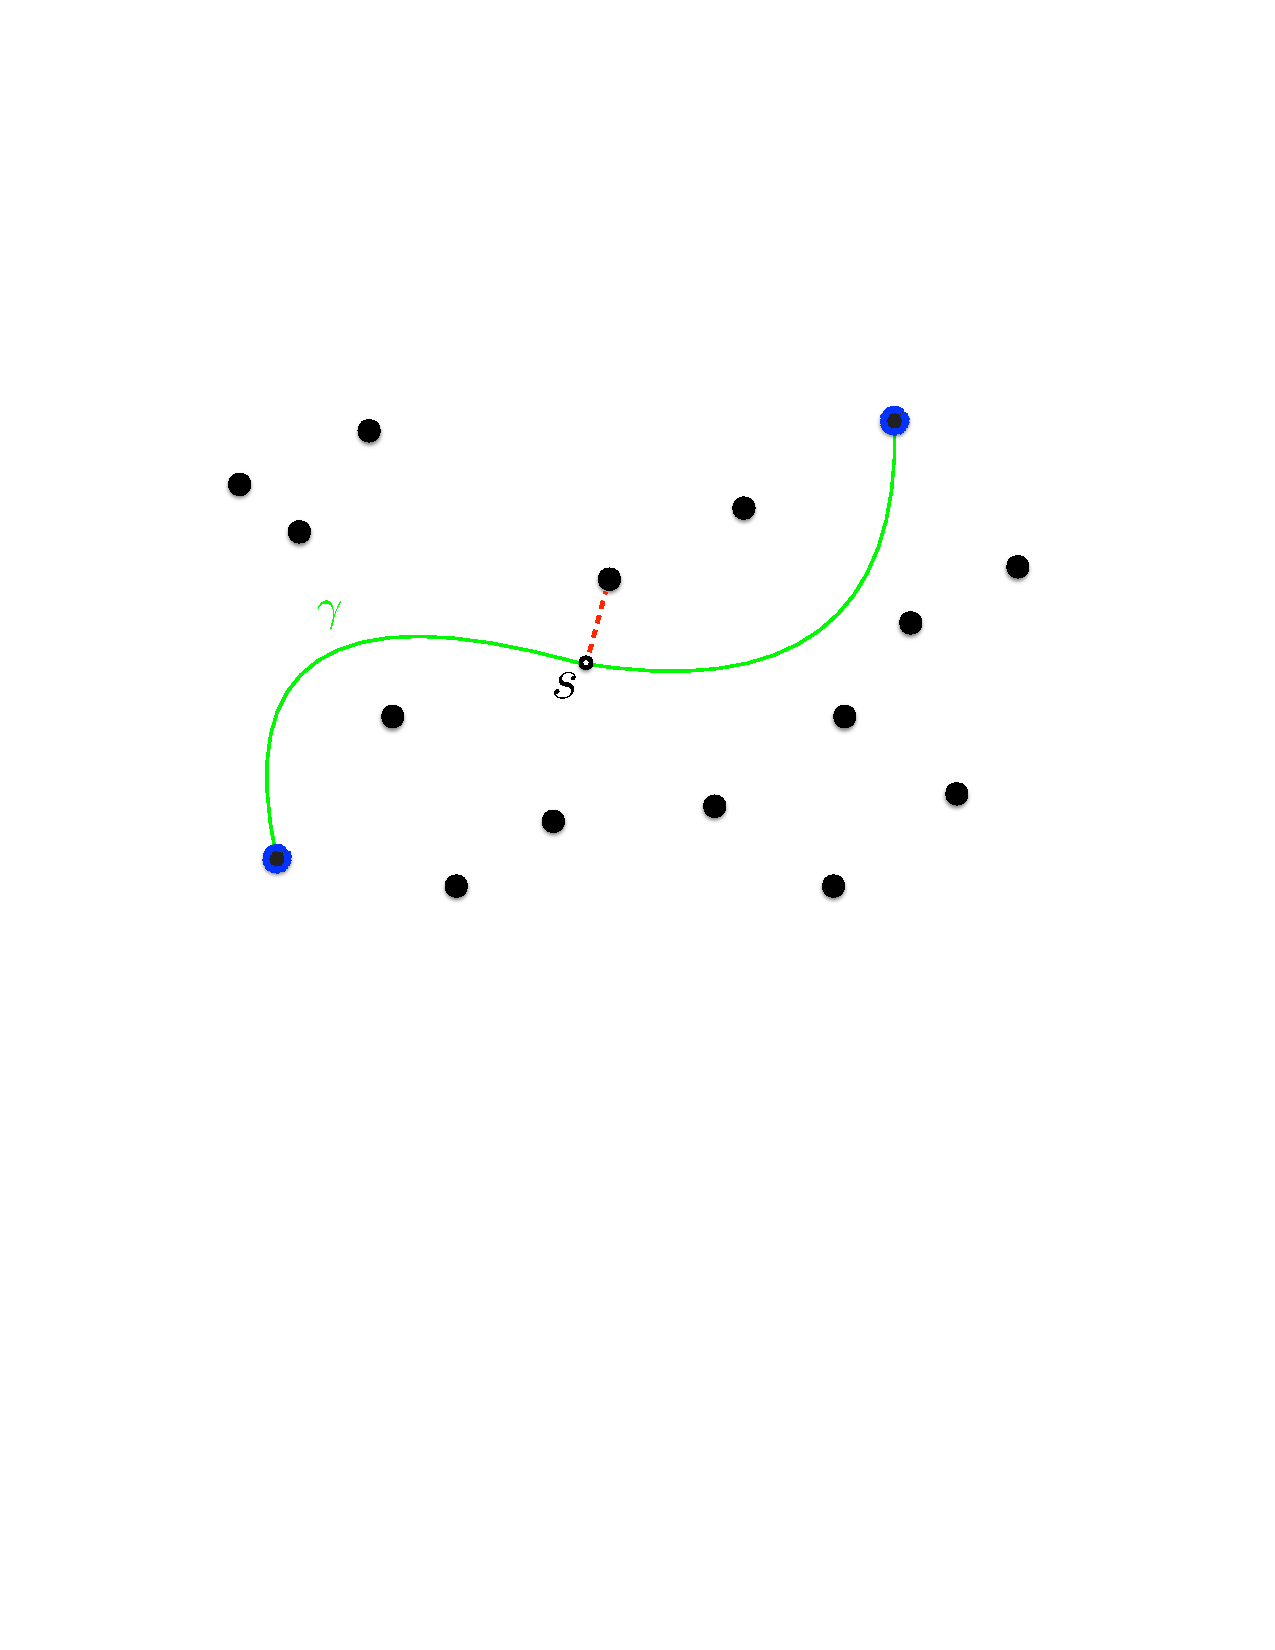
\includegraphics[width=0.3\textwidth]{screw/Figures/example.pdf}
    \caption{In this figure we have a collection of points.
      The length or cost of the green curve between the two blue points
      is the integral along the curve scaled by the distance to the nearest
point.}
  \label{fig:example}
\end{figure}

The nearest neighbor metric, and density-based distances in general, are
examples of manifold geodesics~\cite{sajama05estimatingDBDM,
tenenbaum00global}.  Manifold geodesics of data sets are
defined by embedding points into a manifold and computing the infimum
length path in the manifold.  Within computer science, dozens of
foundational papers in machine learning and surface reconstruction rely on
manifold-based metrics to perform clustering, classification, regression,
surface reconstruction, persistent homology, and
more~\cite{tenenbaum00global, cohen15approximating, vincent03,
bijral11semiSupLearningDBD,  sajama05estimatingDBDM,
edelsbrunner02topological, alamgir12shortest, vL09}.  Manifold geodesics
predate computer science, and are the cornerstone of many fields of physics
and mathematics.  Exactly computing geodesics is fundamental to countless
areas of physics including: the brachistochrone and minimal-drag-bullet
problem of Bernoulli and Newton~\cite{bernoulli}, exactly determining a particle's
trajectory in classical physics (Hamilton's Principle of Least
Action)~\cite{Courant53}, computing the path of light through a
non-homogeneous medium (Snell's law), finding the evolution of wave
functions in quantum mechanics over time (Feynman path integrals~\cite{Feynman48}), and
determining the path of light in the presence of gravitational fields
(General Relativity, Schwarzschild metric)~\cite{Schwarzschild, Sussmann97}. In
mathematics, manifold geodesics appear in many branches of higher
mathematics including differential equations, differential geometry, Lie
theory, calculus of variations, algebraic geometry, and topology.

One of the most significant problems on any manifold geodesic is how to
compute its length.  Exact computation of manifold metrics is considered a
fundamental problem in mathematics and physics, dating back for four
centuries: entire fields of mathematics, including the celebrated calculus
of variations, have arisen to tackle this~\cite{Courant53}. Historically,
mathematicians placed strong emphasis on exact computation as opposed to
constant factor approximations~\cite{Courant53}. An algorithmic problem on manifold
geodesics, with modern origins, is to $(1+\eps)$ approximate these metrics
efficiently on a computer.  The core difficulty in the first problem is
that geodesics are the minimum cost path out of an uncountable number of
paths that can travel 'anywhere' on the manifold structure.  This makes
exactly computing these metrics challenging, even in the case of the
nearest neighbor metric for just four fixed points in two dimensions (the
authors are unaware of any easy method for this simplified task).
% The core tool for exactly computing manifold metrics, calculus of
% variations, is intractable on the nearest neighbor metric due to the
% metric's heavy dependence on the Voronoi diagram of the point set, which
% can be quite complicated for even five points in two dimensions (for more
% on this approach and its limitations, see []).
Calculus of variations can show that the optimal nearest neighbor path is
piecewise hyperbolic, but this is generally insufficient to exactly compute
the nearest neighbor metric---there are point sets where there are
many differentiable, piecewise hyperbolic paths between two data points with
different costs.


In this chapter, we solve both problems: we exactly compute the Nearest
Neighbor metric in all cases, and we $(1+\eps)$ approximate it quickly.
Our approach is based on a novel embedding of the data into high dimensions where the geodesics are straight lines.
Then we use a Lipschitz extension theorem to relate the lengths of the shortest paths in the original space and the embedding.
We combine these tools to prove that the nearest neighbor metric is exactly equal to a shortest path distance on a geometric graph, the so-called edge-squared metric, in all cases.
This allows us to compute the nearest-neighbor metric exactly for any given point set in polynomial time, and it is the only known (non-trivial) density-based distance that can be computed by a discrete algorithm.

  \begin{definition}
For $x\in \R^d$, let $\|x\|$ denote the Euclidean norm.
  For a set of points $P\subset \R^d$:
  the \textbf{edge-squared metric} for $a,b\in P$ is
  \[
    \dist_2(a,b) = \inf_{(p_0,\ldots, p_k)}\sum_{i=1}^k \|p_i - p_{i-1}\|^2,
  \]
  where the infimum is over sequences of points $p_0,\ldots, p_k\in P$ with $p_0 = a$ and $p_k = b$.
  \end{definition}

\begin{theorem}\label{thm:NN} The nearest neighbor metric and edge squared
metric are equivalent for any set $P$ in arbitrary dimension that is the
finite collection of compact path-connected sets.
\end{theorem}

This in particular covers the case of $n$ points in $n-1$ dimension. The exact equality is realized when the nearest neighbor path is piecewise
linear, traveling straight from data point to data point.
The edge squared metric has been previously studied by multiple researchers
in machine learning and power-efficient wireless networks, but previously
has only been linked to the nearest neighbor metric by a fairly weak
3-approximation~\cite{cohen15approximating}.
There are several reasons why it is surprising that these metrics are equal:

\begin{enumerate}

\item The optimal nearest neighbor path for two points not in the dataset
is generally composed of hyperbolic arcs.
This holds true even when the dataset is a single point, and was established by~\cite{cohen15approximating} using tools in Riemannian surfaces and the complex plane.
Meanwhile, our Theorem implies an optimal nearest neighbor path for two
data points (in a dataset of any size) is piecewise linear!

\item There are simple and natural variants of the nearest neighbor metric, for which no analog of Theorem~\ref{thm:NN} is known nor suspected.
For example, if one considers powers (other than one) of the distance function as a cost, a corresponding graph-based metric is known to exist only for sets of size at most two.
% These variants are known as the $q$-nearest neighbor metric, for $1 < q < 2$, and we will formally define these
% metrics later in the introduction. When $q=2$, these
% metrics coincide with the nearest neighbor metric.
% This
% gives us a natural suite of metrics that smoothly converge
% to the nearest neighbor metric, for which no theorem like
% Theorem~\ref{thm:NN} is known.

\item For just three points in a right triangle configuration, there exist an uncountable suite of optimal-cost paths between the two endpoints of the hypotenuse.
Each path in this uncountable suite is piecewise hyperbolic, but, surprisingly, they all have the exact same cost as the edge-squared distance.
Thus, there shortest paths may not even be unique.
% Thus, lowering the nearest neighbor function anywhere inside the triangle and using this to build a new density-based distance will break Theorem~\ref{thm:NN}.
% This establishes that the equality in Theorem~\ref{thm:NN} is fairly tight.

 \item The finite union of compact path-connected geometric bodies in arbitrary
 dimension can have extremely complicated geometry, and the Voronoi diagram
on which the nearest neighbor metric depends is poorly understood for even
three of these bodies in two dimension.  There is no other restriction on
the compact geometric objects, and they need not be convex or even simply
connected, see figure~\ref{fig:example1}.
\begin{figure}[htbp]
  \centering
    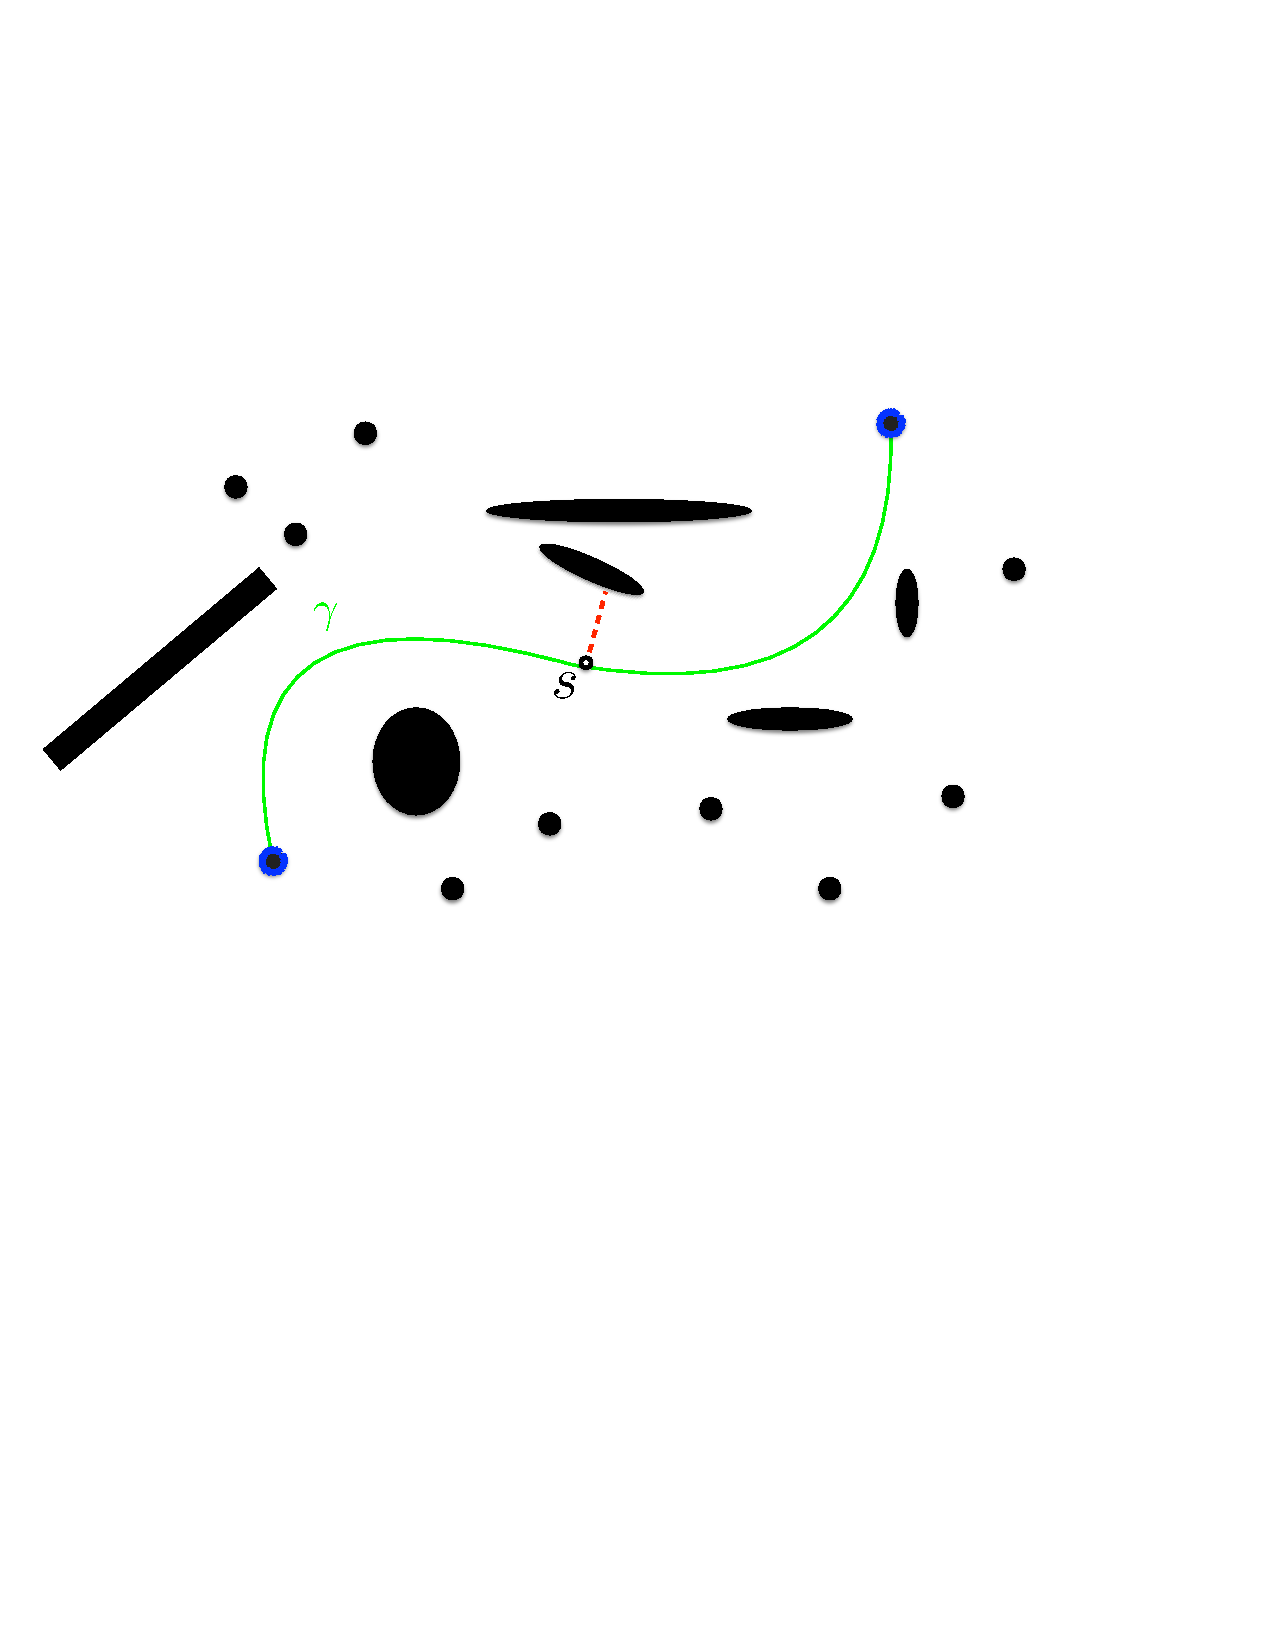
\includegraphics[width=0.3\textwidth]{screw/Figures/example1.pdf}
    \caption{In this figure we have a collection of compact bodies in black.
      The length or cost of the green curve between the two blue points
      is the integral along the curve scaled by the distance to the nearest body.
    A curve may traverse a body at  no cost. Theorem~\ref{thm:NN}
establishes that the shortest path curve between two points goes straight
from compact body to compact body.}
  \label{fig:example1}
\end{figure}
\end{enumerate}

We can now tackle a second problem of interest for manifold geodesics,
which is efficiently $(1+\eps)$ approximating them. In this chapter, we show
that the nearest neighbor metric admits $(1+\epsilon)$ spanners computable
in nearly-linear time, with linear size, for any point set in constant
dimension. Remarkably, these spanners are significantly sparser and faster
to compute than the theoretically optimal Euclidean spanners with the same
approximation constant, and nearly match the sparsity of the best known
Euclidean Steiner spanners. Moreover, if the point set comes from a
well-behaved probability distribution in constant dimension (a foundational
assumption in machine learning~\cite{hwang2016}), we show that the nearest neighbor
metric has perfect $1$-spanners of nearly linear size. The latter result is
impossible for many non-density sensitive metrics, such as the Euclidean
metric. Both results rely on Theorem~\ref{thm:NN}, and significantly
improve the nearest neighbor spanners of Cohen et al in~\cite{cohen15approximating}.

Theorem~\ref{thm:NN} and our spanner theorems solve two core problems of
interest for the nearest neighbor metric: exactly computing it for any
dimension, and approximating it quickly for both general point sets and
point sets arising from a well-behaved probability distribution in constant
dimension. This is the first work we know of that computes a manifold
metric exactly without calculus of variations, and we hope that our tools
can be useful for other metric computations and approximations.

% Besides for this contribution, we also generalize the nearest neighbor
% Metric to the $q$-nearest neighbor metric (abbreviated $q$-NN for short),
% and exactly compute this metric for all point sets with $\leq 4$ points for all $q>2$. We
% do this by equating it to the $q$-edge power metrics. Both the $q$-NN and
% $q$-edge power metrics will be defined later.
% \begin{theorem} \label{thm:qNN}
% For point sets that are the union of up to $4$ connected compact sets, the $q$-NN metric is exactly equal to
% the $q$-edge power metric when $q>2$. This equality is false for all $q <
% 2, q\not=1$.
% \end{theorem}
% Our equality is robust enough to handle the union of $4$ compact sets in
% any dimension. These unions
% ch can have very complicated geometry, and their Voronoi diagrams are in
% general difficult to understand. This is what makes theorems
% Theorem~\ref{thm:qNN} surprising. We further conjecture:
% \begin{conjecture}\label{conj:qNN}
% For any compact set, the $q$-NN metric is exactly equal to the $q$-edge
% poewr metric when $q>2$.
% \end{conjecture}
% If true, this would give us a quadratic algorithm to compute the $q$-NN
% metric for any $n$ point set.

% We further show that $q$-edge power metrics (and thus, it is hoped, the $q$-nearest neighbor metrics) are natural generalizations of maximum-edge-length distances on Euclidean MSTs, which in turn are fundamental for celebrated clustering methods like single-linkage clustering~\cite{}.
% This implies that the $q$-edge power metric, and the nearest neighbor metric, can be used to generalize popular methods in clustering.

  \subsection{Contributions and Past Work}
Our primary contribution is Theorem~\ref{thm:NN}, which lets us exactly
compute the nearest neighbor metric. This significantly strengthens a core
result of Cohen et al~\cite{cohen15approximating}. This theorem should be considered
quite surprising: it equates the nearest neighbor metric with the
edge-squared metric, even when the point set is a collections of compact,
path-connected objects in arbitrarily large dimension. There are no
restrictions on the convexity or simple-connectedness of such objects, so
in general the Voronoi diagram of these objects (on which the nearest
neighbor metric critically depends) can be extremely complicated.

 Besides for exactly computing the nearest neighbor metric, we present the
following theorems on approximate computation:

 %% \begin{theorem} \label{thm:NN} Given a point set $P \in \mathbb{R}^d$, the edge-squared metric on $P$
%%   and the nearest neighbor metric on $P$ are always equivalent.
%% \end{theorem}

\begin{theorem} \label{thm:general-spanner}
  For any set of points in $\mathbb{R}^d$ for constant $d$, there exists a $(1+\eps)$
  spanner of the nearest neighbor metric
  with size $O\left(n\eps^{-d/2} \right)$ computable in time
  $O\left(n \log n + n\eps^{-d/2}\log{\frac{1}{\eps}}\right)$. The
  $\log{\frac{1}{\eps}}$ term goes away given access to an algorithm
computing floor function
in $O(1)$ time.
\end{theorem}

\begin{theorem} \label{thm:distribution-spanner}
Suppose points $P$ in Euclidean space are drawn i.i.d from a Lipschitz probability density bounded
above and below by a constant, with support on a
smooth, connected, compact manifold with intrinsic dimension $d$ with boundary of bounded curvature. Then w.h.p. the $k$-NN graph of
  $P$ for $k = O(2^d \ln n)$ and edges weighted with Euclidean
  distance squared, is a $1$-spanner of the nearest neighbor
  metric on $P$.
\end{theorem}

These theorems rely on Theorem~\ref{thm:NN} and considerably strengthen the
spanner results on the nearest neighbor metric
from~\cite{cohen15approximating}. They critically rely on
Theorem~\ref{thm:NN}, which show it suffices to compute spanners of the
edge-squared metric.
Previously, sparse spanners of the edge-squared metric were shown to exist in two
dimensions via Yao graphs and Gabriel graphs~\cite{LiWan2001}, but these
did not generalize well to constant dimension: Yao
graphs are not very efficient to compute, and Gabriel graphs can have
quadratically many edges even in $3$ dimensions~\cite{chazelle94selecting}.
The spanners we produce are sparser than the
theoretical optimal for Euclidean spanners~\cite{Le19}.

Theorem~\ref{thm:distribution-spanner} proves that a $1$-spanner of
the nearest neighbor metric can be found assuming points are samples from a
probability density, by using a $k$-$NN$ graph for
appropriate $k$. Our result is tight when $d$ is constant. This
is not possible for Euclidean distance, as a $1$-spanner is almost
surely the complete graph. Although the restrictions on the probability
density may seem limiting,
they are in fact quite flexible and standard in
machine learning theory and practice~\cite{hwang2016, alamgir12shortest}. For example, although they do not cover the case
of a Gaussian (unbounded support), they do cover the case of a Gaussian
where the very thin tail is cut off, and this recovers most of the relevant
data in a Gaussian distribution. Past work on similar results
include~\cite{Balister05, Gonzales2003}.

Theorem~\ref{thm:NN} will additionally allow us
to compute the persistent homology of $\dist_N$, a task useful for
topological data analysis~\cite{edelsbrunner02topological}.
We also show how the nearest neighbor metric generalizes Euclidean
distance and maximum-edge Euclidean MST distance ~\cite{LiWan2001}

The core mathematical contribution of our work is the
statement and proof of Theorem~\ref{thm:NN}.  The techniques to prove
our other results are simpler and mostly leverage Theorem~\ref{thm:NN} and
past work. We have included them nonetheless to provide a more complete
picture of the nearest neighbor metric, and to provide possible directions for future
work.

%% Old outline: check this outline before submitting.
%% \begin{enumerate}
%% \item Definition of edge-squared.
%% \item Preliminaries
%% \item Outline/Overview/Previous Work
%% \item Interpretations based on known Machine Learning tools.
%% \begin{enumerate}
%% \item Gaussian Kernel similarity.
%% \item Generalization of Level-Set and Single-Linkage clustering. (\tim{This
%%     is not a very good point.})
%% \item Interpretation as $l_2$ on paths?
%% \end{enumerate}
%% \item Equality to a natural geodesic distance.
%% \begin{enumerate}
%% \item Define NN-metric.
%% \item Core Proof.
%% \item NN has a fast sparse spanner. Any spanner of the NN metric is a
%% spanner of edge-squared. (This result is theoretically
%%     superseded by our later result, but is of independent interest).
%% \item Persistent homology of the nearest neighbor metric can be
%% computed.
%% \end{enumerate}
%% \item Fast practical spanners for points in a distribution. ($k$-NN
%%     graph for $k = O( \log n)$.
%% \item Theoretically sparse, fast spanners for points in low dimension.  \tim{Low intrinsic dimension? Can cover trees do this for me?}
%% \item Remaining open questions.
%% \item Appendix:
%% \begin{enumerate}
%% \item Persistent homology can be put here, maybe.
%% \item Links to Heirarchies of Metrics: Edge-Squared is a natural
%% extension of negative type metrics, with potentially high doubling dimension.
%% \end{enumerate}
%%
%% \end{enumerate}

	% !TeX root = main.tex

\subsection{Definitions and Preliminaries} % (fold)
\label{sec:definitions}
In this section, we establish additional definitions for this chapter. These
are mostly of interest for our spanner and persistent homology results, and are not strictly
necessary for Theorem~\ref{thm:NN}.

%  \tim{Anything on wireless networks here? Or other prelims?}
\vspace{3 mm}

\noindent \textbf{Spanners:} For real value $t \geq 1$, a $t$-spanner of
a weighted graph $G$ is a subgraph $S$ such that $d_G(x,y) \leq d_S(x,y)
\leq t\cdot d_G(x,y)$ where $d_G$ and $d_S$ represent the shortest path
distance functions between vertex pairs in $G$ and $S$. Spanners
of Euclidean distances, and general graph distances, have been
studied extensively, and their importance as a data structure is
well established.
~\cite{Chew1986, Vaidya1991, Callahan1993,HarPeled13}.

\vspace{3 mm}
\noindent \textbf{$k$-nearest neighbor graphs:} The $k$-nearest neighbor graph
($k$-NN graph) for a set of objects $V$ is a graph with vertex set $V$
and an edge from $v\in V$ to its $k$ most similar objects in $V$, under
a given distance measure. In this chapter, the underlying distance
measure is Euclidean, and the edge weights are Euclidean distance
squared.
$k$-NN
graph constructions are a key data structure in machine
learning~\cite{Dong11, Chen11}, clustering~\cite{vL09}, and manifold learning~\cite{tenenbaum00global}.

\vspace{3 mm}
\noindent \textbf{Gabriel Graphs:} The Gabriel graph is a graph where
two vertices $p$ and $q$ are joined by an edge if and only if the disk
with diameter $pq$ has no other points of $S$ in the interior. The
Gabriel graph is a subgraph of the Delaunay
triangulation~\cite{SridharMaster}, and a
$1$-spanner of the edge-squared metric~\cite{SridharMaster}. Gabriel
graphs will be used in the proof of
Theorem~\ref{thm:distribution-spanner}.

\vspace{3 mm}
\noindent \textbf{Persistent Homology:}
  Persistent homology is a popular tool in computational geometry and topology to ascribe quantitative topological invariants to spaces that are stable with respect to perturbation of the input.
  In particular, it's possible to compare the so-called persistence diagram of a function defined on a sample to that of the complete space~\cite{chazal08towards}.
  These two aspects of persistence theory---the intrinsic nature of topological invariants and the ability to rigorously compare the discrete and the continuous---are both also present in our theory of nearest neighbor metrics.
  Indeed, our primary motivation for studying these metrics was to use them as inputs to persistence computations for problems such as persistence-based clustering~\cite{chazal13persistence} or metric graph reconstruction~\cite{aanjaneya12metric}.

% section definitions (end)

  \section{Outline}
%   Definitions of the nearest neighbor metric, and of the
%     edge-squared metric, are provided in
%    Section~\ref{sec:definitions}.
%
Section~\ref{sec:NN} contains the proof of Theorem~\ref{thm:NN},
equating the edge-squared metric and nearest neighbor metric in
all cases. It should be noted that our proof is robust enough to handle not
just finite point sets, but also countably infinite collections of disjoint
path-connected, compact sets. Remarkably, there is no restriction on the convexity or
simply-connectedness of these sets.

As an example of using the nearest neighbor metric to compute intrinsic structure, Section~\ref{sec:persistence} shows how Theorem~\ref{thm:NN} allows us to compute the persistent homology of the nearest neighbor metric.

Section~\ref{sec:edge-power} introduces the $p$-power metrics. We show
that Euclidean spanners and Euclidean MSTs are special cases of
$p$-power spanners. We show how
clustering algorithms including $k$-means, level-set methods,
and single linkage clustering, are special cases of
clustering with $p$-power metrics. $p$-power metrics are identical to the
Neighbor metric when $p=2$. This is further detailed in
Appendix~\ref{ap:clustering-link}.

Section~\ref{sec:general-spanner} outlines a proof of
Theorem~\ref{thm:general-spanner}, and compares our spanner to new lower
bounds on the sparsity of $(1+\eps)$-spanners of the Euclidean metric.  We
outline a proof of Theorem~\ref{thm:distribution-spanner} in
Section~\ref{sec:distribution-spanner} and discuss its implications.


Conclusions and open questions are in
Section~\ref{sec:conclusions}. Full proofs for
Theorems~\ref{thm:distribution-spanner},~\ref{thm:general-spanner}
are contained in the Appendix.

  \section{Exactly Computing the nearest neighbor metric}
\label{sec:NN}
In this section, we prove Theorem~\ref{thm:NN} on finite point sets, and
explain in Section~\ref{sec:bodies} that our proof strategy applies to
finite collections of path-connected compact bodies.

  First, lets observe what happens when $P$ has only two points $a$ and
$b$, $\dist_2(a,b) = \dist_N(a,b)$.  This reduces to a high school calculus
exercise as the minimum path $\gamma$ will be a straight line between the
points and the nearest neighbor metric is
\begin{align*}
  \dist_N(a,b) &= 4\int_0^1 \distto_P(\gamma(t))\|\gamma'(t)\|dt \\
  & = 8\int_0^{\frac{1}{2}} t \|a - b\|^2 dt = \|a - b\|^2 = \dist_2(a,b).
\end{align*}
  Now it is easy to observe that the
  nearest neighbor metric is never greater than the
  edge-squared distance, as proven in the following lemma.

  \begin{lemma}\label{lem:dist_N_le_dist}
    For all $s,p\in P$, we have $\dist_N(s,p)\le \dist_2(s,p)$.
  \end{lemma}
  \begin{proof}
    Fix any points $s,p\in P$.
    Let $q_0,\ldots, q_k \in P$ be such that $q_0 = s$, $q_k = p$ and
    \[
      \dist_2(s,p) = \sum_{i=1}^k \|q_i - q_{i-1}\|^2.
    \]
    Let $\psi_i(t) = tq_i + (1-t)q_{i-1}$ be the straight line segment from $q_{i-1}$ to $q_i$.
    Observe that $\len(\psi_i) = \|q_i - q_{i-1}\|^2 / 4$, by the same argument as in the two point case.
    Then, let $\psi$ be the concatenation of the $\psi_i$ and it follows that
    \[
      \dist_2(s,p) = 4 \len(\psi) \ge 4 \inf_{\gamma\in \ourpath(s,p)} \len(\gamma) = \dist_N(s,p).
    \]
  \end{proof}

  By Lemma~\ref{lem:dist_N_le_dist}, it suffices to show that $\dist_N(a, b) \geq \dist_2(a,b)$ for all $a, b \in P$.
% This allows us to compute of the nearest neighbor metric exactly by instead computing the edge-squared metric.
%\subsection{Equivalence} % (fold)
\label{sec:the_proof}

  Let $P\subset \R^d$ be a set of $n$ points.
  Pick any \emph{source} point $s\in P$.
  Order the points of $P$ as $p_1,\ldots ,p_n$ so that
  \[
    \dist_2(s,p_1) \le \cdots \le \dist_2(s, p_n).
  \]
  This will imply that $p_1 = s$.
  It will suffice to show that for all $p_i\in P$, we have $\dist_2(s,p_i) = \dist_N(s,p_i)$.
  There are three main steps:
  \begin{enumerate}
    \item We first show that when $P$ is a subset of the vertices of an axis-aligned box, $\dist = \dist_N$.  In this case, shortest paths for $\dist$ are single edges and shortest paths for $\dist_N$ are straight lines.
    \item We then show how to lift the points from $\R^d$ to $\R^n$ by a Lipschitz map $m$ that places all the points on the vertices of a box and preserves $\dist_2(s,p)$ for all $p\in P$.
    \item Finally, we show how the Lipschitz extension of $m$ is also Lipschitz as a function between nearest neighbor metrics.  We combine these pieces to show that $\dist \le \dist_N$.  As $\dist \ge \dist_N$ (Lemma~\ref{lem:dist_N_le_dist}), this will conclude the proof that $\dist = \dist_N$.
  \end{enumerate}
The key to the second step, to be elaborated in Section~\ref{sec:lifting},
is that if you take points on a line and raise the pairwise distances to
the $1/2$ power, you get points on a box. This is a special case of the
general theory on screw functions developed by Von Neumann and Schoenberg,
which asserts a far more general criterion on when functions applied to
pairwise distances between points on a line can be embedded into Euclidean
space~\cite{VonNeumann41}.
  \input{screw/boxes-soda}
  \input{screw/lifting-soda}
  \input{screw/lip_extension-soda}
\subsection{From Finite Sets to Finite Collections of Compact Path-Connected Bodies}
\label{sec:bodies}
All of our proof steps hold for finite collections of compact,
path-connected bodies in arbitrarily large dimension. Our Lipschitz map $m$ can
still be extended to a Lipschitz map $f$ in this setting, largely due to the
generality of the Kirszbraun theorem. In this case, the pre-image of the
contractive map is the set of all points belonging to some body. Meanwhile, the image is a finite set of points, the corners of a multi-dimensional box.
Thus our construction of $m$ contracts each convex
body into a single point, and the image of our
compact bodies under $f$ is still a finite point set on the corners of a
box. Therefore, the remainder of our theorem proof goes through unchanged.

This result is rather remarkable: path-connected compact sets in high
dimensional space can have extremely convoluted geometry, and the Voronoi diagrams
on these collections (on which the nearest neighbor metric depends) can be
massively complex.  The key is that our Lipschitz map is robust enough to
handle objects of considerable geometric complexity.
  
  
% section the_proof (end)


  \section{Persistent Homology of the Nearest-neighbor Geodesic Distance}
  \label{sec:persistence}

% \tim{This section should be prefaced somewhere -- here or in a previous
% section -- with a statement as to why the nearest neighbor metric may
% still be of independent interest. My main claim is that it's useful
% since it's defined on all points rather than just two.}
%
% \tim{My main issue with this section is that I don't have a clean
% theorem saying how to compute persistent homology, both in ambient and
% intrinsic setting. Having one or two top-level theorems that say this
% would be great, rather than having it be written in the exposition. As
% it stands, I have no clue how Lemma 4.5 is used, or Lemma 4.6, to
% compute the homologies.}
  In this section, we show how to compute the so-called persistent homology~\cite{edelsbrunner02topological} of the nearest neighbor metric in two different ways, one ambient and the other intrinsic.
  The latter relies on Theorem~\ref{thm:NN} and would be quite surprising without it.

  The input for persistence computation is a \emph{filtration}---a nested sequence of spaces, usually parameterized by a real number $\alpha\ge 0$.
  The output is a set of points in the plane called a \emph{persistence diagram} that encodes the birth and death of topological features like connected components, holes, and voids.

  \paragraph*{The Ambient Persistent Homology}

    Perhaps the most popular filtration to consider on a Euclidean space is the sublevel set filtration of the distance to a sample $P$.
    This filtration is $(F_\alpha)_{\alpha\ge 0}$, where
    \[
      F_\alpha := \{x\in \R^d \mid \distto_P(x) \le \alpha\},
    \]
    for all $\alpha \ge 0$.
    If one wanted to consider instead the nearest neighbor metric $\dist_N$, one gets instead a filtration $(G_\alpha)_{\alpha\ge 0}$, where
    \[
      G_\alpha := \{x\in \R^d \mid \min_{p \in P} \dist_N(x,p) \le \alpha\},
    \]
    for all $\alpha \ge 0$.

    Both the filtrations $(F_\alpha)$ and $(G_\alpha)$ are unions of metric balls.
    In the former, they are Euclidean.
    In the latter, they are the metric balls of $\dist_N$.
    These balls can look very different, for example, for $\dist_N$, the metric balls are likely not even convex.
    However, these filtrations are very closely related.
    \begin{lemma}
      For all $\alpha \ge 0$, $F_\alpha = G_{2\alpha^2}$.
    \end{lemma}
    \begin{proof}
      The key to this exercise is to observe that the nearest point $p \in P$ to a point $x$ is also the point that minimizes $\dist_N(x,p)$.
      To prove this, we will show that for any $p\in P$ and any path $\gamma\in \ourpath(x,p)$, we have $\len(\gamma)\ge \frac{1}{2}\distto_P(x)^2$.
      Consider any such $x$, $p$, and $\gamma$.
      The euclidean length of $\gamma$ must be at least $\distto_P(x)$, so we will assume that $\|\gamma'\| = \distto_P(x)$ and will prove the lower bound on the subpath starting at $x$ of length exactly $\distto_P(x)$.
      This will imply a lower bound on the whole path.
      Because $\distto_P$ is $1$-Lipschitz, we have $\distto_P(\gamma(t))\ge (1-t)\distto_P(x)$ for all $t\in [0,1]$.  It follows that
      \begin{align*}
        \len(\gamma) &= \int_0^1 \distto_P(\gamma(t))\|\gamma'(t)\|dt \\
         &  \ge \distto_P(x)^2 \int_0^1 (1-t)dt
          =  \frac{1}{2}\distto_P(x)^2
      \end{align*}
      The bound above applies to any path from $x$ to a point $p\in P$, and so,
      \[
        \dist_N(x,p) = 4 \inf_{\gamma\in \ourpath(x,p)} \len(\gamma) \ge 2\distto_P(x).
      \]
      If $p$ is the nearest neighbor of $x$ in $P$, then $\dist_N(x,p) = 2\distto_P(x)$, by taking the path to be a straight line.
      It follows that $\min_{p\in P}\dist_N(x,p) = 2\distto_P(x)$.
    \end{proof}

    The preceding lemma shows that the two filtrations are equal up to a monotone change in parameters.
    By standard results in persistent homology, this means that their persistence diagrams are also equal up to the same change in parameters.
    This means that one could use standard techniques such as $\alpha$-complexes~\cite{edelsbrunner02topological} to compute the persistence diagram of the Euclidean distance and convert it to the nearest neighbor metric afterwards.
    Moreover, one observes that the same equivalence will hold for variants of the nearest neighbor metric that take other powers of the distance.

    % (some are considered in Section~\ref{sec:higher_powers}).


  \paragraph*{Intrinsic Persistent Homology}
    Recently, several researchers have considered intrinsic nerve complexes on metric data, especially data coming from metric graphs~\cite{adamszek16nerve,gasparovic17complete}.
    These complexes are defined in terms of the intersections of metric balls in the input.
    The vertex set is the input point set.
    The edges at scale $\alpha$ are pairs of points whose $\alpha$-radius balls intersect.
    In the intrinsic \v Cech complex, triangles are defined for three way intersections, tetrahedra for four-way intersections, etc.

    In Euclidean settings, little attention was given to the difference between the intrinsic and the ambient persistence, because a classic result, the Nerve Theorem~\cite{borsuk48imbedding}, and its persistent version~\cite{chazal08towards} guaranteed there is no difference.
    The Nerve theorem, however, requires the common intersections to be contractible, a property easily satisfied by convex sets such as Euclidean balls.
    However, in many other topological metric spaces, the metric
    balls might not be so well-behaved.
    In particular, the nearest neighbor metric has metric balls which may take on very strange shapes, depending on the density of the sample.
    This is similarly true for graph metrics.
    So, in these cases, there is a difference between the information in the ambient and the intrinsic persistent homology.

    \begin{theorem}
      Let $P\subset \R^d$ be finite and let $\dist_N$ be the nearest neighbor metric with respect to $P$.
      The edges of the intrinsic \v Cech filtration with respect to $\dist_N$ can be computed exactly in polynomial time.
    \end{theorem}
    \begin{proof}
      The statement is equivalent to the claim that $\dist_N$ can be computed exactly between pairs of points of $P$, a corollary of Theorem~\ref{thm:equality}.
      Two radius $\alpha$ balls will intersect if and only of the distance between their centers is at most $2\alpha$.
      The bound on the distance necessarily implies a path and the common intersection will be the midpoint of the path.
    \end{proof}

  \section{Relating the nearest neighbor metric to Euclidean MSTs,
Euclidean Spanners, and More}\label{sec:edge-power}
The nearest neighbor metric, as seen in Theorem~\ref{thm:NN}, is equal to
the edge-squared metric. This allows us to connect this manifold distance
to a graph distance, which we will in turn show is a generalization of
maximum-edge distance on minimum spanning trees. The results in this
section are quite simple to prove, but we nonetheless believe they are important
properties of the Nearest Neighbor metric and its variants.

The edge-squared metric on a Euclidean point set, as we recall, is defined by taking the
Euclidean distances squared and finding the shortest paths. 
We could have taken any such power $p$ of the Euclidean distances. We
will soon see that taking $p = 1$ gives us the Euclidean distance, and
finding spanners of the graph as $\lim p\rightarrow \infty$ is the
Euclidean MST problem.  
Let the $p$-power metric be defined on a Euclidean point set by taking
Euclidean distances to the power of $p$, and performing all-pairs
shortest path on the resulting distance graph.
\begin{theorem} \label{thm:1-spanner}
For all $q > p$, any $1$-spanner of the $p$-power metric is a
$1$-spanner of the $q$-power metric on the same point set
\end{theorem}
\begin{proof}
A $1$-spanner of the $q$-power metric can be made by taking
  edges $uv$ where
  \begin{align}\label{eq:span}
    \min_{p_0=u, \ldots p_k=v, k \not= 1} \sum_k ||p_i - p_{i-1}||^q > || u -
v||^q.
  \end{align}
If
  $\sum_{i=1}^k ||p_i - p_{i-1}||^q > || u - v||^q$ for any points
  $p_1, \ldots p_k$, then
  $\sum_{i=1}^k ||p_i - p_{i-1}||^p > || u - v||^p$ for any $q > p$.
  Thus, for all such edges $uv$ satisfying
  Equation~\ref{eq:span}:
  \[ \min_{p_0=u, \ldots p_k=v, k \not= 1} \sum_k ||p_i - p_{i-1}||^p > || u -
  v||^p. \] Such edges $uv$ must be included in any $1$-spanner
  of the $p$-power
  metric.
\end{proof}

 \begin{corollary}
   Let $P$ be a set of points in Euclidean space drawn i.i.d. from a Lipschitz
   probability density bounded above and below, with support on a
   smooth, compact manifold with intrinsic dimension $d$, bounded
   curvature, and
   smooth boundary of bounded curvature. Then the $k$-NN graph on $P$
   when $k = O(2^d \log n)$ is a $1$-spanner of the $p$-power
   metric for every $p \geq 2$, w.h.p.
 \end{corollary}
This follows from combining Theorem~\ref{thm:distribution-spanner} and
Theorem~\ref{thm:1-spanner}.
\subsection{Relation to the Euclidean MST problem}
  \begin{definition}
  Let the \textbf{normalized $p$-power metric} between two points in
  $\mathbb{R}^d$ be the $p$-power metric between the two points,
  raised to the $\frac{1}{p}$ power. Define the normalized $\infty$-power
  metric as the limit of the normalized $p$-power metric as $p \rightarrow \infty$.
  \end{definition}
  \begin{lemma} The Euclidean MST is a
  $1$-spanner for the normalized $\infty$-power metric.
  \end{lemma}
  This lemma follows from basic properties of the MST.
  The normalized $p$-power metrics give us a suite of
  metrics such that $p=1$ is the Euclidean
  distance and $p=\infty$ gives us the distance of the longest edge on the
  unique MST-path.  Setting $p=2$ gives the edge-squared metric, which
  sits between the Euclidean and max-edge-on-MST-path distance. 
  Theorem~\ref{thm:1-spanner} establishes
  that minimal $1$-spanners of the (normalized) $p$-power
  metric are contained in each other, as $p$ varies from
  $1$ to $\infty$. The minimal spanner for a general point set when $p=1$ is the complete graph, and
 the Euclidean MST is the minimal spanner for $p=\infty$. Thus:
  \begin{theorem} 
    For points in $\mathbb{R}^d$, every $1$-spanner of the $p$-power
    metric on that set of points contains every Euclidean MST.
  \end{theorem}
  \begin{corollary}
    Every $1$-spanner for the Nearest Neighbor metric
    contains every Euclidean
    MST. 
  \end{corollary}
  \subsection{Generalizing Single Linkage Clustering, Level Sets, and k-Centers
  clustering}
  If our point set is drawn from a well-behaved probability
  density, then the normalized edge-power metrics
  converge to a nice geodesic distance detailed
  in~\cite{hwang2016}. When $p=1$, clustering with this metric is
  the same as Euclidean metric clustering ($k$-means,
  $k$-medians, $k$-centers), and when $p=\infty$, clustering with
  this metric is the same as the single-linkage clustering and the widely
used level-set method~\cite{Wishart69, Gower1969, Ester1996,OPTICS96}.
Thus, clustering with normalized edge-power metrics generalizes these two
very popular methods, and interpolates between their advantages.
Definitions of the level-set method and a full discussion are contained in
Appendix~\ref{ap:clustering-link}

% \tim{Maybe you want to mention the self-sparsifying graph when you raise
% $p$ from $1$ to $\infty$}

% Kicked edge-power to appendix
  \section{Spanners for the nearest neighbor metric}
In this section, we prove our theorems on spanners of the nearest neighbor
metric. The proofs of these theorems mostly leverage Theorem~\ref{thm:NN}
and past work on geometric spanners. We have nonetheless included them
for completeness, and to illustrate that spanners of
manifold distances like the nearest neighbor metric can have interesting
properties not found in Euclidean spanners (assuming no Steiner points).
\subsection{Exact-spanners of nearest neighbor metric in
the Probability Density Setting
}\label{sec:distribution-spanner}
% \tim{Do a warm up on Gabriel graphs with convex support.}

Theorem~\ref{thm:distribution-spanner} states that for $k= O(2^d \log n)$, the $k$-NN graph of $n$ points drawn i.i.d from
a nicely behaved probability distribution is a $1$-spanner of the
nearest neighbor metric. This section is dedicated to outlining a proof of
this Theorem, the full result which will be in
Appendix~\ref{ap:distribution-spanner}.
This result is clearly impossible for Euclidean distances,
whose $1$-spanner is the complete graph almost surely.  
Our theorem implies any off-the-shelf
$k$-nearest neighbor graph generator can compute
edge-squared metric.  We strongly rely on Theorem~\ref{thm:NN} for this
result, and the fact that Gabriel graphs are $1$-spanners of the
edge-squared metric.

First, let us assume that the support of our
probability density $D$ has the same dimension as our ambient space.
This simplifies our calculations without changing the problem
much. Then, we note that as our number of sample points get
large, the density inside a $k$-NN ball around any point $x$ (the ball with radius
$k^{th}$-NN
distance, center at $x$) looks like the uniform distribution
on that ball, possibly intersected with a halfspace. The bounding
plane of our halfspace
represents the boundary of our density $D$.

For simplicity in the outline, let's suppose that $D$ is convex.
If we condition on
the radius of the $k$-NN ball, then the $k-1^{st}$ nearest
neighbors of $x$ are distributed roughly according to the above
distribution, described by the ball intersected with a halfspace.
For any other point $p$ in $D$, we project $p$ onto the $k$-NN
ball to point $p'$, and show that the ball $p'x$ contains a $k^{th}$ nearest
neighbor w.h.p, when $k=O(2^d \log n)$. This
implies ball with diameter $px$ contains a $k^{th}$ nearest
neighbor of $x$, and thus $px$ is not necessary in any
$1$-spanner of the edge-squared metric. Then we take union bound
over all $x$.
A rigorous proof of
Theorem~\ref{thm:distribution-spanner} requires careful analysis, 
and is contained in
Section~\ref{ap:distribution-spanner}.  
Our proof can be tweaked to show:
\begin{theorem}
  Given a Lipschitz distribution bounded above and below with support on convex set $C \subset
  \mathbb{R}^d$, the $k$-NN graph is Gabriel w.h.p. for $k =
  O(2^d \log n)$.
\end{theorem}

\subsection{Fast, Sparse Spanner for the Edge-Squared
Metric}
\label{sec:general-spanner}

Now we outline a proof for Theorem~\ref{thm:general-spanner}, which shows
that one can construct a $(1+\eps)$ nearest neighbor metric spanner of size
$O(n \eps^{-d/2})$ in
time $O\left(n \log n + n \eps^{-d/2} \log \left(\frac{1}{\eps}\right)\right)$, 
for points in constant dimensional space. The full proof is in
Appendix~\ref{ap:general-spanner}. We critically rely on
Theorem~\ref{thm:NN} for this work, which shows
a spanner for the edge-squared metric is equivalent to a spanner for the
nearest neighbor metric.

Note that this spanner is sparser and faster in terms of epsilon dependency
than the theoretical optimal spanner for Euclidean distances~\cite{Le19}.
We rely extensively on well-separated pair decompositions
(WSPDs),
and this outline assumes familiarity with that notation.
For a comprehensive set of definitions and notations on well separated
pairs, refer to any of \cite{Callahan1995, Arya2016, Callahan1993,
arya95euclid}.  
Our proof consists of three parts.
\begin{enumerate}
\item Showing that connecting a $(1+O(\delta^2))$-approximate shortest edge
in a $1/\delta$ well separated pair for all the pairs in the decomposition
gives a $1+O(\delta^2)$ edge-squared spanner.
The processing for this step takes $O(n \log n + \delta^{-d}n)$ time.
\item Previous work contains an algorithm computing
  $1+O(\delta^2)$-approximate shortest edge in a $1/\delta$ well
    separated pair for all the pairs in a WSPD, and takes
    $O(1)$ time per pair. The pre-processing for this step will be
    bounded by $O(\delta^{-d}n\log\left(\frac{1}{\delta}\right))$ time. The $\log\left(\frac{1}{\delta}\right)$ factor goes away given a fast floor function. 
    This procedure was first introduced in~\cite{Callahan1995}.

\item Putting these two together, and setting $\epsilon = \delta^2$
gives us a $1+\epsilon$ spanner with
$O(\epsilon^{-d/2}n)$ edges in
    $O(n \log n + \epsilon^{-d/2}n)$ time.
\end{enumerate}
Full details of this proof are contained in Appendix~\ref{ap:general-spanner}


  \section{Conclusions and Open Questions}\label{sec:conclusions}


We examined the nearest neighbor metric and showed how to compute it
exactly, as well as find sparse data structures efficiently for approximate
computation in practice.  Many problems remain open.

First: are there generalizations of these metrics, for which our proof techniques
will still hold? The nearest neighbor metric has many natural
generalizations, including the $k^{th}$ nearest neighbor or powers of the
nearest neighbor function.

Can we efficiently compute $o(\log n)$-spanners of the nearest neighbor
metric in high dimension, such the the spanners have a nearly linear number of edges?
The existence of such spanners has been studied for Euclidean metrics in~\cite{HarPeled13}, where the stretch
obtained is $\sqrt{\log n}$.

Does computing $k$-NN graphs with approximate nearest neighbor methods give $1$-spanners of the
edge-squared metric with high probability?
Approximate nearest neighbors have been studied extensively
~\cite{kNNsurvey, Chen11, Dong11}, including locality-sensitive
hashing for high dimensional point sets~\cite{LSH} and
more~\cite{Laarhoven2018}.
Recent work by Andoni et al.~\cite{Andoni2018} showed how to compute
approximate nearest neighbors for any non-Euclidean norm.  Perhaps there
is a rigorous theory about data-sensitive metrics generated from any such
norm? Similar to
how the edge-squared metric is generated from the Euclidean distance.

It remains an open question how well clustering or
classification with
nearest neighbor metrics performs on real-world
data.
Experiments have been done by Bijral, Ratliff, and
Srebro in~\cite{bijral11semiSupLearningDBD}.
Theorem~\ref{thm:distribution-spanner} implies that future experiments
can be done using any
k-nearest-neighbor graph.  
  We believe that the interest in alternative metrics on Euclidean data will continue to be a rich source of interesting problems.

%%   We showed that the class of metrics that can be represented in this way is quite large, including all negative-type metrics and more.
%%   There is no constant upper bound on the doubling dimension of such metrics even for point sets in the plane.
%%   Theorem~\ref{thm:equality} extends these results immediately to density-based distances.
%%   Although there is such rich structure in these metrics, they still maintain some of the advantages of low-dimensional euclidean metrics, and this is exploited to generate sparse spanners.
%%   We also use the Euclidean structure to compute the persistent homology of the nearest neighbor distance in both the ambient sense and the intrinsic sense.
%%
%%   Many interesting problems remain open.
%%   One of the most compelling is the generalization of Theorem~\ref{thm:equality} to higher power metrics.
%%   It seems possible that integrating higher powers of the distance function could correspond exactly to higher power metrics.
%%   However, the proof techniques of this paper do not easily extend to that case.
%%   It does seem that as the power goes to infinity, shortest paths converge to the minimum spanning tree.
%%   For other powers in between $2$ and $\infty$, this question remains open.


% \begin{appendices}
  \appendix
    \section{Nearest Neighbor Metric and Edge-Power Metrics relate to Single Linkage Clustering, Level Sets, and k-Centers
  clustering}\label{ap:clustering-link}

  Many popular clustering algorithms, including $k$-centers, $k$-means,
  and $k$-medians clustering, use Euclidean distance as a measure of
  distance between points in $\mathbb{R}^d$. These methods are useful
  when clusters are spherical and well-separated. However, it is believed by
  practitioners that
  data-sensitive distances more accurately capture intrinsic
  distances between data \cite{alamgir12shortest}.

  The celebrated single-linkage clustering algorithm~\cite{Gower1969, Yaro2017},
  which is clustering based on an MST, is a widely used tool in
  machine learning, and gets around many of the problems of the
 Euclidean distance clustering. In single-linkage clustering,
   two points are considered similar if the maximum length
   edge on the path between them in the MST is small. This turns out to be equivalent to 
  computing the normalized $\infty$-power metric between the two
  points. Therefore, single linkage clustering can be seen
  as clustering using the normalized $\infty$-power metric.
  Generally, normalized $p$-power metrics can be seen as an
  intermediary between Euclidean distances ($1$-power metrics) and
  Euclidean MST-based clustering.

  Clustering with $p$-power metric relates to another popular
 clustering method in machine learning, known as level-set clustering.
  Loosely speaking, level set clustering involves finding an estimate
  for the probability density that points are drawn from, finding a
  cut threshold $t$, and then taking as clusters all regions with
  probability density $ > t$. Level set clustering
  has appeared in many incarnations~\cite{Wishart69, Stuetzle2003, Stuetzle2007}, including the celebrated and
  widely used DBScan method~\cite{Ester1996} and its
  considerable number of variations~\cite{OPTICS96}.
It is known
  that level-set clustering is related to single-linkage clustering, as
  the latter is an approximation of the former~\cite{Wishart69,
  Stuetzle2007}.  
  Level-set methods
  have the advantage that they can find arbitrarily shaped
  clusters~\cite{Ester1996}, but can cause two points that are very
  close in Euclidean distance to be considered far apart. 

  Clustering with the $p$-power metric incorporates the
  advantages of both Euclidean distance clustering and level set
  clustering, as it is both data-sensitive and takes into account
  overall
  Euclidean distance between two points.
  Here, $p$ can be toggled to change the sensitivity of the metric
  to the underlying density.
  As the number of samples
  drawn from our probability density grows large, it has been proven that the behavior of
  normalized $p$-power metrics converges to a natural geodesic distance on the
  underlying probability density~\cite{hwang2016}. Clustering with
  this geodesic distance for $p=1$ is exactly Euclidean clustering, and for
  $p=\infty$ is exactly the level set method. 
   Thus, clustering with $p$-power metric converges to
  a clustering method that smoothly interpolates between
  Euclidean-distance clustering and level set clustering. 
% \tim{Maybe you want to mention the self-sparsifying graph when you raise
% $p$ from $1$ to $\infty$}

\section{Proving Faster and Sparser-than-Euclidean Approximate
  Spanners}\label{ap:general-spanner}
In this appendix, we finish the proof of
Theorem~\ref{thm:general-spanner} based on the outline given in
Section~\ref{sec:general-spanner}.

\subsection{$1+O(\delta^2)$ spanners can be generated from a
$1/\delta$ WSPD}

\begin{definition}\label{def:critical} Let $e$ be a \textbf{critical} edge in a
  shortest path metric on any graph if the
  (possibly-not-unique) shortest path between the endpoints of $e$ is the edge $e$.
\end{definition}
\begin{lemma} The set of critical edges on any graph forms a $1$-spanner of the
shortest path metric. \end{lemma}
The above lemma is known in the literature.

% \tim{Make an algorithm box for this process.}
To check that any graph $H$ is a $(1+O(\delta^2)$ spanner of any graph $G$, it suffices
to prove that all critical edges in the edge-squared metric have a stretch
no larger than $1+O( \delta^2)$.
Let $G$ be the edge-squared graph arising from points $P \subset \mathbb{R}^d$. Build a well-separated pair decomposition on P, with pairs given as $\{A_1, B_1\}, \{A_2, B_2\}, \ldots \{A_m, B_m\}$.
Create a spanner $H$ as follows: for each pair $\{A_i, B_i\}$, connect
an edge $\{a, b\}, a\in A_i, b\in B_i$ such that the Euclidean distance
between $a$ and $b$ is a $(1+c\delta^2)$ approximation of the shortest distance
between point sets $A_i$ and $B_i$, for some constant $c$ independent of
$i$. This can be accomplished in $O(1)$ time assuming a preprocessing
step of $O(\delta^{-d} \log\left(\frac{1}{\delta}\right)$ time, as noted
in Callahan's paper on constructing a Euclidean MST~\cite{Callahan1995}. Do this for all $ 1 \leq i \leq m$.

For each critical edge $(s,t)$, consider the well-separated pair $\{A, B\}$ that $(s,t)$ is part of. Let $ s\in A$ and $t \in B$. Let $(a,b)$ be a $(1+c\delta^2)$-approximate shortest edge between $A$ and $B$ ($a \in A, b\in B$).
Scale $||a-b||_2$ to be 1. $A$ and $B$ have Euclidean radius at most
$\delta$, by the definition of a well separated pair. By induction on
Euclidean distance, $H$ is an edge-squared $2$-spanner of the
edge-squared metric for all points in $A$ and $B$ and all points in $B$
(assuming sufficiently small $\delta$).

\begin{lemma}
\begin{align*}
  dist_H(s,t)
    &\leq dist_H(s,a)+dist_H(a,b)+dist_H(b,t)\\
    & \leq 1+O(\delta^2)
\end{align*}
\end{lemma}
\begin{proof}
We know $dist_H(a,b)$ = 1 by our scaling, and $$dist_H(s,a) \leq 2 \cdot (dist_G(s,a)) \leq 2 \cdot ||s-a||^2 \leq 8\delta^2$$
The first inequality follows by the inductive hypothesis that $H$ is a 2-spanner of $G$ in $A$. The third inequality follows since both $s$ and $a$ are contained in a ball of radius $\delta$.

The same bound applies for $dist_H(b,t)$.
\end{proof}

\begin{lemma} \label{lm}
$$(1+c\delta^2)(dist_G(s,t)) \geq dist_G(a,b) = 1$$
$$ \Rightarrow dist_G(s,t)  \geq \frac{1}{1+c\delta^2}$$
\end{lemma}

Lemma \ref{lm} follows from the fact that $(a,b)$ is a $(1+c\delta^2)$ approximate shortest distance between $A$ and $B$.

Therefore

\begin{align*}
  stretch_H(s,t)
    &\leq \frac{dist_H(s,t)}{dist_G(s,t)} \\
    &\leq (1+16\delta^2)(1+c\delta^2) \\
    &= 1+O(\delta^2)
\end{align*}


Thus we have proven that $H$ is a $1+16\delta^2$ spanner. Now set
$\epsilon = \delta^2$, which completes
proof of Theorem~\ref{thm:general-spanner}.

\section{Spanners in the Probability Density Setting: Full
  Proof}\label{ap:distribution-spanner}

We prove Theorem~\ref{thm:distribution-spanner} in full.
Through this section, we assume that $D$ is a probability density
function with support on smooth connected compact manifold with intrinsic dimension
$d$ embedded in ambient space $\mathbb{R}^s$,
with smooth boundary of bounded curvature. This
probability density function is further assumed to be bounded
above and below, and to be Lipschitz. For simplicity, we assume that
$s=d$, and we can prove all our results when $s > d$ by taking
coordinate charts from the manifold into Euclidean space.  We
will show at the end of the section that if the distribution is
supported on a convex set of full dimension in the ambient space,
then the $k$-NN graph is Gabriel for the same $k$. It is not
difficult to see that Gabriel graphs are $1$-spanners of the
edge-squared metric~\cite{SridharMaster}.

\begin{lemma}
  Let $\M$ be a compact object in $\mathbb{R}^d$, whose
  boundary is a smooth manifold of dimension $d-1$ with bounded
  curvature.
  Let $\B$ be any ball with sufficiently small radius
  $r_B$ with center in $\M$, that intersects the boundary of $D$
  at some point $x$.
  Let $H$ be the halfspace tangent to $\M$ at $x$ containing the center
  of the ball.

For any point $Q \in \M$, let $Q'$ be the point in $B$
closest to $Q$. If $d(Q', H) / r_B > c$ for arbitrary constant $c$,
then $d(Q, H) \geq c'$ for some constant $c'$.
\end{lemma}

This is a basic fact about the smoothness and bounded curvature
of the boundary.

\begin{lemma} Pick $n$ points from $D$. W.h.p, any two points in
  $Support(D)$ with Euclidean distance $ \geq \Omega(1)$
  have nearest neighbor metric of $o(1)$.
\end{lemma}

This is implicit in~\cite{hwang2016}.
\begin{lemma} For any ball $\B$ with center $O$ and any point $Q'$ on the
  boundary of $B$, let $B_{Q'O}$ be the ball with diameter $Q'O$.
  Let $H$ be any halfspace containing $O$.
  If $d(Q', H) / r_B \leq c$ for some constant
  $c$ possibly depending on the dimension $d$, then
  $\volscrew(\B_{Q'O} \cap H) \geq \frac{1-c'}{2^d} \volscrew(\B \cap H)$
  for some
  constant $c'$, where $c'$ goes to $0$ as $c$ goes to $0$.
\end{lemma}

\begin{proof} First, let us consider the case where $d(Q' H) =
0$, that is, $Q'$ is contained in halfspace $H'$.  In this case,
  dilating $B_{Q'O} \cap H$ by a factor of $2$ about point $Q'$
  gives a superset of $B\cap H$, as $B_{Q'O}$ maps to $B$ and $H$
  maps to a halfspace strictly containing $H$. In this case,
  $\volscrew(\B_{Q'O} \cap H) \geq \frac{1}{2^d} \volscrew(\B \cap H)$ as
  desired.
  The case when
  $d(Q', H)/r_B$ is bounded follows in a straightforward manner.
  \end{proof}


This leads us to our following theorem:
\begin{theorem} For any $n$ point set $P$ picked i.i.d from $D$, consider any
  point $O$. Let $\B$ be the $k$-NN ball of $O$.
  Let $Q \in Support(D)$ be any point outside
  $\B$, and let the closest point to $Q$ in $\B$ be $Q'$. For a
  point $x$ inside $B$ on the boundary of $D$ (assuming such a
  point exists), let $H$ be the tangent halfplane containing the
  center of $\B$.

  Then: either $d(Q', H) /
  r_B \leq c'$ for some constant $c'$ or there exists a constant
  $c$ where $|QO| > c$. Here, $c$ and $c'$ are
  independent of the number of points chosen, and $c'$ can be set
  arbitrarily small.

  In the latter case, w.h.p. $QO$ is not in the edge-squared
  $1$-spanner. In the former case, setting $c'$ to be a very
  small constant $\epsilon$ lets us say:

  \begin{align} \label{eq:vol}
    \volscrew(\B_{Q'O} \cap H) \geq \frac{1-\epsilon}{2^d} \volscrew(\B
    \cap H),
  \end{align}
  or equivalently:
  \begin{align} \label{eq:prob}
    & \prob{x\sim D}{x \in \B_{QO} | x \in \B}
  \\
    \label{eq:prob-2}
    \geq & \prob{x\sim D}{x \in \B_{Q'O} | x \in \B}
  \\ \label{eq:prob-3}
    \geq & \frac{1-\eps-o(1)}{2^d}
  \end{align}
\end{theorem}
Expression~\ref{eq:prob-2} $>$ Expression~\ref{eq:prob-3} follows from Equation~\ref{eq:vol}, and
the fact that the radius of the $k$-NN ball goes to $0$ as $n$
gets large, and thus the probability density of sampling $x$ from
$D$ conditioned on $x$ being in $\B$ approaches the uniform
density in $\B \cap Support(D)$. Also, $B \cap H$ approaches $B \cap Support(D)$ as the
radius of $B$ goes to $0$.

Expression~\ref{eq:prob} $>$
Expression~\ref{eq:prob-2} since $\B_{QO} \supset B_{Q'O}$.
(Here, the $k$-NN ball $B$ w.r.t. point $O$ is defined as the ball
centered at $O$ with radius equal to the distance of the $k^{th}$
nearest neighbor to $O$).

Note that the $k-1$ nearest neighbors of $O$, conditioned only on
the radius of $B$, are distributed
equivalently to $k-1$ i.i.d samples of $D$ conditioned on containment
in $\B$. It follows
that for any point $Q$ outside $B$ and in the support of $D$,
where $|QO|< c$:

\begin{align*}
  \prob{P \sim D^k}{QO \text{ is not Gabriel w.r.t. $P$} | Q \not\in B}\\
  \geq 1- \left(1 - \frac{1-\eps-o(1) }{2^d} \right)^k
\end{align*}

Thus, setting $\epsilon = 0.1$ and $ k > O(\log n/2^d) $, and
factoring in the case where $|QO| > c$, then w.h.p.:
\[
  \prob{P \sim D^k}{QO \text{ is not critical w.r.t. $P$} | Q \not\in B}
  \]
Here, we recall that an edge $AB$ is Gabriel with respect to a
point set $P$ if and only if $\B_{AB}$ does not contain any points
in $P$. Note that every non-Gabriel edge is non-critical, where a
critical edge is an edge that must be in the $1$-spanner (as
in Definition~\ref{def:critical}).
 Thus taking the union bound over $Q, O \in P$ gives us that
no edge outside the $k$-NN graph is critical w.h.p, and thus the
$k$-NN graph contains all critical edges and is a $1$-spanner
w.h.p.

This proves Theorem~\ref{thm:distribution-spanner} when the
support of $D$ has the same intrinsic dimension as the ambient
space. If the support of $D$ has  dimension $d < d'$ (where $d'$
is the ambient dimension of the space), simply take coordinate charts from
$D$ onto $\mathbb{R}^d$ and the previous arguments will still
carry through
.
We should note that if no point $x$ inside $B$ on the boundary of
$D$ exists, then we can ignore $H$ and all the steps of
the proof still follow.


% \end{appendices}

   % % !TeX root = main.tex

\subsection{Definitions and Preliminaries} % (fold)
\label{sec:definitions}
In this section, we establish additional definitions for this chapter. These
are mostly of interest for our spanner and persistent homology results, and are not strictly
necessary for Theorem~\ref{thm:NN}.

%  \tim{Anything on wireless networks here? Or other prelims?}
\vspace{3 mm}

\noindent \textbf{Spanners:} For real value $t \geq 1$, a $t$-spanner of
a weighted graph $G$ is a subgraph $S$ such that $d_G(x,y) \leq d_S(x,y)
\leq t\cdot d_G(x,y)$ where $d_G$ and $d_S$ represent the shortest path
distance functions between vertex pairs in $G$ and $S$. Spanners
of Euclidean distances, and general graph distances, have been
studied extensively, and their importance as a data structure is
well established.
~\cite{Chew1986, Vaidya1991, Callahan1993,HarPeled13}.

\vspace{3 mm}
\noindent \textbf{$k$-nearest neighbor graphs:} The $k$-nearest neighbor graph
($k$-NN graph) for a set of objects $V$ is a graph with vertex set $V$
and an edge from $v\in V$ to its $k$ most similar objects in $V$, under
a given distance measure. In this chapter, the underlying distance
measure is Euclidean, and the edge weights are Euclidean distance
squared.
$k$-NN
graph constructions are a key data structure in machine
learning~\cite{Dong11, Chen11}, clustering~\cite{vL09}, and manifold learning~\cite{tenenbaum00global}.

\vspace{3 mm}
\noindent \textbf{Gabriel Graphs:} The Gabriel graph is a graph where
two vertices $p$ and $q$ are joined by an edge if and only if the disk
with diameter $pq$ has no other points of $S$ in the interior. The
Gabriel graph is a subgraph of the Delaunay
triangulation~\cite{SridharMaster}, and a
$1$-spanner of the edge-squared metric~\cite{SridharMaster}. Gabriel
graphs will be used in the proof of
Theorem~\ref{thm:distribution-spanner}.

\vspace{3 mm}
\noindent \textbf{Persistent Homology:}
  Persistent homology is a popular tool in computational geometry and topology to ascribe quantitative topological invariants to spaces that are stable with respect to perturbation of the input.
  In particular, it's possible to compare the so-called persistence diagram of a function defined on a sample to that of the complete space~\cite{chazal08towards}.
  These two aspects of persistence theory---the intrinsic nature of topological invariants and the ability to rigorously compare the discrete and the continuous---are both also present in our theory of nearest neighbor metrics.
  Indeed, our primary motivation for studying these metrics was to use them as inputs to persistence computations for problems such as persistence-based clustering~\cite{chazal13persistence} or metric graph reconstruction~\cite{aanjaneya12metric}.

% section definitions (end)
 %% now in introduction
  %% \section{Exactly Computing the nearest neighbor metric}
\label{sec:NN}
In this section, we prove Theorem~\ref{thm:NN} on finite point sets, and
explain in Section~\ref{sec:bodies} that our proof strategy applies to
finite collections of path-connected compact bodies.

  First, lets observe what happens when $P$ has only two points $a$ and
$b$, $\dist_2(a,b) = \dist_N(a,b)$.  This reduces to a high school calculus
exercise as the minimum path $\gamma$ will be a straight line between the
points and the nearest neighbor metric is \[
    \dist_N(a,b) = 4\int_0^1 \distto_P(\gamma(t))\|\gamma'(t)\|dt = 8\int_0^{\frac{1}{2}} t \|a - b\|^2 dt = \|a - b\|^2 = \dist_2(a,b).
  \]
  Now it is easy to observe that the
  nearest neighbor metric is never greater than the
  edge-squared distance, as proven in the following lemma.

  \begin{lemma}\label{lem:dist_N_le_dist}
    For all $s,p\in P$, we have $\dist_N(s,p)\le \dist_2(s,p)$.
  \end{lemma}
  \begin{proof}
    Fix any points $s,p\in P$.
    Let $q_0,\ldots, q_k \in P$ be such that $q_0 = s$, $q_k = p$ and
    \[
      \dist_2(s,p) = \sum_{i=1}^k \|q_i - q_{i-1}\|^2.
    \]
    Let $\psi_i(t) = tq_i + (1-t)q_{i-1}$ be the straight line segment from $q_{i-1}$ to $q_i$.
    Observe that $\len(\psi_i) = \|q_i - q_{i-1}\|^2 / 4$, by the same argument as in the two point case.
    Then, let $\psi$ be the concatenation of the $\psi_i$ and it follows that
    \[
      \dist_2(s,p) = 4 \len(\psi) \ge 4 \inf_{\gamma\in \ourpath(s,p)} \len(\gamma) = \dist_N(s,p).\qedhere
    \]
  \end{proof}
By Lemma~\ref{lem:dist_N_le_dist}, it suffices to show that $\dist_N(a, b) \geq \dist_2(a,b)$ for all $a, b \in P$.
% This allows us to compute of the nearest neighbor metric exactly by instead computing the edge-squared metric.
\input{proof}

  %% \subsection{Fast, Sparse Spanner for the Edge-Squared
Metric}
\label{sec:general-spanner}

Now we outline a proof for Theorem~\ref{thm:general-spanner}, which shows
that one can construct a $(1+\eps)$ nearest neighbor metric spanner of size
$O(n \eps^{-d/2})$ in
time $O\left(n \log n + n \eps^{-d/2} \log \left(\frac{1}{\eps}\right)\right)$, 
for points in constant dimensional space. The full proof is in
Appendix~\ref{ap:general-spanner}. We critically rely on
Theorem~\ref{thm:NN} for this work, which shows
a spanner for the edge-squared metric is equivalent to a spanner for the
nearest neighbor metric.

Note that this spanner is sparser and faster in terms of epsilon dependency
than the theoretical optimal spanner for Euclidean distances~\cite{Le19}.
We rely extensively on well-separated pair decompositions
(WSPDs),
and this outline assumes familiarity with that notation.
For a comprehensive set of definitions and notations on well separated
pairs, refer to any of \cite{Callahan1995, Arya2016, Callahan1993,
arya95euclid}.  
Our proof consists of three parts.
\begin{enumerate}
\item Showing that connecting a $(1+O(\delta^2))$-approximate shortest edge
in a $1/\delta$ well separated pair for all the pairs in the decomposition
gives a $1+O(\delta^2)$ edge-squared spanner.
The processing for this step takes $O(n \log n + \delta^{-d}n)$ time.
\item Previous work contains an algorithm computing
  $1+O(\delta^2)$-approximate shortest edge in a $1/\delta$ well
    separated pair for all the pairs in a WSPD, and takes
    $O(1)$ time per pair. The pre-processing for this step will be
    bounded by $O(\delta^{-d}n\log\left(\frac{1}{\delta}\right))$ time. The $\log\left(\frac{1}{\delta}\right)$ factor goes away given a fast floor function. 
    This procedure was first introduced in~\cite{Callahan1995}.

\item Putting these two together, and setting $\epsilon = \delta^2$
gives us a $1+\epsilon$ spanner with
$O(\epsilon^{-d/2}n)$ edges in
    $O(n \log n + \epsilon^{-d/2}n)$ time.
\end{enumerate}
Full details of this proof are contained in Appendix~\ref{ap:general-spanner}

  %% \subsection{Exact-spanners of nearest neighbor metric in
the Probability Density Setting
}\label{sec:distribution-spanner}
% \tim{Do a warm up on Gabriel graphs with convex support.}

Theorem~\ref{thm:distribution-spanner} states that for $k= O(2^d \log n)$, the $k$-NN graph of $n$ points drawn i.i.d from
a nicely behaved probability distribution is a $1$-spanner of the
nearest neighbor metric. This section is dedicated to outlining a proof of
this Theorem, the full result which will be in
Appendix~\ref{ap:distribution-spanner}.
This result is clearly impossible for Euclidean distances,
whose $1$-spanner is the complete graph almost surely.  
Our theorem implies any off-the-shelf
$k$-nearest neighbor graph generator can compute
edge-squared metric.  We strongly rely on Theorem~\ref{thm:NN} for this
result, and the fact that Gabriel graphs are $1$-spanners of the
edge-squared metric.

First, let us assume that the support of our
probability density $D$ has the same dimension as our ambient space.
This simplifies our calculations without changing the problem
much. Then, we note that as our number of sample points get
large, the density inside a $k$-NN ball around any point $x$ (the ball with radius
$k^{th}$-NN
distance, center at $x$) looks like the uniform distribution
on that ball, possibly intersected with a halfspace. The bounding
plane of our halfspace
represents the boundary of our density $D$.

For simplicity in the outline, let's suppose that $D$ is convex.
If we condition on
the radius of the $k$-NN ball, then the $k-1^{st}$ nearest
neighbors of $x$ are distributed roughly according to the above
distribution, described by the ball intersected with a halfspace.
For any other point $p$ in $D$, we project $p$ onto the $k$-NN
ball to point $p'$, and show that the ball $p'x$ contains a $k^{th}$ nearest
neighbor w.h.p, when $k=O(2^d \log n)$. This
implies ball with diameter $px$ contains a $k^{th}$ nearest
neighbor of $x$, and thus $px$ is not necessary in any
$1$-spanner of the edge-squared metric. Then we take union bound
over all $x$.
A rigorous proof of
Theorem~\ref{thm:distribution-spanner} requires careful analysis, 
and is contained in
Section~\ref{ap:distribution-spanner}.  
Our proof can be tweaked to show:
\begin{theorem}
  Given a Lipschitz distribution bounded above and below with support on convex set $C \subset
  \mathbb{R}^d$, the $k$-NN graph is Gabriel w.h.p. for $k =
  O(2^d \log n)$.
\end{theorem}

  %% \section{Relating the nearest neighbor metric to Euclidean MSTs,
Euclidean Spanners, and More}\label{sec:edge-power}
The nearest neighbor metric, as seen in Theorem~\ref{thm:NN}, is equal to
the edge-squared metric. This allows us to connect this manifold distance
to a graph distance, which we will in turn show is a generalization of
maximum-edge distance on minimum spanning trees. The results in this
section are quite simple to prove, but we nonetheless believe they are important
properties of the Nearest Neighbor metric and its variants.

The edge-squared metric on a Euclidean point set, as we recall, is defined by taking the
Euclidean distances squared and finding the shortest paths. 
We could have taken any such power $p$ of the Euclidean distances. We
will soon see that taking $p = 1$ gives us the Euclidean distance, and
finding spanners of the graph as $\lim p\rightarrow \infty$ is the
Euclidean MST problem.  
Let the $p$-power metric be defined on a Euclidean point set by taking
Euclidean distances to the power of $p$, and performing all-pairs
shortest path on the resulting distance graph.
\begin{theorem} \label{thm:1-spanner}
For all $q > p$, any $1$-spanner of the $p$-power metric is a
$1$-spanner of the $q$-power metric on the same point set
\end{theorem}
\begin{proof}
A $1$-spanner of the $q$-power metric can be made by taking
  edges $uv$ where
  \begin{align}\label{eq:span}
    \min_{p_0=u, \ldots p_k=v, k \not= 1} \sum_k ||p_i - p_{i-1}||^q > || u -
v||^q.
  \end{align}
If
  $\sum_{i=1}^k ||p_i - p_{i-1}||^q > || u - v||^q$ for any points
  $p_1, \ldots p_k$, then
  $\sum_{i=1}^k ||p_i - p_{i-1}||^p > || u - v||^p$ for any $q > p$.
  Thus, for all such edges $uv$ satisfying
  Equation~\ref{eq:span}:
  \[ \min_{p_0=u, \ldots p_k=v, k \not= 1} \sum_k ||p_i - p_{i-1}||^p > || u -
  v||^p. \] Such edges $uv$ must be included in any $1$-spanner
  of the $p$-power
  metric.
\end{proof}

 \begin{corollary}
   Let $P$ be a set of points in Euclidean space drawn i.i.d. from a Lipschitz
   probability density bounded above and below, with support on a
   smooth, compact manifold with intrinsic dimension $d$, bounded
   curvature, and
   smooth boundary of bounded curvature. Then the $k$-NN graph on $P$
   when $k = O(2^d \log n)$ is a $1$-spanner of the $p$-power
   metric for every $p \geq 2$, w.h.p.
 \end{corollary}
This follows from combining Theorem~\ref{thm:distribution-spanner} and
Theorem~\ref{thm:1-spanner}.
\subsection{Relation to the Euclidean MST problem}
  \begin{definition}
  Let the \textbf{normalized $p$-power metric} between two points in
  $\mathbb{R}^d$ be the $p$-power metric between the two points,
  raised to the $\frac{1}{p}$ power. Define the normalized $\infty$-power
  metric as the limit of the normalized $p$-power metric as $p \rightarrow \infty$.
  \end{definition}
  \begin{lemma} The Euclidean MST is a
  $1$-spanner for the normalized $\infty$-power metric.
  \end{lemma}
  This lemma follows from basic properties of the MST.
  The normalized $p$-power metrics give us a suite of
  metrics such that $p=1$ is the Euclidean
  distance and $p=\infty$ gives us the distance of the longest edge on the
  unique MST-path.  Setting $p=2$ gives the edge-squared metric, which
  sits between the Euclidean and max-edge-on-MST-path distance. 
  Theorem~\ref{thm:1-spanner} establishes
  that minimal $1$-spanners of the (normalized) $p$-power
  metric are contained in each other, as $p$ varies from
  $1$ to $\infty$. The minimal spanner for a general point set when $p=1$ is the complete graph, and
 the Euclidean MST is the minimal spanner for $p=\infty$. Thus:
  \begin{theorem} 
    For points in $\mathbb{R}^d$, every $1$-spanner of the $p$-power
    metric on that set of points contains every Euclidean MST.
  \end{theorem}
  \begin{corollary}
    Every $1$-spanner for the Nearest Neighbor metric
    contains every Euclidean
    MST. 
  \end{corollary}
  \subsection{Generalizing Single Linkage Clustering, Level Sets, and k-Centers
  clustering}
  If our point set is drawn from a well-behaved probability
  density, then the normalized edge-power metrics
  converge to a nice geodesic distance detailed
  in~\cite{hwang2016}. When $p=1$, clustering with this metric is
  the same as Euclidean metric clustering ($k$-means,
  $k$-medians, $k$-centers), and when $p=\infty$, clustering with
  this metric is the same as the single-linkage clustering and the widely
used level-set method~\cite{Wishart69, Gower1969, Ester1996,OPTICS96}.
Thus, clustering with normalized edge-power metrics generalizes these two
very popular methods, and interpolates between their advantages.
Definitions of the level-set method and a full discussion are contained in
Appendix~\ref{ap:clustering-link}

% \tim{Maybe you want to mention the self-sparsifying graph when you raise
% $p$ from $1$ to $\infty$}

  %% \section{Conclusions and Open Questions}\label{sec:conclusions}


We examined the nearest neighbor metric and showed how to compute it
exactly, as well as find sparse data structures efficiently for approximate
computation in practice.  Many problems remain open.

First: are there generalizations of these metrics, for which our proof techniques
will still hold? The nearest neighbor metric has many natural
generalizations, including the $k^{th}$ nearest neighbor or powers of the
nearest neighbor function.

Can we efficiently compute $o(\log n)$-spanners of the nearest neighbor
metric in high dimension, such the the spanners have a nearly linear number of edges?
The existence of such spanners has been studied for Euclidean metrics in~\cite{HarPeled13}, where the stretch
obtained is $\sqrt{\log n}$.

Does computing $k$-NN graphs with approximate nearest neighbor methods give $1$-spanners of the
edge-squared metric with high probability?
Approximate nearest neighbors have been studied extensively
~\cite{kNNsurvey, Chen11, Dong11}, including locality-sensitive
hashing for high dimensional point sets~\cite{LSH} and
more~\cite{Laarhoven2018}.
Recent work by Andoni et al.~\cite{Andoni2018} showed how to compute
approximate nearest neighbors for any non-Euclidean norm.  Perhaps there
is a rigorous theory about data-sensitive metrics generated from any such
norm? Similar to
how the edge-squared metric is generated from the Euclidean distance.

It remains an open question how well clustering or
classification with
nearest neighbor metrics performs on real-world
data.
Experiments have been done by Bijral, Ratliff, and
Srebro in~\cite{bijral11semiSupLearningDBD}.
Theorem~\ref{thm:distribution-spanner} implies that future experiments
can be done using any
k-nearest-neighbor graph.  
  We believe that the interest in alternative metrics on Euclidean data will continue to be a rich source of interesting problems.

%%   We showed that the class of metrics that can be represented in this way is quite large, including all negative-type metrics and more.
%%   There is no constant upper bound on the doubling dimension of such metrics even for point sets in the plane.
%%   Theorem~\ref{thm:equality} extends these results immediately to density-based distances.
%%   Although there is such rich structure in these metrics, they still maintain some of the advantages of low-dimensional euclidean metrics, and this is exploited to generate sparse spanners.
%%   We also use the Euclidean structure to compute the persistent homology of the nearest neighbor distance in both the ambient sense and the intrinsic sense.
%%
%%   Many interesting problems remain open.
%%   One of the most compelling is the generalization of Theorem~\ref{thm:equality} to higher power metrics.
%%   It seems possible that integrating higher powers of the distance function could correspond exactly to higher power metrics.
%%   However, the proof techniques of this paper do not easily extend to that case.
%%   It does seem that as the power goes to infinity, shortest paths converge to the minimum spanning tree.
%%   For other powers in between $2$ and $\infty$, this question remains open.

  %% \appendix
  %% %\input{combined-edge-squared}
  %% \subsection{Motivation}

Our new method of generating clustering problems is inspired by two
separate lines of work, which both pioneer the use of variational
methods for
classical machine learning problems: the first is the work of von
Luxburg, Belkin, and Bosquet~\cite{von2008consistency} on determining how 
spectral clusering algorithms of Ng, Jordan, and
Weiss~\cite{NgSpectral01} (over 10,000 citations) behave as the number
of samples grows large. This was refined by Trillos and
Slepcev~\cite{TrillosRate15, TrillosVariational15}.
The second line of work models optimization algorithms like gradient descent
as continuous-time differential equations. The latter method was introduced
by Su, Boyd, and Candes in~\cite{SuNesterov14} and expanded upon by
Wibisono, Wilson, and Jordan in ~\cite{WibisonoGradient16}.


The first line of work on spectral clustering advances the idea that
clustering should be seen as a discrete analog of a partitioning process
on an underlying probability density. The work of Trillos and
Slepcev~\cite{TrillosVariational15} proves that the
spectral clustering methods of Ng, Jordan, and Weiss converge to what we
will call a $(1,2)$ spectral sweep cut of a probability density
function, as the number of samples grows large. We will define these
sweep cuts formally in Section~\ref{sec:density-contribution}. We note
that Trillos and Slepcev
make certain regularity assumptions on the probability density (such as
being bounded above and below) in order to guarantee their results. For
readers interested in seeing the extent of these assumptions, we refer
them to their paper at~\cite{TrillosVariational15}.

Our work differs from the work of Trillos and Slepcev, and the spectral
clustering algorithm of Ng et al, in a significant way: first, while
Trillos and Slepcev proved that the
spectral clustering algorithm of Ng. et al converge to a $(1,2)$ spectral
sweep cut of the underlying probability density as the number of samples
grow large, there are currently no guarantees on the sparsity of such
cuts.
In our work, we propose instead to cluster
using a $(1,3)$ spectral sweep cut on the probability density. We will show that such a sweep cut has
desirable sparse-cut or isoperimetry properties on any $L$-Lipschitz
probability density, for appropriately
defined notions of cut sparsity. We will also show that $(1,2)$ spectral
sweep cuts cannot have nice sparse-cut guarantees.

Meanwhile, the work of Su, Boyd, and Candes~\cite{SuNesterov14} involves taking a
discrete optimization algorithm, such as accelerated gradient descent, and
finding a continuous time algorithm that this descent method converges
to given extremely small step sizes.  This approach was expanded
upon by Wibisono, Wilson, and Jordan~\cite{WibisonoGradient16}, where they generated new
gradient descent methods by first looking at continuous descent
processes with desirable properties,
and then writing down discretizations. This strategy of first looking at
continuous algorithms and then discretizing them, inspires our new
strategy for generating clustering algorithms.

These two past works motivate our clustering strategy: first, we find
desirable partitionings for continuous probability density functions, and then we
write down discretizations. In the rest of this introduction, we
formally define our notions of sparsity and spectral sweep cuts,
write down our core theorems, discuss past work, and carefully enumerate
our proof and theoretical contributions.


  %% %\input{higher_powers}

%   \clearpage
%    \bibliographystyle{alpha}
% %   \nocite{alamgir12shortest,hein07graph}
%    %   \bibliography{Bibtex/bibtexNN,Bibtex/bibtex}
%       \bibliography{Bibtex/NNbibtex,Bibtex/bibtex}
%    % \bibliography{Bibtex/bibtexNN}

\chapter{Spectral Clustering in the Limit}\label{sec:spec-main}
%% \documentclass[18]{extarticle}
%% \usepackage{geometry}
%\documentclass[12]{article}
%%!TEX root = paper.tex
\usepackage{amssymb, amsmath, amsthm, mathtools,bbold}
\usepackage[utf8]{inputenc}

% Formatting

  % Page options
    \usepackage{geometry}
    \geometry{margin=1in}
    \usepackage{parskip}

  %% % Theorem styles, environments
  %%   \newtheoremstyle{spacedplain}
  %%     {\parskip}{0pt}{\itshape}{}{\bfseries}{.}{5pt plus 1pt minus 1pt}{}
  %%   \newtheoremstyle{spaceddefinition}
  %%     {\parskip}{0pt}{\normalfont}{}{\bfseries}{.}{5pt plus 1pt minus 1pt}{}
  %%   \newtheoremstyle{spacedremark}
  %%     {\parskip}{0pt}{\normalfont}{}{\itshape}{.}{5pt plus 1pt minus 1pt}{}

  %%   \theoremstyle{spacedplain}
  \usepackage{amsmath,amssymb,amscd}
\usepackage{amsfonts,graphicx,psfrag,esint}

\renewcommand{\Re}{\mathbb{R}}
\newcommand{\ds}{\displaystyle}

\newcommand{\half}{\frac{1}{2}}
\newcommand{\weak}{\rightharpoonup}
\newcommand{\embed}{\hookrightarrow}
\newcommand{\cembed}{\hookrightarrow \!\!\!\! \rightarrow}
%\newcommand{\ave}{\,-\!\!\!\!\!\!\!\int}
\newcommand{\ave}{\fint}
\newcommand{\vph}{\vphantom{A^{A}_{A}}}
\newcommand{\sst}{\,\mid\,}
\newcommand{\gap}{\hspace*{0.25in}}

\newcommand{\dbyd}[2]{\frac{d #1}{d #2}}
\newcommand{\dbydp}[2]{\frac{\partial #1}{\partial #2}}

\newcommand{\eqnref}[1]{(\ref{eqn#1})}

\newcommand{\ahat}{\hat{a}}
\newcommand{\bhat}{\hat{b}}
\newcommand{\chat}{\hat{c}}
\newcommand{\dhat}{\hat{d}}
\newcommand{\ehat}{\hat{e}}
\newcommand{\fhat}{\hat{f}}
\newcommand{\ghat}{\hat{g}}
\newcommand{\hhat}{\hat{h}}
\newcommand{\ihat}{\hat{i}}
\newcommand{\jhat}{\hat{j}}
\newcommand{\khat}{\hat{k}}
\newcommand{\lhat}{\hat{l}}
\newcommand{\ellhat}{\hat{\ell}}
\newcommand{\mhat}{\hat{m}}
\newcommand{\nhat}{\hat{n}}
\newcommand{\ohat}{\hat{o}}
\newcommand{\phat}{\hat{p}}
\newcommand{\qhat}{\hat{q}}
\newcommand{\rhat}{\hat{r}}
\newcommand{\shat}{\hat{s}}
\newcommand{\that}{\hat{t}}
\newcommand{\uhat}{\hat{u}}
\newcommand{\vhat}{\hat{v}}
\newcommand{\what}{\hat{w}}
\newcommand{\xhat}{\hat{x}}
\newcommand{\yhat}{\hat{y}}
\newcommand{\zhat}{\hat{z}}

\newcommand{\Ahat}{\hat{A}}
\newcommand{\Bhat}{\hat{B}}
\newcommand{\Chat}{\hat{C}}
\newcommand{\Dhat}{\hat{D}}
\newcommand{\Ehat}{\hat{E}}
\newcommand{\Fhat}{\hat{F}}
\newcommand{\Ghat}{\hat{G}}
\newcommand{\Hhat}{\hat{H}}
\newcommand{\Ihat}{\hat{I}}
\newcommand{\Jhat}{\hat{J}}
\newcommand{\Khat}{\hat{K}}
\newcommand{\Lhat}{\hat{L}}
\newcommand{\Mhat}{\hat{M}}
\newcommand{\Nhat}{\hat{N}}
\newcommand{\Ohat}{\hat{O}}
\newcommand{\Phat}{\hat{P}}
\newcommand{\Qhat}{\hat{Q}}
\newcommand{\Rhat}{\hat{R}}
\newcommand{\Shat}{\hat{S}}
\newcommand{\That}{\hat{T}}
\newcommand{\Uhat}{\hat{U}}
\newcommand{\Vhat}{\hat{V}}
\newcommand{\What}{\hat{W}}
\newcommand{\Xhat}{\hat{X}}
\newcommand{\Yhat}{\hat{Y}}
\newcommand{\Zhat}{\hat{Z}}

\newcommand{\alphahat}{\hat{\alpha}}
\newcommand{\betahat}{\hat{\beta}}
\newcommand{\gammahat}{\hat{\gamma}}
\newcommand{\deltahat}{\hat{\delta}}
\newcommand{\epsilinhat}{\hat{\epsilon}}
\newcommand{\varepsilinhat}{\hat{\varepsilon}}
\newcommand{\zetahat}{\hat{\zeta}}
\newcommand{\etahat}{\hat{\eta}}
\newcommand{\thetahat}{\hat{\theta}}
\newcommand{\varthetahat}{\hat{\vartheta}}
\newcommand{\iotahat}{\hat{\iota}}
\newcommand{\kappahat}{\hat{\kappa}}
\newcommand{\lambdahat}{\hat{\lambda}}
\newcommand{\muhat}{\hat{\mu}}
\newcommand{\nuhat}{\hat{\nu}}
\newcommand{\xihat}{\hat{\xi}}
\newcommand{\pihat}{\hat{\pi}}
\newcommand{\varpihat}{\hat{\varpi}}
\newcommand{\rhohat}{\hat{\rho}}
\newcommand{\varrhohat}{\hat{\varrho}}
\newcommand{\sigmahat}{\hat{\sigma}}
\newcommand{\varsigmahat}{\hat{\varsigma}}
\newcommand{\tauhat}{\hat{\tau}}
\newcommand{\upsilonhat}{\hat{\upsilon}}
\newcommand{\phihat}{\hat{\phi}}
\newcommand{\varphihat}{\hat{\varphi}}
\newcommand{\chihat}{\hat{\chi}}
\newcommand{\psihat}{\hat{\psi}}
\newcommand{\omegahat}{\hat{\omega}}

\newcommand{\Gammahat}{\hat{\Gamma}}
\newcommand{\Deltahat}{\hat{\Delta}}
\newcommand{\Thetahat}{\hat{\Theta}}
\newcommand{\Lambdahat}{\hat{\Lambda}}
\newcommand{\Xihat}{\hat{\Xi}}
\newcommand{\Pihat}{\hat{\Pi}}
\newcommand{\Sigmahat}{\hat{\Sigma}}
\newcommand{\Upsilonhat}{\hat{\Upsilon}}
\newcommand{\Phihat}{\hat{\Phi}}
\newcommand{\Psihat}{\hat{\Psi}}
\newcommand{\Omegahat}{\hat{\Omega}}

\newcommand{\bba}{\mathbb{a}}
\newcommand{\bbb}{\mathbb{b}}
\newcommand{\bbc}{\mathbb{c}}
\newcommand{\bbd}{\mathbb{d}}
\newcommand{\bbe}{\mathbb{e}}
\newcommand{\bbf}{\mathbb{f}}
\newcommand{\bbg}{\mathbb{g}}
\newcommand{\bbh}{\mathbb{h}}
\newcommand{\bbi}{\mathbb{i}}
\newcommand{\bbj}{\mathbb{j}}
\newcommand{\bbk}{\mathbb{k}}
\newcommand{\bbl}{\mathbb{l}}
\newcommand{\bbm}{\mathbb{m}}
\newcommand{\bbn}{\mathbb{n}}
\newcommand{\bbo}{\mathbb{o}}
\newcommand{\bbp}{\mathbb{p}}
\newcommand{\bbq}{\mathbb{q}}
\newcommand{\bbr}{\mathbb{r}}
\newcommand{\bbs}{\mathbb{s}}
\newcommand{\bbt}{\mathbb{t}}
\newcommand{\bbu}{\mathbb{u}}
\newcommand{\bbv}{\mathbb{v}}
\newcommand{\bbw}{\mathbb{w}}
\newcommand{\bbx}{\mathbb{x}}
\newcommand{\bby}{\mathbb{y}}
\newcommand{\bbz}{\mathbb{z}}

\newcommand{\bbA}{\mathbb{A}}
\newcommand{\bbB}{\mathbb{B}}
\newcommand{\bbC}{\mathbb{C}}
\newcommand{\bbD}{\mathbb{D}}
\newcommand{\bbE}{\mathbb{E}}
\newcommand{\bbF}{\mathbb{F}}
\newcommand{\bbG}{\mathbb{G}}
\newcommand{\bbH}{\mathbb{H}}
\newcommand{\bbI}{\mathbb{I}}
\newcommand{\bbJ}{\mathbb{J}}
\newcommand{\bbK}{\mathbb{K}}
\newcommand{\bbL}{\mathbb{L}}
\newcommand{\bbM}{\mathbb{M}}
\newcommand{\bbN}{\mathbb{N}}
\newcommand{\bbO}{\mathbb{O}}
\newcommand{\bbP}{\mathbb{P}}
\newcommand{\bbQ}{\mathbb{Q}}
\newcommand{\bbR}{\mathbb{R}}
\newcommand{\bbS}{\mathbb{S}}
\newcommand{\bbT}{\mathbb{T}}
\newcommand{\bbU}{\mathbb{U}}
\newcommand{\bbV}{\mathbb{V}}
\newcommand{\bbW}{\mathbb{W}}
\newcommand{\bbX}{\mathbb{X}}
\newcommand{\bbY}{\mathbb{Y}}
\newcommand{\bbZ}{\mathbb{Z}}

\newcommand{\abar}{{\bar{a}}}
\newcommand{\bbar}{{\bar{b}}}
\newcommand{\cbar}{{\bar{c}}}
\newcommand{\dbar}{{\bar{d}}}
\newcommand{\ebar}{{\bar{e}}}
\newcommand{\fbar}{{\bar{f}}}
\newcommand{\gbar}{{\bar{g}}}
\newcommand{\barh}{{\bar{h}}}
\newcommand{\ibar}{{\bar{i}}}
\newcommand{\jbar}{{\bar{j}}}
\newcommand{\kbar}{{\bar{k}}}
\newcommand{\lbar}{{\bar{l}}}
\newcommand{\mbar}{{\bar{m}}}
\newcommand{\nbar}{{\bar{n}}}
% \newcommand{\obar}{{\bar{o}}}
\newcommand{\pbar}{{\bar{p}}}
\newcommand{\qbar}{{\bar{q}}}
\newcommand{\rbar}{{\bar{r}}}
\newcommand{\sbar}{{\bar{s}}}
\newcommand{\tbar}{{\bar{t}}}
\newcommand{\ubar}{{\bar{u}}}
\newcommand{\vbar}{{\bar{v}}}
\newcommand{\wbar}{{\bar{w}}}
\newcommand{\xbar}{{\bar{x}}}
\newcommand{\ybar}{{\bar{y}}}
\newcommand{\zbar}{{\bar{z}}}

\newcommand{\Abar}{{\bar{A}}}
\newcommand{\Bbar}{{\bar{B}}}
\newcommand{\Cbar}{{\bar{C}}}
\newcommand{\Dbar}{{\bar{D}}}
\newcommand{\Ebar}{{\bar{E}}}
\newcommand{\Fbar}{{\bar{F}}}
\newcommand{\Gbar}{{\bar{G}}}
\newcommand{\Hbar}{{\bar{H}}}
\newcommand{\Ibar}{{\bar{I}}}
\newcommand{\Jbar}{{\bar{J}}}
\newcommand{\Kbar}{{\bar{K}}}
\newcommand{\Lbar}{{\bar{L}}}
\newcommand{\Mbar}{{\bar{M}}}
\newcommand{\Nbar}{{\bar{N}}}
\newcommand{\Obar}{{\bar{O}}}
\newcommand{\Pbar}{{\bar{P}}}
\newcommand{\Qbar}{{\bar{Q}}}
\newcommand{\Rbar}{{\bar{R}}}
\newcommand{\Sbar}{{\bar{S}}}
\newcommand{\Tbar}{{\bar{T}}}
\newcommand{\Ubar}{{\bar{U}}}
\newcommand{\Vbar}{{\bar{V}}}
\newcommand{\Wbar}{{\bar{W}}}
\newcommand{\Xbar}{{\bar{X}}}
\newcommand{\Ybar}{{\bar{Y}}}
\newcommand{\Zbar}{{\bar{Z}}}

\newcommand{\alphabar}{\bar{\alpha}}
\newcommand{\betabar}{\bar{\beta}}
\newcommand{\gammabar}{\bar{\gamma}}
\newcommand{\deltabar}{\bar{\delta}}
\newcommand{\epsilinbar}{\bar{\epsilon}}
\newcommand{\varepsilinbar}{\bar{\varepsilon}}
\newcommand{\zetabar}{\bar{\zeta}}
\newcommand{\etabar}{\bar{\eta}}
\newcommand{\thetabar}{\bar{\theta}}
\newcommand{\varthetabar}{\bar{\vartheta}}
\newcommand{\iotabar}{\bar{\iota}}
\newcommand{\kappabar}{\bar{\kappa}}
\newcommand{\lambdabar}{\bar{\lambda}}
\newcommand{\mubar}{\bar{\mu}}
\newcommand{\nubar}{\bar{\nu}}
\newcommand{\xibar}{\bar{\xi}}
\newcommand{\pibar}{\bar{\pi}}
\newcommand{\varpibar}{\bar{\varpi}}
\newcommand{\rhobar}{\bar{\rho}}
\newcommand{\varrhobar}{\bar{\varrho}}
\newcommand{\sigmabar}{\bar{\sigma}}
\newcommand{\varsigmabar}{\bar{\varsigma}}
\newcommand{\taubar}{\bar{\tau}}
\newcommand{\upsilonbar}{\bar{\upsilon}}
\newcommand{\phibar}{\bar{\phi}}
\newcommand{\varphibar}{\bar{\varphi}}
\newcommand{\chibar}{\bar{\chi}}
\newcommand{\psibar}{\bar{\psi}}
\newcommand{\omegabar}{\bar{\omega}}
\newcommand{\nablabar}{\bar{\nabla}}

\newcommand{\Gammabar}{\bar{\Gamma}}
\newcommand{\Deltabar}{\bar{\Delta}}
\newcommand{\Thetabar}{\bar{\Theta}}
\newcommand{\Lambdabar}{\bar{\Lambda}}
\newcommand{\Xibar}{\bar{\Xi}}
\newcommand{\Pibar}{\bar{\Pi}}
\newcommand{\Sigmabar}{\bar{\Sigma}}
\newcommand{\Upsilonbar}{\bar{\Upsilon}}
\newcommand{\Phibar}{\bar{\Phi}}
\newcommand{\Psibar}{\bar{\Psi}}
\newcommand{\Omegabar}{\bar{\Omega}}

\newcommand{\at}{\tilde{a}}
\newcommand{\bt}{\tilde{b}}
\newcommand{\ct}{\tilde{c}}
\newcommand{\dt}{\tilde{d}}
\newcommand{\et}{\tilde{e}}
\newcommand{\ft}{\tilde{f}}
\newcommand{\gt}{\tilde{g}}
%\newcommand{\ht}{\tilde{h}}
%\newcommand{\it}{\tilde{i}}
\newcommand{\jt}{\tilde{j}}
\newcommand{\kt}{\tilde{k}}
\newcommand{\lt}{\tilde{l}}
\newcommand{\mt}{\tilde{m}}
\newcommand{\nt}{\tilde{n}}
\newcommand{\ot}{\tilde{o}}
\newcommand{\pt}{\tilde{p}}
\newcommand{\qt}{\tilde{q}}
\newcommand{\rt}{\tilde{r}}
\newcommand{\st}{\tilde{s}}
%\newcommand{\tt}{\tilde{t}}
\newcommand{\ut}{\tilde{u}}
\newcommand{\vt}{\tilde{v}}
\newcommand{\wt}{\tilde{w}}
\newcommand{\xt}{\tilde{x}}
\newcommand{\yt}{\tilde{y}}
\newcommand{\zt}{\tilde{z}}

\newcommand{\At}{\tilde{A}}
\newcommand{\Bt}{\tilde{B}}
\newcommand{\Ct}{\tilde{C}}
\newcommand{\Dt}{\tilde{D}}
\newcommand{\Et}{\tilde{E}}
\newcommand{\Ft}{\tilde{F}}
\newcommand{\Gt}{\tilde{G}}
\newcommand{\Ht}{\tilde{H}}
\newcommand{\It}{\tilde{I}}
\newcommand{\Jt}{\tilde{J}}
\newcommand{\Kt}{\tilde{K}}
\newcommand{\Lt}{\tilde{L}}
\newcommand{\Mt}{\tilde{M}}
\newcommand{\Nt}{\tilde{N}}
\newcommand{\Ot}{\tilde{O}}
\newcommand{\Pt}{\tilde{P}}
\newcommand{\Qt}{\tilde{Q}}
\newcommand{\Rt}{\tilde{R}}
\newcommand{\St}{\tilde{S}}
\newcommand{\Tt}{\tilde{T}}
\newcommand{\Ut}{\tilde{U}}
\newcommand{\Vt}{\tilde{V}}
\newcommand{\Wt}{\tilde{W}}
\newcommand{\Xt}{\tilde{X}}
\newcommand{\Yt}{\tilde{Y}}
\newcommand{\Zt}{\tilde{Z}}

\newcommand{\alphat}{\tilde{\alpha}}
\newcommand{\betat}{\tilde{\beta}}
\newcommand{\gammat}{\tilde{\gamma}}
\newcommand{\deltat}{\tilde{\delta}}
\newcommand{\epsilint}{\tilde{\epsilon}}
\newcommand{\varepsilint}{\tilde{\varepsilon}}
\newcommand{\zetat}{\tilde{\zeta}}
\newcommand{\etat}{\tilde{\eta}}
\newcommand{\thetat}{\tilde{\theta}}
\newcommand{\varthetat}{\tilde{\vartheta}}
\newcommand{\iotat}{\tilde{\iota}}
\newcommand{\kappat}{\tilde{\kappa}}
\newcommand{\lambdat}{\tilde{\lambda}}
\newcommand{\mut}{\tilde{\mu}}
\newcommand{\nut}{\tilde{\nu}}
\newcommand{\xit}{\tilde{\xi}}
\newcommand{\pit}{\tilde{\pi}}
\newcommand{\varpit}{\tilde{\varpi}}
\newcommand{\rhot}{\tilde{\rho}}
\newcommand{\varrhot}{\tilde{\varrho}}
\newcommand{\sigmat}{\tilde{\sigma}}
\newcommand{\varsigmat}{\tilde{\varsigma}}
\newcommand{\taut}{\tilde{\tau}}
\newcommand{\upsilont}{\tilde{\upsilon}}
\newcommand{\phit}{\tilde{\phi}}
\newcommand{\varphit}{\tilde{\varphi}}
\newcommand{\chit}{\tilde{\chi}}
\newcommand{\psit}{\tilde{\psi}}
\newcommand{\omegat}{\tilde{\omega}}

\newcommand{\Gammat}{\tilde{\Gamma}}
\newcommand{\Deltat}{\tilde{\Delta}}
\newcommand{\Thetat}{\tilde{\Theta}}
\newcommand{\Lambdat}{\tilde{\Lambda}}
\newcommand{\Xit}{\tilde{\Xi}}
\newcommand{\Pit}{\tilde{\Pi}}
\newcommand{\Sigmat}{\tilde{\Sigma}}
\newcommand{\Upsilont}{\tilde{\Upsilon}}
\newcommand{\Phit}{\tilde{\Phi}}
\newcommand{\Psit}{\tilde{\Psi}}
\newcommand{\Omegat}{\tilde{\Omega}}

\newcommand{\bfa}{{\bf a}}
\newcommand{\bfb}{{\bf b}}
\newcommand{\bfc}{{\bf c}}
\newcommand{\bfd}{{\bf d}}
\newcommand{\bfe}{{\bf e}}
\newcommand{\bff}{{\bf f}}
\newcommand{\bfg}{{\bf g}}
\newcommand{\bfh}{{\bf h}}
\newcommand{\bfi}{{\bf i}}
\newcommand{\bfj}{{\bf j}}
\newcommand{\bfk}{{\bf k}}
\newcommand{\bfl}{{\bf l}}
\newcommand{\bfm}{{\bf m}}
\newcommand{\bfn}{{\bf n}}
\newcommand{\bfo}{{\bf o}}
\newcommand{\bfp}{{\bf p}}
\newcommand{\bfq}{{\bf q}}
\newcommand{\bfr}{{\bf r}}
\newcommand{\bfs}{{\bf s}}
\newcommand{\bft}{{\bf t}}
\newcommand{\bfu}{{\bf u}}
\newcommand{\bfv}{{\bf v}}
\newcommand{\bfw}{{\bf w}}
\newcommand{\bfx}{{\bf x}}
\newcommand{\bfy}{{\bf y}}
\newcommand{\bfz}{{\bf z}}

\newcommand{\bfA}{{\bf A}}
\newcommand{\bfB}{{\bf B}}
\newcommand{\bfC}{{\bf C}}
\newcommand{\bfD}{{\bf D}}
\newcommand{\bfE}{{\bf E}}
\newcommand{\bfF}{{\bf F}}
\newcommand{\bfG}{{\bf G}}
\newcommand{\bfH}{{\bf H}}
\newcommand{\bfI}{{\bf I}}
\newcommand{\bfJ}{{\bf J}}
\newcommand{\bfK}{{\bf K}}
\newcommand{\bfL}{{\bf L}}
\newcommand{\bfM}{{\bf M}}
\newcommand{\bfN}{{\bf N}}
\newcommand{\bfO}{{\bf O}}
\newcommand{\bfP}{{\bf P}}
\newcommand{\bfQ}{{\bf Q}}
\newcommand{\bfR}{{\bf R}}
\newcommand{\bfS}{{\bf S}}
\newcommand{\bfT}{{\bf T}}
\newcommand{\bfU}{{\bf U}}
\newcommand{\bfV}{{\bf V}}
\newcommand{\bfW}{{\bf W}}
\newcommand{\bfX}{{\bf X}}
\newcommand{\bfY}{{\bf Y}}
\newcommand{\bfZ}{{\bf Z}}

\newcommand{\bfalpha}{{\mbox{\boldmath $\alpha$}}}
\newcommand{\bfbeta}{{\mbox{\boldmath $\beta$}}}
\newcommand{\bfgamma}{{\mbox{\boldmath $\gamma$}}}
\newcommand{\bfdelta}{{\mbox{\boldmath $\delta$}}}
\newcommand{\bfepsilin}{{\mbox{\boldmath $\epsilon$}}}
\newcommand{\bfvarepsilin}{{\mbox{\boldmath $\varepsilon$}}}
\newcommand{\bfzeta}{{\mbox{\boldmath $\zeta$}}}
\newcommand{\bfeta}{{\mbox{\boldmath $\eta$}}}
\newcommand{\bftheta}{{\mbox{\boldmath $\theta$}}}
\newcommand{\bfvartheta}{{\mbox{\boldmath $\vartheta$}}}
\newcommand{\bfiota}{{\mbox{\boldmath $\iota$}}}
\newcommand{\bfkappa}{{\mbox{\boldmath $\kappa$}}}
\newcommand{\bflambda}{{\mbox{\boldmath $\lambda$}}}
\newcommand{\bfmu}{{\mbox{\boldmath $\mu$}}}
\newcommand{\bfnu}{{\mbox{\boldmath $\nu$}}}
\newcommand{\bfxi}{{\mbox{\boldmath $\xi$}}}
\newcommand{\bfpi}{{\mbox{\boldmath $\pi$}}}
\newcommand{\bfvarpi}{{\mbox{\boldmath $\varpi$}}}
\newcommand{\bfrho}{{\mbox{\boldmath $\rho$}}}
\newcommand{\bfvarrho}{{\mbox{\boldmath $\varrho$}}}
\newcommand{\bfsigma}{{\mbox{\boldmath $\sigma$}}}
\newcommand{\bfvarsigma}{{\mbox{\boldmath $\varsigma$}}}
\newcommand{\bftau}{{\mbox{\boldmath $\tau$}}}
\newcommand{\bfupsilon}{{\mbox{\boldmath $\upsilon$}}}
\newcommand{\bfphi}{{\mbox{\boldmath $\phi$}}}
\newcommand{\bfvarphi}{{\mbox{\boldmath $\varphi$}}}
\newcommand{\bfchi}{{\mbox{\boldmath $\chi$}}}
\newcommand{\bfpsi}{{\mbox{\boldmath $\psi$}}}
\newcommand{\bfomega}{{\mbox{\boldmath $\omega$}}}

\newcommand{\bfGamma}{{\mbox{\boldmath $\Gamma$}}}
\newcommand{\bfDelta}{{\mbox{\boldmath $\Delta$}}}
\newcommand{\bfTheta}{{\mbox{\boldmath $\Theta$}}}
\newcommand{\bfLambda}{{\mbox{\boldmath $\Lambda$}}}
\newcommand{\bfXi}{{\mbox{\boldmath $\Xi$}}}
\newcommand{\bfPi}{{\mbox{\boldmath $\Pi$}}}
\newcommand{\bfSigma}{{\mbox{\boldmath $\Sigma$}}}
\newcommand{\bfUpsilon}{{\mbox{\boldmath $\Upsilon$}}}
\newcommand{\bfPhi}{{\mbox{\boldmath $\Phi$}}}
\newcommand{\bfPsi}{{\mbox{\boldmath $\Psi$}}}
\newcommand{\bfOmega}{{\mbox{\boldmath $\Omega$}}}

\newcommand{\fraka}{\mathfrak{a}}
\newcommand{\frakb}{\mathfrak{b}}
\newcommand{\frakc}{\mathfrak{c}}
\newcommand{\frakd}{\mathfrak{d}}
\newcommand{\frake}{\mathfrak{e}}
\newcommand{\frakf}{\mathfrak{f}}
\newcommand{\frakg}{\mathfrak{g}}
\newcommand{\frakh}{\mathfrak{h}}
\newcommand{\fraki}{\mathfrak{i}}
\newcommand{\frakj}{\mathfrak{j}}
\newcommand{\frakk}{\mathfrak{k}}
\newcommand{\frakl}{\mathfrak{l}}
\newcommand{\frakm}{\mathfrak{m}}
\newcommand{\frakn}{\mathfrak{n}}
\newcommand{\frako}{\mathfrak{o}}
\newcommand{\frakp}{\mathfrak{p}}
\newcommand{\frakq}{\mathfrak{q}}
\newcommand{\frakr}{\mathfrak{r}}
\newcommand{\fraks}{\mathfrak{s}}
\newcommand{\frakt}{\mathfrak{t}}
\newcommand{\fraku}{\mathfrak{u}}
\newcommand{\frakv}{\mathfrak{v}}
\newcommand{\frakw}{\mathfrak{w}}
\newcommand{\frakx}{\mathfrak{x}}
\newcommand{\fraky}{\mathfrak{y}}
\newcommand{\frakz}{\mathfrak{z}}

\newcommand{\frakA}{\mathfrak{A}}
\newcommand{\frakB}{\mathfrak{B}}
\newcommand{\frakC}{\mathfrak{C}}
\newcommand{\frakD}{\mathfrak{D}}
\newcommand{\frakE}{\mathfrak{E}}
\newcommand{\frakF}{\mathfrak{F}}
\newcommand{\frakG}{\mathfrak{G}}
\newcommand{\frakH}{\mathfrak{H}}
\newcommand{\frakI}{\mathfrak{I}}
\newcommand{\frakJ}{\mathfrak{J}}
\newcommand{\frakK}{\mathfrak{K}}
\newcommand{\frakL}{\mathfrak{L}}
\newcommand{\frakM}{\mathfrak{M}}
\newcommand{\frakN}{\mathfrak{N}}
\newcommand{\frakO}{\mathfrak{O}}
\newcommand{\frakP}{\mathfrak{P}}
\newcommand{\frakQ}{\mathfrak{Q}}
\newcommand{\frakR}{\mathfrak{R}}
\newcommand{\frakS}{\mathfrak{S}}
\newcommand{\frakT}{\mathfrak{T}}
\newcommand{\frakU}{\mathfrak{U}}
\newcommand{\frakV}{\mathfrak{V}}
\newcommand{\frakW}{\mathfrak{W}}
\newcommand{\frakX}{\mathfrak{X}}
\newcommand{\frakY}{\mathfrak{Y}}
\newcommand{\frakZ}{\mathfrak{Z}}

\newcommand{\adot}{\dot{a}}
\newcommand{\bdot}{\dot{b}}
\newcommand{\dotc}{\dot{c}}
\newcommand{\dotd}{\dot{d}}
\newcommand{\edot}{\dot{e}}
\newcommand{\fdot}{\dot{f}}
\newcommand{\gdot}{\dot{g}}
\newcommand{\hdot}{\dot{h}}
\newcommand{\idot}{\dot{i}}
\newcommand{\jdot}{\dot{j}}
\newcommand{\kdot}{\dot{k}}
\newcommand{\ldot}{\dot{l}}
\newcommand{\mdot}{\dot{m}}
\newcommand{\ndot}{\dot{n}}
%\newcommand{\odot}{\dot{o}}
\newcommand{\pdot}{\dot{p}}
\newcommand{\qdot}{\dot{q}}
\newcommand{\rdot}{\dot{r}}
\newcommand{\sdot}{\dot{s}}
\newcommand{\tdot}{\dot{t}}
\newcommand{\udot}{\dot{u}}
\newcommand{\vdot}{\dot{v}}
\newcommand{\wdot}{\dot{w}}
\newcommand{\xdot}{\dot{x}}
\newcommand{\ydot}{\dot{y}}
\newcommand{\zdot}{\dot{z}}

\newcommand{\Adot}{\dot{A}}
\newcommand{\Bdot}{\dot{B}}
\newcommand{\Cdot}{\dot{C}}
\newcommand{\dotD}{\dot{D}}
\newcommand{\Edot}{\dot{E}}
\newcommand{\Fdot}{\dot{F}}
\newcommand{\Gdot}{\dot{G}}
\newcommand{\Hdot}{\dot{H}}
\newcommand{\Idot}{\dot{I}}
\newcommand{\Jdot}{\dot{J}}
\newcommand{\Kdot}{\dot{K}}
\newcommand{\Ldot}{\dot{L}}
\newcommand{\Mdot}{\dot{M}}
\newcommand{\Ndot}{\dot{N}}
\newcommand{\Odot}{\dot{O}}
\newcommand{\Pdot}{\dot{P}}
\newcommand{\Qdot}{\dot{Q}}
\newcommand{\Rdot}{\dot{R}}
\newcommand{\Sdot}{\dot{S}}
\newcommand{\Tdot}{\dot{T}}
\newcommand{\Udot}{\dot{U}}
\newcommand{\Vdot}{\dot{V}}
\newcommand{\Wdot}{\dot{W}}
\newcommand{\Xdot}{\dot{X}}
\newcommand{\Ydot}{\dot{Y}}
\newcommand{\Zdot}{\dot{Z}}

\newcommand{\alphadot}{\dot{\alpha}}
\newcommand{\betadot}{\dot{\beta}}
\newcommand{\gammadot}{\dot{\gamma}}
\newcommand{\deltadot}{\dot{\delta}}
\newcommand{\epsilindot}{\dot{\epsilon}}
\newcommand{\varepsilindot}{\dot{\varepsilon}}
\newcommand{\zetadot}{\dot{\zeta}}
\newcommand{\etadot}{\dot{\eta}}
\newcommand{\thetadot}{\dot{\theta}}
\newcommand{\varthetadot}{\dot{\vartheta}}
\newcommand{\iotadot}{\dot{\iota}}
\newcommand{\kappadot}{\dot{\kappa}}
\newcommand{\lambdadot}{\dot{\lambda}}
\newcommand{\mudot}{\dot{\mu}}
\newcommand{\nudot}{\dot{\nu}}
\newcommand{\xidot}{\dot{\xi}}
\newcommand{\pidot}{\dot{\pi}}
\newcommand{\varpidot}{\dot{\varpi}}
\newcommand{\rhodot}{\dot{\rho}}
\newcommand{\varrhodot}{\dot{\varrho}}
\newcommand{\sigmadot}{\dot{\sigma}}
\newcommand{\varsigmadot}{\dot{\varsigma}}
\newcommand{\taudot}{\dot{\tau}}
\newcommand{\upsilondot}{\dot{\upsilon}}
\newcommand{\phidot}{\dot{\phi}}
\newcommand{\varphidot}{\dot{\varphi}}
\newcommand{\chidot}{\dot{\chi}}
\newcommand{\psidot}{\dot{\psi}}
\newcommand{\omegadot}{\dot{\omega}}

\newcommand{\Gammadot}{\dot{\Gamma}}
\newcommand{\Deltadot}{\dot{\Delta}}
\newcommand{\Thetadot}{\dot{\Theta}}
\newcommand{\Lambdadot}{\dot{\Lambda}}
\newcommand{\Xidot}{\dot{\Xi}}
\newcommand{\Pidot}{\dot{\Pi}}
\newcommand{\Sigmadot}{\dot{\Sigma}}
\newcommand{\Upsilondot}{\dot{\Upsilon}}
\newcommand{\Phidot}{\dot{\Phi}}
\newcommand{\Psidot}{\dot{\Psi}}
\newcommand{\Omegadot}{\dot{\Omega}}

\newcommand{\calA}{{\cal A}}
\newcommand{\calB}{{\cal B}}
\newcommand{\calC}{{\cal C}}
\newcommand{\calD}{{\cal D}}
\newcommand{\calE}{{\cal E}}
\newcommand{\calF}{{\cal F}}
\newcommand{\calG}{{\cal G}}
\newcommand{\calH}{{\cal H}}
\newcommand{\calI}{{\cal I}}
\newcommand{\calJ}{{\cal J}}
\newcommand{\calK}{{\cal K}}
\newcommand{\calL}{{\cal L}}
\newcommand{\calM}{{\cal M}}
\newcommand{\calN}{{\cal N}}
\newcommand{\calO}{{\cal O}}
\newcommand{\calP}{{\cal P}}
\newcommand{\calQ}{{\cal Q}}
\newcommand{\calR}{{\cal R}}
\newcommand{\calS}{{\cal S}}
\newcommand{\calT}{{\cal T}}
\newcommand{\calU}{{\cal U}}
\newcommand{\calV}{{\cal V}}
\newcommand{\calW}{{\cal W}}
\newcommand{\calX}{{\cal X}}
\newcommand{\calY}{{\cal Y}}
\newcommand{\calZ}{{\cal Z}}

\newcommand{\calAhat}{\hat{\cal A}}
\newcommand{\calBhat}{\hat{\cal B}}
\newcommand{\calChat}{\hat{\cal C}}
\newcommand{\calDhat}{\hat{\cal D}}
\newcommand{\calEhat}{\hat{\cal E}}
\newcommand{\calFhat}{\hat{\cal F}}
\newcommand{\calGhat}{\hat{\cal G}}
\newcommand{\calHhat}{\hat{\cal H}}
\newcommand{\calIhat}{\hat{\cal I}}
\newcommand{\calJhat}{\hat{\cal J}}
\newcommand{\calKhat}{\hat{\cal K}}
\newcommand{\calLhat}{\hat{\cal L}}
\newcommand{\calMhat}{\hat{\cal M}}
\newcommand{\calNhat}{\hat{\cal N}}
\newcommand{\calOhat}{\hat{\cal O}}
\newcommand{\calPhat}{\hat{\cal P}}
\newcommand{\calQhat}{\hat{\cal Q}}
\newcommand{\calRhat}{\hat{\cal R}}
\newcommand{\calShat}{\hat{\cal S}}
\newcommand{\calThat}{\hat{\cal T}}
\newcommand{\calUhat}{\hat{\cal U}}
\newcommand{\calVhat}{\hat{\cal V}}
\newcommand{\calWhat}{\hat{\cal W}}
\newcommand{\calXhat}{\hat{\cal X}}
\newcommand{\calYhat}{\hat{\cal Y}}
\newcommand{\calZhat}{\hat{\cal Z}}

\newcommand{\calAbar}{\bar{\cal A}}
\newcommand{\calBbar}{\bar{\cal B}}
\newcommand{\calCbar}{\bar{\cal C}}
\newcommand{\calDbar}{\bar{\cal D}}
\newcommand{\calEbar}{\bar{\cal E}}
\newcommand{\calFbar}{\bar{\cal F}}
\newcommand{\calGbar}{\bar{\cal G}}
\newcommand{\calHbar}{\bar{\cal H}}
\newcommand{\calIbar}{\bar{\cal I}}
\newcommand{\calJbar}{\bar{\cal J}}
\newcommand{\calKbar}{\bar{\cal K}}
\newcommand{\calLbar}{\bar{\cal L}}
\newcommand{\calMbar}{\bar{\cal M}}
\newcommand{\calNbar}{\bar{\cal N}}
\newcommand{\calObar}{\bar{\cal O}}
\newcommand{\calPbar}{\bar{\cal P}}
\newcommand{\calQbar}{\bar{\cal Q}}
\newcommand{\calRbar}{\bar{\cal R}}
\newcommand{\calSbar}{\bar{\cal S}}
\newcommand{\calTbar}{\bar{\cal T}}
\newcommand{\calUbar}{\bar{\cal U}}
\newcommand{\calVbar}{\bar{\cal V}}
\newcommand{\calWbar}{\bar{\cal W}}
\newcommand{\calXbar}{\bar{\cal X}}
\newcommand{\calYbar}{\bar{\cal Y}}
\newcommand{\calZbar}{\bar{\cal Z}}

\newcommand{\calAt}{\tilde{\cal A}}
\newcommand{\calBt}{\tilde{\cal B}}
\newcommand{\calCt}{\tilde{\cal C}}
\newcommand{\calDt}{\tilde{\cal D}}
\newcommand{\calEt}{\tilde{\cal E}}
\newcommand{\calFt}{\tilde{\cal F}}
\newcommand{\calGt}{\tilde{\cal G}}
\newcommand{\calHt}{\tilde{\cal H}}
\newcommand{\calIt}{\tilde{\cal I}}
\newcommand{\calJt}{\tilde{\cal J}}
\newcommand{\calKt}{\tilde{\cal K}}
\newcommand{\calLt}{\tilde{\cal L}}
\newcommand{\calMt}{\tilde{\cal M}}
\newcommand{\calNt}{\tilde{\cal N}}
\newcommand{\calOt}{\tilde{\cal O}}
\newcommand{\calPt}{\tilde{\cal P}}
\newcommand{\calQt}{\tilde{\cal Q}}
\newcommand{\calRt}{\tilde{\cal R}}
\newcommand{\calSt}{\tilde{\cal S}}
\newcommand{\calTt}{\tilde{\cal T}}
\newcommand{\calUt}{\tilde{\cal U}}
\newcommand{\calVt}{\tilde{\cal V}}
\newcommand{\calWt}{\tilde{\cal W}}
\newcommand{\calXt}{\tilde{\cal X}}
\newcommand{\calYt}{\tilde{\cal Y}}
\newcommand{\calZt}{\tilde{\cal Z}}

%\newcommand{\norm}[1]{\| {#1} \|}
\newcommand{\Hone}{{H^1(\Omega)}}
\newcommand{\hone}[1]{\norm{#1}_\Hone}
\newcommand{\Honeo}{{H^1_0(\Omega)}}
\newcommand{\honeo}[1]{\norm{#1}_\Honeo}
\newcommand{\Htwo}{{H^2(\Omega)}}
\newcommand{\htwo}[1]{\norm{#1}_\Htwo}
\newcommand{\Hmone}{{H^{-1}(\Omega)}}
\newcommand{\hmone}[1]{\norm{#1}_\Hmone}
\newcommand{\Hdiv}{{H(\Omega;div)}}
\newcommand{\hdiv}[1]{\norm{#1}_\Hdiv}
\newcommand{\Hcurl}{{H(\Omega;curl)}}
\newcommand{\hcurl}[1]{\norm{#1}_\Hcurl}
\newcommand{\Lone}{{L^1}}
%\newcommand{\Lone}{{L^1(\Omega)}}
\newcommand{\lone}[1]{\norm{#1}_\Lone}
\newcommand{\Ltwo}{{L^2}}
%\newcommand{\Ltwo}{{L^2(\Omega)}}
\newcommand{\ltwo}[1]{\norm{#1}_\Ltwo}
\newcommand{\Ltwoo}{{L^2(\Omega)/\Re}}
\newcommand{\ltwoo}[1]{\norm{#1}_\Ltwoo}
\newcommand{\lltwo}[1]{\left\|#1\right\|_\Ltwo}
\newcommand{\Linf}{{L^\infty}}
%\newcommand{\Linf}{{L^\infty(\Omega)}}
\newcommand{\linf}[1]{\norm{#1}_{\Linf}}
\newcommand{\Lp}{{L^p(\Omega)}}
\newcommand{\lp}[1]{\norm{#1}_\Lp}
\newcommand{\Lpp}{{L^{p'}(\Omega)}}
\newcommand{\lpp}[1]{\norm{#1}_\Lpp}

\newcommand{\Wonep}{{W^{1,p}(\Omega)}}
\newcommand{\wonep}[1]{\norm{#1}_\Wonep}
\newcommand{\Wonepo}{{W^{1,p}_0(\Omega)}}
\newcommand{\wonepo}[1]{\norm{#1}_\Wonepo}
\newcommand{\Wonepp}{{W^{1,p'}(\Omega)}}
\newcommand{\wonepp}[1]{\norm{#1}_\Wonep}
\newcommand{\Woneppo}{{W^{1,p'}_0(\Omega)}}
\newcommand{\woneppo}[1]{\norm{#1}_\Wonepo}

\newcommand{\Woneq}{{W^{1,q}(\Omega)}}
\newcommand{\woneq}[1]{\norm{#1}_\Woneq}
\newcommand{\Woneqo}{{W^{1,q}_0(\Omega)}}
\newcommand{\woneqo}[1]{\norm{#1}_\Woneqo}
\newcommand{\Woneqq}{{W^{1,q'}(\Omega)}}
\newcommand{\woneqq}[1]{\norm{#1}_\Woneq}
\newcommand{\Woneqqo}{{W^{1,q'}_0(\Omega)}}
\newcommand{\woneqqo}[1]{\norm{#1}_\Woneqo}

\newcommand{\Woneinf}{{W^{1,\infty}(\Omega)}}
\newcommand{\woneinf}[1]{\norm{#1}_\Woneinf}
\newcommand{\Woneinfo}{{W^{1,\infty}_0(\Omega)}}
\newcommand{\woneinfo}[1]{\norm{#1}_\Woneinfo}

\newcommand{\Lq}{{L^q(\Omega)}}
\renewcommand{\lq}[1]{\norm{#1}_\Lq}
\newcommand{\Lfour}{{L^4(\Omega)}}
\newcommand{\lfour}[1]{\norm{#1}_\Lfour}
\newcommand{\Wonefour}{{W^{1,4}(\Omega)}}
\newcommand{\wonefour}[1]{\norm{#1}_\Wonefour}
\newcommand{\Wonefouro}{{W^{1,4}_0(\Omega)}}
\newcommand{\wonefouro}[1]{\norm{#1}_\Wonefouro}

\newcommand{\Bv}{{BV(\Omega)}}
\newcommand{\bv}[1]{\norm{#1}_\Bv}
\newcommand{\Czero}{{C(\Omega)}}
\newcommand{\czero}[1]{\norm{#1}_\Czero}
\newcommand{\Coalpha}{{C^{0,\alpha}(\Omega)}}
\newcommand{\coalpha}[1]{\norm{#1}_\Coalpha}
\newcommand{\Lip}{{Lip(\Omega)}}
\newcommand{\lip}[1]{\norm{#1}_\Lip}

\newcommand{\LtwoLtwo}{{L^2[0,T;\Ltwo]}}
\newcommand{\ltwoltwo}[1]{\norm{#1}_\LtwoLtwo}
\newcommand{\LpLp}{{L^p[0,T;\Lp]}}
\newcommand{\lplp}[1]{\norm{#1}_\LpLp}
\newcommand{\LqLq}{{L^q[0,T;\Lq]}}
\newcommand{\lqlq}[1]{\norm{#1}_\LqLq}
\newcommand{\LppLpp}{{L^{p'}[0,T;\Lpp]}}
\newcommand{\lpplpp}[1]{\norm{#1}_\LppLpp}
\newcommand{\LoneLone}{{L^1[0,T;\Lone]}}
\newcommand{\lonelone}[1]{\norm{#1}_\LoneLone}
\newcommand{\LoneLtwo}{{L^1[0,T;\Ltwo]}}
\newcommand{\loneltwo}[1]{\norm{#1}_\LoneLtwo}
\newcommand{\LoneLinf}{{L^1[0,T;\Linf]}}
\newcommand{\lonelinf}[1]{\norm{#1}_\LoneLinf}
\newcommand{\LinfLone}{{L^\infty[0,T;\Lone]}}
\newcommand{\linflone}[1]{\norm{#1}_\LinfLone}
\newcommand{\LinfLtwo}{{L^\infty[0,T;\Ltwo]}}
\newcommand{\linfltwo}[1]{\norm{#1}_\LinfLtwo}
\newcommand{\LinfLinf}{{L^\infty[0,T;\Linf]}}
\newcommand{\linflinf}[1]{\norm{#1}_\LinfLinf}
\newcommand{\LtwoHone}{{L^2[0,T;\Hone]}}
\newcommand{\ltwohone}[1]{\norm{#1}_\LtwoHone}
\newcommand{\LtwoHmone}{{L^2[0,T;\Hmone]}}
\newcommand{\ltwohmone}[1]{\norm{#1}_\LtwoHmone}
\newcommand{\LtwoHonep}{{L^2[0,T;\Hone']}}
\newcommand{\ltwohonep}[1]{\norm{#1}_\LtwoHonep}
\newcommand{\HoneHonep}{{H^1[0,T;\Hone']}}
\newcommand{\honehonep}[1]{\norm{#1}_\HoneHonep}
\newcommand{\LtwoHoneo}{{L^2[0,T;\Honeo]}}
\newcommand{\ltwohoneo}[1]{\norm{#1}_\LtwoHoneo}
\newcommand{\LinfHone}{{L^\infty[0,T;\Hone]}}
\newcommand{\linfhone}[1]{\norm{#1}_\LinfHone}
\newcommand{\LinfHtwo}{{L^\infty[0,T;\Htwo]}}
\newcommand{\linfhtwo}[1]{\norm{#1}_\LinfHtwo}
\newcommand{\LinfHoneo}{{L^\infty[0,T;\Honeo]}}
\newcommand{\linfhoneo}[1]{\norm{#1}_\LinfHoneo}
\newcommand{\LtwoHtwo}{{L^2[0,T;\Htwo]}}
\newcommand{\ltwohtwo}[1]{\norm{#1}_\LtwoHtwo}
\newcommand{\LtwoHtwoo}{{L^2[0,T;\Htwo\cap\Honeo]}}
\newcommand{\ltwohtwoo}[1]{\norm{#1}_\LtwoHtwoo}
\newcommand{\LinfHmone}{{L^\infty[0,T;\Hmone]}}
\newcommand{\linfhmone}[1]{\norm{#1}_\LinfHmone}
\newcommand{\HoneHmone}{{H^1[0,T;\Hmone]}}
\newcommand{\honehmone}[1]{\norm{#1}_\HoneHmone}
\newcommand{\HoneLtwo}{{H^1[0,T;\Ltwo]}}
\newcommand{\honeltwo}[1]{\norm{#1}_\HtwoLtwo}

\newcommand{\CHoneo}{{C[0,T;\Honeo]}}
\newcommand{\CHone}{{C[0,T;\Hone]}}
\newcommand{\CHtwo}{{C[0,T;\Htwo]}}
\newcommand{\CHdiv}{{C[0,T;\Hdiv]}}
\newcommand{\CWonefour}{{C[0,T;\Wonefour]}}

  
    \newtheorem{theorem}{Theorem}[section]
    \newtheorem{corollary}[theorem]{Corollary}
    \newtheorem{lemma}[theorem]{Lemma}
    \newtheorem{claim}[theorem]{Claim}

 %   \theoremstyle{spaceddefinition}
    \newtheorem{definition}[theorem]{Definition}
    \newtheorem{example}[theorem]{Example}
    \newtheorem{algorithm}[theorem]{Algorithm}
    \newtheorem{assumption}[theorem]{Assumption}

    \theoremstyle{spacedremark}
    \newtheorem{remark}[theorem]{Remark}
    \newtheorem{question}[theorem]{Question}
    \newtheorem{fact}[theorem]{Fact}

  % References
    \usepackage{hyperref,url}
% Math

  % Set theory
    \let\oldemptyset\emptyset
    \let\emptyset\varnothing
    \newcommand{\set}[1]{\left\{#1\right\}}
    \newcommand{\smid}{\,\middle|\,}

  % Number Sets
    \newcommand{\NN}{\mathbb{N}}
    \newcommand{\ZZ}{\mathbb{Z}}
    \newcommand{\QQ}{\mathbb{Q}}
    \newcommand{\RR}{\mathbb{R}}
    \newcommand{\CC}{\mathbb{C}}
    \newcommand{\FF}{\mathbb{F}}
    \newcommand{\BB}{\{0,1\}}
    \newcommand{\pmone}{\{-1,1\}}

  % Elementary functions
    \newcommand{\floor}[1]{\ensuremath{\left\lfloor #1 \right\rfloor}}
    \newcommand{\ceil}[1]{\ensuremath{\left\lceil #1 \right\rceil}}
    \newcommand{\abs}[1]{\ensuremath{\left\lvert #1 \right\rvert}}
    \DeclareMathOperator{\poly}{poly}
    \newcommand{\by}{\times}
    \renewcommand{\restriction}{\mathord{\upharpoonright}}
    \DeclareMathOperator*{\argmin}{arg\,min}
    \DeclareMathOperator*{\argmax}{arg\,max}

  % Vector/matrix calculus
    \newcommand{\norm}[1]{\ensuremath{\left\lVert #1 \right\rVert}}
    \newcommand{\ip}[1]{\ensuremath{\left\langle #1 \right\rangle}}
    \newcommand{\grad}{\nabla}

    \DeclareMathOperator{\trace}{tr}
    \DeclareMathOperator{\spann}{span}
    \DeclareMathOperator{\range}{range}
    \DeclareMathOperator{\nulll}{null}
    \DeclareMathOperator{\diag}{diag}
    \DeclareMathOperator{\rank}{rank}

    \newcommand{\psdgeq}{\succeq}
    \newcommand{\psdleq}{\preceq}
    \newcommand{\bS}{{\bb S}}

  % Probability theory
    \newcommand{\dist}{\sim}
    \newcommand{\given}{\mid}
    \newcommand{\indicator}[1]{\ensuremath{\bb 1\left[#1\right]}}
    \DeclareMathOperator*{\E}{\mathbb{E}}
    \DeclareMathOperator{\Var}{var}

  % Group theory
    \newcommand{\SL}{\text{SL}}
    \newcommand{\GL}{\text{GL}}

  % Logic
    \newcommand{\xor}{\oplus}
    \DeclareMathOperator*{\LOR}{\bigvee}
    \DeclareMathOperator*{\LAND}{\bigwedge}

  % Font Shortcuts
    \newcommand{\mb}{\mathbf}
    \newcommand{\bs}{\boldsymbol}
    \newcommand{\mc}{\mathcal}
    \newcommand{\bb}{\mathbb}

  % Analysis
    \DeclareMathOperator{\supp}{supp}
    \def\Xint#1{\mathchoice
    {\XXint\displaystyle\textstyle{#1}}%
    {\XXint\textstyle\scriptstyle{#1}}%
    {\XXint\scriptstyle\scriptscriptstyle{#1}}%
    {\XXint\scriptscriptstyle\scriptscriptstyle{#1}}%
    \!\int}
    \def\XXint#1#2#3{{\setbox0=\hbaox{$#1{#2#3}{\int}$ }
    \vcenter{\hbox{$#2#3$ }}\kern-.6\wd0}}
    \def\avint{\Xint-}
    \newcommand{\loc}{\text{loc}}
    \DeclareMathOperator{\ap}{ap}
    \newcommand{\weakto}{\rightharpoonup}
    \newcommand{\compcont}{\subsubset}
    \DeclareMathOperator{\ess}{ess}
    \let\olddiv\div
    \let\div\undefined
    \DeclareMathOperator{\div}{div}
    \DeclareMathOperator{\BV}{BV}

  % Topology/Geometry
    \newcommand{\boundary}{\partial}
    \DeclareMathOperator{\conv}{conv}

  % Programming, Polyhedrons
    \DeclareMathOperator{\extr}{extr}

%\usepackage{xcolor}
%\usepackage[title]{appendix}
%\usepackage{subfig}
%
%\usepackage{algorithm}
%
%%\usepackage[ style=alphabetic ]{biblatex} \bibliography{123}
%\usepackage{fullpage}
%\usepackage{mathtools}
%
%% \usepackage[backref=true]{biblatex}
%
%\usepackage{amsmath,amssymb,amsthm}
%\usepackage{graphicx}
%\usepackage{hyperref}	
%
%\newcommand{\gary}[1]{{\color{red}[[\textbf{GARY: }#1]]}}
%\newcommand{\noel}[1]{{\color{red}[[\textbf{NOEL: }#1]]}}
%\newcommand{\alex}[1]{{\color{red}[[\textbf{ALEX: }#1]]}}
%%\newcommand{\tim}[1]{{\color{red}[[\textbf{TIM: }#1]]}}
%\newcommand{\tim}[1]{}
%
%\newcommand{\Lonea}{{L^1_\alpha}}
%%\newcommand{\Lonea}{{L^1_\alpha(\Omega)}}
%\newcommand{\lonea}[1]{\norm{#1}_\Lonea}
%\newcommand{\Ltwoa}{{L^2_\alpha}}
%%\newcommand{\Ltwoa}{{L^2_\alpha(\Omega)}}
%\newcommand{\ltwoa}[1]{\norm{#1}_\Ltwoa}

% \usepackage{eucal}
% \newcommand{\R}{\mathcal{R}}
% \newcommand{\M}{\mathcal{M}}
 \renewcommand{\H}{\mathcal{H}}


%\newcommand{\bfell}{{\boldsymbol \ell}}


\begin{abstract}
Cheeger and Buser inequalities relate fundamental eigenvalues with
isoperimetric constants. These inequalities for graphs are the
foundation of spectral graph theory. 

In this chapter, we introduce Cheeger and Buser inequalities for Lipschitz
probability density functions. To do this, we create new definitions of
isoperimetry and eigenvalues in this setting. For past
definitions, one of the inequalities must fail. We apply our work to
give a new spectral algorithm for partitioning probability densities,
which is a variant of classical spectral clustering. Classical spectral
clustering can fail when data comes from a nicely behaved Lipschitz
  density function, and our new variant will overcome traditional
  problems in spectral clustering when points are drawn from general
Lipschitz probability densities.  \end{abstract}

%\pagebreak
\section{Introduction}

The Cheeger and Buser inequalities relate isoperimetric cuts with eigenvalues.
Up to a constant factor, the Cheeger inequality lower bounds the
fundamental eigenvalue of a Laplacian with the square of
the isoperimetric constant~\cite{Cheeger70, AlonM84}, and the Buser inequality upper
bounds the eigenvalue with the isoperimetric constant~\cite{Buser82, AlonM84}.

These inequalities appear in two settings: the graph
setting~\cite{AlonM84} and the manifold setting~\cite{Cheeger70,
Buser82}.  In graphs, these inequalities are the foundation of spectral
graph theory~\cite{ChungBook97, AlonM84}. Spectral graph theory
has provided surprising insights on problems including maximum
flow~\cite{CKMST}, fast Laplacian solving~\cite{KMP}, expander
decompositions~\cite{wulff17expander, sw19expander}, sparse
cuts~\cite{AlonM84, arv04, chawla05sparse}, and longstanding
mathematical conjectures like the Kadison Singer conjecture~\cite{MSS}.
In this setting, the Buser inequality is trivial, and the Cheeger
inequality is mathematically substantial~\cite{AlonM84,ChungBook97}.  In
manifold theory, the Cheeger and Buser inequalities have proven useful
for probability theory on manifolds~\cite{ledoux2004spectral}, machine
learning~\cite{belkin2004semisup}, and more~\cite{belkin2005towards, ledoux2004spectral}.
Unlike in the graph setting, the Buser inequality on manifolds is highly
nontrivial, and historically came as a surprise to manifold
theorists~\cite{Buser82, ledoux2004spectral}.

This chapter introduces Cheeger and Buser inequalities in a new setting:
Lipschitz probability density functions. 
Here, a
probability density function refers to a function $\rho: \RR^d
\rightarrow \RR_{\geq 0}$ where $\int_{\RR^d} \rho = 1$. A Lipschitz
probability density refers to a probability density $\rho$ where
$|\rho(x)-\rho(y)| < L\|x-y\|_2$ for some constant $L$.
Cheeger inequalities
have been used in the probability density setting in the
past~\cite{Lee18survey}, but primarily in the setting where there are
strong parametric assumptions on the density (such as when the density
is Gaussian or log-concave)~\cite{Lee18survey}. 
We show that for general Lipschitz probability densities,  
either the Cheeger or the Buser inequality must fail using past
definitions of eigenvalue and isoperimetric constant.  

Since past definitions of eigenvalue and isoperimetric constant are
inadequate in the probability density setting, we present new
definitions of these quantities for which a Cheeger and Buser inequality
will hold. Using our new definitions, the Cheeger inequality can be
proven using standard techniques. Akin to the manifold setting, the
Buser inequality here is more difficult to prove. New mathematical ideas
are required to prove the Buser inequality. We prove both the
Cheeger and Buser inequalities on Lipschitz probability densities, using
our new definitions.

\subsubsection{Applications}
We will use our inequalities to show that a spectral sweep cut of a
Lipschitz
probability density functions will partition it into two pieces with
good sparsity guarantees.  We then discuss potential applications to
machine learning and spectral clustering. 

Spectral clustering~\cite{ShiMalik97,
NgSpectral01} is one of the most widely used techniques in machine
learning~\cite{von2007tutorial}. It is known to have a close connection to
past definitions for eigenvalues of a probability density
function~\cite{TrillosVariational15}. However, spectral clustering is
not known to have any good theoretical sparsity guarantees on partition quality as the number
of samples grows large,
in part due to the lack of a Cheeger and Buser inequality for past
definitions of eigenvalues.  Our new Cheeger and Buser inequalities may
motivate theoretically principled spectral clustering methods.

\subsection{Definitions}\label{sec:definitions}
To establish our Cheeger and Buser inequalities, we define new
notions of isoperimetric constant (equivalently, sparsity), Rayleigh
quotients, eigenvalues, eigenvectors, and sweep cuts. Appropriate
definitions will let us establish basic spectral theory in the Lipschitz
probability density setting.

\vspace{2 mm}

\begin{definition} Let $\rho$ be a probability density function with domain
  $\mathbb{R}^d$, and let $A$ be a
  subset of $\mathbb{R}^d$.

  The \textbf{$(\alpha, \beta)$-sparsity} of the cut induced by $A$ is
  denoted by $\Phi(A)$. It is defined as $(d-1)$ dimensional integral of $\rho^\beta$ on the cut, divided
  by the $d$ dimensional integral of $\rho^\alpha$ on the side of the
  cut where this integral is smaller.  \end{definition}

For nice smooth cuts this
  intuitive definition is fine but a more general and precise
  definition using total variation is given in
  definition~\ref{def:betaBdy}

  \begin{definition}
The \textbf{$(\alpha, \beta)$-isoperimetric constant} of
  $\rho$ is defined as the infimum of $\Phi(A)$ over all $A$.
  \end{definition}

\vspace{2 mm}

\begin{definition}
The \textbf{$(\alpha, \gamma)$-Rayleigh quotient} of $u$ with
respect to $\rho:\Re^d \to \Re_{\geq 0}$ is:

\[
  R_{\alpha, \gamma}(u) \coloneqq \frac{\int_{\Re^d} \rho^\gamma
  |\nabla u|^2}{\int_{\Re^d} \rho^{\alpha}|u|^2} 
\]

A \textbf{$(\alpha, \gamma)$-principal eigenvalue} of $\rho$ is
$\lambda_2$, where:

\[ \lambda_2 := \inf_{\int \rho^\alpha u = 0} R_{\alpha, \gamma}(u). \]

Define a \textbf{$(\alpha, \gamma)$-principal eigenfunction} of
$\rho$ to be a function $u$ such that $R_{\alpha, \gamma}(u) =
\lambda_2$, if such $u$ exists.
\end{definition}
\vspace{2 mm}

Now we define a sweep cut for a given function with respect to a
a positive valued function supported on $\mathbb{R}^d$:

\vspace{2 mm}
\begin{definition} Let $\alpha, \beta$ be two real numbers, and $\rho$ be
  any function from $\Re^d$ to $\Re_{\geq 0}$.
  Let $u$ be any function from $\Re^d \to \Re$, and let $C_{t, u}$ be the cut
  defined by the set $\{s \in \Re^d \; | \; u(s) > t\}$. 
  
  The \textbf{sweep-cut} algorithm
  for $u$ with respect to $\rho$ returns the cut $C_{t,u}$ of minimum $(\alpha,
  \beta)$ sparsity, where this sparsity is measured with respect to $\rho$.

When $u$ is a $(\alpha, \gamma)$-principal eigenfunction, the sweep cut is called
a \textbf{$(\alpha, \gamma)$-spectral sweep cut} of $\rho$.  
\end{definition}

\textbf{Additional Definitions:}

A function $\rho: \Re^d \to \Re_{\geq 0}$ is
\textbf{$L$-Lipschitz} if $|\rho(x)-\rho(y)|_2 \leq L|x-y|_2$ for
all $x, y \in \Re^d.$

A function is $\rho:\Re^d \to \Re_{\geq 0}$ is
\textbf{$\alpha$-integrable} if $\int_{\Re^d} \rho^\alpha$ is
well defined and finite. Throughout this chapter, we assume $\rho$
is always $\alpha$-integrable.

\vspace{3 mm}
Our definitions depend on three constants: $\alpha$, $\beta$, and
$\gamma$. Informally, these constants can be thought of as the mass
constant, the cut constant, and the spring constant respectively. In the
graph and manifold setting, the spring and cut constant are the same. One key
contribution of our definitions is the decoupling of the cut and spring
constants which will allow us to get tight Cheeger and Buser results.



\subsection{Theorems}

%Unfamiliar terms like $(\alpha, \beta)$-sparsity, $(\alpha, \gamma)$-spectral sweep cuts, and $(\alpha,\beta)$-principal eigenvalue are defined in Section~\ref{sec:definitions}.

\begin{theorem}\label{thm:Cheeger-Buser}
  \textbf{Probability Density Cheeger and Buser:}

  Let $\rho:\mathbb{R}^d \rightarrow \mathbb{R \geq 0}$ be an $L$-Lipschitz
  density function. Let $\alpha = \beta - 1 = \gamma - 2$.

  Let $\Phi$ be the infimum $(\alpha,\beta)$-sparsity of a cut through
  $\rho$, and let $\lambda_2$ be the $(\alpha,\gamma)$-principal eigenvalue of
  $\rho$. Then:
  \[ \Phi^2/4 \leq \lambda_2 \]
  and 
  \[\lambda _2 \leq O_{\alpha, \beta}(d \max(L \Phi, \Phi^2)).\]
  The first inequality is \textbf{Probability Density Cheeger}, and
  the second inequality is \textbf{Probability Density Buser}.
\end{theorem}
In particular, a Cheeger and Buser inequality exist when $\alpha = 1,
\beta = 2, \gamma=3$. Note that we don't need $\rho$ to have a total mass of $1$ for any
of our proofs. The overall probability mass of $\rho$ can be arbitrary.


Theorem~\ref{thm:Cheeger-Buser} has partial converses:

\begin{lemma} \label{lem:cheeger-converse} If $\alpha + \gamma >
  2\beta$, the Cheeger inequality in Theorem~\ref{thm:Cheeger-Buser}
  does not hold.
\end{lemma}

\begin{lemma} \label{lem:buser-converse} If $\gamma \geq 1$ and $\gamma -1 < \beta$, then the
  Buser inequality in Theorem~\ref{thm:Cheeger-Buser} does not
  hold.
\end{lemma}

In particular, if $\alpha = \beta = \gamma = 1$, the Buser inequality
fails.  If $\alpha = 1, \gamma =2$, no
Cheeger-Buser inequality can hold for any $\beta$. These settings
encompass most past work on sparse cuts and eigenvectors in probability
densities, as mentioned in Section~\ref{sec:past-prob}.

We apply these inequalities to show that spectral sweep cuts of
Lipschitz probability density functions give sparse cuts of the density.
This contrasts with past work on sweep cuts in probability
densities, as mentioned in Section~\ref{sec:past-prob}.

\begin{theorem} \label{thm:sweep-cut} 
  \textbf{Spectral Sweep Cuts give Sparse Cuts:}

  Let $\rho:\Re^d \to \Re_{\geq 0}$ be an $L$-Lipschitz probability
  density function, and let $\alpha = \beta - 1 = \gamma - 2$.
  
  The $(\alpha,\gamma)$-spectral sweep cut of $\rho$ has 
  $(\alpha, \beta)$ sparsity $\Phi$ satisfying:
  \[ 
  \Phi_{OPT} \leq \Phi \leq O(\sqrt{dL\Phi_{OPT}} ).
  \]
  Here, $\Phi_{OPT}$ refers to the optimal $(\alpha,\beta)$ sparsity of
  a cut on $\rho$. 
\end{theorem}

In words, the spectral sweep cut of the
  $(\alpha, \gamma)$  eigenvector gives a provably good approximation to
  the sparsest $(\alpha, \beta)$ cut, as long as $\beta = \alpha+1$ and
  $\gamma = \alpha+2$.   We will also show that this theorem is not possible
  for past definitions of eigenvectors and sparsity on probability
  density functions.

\subsection{Past Work}\label{sec:past-work}

\subsubsection{Cheeger and Buser Inequalities for Graphs and Manifolds}

Cheeger and Buser inequalities for graphs are the foundation of spectral
graph theory~\cite{ChungBook97}. These inequalities were first
discovered by Alon and Millman~\cite{AlonM84} based on similar
inequalities in the manifold setting~\cite{Cheeger70, Buser82}. These
inequalities have been applied to graph partitioning,
random walks, and spectral graph theory~\cite{ChungBook97,
kw16, Orecchia08, Louis12, Lee2014, Orecchia2011, 
  SpielmanTeng2004}. In the graph setting, the Buser inequality is
  trivial~\cite{ChungBook97}, while the Cheeger inequality is
  mathematically substantial~\cite{AlonM84}.

  Cheeger inequality for manifolds have been extensively used in
  Riemannian geometry~\cite{Cheeger70, belkin2004semisup,
  belkin2005towards}.  Buser's inequality on manifolds is 
  mathematically non-trivial, unlike the graph case. This inequality
  depends on a Ricci curvature term, and it is false if the manifold has
  unbounded Ricci curvature~\cite{Buser82, ledoux2004spectral}. This
  inequality has been applied to diffusion
  processes on Manifolds~\cite{ledoux2004spectral}, machine
  learning~\cite{belkin2004semisup, grady2006isoperimetric}, and more~\cite{ledoux2004spectral}.

  For formal definitions of Cheeger and Buser inequalities for graphs
  and manifolds, refer to~\cite{AlonM84} and~\cite{Buser82}
  respectively.

\subsubsection{Eigenvalues, Sweep Cuts, and Isoperimetry on Probability
Densities}\label{sec:past-prob}

Recently, eigenvalues and sparse cuts have been used in the probability
density setting~\cite{Lee18, Lee18survey}, in connection with the
Kannan-Lovasz-Simonovits conjecture. There is a Cheeger and Buser inequality in
this setting, as long as strong parametric assumptions (such as log
concavity) are given~\cite{Lee18survey}. These inequalities use
what we call $(\alpha=1, \gamma=1)$ eigenvectors, and $(\alpha=1, \beta=1)$
isoperimetric constants.  
We will show in our paper that any Buser
inequality using $(\alpha = 1, \beta = 1, \gamma=1)$ must fail for
simple Lipschitz densities.
No Cheeger-Buser inequality was previously known for
probability densities without strong
parametric assumptions.

In another line of work by Von Luxburg et al and Rosasco et
al~\cite{von2008consistency,rosasco2010learning}, the authors use
perturbation theory results to show that the second eigenvalue of
a graph Laplacian generated from samples on a probability
density converges to what we call the $(\alpha = 1, \gamma =
2)$-principal eigenvalue of the density. Trillos et
al.~\cite{TrillosRate15,TrillosVariational15} improved the convergence
rate and showed that the (extensions of the) eigenvectors of the graph
Laplacian approach the eigenfunctions of the weighted Laplacian
operator for a probability density. 

These results show that
spectral clustering algorithms like the one in
\cite{NgSpectral01} can be thought of as taking an iid sample
from a distribution, constructing a graph Laplacian, and computing its
fundamental eigenvector as an approximation for finding the
eigenfunction over the original
distribution. The eigenfunction that they end up approximating is
the $(\alpha = 1, \gamma = 2)$ eigenfunction. The clustering algorithm
then takes a sweep cut with respect to this eigenfunction.

Unfortunately, sweep cut
algorithms based on the $(1, 2)$ eigenfunction can produce cuts
of probability densities with bad isoperimetry properties. See
Theorem~\ref{thm:counterexample}. The strength of our Cheeger and Buser
inequalities are that they will imply new sweep cut algorithms on
probability densities, with provably good isoperimetry.
% \textbf{Spectral Clustering and Sweep Cut Algorithms on Data}
% 
% The spectral clustering algorithms of Shi and Malik~\cite{ShiMalik97}
% and those of Ng, Jordan, and Weiss~\cite{NgSpectral01} are some of the
% most popular clustering algorithms on data (over 10,000 citations).
% If we want to split data points into two clusters, their algorithm works
% as follows: for $n$ data points, compute an $n \times n$ matrix $M$ on
% the data, and compute the principal eigenvector $e$ of the matrix. Then, find a
% threshold value $t$ such that all points $p$ where $e(p) \leq t$
% are considered to be on one side of the cut, and all other points
% where $e(p)  > t$ are on the other. Often, the matrix is a
% Laplacian matrix of some graph built from the
% data~\cite{von2007tutorial}.  
% 
% Von Luxburg, Belkin, and Bosquet~\cite{von2008consistency} proved that
% if the data is modeled as $n$ i.i.d samples from a probability density
% $\rho$, the matrix $M$ is a Laplacian matrix with certain structural
% assumptions, and certain regularity
% assumptions on $\rho$ hold, then classical spectral clustering
% algorithms converge to a $(\alpha = 1, \gamma = 2)$-spectral sweep cut
% on $\rho$~\footnote{We note that these authors used different terminology to describe this
% result, as their papers did
% not define $(\alpha, \gamma)$-spectral sweep cuts.}. These results were refined in~\cite{rosasco2010learning,
% TrillosRate15, TrillosVariational15}. We note that there are no sparsity
% guarantees known for a $(\alpha = 1, \gamma=2)$-spectral sweep cut, and
% we show $1$-Lipschitz examples of $\rho$ where this spectral sweep cut leads to undesirable
% behavior.
% 

% \input{spectralcluster/introduction/theorem}
% \subsection{Differences between our work and past work}\label{sec:cheeger-buser-difficulties}
% Our work differs from past work in the following key ways:
% 
% \begin{enumerate}
% \item Our work differs from past practical work on spectral sweep cuts
% cuts~\cite{TrillosRate15, TrillosVariational15, ShiMalik97,
%   NgSpectral01}, as those methods perform what we call a $(\alpha = 1,
%     \gamma = 2)$-sweep cut. These sweep cuts have no theoretical
%     guarantees, much less a guarantee on their $(\alpha, \beta)$
%     sparsity. Lemma~\ref{lem:converse} shows that no Cheeger and Buser inequality can
%     simultaneously hold for any setting of $\beta$ when $\alpha = 1,
%     \beta = 2$. 
%     
%     We will further show that using a $(\alpha=1,
%     \gamma=2)$-sweep cut can lead to undesirable cuts of $1$-Lipschitz
%     probability densities, with poor sparsity guarantees.
% 
% \item We note that probability density Cheeger-Buser is not easily implied by
%   graph or manifold Cheeger-Buser. For a lengthier discussion on this,
%     see Appendix~\ref{app:notgraph}.
% \item We
% do not require any assumptions on our probability density
% except that it is Lipschitz. Past work on Cheeger-Buser inequality
% for densities focused on log-concave distributions, or
% mixtures thereof~\cite{Lee18survey, Ge2018}.  
% \item For our work, the probability
% density $\rho$ is not required to be bounded away from $0$.
% This is a sharp departure from many existing results: past results on
% partitioning probability densities required a positive lower bound on
% $\rho$~\cite{von2008consistency, TrillosRate15}.
% The strongest results in fields like linear elliptic partial
% differential equations depend on $\rho$ being bounded away from
% $0$ ~\cite{w17}.
% \end{enumerate}
% Our work is the first spectral sweep cut algorithm 
% that guarantees a sparse cut on Lipschitz densities $\rho$, without requiring strong
% parametric assumptions on $\rho$.

\subsubsection{Technical Contribution}
The key technical contribution of our proof is proving Buser's
inequality on Lipschitz probability densities via
mollification~\cite{s38, f44} with disks of varying radius. 
This chapter is the first time mollification with disks of varying radius
have been used. We emphasize that the most difficult part of our paper
is proving the Buser inequality.

Mollification has a long history in mathematics dating back to Sergei
Sobolev's celebrated proof of the Sobolev embedding
theorem~\cite{s38}. It is one of the key tools in numerical
analysis, partial differential equations, fluid mechanics, and functional
analysis~\cite{f44, lw01, ss09, m03}, and analogs of mollification have been
used in computational complexity settings~\cite{dkn09}.  Informally
speaking, mollification is used to
create a series of smooth functions approximating a non-smooth
function,  by  convolving the original function with a
smooth function supported on a disk.  
Notably, an approach using convolution is used by Buser in~\cite{Buser82} to
prove the original Buser's inequality, albeit with an intricate
pre-processing step on any given cut.

To prove Buser's inequality on Lipschitz probability density functions $\rho$, we
will show that given a cut $C$ with low $(\alpha, \beta)$-sparsity, we can find a function $u$ with low $(\alpha, \gamma)$-Rayleigh
quotient. We build $u$ by starting with the indicator function $I_C$ for
cut $C$ (which is $1$ on one side of the cut and $0$ on the other).
Next, we mollify this function with disks of varying radii. In
particular, for each point $r$ in the domain of $\rho$, we
spread out the point mass $I_C(r)$ over a disk of radius
proportional to $\rho(r)L$, where L is the Lipschitz constant of $\rho$.
The resulting function $u$ obtained by `spreading out' $I_C$ will have
low $(\alpha, \gamma)$-Rayleigh quotient.

For all past uses of mollification, the disks on which the smooth
convolving function is supported (we call this the mollification
    disk) have the same radius throughout
the manifold. The use of a uniform radius disk is critical for most uses and proofs in mollification.  
Our contribution is to allow the disks to vary in
radius across our density.  This variation in radius allow us to
deal with functions that approach $0$ (and explains the importance
    of the density being Lipschitz). No mollification disks
centered anywhere in our probability density will intersect
the $0$-set of the density. This overcomes significant
hurdles in many results for functional analysis and PDEs, as
many past significant results related to partial
differential equations rely on having a positive lower
bound on the density~\cite{w17, TrillosRate15}.

Proving our Buser inequality using
mollification by disks of various radius requires a fairly
delicate proof with many pages of calculus. Our key technical
lemma is a bound on how the $l_1$ norm of a mollified function
when the mollification disks have various radius, which can be
found in Section~\ref{sec:key_lemma}. 


\section{Paper Organization}

In Section~\ref{sec:examples}, we go over example $1$-D
distributions that show that either Cheeger or Buser inequality
must fail for past definitions of sparsity and eigenfunctions.
These examples motivate our new definitions.  We will prove Lemma~\ref{lem:cheeger-converse} and
Lemma~\ref{lem:buser-converse} in this section.  

We prove the Buser inequality in Section~\ref{sec:buser},
   via a rather extensive series of calculus computations.
Our proof relies on a key technical lemma, which is presented in
Section~\ref{sec:key_lemma}.  The Buser inequality is by far the most difficult part of
our proof. 

We prove the Cheeger inequality in Section~\ref{sec:cheeger}.
The proof in this section implies that the $(\alpha, \alpha+1)$
sparsity of the $(\alpha, \alpha+2)$ spectral sweep cut of a
probability density function $\rho$ is provably close to the
$(\alpha, \alpha+2)$ principal eigenvalue of $\rho$.  We note
that this inequality does not depend on the Lipschitz nature of
the probability density function.

In Section~\ref{sec:sweep_cut}, we prove
Theorem~\ref{thm:sweep-cut}, which shows that a $(\alpha,
    \alpha+2)$ spectral sweep cut has $(\alpha, \alpha+1)$
sparsity which provably approximates the optimal $(\alpha,
    \alpha+1)$ sparsity.


In Section~\ref{sec:counterexample}, we show an example Lipschitz
probability density where the $(\alpha = 1, \gamma=2)$ spectral sweep
cut has bad $(1,\beta)$ sparsity for any $\beta < 10$, and will
lead to an undesirable cut (from a clustering point of view) on this density function.
This is important since the spectral clustering
algorithm of Ng et al~\cite{NgSpectral01} is known to converge
to a $(\alpha=1, \gamma=2)$ spectral sweep cut on the underlying
probability density function, as the number of
samples grows large~\cite{TrillosVariational15}. 

Finally, we state conclusions and open problems in Section~\ref{sec:conclusion}.

In the appendix, we note that the Cheeger and Buser inequalities for probability
densities are not easily implied by graph or manifold
Cheeger-Buser. We also provide a simplified version of Cheeger's and
Buser's inequality for probability densities, in the $1$-dimensional case. This
may make easier reading for those unfamiliar with technical
multivariable mollification.

%!TEX root = ms.tex

\section{Cheeger-Buser inequalities require carefully chosen $\alpha, \beta,
\gamma$}
\label{sec:examples}

% In this section, we consider two  different density functions $\rho$ on the real line.
% One for which Buser direction fails and the other for which Cheeger direction fails. We begin with the Buser direction.

In this section, we prove Lemma~\ref{lem:cheeger-converse} and
Lemma~\ref{lem:buser-converse}. As a consequence, we show that
settings of $\alpha, \beta, \gamma$ common in past work (see
Section~\ref{sec:past-prob}) violates either the Cheeger or Buser
inequality.

We consider two simple density functions:
\begin{enumerate} 
  \item The function $\rho_1(x) = \epsilon/2$ for $-\frac{1}{\epsilon}
    < x < \frac{1}{\epsilon}$, with a $1$-Lipschitz dropoff to $0$
    at the endpoints of $[-\frac{1}{\epsilon},
    \frac{1}{\epsilon}]$.
  \item The function $\rho_2(x) = \min(|x|+\epsilon,
    -|x|+\sqrt{2})$ for $|x| < \sqrt{2}$ and $\rho_2(x) = 0$
    for $|x| > \sqrt{2}$.
\end{enumerate}

\begin{figure}[H]
\centering
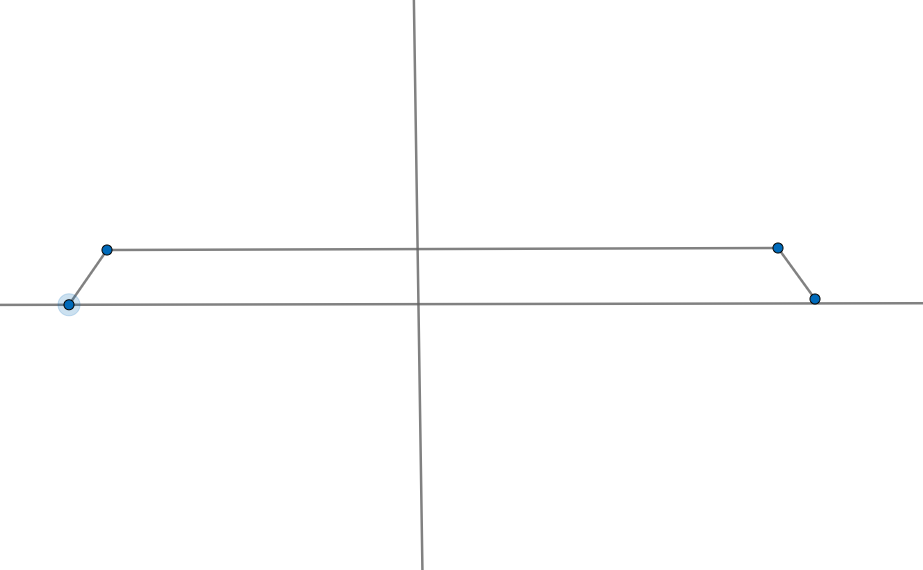
\includegraphics[width=2.5in]{spectralcluster/images/cheeger-counterexample.png}
\caption{
  The function $\rho_1$, a $1$-Lipschitz counterexample to Cheeger's inequality
  when $\alpha + \gamma > 2\beta$. 
  The height of the
  function is $\epsilon/2$, and the length of the supporting
  interval is roughly $\frac{2}{\epsilon}$.
 }
\label{fig:buser-counterexample}
\end{figure}

\begin{figure}[H]
\centering
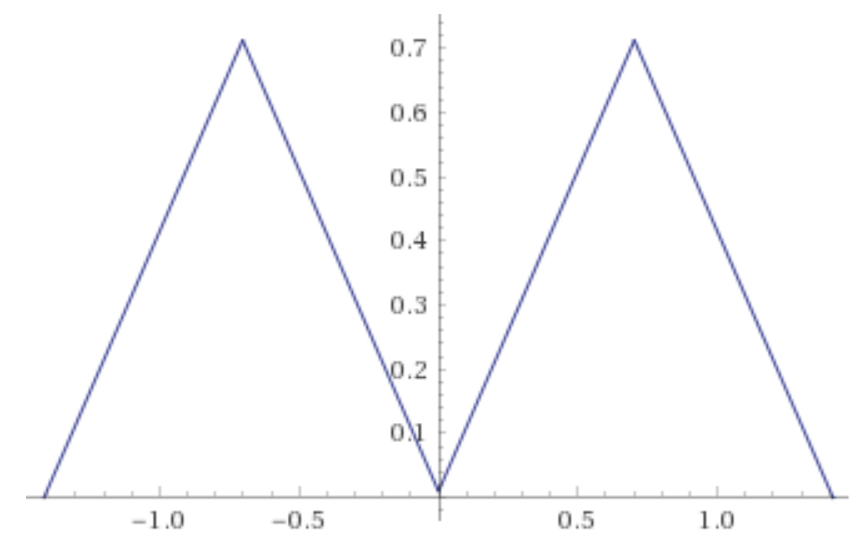
\includegraphics[width=2.5in]{spectralcluster/images/buser-counterexample.png}
\caption{
  The function $\rho_2$, a $1$-Lispchitz counterexample to Buser's inequality
  when $\gamma \geq 1$ and $ \gamma - 1 < \beta$.
 }
\label{fig:buser-counterexample}
\end{figure}


We will show that if $\alpha, \beta, \gamma$ satisfy $\alpha +
\gamma > 2\beta$, then the Cheeger inequality will fail for
$\rho_1$, and if $\gamma \geq 1$ and $\gamma - 1 < \beta$, then the Buser inequality
will fail for $\rho_2$.

In example $\rho_1$, let $\epsilon < 0.01$. The $(\alpha, \beta)$ isoperimetric constant
$\Phi$ is $O((1/\epsilon)^{\alpha - \beta - 1})$, and the eigenvalue
is $O((1/\epsilon)^{\alpha - \gamma - 2})$.  Therefore, the Cheeger
inequality will fail for some $\epsilon$ if $2 (\alpha - \beta - 1) > \alpha - \gamma -
2$, or $\alpha + \gamma > 2\beta$. This proves
Lemma~\ref{lem:cheeger-converse}.

In example $\rho_2$, let $\epsilon < 0.01$. The $(\alpha, \beta)$ isoperimetric constant
$\Phi$ is $O(\epsilon^{\beta})$. The eigenvalue
$\lambda_2$ is lower bounded by $O(\epsilon^{\gamma-1})$ when
$\gamma > 1$, and $\ln(1/\epsilon)$ when $\gamma =1$.
In either case, the Buser inequality will fail if $\gamma - 1 <
\beta$, proving Lemma~\ref{lem:buser-converse}.

We show details of our eigenvalue and isoperimetry calculations
in Appendix~\ref{app:examples}.


%!TEX root = ms.tex

\section{Buser Inequality for Probability Density Functions} \label{sec:buser}

In this section the theory of functions of bounded variation is used to
justify certain formal calculations. The key step is to define the geometric
quantities variationally.

\begin{definition}
  For a measurable set $A\subseteq \Re^d$ and $\rho:\Re^d \rightarrow
  \Re_{\geq 0}$ integrable define
  \begin{align*}
    \abs{A}_\alpha \coloneqq \int_A \rho^\alpha(x)\,dx.
  \end{align*}
\end{definition}

We define the weighted boundary area
variationally~\cite{betta2008weighted,parini2011introduction}.

\begin{definition}
\label{def:betaBdy}
For $\rho:\Re^d \rightarrow \Re_{\geq 0}$ integrable and $A\subseteq\Re^d$
the weighted perimeter of $A$ is
\begin{align*}
\abs{\boundary A}_\beta \coloneqq \sup\set{
\int_A \div(\rho^\beta (x) \phi(x))\,dx
\smid \phi\in C_c^1(\Re^d),\, \norm{\phi}_{\infty}\leq 1}.
\end{align*}
\end{definition}

\begin{remark}
  This definition corresponds to the intuitive definition of the
  boundary integral of $\rho^\beta$ when $\boundary A$ is sufficiently
  regular.  Specifically, if $A\subseteq\Re^d$ has smooth boundary
  and then,
  $$
  \abs{\boundary A}_\beta = \int_{\boundary A} \rho^\beta(x)\,d \mc H^{n-1}(x),
  $$
  where $\mc H^{n-1}$ denotes surface (Hausdorff) measure.
\end{remark}

\begin{definition}
  Let $A\subseteq\Re^d$ be a set of finite perimeter such that
  $\abs{A}_\alpha,\abs{\Re^d\setminus A}_\alpha >0$. The
  \textit{isoperimetric ratio} of the cut induced by $A$ is
\begin{align*}
\Phi(A) &\coloneqq \frac{\abs{\boundary A}_\beta}
{\min\left(\abs{A}_\alpha,\abs{\Re^d\setminus A}_\alpha\right)}
\end{align*}
and the \textit{isoperimetric constant} with weight $\rho$ is
\begin{align*}
  \Phi \coloneqq \inf_{A\subseteq \Re^d} \Phi(A).
\end{align*}
Here, $A$ is taken over sets of finite perimeter such that
$\abs{A}_\alpha,\abs{\Re^d \setminus A}_\alpha>0$.
\end{definition}

\subsection{Weighted Buser-type Inequality}

We now prove our weighted Buser-type inequality
Theorem~\ref{thm:Cheeger-Buser}. We state our result in terms of
general $(\alpha, \beta, \gamma)$.

\begin{theorem}
  \label{thm:buser_n}
  Let $\rho: \Re^d \to \Re_{\geq 0}$ be an $L$-Lipschitz function,
  $\lambda_2$ be a $(\alpha, \gamma)$-principal eigenvalue, and
  $\Phi$ the $(\alpha, \beta)$ isoperimetric cut.

  Then:
  \begin{align*}
    \lambda_2 \leq 3 \cdot 2^{\beta + 1} d \linf{\rho^{\gamma-\beta-1}}
    \max\left(L \Phi, 2^{\beta+1}\linf{\rho^{\alpha+1-\beta}} \Phi^2 \vph\right)
\end{align*}
\end{theorem}

We note that when setting $(\alpha, \beta, \gamma) = (1,2,3)$,
the above expression simplifies into:

\begin{align*}
  \lambda_2 \leq 24 d 
  \max\left(L \Phi, 8 \Phi^2 \vph\right).
\end{align*}

\subsection{Proof Strategy: Mollification by Disks of Radius
  Proportional to \texorpdfstring{$\rho$}{rho}}
To prove Theorem \ref{thm:buser_n}, for $A \subset \Re^d$ fixed, we
construct an approximation $u_\theta$ of the characteristic function,
$u$, of $A$ for which the numerator and denominator of the Rayleigh
quotient, $R(u_\theta)$, approximate respectively the numerator and
denominator of this expression.  Specifically, $u_\theta$ will
constructed as a mollification of $u$, Recall the following two
equivalent definitions of a mollification.  They are equivalent by the
change of variables $z = x-\theta \rho(x) y$.

\begin{equation} \label{eqn:utheta}
u_\theta(x) 
\coloneqq \int_{B(0,1)} \!\!\! u(x-\theta \rho(x) y) \phi(y) \, dy
= \int \! u(z) \phi_{\theta \rho(x)}(x-z) \, dz,
\quad \text{ where } \quad
\phi_{\eta}(z) 
= \frac{1}{\eta^d} \phi\left(\frac{z}{\eta}\right),
\end{equation}

with $\theta > 0$ a parameter to be chosen and $\phi:\Re^d \rightarrow
[0,\infty)$ a smooth radially symmetric function supported in the unit
open ball $B(0,1)=\{x \in \Re^d \;| \; |x| < 1\}$ with unit mass
$\int_{\Re^d} \phi = 1$. When $\rho$ is constant it follows from the
Tonelli theorem that $\lone{u_\theta} = \lone{u}$; when $\rho$ is not
constant the following lemma shows that the latter still bounds the
former.


\subsection{Key Technical Lemma: Bounding $L_1$ norm of a
  function with the $L_1$ norm of its
    mollification}\label{sec:key_lemma}
The following is our primary technical lemma, which roughly bounds the
$L_1$ norm of a mollified function $f$ by the $L_1$
norm of the original $f$. Here, the mollification radius is
determined by a function $\delta(x)$.
\begin{lemma} \label{lem:lonetheta} 

  Let
  $\delta:\RR^d\to\RR$ be Lipschitz continuous with Lipschitz constant
  $|\grad\delta(x)| \leq c < 1$ for almost every $x \in \bbR^d$. Let
  $\phi:\RR^d\to\RR_{\geq 0}$ be smooth, $\int_{\RR^d}\phi = 1$, and
  $\supp(\phi)\subseteq B(0,1)$.  Then
  \[
  \frac{1}{1+c}\norm{f}_{L^1}
  \leq \int_{\RR^d} \int_{B(0,1)} 
  \abs{f(x-\delta(x) y)}\phi(y)\,dy\,dx\leq
  \frac{1}{1-c}\norm{f}_{L^1},
  \qquad
  f \in L^1(\RR^d).
  \]
\end{lemma}

\begin{proof} (of Lemma~\ref{lem:lonetheta})
An application of Tonelli's theorem shows
\begin{align}
\int_{\RR^d} \int_{B(0,1)} \abs{f(x-\delta(x) y)}\phi(y)\,dy\,dx
=  \int_{B(0,1)}\phi(y)\int_{\RR^d} \abs{f(x-\delta(x)y)}\,dx\,dy.
\end{align}
Fix $y\in B(0,1)$ and consider the change of variables $z = x-\delta(x)y$. The
Jacobian of this mapping is $I - y \otimes \nabla \delta(x)$ which by Sylvester's determinant theorem has
determinant $1-y.\nabla \delta(x) > 0$. It follows that
\begin{align}
\int_{\RR^d} \int_{B(0,1)} 
\abs{f(x-\delta(x) y)}\phi(y)\,dy\,dx
=  \int_{B(0,1)}\phi(y)\int_{\RR^d} 
\frac{|f(z)|}{1-y.\nabla \delta(x)} \, dx \,dy,
\end{align}
and the lemma follows since $1-c \leq 1-y.\nabla \delta(x) \leq 1+c$.
\end{proof}
(Here, $a.b$ denotes the dot product between $a$ and $b$.)

We present the following simple corollaries, which is the primary
way our proof makes use of Lemma~\ref{lem:lonetheta}

\begin{corollary}\label{cor:lonetheta}
For any Lipschitz continuous function $\rho: \bbR^d \rightarrow \bbR^{\geq 0}$
with Lipschitz constant $L$ and any $\theta$ with $0 < \theta L < 1$, we have:
$$
\frac{1}{1+\theta L} \lone{\rho^\beta\nabla u}
\leq \int_{\bbR^d} \int_{B(0,1)} \rho^\beta ( x - \theta \rho(x) y)
  |\nabla u(x-\theta \rho(x)y)| \phi(y)\,dy\,dx
 \leq \frac{1}{1-\theta L} \lone{ \rho^\beta\nabla u},
$$
when $\rho^\beta |\nabla u| \in \Lone$.
\end{corollary}

\begin{proof} (of Corollary~\ref{cor:lonetheta}) Apply
  Lemma~\ref{lem:lonetheta} with $\delta(x) = \theta \rho(x)$, and
  $f(x) = \rho^\beta(x) \nabla u(x)$.
\end{proof}

This corollary will be used to bound the numerator of our
Rayleigh quotient.
Note that the expression
\[ \int_{\bbR^d} \int_{B(0,1)} \rho^\beta ( x - \theta \rho(x) y)
|\nabla u(x-\theta \rho(x)y)| \phi(y) dy dx
\]
is close to $\int_{\bbR^d} \rho^\beta(x) \nabla |u_\theta(x)| dx$ when
$\theta \leq \frac{1}{2L}$. This is the guiding intuition behind how
Corollary~\ref{cor:lonetheta} and Lemma~\ref{lem:lonetheta} will be
used, and will be formalized later in our proof of
Theorem~\ref{thm:buser_n}.

We present another simple corollary whose proof is equally
straightforward. This corollary will be used to bound the denominator,
and is a small generalization of Corollary~\ref{cor:lonetheta}. We
write down both corollaries anyhow, since this will make it easier to
interpret our bounds on the Rayleigh quotient.

\begin{corollary}\label{cor:lone-t-theta}
For any Lipschitz continuous function $\rho: \bbR^d \rightarrow \bbR^{\geq 0}$
with Lipschitz constant $L$, any $0 < t < 1$, and any $\theta$ with $0 < \theta L < 1$, we have:
$$
\frac{1}{1+\theta L} \lone{\rho^\beta \nabla u}
\leq \int_{\bbR^d} \int_{B(0,1)} \rho^\beta ( x - \theta t \rho(x) y)
|\nabla u(x-\theta t \rho(x)y)| \phi(y)\,dy\,dx
\leq \frac{1}{1-\theta L} \lone{ \rho^\beta \nabla u}
$$
\end{corollary}

\begin{proof} (of Corollary~\ref{cor:lone-t-theta})
    Apply Lemma~\ref{lem:lonetheta} with
    $\delta(x) = \theta t \rho(x)$, and $f(x) = \rho^\beta(x) \nabla u(x)$.
\end{proof}

A key technical step is to observe that the above two corollaries hold
when $u$ is a function of bounded variation provided the left and right
terms are interpreted as their variation. In particular, consider $A
\subset \Re^d$ with finite perimeter and let $u$ be the
characteristic function of $A$. ($u(x) = 1$ if $x \in A$ and zero
otherwise). Then there exists a sequence of functions
$\{u_n\}_{n=1}^\infty \subset C^\infty(\Re^d)$ with $u_n \rightarrow
u$ in $\Lone$ for which \cite{EvansMeasure15}
\begin{equation} \label{eqn:Aapprox}
\abs{\boundary A}_\beta
= \lim_{n \rightarrow \infty} \int_\Omega  \rho^\beta|\nabla u_n|
\eqqcolon  \int_\Omega  \rho^\beta|\nabla u|.
\end{equation}
Interchanging $A$ and $\Omega \setminus A$ if necessary, it follows that
$\Phi(A)$ defined in Definition \ref{def:betaBdy} can be written as
$$
\Phi(A) 
= \frac{\int_\Omega \rho^\beta |\nabla u|}{\int_\Omega \rho^\alpha u}
= \lim_{n\to\infty}\frac{\int_\Omega \rho^\beta\abs{\grad u_n}}{\int_\Omega\rho^\alpha \abs{u_n}}.
$$

Now we are ready to prove our main Theorem, which is the Buser
inequality for probability densities stated in
Theorem~\ref{thm:buser_n}.
\begin{proof} (of Theorem \ref{thm:buser_n})

Fix $A \subset \RR^d$ with $|A|_\alpha \leq |1|_\alpha / 2$ and let
$u(x) = \chi_A(x)$ be the characteristic function of $A$. Setting 
$\ubar$ to be the weighted average of $u$,
\[
\ubar 
= \frac{\int \rho^\alpha u}{\int \rho^\alpha}
= \frac{\int_A \rho^\alpha}{\int \rho^\alpha}
= \frac{|A|_\alpha}{|1|_\alpha} \in [0,1/2],
\qquad \text{ then } \qquad
\int \rho^\alpha (u-\ubar) = 0,
\]
and
  \begin{equation}\label{eqn:blah}
\lone{\rho^\alpha(u-\ubar)} 
= \int \rho^\alpha |u-\ubar| = 2 |A|_\alpha (1-\ubar)
= 2 \int \rho^\alpha |u-\ubar|^2.
  \end{equation}

Since $|A|_\alpha = \lonea{u}$ and $1-\ubar \in [0,1/2]$ it follows that

\begin{equation} \label{eqn:PhiA}
  (1/2) \frac{\lone{\rho^\beta \nabla u}}{\lone{\rho^\alpha(u-\ubar)}} 
  \leq \Phi(A) = \frac{\lone{\rho^\beta \nabla u}}{\lone{\rho^\alpha u}}
  \leq \frac{\lone{\rho^\beta \nabla u}}{\lone{\rho^\alpha(u-\ubar)}}.
\end{equation}

In the calculations below we omit the limiting argument with smooth
approximations of $u$ in equation \eqnref{:Aapprox} which justify
formula involving $\nabla u$. In particular, only the $\Lone$ norm
of $\rho^\beta |\nabla u|$ will appear in the estimates since this
has meaning while the $\Ltwo$ norm is undefined.

Next, let $u_\theta$ be the mollification of (an extension of) $u$
given by equation \eqnref{:utheta}. Then $u_\theta(x)$ is a local
average average of $u$ so $u_\theta(x) \geq 0$, $\linf{u_\theta} \leq
1$ and $\linf{u-u_\theta} \leq 1$.  Letting $L$ denote the Lipschitz
constant of $\rho$, the parameter $\theta$ will to be chosen 
less than $1/(2L)$ so that that Lemma \ref{lem:lonetheta} is applicable
with constant $c = 1/2$.

The remainder of the proof constructs an upper bound on the numerator
  $\int_{\bbR^d} \rho^\gamma |\nabla u_\theta|^2$ of the Rayleigh quotient
for $u_\theta - \ubar_\theta$ by $\lone{\rho^\beta \nabla u}$ and to
  lower bound the denominator $\int_{\bbR^d} \rho^\alpha (u_\theta -
\ubar_\theta)^2$ by $\lone{\rho^\alpha (u-\ubar)}$. The conclusion
of the theorem then follows from equation \eqnref{:PhiA}.

\subsection{Upper Bounding the Numerator}
To bound the $L^2$ norm in
  the numerator of the Rayleigh quotient by the $L^1$ norm in the
  numerator of the expression for $\Phi(A)$ it is necessary to obtain
  uniform bound on $\rho(x) \nabla u_\theta(x)$. 
  
  \begin{lemma} \label{lem:rep1}
  Let $u$ be any function, and let $u_{\theta}$ be defined as in
  Equation~\ref{eqn:utheta}. Let $\rho: \Re^d \to \Re_{\geq 0}$ be an
  $L$-Lipschitz function.
  \begin{align}
  \linf{\rho (x) \nabla u_\theta(x)}
    \leq \linf{u} \frac{d(2+3L)}{\theta}
  \end{align}
  \end{lemma}

  \begin{proof}
  In order to prove this lemma, we first need to get a handle on
  $\nabla u_\theta(x)$, which is the gradient of $u$ after
  mollification by $\theta$.

  We take the
  the second representation of $u_\theta$ in equation \eqnref{:utheta}
  to get
  \begin{align}
  \nabla u_\theta(x) 
  = \int_{\bbR^d} u(z) \left\{
    \frac{-d}{\theta \rho(x)} \phi_{\theta \rho}(x-z) \nabla \rho
    + \frac{1}{(\theta \rho(x))^{d+1}} 
    \left( I 
      + \nabla \rho(x) \otimes \frac{x-z}{\theta \rho(x)} \right)
    \nabla \phi \left(\frac{x-z}{\theta \rho(x)} \right) \right\}
    \, dz,
  \end{align}
  which is a consequence of the multivariable chain rule. Here,
  $v \otimes u$ refers to the outer product of $v$ and $u$.

  Multiplying by $\rho$ gives:
  \begin{align}
  \rho (x) \nabla u_\theta(x) 
  = \int_{\bbR^d} u(z) \left\{
    \frac{-d}{\theta} \phi_{\theta \rho(x)}(x-z) \nabla
    \rho(x)
    + \frac{1}{(\theta^{d+1} \rho(x)^{d})} 
    \left( I 
      + \nabla \rho(x) \otimes \frac{x-z}{\theta \rho(x)} \right)
    \nabla \phi \left(\frac{x-z}{\theta \rho(x)} \right) \right\} \, dz.
  \end{align}
  Now, we can bound the above equation by carefully bounding each
  part. We note:
  \begin{align} \label{eq:Cphi-calculation}
    & \int_{\bbR^d} \frac{1}{(\theta^{d+1} \rho(x)^d)} \nabla
    \phi\left(\frac{x-z}{\theta \rho(x)} \right) dz
    \\
    & = \int_{\bbR^d} \frac{1}{(\theta^{d+1} \rho(x)^d)} \nabla
    \phi\left(\frac{-z}{\theta \rho(x)} \right) dz
    \\
     & = \frac{1}{\theta} \int_{\bbR^d} \nabla \phi(-y) dy
  \end{align}
  where the last step follows by a simple change of variable.
  Here, we note that $\nabla \phi(y)$ is a vector, and the
  integral is over $\bbR^d$, which is how we eliminated
  $\frac{1}{(\theta \rho(x))^d}$ from the expression.

  Next, we examine the term: 
  \begin{align}
    I + \nabla \rho(x) \otimes \frac{x-z}{\theta \rho(x)}
  \end{align}
  Here, we aim to bound the operator norm of this matrix. Here,
  we note that 
  \[ |x - z| \leq \theta \rho(x) \]
  when 
  \[
    \nabla \phi\left(\frac{x-z}{\theta \rho(x)}\right) \not= 0
  \]
  and thus, when the latter equation holds, we can say:

  \[
    \left| \frac{x-z}{\theta \rho(x)}\right| < 1.
  \]
  Since $|\nabla \rho(x) < L|$, we now have:
  \begin{align}\label{eqn:num-matrix-norm-bound}
    |I + \nabla \rho(x) \otimes \frac{x-z}{\theta \rho(x)}|_2 <
    3/2
  \end{align}
  Combining Equation~\ref{eqn:num-matrix-norm-bound} Equation~\ref{eq:Cphi-calculation} to show:
  \begin{align}
    & \left | \int_{\bbR^d}
    \frac{1}{(\theta^{d+1} \phi(x)^{d})} \left( I + \nabla \rho(x) \otimes \frac{x-z}{\theta \rho(x)}
    \right) \nabla \phi \left( \frac{x-z}{\theta \rho(x)}
    \right) dz \right| 
    \\
    & \leq \frac{(1 + L)}{\theta} \int_{\bbR^d} |\nabla\phi(y) | dy,
  \end{align}
  where $L = \linf{\nabla \rho}$ is the Lipschitz constant for $\rho$. 
  We note that Section~\ref{sec:dimension-dep} shows that 
  \begin{align}
    \int_{\bbR^d} | \nabla \phi(y) dy| \leq 2d.
  \end{align}
  and therefore:
  \begin{align}
    & \left | \int_{\bbR^d}
    \frac{1}{(\theta^{d+1} \phi(x)^{d})} \left( I + \nabla \rho(x) \otimes \frac{x-z}{\theta \rho(x)}
    \right) \nabla \phi \left( \frac{x-z}{\theta \rho(x)}
    \right) dz \right| 
    \\ \label{eq:rho-grad-utheta-2}
    & \leq \frac{2d(1+L)}{\theta}
  \end{align}

  Now we turn our attention to the first term, which is:
  \begin{align}
    \int_{\bbR^d} \frac{-d}{\theta} \phi_{\theta \rho(x)}(x-z)
    \nabla\rho(x) dz
  \end{align}
  We note that 
  \[ 
    \int_{\bbR^d}\left| \phi_{\theta \rho(x)}(x-z)\right| dz
    = 1
  \]
  by our definition of $\phi$ (which was defined when we defined
      $u_\theta$). Combining this
  with $|\nabla \rho(x)| < L$, we get:
  \begin{align}
    & \int_{\bbR^d} \left | \frac{-d}{\theta} \phi_{\theta \rho(x)}(x-z)
    \nabla\rho(x) \right| dz
    \\ \label{eq:rho-grad-utheta-1}
    & < \frac{dL}{\theta}
  \end{align}
  Therefore, 
  \begin{align}
  &  \nonumber \left| \int_{\bbR^d} 
    \frac{-d}{\theta \rho(x)} \phi_{\theta \rho}(x-z) \nabla \rho
    + \frac{1}{(\theta \rho(x))^{d+1}} 
    \left( I 
      + \nabla \rho(x) \otimes \frac{x-z}{\theta \rho(x)} \right)
    \nabla \phi \left(\frac{x-z}{\theta \rho(x)} \right) \, dz
    \right|
    \\
    & \nonumber \leq \frac{d}{\theta}( L + 2(1+L)) 
    \\
  & = \frac{d(2+3L)}{\theta}.
  \label{eqn:}
  \end{align}
  where the first inequality comes from combining
  Equations~\ref{eq:rho-grad-utheta-2}
  and~\ref{eq:rho-grad-utheta-1}.

  This allows us to bound $\linf{\rho(x) \nabla u_{\theta}(x)}$:
  \begin{align}
  & \linf{\rho (x) \nabla u_\theta(x)}
  \\
  & = \linf{ \left| \int_{\bbR^d} u(z) \left\{
    \frac{-d}{\theta} \phi_{\theta \rho(x)}(x-z) \nabla
    \rho(x)
    + \frac{1}{(\theta^{d+1} \rho(x)^{d})} 
    \left( I 
      + \nabla \rho(x) \otimes \frac{x-z}{\theta \rho(x)} \right)
    \nabla \phi \left(\frac{x-z}{\theta \rho(x)} \right) \right\}
  \, dz \right| }
  \\
  & \leq \linf{u} \linf{ \int_{\bbR^d} \left| 
    \frac{-d}{\theta} \phi_{\theta \rho(x)}(x-z) \nabla
    \rho(x)
    + \frac{1}{(\theta^{d+1} \rho(x)^{d})} 
    \left( I 
      + \nabla \rho(x) \otimes \frac{x-z}{\theta \rho(x)} \right)
    \nabla \phi \left(\frac{x-z}{\theta \rho(x)} \right)
  \right| \, dz}
  \\
  & \leq \linf{u} \frac{d(2+3L)}{\theta}
  \end{align}
  where we make use of the fact that
    $\linf{ab} < \linf{a}\lone{b}.$
  This completes our proof.
  \end{proof}

  Next, we want an $L_1$ bound on $\rho^{\beta}(x) \nabla
  u_{\theta}(x)$.

  \begin{lemma} \label{lem:rep2}
  Let $u$ be any function, and let $u_{\theta}$ be defined as in
  Equation~\ref{eqn:utheta}. Let $\rho:\Re^d \to \Re_{\geq 0}$ be an
  $L$-Lipschitz function, and
  let $\theta L < 1/2$.

  Then:
  \begin{align}
      \lone{\rho^\beta(x) \nabla u_{\theta}(x)} \leq C_{\beta}
      \lone{\rho^\beta(x) \nabla u(x)}
  \end{align}
  \end{lemma}
  \begin{proof}
  First, we take the gradient 
  first representation of $u_\theta$
  in equation \eqnref{:utheta}. Using the chain rule gives us an
  alternate form for $\nabla u_\theta(x)$:

  \begin{align}
  \nabla u_\theta(x) 
  = \int_{\Re^d} 
  (I - \theta \nabla \rho \otimes y) \nabla u(x-\theta \rho y) \phi(y) \, dy,
  \end{align}
  so
  \begin{align}\label{eqn:rhoNablaUtheta}
  \rho^\beta(x) \nabla u_\theta(x) 
  = \int_{\Re^d} 
  (I - \theta \nabla \rho \otimes y)
  \frac{\rho^\beta(x)}{\rho^\beta(x-\theta \rho y)}
  \rho^\beta(x-\theta \rho y) \nabla u(x-\theta \rho y) \phi(y) \, dy.
  \end{align}

  The ratio in the integrand is bounded using the Lipschitz assumption
  on $\rho$ (and $|y| \leq 1$),
  \begin{equation} \label{eqn:rhoRatio}
    \frac{\rho(x)}{\rho(x-\theta \rho y)}
    \leq \frac{\rho(x)}{\rho(x) - L \theta \rho(x)}
    = \frac{1}{1 - L \theta} \leq 2,
    \qquad \text{ when } \theta < 1 / (2L).
  \end{equation}
  Note that 
  \begin{align} \label{eqn:matrix-norm} 
  \left\| I - \theta \nabla \rho \otimes y \right\|_2 \leq 3/2
  \end{align}
  where $\|M\|_2$ represents the $\ell^2$ matrix norm of $M$. This is
  because $|\nabla \rho(x) | \leq L$, and
  $\theta L < 1/2$, and $|y| \leq
  1$ every time $\phi(y) \not= 0$, and thus 
  \[ 
   \frac{I}{2} \preceq  I - \theta \nabla \rho \otimes y
   \preceq \frac{3I}{2}.
    \]
  
 Therefore, we can now apply Corollary~\ref{cor:lonetheta}
 to Equation~\eqnref{:rhoNablaUtheta} to show:
  \begin{align}
  \nonumber 
  & \lone{\rho^\beta(x) \nabla u_\theta(x)} 
  \\  \nonumber
  & \leq \|I - \theta \nabla \rho(x) \otimes y\|_2
  \cdot \max_x\left(\frac{\rho(x)}{\rho(x - \theta \rho
        y)}\right) \cdot
  \int_{\bbR^d} \left| \int_{\bbR^d} \rho^{\beta}(x - \theta \rho y) \nabla u(x - \theta \rho y)
    \phi(y) dy \right|
  \\ \nonumber 
  & \leq 3 \cdot 2^{\beta - 1} \int_{\bbR^d} \rho^\beta(x -
      \theta \rho(x) y) \nabla u (x - \theta \rho (x) y 
  \\ \nonumber
  & 
  \leq 3 \cdot 2^\beta \lone{\rho^\beta \nabla u},
  \qquad \text{ when } \theta < 1 / (2L).
  \end{align}
  here, the first inequality comes from the equation $\lone{abc}
  \leq \linf{a}\linf{b}\lone{c}$, the second inequality comes
  from Equations~\ref{eqn:rhoRatio} and~\ref{eqn:matrix-norm}, and the
  third inequality comes
  from Corollary~\ref{cor:lonetheta} assuming $\theta L \leq
  1/2$. 
  \end{proof}

  \begin{lemma}\label{lem:num}
  For any $L$-Lipschitz distribution $\rho$, any function $u$, and any $\theta$ such that $\theta L <
  1/2$:

  \begin{align}
  \int_{\bbR^d} \rho^\gamma |\nabla u_\theta|^2
  \leq  C_\beta \linf{\rho^{\gamma-\beta-1}} \frac{d(2+3L)}{\theta} 
  \linf{u} \lone{\rho^\beta \nabla u},
  \end{align}
  \end{lemma}

  \begin{proof}
  Combining the two estimates from Lemma~\ref{lem:rep1}
  and~\ref{lem:rep2} gives an upper bound for the Rayleigh
  quotient 
  \begin{align}
  \int_{\bbR^d} \rho^\gamma |\nabla u_\theta|^2
  = \int_{\bbR^d} \rho^{\gamma-\beta-1} \,
  \rho |\nabla u_\theta| \, \rho^\beta |\nabla u_\theta|
  \leq 3 \cdot 2^{\beta + 1} \linf{\rho^{\gamma-\beta-1}} \frac{d(2+3L)}{\theta} 
  \linf{u} \lone{\rho^\beta \nabla u},
  \end{align}
  \end{proof}

  We note that in the case where $\gamma = \beta + 1$, and if $u$ is a step
  function, the expression would
  simplify to:
  \[ \int_{\bbR^d}
  |\rho^{\gamma} |\nabla u_\theta|^2
  \leq 3 \cdot 2^{\beta + 1} \frac{d(2+3L)}{\theta} 
  \linf{u} \lone{\rho^\beta \nabla u},
  \]

\subsection{Lower Bound on the Denominator}
Let $\ubar$ and
  $\ubar_\theta$ be the $\rho^\alpha$--weighted averages of $u$ and
  $u_\theta$. For any function $f$, let $\ltwoa{f}$ denote the $L^2$ norm of $\rho^\alpha
  f$, and let $\lone{f}$ denote the $L^1$ norm of $\rho^\alpha f$ for
  functions $f$ where these two quantities are well defined.
  Our core lemma is a bound on $\ltwoa{u_\theta-\ubar_\theta}$ in
  terms of $l_1$ and weighted $l_1$ norms of $\nabla u$ and $u -
  \ubar$ respectively.
  \begin{lemma}\label{lem:denom}
  Let $\rho$ be an $L$-Lipschitz function $\rho: \Re^d \to
  \Re_{\geq 0}$, and let $\theta$ be such
  that $\theta L < 1/2$.
  Let $u$ be an indicator function of a set $A$ with finite
  $\beta$-perimeter. Let $\ubar$ be defined as $\ubar(x):=u(x) - \int u(y) dy$
    $u_\theta$ be defined as in Equation~\ref{eqn:utheta}, and
    $\ubar_\theta$ be defined as $\ubar_\theta(x) := u_\theta(x)
    - \int
    u_\theta(y) dy$.
    Then:
  \begin{align}
  \ltwoa{u_\theta - \ubar_\theta}^2
  \geq (1/4) \lonea{u-\ubar} 
  - C(\beta) \theta \linf{\rho^{\alpha+1-\beta}} \lone{\rho^\beta \nabla u},
  \qquad \text{ when } \theta < 1 / (2L).
  \end{align}
  \end{lemma}

  Note that when $\alpha + 1 = \beta$, as is true when $(\alpha,
      \beta, \gamma) = (1,2,3)$, the inequality in
  Lemma~\ref{lem:denom} becomes:

  \[
  \ltwoa{u_\theta - \ubar_\theta}^2
  \geq (1/4) \lonea{u-\ubar} 
  - C(\beta) \theta \lone{\rho^\beta \nabla u},
  \qquad \text{ when } \theta < 1 / (2L).
  \]
  The estimate in Lemma~\ref{lem:denom} will be combined with the
  estimate in Lemma~\ref{lem:num} to prove
  Theorem~\ref{thm:buser_n}
  in Section~\ref{sec:rayleigh-bound}.


  \begin{proof} The key to this proof is to upper bound the
  quantity $\ltwoa{u_\theta - \ubar_\theta}$ with the expression
  appearing in Corollary~\ref{cor:lone-t-theta}. We will do so by
  a series of inequalities, application of the fundamental
  theorem of calculus, and more.

  Using the property that subtracting the average from a
  function reduces the $L^2$ norm it follows that
  \begin{align}
  \nonumber
  & \ltwoa{u_\theta - \ubar_\theta}
  \\
    \nonumber
  & \geq \ltwoa{u-\ubar} - \ltwoa{u_\theta - u - (\ubar_\theta-\ubar)}
  \\
    \nonumber
  &\geq \ltwoa{u-\ubar} - \ltwoa{u_\theta - u}.
  \end{align}
  If $a \geq b-c$ then $a^2 \geq b^2/2 - c^2$, so a lower bound for
  the denominator of the Rayleigh quotient
  \begin{align} \label{eqn:utmu}
    & \ltwoa{u_\theta - \ubar_\theta}^2
    \\
    \nonumber
    &\geq (1/2) \ltwoa{u-\ubar}^2 - \ltwoa{u_\theta - u}^2
    \\
    \nonumber
    & \geq (1/4) \lonea{u-\ubar} - \lonea{u_\theta - u},
  \end{align}
  where the identity $\ltwoa{u-\ubar}^2 = \lonea{u-\ubar}/2$ from
  Equation~\ref{eqn:blah}, and the bound
  $\linf{u_\theta - u} \leq 1$, were used in the last step.

  It remains to estimate the difference $\lonea{u_\theta - u}$. To
  do this, we use the multivariable fundamental
  theorem of calculus to write
  \begin{eqnarray*}
    u_\theta(x) - u(x)
    &=& \int (u(x - \theta \rho y) - u(x)) \phi(y) \, dy \\
    &=& \int \! \int_0^1
    -\theta \rho(x) \nabla u(x - t \theta \rho(x) y).y \phi(y) \, dt \, dy \\
    &=& \int \! \int_0^1
    \frac{-\theta \rho(x)}{\rho^\beta(x-t\theta \rho(x) y)} 
    \rho^\beta(x - t\theta \rho(x) y) \nabla u(x - t \theta
        \rho(x) y).y \phi(y) \, dt \, dy,
  \end{eqnarray*}
  where the first and second equalities came from application of
  the multivariable fundamental theorem of calculus, and the last
  equation is straightforward. This tells us that:
  \begin{align}
  \notag
  & \rho^{\alpha}(x) ( u_\theta \rho(x) - u(x) )
  \\
  \notag
  & = \int \! \int_0^1
  \frac{-\theta \rho^{\alpha+1}(x)}{\rho^\beta(x-t\theta \rho y)} 
  \rho^\beta(x - t\theta \rho(x) y) 
  \nabla u(x - t \theta \rho(x) y).y \phi(y) \, dt \, dy.
  \\
    \label{eqn:utheta-l1-alpha}
  &= \int \! \int_0^1
  \frac{\rho^\beta(x)}{\rho^\beta (x- t \theta \rho(x)y)}
  \frac{-\theta \rho^{\alpha+1}(x)}{\rho^\beta(x)}
  \rho^{\beta}(x - t \theta \rho(x) y )
  \nabla u(x - t \theta \rho(x) y).y \phi(y) \, dt \, dy.
  \end{align}
  Equation \eqnref{:rhoRatio} bounds the ratio $\rho(x)/ \rho(x -
    t\theta \rho(x) y)$ as less than $2$ when $\theta L < 1/2$,
  so Equation~\eqnref{:utheta-l1-alpha} is always less than or
  equal to:
  \begin{align}
  \int \! \int_0^1
  2^{\beta}
  \frac{-\theta \rho^{\alpha+1}(x)}{\rho^\beta(x)}
  \rho^{\beta}(x - t \theta \rho(x) y )
  \nabla u(x - t \theta \rho(x) y).y \phi(y) \, dy \, dt.
  \end{align}

  An application of Corollary \ref{cor:lone-t-theta} then shows
  \begin{align}
  & \int \! \int_0^1
  2^{\beta}
  \frac{-\theta \rho^{\alpha+1}(x)}{\rho^\beta(x)}
  \rho^{\beta}(x - t \theta \rho(x) y )
  \nabla u(x - t \theta \rho(x) y).y \phi(y) \, dy \, dt.
  \\
  & \leq \int \! \int_0^1
  2^{\beta}
  \frac{-\theta \rho^{\alpha+1}(x)}{\rho^\beta(x)}
  \rho^{\beta}(x - t \theta \rho(x) y ) \ 
  \left|\nabla u(x - t \theta \rho(x) y) \phi(y)\right| \, dy \, dt.
  \\
  &
  \leq 2^{\beta+1} \linf{\rho^{\alpha+1-\beta}} \theta
  \int \! \int_0^1
  \rho^{\beta}(x - t \theta \rho(x) y ) \ 
  \left|\nabla u(x - t \theta \rho(x) y) \phi(y)\right| \, dy \, dt.
  \qquad \text{ when } \theta < 1 / (2L).
  \\
  &
  \leq 2^{\beta+1} \linf{\rho^{\alpha+1-\beta}} \theta \lone{\rho^\beta \nabla u}
  \end{align}
  where the last inequality follows from
  Corollary~\ref{cor:lone-t-theta}.

  Using this estimate in \eqnref{:utmu} gives a lower bound on the
  denominator of the Rayleigh quotient,
  \begin{align}
  \ltwoa{u_\theta - \ubar_\theta}^2
  \geq (1/4) \lonea{u-\ubar} 
  - 2^{\beta+1} \theta \linf{\rho^{\alpha+1-\beta}} \lone{\rho^\beta \nabla u},
  \qquad \text{ when } \theta < 1 / (2L).
  \end{align}
  as desired.
  \end{proof}

  \subsection{Bounding the Rayleigh
    Quotient (Proof of Theorem~\ref{thm:buser_n})}\label{sec:rayleigh-bound}
  Combining Lemmas~\ref{lem:num} and Lemmas~\ref{lem:denom}
  provides an upper bound for the Rayleigh quotient of $u_\theta - \ubar_\theta$,
  \begin{eqnarray*}
    \lambda_2 
    &\leq& \frac{\int_{\bbR^d} \rho^\gamma |\nabla u_\theta|^2}
    {\int_{\bbR^d} \rho^\alpha (u_\theta - \ubar_\theta)^2} \\
    &\leq&  \frac{d \cdot 3 \cdot 2^{\beta}}{\theta}
    \frac{\linf{\rho^{\gamma-\beta-1}} (2+3L) \lone{\rho^\beta \nabla u}}
    {\lonea{u-\ubar} 
      - 2^{\beta+1} \theta \linf{\rho^{\alpha+1-\beta}} \lone{\rho^\beta \nabla u}} \\
    &\leq&  \frac{d \cdot 3 \cdot 2^{\beta}}{\theta}
    \frac{\linf{\rho^{\gamma-\beta-1}} (2+3L)}
    {1 - 2^{\beta + 1} \theta \linf{\rho^{\alpha+1-\beta}} \Phi(A)} \Phi(A).
  \end{eqnarray*}
  Selecting $\theta = (1/2)
  \min\left(1/\left(2^{\beta+1}\linf{\rho^{\alpha+1-\beta}}
        \Phi(A)\right), 1/L
  \right)$ shows
  \[
  \lambda_2 \leq 2 d \cdot 3 \cdot 2^{\beta}
\linf{\rho^{\gamma-\beta-1}}(2+3L) 
  \max\left(L \Phi(A), 2^{\beta+1}\linf{\rho^{\alpha+1-\beta}} \Phi(A)^2 \vph\right).
  \]
  When $\gamma = (1,2,3)$, this simplifies into:
  \[
  \lambda_2 \leq 12(2+3L) d
  \max\left(L \Phi(A), 8 \Phi(A)^2 \vph\right).
  \]
  We note that, via the work shown in
  Section~\ref{sec:scaling},  we can strengthen our inequality
  to:
  \[
  \lambda_2 \leq 24 d
  \max\left(L \Phi(A), 8 \Phi(A)^2 \vph\right).
  \]

  \qedhere


\subsection{Gradient of Mollifier}\label{sec:dimension-dep}
Let $\phi$ be a standard mollifier i.e. $\phi\in C_c^\infty(\RR^d)$
is a function from $\RR^d\to [0,\infty)$ satisfying $\int_{\RR^d}
  \phi\,dx = 1$ and $\supp(\phi)\subseteq B(0,1)$.  We will define
  $\phi$ by its profile. Namely, let $\phihat(r):[0,\infty)
    \rightarrow [0,1]$ be a fixed monotone decreasing profile with
    $\phihat(0)=1$, $0 < \phihat(r) < 1$ for $0 < r < 1$, and
    $\phihat(r) = 0$ for $r \geq 1$. Then define $\phi:\Re^d
    \rightarrow \Re$ by $\phi(x) = c \phihat(|x|)$ with $c > 0$ chosen
    so that $\int_{\Re^d} \phi(x) \, dx = 1$; that is,

\[
1 = \int_{\Re^d} \phi(x) \, dx
= c |S^{d-1}| \int_0^1 \phihat(r) r^{d-1} \, dr
\qquad \Rightarrow \qquad
c = \frac{1}{|S^{d-1}| \int_0^1 \phihat(r) r^{d-1} \, dr},
\]

where $|S^{d-1}|$ is the $(d-1)$--area of the unit sphere in $\Re^d$.
We claim the $L_1$ norm of the gradient of $\nabla \phi(x)$ is linear in $d$.
\begin{lemma}\label{lem:molli}
  \[
  \int_{\Re^d} |\nabla \phi(x)| \, dx   
\leq (d-1) \left( \frac{d 2^d}{\phihat(1/2)} \right)^{1/(d-1)}
\stackrel{d \rightarrow \infty}{\longrightarrow} 2(d-1).
\]
For the classic mollifier $\phihat(r)=\exp(-1/(1-r^2))$ we get
  \[
  \int_{\Re^d} |\nabla \phi(x)| \, dx  \leq 2d.
\]
\end{lemma}

From the formula $\nabla \phi(x) = c \phihat'(|x|) (x/|x|)$ we compute
\begin{eqnarray*}
\int_{\Re^d} |\nabla \phi(x)| \, dx
&=& c |S^{d-1}| \int_0^1 |\phihat'(r)| r^{d-1} \, dr \\
&=& c |S^{d-1}| \int_0^1 -\phihat'(r) r^{d-1} \, dr \\
&=& c |S^{d-1}| \int_0^1 \phihat(r) (d-1) r^{d-2} \, dr \\
&=& (d-1) \frac{\int_0^1 \phihat(r) r^{d-2} \, dr}
{\int_0^1 \phihat(r) r^{d-1} \, dr}.
\end{eqnarray*}
To estimate the numerator use Holder's inequality: for
$1 \leq s, s' \leq \infty$ with $1/s + 1/s' = 1$ 
$$
\int f g 
\leq \left(\int |f|^s \right)^{1/s} \left(\int |g|^{s'} \right)^{1/s'}.
$$
Set $s = (d-1)/(d-2)$ and $s' = d-1$ to get
$$
\int_0^1 \phihat(r) r^{d-2} \, dr
= \int_0^1 \phihat(r)^{1/s} r^{d-2} \times \phihat(r)^{1/s'}  \, dr
\leq \left(\int_0^1 \phihat(r) r^{d-1} \, dr \right)^{1/s}
\left(\int_0^1 \phihat(r) \, dr \right)^{1/s'}.
$$
It follows that
\begin{equation}\label{eq:molli0}
\int_{\Re^d} |\nabla \phi(x)| \, dx
\leq (d-1) \left( \frac{\int_0^1 \phihat(r) \, dr}
{\int_0^1 \phihat(r) r^{d-1} \, dr} \right)^{1/(d-1)}.
\end{equation}
Since $0 \leq \phihat(r) \leq 1$ we can bound the numerator
by $1$, and since $\phihat(r)$ is monotone decreasing we have
$\phihat(r) \geq \phihat(1/2)$ on $(0,1/2)$, so 
\begin{equation}\label{eq:molli}
\int_{\Re^d} |\nabla \phi(x)| \, dx
\leq (d-1)
\left( \frac{1}{\phihat(1/2) \int_0^{1/2} r^{d-1} \, dr} \right)^{1/(d-1)} 
\leq (d-1) \left( \frac{d 2^d}{\phihat(1/2)} \right)^{1/(d-1)}
\stackrel{d \rightarrow \infty}{\longrightarrow} 2(d-1).
\end{equation}

It will be convenient to write equation~\ref{eq:molli} as a simple
inequality. Observer that
\[
 \left( \frac{d 2^d}{\phihat(1/2)} \right)^{1/(d-1)}
\]
is monotone decreasing. We now pick the classic
$\phihat(r) = \exp(-1/(1-r^2))$ we have $\phihat(1/2) \geq 1/4$ and if
$d \geq 5$ the right hand side of equation (\ref{eq:molli} is bounded
by $2d$. If $d < 5$ explicit computations of the integrals shows the
right hand side of equation (\ref{eq:molli0} is bounded by $2d$.







\end{proof}



\subsection{Scaling}\label{sec:scaling}

In this section we show that if one scales the density function $\rho$ then
the isoperimetric value $\Phi(A)$ and the Rayleigh quotient $R(u)$
scale nicely. More formally Let $A \subset \Omega \subseteq
\Re^d$, $\rho$ a density function over a domain $\Omega$, and
$u$ an arbitrary differentiable  function over $\Omega$.

Consider the transformation
$\xhat = \ell x$ with $\ell > 0$ which maps $\Omega$ to the domain
$\Omegahat = \{\ell x \sst x \in \Omega\}$. Given $u:\Omega \rightarrow
\Re$, we define $\uhat: \Omegahat \rightarrow \Re$ by $\uhat(\xhat) =
u(x)$. We will future scale $\rho$ by $\alpha \rhohat(\xhat) = \ell \, \rho(x)$ where
$\alpha > 0$.

\begin{theorem}\label{thm:scaling}
  When scaling by $\alpha$ and $\ell$ then
  \[   \Phi(A) = \alpha \Phihat(\Ahat) \] and
  \[  R(u)  = \alpha^2 \Rhat(\uhat) \quad \text{and thus} \quad\lambda_2 = \alpha^2 \hat{\lambda}_2\].
\end{theorem}

We will use this scaling theorem to improve the bounds
of theorem~\ref{thm:buser_n}. 

That is, if we have a density function $\rho$ over
a domain $\Omega$ the isoperimetric number that the fundamental eigenvalue only
change as a function  of the scaling.  Thus the optimal cut and eigenvector are
unchanged by scaling up to the transformation.

%% Given a domain $\Omega \subset \Re^d$, consider the transformation
%% $\xhat = \ell x$ with $\ell > 0$ which maps $\Omega$ to the domain
%% $\Omegahat = \{\ell x \sst x \in \Omega\}$. If $u:\Omega \rightarrow
%% \Re$, define $\uhat: \Omegahat \rightarrow \Re$ by $\uhat(\xhat) =
%% u(x)$.

If $u$ and $l$ are as defined above then we get the simple but basic identity. 
Suppose that $u: \R \rightarrow \R$ then: \[
\dbydp{u}{x} 
= \dbydp{\uhat}{\xhat} \dbydp{\xhat}{x}
= \dbydp{\uhat}{\xhat} \ell,
\qquad \text{ in general we get } \qquad
|\nabla u(x)| = \ell |\hat{\nabla} \uhat(\xhat)|.
\]

In the case of $\rho:\Omega \rightarrow (0,\infty)$, where
$\rhohat: \Omegahat \rightarrow (0,\infty)$ is defined by
$ \alpha \rhohat(\xhat) = \ell \, \rho(x)$ we get that
\[
|\nabla \rho(x)| = \alpha |\hat{\nabla} \rhohat(\xhat)|.
\]

It follows that $L_{\rhohat}$ and $L_\rho$, the Lipschitz constants
for $\rhohat$ and $\rho$,  satisfy $L_{\rhohat} = (1/\alpha) L_\rho$.

\begin{itemize}
\item
  Since $d\xhat = \ell^{d} \, dx$ we have
  \[
  \int_\Omega \rho \, dx = \frac{\alpha}{\ell^{d+1}} \int_{\Omegahat} \rhohat \, d\xhat, 
  \]
  %% so it is always possible to choose a scaling to get $\int_{\Omegahat}
  %% \rhohat = 1$.

\item
  If $A \subset \Omega$ and $\Ahat = \ell A \subset \Omegahat$,
  let $f_A(x) = 1$ if $x \in A$ and zero otherwise, and similarly
  $f_{\Ahat} = 1$ if $\xhat \in \Ahat$ and zero otherwise. We next perform
  a set of standard integral calculations.
  \begin{align}
  \int_\Omega \rho^2 |\nabla f_A| \, dx &=
  \int_{\Omegahat} (\frac{\alpha}{\ell})^2 \rhohat^2 \ell |\hat{\nabla} f_{\Ahat}|
  \, \frac{1}{\ell^d} d\xhat \label{eq:subsitution}\\
  &= \frac{\alpha^2}{\ell^{d+1}} \int_{\Omegahat} \rhohat^2  |\hat{\nabla} f_{\Ahat}|
  \, d\xhat \label{eq:integral1}
  \end{align}

  Equation~\ref{eq:subsitution} follows by making the substitutions:
  \[ \rho(x) = (\frac{\alpha}{\ell}) \rhohat(\xhat) \quad
  |\nabla f_A| = \ell |\hat{\nabla} f_{\Ahat}| \quad
  dx =  \frac{1}{\ell^d} d\xhat
  \]
  Observing the $f_A(x) = f_{\Ahat}(\xhat)$ we get the following identity.
\begin{equation}\label{eq:integral2}
 \int_\Omega \rho f_A \, dx
 = \int_{\Omegahat} \frac{\alpha}{\ell}  \rhohat f_{\Ahat} \frac{1}{\ell^d} \, d\xhat
   = \frac{\alpha}{\ell^{d+1}} \int_{\Omegahat} \rhohat f_{\uhat} \, d\xhat
\end{equation}

Combining equation~\ref{eq:integral1} and equation~\ref{eq:integral2}
we get that:

\begin{equation}
  \Phi(A) = \alpha \Phihat(\Ahat)
\end{equation}

\item
  We next do a similar calculation for the Rayleigh quotient.
  If $u:\Omega \rightarrow \Re$ and $\uhat(\xhat) = u(x)$, 
  the Rayleigh quotients can be computed as follows,
  \[
  \int_\Omega \rho^3 |\nabla u|^2 \, dx
  = \int_{\Omegahat} (\frac{\alpha}{\ell})^3 \rhohat^3
  \ell^2 |\hat{\nabla} \uhat|^2 \, \frac{1}{\ell^d} d\xhat
    = \frac{\alpha^3}{\ell^{d+1}} \int_{\Omegahat} \rhohat^3 |\hat{\nabla} \uhat|^2 \, d\xhat
 \]

\[
\int_\Omega \rho u^2 \, dx
= \int_{\Omegahat} \frac{\alpha}{\ell} \rhohat \uhat^2 \frac{1}{\ell^d} \, dx
= \frac{\alpha}{\ell^{d+1}} \int_{\Omegahat} \rhohat \uhat^2 \, dx
\]
Thus \[  R(u)  = \alpha^2 \Rhat(\uhat) \].
\end{itemize}

We next use our scaling result in the $(1,2,3)$ case
to our Buser-type bound, Theorem~\ref{thm:buser_n}.
Theorem~\ref{thm:buser_n} states that the following hold:

\begin{align}\label{eq:simple123}
  \lambda_2 \leq 24 d (1+L) 
  \max\left(L \Phi(A), 12 \Phi(A)^2 \vph\right).
\end{align}

We now make substitutions into equation~\ref{eq:simple123}
from Theorem~\ref{thm:scaling} and its proof for some parameter $\alpha$ to be determined.


\begin{align*}
  \lambda_2 = \alpha^2 \hat{\lambda}_2 &\leq  \alpha^2  24 d (1+\hat{L}) 
  \max\left(\hat{L} \Phihat(\Ahat), 12 \Phihat(\Ahat)^2 \vph\right) \\
  &=  \alpha^2  24 d (1+ (L/\alpha))
  \max\left((L/\alpha) (\Phi(A)/\alpha), 12 (\Phi(A)/\alpha)^2 \vph\right) \\
  &=  24 d (1+ (L/\alpha))
  \max\left(L \Phi(A), 12 \Phi(A)^2 \vph\right) \\
  &=  24 d \max\left(L \Phi(A), 12 \Phi(A)^2 \vph\right)
\end{align*}
where the last line holds when taking $\alpha$ to infinity.

Thus we get that $\lambda_2$ only depends linear in the dimension and  the Lipschitz constant:

\begin{corollary}\label{cor:strongBuser}
  \[
  \lambda_2 \leq  24 d \max\left(L \Phi, 12 \Phi^2 \vph\right)
  \]
\end{corollary}





\section{Cheeger Inequality for Probability Density Functions}\label{sec:cheeger}

In this section, we prove the Cheeger inequality from
Theorem~\ref{thm:Cheeger-Buser}. That is a weighted Cheeger inequality in higher dimensions.
This is the easier to prove than Buser's inequality, which
contrasts with what happens in the graph case (the graph Buser
    inequality is trivial).

For a simplified proof of the Cheeger inequality for distributions
in one-dimension, see Appendix~\ref{sec:one_dim}.

As we will see from simple counterexamples in
Section~\ref{sec:examples}, the Cheeger-direction does not
hold for all setting of $(\alpha,\beta,\gamma)$. The proof we give is
requires fewer assumptions than the Buser inequality for
probability densities. One, the Cheeger inequality is
independent of the Lipschitz constant of $\rho$ and two, the proof
also holds when $\rho$ is supported on a set
$\Omega \subset \mathbb{R}^d$.

The proof is almost identical to the proof in one dimension and only a
slight modification of standard proofs The only change in the proof is
replacing the change of variables formula with a co-area formula.  Let
$\rho:\Omega \to \RR_>$ be an Lipschitz density function that is
$(\alpha,\beta,\gamma)$-integrable over an open set $\Omega \subseteq
\RR^d$.  Note a stronger hypothesis  on $\Omega$ is that it is the support of
$\rho$ when  $\rho:\RR^d \to \RR_\leq$. 

\begin{theorem}
\label{thm:cheeger_n}
Let $\rho:{\Omega}\to\RR_{>0}$ be a Lipschitz function. Then,
\begin{align*}
\Phi^2 \leq 4 \norm{\rho^{\beta - \frac{\alpha+\gamma}{2}}}^2_\infty \lambda_2.
\end{align*}
In particular, when $(\alpha,\beta,\gamma) = (1,2,3)$ we have
\begin{align*}
\Phi^{2} \leq 4\lambda_2.
\end{align*}
\end{theorem}
Here, $\Phi$ is the optimal $(\alpha,\beta)$-sparsity of a cut
through $\rho$. We note that we can say something a little stronger:
\begin{theorem}
\label{thm:cheeger-sweep}
Let $\rho:{\Omega}\to\RR_{>0}$ be a Lipschitz function. 
Let $\Phi_{(\alpha,\beta,\gamma)}$ be the $(\alpha,\beta)$
sparsity of the $(\alpha, \gamma)$ spectral sweep cut. If $\alpha = \beta-1 = \gamma-2$,  then:
\begin{align*}
\Phi_{(\alpha, \beta, \gamma)}^2 \leq 4 \lambda_2
\end{align*}
\end{theorem}
\begin{proof} (of both theorems): 
Let $w\in W^{1,2}$, functions whose gradient is square integrable, nonzero with $\int_\Omega \rho^\alpha w\,dx = 0$. Let $v = w+a1$ where $a$ is chosen such that $\abs{\set{v<0}}_\alpha = \abs{\set{v>0}}$. Note that
\begin{align*}
R(w) &= \frac{\int_\Omega \rho^\gamma \abs{\grad w}^2\,dx}{\int_\Omega \rho^\alpha w^2\,dx}\\
&\geq \frac{\int_\Omega \rho^\gamma \abs{\grad w}^2\,dx}{\int_\Omega \rho^\alpha w^2\,dx+ a^2\abs{\Omega}_\alpha}\\
&= R(v).
\end{align*}
Without loss of generality, the function $u = \max(v,0)$ satisfies $R(u)\leq R(v)$.

Let $\Omega_0 = \set{v>0}$. Let $g = u^2$. Noting that $\grad g = 2u\grad u$ a.e., we can apply Cauchy-Schwarz to obtain
\begin{align*}
\int_{\Omega_0}\rho^\beta \abs{\grad g}\,dx &= 2\int_{\Omega_0}\rho^\beta \abs{u}\abs{\grad u}\,dx\\
&\leq 2 \sqrt{\int_{\Omega_0} \rho^{2\beta - \alpha} \abs{\grad u}^2\,dx}\sqrt{\int_{\Omega_0} \rho^{\alpha} u^2\,dx}\\
&\leq 2 \norm{\rho^{\beta - \frac{\alpha+\gamma}{2}}}_\infty \sqrt{\int_{\Omega_0} \rho^\gamma \abs{\grad u}^2\,dx}\sqrt{\int_{\Omega_0} \rho^{\alpha} u^2\,dx}.
\end{align*}
Then, dividing by $\int_{\Omega_0} \rho^\alpha g\,dx$, we have
\begin{align*}
\frac{\int_{\Omega_0} \rho^\beta \abs{\grad g}\,dx}{\int_{\Omega_0} \rho^\alpha g\,dx} &\leq2 \norm{\rho^{\beta - \frac{\alpha+\gamma}{2}}}_\infty \sqrt{R(w)}.
\end{align*}
Let $A_t = \set{g>t}$. Then, by the weighted co-area formula,
\begin{align*}
\int_{\Omega_0} \rho^\beta \abs{\grad g}\,dx = \int_0^\infty \abs{\boundary A_t}_\beta\,dt.
\end{align*}
Writing $g(x) = \int_0^{g(x)} 1 \,dt$ and applying Tonelli's theorem, we rewrite the denominator
\begin{align*}
\int_{\Omega_0} \rho^\alpha g\,dx = \int_{0}^\infty \abs{A_t}_\alpha\,dt.
\end{align*}
Thus, by averaging, there exists some $t^*$ such that
\begin{align*}
\Phi &\leq \Phi(A_{t^*})\\
&\leq \frac{\int_{\Omega_0} \rho^\beta \abs{\grad g}\,dx}{\int_{\Omega_0} \rho^\alpha g\,dx}\\
&\leq2 \norm{\rho^{\beta - \frac{\alpha+\gamma}{2}}}_\infty \sqrt{R(w)}.
\end{align*}
Optimizing over the set $\set{w\in W^{1,2}\smid w\neq 0,\,\int_\Omega \rho^\alpha w\,dx = 0}$ completes the proof.
\end{proof}


\section{Spectral Sweep Cuts have Provably Good Sparsity (proof of
    Theorem~\ref{thm:sweep-cut})}\label{sec:sweep_cut}

Theorem~\ref{thm:cheeger-sweep} tells us that 
  \[ \Phi_{(1,2, 3)}^2/4 \leq \lambda_2^{(1,3)} \] for all $1$-Lipschitz $\rho$ whose
  domain is
  on $\mathbb{R}^d$.  Here, $\phi_{(1,2,3)}$ is the $(1,2)$ sparsity of the
  $(1,3)$-spectral sweep cut, and $\lambda_2^{(1,3)}$ is the
  $(1,3)$-principal eigenvalue. 

  Next Theorem~\ref{thm:buser_n} tells us that
 \[ \lambda_2^{(1,3)} \leq O(d \Phi_{(1,2)}), \]
 where $\Phi_{(1,2)}$ is the minimal $(1,2)$-sparsity of any cut through
 $\rho$.

 Therefore, 
 \[ \Phi_{(1,2,3)}^2 \leq  \Phi_{(1,2)} \leq \Phi_{(1,2,3)}^2,\] 
 where $\Phi_{(1,2)}$ is the minimum $(1,2)$-sparsity of a cut through
 $\rho$, proving Theorem~\ref{thm:sweep-cut}.

\section{Problems with Existing Spectral Cut
Methods}\label{sec:counterexample}

In this section, we introduce a simple Lipschitz distribution
where the $(\alpha=1, \gamma=2)$-spectral sweep cut fails to find a
$(1, \beta)$ sparse cut for any $0 \leq  \beta < 10$. Meanwhile, the
$(1,3)$-spectral sweep cut finds a desirable cut with good
$(1,2)$-sparsity. We note that $(\alpha=1, \beta > 10)$-sparse cuts are
likely to find cuts where one side has extremely small probability mass,
making it undesirable for machine learning. 

\begin{figure}[H]
\centering
\includegraphics[width=4.5in]{spectralcluster/images/counterexample.png}
\caption{
  The probability density function where $\rho(x, y) =
    \min(\epsilon + x, \frac{1}{n})$ for arbitrary $X, Y, n$.
      Here, $\rho(x,y)$ is plotted in the z axis, and $E$ is at point
      $(0, -Y, \epsilon)$. This function $\rho$ has bad spectral sweep
      cuts when $\alpha = 1, \gamma = 2$.
 }
\label{fig:counterexample}
\end{figure}

We note that this
section combined with Theorem~\ref{thm:sweep-cut},
Lemma~\ref{lem:cheeger-converse} and Lemma~\ref{lem:buser-converse} shows that no Cheeger and Buser
inequality can hold when $\alpha = 1$ and $\gamma = 2$ for any
$\beta$: this section combined with Theorem~\ref{thm:sweep-cut} will
show that the Cheeger-Buser inequalities can only hold for $\beta > 10$,
while Lemma~\ref{lem:cheeger-converse} and Lemma~\ref{lem:buser-converse} shows that they can only hold for
$\beta \leq 1$. Therefore, the Cheeger-Buser inequalities cannot hold for
any $\beta$, for $\alpha = 1$ and $\gamma = 2$.

% See Section~\ref{sec:trade-offs} for more details.

\begin{theorem}\label{thm:counterexample} \textbf{$(\alpha=1,\gamma=2)$-Spectral Sweep Cut Counterexample:}

  For a $1$-Lipschitz positive valued function $\rho$, let $\Phi$ be the
  sparsity of the $(1,3)$-spectral sweep cut, and let $\Phi_{OPT}$ be
  the cut of optimal $(1, \beta)$ sparsity for any $\beta < 10$. There
  there exists a $1$-Lipschitz density function $\rho$ such that:

  \[\Phi > C \max(\Phi_{OPT}, \sqrt{\Phi_{OPT}})\]
  for any constant $C$.
\end{theorem}

\subsection{Our density function}
We first construct our $1$-Lipschitz Density function for which a
$(1,2)$ spectral cut has poor $(1,\beta)$ sparsity. Our density function
has parameters $X, Y, \epsilon, n$ which we will set later.

\begin{definition} Let $\rho: [-X, X] \times [-Y, Y] \rightarrow \mathbb{R}$ be a density function such that:

  \[ \rho(x, y) = \min(\epsilon + x, 1/n) \] 
\end{definition}
To turn this into a $1$-Lipschitz probability density function, we simply
extend it to a function $\rho':\mathbb{R}^2 \rightarrow \mathbb{R}$
where $\rho'$ agrees with $\rho$ on $[-X, X] \times [-Y, Y]$, and the
function goes $1$-Lipschitzly to $0$ outside this range.

We will set $X = \sqrt{n}/10, Y = 10\sqrt{n}$, and $n$ large, to obtain
a density function where the $(1, 2)$ spectral cut has arbitrarily bad
$(1,\beta)$ sparsity for all $\beta < 10$. 

\subsection{Proof Overview}

First, we prove theorems about the zero-set of this density's
$(\alpha=1,\gamma=2)$ eigenfunction. In particular, the zero-set of this
eigenfunction must cut from the line $x=-X$ to $x=X$. It cannot cut from
the line $y = -Y$ to the line $y = Y$.

We prove that any level-set of the eigenfunction can't cut from $y
= -Y$ to $y = Y$. We then show that any cut that doesn't cut from $y =
-Y$ to $y = Y$ has bad $(1,\beta)$ sparsity for $\beta < 10$. This
completes our proof. Moreover, any cut that doesn't cut from $y=-Y$ to
$y=Y$ is intuitively a poor cut of our density function, according to
standard machine learning intuition.

We note the natural cut of this distribution is the straight line cut $x =
0$, which the $(1,3)$-spectral sweep cut will find (this is an artifact
of our proof, though we do not explicitly prove it here).

First, we prove a few lemmas on the zero-set of the $(1,2)$
eigenfunction.
\subsection{The Zero-set of a principal $(1,2)$ eigenfunction is the
line $y = 0$} 

\begin{theorem} \label{thm:zero-set} The Zero-set of the eigenfunction for our given density
  function, is the line $y = 0$.
\end{theorem}
\begin{lemma} Let $f$ be any eigenfunction of our given density function,
  for which $f(x,y) \not= f(x, y')$ for some $x, y \not= y'$. Then
  
  \[ \int_0^Y f(x,y) dy  = 0. \]
\end{lemma}

\begin{lemma}\label{lem:symmetry} There exists a principal eigenfunction $f_2$ of our given
  density function, for which 

  \[f_2(x,y) = f_2 (-x, y) = -f_2(x,-y)\]

\end{lemma}

\begin{proof} This follows from a (non-trivial) symmetrization argument put forward in
  the graph case in Guattery and Miller~\cite{GuMi95}.
\end{proof}

\begin{lemma}\label{lem:nodal} (Nodal domains for Densities) Every principal eigenfunction $f_2$ of our given density
  function satisfies: the closure of the set $\{S = (x,y) | f_2(x,y)
  > 0\}$ is connected.
\end{lemma}
\begin{proof} This follows analogously to the proof of Fiedler's nodal
  domains for eigenfunctions of a graph~\cite{Fiedler73}.
\end{proof}

  \begin{lemma}  \label{lem:pos-neg} Let $f$ be a $(\alpha, \beta)$ eigenfunction of any density function
  supported on a compact set $S \subset \mathbb{R}^n$ for some $n$.
  For every point in the zero-set, if any open set containing that point
  contains a positive element, it must also contain a negative element.
\end{lemma}
\begin{proof}
  This follows directly from the definition of eigenfunction.
\end{proof}

  \begin{proof} (of Theorem~\ref{thm:zero-set}):
    First, we note that there is a principal eigenfunction whose zero
    set contains $y = 0$, by Lemma~\ref{lem:symmetry}. We claim there is a principal
    eigenfunction for which this is the entire zero-set. This follows
    from Lemma~\ref{lem:nodal} and Lemma~\ref{lem:pos-neg}.
  \end{proof}

%% TIM ENDED HERE.

\subsection{Any spectral sweep cut has high $(1,\beta)$ sparsity}
In this section, we prove that the spectral sweep cut must have high $(1,\beta)$-sparsity
for $0 < \beta < 10$, and for $\beta>10$ the spectral sweep-cut either
has high $(1,\beta)$ sparsity or else divides the probability density
into two pieces, one of which has less than $\leq 1/n$ fraction
of the probability mass. 

\begin{lemma}~\label{lem:not-vertical} Any spectral sweep cut (of the principal $(1,2)$
  eigenfunction whose eigenvector's zero-set is the line $y = 0$) can't cut through $y=Y$ and $y =
  -Y$.
\end{lemma}
\begin{proof} 
  This is clear.
\end{proof}
\begin{lemma}\label{lem:notsparse} Any cut that doesn't cut through both $y=Y$ and $y=-Y$ has
  poor $(1,\beta)$ sparsity for any $0 < \beta < 10$. For $\beta > 10$,
  a cut of good $(1,\beta)$ sparsity must have its smaller side contain $o_n(1)$ fraction of the
  mass. 
  
  To be precise, if $\Phi_{\beta}$ is the optimal $(1,\beta)$
  sparsity of the cut, and $\Phi$ is the $(1,\beta)$ sparsity induced by
  a cut that doesn't cut both $y=Y$ and $y=-Y$, then there is no
  constant $C$ independent of $n$ for which

  $\Phi^2 <  C \Phi_\beta $.
\end{lemma}
We note that Theorem~\ref{thm:counterexample} follows from
Lemma~\ref{lem:not-vertical} and~\ref{lem:notsparse}. Thus, it remains
to show Lemma~\ref{lem:notsparse}.

\begin{proof} (of Lemma~\ref{lem:notsparse}). We split this into two
  cases. Consider the side of the level set cut with smaller probability
  mass. The first case is when this side has at least half its
  probability mass outside the region $|x| < 1/n-\epsilon$. The second case is when
  the side has less than half its mass in this region.

  In the first case, we note that we can lower bound the cut by its
  projection onto the $x$ axis. A quick calculation shows that when $X =
  \frac{1}{10\sqrt{n}}$ and $Y = \frac{10}{\sqrt{n}}$, the $(1,
  \beta)$-sparsity of this cut is within a factor of $2$ of the $(1,
  \beta)$-sparsity of the cut $y = 0$ through the uniform distribution of height
  $\frac{1}{n}$ supported on $[-X, X] \times [-Y, Y]$. This $(1, \beta)$
  sparsity is 
  \[ A:= O(\frac{X}{n^\beta}) = O(\frac{\sqrt{n}}{n^\beta})
  \].

  When $\epsilon$ is chosen to be $\frac{1}{n^2\sqrt{n}}$, then the
  $(1,\beta)$ sparsity of the optimal cut is the cut $x=0$, which has
  $(1,\beta)$ sparsity of:
  \[B:= O(\frac{Y}{(n\sqrt{n})^\beta}) =
  O(\frac{\sqrt{n}}{(n^2\sqrt{n})^\beta}.\]

  We note that this choice of $\epsilon$ is the minimum such choice such
  that the principal eigenvector is not constant on the $Y$ axis.

  Now we note that $A^2/B$ goes to infinity as $n$ gets large, if and
  only if

  \[ n^{2\beta} \sqrt{n}^\beta n / n^{2\beta} \sqrt{n} \] goes to infinity,

  or 
  \[ \sqrt{n} (\sqrt{n}^\beta)\] goes to infinity. This is true for any
  $\beta > 0$. This proves Theorem~\ref{thm:counterexample} in case $1$,
  where at least half of the probability mass is outside the region $|x|
  < 1/n$.

  In case $2$, we consider the  case when the smaller side of the cut
  has more than half its probability mass inside the region $|x| < 1/n
  -\epsilon$, which we note is a very small portion of the probability
  mass of the overall probability density. In
  this case, it turns out that we need $\beta < 10$ to give isoperimetry
  guarantees, since for any $\beta > 10$, it turns out that even cuts
  containing small probability mass are considered to have good
  $(1,\beta)$ sparsity, since for large $\beta$, $(1,\beta)$ sparse cuts
  tremendously favor small cuts, even if the smaller side has negligible
  probability mass.

  Since at least half the mass is inside the
  region $|x| < 1/n$, we can assume without loss of generality that the
  entire probability mass of the smaller side of the cut is inside this region, by simply projecting
  the cut onto this region (reducing its $\beta$-perimeter while
  decreasing probability mass by at most a factor of $2$). We can again
  use a symmetry argument analogous to~\ref{lem:symmetry} to show that
  any level set of this principal eigenfunction is symmetric about the
  $x$ axis (we note Lemma~\ref{lem:notsparse} is slightly stronger than
  this as it does not assume symmetry, but for our purposes we can
  strictly deal with symmetric cuts, and the non-symmetric case follows
  through a similar argument). 

  Now given the cut is symmetric about the $x$ axis, if the cut cuts
  through $(x',y')$, then it also cuts through $(-x',y')$, and we can lower
  bound the probability mass contained by the cut $y = y'$ with $x'
  \cdot \rho(x',y')$. A simple calculation using this estimate finishes
  the proof for us.


\end{proof}




%%%%%%%%%%%%%%%% OLD TEXT %%%%%%%%%%%%%%%%%%%%%%
% To prove that the continuous version of classical spectral clustering
% fails to find a $(1, \beta)$-sparse cut, we first establish structure
% about one of the principal eigenvector. In particular, we will show that there
% is a principal eignevector whose $0$-set has a nice structure: it will cut from
% $y=0$ to $y=X$, while the $0$-set cannot touch both $x = 0$ and $x=X$.
% We will show that a cut with the $0$-set as threshold will lead to a
% poor $(1,\beta)$-sparsity.
% Note that a spectral sweep-cut using any threshold $t$ must be contained
% strictly on either side of the cut, and thus cannot touch the two lines
% $x=0$ and $x=X$ simultaneously. We will then prove:
% 
% \begin{lemma} For the density function shown in
%   figure~\ref{fig:counterexample}, any cut that does not touch $x=0$ and
%   $x=X$ simultaneously must have $(1,\beta)$ sparsity of at most
%   $\epsilon^\beta n$ for all $\epsilon < 1/n$.
% \end{lemma}
% \begin{lemma} For $X = \Theta(Y)$, The optimal cut of the density function shown in
%   figure~\ref{fig:counterexample} has $(1,\beta)$ sparsity of
%   $\Theta(\epsilon^\beta \sqrt{n})$.
% \end{lemma}
% \begin{lemma} For $X = 10\sqrt{n}$, $Y = \sqrt{n}$, and $\epsilon \geq 
%   \frac{1}{n^2 \sqrt{n}}$, the principal $(\alpha=1,
%   \gamma=2)$-eigenfunction of the density funciton defined in
%   Definition~\ref{FOO2} has eigenvalue greater than $Q$.\tim{Define $Q$}.
% \end{lemma}
% 
% 
% \subsection{The principal Eigenvector's $0$-set cuts from $x = 0$ to $x
% = X$}
% 
% \subsection{The principal Eigenvector's $0$-set does not touch both $y =
% 0$ and $y=Y$}
% 
% \subsection{Any cut contained entirely within one side of the $0$-set
% has high $(1,\beta)$-sparsity}

% \section{The Effects of Changing $\beta$ on $(1,\beta)$-sparse cuts}
\label{sec:changing-beta}

\section{Conclusion and Future Directions}\label{sec:conclusion}
We define a new notion of spectral sweep cuts, eigenvalues,
Rayleigh quotients, and sparsity for probability densities. We
present the first known Cheeger and Buser inequality on Lipschitz
probability density functions, and use this to show an
$(\alpha=1, \gamma=3)$ spectral
sweep cut on a $L$-Lipschitz probability density function has
provably low $(\alpha=1,\gamma=2)$-sparsity. This work is the first spectral sweep
cut algorithm on non-parametric probability densities with any guarantees on the cut quality.

Further, we show that existing spectral sweep cut methods (such
as those implicit in spectral clustering) compute
$(1, 1)$ or $(1,2)$ spectral sweep cuts, neither of which
has any sparsity guarantees. We prove that $(1,2)$ spectral sweep
cuts, which are implicitly used in traditional spectral
clustering, can lead to undesirable partitions of simple 
$1$-Lipschitz probability densities. Meanwhile, our work showed
that using $(1,3)$ spectral sweep cuts give provably good $(1,2)$
sparse cuts.

For future directions, we conjecture that $\beta =
\alpha+1$ and $\gamma = \alpha+2$ is the only settings of
$(\alpha, \beta, \gamma)$ in which both Cheeger and Buser
inequalities are provable. This would be a stronger theorem than
we currently have for Lemma~\ref{lem:cheeger-converse} and
Lemma~\ref{lem:buser-converse}.

In the Buser inequality, we would like to iron out the exact dimensional
dependence on the dimension,
$d$ (Theorem~\ref{thm:buser_n}). The
authors believe that this dependence can be
reduced to $\sqrt{d}$. It is an open question whether
\textit{any}
dimension dependence is required.  In particular, the latest
version of
Buser's inequality for manifolds has no dimension
dependence~\cite{ledoux2004spectral}. It is an open question how to
generalize their techniques into the density setting, as the
Bochner formula does not easily generalize to densities.

Another open question is whether multi-way Cheeger and Buser inequalities
can be proven on densities, mirroring the work on
graphs~\cite{Louis12, kw16, LeeMultiway14, Lee2014}. This would
allow our clustering algorithms to generalize into $k$-way
clusterings. We additionally would like to know whether one can
understand \textbf{balanced cuts} on proability densities for our
new definitions of sparsity. Balanced cuts in this setting may
have applications to machine learning.

Finally, we would like to know whether Buser and Cheeger inequalities may exist for $L$-Lipschitz
probability densities supported on manifolds with bounded
curvature. If true, this would fully generalize the work
of Cheeger and Buser on manifolds, which may lead to deeper
insight into manifold theory. Moreover, it could have
foundational impact:
a fundamental assumption underlying modern machine learning is
that most data comes from probability density supported on a manifold, and a Cheeger and Buser inequality in this
setting would give provable sparsity guarantees about
spectral sweep cuts in this setting.

%\bibliographystyle{alpha}
%\bibliography{123}
%\appendix
\begin{appendix}
  \section{Calculating Eigenvalues and Isoperimetry constants for Simple
  Examples}\label{app:examples}
Recall from Section~\ref{sec:examples} the definitions of $\rho_1$ and
$\rho_2$. This section is devoted to computing the eigenvalues and
isoperimetric constants of these densities. We note that the eigenvalue
and isoperimetry computation for $\rho_1$ is straightforward, so we omit
it. The isoperimetry constant for $\rho_2$ is also straightforward, as
the isoperimetric cut will be at $x = 0$. The only non-trivial
computation is the $(\alpha,\beta)$-eigenvalue for $\rho_2$.

\subsection{Notation}
We will write $a\gtrsim b$ if $a\geq cb$ for some absolute constant $0<c<\infty$. Similarly define $a \lesssim b$. We will write $a\asymp b$ if both relations hold.

\subsection{A Lipschitz weight}
\label{subsec:lipschitz_example}

It is clear that
\begin{align*}
\Phi \asymp \epsilon^\beta.
\end{align*}
Next, we apply the Hardy-Muckenhoupt inequality~\cite{MillerHardy18} to estimate $\lambda_2$
for $\rho_2$. 

We upper bound $\H$ as:

\begin{align*}
\H &\leq\R(1)\M(0)\\
  &\asymp  \int_0^1 \frac{1}{(x+\epsilon)^{\gamma}}\,dx\\
& \lesssim \begin{cases}
  1 & \text{if } \gamma<1\\
  \ln\left(1/\epsilon\right)& \text{if } \gamma = 1\\
  O\epsilon^{1-\gamma}& \text{if } \gamma>1.
\end{cases}
\end{align*}
By the Hardy-Muckenhoupt inequality, we can lower bound $\lambda_2$ with
the inverse of an upper bound on $\H$. Thus, as claimed in
Section~\ref{sec:examples}, we can lower bound $\lambda_2$ with
$\epsilon^{\gamma - 1}$ when $\gamma \geq 1$.

Thus, if we want a Buser-type inequality to hold, then $(\alpha,\beta,\gamma)$ needs to satisfy,
\begin{align*}
\begin{cases}
  1\lesssim \lambda_2 \lesssim \max(\Phi,\Phi^2)  \asymp \epsilon^\beta & \text{if } \gamma<1\\
  \frac{1}{\ln\left(1/\epsilon\right)}\lesssim \lambda_2 \lesssim \max(\Phi,\Phi^2)  \asymp \epsilon^\beta& \text{if } \gamma = 1\\
  \epsilon^{\gamma-1}\lesssim \lambda_2 \lesssim \max(\Phi,\Phi^2)  \asymp \epsilon^\beta& \text{if } \gamma>1.
\end{cases}
\end{align*}
By letting $\epsilon$ go to zero, it is clear that $\gamma-1\geq \beta$,
   as desired.


  \section{Cheeger and Buser for Density Functions does not easily follow
  from Graph or Manifold Cheeger and Buser}\label{app:notgraph}

\subsection{Comments on Graph Cheeger-Buser}
The most natural method of proving distributional Cheeger-Buser
inequality using the graph Cheeger-Buser inequality is to
generate a vertex and edge weighted graph approximating the distribution, and write down
graph Cheeger-Buser. Then, one would generate a sequence of graphs with
an increasing number of vertices. Ideally, the graph Cheeger-Buser inequality
on these graphs would converge to a
Cheeger-Buser inequality on the underlying distribution. This
discretization approach follows a standard paradigm of
approximating distributions with graphs, present in
numerical methods, finite element methods,
         and machine learning
         ~\cite{TrillosRate15,TrillosVariational15,SPIELMAN2007284}.

Such an approach cannot work (no matter how the
    eigenvalues and isoperimetric cuts are defined for
    distributions). The easiest way to see this is to attempt to execute
    this strategy for a simple uniform distribution in $1$ dimension, on
    the interval $[0,1]$. One would naively approximate this
    distribution
    with a line graph with $n$ vertices, with edge weights $w_n$ and vertex
    weights $m_n$. Then one would take $n$ to go to infinity.

    If one writes down the Cheeger and Buser inequalities for graphs in
    this example, we get:
    
    \[\frac{w_n}{m_n n^2} \leq \Phi_{OPT} \leq \frac{w_n}{m_n n} \]

    No matter what $m_n$ and $w_n$ are, the ratio between the upper and
    lower bound is $n$, which diverges. Thus, either the Cheeger
    inequality or the Buser inequality becomes meaningless: either the
    lower bound goes to $0$ or the upper bound goes to $\infty$, or
    both, depending on
    how $w_n$ and $m_n$ are set.

    Thus, even for the simple case of a uniform distribution on $[0,1]$
    the natural strategy for deriving probability density Cheeger/Buser
    from graph Cheeger/Buser fails.

\subsection{Comments on Manifold Cheeger-Buser}
Distributional Buser does not easily follow from an
application of
the manifold Buser inequality. We recall that manifold Buser only applies for
    manifolds with bounded Ricci curvature. The natural way to parlay manifold Buser into
distributional Buser on $\RR^d$ is to change the underlying metric tensor
on $\RR^d$ to factor in the probability density function at that
point. However, the authors are unaware of any method of doing
this for which one can recover a meaningful Cheeger and
Buser inequality. Moreover, it is unclear how to obtain any Ricci
curvature bounds when we change the metric tensor.

Most modern approaches to proving Buser's inequality for
    manifolds rely on the
Li-Yau inequality, which in turn depends on the Bochner identity
    for manifolds on bounded Ricci
    curvature~\cite{ledoux2004spectral}.
The authors are unaware of a clean Bochner-like identity for
distributions. Older techniques use Almgren's minimizing currents
and/or Epsilon nets~\cite{Buser82}. For the former, we do not know of any
analog for distributions. For the latter, the corresponding
Buser inequality has a $2^{d}$ multiplicative dependence, which
is significantly worse than our $d$ dependence.

  %!TEX root = ms.tex

\section{A weighted Cheeger inequality in one dimension}
\label{sec:one_dim}
\begin{theorem}
\label{thm:cheeger_1}
Let $\Omega = (a,b)$ where $-\infty<a<b<\infty$. Let $\rho:(a,b)\to\RR_{>0}$ be Lipschitz continuous. Then,
\begin{align*}
\Phi(\Omega)^{2} &\leq 4\norm{\rho^{\beta - \frac{\alpha+\gamma}{2}}}^2_\infty\lambda_2(\Omega).
\end{align*}
In particular, when $(\alpha,\beta,\gamma) = (1,2,3)$, we have
\begin{align*}
\Phi(\Omega)^2\leq 4\lambda_2(\Omega).
\end{align*}
\end{theorem}
\begin{proof}
Let $w\in W^{1,2}(\Omega) \cap C^\infty(\Omega)$ be a strictly decreasing function with $\int_\Omega\rho^\alpha w\,dx = 0$.
Let $v = w + a1$ where $a$ is chosen such that
$\abs{\set{v<0}}_\alpha = \abs{\set{v>0}}_\alpha$.
Note that
\begin{align*}
R(w) &= \frac{\int_\Omega \rho^\gamma (w')^2\,dx}{\int_\Omega \rho^\alpha w^2\,dx}\\
&\geq \frac{\int_\Omega \rho^\gamma (w')^2\,dx}{\int_\Omega \rho^\alpha w^2\,dx + a^2 \abs{\Omega}_\alpha}\\
&= R(v).
\end{align*}
Let $\hat x\in(a,b)$ be the unique value such that $v(\hat x) = 0$. Without loss of generality, the function $u= \max(v,0)$ satisfies $R(u)\leq R(v)$ and has $u(a)= 1$.

Let $g = u^2$. Noting that $g' = 2uu'$ a.e., we can apply Cauchy-Schwarz to obtain
\begin{align*}
\int_a^{\hat x} \rho^\beta \abs{g'}\,dx
&= 2\int_a^{\hat x} \rho^\beta \abs{u}\abs{u'}\,dx\\
&\leq 2\sqrt{\int_a^{\hat x} \rho^{2\beta-\alpha} (u')^2\,dx}\sqrt{\int_a^{\hat x} \rho^\alpha u^2\,dx}\\
&\leq 2\norm{\rho^{\beta - \frac{\alpha+\gamma}{2}}}_\infty\sqrt{\int_a^{\hat x} \rho^\gamma (u')^2\,dx}\sqrt{\int_a^{\hat x} \rho^\alpha u^2\,dx}.
\end{align*}
Then, dividing by $\int_a^{\hat x} \rho^\alpha g\,dx$, we have
\begin{align*}
\frac{\int_a^{\hat x} \rho^\beta \abs{g'}\,dx}{\int_a^{\hat x} \rho^\alpha g\,dx} &\leq 2\norm{\rho^{\beta - \frac{\alpha+\gamma}{2}}}_\infty\sqrt{ R(w)}.
\end{align*}
By change of variables,
\begin{align*}
\int_a^{\hat x} \rho^\beta \abs{g'}\,dx &= \int_{0}^{1} \rho^\beta(g^{-1}(t))\,dt.
\end{align*}
Writing $g(x) = \int_0^{g(x)} 1\,dt$ and applying Tonelli's theorem, we rewrite the denominator
\begin{align*}
\int_a^{\hat x} \rho^\alpha g\,dx &= \int_{0}^{1}\abs{(a,g^{-1}(t))}_\alpha\,dt.
\end{align*}
Thus, by averaging, there exists some $t^*$ such that,
\begin{align*}
\Phi(\Omega) &\leq \frac{\rho^\beta(t^*)}{\abs{(a,t^*)}_\alpha}
\leq \frac{\int_a^{\hat x}\rho^\beta \abs{g'}\,dx}{\int_a^{\hat x}\rho^\alpha g\,dx}
\leq 2\norm{\rho^{\beta - \frac{\alpha+\gamma}{2}}}_\infty\sqrt{R(w)}.
\end{align*}g
% Applying Lemma \ref{lem:c_infty_dense} completes the proof.
\end{proof}

\begin{theorem}
\label{thm:buser_1}
Let $\Omega = (a,b)$ where $-\infty<a<b<\infty$. Let $\rho:(a,b)\to\RR_{>0}$ be Lipschitz continuous with Lipschitz constant $L$. Then,
\begin{align*}
\lambda_2(\Omega) &\leq 8\cdot (3/2)^{\gamma/\alpha} \norm{\rho^{\gamma -1 - \beta}}_\infty \max\left(4\norm{\rho^{\alpha+1-\beta}}_\infty \Phi^2(\Omega), \frac{\alpha}{\ln(3/2)}L\Phi(\Omega)\right).
\end{align*}
In particular, when $(\alpha,\beta,\gamma) = (1,2,3)$, we have
\begin{align*}
\lambda_2(\Omega) &\leq O\left(\max\left(\Phi^2(\Omega), L\Phi(\Omega)\right)\right).
\end{align*}
\end{theorem}
\begin{proof}
Let $\hat x\in(a,b)$. We will show that there exists a $u\in W^{1,2}(\Omega)$ with small Rayleigh quotient compared to $\Phi(\hat x)$.
Let $A = (a,\hat x)$ and $B = (\hat x, b)$. Without loss of generality $\abs{A}_\alpha \leq \abs{B}_\alpha$ and hence $\Phi(\hat x) = \frac{\rho^\beta (\hat x)}{\abs{A}_\alpha}$. For notational convenience, we will write $\Phi = \Phi(\hat x)$ in this proof.

Let
\begin{align*}
u(x) = \begin{cases}
	\abs{A}_\alpha & a \leq x \leq \hat x\\
	-\abs{B}_\alpha & \hat x < x\leq b.
\end{cases}
\end{align*}
Let $\delta=\theta \rho(\hat x)$ where $\theta>0$ will be picked later. Define the continuous function
\begin{align*}
u_\delta(x) = \begin{cases}
	\abs{A}_\alpha & a \leq x \leq x_1\\
	\text{linear with slope }\frac{-\abs{\Omega}_\alpha}{\delta} & x_1 \leq x \leq x_2\\
	-\abs{B}_\alpha & x_2 \leq x \leq b
\end{cases}
\end{align*}
where $a\leq x_1<\hat x< x_2\leq b$ are picked such that $\int_a^b \rho^\alpha u_\delta\,dx = 0$. Note $x_2 - x_1\leq \delta$.

We bound the numerator in $R(u_\delta)$ using the mean value theorem.
\begin{align*}
\int_a^b \rho^\gamma (u_\delta')^2\,dx  &= \frac{\abs{\Omega}_\alpha^2}{\delta^2}\int_{x_1}^{x_2}\rho^\gamma \,dx\\
&\leq \frac{\abs{\Omega}_\alpha^2}{\delta}\rho^\gamma(\tilde x)\hspace{2em}\text{for some }\tilde x \in[x_1,x_2]\\
&\leq \abs{\Omega}_\alpha^2\rho^{\gamma-1}(\hat x)(1+L\theta)^\gamma/\theta
\end{align*}
In the third line we used the Lipschitz estimate $\rho(\tilde x) \leq \rho(\hat x)(1+L\theta)$.
We lower bound the denominator in $R(u_\delta)$ using the mean value theorem and the same Lipschitz estimate. We will also recall that $\Phi = \rho^\beta(\hat x)/\abs{A}_\alpha$.
\begin{align*}
\int_a^b \rho^\alpha u_\delta^2\,dx &\geq \int_a^b \rho^\alpha u^2\,dx - \int_{x_1}^{x_2}  \rho^\alpha u^2\,dx\\
&\geq \abs{A}_\alpha\abs{B}_\alpha\abs{\Omega}_\alpha - \delta\rho^\alpha(\tilde x)\abs{B}_\alpha^2\hspace{2em}\text{for some }\tilde x \in[x_1,x_2]\\
&\geq \abs{A}_\alpha\abs{B}_\alpha\abs{\Omega}_\alpha - \rho^{\alpha+1}(\hat x)\abs{B}_\alpha^2(1+L\theta)^\alpha\theta\\
&\geq \abs{\Omega}_\alpha^2\left(\abs{A}_\alpha/2 - \rho^{\alpha+1}(\hat x) (1+L\theta)^\alpha \theta\right)\\
&\geq \abs{\Omega}_\alpha^2\abs{A}_\alpha\left(1/2 - \norm{\rho^{\alpha+1-\beta}}_\infty \Phi (1+L\theta)^\alpha \theta\right)
\end{align*}
The parameter $\theta$ will be chosen such that the estimate of the denominator is positive.
We combine the two bounds above.
\begin{align*}
R(u_\delta)
&\leq \frac{\abs{\Omega}_\alpha^2\rho^{\gamma-1}(\hat x)(1+L\theta)^\gamma/\theta}{\abs{\Omega}_\alpha^2\abs{A}_\alpha\left(1/2 - \norm{\rho^{\alpha+1-\beta}}_\infty \Phi (1+L\theta)^\alpha \theta\right)}\\
&= \frac{\rho^{\gamma-1-\beta}(\hat x)\Phi(1+L\theta)^\gamma/\theta}{1/2 - \norm{\rho^{\alpha+1-\beta}}_\infty \Phi (1+L\theta)^\alpha \theta}\\
&\leq \frac{\norm{\rho^{\gamma -1 - \beta}}_\infty\Phi(1+L\theta)^\gamma/\theta}{1/2 -\norm{\rho^{\alpha + 1 - \beta}}_\infty\Phi(1+L\theta)^\alpha\theta}.
\end{align*}

We make the following choice of $\theta>0$,
\begin{align*}
\theta = \min\left(\frac{1}{4\Phi\norm{\rho^{\alpha+1-\beta}}_\infty}, \frac{\ln(3/2)}{\alpha L} \right).
\end{align*}
Then, $(1+L\theta)\leq (3/2)^{1/\alpha}$ and $\Phi\theta \leq \frac{1}{4\norm{\rho^{\alpha+1-\beta}}_\infty}$. Thus,
\begin{align*}
\lambda_2 &\leq R(u_\delta)\\
&\leq 8\cdot (3/2)^{\gamma/\alpha} \norm{\rho^{\gamma -1 - \beta}}_\infty \frac{\Phi}{\theta}\\
&= 8\cdot (3/2)^{\gamma/\alpha} \norm{\rho^{\gamma -1 - \beta}}_\infty \max\left(4\norm{\rho^{\alpha+1-\beta}}_\infty \Phi^2, \frac{\alpha}{\ln(3/2)}L\Phi\right).
\end{align*}
Finally, picking $\hat x$ such that $\Phi(\hat x)\to \Phi(\Omega)$ completes the proof.
\end{proof}

\begin{remark}
Recall the example presented in Section~\ref{subsec:lipschitz_example}, i.e. $\Omega = (-1,1)$, $\rho = \abs{x}+\epsilon$. For the choice $(\alpha,\beta,\gamma) = (1,1,1)$, it was shown that $\frac{\lambda_2(\Omega)}{\Phi(\Omega)^{p}}$ diverges to infinity as $\epsilon\to 0$ for any $p>0$. This does not contradict our Theorem~\ref{thm:buser_1}, which only asserts that
\begin{align*}
\lambda_2(\Omega) &\lesssim \frac{1}{\epsilon}\max\left(\Phi^{2}(\Omega),\Phi(\Omega)\right).
\end{align*}
\end{remark}

%  %!TEX root = ms.tex

\section{A weighted Cheeger inequality in one dimension}
\label{sec:one_dim}
\begin{theorem}
\label{thm:cheeger_1}
Let $\Omega = (a,b)$ where $-\infty<a<b<\infty$. Let $\rho:(a,b)\to\RR_{>0}$ be Lipschitz continuous. Then,
\begin{align*}
\Phi(\Omega)^{2} &\leq 4\norm{\rho^{\beta - \frac{\alpha+\gamma}{2}}}^2_\infty\lambda_2(\Omega).
\end{align*}
In particular, when $(\alpha,\beta,\gamma) = (1,2,3)$, we have
\begin{align*}
\Phi(\Omega)^2\leq 4\lambda_2(\Omega).
\end{align*}
\end{theorem}
\begin{proof}
Let $w\in W^{1,2}(\Omega) \cap C^\infty(\Omega)$ be a strictly decreasing function with $\int_\Omega\rho^\alpha w\,dx = 0$.
Let $v = w + a1$ where $a$ is chosen such that
$\abs{\set{v<0}}_\alpha = \abs{\set{v>0}}_\alpha$.
Note that
\begin{align*}
R(w) &= \frac{\int_\Omega \rho^\gamma (w')^2\,dx}{\int_\Omega \rho^\alpha w^2\,dx}\\
&\geq \frac{\int_\Omega \rho^\gamma (w')^2\,dx}{\int_\Omega \rho^\alpha w^2\,dx + a^2 \abs{\Omega}_\alpha}\\
&= R(v).
\end{align*}
Let $\hat x\in(a,b)$ be the unique value such that $v(\hat x) = 0$. Without loss of generality, the function $u= \max(v,0)$ satisfies $R(u)\leq R(v)$ and has $u(a)= 1$.

Let $g = u^2$. Noting that $g' = 2uu'$ a.e., we can apply Cauchy-Schwarz to obtain
\begin{align*}
\int_a^{\hat x} \rho^\beta \abs{g'}\,dx
&= 2\int_a^{\hat x} \rho^\beta \abs{u}\abs{u'}\,dx\\
&\leq 2\sqrt{\int_a^{\hat x} \rho^{2\beta-\alpha} (u')^2\,dx}\sqrt{\int_a^{\hat x} \rho^\alpha u^2\,dx}\\
&\leq 2\norm{\rho^{\beta - \frac{\alpha+\gamma}{2}}}_\infty\sqrt{\int_a^{\hat x} \rho^\gamma (u')^2\,dx}\sqrt{\int_a^{\hat x} \rho^\alpha u^2\,dx}.
\end{align*}
Then, dividing by $\int_a^{\hat x} \rho^\alpha g\,dx$, we have
\begin{align*}
\frac{\int_a^{\hat x} \rho^\beta \abs{g'}\,dx}{\int_a^{\hat x} \rho^\alpha g\,dx} &\leq 2\norm{\rho^{\beta - \frac{\alpha+\gamma}{2}}}_\infty\sqrt{ R(w)}.
\end{align*}
By change of variables,
\begin{align*}
\int_a^{\hat x} \rho^\beta \abs{g'}\,dx &= \int_{0}^{1} \rho^\beta(g^{-1}(t))\,dt.
\end{align*}
Writing $g(x) = \int_0^{g(x)} 1\,dt$ and applying Tonelli's theorem, we rewrite the denominator
\begin{align*}
\int_a^{\hat x} \rho^\alpha g\,dx &= \int_{0}^{1}\abs{(a,g^{-1}(t))}_\alpha\,dt.
\end{align*}
Thus, by averaging, there exists some $t^*$ such that,
\begin{align*}
\Phi(\Omega) &\leq \frac{\rho^\beta(t^*)}{\abs{(a,t^*)}_\alpha}
\leq \frac{\int_a^{\hat x}\rho^\beta \abs{g'}\,dx}{\int_a^{\hat x}\rho^\alpha g\,dx}
\leq 2\norm{\rho^{\beta - \frac{\alpha+\gamma}{2}}}_\infty\sqrt{R(w)}.
\end{align*}g
% Applying Lemma \ref{lem:c_infty_dense} completes the proof.
\end{proof}

\begin{theorem}
\label{thm:buser_1}
Let $\Omega = (a,b)$ where $-\infty<a<b<\infty$. Let $\rho:(a,b)\to\RR_{>0}$ be Lipschitz continuous with Lipschitz constant $L$. Then,
\begin{align*}
\lambda_2(\Omega) &\leq 8\cdot (3/2)^{\gamma/\alpha} \norm{\rho^{\gamma -1 - \beta}}_\infty \max\left(4\norm{\rho^{\alpha+1-\beta}}_\infty \Phi^2(\Omega), \frac{\alpha}{\ln(3/2)}L\Phi(\Omega)\right).
\end{align*}
In particular, when $(\alpha,\beta,\gamma) = (1,2,3)$, we have
\begin{align*}
\lambda_2(\Omega) &\leq O\left(\max\left(\Phi^2(\Omega), L\Phi(\Omega)\right)\right).
\end{align*}
\end{theorem}
\begin{proof}
Let $\hat x\in(a,b)$. We will show that there exists a $u\in W^{1,2}(\Omega)$ with small Rayleigh quotient compared to $\Phi(\hat x)$.
Let $A = (a,\hat x)$ and $B = (\hat x, b)$. Without loss of generality $\abs{A}_\alpha \leq \abs{B}_\alpha$ and hence $\Phi(\hat x) = \frac{\rho^\beta (\hat x)}{\abs{A}_\alpha}$. For notational convenience, we will write $\Phi = \Phi(\hat x)$ in this proof.

Let
\begin{align*}
u(x) = \begin{cases}
	\abs{A}_\alpha & a \leq x \leq \hat x\\
	-\abs{B}_\alpha & \hat x < x\leq b.
\end{cases}
\end{align*}
Let $\delta=\theta \rho(\hat x)$ where $\theta>0$ will be picked later. Define the continuous function
\begin{align*}
u_\delta(x) = \begin{cases}
	\abs{A}_\alpha & a \leq x \leq x_1\\
	\text{linear with slope }\frac{-\abs{\Omega}_\alpha}{\delta} & x_1 \leq x \leq x_2\\
	-\abs{B}_\alpha & x_2 \leq x \leq b
\end{cases}
\end{align*}
where $a\leq x_1<\hat x< x_2\leq b$ are picked such that $\int_a^b \rho^\alpha u_\delta\,dx = 0$. Note $x_2 - x_1\leq \delta$.

We bound the numerator in $R(u_\delta)$ using the mean value theorem.
\begin{align*}
\int_a^b \rho^\gamma (u_\delta')^2\,dx  &= \frac{\abs{\Omega}_\alpha^2}{\delta^2}\int_{x_1}^{x_2}\rho^\gamma \,dx\\
&\leq \frac{\abs{\Omega}_\alpha^2}{\delta}\rho^\gamma(\tilde x)\hspace{2em}\text{for some }\tilde x \in[x_1,x_2]\\
&\leq \abs{\Omega}_\alpha^2\rho^{\gamma-1}(\hat x)(1+L\theta)^\gamma/\theta
\end{align*}
In the third line we used the Lipschitz estimate $\rho(\tilde x) \leq \rho(\hat x)(1+L\theta)$.
We lower bound the denominator in $R(u_\delta)$ using the mean value theorem and the same Lipschitz estimate. We will also recall that $\Phi = \rho^\beta(\hat x)/\abs{A}_\alpha$.
\begin{align*}
\int_a^b \rho^\alpha u_\delta^2\,dx &\geq \int_a^b \rho^\alpha u^2\,dx - \int_{x_1}^{x_2}  \rho^\alpha u^2\,dx\\
&\geq \abs{A}_\alpha\abs{B}_\alpha\abs{\Omega}_\alpha - \delta\rho^\alpha(\tilde x)\abs{B}_\alpha^2\hspace{2em}\text{for some }\tilde x \in[x_1,x_2]\\
&\geq \abs{A}_\alpha\abs{B}_\alpha\abs{\Omega}_\alpha - \rho^{\alpha+1}(\hat x)\abs{B}_\alpha^2(1+L\theta)^\alpha\theta\\
&\geq \abs{\Omega}_\alpha^2\left(\abs{A}_\alpha/2 - \rho^{\alpha+1}(\hat x) (1+L\theta)^\alpha \theta\right)\\
&\geq \abs{\Omega}_\alpha^2\abs{A}_\alpha\left(1/2 - \norm{\rho^{\alpha+1-\beta}}_\infty \Phi (1+L\theta)^\alpha \theta\right)
\end{align*}
The parameter $\theta$ will be chosen such that the estimate of the denominator is positive.
We combine the two bounds above.
\begin{align*}
R(u_\delta)
&\leq \frac{\abs{\Omega}_\alpha^2\rho^{\gamma-1}(\hat x)(1+L\theta)^\gamma/\theta}{\abs{\Omega}_\alpha^2\abs{A}_\alpha\left(1/2 - \norm{\rho^{\alpha+1-\beta}}_\infty \Phi (1+L\theta)^\alpha \theta\right)}\\
&= \frac{\rho^{\gamma-1-\beta}(\hat x)\Phi(1+L\theta)^\gamma/\theta}{1/2 - \norm{\rho^{\alpha+1-\beta}}_\infty \Phi (1+L\theta)^\alpha \theta}\\
&\leq \frac{\norm{\rho^{\gamma -1 - \beta}}_\infty\Phi(1+L\theta)^\gamma/\theta}{1/2 -\norm{\rho^{\alpha + 1 - \beta}}_\infty\Phi(1+L\theta)^\alpha\theta}.
\end{align*}

We make the following choice of $\theta>0$,
\begin{align*}
\theta = \min\left(\frac{1}{4\Phi\norm{\rho^{\alpha+1-\beta}}_\infty}, \frac{\ln(3/2)}{\alpha L} \right).
\end{align*}
Then, $(1+L\theta)\leq (3/2)^{1/\alpha}$ and $\Phi\theta \leq \frac{1}{4\norm{\rho^{\alpha+1-\beta}}_\infty}$. Thus,
\begin{align*}
\lambda_2 &\leq R(u_\delta)\\
&\leq 8\cdot (3/2)^{\gamma/\alpha} \norm{\rho^{\gamma -1 - \beta}}_\infty \frac{\Phi}{\theta}\\
&= 8\cdot (3/2)^{\gamma/\alpha} \norm{\rho^{\gamma -1 - \beta}}_\infty \max\left(4\norm{\rho^{\alpha+1-\beta}}_\infty \Phi^2, \frac{\alpha}{\ln(3/2)}L\Phi\right).
\end{align*}
Finally, picking $\hat x$ such that $\Phi(\hat x)\to \Phi(\Omega)$ completes the proof.
\end{proof}

\begin{remark}
Recall the example presented in Section~\ref{subsec:lipschitz_example}, i.e. $\Omega = (-1,1)$, $\rho = \abs{x}+\epsilon$. For the choice $(\alpha,\beta,\gamma) = (1,1,1)$, it was shown that $\frac{\lambda_2(\Omega)}{\Phi(\Omega)^{p}}$ diverges to infinity as $\epsilon\to 0$ for any $p>0$. This does not contradict our Theorem~\ref{thm:buser_1}, which only asserts that
\begin{align*}
\lambda_2(\Omega) &\lesssim \frac{1}{\epsilon}\max\left(\Phi^{2}(\Omega),\Phi(\Omega)\right).
\end{align*}
\end{remark}

%  %!TEX root = ms.tex

\section{Higher dimensions}
\label{sec:Ahigher_dim}
In this section the theory of functions of bounded variaion is used to
provide the abstract notions needed to justify certain formal
calculations in the proof of Theorem \ref{:??}.

\begin{definition}
For a measurable set $A\subseteq \Omega$, define
\begin{align*}
\abs{A}_\alpha \coloneqq \int_A \rho^\alpha(x)\,dx.
\end{align*}
\end{definition}
We define the weight of the boundary distributionally~\cite{betta2008weighted,parini2011introduction}.
\begin{definition}
\label{def:betaBdy}
For $A\subseteq\Omega$ a set of finite perimeter, define
\begin{align*}
\abs{\boundary A}_\beta \coloneqq \sup\set{\int_\Omega \chi_A(x) \div(\rho^\beta (x) \phi(x))\,dx\smid \phi\in C_c^1(\Omega),\, \norm{\phi}_{\infty}\leq 1}.
\end{align*}
\end{definition}

\begin{remark}
  This definition corresponds to the intuitive definition of the
  boundary integral of $\rho^\beta$ when $\boundary A$ is sufficiently
  regular.  Specifically, if $A\subseteq\Omega$ has smooth boundary
  and then,
  $$
  \abs{\boundary A}_\beta = \int_{\boundary A} \rho^\beta(x)\,d \mc H^{n-1}(x),
  $$
  where $\mc H^{n-1}$ denotes surface (Hausdorf) measure.
\end{remark}


\begin{definition}
Let $A\subseteq\Omega$ be a set of finite perimeter such that $\abs{A}_\alpha,\abs{\Omega\setminus A}_\alpha >0$. The \textit{isoperimetric ratio} of the cut induced by $A$ is
\begin{align*}
\Phi(A) &\coloneqq \frac{\abs{\boundary A}_\beta}{\min\left(\abs{A}_\alpha,\abs{\Omega\setminus A}_\alpha\right)}
\end{align*}
and the \textit{isoperimetric constant} of $\Omega$ with weight $\rho$ is
\begin{align*}
\Phi(\Omega)\coloneqq \inf_{A\subseteq\overline{\Omega}} \Phi(A).
\end{align*}
Here, $A$ is taken over sets of finite perimeter such that $\abs{A}_\alpha,\abs{\Omega\setminus A}_\alpha>0$.
\end{definition}

Again we define $\lambda_2$ variationally.
\begin{definition}
Let $u\in W^{1,2}(\Omega)$. The \textit{Rayleigh quotient} of $u$ is
\begin{align*}
R(u) &= \frac{\int_\Omega \rho^\gamma\norm{\grad u}^2\,dx}{\int_\Omega \rho^\alpha u^2\,dx}
\end{align*}
and the \textit{second eigenvalue of the Laplacian} on $\Omega$ with weight $\rho$ is
\begin{align*}
\lambda_2(\Omega) &\coloneqq \inf_{u\in W^{1,2}}\set{R(u) \smid \int_\Omega \rho^\alpha u \,dx = 0,\, u\neq 0}.
\end{align*}
\end{definition}

We now prove a weighted Cheeger inequality in higher dimensions. The proof is almost identical to the proof in one dimension. The only change in the proof is replacing the change of variables formula with a coarea formula.
\begin{theorem} \label{thm:Acheeger_n}
Let $\Omega\subseteq\RR^n$ be a bounded convex domain with Lipschitz boundary. Let $\rho:{\Omega}\to\RR_{>0}$ be a Lipschitz function. Then,
\begin{align*}
\Phi^2(\Omega) \leq 4 \norm{\rho^{\beta - \frac{\alpha+\gamma}{2}}}^2_\infty \lambda_2(\Omega).
\end{align*}
In particular, when $(\alpha,\beta,\gamma) = (1,2,3)$ we have
\begin{align*}
\Phi^{2}(\Omega) \leq 4\lambda_2(\Omega).
\end{align*}
\end{theorem}
\begin{proof}
Let $w\in W^{1,2}$ nonzero with $\int_\Omega \rho^\alpha w\,dx = 0$. Let $v = w+a1$ where $a$ is chosen such that $\abs{\set{v<0}}_\alpha = \abs{\set{v>0}}$. Note that
\begin{align*}
R(w) &= \frac{\int_\Omega \rho^\gamma \abs{\grad w}^2\,dx}{\int_\Omega \rho^\alpha w^2\,dx}\\
&\geq \frac{\int_\Omega \rho^\gamma \abs{\grad w}^2\,dx}{\int_\Omega \rho^\alpha w^2\,dx+ a^2\abs{\Omega}_\alpha}\\
&= R(v).
\end{align*}
Without loss of generality, the function $u = \max(v,0)$ satisfies $R(u)\leq R(v)$.

Let $\Omega_0 = \set{v>0}$. Let $g = u^2$. Noting that $\grad g = 2u\grad u$ a.e., we can apply Cauchy-Schwarz to obtain
\begin{align*}
\int_{\Omega_0}\rho^\beta \abs{\grad g}\,dx &= 2\int_{\Omega_0}\rho^\beta \abs{u}\abs{\grad u}\,dx\\
&\leq 2 \sqrt{\int_{\Omega_0} \rho^{2\beta - \alpha} \abs{\grad u}^2\,dx}\sqrt{\int_{\Omega_0} \rho^{\alpha} u^2\,dx}\\
&\leq 2 \norm{\rho^{\beta - \frac{\alpha+\gamma}{2}}}_\infty \sqrt{\int_{\Omega_0} \rho^\gamma \abs{\grad u}^2\,dx}\sqrt{\int_{\Omega_0} \rho^{\alpha} u^2\,dx}.
\end{align*}
Then, dividing by $\int_{\Omega_0} \rho^\alpha g\,dx$, we have
\begin{align*}
\frac{\int_{\Omega_0} \rho^\beta \abs{\grad g}\,dx}{\int_{\Omega_0} \rho^\alpha g\,dx} &\leq2 \norm{\rho^{\beta - \frac{\alpha+\gamma}{2}}}_\infty \sqrt{R(w)}.
\end{align*}
Let $A_t = \set{g>t}$. Then, by the weighted coarea formula,
\begin{align*}
\int_{\Omega_0} \rho^\beta \abs{\grad g}\,dx = \int_0^\infty \abs{\boundary A_t}_\beta\,dt.
\end{align*}
Writing $g(x) = \int_0^{g(x)} 1 \,dt$ and applying Tonelli's thoerem, we rewrite the denominator
\begin{align*}
\int_{\Omega_0} \rho^\alpha g\,dx = \int_{0}^\infty \abs{A_t}_\alpha\,dt.
\end{align*}
Thus, by averaging, there exists some $t^*$ such that
\begin{align*}
\Phi(\Omega) &\leq \Phi(A_{t^*})\\
&\leq \frac{\int_{\Omega_0} \rho^\beta \abs{\grad g}\,dx}{\int_{\Omega_0} \rho^\alpha g\,dx}\\
&\leq2 \norm{\rho^{\beta - \frac{\alpha+\gamma}{2}}}_\infty \sqrt{R(w)}.
\end{align*}
Optimizing over the set $\set{w\in W^{1,2}\smid w\neq 0,\,\int_\Omega \rho^\alpha w\,dx = 0}$ completes the proof.
\end{proof}

We now prove our weighted Buser-type inequality.

\begin{theorem} \label{thm:Abuser_n}
  Let $\Omega\subseteq\RR^n$ be a
  bounded convex domain with Lipschitz boundary. Let
  $\rho:\overline{\Omega}\to\RR_{>0}$ be a Lipschitz function with
  Lipschitz constant $L$. Then,
\begin{align*}
\lambda_2(\Omega) \leq 2 C(\phi,\beta)\linf{\rho^{\gamma-\beta-1}}(1+L) 
  \max\left(L \Phi(A), C(\beta)\linf{\rho^{\alpha+1-\beta}} \Phi(A)^2 \vph\right)
\end{align*}
\end{theorem}
% \begin{proof}
% Let $A\subseteq\overline{\Omega}$ be a set of finite perimeter such that $\abs{A}_\alpha,\abs{\Omega\setminus A}_\alpha>0$. We will show that there exists a $u$ with small Rayleigh quotient compared to $\Phi(A)$. Let $B = \Omega\setminus A$. Without loss of generality $\abs{A}_\alpha\leq \abs{B}_\alpha$ and hence $\Phi(A) = \frac{\abs{\boundary A}_\beta}{\abs{A}_\alpha}$. For notational convenience we will write $\Phi = \Phi(A)$ in this proof.

% Let
% \begin{align*}
% u(x) = \begin{cases}
% 	\abs{A}_\alpha/\abs{\Omega}_\alpha & x\in B\\
% 	-\abs{B}_\alpha/\abs{\Omega}_\alpha & x\in A\\
% 	0 & x\notin \Omega.
% \end{cases}
% \end{align*}

% Let $\theta>0$ be a constant independent of $x$ to be picked later and let $\delta = \theta\rho$.

% Let $\phi$ be the standard mollifier i.e. $\phi\in C_c^\infty(\RR^n)$ is a function from $\RR^n\to [0,\infty)$ satisfying $\int_{\RR^n} \phi\,dx = 1$ and $\supp(\phi)\subseteq B(0,1)$. Let $\phi_\epsilon(z) = (1/\epsilon^n)\phi(z/\epsilon)$.
% \begin{align*}
% u_\delta(x) &= \int_{\RR^n} u(x-\delta(x) y) \phi(y)\,dy\\
% &= \int_{\RR^n} u(z)\phi_{\delta(x)}(x-z)\,dz.
% \end{align*}

% At times we will need other smoothed versions of $u$. By lemma \alex{todo}, there exists a sequence $u_k \in BV(\Omega)\cap C^\infty(\Omega)$ such that $u_k\to u$ in $L^1(U)$ and
% \begin{align*}
% \int_\Omega \rho^\beta \abs{\grad u_k}\,dx \to \abs{\boundary A}_\beta
% \end{align*}
% as $k\to\infty$.

% We begin by bounding the numerator in $\mc R(u_\delta)$. We split the numerator into three terms $\rho^\gamma \abs{\grad u_\delta}^2 = \rho^{\gamma - \beta - 1} \left(\rho \abs{\grad{u_\delta}}\right)\left(\rho^\beta \abs{\grad{u_\delta}}\right)$. We will bound the first two terms uniformly in terms of $n,\theta, L$. We will show that the third term looks like ``$\grad u$.''

% A calculation shows
% \begin{align*}
% \grad u_\delta(x) &= \grad_x\int u(z)\phi_{\delta(x)}(x-z)\,dz\\
% &= \int u(z)\grad_x\left(\phi_{\delta(x)}(x-z)\right)\,dz\\
% &= \int u(z)\grad_x\left(\frac{1}{\delta(x)^n}\phi\left(\frac{x-z}{\delta(x)}\right)\right)\,dz\\
% % &= \int u(z)\left(\frac{-n}{\delta}\phi_{\delta}(x-z)\grad \delta + \frac{1}{\delta^n}\grad \phi\left(\frac{x-z}{\delta}\right)\frac{\delta I - \grad \delta \otimes (x-z)}{\delta^2}\right)\,dz\\
% &= \int u(z)\left(\frac{-n}{\delta}\phi_{\delta}(x-z)\grad \delta + \frac{1}{\delta^{n+1}}\left(I - \grad \delta \otimes \frac{x-z}{\delta}\right)\right)\grad \phi\left(\frac{x-z}{\delta}\right)\,dz.
% \end{align*}
% Multiplying by $\rho(x)$ and taking the magnitude of the resulting vector, we deduce
% \begin{align*}
% \rho(x)\abs{\grad u_\delta(x)} &\leq \norm{\frac{\rho}{\delta}}_\infty \norm{u}_\infty
% \int n\phi_{\delta}(x-z)\abs{\grad \delta} + \frac{1}{\delta^{n}}(1+\abs{\grad \delta})\abs{\grad \phi\left(\frac{x-z}{\delta}\right)}\,dz.
% \end{align*}
% Note that $\int \phi_\delta(x-z)\,dz = 1$ and $\int \frac{1}{\delta^n}\abs{\grad \phi\left(\tfrac{x-z}{\delta}\right)}\,dz = \int \abs{\grad \phi(z)}\,dz$ is a constant depending only on $n$. Define $c_n = n + \int\abs{\grad \phi(z)}\,dz$. Thus we can bound $\rho \abs{\grad u_\delta}$ uniformly as
% \begin{align*}
% \rho(x)\abs{\grad u_\delta(x)} &\leq c_n \norm{\frac{\rho}{\delta}}_\infty \norm{u}_\infty (1+\norm{\grad \delta}_\infty)\\
% &\leq c_n (1+L)/\theta.
% \end{align*}
% Next bound $\grad u_\delta$ by $\grad u_k$.
% \begin{align*}
% \grad u_\delta(x) &= \grad_x \int u(x-\delta(x)y) \phi(y)\,dy\\
% &= \lim_{k\to\infty} \grad_x \int u_k(x-\delta(x)y)\phi(y)\,dy\\
% &= \lim_{k\to\infty} \int (I - y\otimes \grad \delta(x))\grad u_k(x-\delta(x)y)\phi(y)\,dy.
% \end{align*}
% We multiply this bound by $\rho^\beta(x)$ and use the estimate $\rho(x-\delta(x)y) \geq (1-L\theta)\rho(x)$ to obtain
% \begin{align*}
% \rho^\beta(x)\abs{\grad u_\delta(x)} &\leq (1+\norm{\grad\delta}_\infty)\lim_{k\to\infty} \int \rho^\beta(x)\abs{\grad u_k(x-\delta(x)y)}\phi(y)\,dy\\
% &\leq \frac{1+\norm{\grad\delta}_\infty}{(1-L\theta)^\beta}\lim_{k\to\infty} \int \rho^\beta(x-\delta(x)y)\abs{\grad u_k(x-\delta(x)y)}\phi(y)\,dy\\
% &= \frac{1+\norm{\grad\delta}_\infty}{(1-L\theta)^\beta}\lim_{k\to\infty} \int \rho^\beta(z)\abs{\grad u_k(z)}\phi_{\delta(x)}(x-z)\,dz.
% \end{align*}
% Integrating this estimate over $\Omega$ and applying Lemma \alex{todo}
% \begin{align*}
% \int_\Omega \rho^\beta(x) \abs{\grad u_\delta(x)}\,dx &\leq \frac{1+\norm{\grad\delta}_\infty}{(1-L\theta)^\beta} \lim_{k\to\infty} \int_{\Omega} \int \rho^\beta(z)\abs{\grad u_k(z)}\phi_{\delta(x)}(x-z)\,dz\,dx\\
% &\leq \frac{1+\norm{\grad\delta}_\infty}{(1-L\theta)^{\beta + 1}} \lim_{k\to\infty} \int_{\RR^n} \rho^\beta(z)\abs{\grad u_k(z)}\,dz\\
% &= \text{\alex{?}} \frac{1+\norm{\grad\delta}_\infty}{(1-L\theta)^{\beta + 1}} \abs{\boundary A}_\beta.
% \end{align*}
% Thus we can bound the numerator of $\mc R(u_\delta)$ as
% \begin{align*}
% \int_\Omega \rho^{\gamma} \abs{\grad u_\delta}^2 \,dx &\leq c_n\norm{\rho^{\gamma-\beta-1}}_\infty\frac{(1+L)(1+L\theta)}{\theta(1-L\theta)^{\beta+1}} \abs{\boundary A}_\beta. 
% \end{align*}

% \end{proof}

% \section{Proof of Theorem \ref{thm:buser_n}}
% \label{app:proof}

Classical calculus will be used to compute the integrals over the
boundary of the sets in Definition \ref{def:betaBdy}.  Specifically,
given a bounded convex domain $\Omega \subset \Re^d$
% with Lipschitz boundary
and a set $A \subset \Omega$ with finite perimeter, let $u\coloneqq \chi_A$, the characteristic function of $A$, i.e., $u(x) =
1$ if $x \in A$ and zero otherwise.  Then there exists a sequence of
functions $\{u_n\}_{n=1}^\infty \subset C^\infty(\Re^d)$ with $u_n
\rightarrow u$ in $\Lone$ for which \cite{EvansMeasure15}
% $$
% \int_{\partial A} \rho^\beta
% = \lim_{n \rightarrow \infty} \int_\Omega |\nabla u_n| \rho^\beta
% \eqqcolon  \int_\Omega |\nabla u| \rho^\beta.
% $$
\begin{equation} \label{eqn:Aapprox}
\abs{\boundary A}_\beta
= \lim_{n \rightarrow \infty} \int_\Omega  \rho^\beta|\nabla u_n|
\eqqcolon  \int_\Omega  \rho^\beta|\nabla u|.
\end{equation}
Interchanging $A$ and $\Omega \setminus A$ if necessary, it follows that
$\Phi(A)$ defined in Definition \ref{def:betaBdy} can be written as
% $$
% \Phi(A) 
% = \frac{\int_\Omega \rho^\beta |\nabla u|}{\int_\Omega \rho^\alpha u}
% = \frac{\lone{\rho^\beta \nabla u}}{\lone{\rho^\alpha u}}
% \qquad
% \text{ where } u = \chi_A.
% $$
$$
\Phi(A) 
= \frac{\int_\Omega \rho^\beta |\nabla u|}{\int_\Omega \rho^\alpha u}
= \lim_{n\to\infty}\frac{\int_\Omega \rho^\beta\abs{\grad u_n}}{\int_\Omega\rho^\alpha \abs{u_n}}.
$$
To prove Theorem \ref{thm:Abuser_n} we construct an approximation $u_\theta$ of
$u$ for which the numerator and denominator of the Raleigh quotient, $R(u_\theta)$,
approximate respectively the numerator and denominator of this expression.
Specifically, $u_\theta$ will constructed as a mollification of $u$,
\begin{equation} \label{eqn:Autheta}
u_\theta(x) 
\coloneqq \int_{B(0,1)} \!\!\! u(x-\theta \rho(x) y) \phi(y) \, dy
= \int_{\Re^n} \! u(z) \phi_{\theta \rho(x)}(x-z) \, dz,
\quad \text{ where } \quad
\phi_{\eta}(z) 
= \frac{1}{\eta^d} \phi\left(\frac{z}{\eta}\right),
\end{equation}
with $\theta > 0$ a parameter to be chosen and $\phi:\Re^d \rightarrow
[0,\infty)$ a smooth function supported in the unit ball $B(0,1)=\{x
\in \Re^d| |x| < 1\}$ with unit mass $\int_{\Re^d} \phi = 1$. When
$\rho$ is constant it follows from the Tonelli theorem that
$\lone{u_\theta} \leq \lone{u}$; when $\rho$ is not constant Lemma
\ref{lem:lonetheta} shows that the latter still bounds the former.


\begin{proof} (of Theorem \ref{thm:Abuser_n})
Fix $A \subset \Omega$ with $|A|_\alpha \leq |\Omega|_\alpha / 2$ and let
$u(x) = \chi_A(x)$ be the characteristic function of $A$. Setting 
$\ubar$ to be the weighted average of $u$,
$$
\ubar 
= \frac{\int_\Omega \rho^\alpha u}{\int_\Omega \rho^\alpha}
= \frac{\int_A \rho^\alpha}{\int_\Omega \rho^\alpha}
= \frac{|A|_\alpha}{|\Omega|_\alpha} \in [0,1/2],
\qquad \text{ then } \qquad
\int_\Omega \rho^\alpha (u-\ubar) = 0,
$$
and
$$
\lone{\rho^\alpha(u-\ubar)} 
= \int_\Omega \rho^\alpha |u-\ubar| = |A|_\alpha (1-\ubar)
= 2 \int_\Omega \rho^\alpha |u-\ubar|^2.
$$
Since $|A|_\alpha = \lonea{u}$ and $1-\ubar \in [0,1/2]$ it follows that
\begin{equation} \label{eqn:APhiA}
  (1/2) \frac{\lone{\rho^\beta \nabla u}}{\lone{\rho^\alpha(u-\ubar)}} 
  \leq \Phi(A) = \frac{\lone{\rho^\beta \nabla u}}{\lone{\rho^\alpha u}}
  \leq \frac{\lone{\rho^\beta \nabla u}}{\lone{\rho^\alpha(u-\ubar)}}.
\end{equation}
In the calculations below we omit the limiting argument with smooth
approximations of $u$ in equation \eqnref{:Aapprox} which justify
formula involving $\nabla u$. In particular, only the $\Lone$ norm
of $\rho^\beta |\nabla u|$ has meaning; the $\Ltwo$ norm is undefined.

Next, let $u_\theta$ be the mollification of (an extension of) $u$
given by equation \eqnref{:Autheta}. Then $u_\theta(x)$ is a local
average average of $u$ so $u_\theta(x) \geq 0$, $\linf{u_\theta} \leq
1$ and $\linf{u-u_\theta} \leq 1$.  Letting $L$ denote the Lipschitz
constant of $\rho$, the parameter $\theta$ will to be chosen 
less than $1/(2L)$ so that that Lemma \ref{lem:lonetheta} is applicable
with constant $c = 1/2$.

The remainder of the proof constructs an upper bound on the numerator
$\int_\Omega \rho^\gamma |\nabla u_\theta|^2$ of the Raleigh quotient
for $u_\theta - \ubar_\theta$ by $\lone{\rho^\beta \nabla u}$ and to
lower bound the denominator $\int_\Omega \rho^\alpha (u_\theta -
\ubar_\theta)^2$ by $\lone{\rho^\alpha (u-\ubar)}$. The conclusion
of the theorem then follows from equation \eqnref{:APhiA}.

\begin{itemize}
\item {\em Upper Bounding the Numerator:} To bound the $L^2$ norm in
  the numerator of the Raleigh quotient by the $L^1$ norm in the
  numerator of the expression for $\Phi(A)$ it is necessary to obtain
  uniform bound on $\nabla u_\theta$. To do this take the gradient of
  the second representation of $u_\theta$ in equation \eqnref{:Autheta}
  to get
  $$
  \nabla u_\theta(x) 
  = \int u(z) \left\{
    \frac{-d}{\theta \rho} \phi_{\delta}(x-z) \nabla \rho
    + \frac{1}{(\theta \rho)^{d+1}} 
    \left( I 
      + \nabla \rho \otimes \frac{x-z}{\theta \rho} \right)
    \nabla \phi \left(\frac{x-z}{\theta \rho} \right) \right\} \, dz.
  $$
  Multiplying by $\rho$ and noting that $|u(x)| \leq 1$ gives the bound
  $$
  |\rho(x) \nabla u_\theta(x)|
  \leq \frac{C(\phi)}{\theta} (1+L) \linf{u},
  \quad \text{ where } \quad
  C(\phi) = \int_{\Re^d} |\nabla \phi(y)| \, dy,
  $$
  and $L = \linf{\nabla \rho}$ is the Lipschitz constant for $\rho$. 

  Next, taking the gradient of the first representation of $u_\theta$
  in equation \eqnref{:Autheta} and using the chain rule shows
  $$
  \nabla u_\theta(x) 
  = \int_{\Re^d} 
  (I - \theta \nabla \rho \otimes y) \nabla u(x-\theta \rho u) \phi(y) \, dy,
  $$
  so
  $$
  \rho^\beta(x) \nabla u_\theta(x) 
  = \int_{\Re^d} 
  (I - \theta \nabla \rho \otimes y)
  \frac{\rho^\beta(x)}{\rho^\beta(x-\theta \rho y)}
  \rho^\beta(x-\theta \rho y) \nabla u(x-\theta \rho y) \phi(y) \, dy.
  $$
  The ratio in the integrand is bounded using the Lipschitz assumption
  on $\rho$ (and $|y| \leq 1$),
  \begin{equation} \label{eqn:ArhoRatio}
    \frac{\rho(x)}{\rho(x-\theta \rho y)}
    \leq \frac{\rho(x)}{\rho(x) - L \theta \rho(x)}
    = \frac{1}{1 - L \theta} \leq 2,
    \qquad \text{ when } \theta < 1 / (2L).
  \end{equation}
  Similarly, the $\ell^2$ matrix norm of $I - \theta \nabla \rho \otimes
  y$ is bounded by $3/2$, and and application of Lemma
  \ref{lem:lonetheta} then shows
  $$
  \lone{\rho^\beta \nabla u_\theta} 
  \leq C(\beta) \lone{\rho^\beta \nabla u},
  \qquad \text{ when } \theta < 1 / (2L).
  $$
  Combining the two estimates gives an upper bound for the Raleigh
  quotient 
  $$
  \int_\Omega \rho^\beta |\nabla u_\theta|^2
  = \int_\Omega \rho^{\gamma-\beta-1} \,
  \rho |\nabla u_\theta| \, \rho^\beta |\nabla u_\theta|
  \leq C(\phi,\beta) \linf{\rho^{\gamma-\beta-1}} \frac{1+L}{\theta} 
  \linf{u} \lone{\rho^\beta \nabla u},
  $$
  under the assumption $\theta \leq 1/(2L)$. Since $\linf{u} \leq 1$
  it can be dropped from the right hand side.

\item {\em Lower Bound on the Denominator:} Let $\ubar$ and
  $\ubar_\theta$ be the $\rho^\alpha$--weighted averages of $u$ and
  $u_\theta$ and let $\ltwoa{.}$ denote the $L^2$ space with this
  weight. Using the property that subtracting the average from a
  function reduces the $L^2$ norm it follows that
  $$
  \ltwoa{u_\theta - \ubar_\theta}
  \geq \ltwoa{u-\ubar} - \ltwoa{u_\theta - u - (\ubar_\theta-0)}
  \geq \ltwoa{u-\ubar} - \ltwoa{u_\theta - u}.
  $$
  If $a \geq b-c$ then $a^2 \geq b^2/2 - c^2$, so a lower bound for
  the denominator of the Raleigh quotient
  \begin{equation} \label{eqn:Autmu}
    \ltwoa{u_\theta - \ubar_\theta}^2
    \geq (1/2) \ltwoa{u}^2 - \ltwoa{u_\theta - u}^2
    \geq (1/4) \lonea{u} - \lonea{u_\theta - u},
  \end{equation}
  where the identity $\ltwoa{u}^2 = \lonea{u}/2$ and bound
  $\linf{u_\theta - u} \leq 1$ were used in the last step.

  To estimate the difference $\lonea{u_\theta - u}$ use the fundamental
  theorem of calculus to write
  \begin{eqnarray*}
    u_\theta(x) - u(x)
    &=& \int (u(x - \theta \rho y) - u(x)) \phi(y) \, dy \\
    &=& \int \! \int_0^1
    -\theta \rho \nabla u(x - t \theta \rho y).y \phi(y) \, dy \, dt \\
    &=& \int \! \int_0^1
    \frac{-\theta \rho(x)}{\rho^\beta(x-t\theta \rho y)} 
    \rho^\beta(x - t\delta y) \nabla u(x - t \delta y).y \phi(y) \, dy \, dt,
  \end{eqnarray*}
  so that 
  $$
  \rho^{\alpha}(x) ( u_\delta(x) - u(x) )
  = \int \! \int_0^1
  \frac{-\theta \rho^{\alpha+1}(x)}{\rho^\beta(x-t\delta y)} 
  \rho^\beta(x - t\delta y) 
  \nabla u(x - t \theta \rho y).y \phi(y) \, dy \, dt.
  $$
  Equation \eqnref{:ArhoRatio} bounds the ratio $\rho(x)/ \rho(x - t\delta y)$
  and an application of Lemma \ref{lem:lonetheta} then shows
  $$
  \lonea{u_\theta - u}
  \leq C(\beta) \linf{\rho^{\alpha+1-\beta}} \theta \lone{\rho^\beta \nabla u}
  \qquad \text{ when } \theta < 1 / (2L).
  $$
  Using this estimate in \eqnref{:Autmu} gives a lower bound on the
  denominator of the Raleigh quotient,
  $$
  \ltwoa{u_\theta - \ubar_\theta}^2
  \geq (1/4) \lonea{u} 
  - C(\beta) \theta \linf{\rho^{\alpha+1-\beta}} \lone{\rho^\beta \nabla u},
  \qquad \text{ when } \theta < 1 / (2L).
  $$
  {\em Bounding the Raleigh Quotient:} Combining the two steps above
  provides an upper bound for the Raleigh quotient of $u_\theta - \ubar_\theta$,
  \begin{eqnarray*}
    \lambda_2 
    &\leq& \frac{\int_\Omega \rho^\gamma |\nabla u_\theta|^2}
    {\int_\Omega \rho^\alpha (u_\theta - \ubar_\theta)^2} \\
    &\leq&  \frac{C(\phi,\beta)}{\theta}
    \frac{\linf{\rho^{\gamma-\beta-1}} (1+L) \lone{\rho^\beta \nabla u}}
    {\lonea{u} 
      - C(\beta) \theta \linf{\rho^{\alpha+1-\beta}} \lone{\rho^\beta \nabla u}} \\
    &\leq&  \frac{C(\phi,\beta)}{\theta}
    \frac{\linf{\rho^{\gamma-\beta-1}} (1+L)}
    {1 - C(\beta) \theta \linf{\rho^{\alpha+1-\beta}} \Phi(A)} \Phi(A).
  \end{eqnarray*}
  Selecting $\theta = (1/2)
  \min\left(1/(C(\beta)\linf{\rho^{\alpha+1-\beta}} \Phi(A)), 1/L
  \right)$ shows
  \[
  \lambda_2 \leq 2 C(\phi,\beta)\linf{\rho^{\gamma-\beta-1}}(1+L) 
  \max\left(L \Phi(A), C(\beta)\linf{\rho^{\alpha+1-\beta}} \Phi(A)^2 \vph\right).
  \qedhere
  \]
\end{itemize}
\end{proof}


%  %!TEX root = ms.tex

\section{Experimental results}
\label{sec:experiments}
In this section we describe an algorithm inspired by Theorem~\ref{thm:main} and show some numerical results. In particular, we observe how the algorithm performs for different choices of $(\alpha,\beta,\gamma)$.

Let $\Omega=(0,l)\times(0,w)\subseteq\RR^2$. We assume we are
explicitly given a weight $\rho:\Omega\to\RR_{\geq 0}$ and a small grid size $0<h\ll \min(l,w)$. We will use a finite element method to approximately find an eigenfunction of the Laplacian. Then, we will search for a small cut among the level sets of the eigenfunction.

Let $n = \ceil{l/h}$ and $m=\ceil{w/h}$. Let the vertices be $V=\set{0,1,\dots,n}\times\set{0,1,\dots,m}$. We will think of vertex $(i,j)$ as representing the $h\times h$ square $\Omega_{i,j}=((i- 1/2) h, (i+1/2) h) \times ((j- 1/2) h, (j+1/2) h)\subseteq \Omega$. On the boundary, the set $\Omega_{i,j}$ may be only part of an $h\times h$ square. Define
\begin{align*}
\mu_{i,j}= \abs{\Omega_{i,j}}\rho^\alpha(ih, jh)\approx \int_{\Omega_{i,j}}\rho^\alpha(x,y)\,dx\,dy.
\end{align*}

We will connect each vertex $(i,j)$ to its four neighbors. Suppose $\Omega_{i,j}$ touches $\Omega_{i',j'}$ along the edge $E$. Then define
\begin{align*}
\kappa((i,j),(i',j')) = \frac{\abs{E}}{h} \rho^\gamma\left(\frac{i+i'}{2}, \frac{j+j'}{2}\right)\approx \frac{1}{h}\int_E \rho^\gamma(x,y)\,dx\,dy.
\end{align*}
we will approximate the second eigenvalue of the continuous Laplacian by computing the second eigenvalue of the graph with edge weights $\kappa$ and vertex weights $\mu$.

Associate to each edge the cut cost
\begin{align*}
\tau((i,j),(i',j')) = \abs{E} \rho^\beta\left(\frac{i+i'}{2}, \frac{j+j'}{2}\right)\approx \int_E \rho^\beta(x,y)\,dx\,dy.
\end{align*}
Let $A\subseteq V$.
We will approximate the sparsity of the cut $(\Omega_A,\Omega_A^c)$ where $\Omega_A = \bigcup_{(i,j)\in A} \Omega_{i,j}\subseteq \Omega$ by
\begin{align*}
\Phi(\Omega_A,\Omega_A^c) \approx \Phi(A, A^c) = \frac{\sum_{e\in E(A, A^c)} \tau_e}{\min(\mu(A),\mu(A^c))}
\end{align*}
where $E(A,A^c)$ is the set of edges with exactly one end point in $A$ and $\mu(A) = \sum_{v\in A} \mu_v$.

Consider the following algorithm.
\begin{algorithm}
\label{alg:single_cut}
	Given $\rho:\Omega\to\RR_{\geq 0}$,  $h>0$, and $\alpha,\beta,\gamma>0$
	\begin{enumerate}
	 	\item Let $L$ be the Laplacian matrix with edge weights $\kappa$ and let $M=\diag(\mu)$
	 	\item (Approximately) find a vector $x$ corresponding to the second eigenvalue of $Lx = \lambda Mx$
	 	\item Let $A_t = \set{v\in V \smid x_v >t}$ for $t\in\RR$ and let $A$ be the minimizer of $\Phi$ among sets of this form 
	 	\item Output $\Omega_A$
	 \end{enumerate} 
\end{algorithm}

Experimentally, we find that the algorithm above often cuts off small corners. This is particular problematic when $\rho$ takes on small values near the corners of $\Omega$. We instead test an iterative version of the above algorithm.

\begin{algorithm}
\label{alg:multiple_cuts}
	Given $\rho:\Omega\to\RR_{\geq 0}$, $h>0$, and $\alpha,\beta,\gamma>0$
	\begin{enumerate}
		\item Let $\Omega_0 = \Omega$, $k=0$
		\item While $\mu(\Omega_k)\geq \frac{9}{10} \mu(\Omega)$
		\begin{enumerate}
			\item Partition $\Omega_k$ using Algorithm \ref{alg:single_cut}
			\item Let $A$ be the connected component with the most weight
			\item Set $k = k+1$ and let $\Omega_k = \Omega_A$
		\end{enumerate}
		\item Return $\Omega_k$
	\end{enumerate}
\end{algorithm}

In Figure \ref{fig:alg}, we show the output of Algorithm \ref{alg:multiple_cuts} for the choices $(\alpha,\beta,\gamma)=(1,1,1)$ and $(1,2,3)$ on different toy examples: noisy half moons, noisy concentric circles, and a long valley. We note that the output of the algorithm varies drastically for the different choices of $(\alpha,\beta,\gamma)$.

\begin{figure}
\centering
\subfloat[Noisy half moons]{
  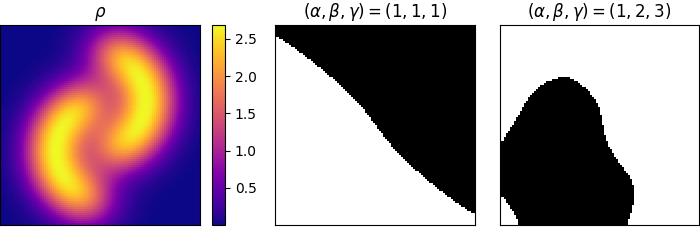
\includegraphics[width=4.5in]{images/moons.png}
}\hspace{0mm}
\subfloat[Noisy concentric circles]{
  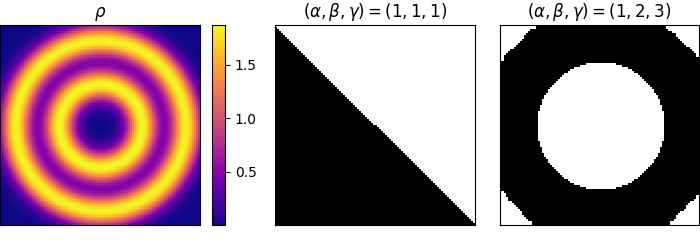
\includegraphics[width=4.5in]{images/circles.png}
}\hspace{0mm}
\subfloat[Long valley]{
  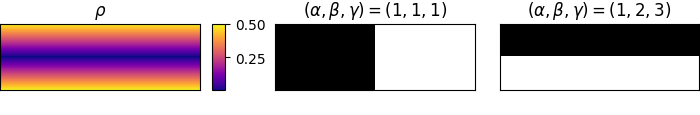
\includegraphics[width=4.5in]{images/trough.png}
}
\caption{
In each row, the first image shows the heat map of a fixed $\rho:\Omega\to\RR_>0$, the second and third images shows the set $\Omega_k$ returned by Algorithm \ref{alg:multiple_cuts} (displayed in black) for the choices $(\alpha,\beta,\gamma)$ of $(1,1,1)$ and $(1,2,3)$ respectively.
 }
\label{fig:alg}
\end{figure}



\unappendix
\end{appendix}



%\end{document}

\chapter{Geometric Spectral Algorithms and Hardness, with Machine
Learning applications}\label{sec:sgt-main}
%\def\isfocs{1} %%% Zhao define this

\newtheorem{notation}[theorem]{Notation}
%\newtheorem{proof}[theorem]{Proof}
\newtheorem{assumption}[theorem]{Assumption}
\newtheorem{proposition}[theorem]{Proposition}
\newtheorem{example}[theorem]{Example}
\newtheorem{open}[theorem]{Open Problem}
\newtheorem{hypothesis}[theorem]{Hypothesis}

\newcommand{\E}{\mathbf{E}}
\newcommand{\T}{\mathcal{T}}
%\newcommand{\poly}{\mathrm{poly}}
%\newcommand{\sign}{\mathrm{sign}}
%\newcommand{\tr}{\mathrm{tr}}
%\newcommand{\polylog}{\mathrm{polylog}}
%\newcommand{\Ceff}{\mathtt{Ceff}}
%\newcommand{\Ham}{\mathrm{Ham}}
%\newcommand{\wh}{\widehat}
%\newcommand{\wt}{\widetilde}
%\newcommand{\ov}{\overline}
%\newcommand{\mc}{\mathcal}
%\renewcommand{\tilde}{\wt}
%\renewcommand{\hat}{\wh}
%\renewcommand{\bar}{\ov}
%\renewcommand{\k}{\mathsf{K}}
%\newcommand{\Reff}{\mathtt{Reff}}
%\newcommand{\true}{\mathtt{true}}
%\newcommand{\false}{\mathtt{false}}
%\newcommand{\KAdjE}{\mathsf{KAdjE}}
%\newcommand{\KLapE}{\mathsf{KLapE}}
%\newcommand{\KDF}{\mathrm{KDF}}
%\newcommand{\KDE}{\mathrm{KDE}}
%\newcommand{\cts}{\mathrm{cts}}
%\newcommand{\dis}{\mathrm{dis}}
%\newcommand{\WSPD}{\mathrm{WSPD}}
%\newcommand{\dist}{\mathrm{dist}}
%\renewcommand{\d}{\mathrm{d}}
%\newcommand{\bdeg}{\mathrm{bdeg}}
%\newcommand{\SETH}{\mathsf{SETH}}
%\newcommand{\ANN}{\mathsf{ANN}}
%\newcommand{\RecoverExpander}{\textsc{RecoverExpander}}
%\newcommand{\SparsifyInner}{\textsc{SparsifyInner}}
%\newcommand{\LowDiamSet}{\textsc{LowDiamSet}}
%\newcommand{\ReffQuery}{\textsc{ReffQuery}}
%\newcommand{\ReffPreproc}{\textsc{ReffPreproc}}
%\newcommand{\UnweightedCover}{\textsc{UnweightedCover}}
%\newcommand{\BoundedCover}{\textsc{BoundedCover}}
%\newcommand{\TwoBoundedCover}{\textsc{TwoBoundedCover}}
%\newcommand{\LogCover}{\textsc{LogCover}}
%\newcommand{\DesiredCover}{\textsc{DesiredCover}}
%\newcommand{\IntervalFamily}{\textsc{IntervalFamily}}
%\newcommand{\OversamplingWithCover}{\textsc{OversamplingWithCover}}

\def\Z{{\mathbb Z}}
\def\N{{\mathbb N}}
\def\R{{\mathbb R}}
\def\Q{{\mathbb Q}}
\def\eps{\varepsilon}
\renewcommand{\epsilon}{\eps}


\definecolor{b2}{RGB}{51,153,255}
\definecolor{mygreen}{RGB}{80,180,0}
 \newcommand{\Zhao}[1]{{\color{mygreen}[Zhao: #1]}}
%\newcommand{\Zhao}[1]{}
\newcommand{\Josh}[1]{{\color{b2}[Josh: #1]}}
\newcommand{\josh}[1]{{\color{b2}[Josh: #1]}}
\newcommand{\Aaron}[1]{{\color{mygreen}[Aaron: #1]}}
% \newcommand{\Aaron}[1]{}
\newcommand{\tim}[1]{{\color{orange}[Tim: #1]}}
\newcommand{\Tim}[1]{{\color{orange}[Tim: #1]}}



%\newcommand{\Zhao}[1]{{\color{mygreen}}}
\renewcommand{\Josh}[1]{{\color{b2}}}
\renewcommand{\josh}[1]{{\color{b2}}}
\renewcommand{\Aaron}[1]{{\color{brown}}}

  \begin{abstract}
For a function $\mathsf{K} : \mathbb{R}^{d} \times \mathbb{R}^{d} \to
\mathbb{R}_{\geq 0}$, and a set $P = \{ x_1, \ldots, x_n\} \subset
\mathbb{R}^d$ of $n$ points, the $\mathsf{K}$ graph $G_P$ of $P$ is the
complete graph on $n$ nodes where the weight between nodes $i$ and $j$
is given by $\mathsf{K}(x_i, x_j)$. In this chapter, we study when efficient spectral graph theory is possible on these graphs. We investigate whether or not it is possible to solve the following problems in $n^{1+o(1)}$ time for a $\mathsf{K}$-graph $G_P$ when $d < n^{o(1)}$:

\begin{itemize}
\item Multiply a given vector by the adjacency matrix or Laplacian matrix of $G_P$
\item Find a spectral sparsifier of $G_P$
\item Solve a Laplacian system in $G_P$'s Laplacian matrix
\end{itemize}
    
For each of these problems, we consider all functions of the form $\mathsf{K}(u,v) = f(\|u-v\|_2^2)$ for a function $f:\mathbb{R} \rightarrow \mathbb{R}$. We provide algorithms and comparable hardness results for many such $\mathsf{K}$, including the Gaussian kernel, Neural tangent kernels, and more. For example, in dimension $d = \Omega(\log n)$, we show that there is a parameter associated with the function $f$ for which low parameter values imply $n^{1+o(1)}$ time algorithms for all three of these problems and high parameter values imply the nonexistence of subquadratic time algorithms assuming Strong Exponential Time Hypothesis ($\mathsf{SETH}$), given natural assumptions on $f$.

As part of our results, we also show that the exponential dependence on the dimension $d$ in the celebrated fast multipole method of Greengard and Rokhlin cannot be improved, assuming $\mathsf{SETH}$, for a broad class of functions $f$. To the best of our knowledge, this is the first formal limitation proven about fast multipole methods. 




  \end{abstract}

%\pagenumbering{roman}

{\hypersetup{linkcolor=black}
\tableofcontents
}

\newpage

% \setcounter{page}{1}
% \pagenumbering{arabic}

 
\section{Introduction}\label{sec:intro}

Linear algebra has a myriad of applications throughout computer science and physics. Consider the following seemingly unrelated tasks:

\vspace{1mm}
\begin{compactenum}
    \item \textbf{$n$-body simulation (one step)}: Given $n$ bodies $X$ located at points in $\mathbb{R}^d$, compute the gravitational force on each body induced by the other bodies.
    \item \textbf{Spectral clustering}: Given $n$ points $X$ in $\mathbb{R}^d$, partition $X$ by building a graph $G$ on the points in $X$, computing the top $k$ eigenvectors of the Laplacian matrix $L_G$ of $G$ for some $k\ge 1$ to embed $X$ into $\mathbb{R}^k$, and run $k$-means on the resulting points.
    \item \textbf{Semi-supervised learning}: Given $n$ points $X$ in $\mathbb{R}^d$ and a function $g:X\rightarrow \mathbb{R}$ whose values on some of $X$ are known, extend $g$ to the rest of $X$.
\end{compactenum}

\vspace{1mm}

Each of these tasks has seen much work throughout numerical analysis, theoretical computer science, and machine learning. The first task is a celebrated application of the fast multipole method of Greengard and Rokhlin~\cite{gr87, gr88, gr89}, voted one of the top ten algorithms of the twentieth century by the editors of \emph{Computing in Science and Engineering}~\cite{dongarra2000guest}.
The second task is \emph{spectral clustering} \cite{njw02, lwdh13}, a popular algorithm for clustering data. The third task is to label a full set of data given only a small set of partial labels~\cite{z05survey, csbz09, zl05}, which has seen increasing use in machine learning. One notable method for performing semi-supervised learning is the graph-based Laplacian regularizer method~\cite{lszlh19,zl05, bns06,z05}.

Popular techniques for each of these problems benefit from primitives in spectral graph theory on a special class of dense graphs called \emph{geometric graphs}. For a function $\k:\mathbb{R}^d\times \mathbb{R}^d\rightarrow \mathbb{R}$ and a set of points $X\subseteq \mathbb{R}^d$, the \emph{$\k$-graph on $X$} is a graph with vertex set $X$ and edges with weight $\k(u,v)$ for each pair $u,v\in X$. Adjacency matrix-vector multiplication, spectral sparsification, and Laplacian system solving in geometric graphs are directly relevant to each of the above problems, respectively:

\vspace{1mm}
\begin{compactenum}
\item \textbf{$n$-body simulation (one step)}: For each $i\in \{1,2,\hdots,d\}$, make a weighted graph $G_i$ on the points in $X$, in which the weight of the edge between the points $u,v\in X$ in $G_i$ is $\k_i(u,v) := (\frac{G_{\text{grav}} \cdot m_u \cdot m_v}{\|u - v\|_2^2})(\frac{v_i - u_i}{\|u - v\|_2})$,  where $G_{\text{grav}}$ is the gravitational constant and $m_x$ is the mass of the point $x\in X$. Let $A_i$ denote the weighted adjacency matrix of $G_i$. Then $A_i\textbf{1}$ is the vector of $i$th coordinates of force vectors. In particular, gravitational force can be computed by doing $O(d)$ adjacency matrix-vector multiplications, where each adjacency matrix is that of the $\k_i$-graph on $X$ for some $i$.

\item \textbf{Spectral clustering}: Make a $\k$ graph $G$ on $X$. In applications, $\k(u,v) = f(\|u-v\|_2^2)$, where $f$ is often chosen to be $f(z) = e^{-z}$~\cite{l07,njw02}. Instead of directly running a spectral clustering algorithm on $L_G$, one popular method is to construct a sparse matrix $M$ approximating $L_G$ and run spectral clustering on $M$ instead~\cite{chl16,csblc11, kmt12}. Standard sparsification methods in the literature are heuristical, and include the widely used Nystrom method which uniformly samples rows and columns from the original matrix~\cite{cjkmm13}. 

If $H$ is a spectral sparsifier of $G$, it has been suggested that spectral clustering with the top $k$ eigenvectors of $L_H$ performs just as well in practice as spectral clustering with the top $k$ eigenvectors of $L_G$~\cite{chl16}. 
One justification is that since $H$ is a spectral sparsifier of $G$, the eigenvalues of $L_H$ are at most a constant factor larger than those of $L_G$, so cuts with similar conductance guarantees are produced. Moreover, spectral clustering using sparse matrices like $L_H$ is known to be faster than spectral clustering on dense matrices like $L_G$ ~\cite{chl16, cjkmm13, kmt12}.

\item \textbf{Semi-supervised learning}: An important subroutine in semi-supervised learning is completion based on $\ell_2$-minimization~\cite{z05, z05survey, lszlh19}. Specifically, given values $g_v$ for $v\in Y$, where $Y$ is a subset of $X$, find the vector $g\in \mathbb{R}^n$ (variable over $X\setminus Y$) that minimizes
$\sum_{u,v\in X,u\ne v} \k(u,v) (g_u - g_v)^2.$
The vector $g$ can be found by solving a Laplacian system on the $\k$-graph for $X$.
\end{compactenum}
\vspace{1mm}

In the first, second, and third tasks above, a small number of calls to matrix-vector multiplication, spectral sparsification, and Laplacian system solving, respectively, were made on geometric graphs. One could solve these problems by first explicitly writing down the graph $G$ and then using near-linear time algorithms \cite{ss11,ckmpprx14} to multiply, sparsify, and solve systems. However, this requires a minimum of $\Omega(n^2)$ time, as $G$ is a dense graph.

In this chapter, we initiate a theoretical study of the geometric graphs for which efficient spectral graph theory is possible. In particular, we attempt to determine for which (a) functions $\k$ and (b) dimensions $d$ there is a much faster, $n^{1+o(1)}$-time algorithm for each of (c) multiplication, sparsification, and Laplacian solving. Before describing our results, we elaborate on the choices of (a), (b), and (c) that we consider in this work.

We start by discussing the functions $\k$ that we consider (part (a)). Our results primarily focus on the class of functions of the form $\k(u,v) = f(\|u-v\|_2^2)$ for a function $f:\mathbb{R}_{\ge 0}\rightarrow \mathbb{R}$ for $u,v\in \mathbb{R}^d$. Study of these functions dates back at least eighty years, to the early work of Bochner, Schoenberg, and John Von Neumann on metric embeddings into Hilbert Spaces~\cite{b33, s37, ns41}. These choices of $\k$ are ubiquitous in applications, like the three described above, since they naturally capture many kernel functions $\k$ from statistics and machine learning, including the Gaussian kernel $(e^{-\|u-v\|_2^2})$, the exponential kernel $(e^{-\|u-v\|_2})$, the power kernel $(\|u-v\|_2^q)$ for both positive and negative $q$, the logarithmic kernel ($\log (\|u-v\|_2^q + c)$), and more~\cite{s10, z05, btb05}.  See Section~\ref{subsec:relatedwork} below for even more popular examples. In computational geometry, many transformations of distance functions are also captured by such functions $\k$, notably in the case when $\k(u,v) = \|u-v\|_2^q$~\cite{l82, as14,acx19, cms20}. 

We would also like to emphasize that many kernel functions which do not at first appear to be of the form $f(\|u-v\|_2^2)$ can be rearranged appropriately to be of this form. For instance, in
\ifdefined\isfocs
the full version
\else
Section~\ref{sec:ntk} below 
\fi
we show that the recently popular Neural Tangent Kernel is of this form, so our results apply to it as well.
That said, to emphasize that our results are very general, we will mention later how they also apply to some functions of the form $\k(u,v) = f(\langle u,v\rangle )$, including $\k(u,v) = |\langle u,v\rangle |$.

Next, we briefly elaborate on the problems that we consider (part (c)). For more details, see 
\ifdefined\isfocs
the full version. 
\else
Section \ref{sec:preli}. 
\fi
The points in $X$ are assumed to be real numbers stated with $\polylog(n)$ bits of precision. Our algorithms and hardness results pertain to algorithms that are allowed some degree of approximation. For an error parameter $\epsilon > 0$, our multiplication and Laplacian system solving algorithms produce solutions with $\epsilon$-additive error, and our sparsification algorithms produce a graph $H$ for which the Laplacian quadratic form $(1 \pm \epsilon)$-approximates that of $G$.

Matrix-vector multiplication, spectral sparsification, and Laplacian system solving are very natural linear algebraic problems in this setting, and have many applications beyond the three we have focused on ($n$-body simulation, spectral clustering, and semi-supervised learning). See Section~\ref{subsec:relatedwork} below where we expand on more applications.

Finally, we discuss dependencies on the dimension $d$ and the accuracy $\epsilon$ for which $n^{1+o(1)}$ algorithms are possible (part (b)). Define $\alpha$, a measure of the `diameter' of the point set and $f$, as
$$\alpha := \frac{ \max_{u,v \in X} f( \| u - v \|_2^2 ) }{ \min_{u,v \in X} f( \| u - v \|_2^2 ) } + \frac{ \max_{u,v \in X}  \| u - v \|_2^2  }{ \min_{u,v \in X}  \| u - v \|_2^2  }.$$
It is helpful to have the following two questions in mind when reading our results:

\vspace{2mm}
\begin{compactitem}
\item (High-dimensional algorithms, e.g. $d = \Theta(\log n)$) Is there an algorithm which runs in time $\poly(d, \log(n\alpha/\epsilon)) n^{1+o(1)}$ for multiplication and Laplacian solving? Is there an algorithm which runs in time $\poly(d, \log(n\alpha))n^{1+o(1)}$ for sparsification when $\epsilon=1/2$?

\item (Low-dimensional algorithms, e.g. $d = o(\log n)$) Is there an algorithm which runs in time $(\log(n\alpha/\epsilon))^{O(d)} n^{1+o(1)}$ for multiplication and Laplacian solving? Is there a sparsification algorithm which runs in time $(\log(n\alpha))^{O(d)} n^{1+o(1)}$ when $\epsilon=1/2$?
\end{compactitem}
\vspace{2mm}

We will see that there are many important functions $\k$ for which there are such efficient low-dimensional algorithms, but no such efficient high-dimensional algorithms. In other words, these functions $\k$ suffer from the classic `curse of dimensionality.' At the same time, other functions $\k$ will allow for efficient low-dimensional and high-dimensional algorithms, while others won't allow for either.

We now state our results. We will give very general classifications of functions $\k$ for which our results hold, but afterwards in Section~\ref{sec:resultstable} we summarize the results for a few particular functions $\k$ of interest. The main goal of our results is as follows:


\textbf{Goal}: For each problem of interest (part (c)) and dimension $d$ (part (b)), find a natural parameter $p_f > 0$ associated with the function $f$ for which the following dichotomy holds:

\begin{compactitem}
    \item If $p_f$ is high, then the problem cannot be solved in subquadratic time assuming $\SETH$ on points in dimension $d$.
    \item If $p_f$ is low, then the problem of interest can be solved in almost-linear time ($n^{1+o(1)}$ time) on points in dimension $d$.
\end{compactitem}



As we will see shortly, the two parameters $p_f$ which will characterize the difficulties of our problems of interest in most settings are the \emph{approximate degree} of $f$, and a parameter related to how \emph{multiplicatively Lipschitz} $f$ is. We define both of these in the next section.



\subsection{High-dimensional results}\label{subsubsec:highdimmult}

We begin in this subsection by stating our results about which functions have $\poly(d,\log(\alpha),\log(1/\epsilon)) \cdot$ $n^{1+o(1)}$-time algorithms for multiplication and Laplacian solving and $\poly(d,\log(\alpha),1/\epsilon)\cdot n^{1+o(1)}$-time algorithms for sparsification. When reading these results, it is helpful to think of $d = \Theta(\log n)$, $\alpha = 2^{\text{polylog}(n)}$, $\epsilon = 1/2^{\polylog(n)}$ for multiplication and Laplacian solving, and $\epsilon = 1/2$ for sparsification. With these parameter settings, $\poly(d)n^{1+o(1)}$ is almost-linear time, while $2^{O(d)}n^{1+o(1)}$ time is not. For results about algorithms with runtimes that are exponential in $d$, see 
\ifdefined\isfocs
the full version.
\else
Section \ref{sec:low-dim-summary}.
\fi

\subsubsection{Multiplication} 

In high dimensions, we give a full classification of when the matrix-vector multiplication problems are easy for kernels of the form $\k(u,v) = f(\|u - v\|_2^2)$ for some function $f:\mathbb{R}_{\ge 0}\rightarrow \mathbb{R}_{\ge 0}$ that is analytic on an interval. We show that the problem can be efficiently solved only when $\k$ is very well-approximated by a simple polynomial kernel. That is, we let $p_f$ denote the minimum degree of a polynomial that $\eps$-additively-approximates the function $f$.

\begin{theorem}
[Informal version of Theorem~\ref{thm:hardnessapprox} and Corollary~\ref{cor:kernelalg}]\label{thm:informal-high}
%\ifdefined\isfocs\else[Informal version of Theorem~\ref{thm:hardnessapprox} and Corollary~\ref{cor:kernelalg}]\fi\label{thm:informal-high} 
For any function $f : \R_+ \to \R_+$ which is analytic on an interval $(0,\delta)$ for any $\delta$ $>0$, and any $0 < \eps < 2^{-\polylog(n)}$, consider the following problem: given as input $x_1, \ldots, x_n \in \R^d$ with $d = \Theta(\log n)$ which define a $\k$ graph $G$ via $\k(x_i, x_j) = f(\|x_i -x_j\|_2^2)$, and a vector $y \in \{0,1\}^n$, compute an $\eps$-additive-approximation to $L_G \cdot y$. 
\begin{compactitem}
    \item If $f$ can be $\eps$-additively-approximated by a polynomial of degree at most $o(\log n)$, then the problem can be solved in $n^{1+o(1)}$ time.
    \item Otherwise, assuming $\SETH$, the problem requires time $n^{2 - o(1)}$.
\end{compactitem}
The same holds for $L_G$, the Laplacian matrix of $G$, replaced by $A_G$, the adjacency matrix of $G$.
\end{theorem}

While Theorem \ref{thm:informal-high} yields a parameter $p_f$ that characterizes hardness of multiplication in high dimensions, it is somewhat cumbersome to use, as it can be challenging to show that a function is far from a polynomial. We also show Theorem \ref{thm:hardnessapprox-easy}, which shows that if $f$ has a single point with large $\Theta(\log n)$-th derivative, then the problem requires time $n^{2-o(1)}$ assuming $\SETH$. The Strong Exponential Time Hypothesis ($\SETH$) is a common assumption in fine-grained complexity regarding the difficulty of solving the Boolean satisfiability problem; see 
\ifdefined\isfocs
the full version
\else
section~\ref{sec:fine_grained}
\fi 
for more details. Theorem~\ref{thm:informal-high} informally says that assuming $\SETH$, the curse of dimensionality is inherent in performing adjacency matrix-vector multiplication. In particular, we directly apply this result to the $n$-body problem discussed at the beginning:

\begin{corollary} \label{cor:nbodyhardness}
Assuming $\SETH$, in dimension $d = \Theta(\log n)$ one step of the $n$-body problem requires time $n^{2 - o(1)}$.
\end{corollary}

The fast multipole method of Greengard and Rokhlin~\cite{gr87, gr89} solves one step of this $n$-body problem in time $(\log(n/\epsilon))^{O(d)} n^{1+o(1)}$. Our Corollary~\ref{cor:nbodyhardness} shows that assuming $\SETH$, such an exponential dependence on $d$ is required and cannot be improved. To the best of our knowledge, this is the first time such a formal limitation on fast multipole methods has been proved. This hardness result also applies to fast multipole methods for other popular kernels, like the Gaussian kernel $\k(u,v) = \exp(-\|u - v\|_2^2)$, as well.





\subsubsection{Sparsification}

We next show that sparsification can be performed in almost-linear time in high dimensions for kernels that are ``multiplicatively Lipschitz'' functions of the $\ell_2$-distance. We say $f:\mathbb{R}_{\ge 0}\rightarrow \mathbb{R}_{\ge 0}$ is $(C,L)$-\emph{multiplicatively Lipschitz} for $C > 1, L > 1$ if for all $x\in \mathbb{R}_{\ge 0}$ and all $\rho\in (1/C,C)$,
$$C^{-L} f(x)\le f(\rho x)\le C^L f(x).$$
Here are some popular functions that are helpful to think about in the context of our results:\\
${}$\hspace{4mm}1. $f(z) = z^L$ for any positive or negative constant $L$. This function is $(C,|L|)$-multiplicatively Lipschitz for any $C > 1$. \\
${}$\hspace{4mm}2. $f(z) = e^{-z}$. This function is not $(C,L)$-multiplicatively Lipschitz for any $L > 1$ and $C > 1$. We call this the \emph{exponential function}.\\
${}$\hspace{4mm}3.  The piecewise function $f(z) = e^{-z}$ for $z\le L$ and $f(z) = e^{-L}$ for $z > L$. This function is $(C,O(L))$-multiplicatively Lipschitz for any $C > 1$. We call this a \emph{piecewise exponential function}. \\
${}$\hspace{4mm}4. The piecewise function $f(z) = 1$ for $z\le k$ and $f(z) = 0$ for $z > k$, where $k\in \mathbb{R}_{\ge 0}$. This function is not $(C,L)$-multiplicatively Lipschitz for any $C > 1$ or $L > 1$. This is a \emph{threshold function}.


We show that multiplicatively Lipschitz functions can be sparsified in $n^{1+o(1)} \poly(d)$ time: 

\begin{theorem}[Informal version of Theorem~\ref{thm:sparsify-lipschitz}]\label{thm:informal-sparsify-lipschitz}
%\ifdefined\isfocs\else[Informal version of Theorem~\ref{thm:sparsify-lipschitz}]\fi\label{thm:informal-sparsify-lipschitz} 
For any function $f$ such that $f$ is $(2, L)$-multiplicatively Lipschitz, building a $(1\pm\epsilon)$-spectral sparsifier of the $\k$-graph on $n$ points in $\mathbb{R}^d$ where $\k(u,v) = f(\|u - v\|_2^2)$, with $O(n \log n / \eps^2)$ edges, can be done in time
\begin{align*}
 O(nd \sqrt{L \log n}) + n \log n \cdot 2^{O(\sqrt{L \log n})} \cdot (\log\alpha)/\eps^2 .
\end{align*}
\end{theorem}
This Theorem applies even when $d = \Omega(\log n)$. When $L$ is constant, the running time simplifies to $O(nd \sqrt{ \log n} + n^{1+o(1)} \log \alpha/ \eps^2)$. This covers the case when $f(x)$ is any rational function with non-negative coefficients, like $f(z) = z^L$ or $f(z) = z^{-L}$. 

It may seem more natural to instead define $L$-multiplicatively Lipschitz functions, without the parameter $C$, as functions with $\rho^{-L} f(x)\le f(\rho x)\le \rho^L f(x)$ 
for all $\rho$ and $x$. Indeed, an $L$-multiplicatively Lipschitz function is also $(C,L)$-multiplicative Lipschitz for any $C>1$, so our results show that efficient sparsification is possible for such functions. However, the parameter $C$ is necessary to characterize when efficient sparsification is possible. Indeed, as in Theorem~\ref{thm:informal-sparsify-lipschitz} above, it is sufficient for $f$ to be $(C,L)$-multiplicative Lipschitz for a $C$ that is bounded away from 1. To complement this result, we also show a lower bound for sparsification for any function $f$ which is not $(C,L)$-multiplicatively Lipschitz for any $L$ and sufficiently large $C$:


\begin{theorem}[Informal version of Theorem \ref{thm:high-spars-hard}]\label{thm:informal-high-spars-hard}
%\ifdefined\isfocs \else[Informal version of Theorem \ref{thm:high-spars-hard}]\fi\label{thm:informal-high-spars-hard}
Consider an $L > 1$. There is some sufficiently large value $C_L > 1$ depending on $L$ such that for any decreasing function $f:\mathbb{R}_{\ge 0}\rightarrow \mathbb{R}_{\ge 0}$ that is not $(C_L,L)$-multiplicatively Lipschitz, no $O(n2^{L^{.48}})$-time algorithm for constructing an $O(1)$-spectral sparsifier of the $\k$-graph of a set of $n$ points in $O(\log n)$ dimensions exists assuming $\SETH$, where $\k(x,y) = f(\|x-y\|_2^2)$.
\end{theorem}

For example, when $L = \Theta(\log^{2+\delta} n)$ for some constant $\delta > 0$, Theorem~\ref{thm:informal-high-spars-hard} shows that there is a $C$ for which, whenever $f$ is not $(C,L)$-multiplicatively Lipschitz, the sparsification problem cannot be solved in time $n^{1+o(1)}$ assuming $\SETH$.

Bounding $C$ in terms of $L$ above is important. For example, if $C$ is small enough that $C^L = 2$, then $f$ could be close to constant. Such $\k$-graphs are easy to sparsify by uniformly sampling edges, so one cannot hope to show hardness for such functions.

Theorem~\ref{thm:informal-high-spars-hard} shows that geometric graphs for threshold functions, the exponential function, and the Gaussian kernel do not have efficient sparsification algorithms. Furthermore, this hardness result essentially completes the story of which \emph{decreasing} functions can be sparsified in high dimensions, modulo a gap of $L^{.48}$ versus $L$ in the exponent. The tractability landscape is likely much more complicated for non-decreasing functions. That said, many of the kernels used in practice, like the Gaussian kernel, are decreasing functions of distance, so our dichotomy applies to them.

We also show that our techniques for sparsification extend beyond kernels that are functions of $\ell_2$ norms; specifically $\k(u,v) = |\langle u,v\rangle|$:

\begin{lemma}[Informal version of Lemma \ref{lem:inner-sparsify}]\label{thm:sparsabsinnerproduct} %\ifdefined\isfocs\else[Informal version of Lemma \ref{lem:inner-sparsify}]\fi \label{thm:sparsabsinnerproduct}
The $\k(u,v) = |\langle u,v\rangle|$-graph on $n$ points in $\mathbb{R}^d$ can be $\epsilon$-approximately sparsified in $n^{1+o(1)} \poly(d) /\epsilon^2$ time.
\end{lemma}

\subsubsection{Laplacian solving}

Laplacian system solving has a similar tractability landscape to that of adjacency matrix multiplication. We prove the following algorithmic result for solving Laplacian systems:

\begin{theorem}[Informal version of Corollary~\ref{cor:exactmonomial} and Proposition~\ref{prop:woodbury}]\label{thm:informal-lapl-poly}
%\ifdefined\isfocs \else[Informal version of Corollary~\ref{cor:exactmonomial} and Proposition~\ref{prop:woodbury}]\fi\label{thm:informal-lapl-poly}
There is an algorithm that takes $ n^{1+o(1)} \poly(d,\log(n\alpha/\epsilon))$ time to $\epsilon$-approximately solve Laplacian systems on $n$-vertex $\k$-graphs, where $\k(u,v) = f(\|u-v\|_2^2)$ for some (nonnegative) polynomial $f$.\footnote{$f$ is a nonnegative function if $f(x) \geq 0$ for all $x \geq 0$.}
\end{theorem}

We show that this theorem is nearly tight via two hardness results. The first applies to multiplicatively Lipschitz kernels, while the second applies to kernels that are not multiplicatively Lipschitz. The second hardness result only works for kernels that are decreasing functions of $\ell_2$ distance. We now state our first hardness result: 

\begin{corollary}\label{cor:introsystemhardhighdim}
Consider a function $f$ that is $(2,o(\log n))$-multiplicatively Lipschitz for which $f$ cannot be $(\epsilon=2^{-\poly(\log  n)})$-approximated by a polynomial of degree at most $o(\log n)$. Then, assuming $\SETH$, there is no $n^{1+o(1)} \poly(d, \log(\alpha n/\epsilon))$-time algorithm for $\epsilon$-approximately solving Laplacian systems in the $\k$-graph on $n$ points, where $\k(u,v) = f(\|u-v\|_2^2)$.
\end{corollary}
\ifdefined\isfocs
In the full version, 
\else
In Section~\ref{sec:equivalence},
\fi
we will see, using an iterative refinement approach, that if a $\k$ graph can be efficiently sparsified, then there is an efficient Laplacian multiplier for $\k$ graphs if and only if there is an efficient Laplacian system solver for $\k$ graphs. Corollary~\ref{cor:introsystemhardhighdim} then follows using this connection: it describes functions which we have shown have efficient sparsifiers but not efficient multipliers.

Corollary~\ref{cor:introsystemhardhighdim}, which is the first of our two hardness results in this setting, applies to slowly-growing functions that do not have low-degree polynomial approximations, like $f(z) = 1/(1 + z)$. Next, we state our second hardness result:

\begin{theorem}[Informal version of Theorem \ref{thm:high-lsolve-hard}]\label{thm:informal-high-lsolve-hard}
%\ifdefined\isfocs \else[Informal version of Theorem \ref{thm:high-lsolve-hard}]\fi\label{thm:informal-high-lsolve-hard}
Consider an $L > 1$. There is some sufficiently large value $C_L > 1$ depending on $L$ such that for any decreasing function $f:\mathbb{R}_{\ge 0}\rightarrow \mathbb{R}_{\ge 0}$ that is not $(C_L,L)$-multiplicatively Lipschitz, no $O(n  2^{L^{.48}} \log \alpha)$-time algorithm exists for solving Laplacian systems $2^{-\poly(\log n)}$ approximately in the $\k$-graph of a set of $n$ points in $O(\log n)$ dimensions assuming $\SETH$, where $\k(u,v) = f(\|u-v\|_2^2)$. 
\end{theorem}

This yields a quadratic time hardness result when $L = \Omega(\log^2 n)$. By comparison, the first hardness result, Corollary~\ref{cor:introsystemhardhighdim}, only applied for $L = o(\log n)$. In particular, this shows that for non-Lipschitz functions like the Gaussian kernel, the problem of solving Laplacian systems and, in particular, doing semi-supervised learning, cannot be done in almost-linear time assuming $\SETH$.





\subsection{Our Techniques}

\subsubsection{Multiplication}

Our goal in matrix-vector multiplication is, given points $P = \{ x_1, \ldots, x_n\} \subset \R^d$ and a vector $y \in \R^n$, to compute a $(1 \pm \eps)$-approximation to the vector $L_G \cdot y$ where $L_G$ is the Laplacian matrix of the $\k$ graph on $P$, for $\eps = n^{-\Omega(1)}$ (see
\ifdefined\isfocs
the full version
\else
Definition~\ref{def:approxmult}\fi for the precise error guarantees on $\eps$). We call this the $\k$ Laplacian Evaluation ($\KLapE$) problem. A related problem, in which the Laplacian matrix $L_G$ is replaced by the adjacency matrix $A_G$, is the $\k$ Adjacency Evaluation ($\KAdjE$) problem.

We begin by showing a simple, generic equivalence between $\KLapE$ and $\KAdjE$ for any $\k$: an algorithm for either one can be used as a black box to design an algorithm for the other with only negligible blowups to the running time and error. It thus suffices to design algorithms and prove lower bounds for $\KAdjE$.

\paragraph*{Algorithmic Techniques}

We use two primary algorithmic tools: the Fast Multipole Method (FMM), and a `kernel method' for approximating $A_G$ by a low-rank matrix.

FMM is an algorithmic technique for computing aggregate interactions between $n$ bodies which has applications in many different areas of science. Indeed, when the interactions between bodies is described by our function $\k$, then the problem solved by FMM coincides with our $\KAdjE$ problem. 

Most past work on FMM either considers the low-dimensional case, in which $d$ is a small constant, or else the low-error case, in which $\eps$ is a constant. Thus, much of the literature does not consider the simultaneous running time dependence of FMM on $\eps$ and $d$. In order to solve $\KAdjE$, we need to consider the high-dimensional, high-error case. We thus give a clean mathematical overview and detailed analysis of the running time of FMM in 
\ifdefined\isfocs
the full version,
\else Section~\ref{sec:fastmm},
\fi
following the seminal work of Greengard and Strain~\cite{gs91}, which may be of independent interest.  

As discussed in section~\ref{subsubsec:highdimmult} above, the running time of FMM depends exponentially on $d$, and so it is most useful in the low-dimensional setting. Our main algorithmic tool in high dimensions is a low-rank approximation technique: we show that when $f(x)$ can be approximated by a sufficiently low-degree polynomial (e.g. any degree $o(\log n)$ suffices in dimension $\Theta(\log n)$), then we can quickly find a low-rank approximation of the adjacency matrix $A_G$, and use this to efficiently multiply by a vector. Although this seems fairly simple, in Theorem~\ref{thm:informal-high} we show it is optimal: when such a low-rank approximation is not possible in high dimensions, then $\SETH$ implies that $n^{2 - o(1)}$ time is required for $\KAdjE$.

The simplest way to show that $f(x)$ can be approximated by a low-degree polynomial is by truncating its Taylor series. In fact, the FMM \emph{also} requires that a truncation of the Taylor series of $f$ gives a good approximation to $f$. By comparison, the FMM puts more lenient restrictions on what degree the series must be truncated to in low dimensions, but in exchange adds other constraints on $f$, including that $f$ must be monotone. \ifdefined\isfocs
See the full version 
\else
See Section~\ref{sec:fastmm_general} and Corollary~\ref{cor:kernelalg} 
\fi 
for more details.


\paragraph*{Lower Bound Techniques}

We now sketch the proof of Theorem~\ref{thm:informal-high}, our lower bound for $\KAdjE$ for many functions $\k$ in high enough dimensions (typically $d = \Omega(\log n)$), assuming $\SETH$. Although $\SETH$ is a hardness hypothesis about the Boolean satisfiability problem, a number of recent results~\cite{aw15,r18,c18,sm19} have showed that it implies hardness for a variety of \emph{nearest neighbor search} problems. Our lower bound approach is hence to show that $\KAdjE$ is useful for solving nearest neighbor search problems.

The high-level idea is as follows. Suppose we are given as input points $X = \{ x_1, \ldots, x_n\} \subset \{0,1\}^d$, and our goal is to find the closest pair of them. For each $\ell \in \{1,2,\ldots,d\}$, let $c_\ell$ denote the number of pairs of distinct points $x_i, x_j \in X$ with distance $\|x_i - x_j\|_2^2 = \ell$. Using an algorithm for $\KAdjE$ for our function $\k(x,y) = f(\| x-y \|_2^2)$, we can estimate
$$1^\top A_G 1 = \sum_{i \neq j} \k(x_i, x_j) = \sum_{\ell=1}^d c_\ell \cdot f(\ell).$$
Similarly, for any nonnegative reals $a,b \geq 0$, we can take an appropriate affine transformation of $X$ so that an algorithm for $\KAdjE$ can estimate
\begin{align}\label{introeq}\sum_{\ell=1}^d c_\ell \cdot f(a\cdot \ell + b).\end{align}

Suppose we pick real values $a_1, \ldots,a_d,b_1,\ldots,b_d \geq 0$ and define the $d \times d$ matrix $M$ by $M[i,\ell] = f(a_i \cdot \ell + b_i)$. By estimating the sum (\ref{introeq}) for each pair $(a_i,b_i)$, we get an estimate of the matrix-vector product $Mc$, where $c \in \mathbb{R}^d$ is the vector of the $c_\ell$ values. We show that if $M$ has a large enough determinant relative to the magnitudes of its entries, then one can recover an estimate of $c$ itself from this, and hence solve the nearest neighbor problem. 

The main tool we need for this approach is a way to pick $a_1, \ldots,a_d,b_1,\ldots,b_d$ for a function $f$ which cannot be approximated by a low degree polynomial so that $M$ has large determinant. We do this by decomposing $\det(M)$ in terms of the derivatives of $f$ using the Cauchy-Binet formula, and then noting that if $f$ cannot be approximated by a polynomial, then many of the contributions in this sum must be large. The specifics of this construction are quite technical; 
\ifdefined\isfocs
see the full version for the details.
\else
see section~\ref{sec:lbhighdim} for the details.
\fi



\paragraph*{Comparison with Previous Lower Bound Techniques}

Prior work (e.g. \cite{cs17}, \cite{bis17}, \cite{bcis18}) has shown $\SETH$-based fine-grained complexity results for matrix-related computations. For instance, \cite{bis17} showed hardness results for exact algorithms for many machine-learning related tasks, like kernel PCA and gradient computation in training neural networks, while \cite{cs17} and \cite{bcis18} showed hardness results for kernel density estimation. In all of this work, the authors are only able to show hardness for a limited set of kernels. For example, \cite{bis17} shows hardness for kernel PCA only for Gaussian kernels. These limitations arise from the technique used. To show hardness, \cite{bis17} exploits the fact that the Gaussian kernel decays rapidly to obtain a gap between the completeness and soundness cases in approximate nearest neighbors, just as we do for functions $f$ like $f(x) = (1/x)^{\Omega(\log n)}$. The hardness results of \cite{cs17} and \cite{bcis18} employ a similar idea.

As discussed in \emph{Lower Bound Techniques}, we circumvent these limitations by showing that applying the multiplication algorithm for one kernel a small number of times and linearly combining the results is enough to solve Hamming closest pair. This idea is enough to give a nearly tight characterization of the analytic kernels for which subquadratic-time multiplication is possible in dimension $d = \Theta(\log n)$. As a result, by combining with reductions similar to those from past work, our lower bound also applies to a variety of similar problems, including kernel PCA, for a much broader set of kernels than previously known; 
\ifdefined\isfocs
see the full version.
\else
see Section~\ref{subsec:kernelPCA} below for the details.
\fi

Our lower bound is also interesting when compared with the Online Matrix-Vector Multiplication (OMV) Conjecture of Henzinger et al.~\cite{henzinger2015unifying}. In the OMV problem, one is given an $n \times n$ matrix $M$ to preprocess, then afterwards one is given a stream $v_1, \ldots, v_n$ of length-$n$ vectors, and for each $v_i$, one must output $M \times v_i$ before being given $v_{i+1}$. The OMV Conjecture posits that one cannot solve this problem in total time $n^{3-\Omega(1)}$ for a general matrix $M$. 
At first glance, our lower bound may seem to have implications for the OMV Conjecture: For some kernels $\k$, our lower bound shows that for an input set of points $P$ and corresponding adjacency matrix $A_G$, and input vector $v_i$, there is no algorithm running in time $n^{2-\Omega(1)}$ for multiplying $A_G \times v_i$, so perhaps multiplying by $n$ vectors cannot be done in time $n^{3-\Omega(1)}$. However, this is not necessarily the case, since the OMV problem allows $O(n^{2.99})$ time for preprocessing $A_G$, which our lower bound does not incorporate. More broadly, the matrices $A_G$ which we study, which have very concise descriptions compared to general matrices, are likely not the best candidates for proving the OMV Conjecture. That said, perhaps our results can lead to a form of the OMV Conjecture for geometric graphs with concise descriptions.

\subsubsection{Sparsification}

\paragraph*{Algorithmic techniques}

Our algorithm for constructing high-dimensional sparsifiers for $\k(x,y) = f(\|x-y\|_2^2)$, when $f$ is a $(2, L)$ multiplicatively Lipschitz function, involves using three classic ideas: the Johnson Lindenstrauss lemma of random projection~\cite{jl84, im98}, the notion of well-separated pair decomposition from Callahan and Kosaraju~\cite{ck93, ck95}, and spectral sparsification via oversampling~\cite{ss11, kmp10}. Combining these techniques carefully gives us the bounds in Theorem~\ref{thm:informal-sparsify-lipschitz}.

To overcome the `curse of dimensionality', we use the Lindenstrauss lemma to project onto $\sqrt{L \log n}$ dimensions. This preserves all pairs distance, with a distortion of at most $2^{O(\sqrt{\log n/L})}$. Then, using a $1/2$-well-separated pair decomposition partitions the set of projected distances into bicliques, such that each biclique has edges that are no more than $2^{O(\sqrt{\log n/L})}$ larger than the smallest edge in the biclique. This ratio will upper bound the maximum leverage score of an edge in this biclique in the original $\k$-graph. 
Each biclique in the set of projected distances has a one-to-one correspondence to a biclique in the original $\k$-graph. Thus to sparsify our $\k$-graph, we sparsify each biclique in the $\k$-graph by uniform sampling, and take the union of the resulting sparsified bicliques. Due to the $(2, L)$-Lipschitz nature of our function, it is guaranteed that the longest edge in any biclique (measured using $\k(x,y)$) is at most $2^{O(\sqrt{L \log n})}$. This upper bounds the maximum leverage score of an edge in this biclique with respect to the $\k$-graph, which then can be used to upper bound the number of edges we need to sample from each biclique via uniform sampling.
We take the union of these sampled edges over all bicliques, which gives our results for high-dimensional sparsification summarized in Theorem~\ref{thm:informal-sparsify-lipschitz}.
\ifdefined\isfocs
Details can be found in the full version. 
\else
Details can be found in the proof of Theorem~\ref{thm:sparsify-lipschitz} in Section~\ref{sec:sparsify-lipschitz}.
\fi
When $L$ is constant, we get almost linear time sparsification algorithms.

For low dimensional sparsification, we skip the Johnson Lindenstrauss step, and use a $(1+1/L)$-well separated pair decomposition. This gives us a nearly linear time algorithm for sparsifying $(C, L)$ multiplicative Lipschitz functions, when $(2L)^{O(d)}$ is small, which covers the case when $d$ is constant and $L=n^{o(1)}$. 
\ifdefined\isfocs 
See the full version for details.
\else 
See Theorem~\ref{thm:low-sparsify-lipschitz} for details.
\fi

For $\k(u,v) = |\langle u,v\rangle|$, our sparsification algorithm is quite different from the multiplicative Lipschitz setting. In particular, the fact that $\k(u,v) = 0$ on a large family of pairs $u,v\in \mathbb{R}^d$ presents challenges. Luckily, though, this kernel does have some nice structure. For simplicity, just consider defining the $\k$-graph on a set of unit vectors. The weight of any edge in this graph is at most 1 by Cauchy-Schwarz. The key structural property of this graph is that for every set $S$ with $|S| > d+1$, there is a pair $u,v\in S$ for which the $u$-$v$ edge has weight at least $\Omega(1/d)$. In other words, the unweighted graph consisting of edges with weight between $\Omega(1/d)$ and 1 does not have independent sets with size greater than $d+1$. It turns out that all such graphs are dense  \ifdefined\isfocs(see the full version)\else(see Proposition \ref{prop:k-dep-dense})\fi and that all dense graphs have an expander subgraph consisting of a large fraction of the vertices \ifdefined\isfocs(see the full version)\else(see Proposition \ref{prop:dense-has-expander})\fi. Thus, if this expander could be found in $O(n)$ time, we could partition the graph into expander clusters, sparsify the expanders via uniform sampling, and sparsify the edges between expanders via uniform sampling. It is unclear to us how to identify this expander efficiently, so we instead identify clusters with effective resistance diameter $O(\poly(d\log n)/n)$. This can be done via uniform sampling and Johnson-Lindenstrauss \cite{ss11}. As part of the proof, we prove a novel Markov-style lower bound on the probability that effective resistances deviate too low in a randomly sampled graph, which may be of independent interest  
\ifdefined\isfocs
(see the full version).
\else(see Lemma \ref{lem:sparse-lower-tail}).
\fi

\paragraph*{Lower bound techniques}

To prove lower bounds on sparsification for decreasing functions that are not $(C_L,L)$-multiplicatively Lipschitz, we reduce from exact bichromatic nearest neighbors on two sets of points $A$ and $B$. In high dimensions, nearest neighbors is hard even for Hamming distance \cite{r18}, so we may assume that $A,B\subseteq \{0,1\}^d$. In low dimensions, we may assume that the coordinates of points in $A$ and $B$ consist of integers on at most $O(\log n)$ bits. In both cases, the set of possible distances between points in $A$ and $B$ is discrete. We take advantage of the discrete nature of these distance sets to prove a lower bound. In particular, $C_L$ is set so that $C_L$ is the smallest ratio between any two possible distances between points in $A$ and $B$. To see this in more detail, see 
\ifdefined\isfocs
the full version.
\else
Lemma \ref{lem:spars-reduc}.
\fi

Let $x_f$ be a point at which the function $f$ is not $(C_L,L)$-multiplicatively Lipschitz and suppose that we want to solve the decision problem of determining whether or not $\min_{a\in A, b\in B} \|a - b\|_2\le k$. We can do this using sparsification by scaling the points in $A$ and $B$ by a factor of $k/x_f$, sparsifying the $\k$-graph on the resulting points, and thresholding based on the total weight of the resulting $A$-$B$ cut. If there is a pair with distance at most $k$, there is an edge crossing the cut with weight at least $f(x_f)$ because $f$ is a decreasing function. Therefore, the sparsifier has total weight at least $f(x_f)/(1+\epsilon) = f(x_f)/2$ crossing the $A$-$B$ cut by the cut sparsification approximation guarantee. If there is not a pair with distance at most $k$, no edges crossing the cut with weight larger than $f(C_L x_f)\le C_L^{-L} f(x_f)\le ( 1/n^{10} ) \cdot f(x_f)$ by choice of $C_L$. Therefore, the total weight of the $A$-$B$ cut is at most $(1/n^8 ) \cdot f(x_f)$, which means that it is at most $( (1 + \epsilon)/n^8 ) \cdot f(x_f) < f(x_f)/4$ in the sparsifier. In particular, thresholding correctly solves the decision problem and one sparsification is enough to solve bichromatic nearest neighbors.




\subsection{Brief summary of our results in terms of \texorpdfstring{$p_f$}{}}

Before proceeding to the body of the chapter, we summarize our results.
Recall that we consider three linear-algebraic problems in this chapter, along with two different dimension settings (low and high). This gives six different settings to consider. We now define $p_f$ in each of these settings. In all high-dimensional settings, we have found a definition of $p_f$ that characterizes the complexity of the problem. In some low-dimensional settings, we do not know of a suitable definition for $p_f$ and leave this as an open problem. For simplicity, we focus here only on decreasing functions $f$, although all of our algorithms, and most of our hardness results,  hold for more general functions as well.

\begin{table*}[!ht]
\centering
\begin{tabular}{|l|l|l|l|}
    \hline
    {\bf Dimension} & {\bf Multiplication} & {\bf Sparsification} & {\bf Solving} \\ \hline
     $d = \poly(\log n)$ & $f_1$ & $f_1,f_2$ & $f_1$\\ \hline
     $c^{\log^* n} < d < O(\log^{1-\delta} n)$ for  $\delta > 0$ & $f_1,f_2,f_3$ & $f_1,f_2,f_3$ & $f_1,f_2,f_3$ \\ \hline
\end{tabular}\caption{Functions among $f_1,f_2,f_3,f_4$ that have almost-linear time algorithms}\label{tab:examples}
\end{table*}


\begin{compactenum}
    \item Adjacency matrix-vector multiplication
    \begin{enumerate}
        \item High dimensions: $p_f$ is the minimum degree of any polynomial that $1/2^{\text{poly}(\log n)}$-additively approximates $f$. $p_f > \Omega(\log n)$ implies subquadratic-time hardness (Theorem \ref{thm:informal-high} part 2), while $p_f < o(\log n)$ implies an almost-linear time algorithm (Theorem \ref{thm:informal-high}, part 1).
        \item Low dimensions: Not completely understood. The fast multipole method yields an almost-linear time algorithm for some functions, like the Gaussian kernel \ifdefined\isfocs(see the full version)\else(Theorem \ref{thm:fast_gaussian_transform_intro})\fi, but functions exist that are hard in low dimensions \ifdefined\isfocs(see the full version).
        \else(Proposition \ref{prop:low-mult-hard}).\fi
    \end{enumerate}
    \item Sparsification. In both settings, $p_f$ is the minimum value for which $f$ is $(C, p_f)$-multiplicatively Lipschitz, where $C = 1 + 1/p_f^c$ for some constant $c > 0$ independent of $f$.
    \begin{enumerate}
        \item High dimensions: If $p_f > \Omega(\log^2 n)$ and $f$ is nonincreasing, then no subquadratic time algorithm exists (Theorem \ref{thm:informal-high-spars-hard}). If $p_f < o(\log n)$, then an almost-linear time algorithm for sparsification exists (Theorem \ref{thm:informal-sparsify-lipschitz}).
        \item Low dimensions: There is some constant $t > 1$ such that if $p_f > \Omega(n^t)$ and $f$ is nonincreasing, then no subquadratic time algorithm exists \ifdefined\isfocs(see the full version). \else(Theorem \ref{thm:informal-low-spars-hard}).\fi If $p_f < n^{o(1/d)}$, then there is a subquadratic time algorithm \ifdefined\isfocs(see the full version)\else(Theorem \ref{thm:informal-low-sparsify-lipschitz})\fi.
    \end{enumerate}
    \item Laplacian solving.
    \begin{enumerate}
        \item High dimensions: $p_f$ is the maximum of the $p_f$ values in the \emph{Adjacency matrix-vector multiplication} and \emph{Sparsification} settings, with hardness occurring for decreasing functions $f$ if $p_f > \Omega(\log^2 n)$ (Corollary \ref{cor:introsystemhardhighdim} combined with Theorem \ref{thm:informal-high-lsolve-hard}) and an algorithm existing when $p_f < o(\log n)$ (Theorem \ref{thm:informal-lapl-poly}).
        \item Low dimensions: Not completely understood, as in the low-dimensional multiplication setting. As in the sparsification setting, we are able to show that there is a constant $t$ such that if $f$ is nonincreasing and $p_f > \Omega(n^t)$ where $p_f$ is defined as in the \emph{Sparsifiction} setting, then no subquadratic time algorithm exists \ifdefined\isfocs(see the full version).
        \else
        (Theorem \ref{thm:low-lsolve-hard}).
        \fi
    \end{enumerate}
\end{compactenum}

Many of our results are not tight for two reasons: (a) some of the hardness results only apply to decreasing functions, and (b) there are gaps in $p_f$ values between the upper and lower bounds. However, neither of these concerns are important in most applications, as (a) weight often decreases as a function of distance and (b) $p_f$ values for natural functions are often either very low or very high. For example, $p_f > \Omega(\text{polylog}(n))$ for all problems for the Gaussian kernel ($f(x) = e^{-x}$), while $p_f = O(1)$ for sparsification and $p_f > \Omega(\text{polylog}(n))$ for multiplication for the gravitational potential ($f(x) = 1/x$). Resolving the gap may also be difficult, as for intermediate values of $p_f$, the true best running time is likely an intermediate running time of $n^{1 + c + o(1)}$ for some constant $0<c<1$. Nailing down and proving such a lower bound seems beyond the current techniques in fine-grained complexity.

\subsection{Summary of our Results on Examples} \label{sec:resultstable}

To understand our results better, we illustrate how they apply to some examples. For each of the functions $f_i$ given below, make the $\k$-graph, where $\k_i(u,v) = f_i(\|u-v\|_2^2)$:

\begin{compactenum}
\item $f_1(z) = z^k$ for a positive integer constant $k$.
\item $f_2(z) = z^c$ for a negative constant or a positive non-integer constant $c$.
\item $f_3(z) = e^{-z}$ (the Gaussian kernel).
\item $f_4(z) = 1$ if $z\le \theta$ and $f_4(z) = 0$ if $z > \theta$ for some parameter $\theta > 0$ (the threshold kernel).
%\item $f_5(z) = \frac{1}{\pi} (\pi - \cos^{-1}(1-0.5 z) ) \cdot (1-0.5 z) $ (corresponds to the neural tangent kernel \cite{jgh18}; see Section~\ref{sec:ntk})
\end{compactenum}



\josh{We need to put $f_5$ in the appropriate places in the table}

In Table \ref{tab:examples}, we summarize for which of the above functions there are efficient algorithms and for which we have hardness results. There are six regimes, corresponding to three problems (multiplication, sparsification, and solving) and two dimension regimes ($d = \poly(\log n)$ and $d = c^{\log^* n}$). A function is placed in a table cell if an almost-linear time algorithm exists, where runtimes are $n^{1+o(1)}(\log(\alpha n/\epsilon))^t$ in the case of multiplication and system solving and $n^{1+o(1)}(\log(\alpha n))^t/\epsilon^2$ in the case of sparsification for some $t\le O(\log^{1-\delta} n)$ for some $\delta > 0$. Moreover, for each of these functions $f_1, f_2, f_3,$ and $f_4$, if it does not appear in a table cell, then we show a lower bound that no subquadratic time algorithm exists in that regime assuming $\SETH$.



\josh{Note: we don't care if the stuff below is on page 11 or later}

\subsection{Other Related Work} \label{subsec:relatedwork}

\paragraph*{Linear Program Solvers}

Linear Program is a fundamental problem in convex optimization. There is a long list of work focused on designing fast algorithms for linear program \cite{d47,k80,k84,v87,v89_lp,ls14,ls15,cls19,lsz19,song19,b20,blss20,sy20,jswz20}. For the dense input matrix, the state-of-the-art algorithm \cite{jswz20} takes $n^{\max\{\omega,2+1/18\}} \log (1/\eps)$ time, $\omega$ is the exponent of matrix multiplication \cite{aw21}. The solver can run faster when matrix $A$ has some structures, e.g. Laplacian matrix. 

\paragraph*{Laplacian System Solvers}
It is well understood that a Laplacian linear system can be solved in time $\tilde{O} (m \log ( 1 / \eps ) )$, where $m$ is the number of edges in the graph generating the Laplacian~\cite{st04,kmp10,kmp11,kosz13,ls13,ckmpprx14,klpss16,ks16}. This algorithm is very efficient when the graph is sparse. However, in our setting where the $\k$ graph is dense but succinctly describable by only $n$ points in $\R^d$, we aim for much faster algorithms. 

\paragraph*{Algorithms for Kernel Density Function Approximation} A recent line of work by Charikar et al.~\cite{cs17,bcis18} also studies the algorithmic KDE problem. They show, among other things, that kernel density functions for ``smooth'' kernels $\k$ can be estimated in time which depends only polynomially on the dimension $d$, but which depends polynomially on the error $\eps$. We are unfortunately unable to use their algorithms in our setting, where we need to solve $\KAdjE$ with $\eps = n^{-\Omega(1)}$, and the algorithms of Charikar et al. do not run in subquadratic time. We instead design and make use of algorithms whose running times have only polylogarithmic dependences on $\eps$, but often have exponential dependences on $d$.


\paragraph{Kernel Functions}
Kernel functions are useful functions in data analysis, with applications in physics, machine learning, and computational biology~\cite{s10}. There are many kernels studied and applied in the literature; we list here most of the popular examples.

The following kernels are of the form $\k(x,y) = f(\|x-y\|_2^2)$, which
we study in this chapter: the Gaussian kernel \cite{njw02,rr08}, exponential kernel, Laplace kernel \cite{rr08}, rational quadratic kernel, multiquadric kernel \cite{bg97}, inverse multiquadric kernel \cite{m84,m12}, circular kernel \cite{btfb05}, spherical kernel, power kernel \cite{fs03}, log kernel \cite{bg97,m12}, Cauchy kernel \cite{rr08}, and generalized T-Student kernel \cite{btf04}.

For these next kernels, it is straightforward that their corresponding graphs have low-rank adjacency matrices, and so efficient linear algebra is possible using the Woodbury Identity \ifdefined\isfocs(see the full version)\else(see Section~\ref{sec:woodbury_identity} below)\fi: the linear kernel \cite{ssa98,mssmsr99,h07,s14} and the polynomial kernel \cite{cv95,ge08,bossr08,chcrl10}.

Finally, the following relatively popular kernels are not of the form we
directly study in this chapter, and we leave extending our results to them as an important open problem: the Hyperbolic tangent (Sigmoid) kernel \cite{hs97,btb05,jkl09,ksh12,zsjbd17,zsd17,ssbcv17,zsjd19}, spline kernel \cite{g98,u99}, B-spline kernel \cite{h04,m10}, Chi-Square kernel \cite{vz12}, and the histogram intersection kernel and generalized histogram intersection \cite{btb05a}. More interestingly, our result also can be applied to Neural Tangent Kernel \cite{jgh18}, which plays a crucial role in the recent work about convergence of neural network training \cite{ll18,dzps19,als18,als19,sy19,bpsw20,lsswy20,jmsz20}. For more details, we refer the readers to
\ifdefined\isfocs
the full version.
\else
Section~\ref{sec:ntk}.
\fi

\paragraph{Acknowledgements}

The authors would like to thank Lijie Chen for helpful suggestions in the hardness section and explanation of his papers. The authors would like to thank Sanjeev Arora, Simon Du, and Jason Lee for useful discussions about the neural tangent kernel.

 %%% Section 1

%\newpage

\section{Summary of Low Dimensional Results}\label{sec:low-dim-summary}

In the results we've discussed so far, we show that in high-dimensional settings, the curse of dimensionality applies to a wide variety of functions that are relevant in applications, including the Gaussian kernel and inverse polynomial kernels. Luckily, in many settings, the points supplied as input are very low-dimensional. In the classic $n$-body problem, for example, the input points are 3-dimensional. In this subsection, we discuss our results pertaining to whether algorithms with runtimes exponential in $d$ exist; such algorithms can still be efficient in low dimensions $d = o(\log n)$.

\subsection{Multiplication}

The prior work on the fast multipole method ~\cite{gr87, gr88, gr89} yields algorithms with runtime $(\log(n/\epsilon))^{O(d)} n^{1+o(1)}$ for $\epsilon$-approximate adjacency matrix-vector multiplication for a number of functions $\k$, including when $\k(u,v) = \frac{1}{\|u - v\|_2^c}$ for a constant $c$ and when $\k(u,v) = e^{-\|u-v\|_2^2}$. In order to explain what functions $\k$ the fast multipole methods work well for, and to clarify dependencies on $d$ in the literature, we give a complete exposition of how the fast multipole method of~\cite{gs91} works on the Gaussian kernel:

\begin{theorem}[fast Gaussian transform~\cite{gs91}, exposition in Section~\ref{sec:fastmm}]\label{thm:fast_gaussian_transform_intro}
Let $\k(x,y) = \exp (- \| x - y \|_2^2)$. Given a set of points $P \subset \R^d$ with $|P|= n$. Let $G$ denote the $\k$-graph. For any vector $u \in \R^d$, for accuracy parameter $\epsilon$, 
there is an algorithm that runs in 
$
n \log^{O(d)} ( \| u \|_1 / \epsilon ) 
$
time to approximate $A_G \cdot u$ within $\epsilon$ additive error.
\end{theorem}

The fast multipole method is fairly general, and so similar algorithms also exist for a number of other functions $\k$; see Section~\ref{sec:fastmm_general} for further discussion. 
Unlike in the high-dimensional case, we do not have a characterization of the functions for which almost-linear time algorithms exist in near-constant dimension. We leave this as an open problem. Nonetheless, we are able to show lower bounds, even in barely super-constant dimension $d = \exp(\log^*(n))$\footnote{Here, $\log^*(n)$ denotes the \emph{very} slowly growing iterated logarithm of $n$.}, on adjacency matrix-vector multiplication for kernels that are not multiplicatively Lipschitz:

\begin{theorem}[Informal version of Proposition \ref{prop:low-mult-hard}]
For some constant $c>1$, any function $f$ that is not $(C,L)$-multiplicatively Lipschitz for any constants $C > 1, L > 1$  does not have an $n^{1+o(1)}$ time adjacency matrix-vector multiplication (up to $2^{-\poly(\log n)}$ additive error) algorithm in $c^{\log^* n}$ dimensions assuming $\SETH$ when $\k(u,v) = f(\| u - v \|_2^2)$.
\end{theorem}

This includes threshold functions, but does not include piecewise exponential functions. Piecewise exponential functions do have efficient adjacency multiplication algorithms by Theorem \ref{thm:fast_gaussian_transform}.

To illustrate the complexity of the adjacency matrix-vector multiplication problem in low dimensions, we are also able to show hardness for the function $\k(u,v) = |\langle u,v\rangle|$ in nearly constant dimensions. By comparison, we are able to sparsify for this function $\k$, even in very high $d = n^{o(1)}$ dimensions (in Theorem~\ref{thm:sparsabsinnerproduct} above).
\begin{theorem}[Informal version of Corollary \ref{cor:lowdimmultabsinnerproduct}] \label{thm:introlowdimmultabsinnerproduct}
For some constant $c>1$, assuming $\SETH$, adjacency matrix-vector multiplication (up to $2^{-\poly(\log n)}$ additive error) in $c^{\log^* n}$ dimensions cannot be done in subquadratic time in dimension $d = \exp(\log^*(n))$ when $\k(u,v) = |\langle u,v\rangle|$.
\end{theorem}


\subsection{Sparsification}

We are able to give a characterization of the decreasing functions for which sparsification is possible in near-constant dimension. We show that a polynomial dependence on the multiplicative Lipschitz constant is allowed, unlike in the high-dimensional setting:
\begin{theorem}[Informal version of Theorem \ref{thm:low-sparsify-lipschitz}]\label{thm:informal-low-sparsify-lipschitz}
Let $f$ be a $(1 + 1/L,L)$-multiplicatively Lipschitz function and let $\k(u,v) = f(\|u-v\|_2^2)$. Then an $(1\pm\epsilon)$-spectral sparsifier for the $\k$-graph on $n$ points can be found in $ n^{1+o(1)} L^{O(d)} (\log \alpha) /\epsilon^2$ time. 
\end{theorem}

Thus, geometric graphs for piecewise exponential functions with $L = n^{o(1)}$ can be sparsified in almost-linear time when $d$ is constant, unlike in the case when $d = \Omega(\log n)$. In particular, spectral clustering can be done in $O(kn^{1+o(1)})$ time for $k$ clusters in low dimensions. Unfortunately, not all geometric graphs can be sparsified, even in nearly constant dimensions:

\begin{theorem}[Informal version of Theorem \ref{thm:low-spars-hard}]\label{thm:informal-low-spars-hard}
There are constants $c'\in (0,1),c > 1$ and a value $C_L$ given $L > 1$ for which any decreasing function $f$ that is not $(C_L,L)$-multiplicatively Lipschitz does not have an $O(n L^{c'})$ time sparsification algorithm for $\k$-graphs on $c^{\log^*n}$ dimensional points, where $\k(u,v) = f(\|u-v\|_2^2)$.
\end{theorem}

This theorem shows, in particular, that geometric graphs of threshold functions are not sparsifiable in subquadratic time even for low-dimensional pointsets. These two theorems together nearly classify the decreasing functions for which efficient sparsification is possible, up to the exponent on $L$.

\subsection{Laplacian solving}

As in the case of multiplication, we are unable to characterize the functions for which solving Laplacian systems can be done in almost-linear time in low dimensions. That said, we still have results for many functions $\k$, including most kernel functions of interest in applications. We prove most of these using the aforementioned connection from Section~\ref{sec:equivalence}: if a $\k$ graph can be efficiently sparsified, then there is an efficient Laplacian multiplier for $\k$ graphs if and only if there is an efficient Laplacian system solver for $\k$ graphs.

For the kernels $\k(u,v) = 1/\|u-v\|_2^c$ for constants $c$ and the piecewise exponential kernel, we have almost-linear time algorithms in low dimensions by Theorems \ref{thm:sparsify-lipschitz} and \ref{thm:low-sparsify-lipschitz} respectively. Furthermore, the fast multipole method yields almost-linear time algorithms for multiplication. Therefore, there are almost-linear time algorithm for solving Laplacian systems in geometric graphs for these kernels.

A similar approach also yields hardness results. Theorem~\ref{thm:sparsabsinnerproduct} above implies that an almost-linear time algorithm for solving Laplacian systems on $\k$-graphs for $\k(u,v) = |\langle u,v\rangle |$ yields an almost-linear time algorithm for $\k$-adjacency multiplication. However, no such algorithm exists assuming $\SETH$ by Theorem~\ref{thm:introlowdimmultabsinnerproduct} above. Therefore, $\SETH$ implies that no almost-linear time algorithm for solving Laplacian systems in this kernel can exist.

We directly (i.e. without using a sparsifier algorithm) show an additional hardness result for solving Laplacian systems for kernels that are not multiplicatively Lipschitz, like threshold functions of $\ell_2$-distance:

\begin{theorem}[Informal version of Theorem \ref{thm:low-lsolve-hard}]
Consider an $L > 1$. There is some sufficiently large value $C_L > 1$ depending on $L$ such that for any decreasing function $f:\mathbb{R}_{\ge 0}\rightarrow \mathbb{R}_{\ge 0}$ that is not $(C_L,L)$-multiplicatively Lipschitz, no $O(n L^{c'} \log \alpha)$-time algorithm exists for solving Laplacian systems $2^{-\poly(\log n)}$ approximately in the $\k$-graph of a set of $n$ points in $c^{\log^* n}$ dimensions for some constants $c > 1, c'\in (0,1)$ assuming $\SETH$, where $\k(u,v) = f(\|u-v\|_2^2)$.
\end{theorem}
 %%% Section 2 Summary of Low Dimension Results
\section{Preliminaries}\label{sec:preli}

Our results build off of algorithms and hardness results from many different areas of theoretical computer science. We begin by defining the relevant notation and describing the important past work.

\subsection{Notation}

For an $n\in \mathbb{N}_{+}$, let $[n]$ denote the set $\{1,2,\cdots,n\}$.

For any function $f$, we write $\wt{O}(f)$ to denote $f\cdot \log^{O(1)}(f)$. In addition to $O(\cdot)$ notation, for two functions $f,g$, we use the shorthand $f\lesssim g$ (resp. $\gtrsim$) to indicate that $f\leq C g$ (resp. $\geq$) for an absolute constant $C$. We use $f\eqsim g$ to mean $cf\leq g\leq Cf$ for constants $c,C$.

For a matrix $A$, we use $\|A\|_2$ to denote the spectral norm of $A$. Let $A^\top$ denote the transpose of $A$. Let $A^\dagger$ denote the Moore-Penrose pseudoinverse of $A$. Let $A^{-1}$ denote the inverse of a full rank square matrix. 

We say matrix $A$ is positive semi-definite (PSD) if $A = A^\top$ and $x^\top A x \geq 0$ for all $x \in \R^n$. We use $\preceq$, $\succeq$ to denote the semidefinite ordering, e.g. $A \succeq 0$ denotes that $A$ is PSD, and $A \succeq B $ means $A- B \succeq 0$. We say matrix $A$ is positive definite (PD) if $A = A^\top$ and $x^\top A x > 0$ for all $x \in \R^n -\{0\}$. $A \succ B$ means $A-B$ is PD.

For a vector $v$, we denote $\| v \|_p$ as the standard $\ell_p$ norm. For a vector $v$ and PSD matrix $A$, we let $\| v \|_A = (v^\top A v)^{1/2}$.

The iterated logarithm $\log^* : \R \to \Z$ is given by \begin{align*}
    \log^*(n) = \begin{cases}
    0, &\text{ if } n \leq 1 ; \\
    1 + \log^*(\log n), &\text{ otherwise.}
    \end{cases}
\end{align*}

We use $G_{\text{grav}}$ to denote the Gravitational constant.

We define $\alpha$ slightly differently in different sections. Note that both are less than the value of $\alpha$ used in Theorem \ref{thm:informal-sparsify-lipschitz}: 
\begin{table}[!h]\caption{}
\centering
\begin{tabular}{|l|l|l|}
    \hline
    Notation & Meaning & Location \\ \hline
    $\alpha$ & $\frac{ \max_{i,j} f(\| x_i - x_j \|_2^2) }{ \min_{i,j} f( \| x_i - x_j \|_2^2 ) }$  & Section~\ref{sec:equivalence}  \\ \hline
    $\alpha$ & $\frac{\max_{i,j} \| x_i - x_j \|_2 }{\min_{i,j} \| x_i - x_j \|_2}$ & Section~\ref{sec:sparsify-lipschitz} \\ \hline %%% This is Tim section and actually kappa
\end{tabular}
\end{table}


\subsection{Graph and Laplacian Notation}\label{sec:graph_Laplacian_notation}

Let $G = (V,E,w)$ be a connected weighted undirected graph with $n$ vertices and $m$ edges and edge weights $w_e > 0$. We say $r_e = 1/w_e$ is the resistance of edge $e$.
If we give a direction to the edges of $G$ arbitrarily, we can write its Laplacian as $L_G = B^\top W B$, where $W \in \R^{m \times m}$ is the diagonal matrix $W(e,e) = w_e$ and $B \in \R^{m \times n}$ is the signed edge-vertex incidence matrix and can be defined in the following way
\begin{align}\label{eq:def_Laplacian_B}
B(e,v) = \begin{cases}
1,  & \text{~if~$v$~is~$e$'s~head}; \\
-1, & \text{~if~$v$~is~$e$'s~tail};\\
0,  & \text{~otherwise.}
\end{cases}
\end{align}

A useful notion related to Laplacian matrices is the effective resistance of a pair of nodes:
\begin{definition}[Effective resistance]\label{def:effective_resistance}
The effective resistance of a pair of vertices $u,v \in V_G$ is defined as 
\begin{align*}
\Reff_G(u,v) = b_{u,v}^\top L^\dagger b_{u,v}
\end{align*}
where $b_{u,v} \in \R^{|V_G|}$ is an all zero vector except for entries of $1$ at $u$ and $-1$ at $v$.
\end{definition}

Using effective resistance, we can define leverage score
\begin{definition}[Leverage score]\label{def:leverage_score}
The leverage score of an edge $e = (u,v) \in E_G$ is defined as 
\begin{align*}
l_e = w_e \cdot \Reff_G(u,v).
\end{align*}
\end{definition}

We define a useful notation called electrical flow
\begin{definition}[Electrical flow]\label{def:electrical_flow}
Let $B \in \R^{m \times n}$ be defined as Eq.~\eqref{eq:def_Laplacian_B}, for a given demand vector $d \in \R^n$, we define electrical flow $f \in \R^m$ as follows:
\begin{align*}
f = \arg\min_{ f : B^\top f = d } \sum_{ e \in E_G } f_e^2 /w_e .
\end{align*}
\end{definition}

We let $d(i)$ denote the degree of vertex $i$. For any set $S \subseteq V$, we define volume of $S$: $\mu(S) = \sum_{i \in S} d(i)$. It is obvious that $\mu(V) = 2|E|$. For any two sets $S, T \subseteq V$, let $E(S,T)$ be the set of edges connecting a vertex in $S$ with a vertex in $T$. We call $\Phi(S)$ to be the conductance of a set of vertices $S$, and can be formally defined as
\begin{align*}
\Phi(S) = \frac{ | E(S, V \setminus S) | }{ \min ( \mu (S) , \mu ( V \setminus S ) ) }.
\end{align*}
We define the notation conductance, which is standard in the literature of graph partitioning and graph clustering \cite{st04,kvv04,acl06,ap09,lrtv11,zlm13,lz14}.
\begin{definition}[Conductance]\label{def:conductance}
The conductance of a graph $G$ is defined as follows:
\begin{align*}
\Phi_G = \min_{ S \subset V } \Phi(S).
\end{align*}
\end{definition}

\begin{lemma}[\cite{st04,aalg17}]\label{lem:conductance_cut}
A graph $G$ with minimum conductance $\Phi_G$ has the property that for every pair of vertices $u,v$,
\begin{align*}
\Reff_G(u,v)\le O \left( \Big( \frac{1}{c_u} + \frac{1}{c_v} \Big) \cdot \frac{1}{\Phi_G^2} \right)
\end{align*}
where $c_u$ is the sum of the weights of edges incident with $u$. Furthermore, for every pair of vertices $u,v$,
$$\Reff_G(u,v)\ge \max(1/c_u,1/c_v)$$
\end{lemma}

For a function $\k:\mathbb{R}^d\times \mathbb{R}^d\rightarrow \mathbb{R}$, the $\k$-graph on a set of points $X\subseteq \mathbb{R}^d$ is the graph with vertex set $X$ and edge weights $\k(u,v)$ for $u,v\in X$. For a function $f\mathbb{R}_{\ge 0}\rightarrow \mathbb{R}_{\ge 0}$, the $f$-graph on a set of points $X$ is defined to be the $\k$ graph on $X$ for $\k(u,v) = f(\|u-v\|_2)$.


\subsection{Spectral Sparsification via Random Sampling}



Here, we state some well known results on spectral sparsification via random sampling, from previous works. The theorems below are essential for our results on sparsifying geometric graphs quickly.

\begin{theorem}[Oversampling \cite{kmp11}]\label{thm:oversampling}
Consider a graph $G = (V,E)$ with edge weights $w_e > 0$ and probabilities $p_e\in (0,1]$ assigned to each edge and parameters $\delta \in (0,1),\epsilon\in (0,1)$. Generate a reweighted subgraph $H$ of $G$ with $q$ edges, with each edge $e$ sampled with probability $p_e/t$ and added to $H$ with weight $w_e t/(p_e q)$, where $t = \sum_{e \in E} p_e$. If
\begin{enumerate}
    \item $q\ge C \cdot \epsilon^{-2} \cdot t\log t \cdot \log (1/\delta)$, where $C > 1$ is a sufficiently large constant
    \item $p_e\ge w_e \cdot \Reff_G(u,v)$ for all edges $e = \{u,v\}$ in $G$
\end{enumerate}
then $(1 - \epsilon) L_G \preceq L_H \preceq (1 + \epsilon) L_G$ with probability at least $1 - \delta$.
\end{theorem}

\begin{algorithm}
\begin{algorithmic}[1]\caption{}
\Procedure{\textsc{Oversampling}}{$G,w,p,\epsilon,\delta$} \Comment{Theorem~\ref{thm:oversampling}}
    \State $t \leftarrow \sum_{e \in E} p_e$
    \State $q \leftarrow C \cdot \epsilon^{-2} \cdot t \log t \cdot \log(1/\delta)$
    \State Initialize $H$ to be an empty graph
    \For{$i = 1 \to q$}
        \State Sample one $e \in E$ with probability $p_e/t$
        \State Add that edge with weight $w_e t / (p_e q)$ to graph $H$
    \EndFor
    \State \Return $H$
\EndProcedure
\end{algorithmic}
\end{algorithm}



\begin{theorem}[\cite{ss11} effective resistance data structure]\label{thm:ss11}
There is a $\tilde{O}(m(\log \alpha)/\eps^2)$ time algorithm which on input $\eps > 0$ and $G = (V,E,w)$ with $\alpha = w_{\max}/w_{\min}$ computes a $(24 \log n/\eps^2)\times n$ matrix $\tilde{Z}$ such that with probability at least $1 - 1/n$,

$$(1 - \eps) \Reff_G(u,v) \le \|\tilde{Z}b_{uv}\|_2^2 \le (1 + \eps) \Reff_G(u,v)$$
for every pair of vertices $u,v\in V$.
\end{theorem}

The following is an immediate corollary of Theorems \ref{thm:oversampling} and \ref{thm:ss11}:

\begin{corollary}[\cite{ss11}]\label{cor:ss11}
There is a $\tilde{O}(m(\log \alpha)/\eps^2)$ time algorithm which on input $\eps > 0$ and $G = (V,E,w)$ with $\alpha = w_{\max}/w_{\min}$, produces an $(1 \pm \eps)$-approximate sparsifier for $G$.
\end{corollary}

\subsection{Woodbury Identity}\label{sec:woodbury_identity}

\begin{proposition}[\cite{w49,w50}]\label{prop:woodbury}
The Woodbury matrix identity is
\begin{align*}
(A+ U C V)^{-1} = A^{-1} - A^{-1} U (C^{-1} + V A^{-1} U)^{-1} V A^{-1}
\end{align*}
where $A, U, C$ and $V$ all denote matrices of the correct (conformable) sizes: For integers $n$ and $k$, $A$ is $n\times n$, $U$ is $n\times k$, $C$ is $k \times k$ and $V$ is $k \times n$.
\end{proposition}

The Woodbury identity is useful for solving linear systems in a matrix $M$ which can be written as the sum of a diagonal matrix $A$ and a low-rank matrix $UV$ for $k\ll n$ (setting $C=I$).

\subsection{Tail Bounds}

We will use several well-known tail bounds from probability theory.
\begin{theorem}[Chernoff Bounds \cite{c52}]\label{thm:chernoff}
Let $X = \sum_{i=1}^n X_i$, where $X_i=1$ with probability $p_i$ and $X_i = 0$ with probability $1-p_i$, and all $X_i$ are independent. Let $\mu = \E[X] = \sum_{i=1}^n p_i$. Then \\
1. $ \Pr[ X \geq (1+\delta) \mu ] \leq \exp ( - \delta^2 \mu / 3 ) $, $\forall \delta > 0$ ; \\
2. $ \Pr[ X \leq (1-\delta) \mu ] \leq \exp ( - \delta^2 \mu / 2 ) $, $\forall 0 < \delta < 1$. 
\end{theorem}

\begin{theorem}[Hoeffding bound \cite{h63}]\label{thm:hoeffding}
Let $X_1, \cdots, X_n$ denote $n$ independent bounded variables in $[a_i,b_i]$. Let $X= \sum_{i=1}^n X_i$, then we have
\begin{align*}
\Pr[ | X - \E[X] | \geq t ] \leq 2\exp \left( - \frac{2t^2}{ \sum_{i=1}^n (b_i - a_i)^2 } \right)
\end{align*}
\end{theorem}


\subsection{Fine-Grained Hypotheses}\label{sec:fine_grained}
\paragraph*{Strong Exponential Time Hypothesis}

Impagliazzo and Paturi \cite{ip01} introduced the Strong Exponential Time Hypothesis ($\SETH$) to address the complexity of CNF-SAT. Although it was originally stated only for deterministic algorithms, it is now common to extend $\SETH$ to randomized algorithms as well.

\begin{hypothesis}[Strong Exponential Time Hypothesis ($\SETH$)]
For every $\epsilon > 0$ there exists an integer $k \geq 3$ such that CNF-SAT on formulas with clause size at most $k$ (the so called $k$-SAT problem) and $n$ variables cannot be solved in $O(2^{(1-\epsilon)n})$ time even by a randomized algorithm.
\end{hypothesis}

\paragraph*{Orthogonal Vectors Conjecture}

The Orthogonal Vectors (OV) problem asks: given $n$ vectors $x_1, \cdots, x_n \in \{0,1\}^d$, are there $i,j$ such that $\langle v_i, v_j \rangle = 0$ (where the inner product is taken over $\Z$)? It is easy to see that $O(n^2 d)$ time suffices for solving OV, and slightly subquadratic-time algorithms are known in the case of small $d$ \cite{awy15,cw16}. It is conjectured that there is no OV algorithm running in $n^{1.99}$ time when $d = \omega (\log n)$.

\begin{conjecture}[Orthogonal Vectors Conjecture (OVC) \cite{w05,avw14}]
For every $\epsilon > 0$, there is a $c \geq 1$ such that OV cannot be solved in $n^{2-\epsilon}$ time on instances with $d = c \log n$.
\end{conjecture}

In particular, it is known that $\SETH$ implies OVC~\cite{w05}.
$\SETH$ and OVC are the most common hardness assumption in fine-grained complexity theory, and they are known to imply tight lower bounds for a number of algorithmic problems throughout computer science. See, for instance, the survey~\cite{williams2018some} for more background.

\subsection{Dimensionality Reduction}

We make use of the following binary version of the Johnson-Lindenstrauss lemma due to Achlioptas \cite{a03}:

\begin{theorem}[\cite{jl84,a03}]\label{thm:jl}
Given fixed vectors $v_1,\hdots,v_n\in \mathbb{R}^d$ and $\epsilon > 0$, let $Q \in \mathbb{R}^{k\times d}$ be a random $\pm 1/\sqrt{k}$ matrix (i.e. independent Bernoulli entries) with $k\ge 24 (\log n)/\epsilon^2$. Then with probability at least $1 - 1/n$,
\begin{align*}
(1 - \epsilon)\|v_i - v_j\|^2\le \|Qv_i - Qv_j\|^2\le (1 + \epsilon)\|v_i - v_j\|^2
\end{align*}
for all pairs $i,j\in [n]$.
\end{theorem}

We will also use the following variant of Johnson Lindenstrauss for Euclidean space, for random projections onto $o(\log n)$ dimensions:

\begin{lemma}[Ultralow Dimensional Projection \cite{jl84,dg03}, see Theorem 8.2 in \cite{s16} for example]
\label{lem:low-dim-jl}  
For $k = o(\log n)$, with high probability the maximum distortion in pairwise distance obtained from projecting $n$ points into $k$ dimensions (with appropriate scaling) is at most $n^{O(1/k)}$.
\end{lemma}

\subsection{Nearest Neighbor Search}\label{sec:ann}

Our results will make use of a number of prior results, both algorithms and lower bounds, for nearest neighbor search problems.



\paragraph*{Nearest Neighbor Search Data Structures}

\begin{problem}[\cite{a09,r17} data-structure $\ANN$]
Given an $n$-point dataset $P$ in $\R^d$ with $d = n^{o(1)}$, the goal is to preprocess it to answer the following queries. Given a query point $q \in \R^d$ such that there exists a data point within $\ell_p$ distance $r$ from $q$, return a data point within $\ell_p$ distance $cr$ from $q$.
\end{problem}


\begin{theorem}[\cite{ai06}]\label{thm:l2-ann}
There exists a data structure that returns a $2c$-approximation to the nearest neighbor distance in $\ell_2^d$ with preprocessing time and space $O_c(n^{1+1/c^2+o_c(1)} + nd)$ and query time $O_c(dn^{1/c^2+o_c(1)})$
\end{theorem}

\paragraph*{Hardness for Approximate Hamming Nearest Neighbor Search}

We provide the definition of the Approximate Nearest Neighbor search problem

\begin{problem}[monochromatic $\ANN$]\label{pro:single_ANN}
The monochromatic Approximate Nearest Neighbor ($\ANN$) problem is defined as : given a set of $n$ points $x_1, \cdots, x_n \in \R^d$ with $n^{o(1)}$, the goal is to compute $\alpha$-approximation of $\min_{i\neq j} \dist(x_i, x_j)$.
\end{problem}

\begin{theorem}[\cite{sm19}]\label{thm:sm19}
Let $\dist(x,y)$ be $\ell_p$ distance. Assuming ${\sf SETH}$, for every $\delta > 0$, there is a $\epsilon > 0$ such that the monochromatic $(1+\epsilon)$-${\sf ANN}$ problem for dimension $d = \Omega(\log n)$ requires time $n^{1.5-\delta}$.
\end{theorem}

\begin{problem}[bichromatic $\ANN$]\label{pro:hamming_ANN}
Let $\dist(\cdot, \cdot)$ denote the some distance function. Let $\alpha > 1$ denote some approximation factor. 
The bichromatic Approximate Nearest Neighbor ($\ANN$) problem is defined as: given two sets $A,B$ of vectors $\R^d$, the goal is to compute $\alpha$-approximation of $\min_{a\in A,b\in B} \dist( a , b )$.

\end{problem}

\begin{theorem}[\cite{r18}]\label{thm:r18}
Let $\dist(x,y)$ be any of Euclidean, Manhattan, Hamming($\| x - y \|_0$), and edit distance. Assuming ${\sf SETH}$, for every $\delta > 0$, there is a $\epsilon > 0$ such that the bichromatic $(1+\epsilon)$-${\sf ANN}$ problem for dimension $d = \Omega(\log n)$ requires time $n^{2-\delta}$.
\end{theorem}

By comparison, the best known algorithm for $d = \Omega(\log n)$ for each of these distance measures other than edit distance runs in time about $dn + n^{2 - \Omega(\eps^{1/3}/\log(1/\eps))}$ \cite{acw16}.



\paragraph*{Hardness for $\Z$-Max-IP}




\begin{problem}\label{pro:Z_maxip}
For $n,d \in \mathbb{N}$, the $\mathbb{Z}$-${\sf MaxIP}$ problem for dimension $d$ asks: given two sets $A,B$ of vectors from $\mathbb{Z}^d$, compute
\begin{align*}
\max_{ a \in A, b \in B } \langle a , b \rangle.
\end{align*}
\end{problem}

$\mathbb{Z}$-${\sf MaxIP}$ is known to be hard even when the dimension $d$ is barely superconstant:

\begin{theorem}[Theorem 1.14 in \cite{c18}] \label{thm:maxiphard}
Assuming ${\sf SETH}$ (or {\sf OVC}), there is a constant $c$ such that any exact algorithm for $\Z$-${\sf MaxIP}$ for $d = c^{\log^* n}$ dimensions requires $n^{2-o(1)}$ time, with vectors of $O(\log n)$-bit entries.
\end{theorem}

It is believed that $\Z$-${\sf MaxIP}$ cannot be solved in truly subquadratic time even in constant dimension~\cite{c18}. Even for $d=3$, the best known algorithm runs in $O(n^{4/3})$ time and has not been improved for decades:

\begin{theorem}[\cite{mat92,aesw91,y82}]\label{thm:maxiplowdim}
$\Z$-${\sf MaxIP}$ for $d=3$ can be solved in time $O(n^{4/3})$. For general $d$, it can be solved in $n^{2- \Theta(1/d)}$.
\end{theorem}

The closely related problem of $\ell_2$-nearest neighbor search is also hard in barely superconstant dimension:

\begin{theorem}[Theorem 1.16 in \cite{c18}]\label{thm:lownnhard}
Assuming ${\sf SETH}$ (or {\sf OVC}), there is a constant $c$ such that any exact algorithm for bichromatic $\ell_2$-closest pair for $d = c^{\log^* n}$ dimensions requires $n^{2-o(1)}$ time, with vectors of $c_0\log n$-bit entries for some constants $c > 1$ and $c_0 > 1$.
\end{theorem}


\subsection{Geometric Laplacian System}

Building off of a long line of work on Laplacian system solving~\cite{st04,kmp10,kmp11,kosz13,ckmpprx14}, we study the problem of solving geometric Laplacian systems:
\begin{problem}\label{pro:geometric_Laplacian_system}
Let $\k : \R^d \times \R^d \rightarrow \R$. Given a set of points $x_1, \cdots, x_n \in \R^d$, a vector $ b\in \R^n$ and accuracy parameter $\epsilon$. Let graph $G$ denote the graph that has $n$ vertices and each edge$(i,j)$'s weight is $\k(x_i,x_j)$. Let $L_G$ denote the Laplacian matrix of graph $G$. The goal is to output a vector $u \in \R^n$ such that
\begin{align*}
\| u - L_G^\dagger b \|_{L_G} \leq \epsilon \| L_G^\dagger b \|_{L_G} 
\end{align*}
where $L_G^\dagger$ denotes the pseudo-inverse of $L_G$ and matrix norm is defined as $\| c \|_A = \sqrt{ c^\top A c }$.
\end{problem}

 %%% Section 3 Preliminaries
\section{Equivalence of Matrix-Vector Multiplication and Solving Linear Systems} \label{sec:equivalence}

In this section, we show that for linear systems with sparse preconditioners, approximately solving them is equivalent to approximate matrix multiplication. We begin by formalizing our notion of approximation.

\begin{definition} \label{def:approxmult}
Given a matrix $M$ and a vector $x$, we say that $b$ is an $\epsilon$-\emph{approximate multiplication of $Mx$} if
\begin{align*}
(b - Mx)^\top M^{\dag}(b - Mx)\le \epsilon \cdot x^\top Mx.
\end{align*}
Given a vector $d$, we say that a vector $y$ is an $\epsilon$-\emph{approximate solution to $My = d$} if $y$ is an $\epsilon$-approximate multiplication of $M^{\dag}d$.
\end{definition}

Before stating the desired reductions, we state a folklore fact about the Laplacian norm:
\begin{proposition}[property of Laplacian norm]\label{prop:lapl-apx}
Consider a $w$-weighted $n$-vertex connected graph $G$ and let $w_{\min} = \min_{u,v\in G} w_{uv}$, $w_{\max} = \max_{u,v\in G} w_{uv}$, and $\alpha = w_{\max}/w_{\min}$. Then, for any vector $x\in \mathbb{R}^n$ that is orthogonal to the all ones vector,
$$ 
\frac{w_{\min}}{2n^4 \alpha^2} \|x\|_{\infty}^2 \le \|x\|_{L_G}^2 \le n^2 w_{\max} \|x\|_{\infty}^2
$$
and for any vector $b\in \mathbb{R}^n$ orthogonal to all ones,
$$
\frac{1}{n^2 w_{\max}} \|b\|_{\infty}^2 \le \|b\|_{L_G^{\dag}}^2 \le  \frac{2n^4 \alpha^2}{w_{\min}} \|b\|_{\infty}^2
$$
\end{proposition}

\begin{proof}
\textbf{Lower Bound for $L_G$}: Let $\lambda_{\min}$ and $\lambda_{\max}$ denote the minimum nonzero and maximum eigenvalues of $D_G^{-1/2}L_GD_G^{-1/2}$ respectively, where $D_G$ is the diagonal matrix of vertex degrees. Since $G$ is connected, all cuts have conductance at least $w_{\min}/(n^2 w_{\max}) = 1/(n^2\alpha)$. Therefore, by Cheeger's Inequality \cite{c70}, $\lambda_{\min} \ge 1/(2n^4 \alpha^2)$. It follows that,
\begin{align*}
\|x\|_{L_G}^2 &= x^{\top} L_G x\\
&\ge (x^{\top} D_G x)/(2n^4 \alpha^2)\\
&\ge \|x\|_{\infty}^2 w_{\min}/(2n^4 \alpha^2)
\end{align*}
as desired.

\textbf{Upper bound for $L_G$}: $\lambda_{\max}\le 1$. Therefore,
\begin{align*}
\|x\|_{L_G}^2 
\le x^{\top} D_G x 
\le n^2 w_{\max} \|x\|_{\infty}^2
\end{align*}
as desired.

\textbf{Lower bound for $L_G^{\dag}$}:
\begin{align*}
\|b\|_{L_G^{\dag}}^2 
\ge (1/\lambda_{\max}) \|b\|_{D_G^{-1}}^2
\ge 1/(n^2 w_{\max}) \|b\|_{\infty}^2
\end{align*}

\textbf{Upper bound for $L_G^{\dag}$}:
\begin{align*}
\|b\|_{L_G^{\dag}}^2 \le (1/\lambda_{\min}) \|b\|_{D_G^{-1}}^2
\le (2n^4\alpha^2/w_{\min}) \|b\|_{\infty}^2
\end{align*}
\end{proof}

Proposition \ref{prop:lapl-apx} implies the following equivalent definition of $\epsilon$-approximate multiplication:

\begin{corollary}\label{cor:simpleapproxmult}
Let $G$ be a connected $n$-vertex graph with edge weights $\{w_e\}_{e\in E(G)}$ with $w_{\min} = \min_{e\in E(G)} w_e$, $w_{\max} = \max_{e\in E(G)} w_e$, and $\alpha = w_{\max}/w_{\min}$ and consider any vectors $b,x\in \mathbb{R}^n$. If

$$\|b - L_Gx\|_{\infty} \le \epsilon w_{\max} \|x\|_{\infty}$$
,$b^\top {\bf 1} = 0$, and $x^\top {\bf 1} = 0$, then $b$ is an $2n^3\alpha^2\epsilon$-approximate multiplication of $L_Gx$.
\end{corollary}

\begin{proof}
Since $b^\top {\bf 1} = 0$, $(b - L_Gx)^\top {\bf 1} = 0$ also. By the upper bound for $L_G^{\dagger}$-norms in Proposition \ref{prop:lapl-apx},

$$\|b - L_Gx\|_{L_G^{\dagger}}^2\le \frac{2n^4\alpha^2}{w_{\min}} \|b - L_Gx\|_{\infty}^2\le 2n^4\alpha^4\epsilon^2w_{\min} \|x\|_{\infty}^2$$

Since $x^\top {\bf 1} = 0$, $x$ has both nonnegative and nonpositive coordinates. Therefore, since $G$ is connected, there exists vertices $a,b$ in $G$ for which $\{a,b\}$ is an edge and for which $|x_a - x_b| \ge \|x\|_{\infty}/n$. Therefore,

$$x^\top L_G x \ge w_{ab}(x_a - x_b)^2\ge (w_{\min}/n^2) \|x\|_{\infty}^2$$
Substitution shows that

$$\|b - L_G x\|_{L_G^{\dagger}}^2\le 2n^4\alpha^4\epsilon^2(n^2 x^\top L_G x)$$
This is the desired result by definition of $\epsilon$-approximate multiplication.
\end{proof}

\begin{corollary}
Let $G$ be a connected $n$-vertex graph with edge weights $\{w_e\}_{e\in E(G)}$ with $w_{\min} = \min_{e\in E(G)} w_e$, $w_{\max} = \max_{e\in E(G)} w_e$, and $\alpha = w_{\max}/w_{\min}$ and consider any vectors $b,x\in \mathbb{R}^n$. If $b$ is an $\epsilon/(2n^3\alpha^2)$-approximate multiplication of $L_Gx$ and $b^\top {\bf1} = 0$, then

$$\|b - L_Gx\|_{\infty} \le \epsilon w_{\min}\|x\|_{\infty}$$
\end{corollary}

\begin{proof}
Since $b^\top {\bf 1} = 0$, $(b - L_Gx)^\top {\bf 1} = 0$ as well. By the lower bound for $L_G^{\dagger}$-norms in Proposition \ref{prop:lapl-apx} and the fact that $b$ is an approximate multiplication for $L_Gx$,

\begin{align*}
\|b - L_G x\|_{\infty}^2\le n^2 \alpha w_{\min} \|b - L_G x\|_{L_G^{\dagger}}^2\le \frac{\epsilon^2 w_{\min}}{4n^4\alpha^3} x^\top L_G x .
\end{align*}
Notice that
\begin{align*}
x^\top L_Gx = \sum_{\{a,b\}\in E(G)} w_{ab}(x_a - x_b)^2\le n^2 w_{\max} (4\|x\|_{\infty}^2) .
\end{align*}
Therefore, by substitution,
\begin{align*}
\|b - L_G x\|_{\infty}^2\le (\frac{\epsilon^2w_{\min}}{4n^4\alpha^3})(n^2 \alpha w_{\min} (4\|x\|_{\infty}^2))\le w_{\min}^2 \epsilon^2 \|x\|_{\infty}^2 .
\end{align*}
Taking square roots gives the desired result.
\end{proof}

\subsection{Solving Linear Systems Implies Matrix-Vector Multiplication}
\begin{lemma}\label{lem:mul-given-solve}
Consider an $n$-vertex $w$-weighted graph $G$, let $w_{\min} = \min_{e\in G} w_e $, $w_{\max} = \max_{e\in G} w_e$, $\alpha = w_{\max} / w_{\min}$, and $H$ be a known graph for which \begin{align*}
    (1 - 1/900)L_G
    \preceq 
    L_H
    \preceq 
    (1 + 1/900)L_G.
\end{align*} Suppose that $H$ has at most $Z$ edges and suppose that there is a $\T(n,\delta)$-time algorithm $\textsc{SolveG}(b,\delta)$ that, when given a vector $b\in \mathbb{R}^n$ and $\delta\in (0,1)$, returns a vector $x\in \mathbb{R}^n$ with
\begin{align*}
\|x - L_G^{\dag} b\|_{L_G}\le \delta \cdot \|L_G^{\dag}b\|_{L_G}.
\end{align*}
Then, given a vector $x \in \mathbb{R}^n$ and an $\epsilon \in (0,1)$, there is a 
\begin{align*}
\tilde{O}((Z + \T(n,\epsilon/(n^2\alpha)))\log(Zn\alpha/\epsilon))
\end{align*}
-time algorithm $\textsc{MultiplyG}(x,\epsilon)$ (Algorithm~\ref{alg:multiplyG}) that returns a vector $b\in \mathbb{R}^n$ for which
\begin{align*}
\|b - L_G x\|_{\infty}\le \epsilon \cdot w_{\min} \cdot \|x\|_{\infty}.
\end{align*} 
\end{lemma}

The algorithm $\textsc{MultiplyG}$ (Algorithm~\ref{alg:multiplyG}) uses standard preconditioned iterative refinement. It is applied in the opposite from the usual way. Instead of using iterative refinement to solve a linear system given matrix-vector multiplication, we use iterative refinement to do matrix-vector multiplication given access to a linear system solver.

\begin{algorithm}\caption{\textsc{MultiplyG} and \textsc{MultiplyGAdditive}}\label{alg:multiplyG}
\begin{algorithmic}[1]
\Procedure{\textsc{MultiplyG}}{$x,\epsilon$} \Comment{Lemma~\ref{lem:mul-given-solve}, Theorem~\ref{lem:solve-given-mul}}

    \State \textbf{Given}: $x\in \mathbb{R}^n$, $\epsilon\in (0,1)$, the sparsifier $H$ for $G$, and a system solver for $G$
    
    \State \textbf{Returns}: an approximation $b$ to $L_G x$
    
    \State \Return $\textsc{MultiplyGAdditive}(x,\epsilon \|x\|_{\infty}/( \log^2(\alpha n/\epsilon)) )$

\EndProcedure
\Procedure{\textsc{MultiplyGAdditive}}{$x,\tau$}

    \If{$\|x\|_{\infty}\le \tau/(n^{10}\alpha^5)$}
    
        \State \Return $0$
    
    \EndIf
    
    \State $x_{\text{main}}\gets \textsc{SolveG}(L_H x,\tau \sqrt{w_{\min}}/(n^{10}\alpha^5))$
    
    \State $x_{\text{res}}\gets x - x_{\text{main}}$
    
    \State $b_{\text{res}}\gets \textsc{MultiplyGAdditive}(x_{\text{res}},\tau)$
    
    \State \Return $L_H x + b_{\text{res}}$ 

\EndProcedure
\end{algorithmic}
\end{algorithm}

\begin{proof}
In this proof, assume that ${\bf 1}^{\top}x = 0$. If this is not the case, then shifting $x$ so that it is orthogonal to ${\bf 1}$ only decreases its $\ell_2$-norm, which means that the $\ell_{\infty}$ norm only increases by a factor of $\sqrt{n}$, so the error only increases by $O(\log n)$ additional solves.

{\bf Reduction in residual and iteration bound}: First, we show that
\begin{align*}
\|x_{\text{res}}\|_{L_G}\le (1/14) \|x\|_{L_G}
\end{align*}
Since $(I - L_H L_G^{\dag})L_G(I - L_G^{\dag}L_H)\preceq 3(1/900) L_G$,
\begin{align*}
\|x_{\text{res}}\|_{L_G} &= \|x - x_{\text{main}}\|_{L_G}\\
&\le \|x - L_G^{\dag}L_H x\|_{L_G} + \|L_G^{\dag}L_H x - x_{\text{main}}\|_{L_G}\\
&\le (1/15) \|x\|_{L_G} + (1/10000) \|L_G^{\dag}L_H x\|_{L_G}\\
&\le (1/14) \|x\|_{L_G}\\ 
\end{align*}
Let $x_{\text{final}}$ be the lowest element of the call stack and let $k$ be the number of recursive calls to $\textsc{MultiplyGAdditive}$ (Algorithm~\ref{alg:multiplyG}). By Proposition \ref{prop:lapl-apx},
\begin{align*}
    \|x\|_{L_G}\le \|x\|_{\infty} \sqrt{w_{\max}} \cdot n
    \text{~~~and~~~} \|x_{\text{final}}\|_{L_G}\ge \|x_{\text{final}}\|_{\infty} \sqrt{w_{\min}}/(2n^2\alpha).
\end{align*}

By definition of $x_{\text{final}}$, 
\begin{align*}\|x_{\text{final}}\|_{\infty}
\ge \frac{\tau}{ (14 n^{10}\alpha^5) } = \frac{\epsilon \sqrt{w_{\min}} \|x\|_{\infty}}{ 28 n^{12}\alpha^5 \log(\alpha n/\epsilon)}.
\end{align*}
Therefore,
\begin{align*}
k\le \log_{14}(\|x\|_{L_G}/\|x_{\text{final}}\|_{L_G}) \le \log^2 (\alpha n/\epsilon)
\end{align*}
as desired.

\textbf{Error}: We start by bounding error in the $L_G^{\dag}$ norm. Let $b$ be the output of $\textsc{MultiplyGAdditive}(x,\tau)$ (Algorithm~\ref{alg:multiplyG}). We bound the desired error recursively:

\begin{align*}
\|b - L_G x\|_{L_G^{\dag}} &= \|L_H x + b_{\text{res}} - L_G x\|_{L_G^{\dag}}\\
&= \|b_{\text{res}} - L_G (x - L_G^{\dag} L_H x) \|_{L_G^{\dag}}\\
&= \|b_{\text{res}} - L_G (x - x_{\text{main}}) - L_G(x_{\text{main}} - L_G^{\dag} L_H x)\|_{L_G^{\dag}}\\
&\le \|b_{\text{res}} - L_G (x - x_{\text{main}})\|_{L_G^{\dag}} + \|L_G(x_{\text{main}} - L_G^{\dag} L_H x)\|_{L_G^{\dag}}\\
&= \|b_{\text{res}} - L_G x_{\text{res}}\|_{L_G^{\dag}} + \|x_{\text{main}} - L_G^{\dag} L_H x\|_{L_G}\\
&\le \|b_{\text{res}} - L_G x_{\text{res}}\|_{L_G^{\dag}} + \sqrt{w_{\min}}\tau/(n^{10}\alpha^5)
\end{align*}
Because $0 = \textsc{MultiplyGAdditive}(x_{\text{final}},\tau)$ (Algorithm~\ref{alg:multiplyG}),

\begin{align*}
\|b - L_G x\|_{L_G^{\dag}} &\le \|x_{\text{final}}\|_{L_G} + k\sqrt{w_{\min}}\tau/(n^{10}\alpha^5)\\
&\le n \sqrt{w_{\max}}\|x_{\text{final}}\|_{\infty} + k\sqrt{w_{\min}}\tau/(n^{10}\alpha^5)\\
&\le \sqrt{w_{\min}} \tau/(n^8 \alpha^4)\\
&\le \epsilon \sqrt{w_{\min}} \|x\|_{\infty}/(n^8 \alpha^4) & \text{~by~} \tau \leq \eps \| x \|_{\infty}
\end{align*}
By Proposition \ref{prop:lapl-apx} applied to $L_G^{\dag}$, $\|b - L_Gx\|_{L_G^{\dag}} \ge \|b - L_Gx\|_{\infty}/(n\sqrt{w_{\max}} )$. 
Therefore,
\begin{align*}\|b - L_Gx\|_{\infty} 
\leq & ~ n \sqrt{w_{\max}} \| b - L_G x \|_{L_G^\dag} \\
\leq & ~ n \sqrt{w_{\max}} \epsilon \sqrt{w_{\min}} \frac{1}{n^8 \alpha^4} \| x \|_{\infty} \\
\leq & ~ \epsilon w_{\min} \|x\|_{\infty} \cdot \frac{1}{n^7 \alpha^{3.5}} & \text{~by~} \alpha = w_{\max} / w_{\min} \\
\leq & ~ \epsilon w_{\min}   \|x\|_{\infty}
\end{align*}
as desired.

\textbf{Runtime}: There is one call to $\textsc{SolveG}$ and one multiplication by $L_H$ per call to $\textsc{MultiplyGAdditive}$ (Algorithm~\ref{alg:multiplyG}). Each multiplication by $L_H$ takes $O(Z)$ time. As we have shown, there are only $k\le O(\log (n\alpha/\epsilon))$ calls to $\textsc{MultiplyGAdditive}$ (Algorithm~\ref{alg:multiplyG}). Therefore, we are done.
\end{proof}

\subsection{Matrix-Vector Multiplication Implies Solving Linear Systems}

The converse is well-known to be true \cite{st04,kmp11}:

\begin{lemma}[\cite{st04}]\label{lem:solve-given-mul} 
Consider an $n$-vertex $w$-weighted graph $G$, let $w_{\min} = \min_{e\in G} w_e $, $w_{\max} = \max_{e\in G} w_e$, $\alpha =  w_{\max} / w_{\min}$, and $H$ be a known graph with at most $Z$ edges for which \begin{align*}
    (1 - 1/900)L_G
    \preceq 
    L_H
    \preceq 
    (1 + 1/900)L_G.
\end{align*} 
Suppose that, given an $\epsilon \in (0,1)$, there is a $ \T(n,\epsilon)$-time algorithm $\textsc{MultiplyG}(x,\epsilon)$ (Algorithm~\ref{alg:multiplyG}) that, given a vector $x\in \mathbb{R}^n$, returns a vector $b\in \mathbb{R}^n$ for which
\begin{align*}
\|b - L_G x\|_{\infty}\le \epsilon \cdot w_{\min} \cdot \|x\|_{\infty}.
\end{align*} Then, there is an algorithm $\textsc{SolveG}(b,\delta)$  that, when given a vector $b\in \mathbb{R}^n$ and $\delta\in (0,1)$, returns a vector $x\in \mathbb{R}^n$ with
\begin{align*}
\|x - L_G^{\dag} b\|_{L_G}\le \delta \cdot \|L_G^{\dag}b\|_{L_G}.
\end{align*}
in 
\begin{align*}
\tilde{O}( Z + \T(n, \delta / ( n^4 \alpha^2 ) ) ) \log(Zn\alpha/\delta)
\end{align*}
time.
\end{lemma}

\subsection{Lower bound for high-dimensional linear system solving}

We have shown in this section that if a $\k$ graph can be efficiently sparsified, then there is an efficient Laplacian multiplier for $\k$ graphs if and only if ther is an efficient Laplacian system solver for $\k$ graphs. Here we give one example of how this connection can be used to prove \emph{lower bounds} for Laplacian system solving:

\begin{corollary}[Restatement of Corollary~\ref{cor:introsystemhardhighdim}]
Consider a function $f$ that is $(2,o(\log n))$-multiplicatively Lipschitz for which $f$ cannot be $\epsilon$-approximated by a polynomial of degree at most $o(\log n)$. Then, assuming $\SETH$, there is no $\poly(d\log(\alpha n/\epsilon))n^{1+o(1)}$-time algorithm for $\epsilon$-approximately solving Laplacian systems in the $\k$-graph on $n$ points, where $\k(u,v) = f(\|u-v\|_2^2)$.
\end{corollary}

\begin{proof}
By Theorem \ref{thm:sparsify-lipschitz}, there is a $\poly(d\log(\alpha))n^{1+o(1)}$-time algorithm for sparsifying the $\k$-graph on $n$ points. Since sparsification is efficient, Lemma \ref{lem:mul-given-solve} implies that the existence of a $\poly(d\log(\alpha n/\epsilon))n^{1+o(1)}$-time Laplacian solver yields access to a $\poly(d\log(\alpha n/\epsilon))n^{1+o(1)}$-time Laplacian multiplier. The existence of this multiplier contradicts Theorem \ref{thm:hardnessapprox} assuming $\SETH$, as desired.
\end{proof}
 %%% Section 4 Equivalence of Matrix-Vector Multiplication and Solving Linear Systems
\section{Matrix-Vector Multiplication}


Recall the adjacency and Laplacian matrices of a $\k$ graph: For any function $\k : \R^d \times \R^d \to \R$, and any set $P = \{x_1, \ldots, x_n\} \subseteq \R^d$ of $n$ points, define the matrix $A_{\k,P} \in \R^{n \times n}$ by 
\begin{align*}
A_{\k,P}[i,j] = 
\begin{cases} 
\k(x_i, x_j), & \text{if } i \neq j ; \\
 0, &\text{if } i=j.
\end{cases}
\end{align*}
Similarly, define the matrix $L_{\k,P} \in \R^{n \times n}$ by 
\begin{align*}
L_{\k,P}[i,j] = 
\begin{cases} 
- \k(x_i, x_j), & \text{if } i \neq j ; \\ 
\sum_{a \in [n] \setminus \{i\}} \k(x_i, x_a), &\text{if } i=j.
\end{cases}
\end{align*}
$A_{\k,P}$ and $L_{\k,P}$ are the adjacency matrix and Laplacian matrix, respectively, of the complete weighted graph on $n$ nodes where the weight between node $i$ and node $j$ is $\k(x_i, x_j)$. 

In this section, we study the algorithmic problem of computing the linear transformations defined by these matrices:

\begin{problem}[$\k$ Adjacency Evaluation]\label{pro:KAdjE}
For a given function $\k : \R^d \times \R^d \to \R$, the $\k$ Adjacency Evaluation ($\KAdjE$) problem asks: Given as input a set $P =\{x_1, \ldots, x_n\} \subseteq \R^d$ with $|P|=n$ and a vector $y \in \R^n$, compute a vector $b \in \R^n$ such that $\|b - A_{\k,P} \cdot y \|_\infty \leq \eps \cdot w_{\max} \cdot \|y\|_\infty$.
\end{problem}

\begin{problem}[$\k$ Laplacian Evaluation]\label{pro:KLapE}
For a given function $\k : \R^d \times \R^d \to \R$, the $\k$ Laplacian Evaluation ($\KLapE$) problem asks: Given as input a set $P =\{x_1, \ldots, x_n\} \subseteq \R^d$ with $|P|=n$ and a vector $y \in \R^n$, compute a vector $b \in \R^n$ such that $\|b - L_{\k,P} \cdot y \|_\infty \leq \eps \cdot w_{\max} \cdot \|y\|_\infty$.
\end{problem}

We make a few important notes about these problems:
\begin{itemize}
    \item In both of the above, problems, $w_{\max} := \max_{u,v \in P} |\k(u,v)|$.
    \item We assume $\eps = 2^{-\polylog n}$ when it is omitted in the above problems. As discussed in Section~\ref{sec:equivalence}, this is small enough error so that we can apply such an algorithm for $\k$ Laplacian Evaluation to solve Laplacian systems, and furthermore, if we can prove hardness for any such $\eps$, it implies hardness for solving Laplacian systems.
    \item Note, by Corollary~\ref{cor:simpleapproxmult}, that when $\eps = 2^{-\polylog n}$, the result of $\KAdjE$ is an $\eps$-approximate multiplication of $A_{\k,P} \cdot y$ (see Definition~\ref{def:approxmult}), and the result of $\KLapE$ is an $\eps$-approximate multiplication of $L_{\k,P} \cdot y$.
    \item We will also sometimes discuss the $f$ $\KAdjE$ and $f$ $\KLapE$ problems for a single-input function $f : \R \to \R$. In this case, we implicitly pick $\k(u,v) = f(\|u-v\|_2^2)$.
\end{itemize}
 

Suppose the function $\k$ can be evaluated in time $T$ (in this chapter we've been assuming $T = \tilde{O}(1)$). Then, both the $\KAdjE$  and $\KLapE$ problems can be solved in $O(T n^2)$ time, by computing all $n^2$ entries of the matrix and then doing a straightforward matrix-vector multiplication. However, since the input size to the problem is only $O(nd)$ real numbers, we can hope for much faster algorithms when $d = o(n)$. In particular, we will aim for $n^{1 + o(1)}$ time algorithms when $d = n^{o(1)}$.

For some functions $\k$, like $\k(x,y) = \| x - y \|_2^2$, we will show that a running time of $n^{1+o(1)}$ is possible for all $d = n^{o(1)}$. For others, like $\k(x,y) = 1/\|x - y\|_2^2$ and $\k(x,y) = \exp(-\|x - y\|_2^2)$, we will show that such an algorithm is only possible when $d \ll \log(n)$. More precisely, for these $\k$:
\begin{enumerate}
    \item When $d = O(\log (n) / \log \log (n))$, we give an algorithm running in time $n^{1 + o(1)}$, and
    \item For $d = \Omega(\log n)$, we prove a conditional lower bound showing that $n^{2 - o(1)}$ time is necessary. 
\end{enumerate}
Finally, for some functions like $\k(x,y) = |\langle x,y \rangle|$, we will show a conditional lower bound showing that $\Omega(n^{2-\delta})$ time is required even when $d = 2^{\Omega(\log^* n)}$ is just barely super-constant.

In fact, assuming $\SETH$, we will characterize the functions $f$ for which the $\KAdjE$ and $\KLapE$ problems can be efficiently solved in high dimensions $d = \Omega(\log n)$ in terms of the \emph{approximate degree} of $f$ (see subsection~\ref{subsec:approxdegree} below). The answer is more complicated in low dimensions $d = o(\log n)$, and for some functions $f$ we make use of the Fast Multipole Method to design efficient algorithms (in fact, we will see that the Fast Multipole Method solves a problem equivalent to our $\KAdjE$ problem). 


\subsection{Equivalence between Adjacency and Laplacian Evaluation}

Although our goal in this section is to study the $\k$ Laplacian Evaluation problem, it will make the details easier to instead look at the $\k$ Adjacency Evaluation problem. Here we show that any running time achievable for one of the two problems can also be achieved for the other (up to a $\log n$ factor), and so it will be sufficient in the rest of this section to only give algorithms and lower bounds for the $\k$ Adjacency Evaluation problem.

\begin{proposition} \label{prop:adjtolap}
Suppose the $\KAdjE$ (Problem~\ref{pro:KAdjE}) can be solved in $\T(n,d,\eps)$ time. Then, the $\KLapE$ (Problem~\ref{pro:KLapE}) can be solved in $O(\T(n,d,\eps/2))$ time.
\end{proposition}

\begin{proof}
We use the $\k$ Adjacency Evaluation algorithm with error $\eps/2$ twice, to compute $s := A_{\k, P} \cdot y$ and $g := A_{\k,P} \cdot \vec{1}$, where $\vec{1}$ is the all-1s vector of length $n$. We then output the vector $z \in \R^n$ given by $z_i = g_i \cdot y_i - s_i$, which can be computed in $O(n) = O(\T(n,d,\eps/2))$ time.
\end{proof}


\begin{proposition} \label{prop:laptoadj}
Suppose the $\KLapE$ (Problem~\ref{pro:KLapE}) can be solved in $\T(n,d,\eps)$ time, and that $\T$ satisfies $\T(n_1 + n_2,d,\eps) \geq \T(n_1,d,\eps)+\T(n_2,d,\eps)$ for all $n_1, n_2, d, \eps$. Then, the $\KAdjE$ (Problem~\ref{pro:KAdjE}) can be solved in $ O( \T(n \log n,d,0.5 \eps/\log n))$ time.
\end{proposition}

\begin{proof}
We will show that the $\k$ Adjacency Evaluation problem can be solved in 
\begin{align*}
\sum_{i=0}^{\log n} O(2^i \cdot \T(n/2^i,d,0.5 \eps/\log n))
\end{align*}
time, and then apply the superadditive identity for $T$ to get the final running time.
For a fixed $d$, we proceed by strong induction on $n$, and assume the $\k$ Adjacency Evaluation problem can be solved in this running time for all smaller values of $n$.

Let $a', a'' \in \R^n$ be the vectors given by $a'_i = y_i$ and $a''_i = 0$ when $i \in [n/2]$, and $a'_i = 0$ and $a''_i = y_i$ when $i > n/2$. 

We first compute $z' \in \R^n$ and $z'' \in \R^n$ as follows:
\begin{align*}
 z' := L_{\k,P} \cdot a' \text{~~~and~~~}z'' := L_{\k,P} \cdot a''
\end{align*} 
in $O( \T(n,d,0.5 \eps/\log n))$ time. 

Next, let $y', y'' \in \R^{n/2}$ be the vectors given by $y'_i = y_i$ and $y''_i = y_{n/2 + i}$ for all $i \in [n/2]$, and let $P', P'' \subseteq \R^d$ be given by $P' = \{ x_1, \ldots, x_{n/2}\}$ and $P'' = \{x_{n/2 + 1}, \ldots, x_n \}$. 

We recursively compute $r', r'' \in \R^{n/2}$ given by 
\begin{align*}
r' = L_{\k, P'} \cdot y' \text{~~~and~~~} r'' = L_{\k, P''} \cdot y''.
\end{align*}
Finally, we can output the vector $z \in \R^n$ given by $z_i = z''_i + r'_i$ and $z_{n/2 + i} = z'_{n/2 + i} + r''_i$ for all $i \in [n/2]$. Each of the two recursive calls took time 
\begin{align*}
\sum_{i=1}^{\log_2(n)} O(2^{i-1} \cdot \T(n/2^i,d,0.5 \eps/\log n)),
\end{align*}
and our two initial calls took time $O( \T(n,d,0.5 \eps/\log n))$, leading to the desired running time. Each output entry is ultimately the sum of at most $2 \log n$ terms from calls to the given algorithm, and hence has error $\eps$ (since we perform all recursive calls with error $0.5 \eps / \log n$ and the additive error guarantees in recursive calls can only be more stringent).
\end{proof}

\begin{remark} \label{rem:equivzeroone}
In both Proposition~\ref{prop:adjtolap} and Proposition~\ref{prop:laptoadj}, if the input to the $\KLapE$ (resp. $\KAdjE$) problem is a $\{0,1\}$ vector, then we only apply the given $\KAdjE$ ($\KLapE$) algorithm on $\{0,1\}$ vectors. Hence, the two problems are equivalent even in the special case where the input vector $y$ must be a $\{0,1\}$ vector.
\end{remark}



\subsection{Approximate Degree} \label{subsec:approxdegree}

We will see in this section that the key property of a function $f : \R \to \R$ for determining whether $f$ $\KAdjE$ is easy or hard is how well it can be approximated by a low-degree polynomial.

\begin{definition} \label{def:closetopoly}
For a positive integer $k$ and a positive real number $\eps>0$, we say a function $f : [0,1] \to \R$ is \emph{$\eps$-close to a polynomial of degree $k$} if there is a polynomial $p : [0,1] \to \R$ of degree at most $k$ such that, for every $x \in [0,1]$, we have $|f(x) - p(x)| \leq \eps$.
\end{definition}

The Stone-Weierstrass theorem says that, for any $\eps>0$, and any continuous function $f$ which is bounded on $[0,1]$, there is a positive integer $k$ such that $f$ is $\eps$-close to a polynomial of degree $k$. That said, $k$ can be quite large for some natural and important continuous functions $f$. For some examples:

\begin{example}
For the function $f(x) = 1/(1+x)$, we have $f(x) = \sum_{\ell = 0}^\infty (-1)^\ell x^\ell $ for all $x \in [0,1)$. Truncating this series to degree $O(\log(1/\eps) )$ gives a $\eps$ approximation on the interval $[0,1/2]$. The following proposition shows that this is optimal up to constant factors.
\end{example}

\begin{proposition}
Any polynomial $p(x)$ such that $|p(x) - 1/(1+x)| \leq \eps$ for all $x \in [0,1/2]$ has degree at least $\Omega(\log(1/\eps))$.
\end{proposition}

\begin{proof}
For such a polynomial $p(x)$, define $q(x) := 1 - x \cdot p(x-1)$. Thus, the polynomial $q$ has the two properties that $|q(x)| <  \eps$ for all $x \in [1,3/2]$, and $q(0)=1$. By standard properties of the Chebyshev polynomials (see e.g.~\cite[Proposition~2.4]{sachdeva2014faster}), the polynomial $q$ with those two properties of minimum degree is an appropriately scaled and shifted Chebyshev polynomial, which requires degree $\Omega(\log(1/\eps))$.
\end{proof}

\begin{example}
For the function $f(x) = e^{-x}$, we have $f(x) = \sum_{\ell = 0}^\infty (-1)^\ell x^\ell / \ell!$ for all $x \in \R_+$. Truncating this series to degree $O(\log(1/\eps) / \log\log(1/\eps))$ gives a $\eps$ approximation on any interval $[0,a]$ for constant $a>0$. Such a dependence is believed to be optimal, and is known to be optimal if we must approximate $f(x)$ on the slightly larger interval $[0,\log^2 (1/\eps) / \log^2 \log(1/\eps)]$~\cite[Section~5]{sachdeva2014faster}.
\end{example}

In both of the above settings, for error $\eps = n^{- \Omega(\log^4 n)}$, the function $f$ is only $\eps$-close to a polynomial of degree $\omega(\log n)$. We will see in Theorem~\ref{thm:hardnessapprox} below that this implies that, for each of these functions $f$, the $\eps$-approximate $f$ $\KAdjE$ problem in dimension $d = \Omega(\log n)$ requires time $n^{2 - o(1)}$ assuming $\SETH$.


\subsection{`Kernel Method' Algorithms}

\begin{lemma} \label{lem:low-rank-mmult}
For any integer $q \geq 0$, let $\k(u,v) = (\|u-v\|_2^2)^q$. The $\KAdjE$ problem (Problem~\ref{pro:KAdjE}) can be solved exactly (with $0$ error) in time $\tilde{O}( n \cdot \binom{2d+2q-1}{2q} )$.
\end{lemma}

\begin{proof}
The function 
\begin{align*}
\k(u,v) = \left( \sum_{i=1}^d ( u_i - v_i )^2 \right)^q
\end{align*}
is a homogeneous polynomial of degree $2q$ in the variables $u_1, \ldots, u_d, v_1, \ldots, v_d$. Let 
\begin{align*}
V = \{u_1, \ldots, u_d, v_1, \ldots, v_d\},
\end{align*}
and let $T$ be the set of functions $t : V \to \{0,1,2,\ldots\, 2q\}$  such that $\sum_{v \in V} t(v) = 2q$. 

We can count that 
\begin{align*}
|T| = \binom{2d+2q-1}{2q}.
\end{align*}
Hence, there are coefficients $c_t \in \R$ for each $t \in T$ such that
\begin{align} \label{eqn:polyexpansion}\k(u,v) = \sum_{t \in T} c_t \cdot \prod_{v \in V} v^{t(v)}.\end{align}
Let $V_u = \{u_1, \ldots, u_d\}$ and $V_v = V \setminus V_u$. Define $\phi_u : \R^d \to \R^{|T|}$ by, for $t \in T$, 
\begin{align*}
\phi_u(u_1, \ldots, u_d)_t = c_t \cdot \prod_{u_i \in V_u} {u_i}^{t(u_i)}.
\end{align*}
Similarly define $\phi_v : \R^d \to \R^{|T|}$ by, for $t \in T$, 
\begin{align*}
\phi_v(v_1, \ldots, v_d)_t = \prod_{v_i \in V_v} {v_i}^{t(v_i)}.
\end{align*}
It follows from (\ref{eqn:polyexpansion}) that, for all $u,v \in \R^d$, we have $\k(u,v) = \langle \phi_u(u), \phi_v(v) \rangle$.

Our algorithm thus constructs the matrix $M_u \in \R^{n \times |T|}$ whose rows are the vectors $\phi_u(x_i)$ for $i \in [n]$, and the matrix $M_v \in \R^{|T| \times n}$ whose columns are the vectors $\phi_v(x_i)$ for $i \in [n]$. Then, on input $y \in \R^n$, it computes $y' := M_v \cdot y \in \R^{|T|}$ in $\tilde{O}(n \cdot |T|)$ time, then $z := M_u \cdot y' \in \R^n$, again in $\tilde{O}(n \cdot |T|)$ time, and outputs $z$. Since $M_u \cdot M_v = A_{\k,\{x_1, \ldots, x_n\}}$, it follows that the vector we output is the desired $z = A_{\k,\{x_1, \ldots, x_n\}} \cdot y$.
\end{proof}

\begin{remark}
The running time in Lemma~\ref{lem:low-rank-mmult} can be improved to $\tilde{O}( n \cdot \binom{d+q-1}{q} )$ with more careful work, by noting that each monomial has either `$x$-degree' or `$y$-degree' at most $d$, but we omit this here since the difference is negligible for our parameters of interest.
\end{remark}

\begin{corollary} \label{cor:exactmonomial}
Let $q,d$ be positive integers which may be functions of $n$, such that $\binom{2(d+q)}{2q} < n^{o(1)}$. For example:
\begin{itemize}
    \item when $d = o(\log n / \log \log n)$ and $q \leq \poly (\log n)$, or
    \item when $d = o(\log n)$ and $q \leq O(\log n)$, or
    \item when $d = \Theta(\log n)$ and $q < o(\log n)$.
\end{itemize}
If $f : \R \to \R$ is a polynomial of degree at most $q$, and we define $\k(u,v) := f(\|u-v\|_2^2)$, then the $\KAdjE$ problem in dimension $d$ can be solved exactly in $n^{1 + o(1)}$ time.
\end{corollary}

\begin{proof}
This follows by applying Lemma~\ref{lem:low-rank-mmult} separately to each monomial of $f$, and summing the results.

When $d = o(\log n)$ and $q \leq O(\log n)$, then we can write $d = \frac{1}{a(n)} \log n$ for some $a(n) = \omega(1)$, and $q = b(n) \cdot \log n$ for some $b(n) = O(1)$. It follows that \begin{align*}
\binom{2(d+q)}{2q} 
= & ~ \binom{2(d+q)}{2d} \\
= & ~ \binom{O(q)}{O(d)} & \text{~by~} d = O(q) \\
\leq & ~ O(q/d)^{O(d)} \\
= & ~ 2^{O(d \log(q/d))} \\
= & ~ 2^{O(\frac{\log(ab)}{a}) \cdot \log n} & \text{~by~} d = \frac{\log n}{a}, q = b \log n \\
\leq & ~ 2^{O(\frac{\log(a)}{a}) \cdot \log n} & \text{~by~} b = O(1) \\
< & ~ n^{o(1)}. & \text{~by~} a = \omega(1)
\end{align*} The other cases are similar.
\end{proof}



\begin{corollary} \label{cor:kernelalg}
Suppose $f : \R \to \R$ is $\eps/n$-close to a polynomial of degree $q$ (Definition~\ref{def:closetopoly}), where $q,d$ are positive integers such that $\binom{2(d+q)}{2q} < n^{o(1)}$ (such as the parameter setting examples in Corollary~\ref{cor:exactmonomial}), and define $\k(u,v) := f(\|u-v\|_2^2)$. Then, the $\KAdjE$ problem in dimension $d$ can be solved $\eps$-approximately in $n^{1 + o(1)}$ time. \Josh{fix this to include that one can compute the polynomial efficiently}
\end{corollary}

\begin{proof}
Apply Corollary~\ref{cor:exactmonomial} for the degree $q$ approximation of $f$.
\end{proof}


\subsection{Lower Bound in High Dimensions} \label{sec:lbhighdim}

We now prove that in the high dimensional setting, where $d = \Theta(\log n)$, the algorithm from Corollary~\ref{cor:kernelalg} is essentially tight. In that algorithm, we showed that (recalling Definition~\ref{def:closetopoly}) functions $f$ which are $\eps$-close to a polynomial of degree $o(\log n)$ have efficient algorithms; here we show a lower bound if $f$ is not $\eps$-close to a polynomial of degree $O(\log n)$.

\begin{theorem} \label{thm:hardnessapprox}
Let $f : [0,1] \to \R$ be an analytic function on $[0,1]$ and let $\kappa: \N \to [0,1]$ be a nonincreasing function. Suppose that, for infinitely many positive integers $k$, $f$ is not $\kappa(k)$-close to a polynomial of degree $k$.

Then, assuming $\SETH$, the $\KAdjE$ problem for $\k(x,y) = f(\|x-y\|_2^2)$ in dimension $d$ and error $(\kappa(d+1))^{O(d^4)}$ on $n=1.01^d$ points requires time $n^{2 - o(1)}$.
\end{theorem}

This theorem will be a corollary of another result, which is simpler to use in proving lower bounds:

\begin{theorem} \label{thm:hardnessapprox-easy}
Let $f : [0,1] \to \R$ be an analytic function on $[0,1]$ and let $\kappa: \N \to [0,1]$ be a nonincreasing function. Suppose that, for infinitely many positive integers $k$, there exists an $x_k\in [0,1]$ for which $|f^{(k+1)}(x_k)| > \kappa(k)$.

Then, assuming $\SETH$, the $\KAdjE$ problem for $\k(x,y) = f(\|x-y\|_2^2)$ in dimension $d$ and error $(\kappa(d+1))^{O(d^4)}$ on $n=1.01^d$ points requires time $n^{2 - o(1)}$.
\end{theorem}

To better understand Theorem \ref{thm:hardnessapprox} in the context of our dichotomy, think about the following example:

\begin{example}
Consider a function $f$ that is exactly $\kappa(k) = 2^{-k^3}$-far from the closest polynomial of degree $k$ for every $k\in \N$. By Corollary \ref{cor:kernelalg}, there is an $d^{\log^{1/3} n} n < n^{1+o(1)}$-time algorithm for $1/\text{poly}(n)$-approximate adjacency matrix multiplication on an $n$-vertex $f$-graph when $d = \Theta(log n)$. In fact, there is an algorithm even for $2^{-o(\log^3 n)}$-error that takes $n^{1+o(1)}$. However, by Theorem \ref{thm:hardnessapprox}, there is no $n^{2-o(1)}$-time algorithm for $2^{-d^3\cdot d^4} = 2^{-\Theta(\log^7 n)}$-approximate multiplication. 
\end{example}

We now give a more concrete version of the proof outline described in the introduction. To prove Theorem \ref{thm:hardnessapprox} given Theorem \ref{thm:hardnessapprox-easy}, it suffices to show that for any function that is far from a degree $k$ polynomial, there exists a point with high $(k+1)$-th derivative (Lemma \ref{lem:step1}). To prove Theorem \ref{thm:hardnessapprox-easy}, we start by showing that there exists an interval (not just a single point) with high $(k+1)$-th derivative (Lemma \ref{lem:step2}). This is done by integrating over the $(k+2)$-nd derivative, exploiting the fact that it is bounded for analytic functions (Proposition \ref{prop:derivs}). Then, we further improve this derivative lower bound by showing that there is an interval on which \emph{all} $i$-th derivatives for $i\le k+1$ are bounded from below (Lemma \ref{lem:step3}). This is done by induction, deriving a bound for $i$-th derivatives by integrating over the $(i+1)$-th derivative. The lower bound on the $(i+1)$-th derivative ensures that it can only be close to 0 at a small interval around one point, so picking an interval far from that point suffices for the inductive step.

Up to this point, we have argued that there must be an interval $I\subset [0,1]$ on which all of $f$'s $\le (k+1)$-derivatives are large in absolute value (Lemma \ref{lem:step3}). We exploit this property to solve an exact bichromatic nearest neighbors problem in Hamming distance in $d = \Theta(\log n)$ dimensions (Lemma \ref{lem:step6}). Since even approximate nearest neighbors cannot be solved in $n^{2 - \delta}$-time for $\delta > 0$ assuming $\SETH$ (Theorem \ref{thm:r18}), this suffices. To solve Hamming nearest neighbors a a pair of sets $S$ and $T$ with $|S| = |T| = n$, we set up $d+1$ different $f$-graph adjacency matrix multiplication problems. In problem $i$, we scale the points in $S$ and $T$ by a factor of $\zeta i$ for some $\zeta  0$ and translate them by $c \in [0,1]$ so that they are in the interval $I$. Then, with one adjacency multiplication, one can evaluate an expression $Z_i$, where $Z_i = \sum_{x\in S, y\in T} f(c + i^2\zeta^2 \|x - y\|_2^2)$. For each distance $i\in [d]$, let $u_j = |\{x\in S, y\in T: \|x - y\|_2^2 = j\}|$. To solve bichromatic nearest neighbors, it suffices to compute all of the $u_j$s. This can be done by setting up a linear system in the $u_j$s, where there is one equation for each $Z_i$. The matrix for this linear system has high determinant because $f$ has high $\le (k+1)$-th derivatives on $I$ (Lemma \ref{lem:step4}). Cramer's Rule can be used to bound the error in our estimate of the $u_j$s that comes from the error in the multiplication oracle (Lemma \ref{lem:step5}). Therefore, $O(d)$ calls to a multiplication oracle suffices for computing the number of pairs of vertices in $S\times T$ that are at each distance value. Returning the minimum distance $i$ for which $u_i > 0$ solves bichromatic nearest neighbors, as desired.

In Lemma \ref{lem:step4}, we will make use of the Cauchy-Binet formula:

\begin{lemma}[Cauchy-Binet formula for infinite matrices]\label{lem:cauchy-binet}
Let $k$ be a positive integer, and for functions $A : [k] \times \N \to \R$ and $B : \N \times [k] \to \R$, define the matrix $C \in \R^{k \times k}$ by, for $i,j \in [k]$, $$C_{ij} := \sum_{\ell=0}^\infty A_{i\ell} \cdot B_{\ell j},$$
and suppose that the sum defining $C_{ij}$ converges absolutely for all $i,j$. Then,
$$\det(C) = \sum_{1 \leq \ell_1 < \ell_2 < \cdots < \ell_k} \det(A[\ell_1, \ell_2, \cdots, \ell_k]) \cdot \det(B[\ell_1, \ell_2, \cdots, \ell_k]),$$
where $A[\ell_1, \ell_2, \cdots, \ell_k] \in \R^{k \times k}$ denotes the matrix whose $i,j$ entry is given by $A_{i\ell_j}$ and $B[\ell_1, \ell_2, \cdots, \ell_k]$ denotes the matrix whose $i,j$ entry is given by $B_{\ell_i j}$.
\end{lemma}



In this section, we exploit the following property of analytic functions:

\begin{proposition}\label{prop:derivs}
Consider a function $f:[0,1]\rightarrow \mathbb{R}$ that is analytic. Then, there is a constant $B > 0$ depending on $f$ such that for all $k \ge 0$ and all $x\in [0,1]$, $|f^{(k)}(x)| < B 4^k k!$
\end{proposition}

\begin{proof}
We first show that, for any $x\in [0,1]$, $|f^{(k)}(x)| < B_x 2^k k!$ for some constant $B_x$ depending on $x$. Write $f$'s Taylor expansion around $x$:
\begin{align*}
f(y) = \sum_{i=0}^{\infty} f^{(i)}(x) (y - x)^i / i! .
\end{align*}
Let $y_0 = \arg \max_{a\in \{0,1\}} |a - x|$. Note that $|y_0 - x| \ge 1/2$. Since $f(y_0)$ is a convergent series, there exists a constant $N_x$ dependent on $x$ such that for all $i > N_x$, the absolute value of the $i$-th term of the series for $f(y_0)$ is at most 1/2. Therefore, for all $i > N_x$, $|f^{(i)}(x)| < 2(2^i) i!$. For all $i \le N_x$, $f^{(i)}(x)$ is a constant depending on $x$, so we are done with this part.

Next, we show that $|f^{(k)}(x)| < B 4^k k!$ for all $x\in [0,1]$ and some constant $B$ depending only on $f$. Let $x_0\in \{i/8\}_{i=0}^8$ be the point that minimizes $|x - x_0|$. Note that $|x - x_0| < 1/16$. Taylor expand $f$ around $x_0$:
\begin{align*}
f(x) = \sum_{i = 0}^{\infty} f^{(i)}(x_0) (x - x_0)^i / i! .
\end{align*}
Take derivatives for some $k \ge 0$ and use the triangle inequality:
\begin{align*}
|f^{(k)}(x)| \le \sum_{i = 0}^{\infty} |f^{(i+k)}(x_0)| |x - x_0|^i / i!
\end{align*}
By the first part, $|f^{(i+k)}(x_0)| \le B_{x_0} 2^{i+k} (i+k)!$, so
\begin{align*}
|f^{(k)}(x)| \le \sum_{i=0}^{\infty} B_{x_0} 2^{i+k} ((i+k)!/i!) (1/16)^{(i+k)}
\end{align*}
Note that $(i + k)!/i! \le (2i)^k$ for $i > k$ (we are done for $i \le k$). There is some constant $C$ for which $\sum_{i=0}^{\infty} i^k 4^{-i} = C$, so letting $B = B_{x_0} C$ suffices, as desired.
\end{proof}





We now move on to proving the main results of this section, which consists of several steps.


\begin{lemma}[Step 1: high $(k+1)$-derivative]\label{lem:step1}
Let $f : [0,1] \to \R$ be an analytic function on $[0,1]$ and let $\kappa: \N \to [0,1]$ be a nonincreasing function. Suppose that, for some positive integer $k$, $f$ is not $\kappa(k)$-close to a polynomial of degree $k$.
Then, there exists some $x\in [0,1]$ for which $|f^{(k+1)}(x)| > \kappa(k)$.
\end{lemma}

\begin{proof}
Define the function $g : [0,1] \to \R$ by $g(x) = f(x) - \sum_{\ell=0}^k \frac{f^{(\ell)}(0) \cdot x^\ell}{\ell!}$. We claim that, for each $i \in \{0,1,\ldots,k+1\}$, there is an $x_i \in [0,1]$ such that $|g^{(i)}(x_i)| > \kappa(k)$. Since $g^{(k+1)}(x) = f^{(k+1)}(x)$, plugging in $i=k+1$ into this will imply our desired result. We prove this by induction on $i$.

For the base case $i=0$: note that $g$ is the difference between $f$ and a polynomial of degree $k$, and so by our assumption that $f$ is not $\kappa(k)$-close to a polynomial of degree $k$, there must be an $x_0 \in [0,1]$ such that $|g(x_0)| > \kappa(k)$.

For the inductive step, consider an integer $i\in [k+1]$. Notice that $g^{(i-1)}(0) = 0$ by definition of $g$ since $i \leq k+1$. By the inductive hypothesis, there is an $x_{i-1} \in [0,1]$ with $|g^{(i-1)}(x_{i-1})| > \kappa(k)$. Hence, by the mean value theorem, there must be an $x_i \in [0,x_{i-1}]$ such that 
\begin{align*}
    |g^{(i)}(x_i)| \geq |g^{(i-1)}(x_{i-1}) - g^{(i-1)}(0)|/x_{i-1} \geq |g^{(i-1)}(x_{i-1})| > \kappa(k),
\end{align*}
as desired.
\end{proof}

\begin{proof}[Proof of Theorem \ref{thm:hardnessapprox} given Theorem \ref{thm:hardnessapprox-easy}]
For each of the infinitely many $k$s for which $f$ is $\kappa(k)$-far from a degree $k$ polynomial, Lemma \ref{lem:step1} implies the existance of an $x_k$ for which $|f^{(k+1)}(x_k)| > \kappa(x_k)$. Thus, $f$ satisfies the input condition of Theorem \ref{thm:hardnessapprox-easy}, so applying Theorem \ref{thm:hardnessapprox-easy} proves Theorem \ref{thm:hardnessapprox} as desired.
\end{proof}

Now, we focus on Theorem \ref{thm:hardnessapprox-easy}:

\begin{lemma}[Step 2: high $(k+1)$-derivative on interval] \label{lem:step2}
Let $f : [0,1] \to \R$ be an analytic function on $[0,1]$ and let $\kappa: \N \to [0,1]$ be a nonincreasing function. There is a constant $B>0$ depending only on $f$ such that the following holds.

Suppose that, for some sufficiently large positive integer $k$, there is an $x\in [0,1]$ for which $|f^{(k+1)}(x)| > \kappa(k)$.
Then, there exists an interval $[a,b]\subseteq [0,1]$ with the property that both $b - a \geq \kappa(k) / (32 Bk4^k \cdot k!)$ and, for all $y\in [a,b]$, $|f^{(k+1)}(y)| > \kappa(k)/2$.
\end{lemma}

\begin{proof}
Since $f$ is analytic on $[0,1]$, Proposition \ref{prop:derivs} applies and it follows that there is a constant $B > 0$ dependent on $f$ such that for every $y \in [0,1]$ and every nonnegative integer $m$, we have $|f^{(m)}(y)| \leq Bm4^m \cdot m!$. In particular, for all $y \in [0,1]$, we have $|f^{(k+2)}(y)| \leq 16 Bk4^k \cdot k!$. Let $\delta = \kappa(k)/(32 Bk4^k \cdot k!)$, then let $a = \max\{0, x-\delta\}$, and $b = \min\{1,x+\delta\}$. We have $b-a \geq \delta = \kappa(k)/(32 Bk4^k \cdot k!)$, since when $k$ is large enough, we get that $\delta<1/2$, so we cannot have both $a=0$ and $b=1$. Meanwhile, for any $y \in [a,b]$, we have as desired that
\begin{align*}
|f^{(k+1)}(y)| 
\geq & ~ |f^{(k+1)}(x)| - |x-y| \cdot \sup_{y' \in [a,b]} |f^{(k+2)}(y')| \\
> & ~ \kappa(k) - \delta \cdot 16 Bk4^k \cdot k! \\
= & ~ \kappa(k) / 2.
\end{align*}
\end{proof}

\begin{lemma}[Step 3: high lower derivatives on subintervals] \label{lem:step3}
Let $f : [0,1] \to \R$ be an analytic function on $[0,1]$ and let $\kappa: \N \to [0,1]$ be a nonincreasing function. There is a constant $B>1$ depending only on $f$ such that the following holds.

Suppose that, for some sufficiently large positive integer $k$, there exists an $x\in [0,1]$ for which $|f^{(k+1)}(x)| > \kappa(k)$.
Then, there exists an interval $[c,d]\subseteq [0,1]$ with the property that both $d - c > \kappa(k) / (128 Bk4^{2k+1} \cdot k!)$ and, for all $y\in [c,d]$ and all $i\le k+1$, $|f^{(i)}(y)| > \left[ \kappa(k)^2 / (64 Bk4^{2k+1} \cdot k!) \right]^{k+2-i}$.
\end{lemma}

\begin{proof}
We will prove that, for all integers  $0 \leq i \leq k+1$, there is an interval $[c_i,d_i] \subseteq [0,1]$ such that $d_i - c_i > \kappa(k) / (32 Bk4^{2k+1 - i} \cdot k!)$, and for all integers $i \leq i' \leq k+1$ and all $y\in [c_i,d_i]$ we have $|f^{(i')}(y)| > \left[ \kappa(k)^2 / (64 Bk4^{2k+1} \cdot k!) \right]^{k+2-i'}$. Plugging in $i=0$ gives the desired statement. We will prove this by induction on $i$, from $i=k+1$ to $i=0$. The base case $i=k+1$ is given (with slightly better parameters) by Lemma~\ref{lem:step2}.

For the inductive step, suppose the statement is true for $i+1$. We will pick $[c_i,d_i]$ to be a subinterval of $[c_{i+1},d_{i+1}]$, so the inductive hypothesis says that for every $y \in [c_i,d_i]$ and every integer $i < i' \leq k+1$ we have $|f^{(i')}(y)| > \left[ \kappa(k)^2 / (64 Bk4^{2k+1} \cdot k!) \right]^{k+2-i'}$. It thus remains to show that we can further pick $c_i$ and $d_i$ such that $d_i-c_i \geq \frac14 (d_{i+1} - c_{i+1})$ and $|f^{(i)}(y)| > \left[ \kappa(k)^2 / (64 Bk4^{2k+1} \cdot k!) \right]^{k+2-i}$ for all $y \in [c_i,d_i]$. 

Recall that $|f^{(i+1)}(y)| > \left[ \kappa(k)^2 / (64 Bk4^{2k+1} \cdot k!) \right]^{k+1-i}$ for all $y \in [c_{i+1},d_{i+1}]$. Since $f^{(i+1)}$ is continuous, we must have
\begin{itemize}
    \item either $f^{(i+1)}(y) > \left[ \kappa(k)^2 / (64 Bk4^{2k+1} \cdot k!) \right]^{k+1-i}$ for all such $y$,
    \item or ~~~$-f^{(i+1)}(y) > \left[ \kappa(k)^2 / (64 Bk4^{2k+1} \cdot k!) \right]^{k+1-i}$ for all such $y$.
\end{itemize}  
Let us assume we are in the first case; the second case is nearly identical. Let $\delta = (d_{i+1} - c_{i+1})/4$, and consider the four subintervals
\begin{align*}
    [c_{i+1}, c_{i+1} + \delta], ~~~ [c_{i+1} + \delta, c_{i+1} + 2\delta], ~~~ [c_{i+1} + 2\delta, c_{i+1} + 3\delta], \text{~~~and~~~} [c_{i+1} + 3\delta, c_{i+1} + 4\delta].
\end{align*} 
Since $f^{(i+1)}(y) > \left[ \kappa(k)^2 / (64 Bk4^{2k+1} \cdot k!) \right]^{k+1-i}$ for all $y$ in each of those intervals, we know that for each of the intervals, letting $c'$ denote its left endpoint and $d'$ denote its right endpoint, we have 
\begin{align*}
f^{(i)}(d') - f^{(i)}(c') 
\geq & ~ \delta \cdot \left[ \kappa(k)^2 / (64 Bk4^{2k+1} \cdot k!) \right]^{k+1-i} \\
\geq & ~ \left[ \kappa(k) / (32 Bk4^{2k+1 - i} \cdot k!) \right] \cdot \left[ \kappa(k)^2 / (64 Bk4^{2k+1} \cdot k!) \right]^{k+1-i} / 4 \\
\geq & ~ \left[ \kappa(k)^2 / (64 Bk4^{2k+1} \cdot k!) \right]^{k+2-i}.
\end{align*}

In particular, $f^{(i)}$ is increasing on the interval $[c_{i+1}, d_{i+1}]$, and if we look at the five points $y = c_{i+1} + a \cdot \delta$ for $a \in \{0,1,2,3,4\}$ which form the endpoints of our four subintervals, $f^{(i)}$ increases by more than $\left[ \kappa(k)^2 / (64 Bk4^{2k+1} \cdot k!) \right]^{k+2-i}$ from each to the next. It follows by a simple case analysis (on where in our interval $f^{(i)}$ has a root) that there must be one of our four subintervals with $|f^{(i)}(y)| > \left[ \kappa(k)^2 / (64 Bk4^{2k+1} \cdot k!) \right]^{k+2-i}$ for all $y$ in the subinterval. We can pick that subinterval as desired.
\end{proof}

To simplify notation in the rest of the proof, we will let $\rho(k) = \left[\kappa(k)^2/(64Bk4^{2k+1}\cdot k!)\right]^{k+2}$. We now use these properties of $f$ to reason about a certain matrix connected to $f$ that can be used to count the number of pairs of points at each distance. 

\begin{definition}[Counting matrix]\label{def:counting_matrix}
For a function $f : \R \rightarrow \R$, an integer $k \geq 1$, and a function $\rho: \N\rightarrow \mathbb{R}_{>0}$, let $[c,d]$ be the interval from Lemma~\ref{lem:step3}. Define the \emph{counting matrix} be the $k\times k$ matrix $M$ for which 
\begin{align*}
M_{ij} = f(c + (\rho(k)/(B(200k)^k))^{10k} \cdot i \cdot j / k^2).
\end{align*}
\end{definition}

\begin{lemma}[Step 4: determinant lower bound for functions $f$ that are far from polynomials using Cauchy-Binet] \label{lem:step4}
Let $f : [0,1] \to \R$ be an analytic function on $[0,1]$, let $\kappa: \N \to [0,1]$ be a nonincreasing function, and let $\rho(\ell) = \left[\kappa(\ell)^2/(64B\ell4^{2\ell+1}\cdot \ell!)\right]^{\ell+2}$ (as discussed before). Let $k$ be an integer for which there exists an $x\in [0,1]$ with $|f^{(k+1)}(x)| > \kappa(k)$.

Let $M$ be the counting matrix (Definition~\ref{def:counting_matrix}) for $f$, $k$, and $\rho$. Then \begin{align*}
|\det(M)| > (\rho(k))^k(\rho(k)/(Bk^2(200k)^k))^{10k^3}.
\end{align*}
\end{lemma}

\begin{proof}
Since $f$ is analytic on $[c,d]$, we can Taylor expand it around $c$:

$$f(x) = \sum_{\ell=0}^{\infty} \frac{f^{(\ell)}(c)}{\ell!} (x - c)^\ell$$
Let $\delta = (\rho(k)/(B(200k)^k))^{10k}/k^2$. Note that for all values of $i,j\in [k]$, the input to $f$ in $M_{ij}$ is in the interval $[c,d]$ by the lower bound on $d - c$ in Lemma \ref{lem:step3}. In particular, for all $i,j\in [k]$,

$$M_{ij} = \sum_{\ell=0}^{\infty} \frac{f^{(\ell)}(c)}{\ell!} \delta^{\ell} i^{\ell} j^{\ell}$$
Define two infinite matrices $A: [k]\times \mathbb Z_{\ge 0} \rightarrow \R$ and $C: \mathbb Z_{\ge 0}\times [k] \rightarrow \R$ as follows:

$$A_{i\ell} = \frac{f^{(\ell)}(c)}{\ell!} \delta^{\ell} i^{\ell}$$

$$C_{\ell j} = j^{\ell}$$
for all $i,j\in [k]$ and $\ell\in \mathbb Z_{\ge 0}$. Then

$$M_{ij} = \sum_{\ell=0}^{\infty} A_{i\ell}C_{\ell j}$$
for all $i,j\in [k]$ and converges, so we may apply Lemma \ref{lem:cauchy-binet}. By Lemma \ref{lem:cauchy-binet},

$$\det(M) = \sum_{0\le \ell_1 < \ell_2 < \hdots < \ell_k} \det(A[\ell_1, \ell_2, \hdots, \ell_k]) \det(C[\ell_1, \ell_2, \hdots, \ell_k])$$
To lower bound $|\det(M)|$, we 
\begin{enumerate}[(1)]
    \item lower bound the contribution of the term for the tuple $(\ell_1, \ell_2, \hdots, \ell_k) = (0, 1, \hdots, k-1)$,
    \item upper bound the contribution of every other term,
    \item  show that the lower bound dominates the sum.
\end{enumerate} 
We start with part (1). Let $D$ and $P$ be $k\times k$ matrices, with $D$ diagonal, $D_{\ell\ell} = \frac{f^{(\ell)}(c)\delta^{\ell}}{\ell!}$, and $P_{i\ell} = i^{\ell}$ for all $\ell\in \{0,1,\hdots,k\}$ and $i\in [k]$. Then $A[0,1,\hdots,k-1] = P D$, which means that
\begin{align*}
\det(A[0,1,\hdots,k-1]) = \det(P) \cdot \det(D)
\end{align*}
$P$ and $C[0,1,\hdots,k-1]$ are Vandermonde matrices, so their determinants has a closed form and, in particular, have the property that $|\det(P)| \ge 1$ and $|\det(C[0,1,\hdots,k-1])| \ge 1$. By Lemma \ref{lem:step3}, $|D_{\ell\ell}| > \delta^\ell \rho(\ell) \ge \delta^{\ell}\rho(k)$ for all $\ell\in \{0,1\hdots,k-1\}$. Therefore,
\begin{align*}
|\det(A[0,1,\hdots,k-1])| \cdot |\det(C[0,1,\hdots,k-1])| 
> & ~ \delta^{1 + 2 + \hdots + (k-1)} \rho(k)^k \\
= & ~ \delta^{\binom{k}{2}} \rho(k)^k.
\end{align*}
This completes part (1). Next, we do part (2). Consider a $k$-tuple $0\le \ell_1 < \ell_2 < \hdots < \ell_k$ and a permutation $\sigma: [k]\rightarrow [k]$. By Proposition \ref{prop:derivs}, there is some constant $B > 0$ depending on $f$ for which $|f^{(\ell)}(c)|\le B 10^{\ell}(\ell!)\le B(10\ell)^{\ell}$ for all $\ell$. Therefore,

$$\left|\prod_{i=1}^k A_{i\ell_{\sigma(i)}} \right|\le B^k (10\delta k)^{\sum_{i=1}^k \ell_i}$$
We also get that

$$\left|\prod_{j=1}^k C_{\ell_{\sigma(j)}j}\right|\le k^{\sum_{j=1}^k \ell_j}$$
Summing over all $k!$ permutations $\sigma$ yields an upper bound on the determinants of the blocks of $A$ and $C$, excluding the top block:

\begin{align*}
 & ~ \sum_{0\le \ell_1 < \ell_2 < \hdots < \ell_k, \ell_k\ne k-1} |\det(A[\ell_1,\ell_2,\hdots,\ell_k])| |\det(C[\ell_1,\ell_2,\hdots,\ell_k])| \\
\le & ~ \sum_{0\le \ell_1 < \ell_2 < \hdots < \ell_k, \ell_k\ne k-1} (k!)^2 B^k (10\delta k^2)^{\sum_{i=1}^k \ell_i}\\
\le & ~ \sum_{\tau = 1 + 2 + \hdots + (k-3) + (k-2) + k}^{\infty} \tau^k (k!)^2 B^k (10\delta k^2)^{\tau}\\
\le & ~ 2\tau_0^k (k!)^2 B^k (10\delta k^2)^{\tau_0},
\end{align*}
where $\tau_0 = \binom{k}{2} + 1$. This completes part (2). Now, we do part (3). By Lemma \ref{lem:cauchy-binet},

\begin{align*}
|\det(M)| &\ge |\det(A[0,1,\hdots,k-1])| |\det(C[0,1,\hdots,k-1])|\\
&- \sum_{0\le \ell_1<\ell_2<\hdots<\ell_k, \ell_k\ne k-1} |\det(A[\ell_1,\hdots,\ell_k])| |\det(C[\ell_1,\hdots,\ell_k])|
\end{align*}
Plugging in the part (1) lower bound and the part (2) upper bound yields

\begin{align*}
|\det(M)| &\ge \delta^{\tau_0-1}\rho(k)^k - 2\tau_0^k (k!)^2 B^k (10\delta k^2)^{\tau_0}\\
&= \delta^{\tau_0-1}\left(\rho(k)^k - 2\delta\tau_0^k (k!)^2 B^k (10k^2)^{\tau_0}\right)\\
&> \delta^{\tau_0-1} \rho(k)^k/2\\
&> \rho(k)^k(\rho(k)/(Bk^2(200k)^k))^{10k^3}
\end{align*}
as desired.
\end{proof}

\begin{lemma}[Step 5: Cramer's rule-based bound on error in linear system] \label{lem:step5}
Let $M$ be an invertible $k$ by $k$ matrix with $|M_{ij}|\le B$ for all $i,j\in [k]$. Let $b$ be a $k$-dimensional vector for which $|b_i|\le \epsilon$ for all $i\in [k]$. Then, $\|M^{-1}b\|_{\infty}\le \epsilon k! B^k / |\det(M)|$.
\label{lemma:step5}
\end{lemma} 

\begin{proof}
Cramer's rule says that, for each $i \in [k]$, the entry $i$ of the vector $M^{-1}b$ is given by $$(M^{-1}b)_i = \frac{\det(M_i)}{\det(M)},$$ where $M_i$ is the matrix which one gets by replacing column $i$ of $M$ by $b$. Let us upper-bound $|\det(M_i)|$. We are given that each entry of $M_i$ in column $i$ has magnitude at most $\eps$, and each entry in every other column has magnitude at most $B$. Hence, for any permutation $\sigma \in S_k$ on $[k]$, we have $$\left| \prod_{j=1}^k (M_i)_{j,\sigma(j)} \right| \leq \eps \cdot B^{k-1},$$
and so $$|\det(M_i)| \leq  \sum_{\sigma \in S_k} \left| \prod_{j=1}^k (M_i)_{j,\sigma(j)} \right| \leq \eps \cdot B^{k-1} \cdot k!.$$ It follows from Cramer's rule that $|(M^{-1}b)_i| \leq \eps \cdot B^{k-1} \cdot k! / |\det(M)|$, as desired.
\end{proof}

\begin{lemma}[Step 6: reduction] \label{lem:step6}
Let $f : [0,1] \to \R$ be an analytic function on $[0,1]$, let $\kappa: \N \to [0,1]$ be a nonincreasing function, and let $\rho(\ell) = \left[\kappa(\ell)^2/(64B\ell 4^{2\ell+1}\cdot \ell!)\right]^{\ell+2}$ for any $\ell\in \N$ (as discussed before). Suppose that, for infinitely many positive integers $k$, there exists an $x_k$ for which $|f^{(k+1)}(x)| > \kappa(k)$.

Suppose that there is an algorithm for $\epsilon$-approximate matrix-vector multiplication by an $n\times n$ $f$-matrix for points in $[0,1]^d$ in $T(n,d,\epsilon)$ time. Then, there is a 
\begin{align*}
n \cdot \poly(d + \log(1/\kappa(d+1)))  + O(d \cdot T(2n,d+1,(\kappa(d+1))^{O(d^4)}))) \end{align*}
time algorithm for exact bichromatic Hamming nearest neighbors on $n$-point sets in dimension $d$.
\end{lemma}

\begin{proof}
Let $x_1, \ldots, x_n \in \{0,1\}^d$ be the input to the Hamming nearest neighbors problem, so our goal is to compute $\min_{1 \leq i < j \leq n} \|x_i - x_j\|$. Let $t \in \Z_{\geq 0}^{d+1}$ be the 0-indexed vector of nonnegative integers, where $t_\ell := | \{ 1 \leq i < j \leq n \mid \|x_i - x_j\|_2^2 = \ell \} |$ counts the number of pairs of input points with distance $\ell$. Our goal will be to recover the vector $t$, from which we can recover the answer to the Hamming nearest neighbors problem by returning the smallest index where $t$ is nonzero.

Let $k=d+1$ and let $\eps = (\kappa(k))^{\alpha \cdot k^4}$ for a constant $\alpha>0$ to be picked later. In order to recover $t$, we will make $d+1$ calls to our given algorithm. For $\ell \in \{0,1,\ldots,d\}$, the goal of call $\ell$ is to compute a value $u_\ell$ which is an approximation, with additive error at most $\eps$, of entry $\ell$ of the vector $M t$, where $M$ is the counting matrix defined above.

Let us explain why this is sufficient to recover $t$. Suppose we have computed this vector $u$. We claim that if we compute $M^{-1}u$, and round each entry to the nearest integer, the result is the vector $t$. Indeed, by Lemma~\ref{lemma:step5}, each entry of $M^{-1}u$ differs from the corresponding entry of $t$ by at most an additive $\eps \cdot B^{k-1} \cdot k! / |\det(M)|$, where the constant $B$ is from Proposition \ref{prop:derivs} (since $|f(z)|\le B$ for all $z\in [0,1]$). Substituting our lower bound on $|\det(M)|$ from Lemma~\ref{lem:step4}, we see this additive error is at most $1/3$ as long as we've picked a sufficiently large constant $\alpha>0$. Thus, rounding each entry to the nearest integer recovers $t$, as desired.

It remains to show how to compute $u_\ell$, an approximation with additive error at most $\eps$ of entry $\ell$ of the vector $M t$. In other words, we need to approximate the sum $$\sum_{p=0}^d M_{\ell,p} \cdot t_p = \sum_{1 \leq i < j \leq k} f(c + (\rho(k)/(B(200k)^k))^{10k} \cdot \ell \cdot \|x_i - x_j\|_2^2 / k^2).$$ To do this, we will pick points $y_1, \ldots, y_n, z_1, \ldots, z_n \in [0,1]^{d+1}$ such that 
\begin{align*}
\|y_i - z_j\|_2^2 = c + (\rho(k)/(B(200k)^k))^{10k} \cdot \ell \cdot \|x_i - x_j\|_2^2 / k^2
\end{align*}
for all $i,j \in [n]$, and apply our given algorithm with error $\eps$ to these points. For $i \in [n]$, let $x_i' = (\rho(k)/(B(200k)^k))^{5k} \cdot \sqrt{\ell} \cdot x_i / k$ be a rescaling of $x_i$. We pick $y_i$ to equal $x'_i$ in the first $d$ entries and $0$ in the last entry, and $z_i$  to equal $x'_i$ in the first $d$ entries and $\sqrt{c}$ in the last entry. These points have the desired distances, completing the proof.
\end{proof}

\begin{proof}[Step 7: proof of Theorem~\ref{thm:hardnessapprox-easy}]
If the $\KAdjE$ problem for $\k(x,y) = f(\|x-y\|_2^2)$ in dimension $d$ and error $(\kappa(d+1))^{O(d^4)}$ on $n=1.01^d$ points could be solved in time time $n^{2-\delta}$ for any constant $\delta>0$, then one could immediately substitute this into Lemma~\ref{lem:step6} to refute $\SETH$ in light of Theorem~\ref{thm:r18}.
\end{proof}





\subsection{Lower Bounds in Low Dimensions}\label{sec:inner_product_kernel_matrix_vector_hardness}

The landscape of algorithms available in low dimensions $d = o(\log n)$ is a fair bit more complex. The Fast Multipole Method allows us to solve $\KAdjE$ for a number of functions $f$, including $\k (x,y) = \exp ( -  \| x - y \|_2^2 ) $ and $\k (x,y) = 1 / \| x - y \|_2^2$, for which we have a lower bound in high dimensions. Classifying when these multipole methods apply to a function $f$ seems quite difficult, as researchers have introduced more and more tools to expand the class of applicable functions. See Section~\ref{sec:fastmm}, below, in which we give a much more detailed overview of these methods.

That said, in this subsection, we prove lower bounds for a number of functions $\k$ of interest. We show that for a number of functions $\k$ with applications to geometry and statistics, the $\KAdjE$ problem seems to become hard even in dimension $d=3$ (see the end of this subsection for a list of such $\k$).

We begin with the function $\k(x,y) = |\langle x , y \rangle|$. Here, the $\k$ Adjacency Evaluation problem becomes hard even for very small $d$. We give an $n^{1 + o(1)}$ time algorithm only for $d \leq 2$. For $d=3$ we show that such an algorithm would lead to a breakthrough in algorithms for the $\Z$-{\sf MaxIP} problem, and for the only slightly super-constant $d = 2^{\Omega(\log^* n)}$, we show that a $n^{2-\eps}$ time algorithm would refute {\sf SETH}.

\begin{lemma}
For the function $\k(x,y) = |\langle x , y \rangle|$, the $\KAdjE$ problem (Problem~\ref{pro:KAdjE}) can be solved exactly in time $n^{1 + o(1)}$ when $d=2$.
\end{lemma}

\begin{proof}
Given as input $x_1, \ldots, x_n \in \R^2$ and $y \in \R^n$, our goal is to compute $z \in \R^n$ given by $z_i := \sum_{j\neq i} |\langle x_i, x_j\rangle| \cdot y_j$. We will first compute $z'_i := \sum_{j} |\langle x_i, x_j\rangle| \cdot y_j$, and then subtract $|\langle x_i, x_i\rangle| \cdot y_i$ for each $i$ to get $z_i$.

We first sort the input vectors by their polar coordinate angle, and relabel so that $x_1, \ldots, x_n$ are in sorted order. Let $\phi_i$ be the polar coordinate angle of $x_i$. We will maintain two vectors $x^+, x^- \in \R^2$.  We will `sweep' an angle $\theta$ from $0$ to $2\pi$, and maintain that $x^+$ is the sum of the $y_i \cdot x_i$ with $\langle x_i, \theta \rangle > 0$, and $x^-$ is the sum of the other $y_i \cdot x_i$. Initially let $\theta = 0$ and let $x^+$ be the sum of the $y_i \cdot x_i$ with $\phi_i \in [-\pi/2,\pi/2)$, and $x^-$ be the sum of the remaining $y_i \cdot x_i$. As we sweep, whenever $\theta$ is in the direction of an $x_i$ we can set $z'_i = \langle x_i, x^+ - x^-\rangle$. Whenever $\theta$ is orthogonal to an $x_i$, we swap $y_i \cdot x_i$ from one of $x^+$ or $x^-$ to the other. Over the whole sweep, each point is swapped at most twice, so the total running time is indeed $n^{1 + o(1)}$.
\end{proof}

\begin{lemma} \label{lem:solvemaxip}
For the function $\k(x,y) = |\langle x , y \rangle|$, if the $\KAdjE$ problem (Problem~\ref{pro:KAdjE}) with error $1/n^{\omega(1)}$ can be solved in time $\T(n,d)$, and $n>d+1$, then $\Z$-{\sf MaxIP} (Problem~\ref{pro:Z_maxip}) with $d$-dimensional vectors of integer entries of bit length $O(\log n)$ can be solved in time $O(\T(n,d) \log^2 n + nd)$.
\end{lemma}

\begin{proof}
Let $x_1, \ldots, x_n \in \Z^d$ be the input vectors. Let $M \leq n^{O(1)}$ be the maximum magnitude of any entry of any input vector. Thus, $\max_{i \neq j} \langle x_i, x_j \rangle$ is an integer in the range $[-dM^2, dM^2]$. We will binary search for the answer in this interval. The total number of binary search steps will be $O(\log(dM^2)) \leq O(\log n)$.

We now show how to do each binary search step. Suppose we are testing whether the answer is $\leq a$, i.e. testing whether $\langle x_i, x_j \rangle \leq a$ for all $i \neq j$. Let $S_1, \ldots, S_{\log n} \subseteq \{ 1, \ldots, n \}$ be subsets such that for each $i \neq j$, there is a $k$ such that $|S_k \cap \{i,j\}| = 1$. For each $k \in \{1, \ldots, \log n\}$ we will show how to test whether there are $i,j$ with $|S_k \cap \{i,j\}| = 1$ such that $\langle x_i, x_j \rangle \leq a$, which will complete the binary search step.

Define the vectors $x'_1, \ldots, x'_n \in \Z^{d+1}$ by $(x'_i)_{j} = (x_i)_{j}$ for $j \leq d$, and $(x'_i)_{d+1} = a-1$ if $i \in P_k$, and $(x'_i)_{d+1} = -1$ if $i \notin P_k$. Hence, for  $i,j$ with $|S_k \cap \{i,j\}| = 1$ we have $\langle x'_i, x'_j \rangle = \langle x_i, x_j \rangle - a+1$, and so our goal is to test whether there are any such $i,j$ with $\langle x'_i, x'_j \rangle > 0$.

Let $v_k \in \{0,1\}^n$ be the vector with $(v_k)_{i} = 1$ when $i \in P_k$ and $(v_k)_{i} = 0$ when $i \notin P_k$. Use the given algorithm to vector $v_k$, we can compute a $(a \pm n^{-\omega(1)})$ approximation to 
\begin{align*}
s_1 := \sum_{i \in P_k} \sum_{j \notin P_k} |\langle x'_i, x'_j \rangle|
\end{align*}
in time $O(\T(n,d))$. Similarly, using the fact that the corresponding matrix has rank $d$ by definition, we can exactly compute 
\begin{align*}
s_2 := \sum_{i \in P_k} \sum_{j \notin P_k} \langle x'_i, x'_j \rangle
\end{align*}
in time $O(nd)$. Our goal is to determine whether $s_1 = -s_2$. Since each $s_1$ and $s_2$ is a polynomially-bounded integer, and we have a superpolynomially low error approximation to each, we can determine this as desired.
\end{proof}

Combining Lemma~\ref{lem:solvemaxip} with Theorem~\ref{thm:maxiphard} we get:

\begin{corollary} \label{cor:lowdimmultabsinnerproduct}
Assuming {\sf SETH}, there is a constant $c$ such that for the function $\k(x,y) = |\langle x , y \rangle|$, the $\KAdjE$ problem (Problem~\ref{pro:KAdjE}) with error $1/n^{\omega(1)}$ and dimension $d = c^{\log^* n}$ vectors of $O(\log n)$ bit entries requires time $n^{2 - o(1)}$.
\end{corollary}

Similarly, combining with Theorem~\ref{thm:maxiplowdim} we get:

\begin{corollary}
For the function $\k(x,y) = |\langle x , y \rangle|$, if the $\KAdjE$ problem (Problem~\ref{pro:KAdjE}) with error $1/n^{\omega(1)}$ and dimension $d = 3$ vectors of $O(\log n)$ bit entries can be solved in time $n^{4/3 - O(1)}$, then we would get a faster-than-known algorithm for $\Z$-${\sf MaxIP}$ (Problem~\ref{pro:Z_maxip}) in dimension $d=3$.
\end{corollary}


The same proof, but using Theorem~\ref{thm:lownnhard} instead of Theorem~\ref{thm:maxiphard}, can also show hardness of thresholds of distance functions:

\begin{corollary} \label{cor:lowdimmultabsthresholddist}
Corollary~\ref{cor:lowdimmultabsinnerproduct} also holds for the function $\k(x,y) = \mathrm{TH}(\|x-y\|_2^2)$, where $\mathrm{TH}$ is any threshold function (i.e. $\mathrm{TH}(z) = 1$ for $z \geq \theta$ and $\mathrm{TH}(z) = 0$ otherwise, for some $\theta \in \R_{>0}$).
\end{corollary}

Using essentially the same proof as for Lemma~\ref{lem:spars-reduc} in Section~\ref{sec:hardnessnonlip}, we can further extend Corollary~\ref{cor:lowdimmultabsthresholddist} to any non-Lipschitz functions $f$:

\begin{proposition}\label{prop:low-mult-hard}
Suppose $f : \R_+ \to \R$ is any function which is not $(C,L)$-multiplicatively Lipschitz for any constants $C,L \geq 1$. Then, assuming {\sf SETH}, the $\KAdjE$ problem (Problem~\ref{pro:KAdjE}) with error $1/n^{\omega(1)}$ and dimension $d = c^{\log^* n}$ requires time $n^{2 - o(1)}$.
\end{proposition}

\subsection{Hardness of the \texorpdfstring{$n$}{}-Body Problem}

We now prove Corollary~\ref{cor:nbodyhardness} from the Introduction, showing that our hardness results for the $\KAdjE$ problem (Problem~\ref{pro:KAdjE}) also imply hardness for the $n$-body problem.

\begin{corollary}[Restatement of Corollary~\ref{cor:nbodyhardness}]
Assuming $\SETH$, there is no 
\begin{align*}
\poly( d,\log(\alpha) ) \cdot n^{1+o(1)}
\end{align*}-time algorithm for one step of the $n$-body problem. 
\end{corollary}

\begin{proof}
We reduce from the $\k$ graph Laplacian multiplication problem, where $\k(u,v) = f(\|u - v\|_2^2)$ and $f(z) = \frac{1}{(1 + z)^{3/2}}$. A $\k$ graph Laplacian multiplication instance consists of the $\k$ graph $G$ on a set of $n$ points $X\subseteq \mathbb{R}^d$ and a vector $y\in \{0,1\}^n$ for which we wish to compute $L_Gy$. Think of $y$ as vector with coordinates in the set $X$. Compute this multiplication using an $n$-body problem as follows:

\begin{enumerate}
    \item For each $b\in \{0,1\}$, let $X_b = \{x\in X ~|~ y_x = b\}$. Let $Z\subseteq \mathbb{R}^{d+1}$ be the set of all $(x,0)$ for $x\in X_0$ and $(x,1)$ for $x \in X_1$.
    \item Solve the one-step $n$-body problem on $Z$ with unit masses. Let $z \in \mathbb{R}^n$ be the vector of the $(d+1)$-th coordinate of these forces, with forces negated for coordinates $x \in X_0$.
    \item Return $-z/G_{\text{grav}}$ (Note that $G_{\text{grav}}$ is the Gravitational constant)
\end{enumerate}

We now show that $z = L_G y$. For $x\in X_b$, $(L_G y)_{x} = (-1)^{1-b} \sum_{x'\in X_{1-b}} \k(x,x')$. We now check that $z_x$ is equal to this by going through pairs $\{x,x'\}$ individually. Note that the $(d+1)$-th coordinate of the force between $(x,b)$ and $(x',b)$ is 0. The $(d+1)$-th coordinate of the force exerted by $(x',1)$ on $(x,0)$ is 
\begin{align*}
\frac{ G_{\text{grav}} }{\|(x,0)-(x',1)\|_2^2} \cdot \frac{(1-0)}{\|(x,0)-(x',1)\|_2} = G_{\text{grav}} \cdot \k(x,x')
\end{align*}
Negating this gives the force exerted by $(x',0)$ on $(x,1)$. All of these contributions agree with the corresponding contributions to the sum $(L_Gy)_x$, so $-z/G_{\text{grav}} = L_G \cdot y$ as desired.

The runtime of this reduction is $O(n)$ plus the runtime of the $n$-body problem. However, Theorem \ref{thm:informal-high} shows that no almost-linear time algorithm exists for $\k$-Laplacian multiplication, since $f$ is not approximable by a polynomial with degree less than $\Theta(\log n)$. Therefore, no almost-linear time algorithm exists for $n$-body either assuming $\SETH$, as desired.
\end{proof}



\subsection{Hardness of Kernel PCA} \label{subsec:kernelPCA}

For any function $\k : \R^d \times \R^d \to \R$, and any set $P = \{x_1, \ldots, x_n\} \subseteq \R^d$ of $n$ points, define the matrix $K_{\k,P} \in \R^{n \times n}$ by 
\begin{align*}
K_{\k,P}[i,j] = \k(x_i, x_j)
\end{align*}


$A_{\k,P}$ and $K_{\k,P}$ differ only on their diagonal entries, so a $n^{1 + o(1)}$ time algorithm for multiplying by one can be easily converted into such an algorithm for the other. Kernel PCA studies 

\begin{problem}[$\k$ PCA]\label{pro:KPCA}
For a given function $\k : \R^d \times \R^d \to \R$, the $\k$ PCA problem asks: Given as input a set $P =\{x_1, \ldots, x_n\} \subseteq \R^d$ with $|P|=n$, output the $n$ eigenvalues of the matrix $(I_n-J_n) \times K_{\k,P} \times (I_n - J_n)$, where $J_n$ is the $n \times n$ matrix whose entries are all $1/n$. In $\eps$-approximate $\k$ PCA, we want to return a $(1 \pm \eps)$-multiplicative approximation to each eigenvalue.
\end{problem}

We can now show a general hardness result for $\k$ PCA:

\begin{theorem}[Approximate] \label{thm:hardnessapproxpca}
For every function $f:\mathbb{R}\rightarrow \mathbb{R}$ which is equal to a Taylor expansion $f(x) = \sum_{i=0}^{\infty} c_i x^i$ on an interval $(0,1)$, if $f$ is not $\eps$-approximated by a polynomial of degree $O(\log n)$ (Definition~\ref{def:closetopoly}) on an interval $(0,1)$ for $\eps = 2^{-\log^4 n}$, then, assuming {\sf SETH}, the $\eps$-approximate $\k$ PCA problem (Problem~\ref{pro:KAdjE}) in dimension $d = O(\log n)$ requires time $n^{2-o(1)}$.
\end{theorem}

\begin{proof}[Proof Sketch]
Theorem~\ref{thm:hardnessapproxpca} follows almost directly from Theorem~\ref{thm:hardnessapprox} when combined with the reduction from \cite[{Section~5}]{bcis18}. The idea is as follows: Suppose we are able to estimate the $n$ eigenvalues of $(I_n-J_n) \times K_{\k,P} \times (I_n - J_n)$. Then, in particular, we can estimate their sum, which is equal to:
$$\tr((I_n-J_n) \times K_{\k,P} \times (I_n - J_n)) = \tr(K_{\k,P} \times (I_n - J_n)^2)  = \tr(K_{\k,P} \times (I_n - J_n)) = \tr(K_{\k,P}) - S(K_{\k,P})/n,$$
where $S(K_{\k,P})$ denotes the sum of the entries of $K_{\k,P}$. We can compute $\tr(K_{\k,P})$ exactly in time $n^{1+o(1)}$, so we are able to get an approximation to $S(K_{\k,P})$. However, in the proof of Theorem~\ref{thm:hardnessapprox}, we showed hardness for approximating $S(K_{\k,P})$, which concludes our proof sketch.
\end{proof}
 %%% Section 5 Matrix-Vector Multiplication
\section{Sparsifying Multiplicatively Lipschitz Functions in Almost Linear Time}\label{sec:sparsify-lipschitz}


\iffalse
Given $n$ points, let $\kappa$ denote the value of the maximum distance between any pair, divided by the minimum distance, i.e.,
\begin{align*}
    \kappa = \frac{ \max_{u, v \in P} \|u-v\|_2 }{ \min_{u, v \in P} \|u-v\|_2 }.
\end{align*}
Throughout this section, we state our bounds in terms of $\kappa$, since this quantity fits nicely into our proofs. We will soon see how $\kappa$ relates to $\alpha$, where $\alpha$ is defined in the introduction (Section~\ref{sec:intro}) as 
\begin{align*}
\alpha = \frac{\max_{u, v \in P} f(\|u-v\|_2^2)}{\min_{u, v \in P} f(\|u-v\|_2^2)}.
\end{align*}

\paragraph{$\kappa$ vs $\alpha$. }  If $f(x) = 1$ for all $x$, then $\kappa$ can be arbitrarily large, while $\alpha$ is $1$. In this case, sparsifying the $f$ graph is easy, but there may be cases where $\alpha$ is bounded but $\kappa$ is not, where sparsifying $f$ graph could still be hard.
\fi


Given $n$ points, let $\alpha$ denote 
\begin{align*}
\alpha = \frac{\max_{u, v \in P} (\|u-v\|_2^2)}{\min_{u, v \in P} (\|u-v\|_2^2)}.
\end{align*}

In this section, we give an algorithm to compute sparsifiers for a large class of kernels $\k$ in almost linear time in $nd$, with logarithmic dependency on $\alpha$ and $1/\eps^2$ dependence on $\eps$. When $d = \log n$, our algorithm runs in almost linear time in $n$.  
To formally state our main theorem, we define multiplicatively Lipschitz functions:
\begin{definition}\label{def:mult-lip}
Let $C \geq 1$ and $L \geq 1$. A function $f: \mathbb{R}_{\geq 0} \rightarrow \mathbb{R}_{\geq 0}$ is $(C, L)$-multiplicatively Lipschitz iff for all $c \in [1/C, C]$, we have:
  \begin{align*}
  \frac{1}{C^L} < \frac{f(cx)}{f(x)} < C^L, \forall x \in \mathbb{R}_{\geq 0}.
  \end{align*}
\end{definition}

\textbf{Examples:} Any polynomial with non-negative coefficients and maximum degree $q$ is $(1+\eps, q)$ multiplicatively Lipschitz for any $\eps > 0$. The function $f(x) = 1$ when $x < 1$ and $f(x) = 2$ when $x \geq 1$ is $(2, 1)$ multiplicatively Lipschitz.


The following lemma is a simple consequence of our definition of multiplicatively Lipschitz functions:
\begin{lemma}\label{lem:lip} 
Let $C \geq 1$ and $L > 0$. Any function $f : \R_{\geq 0} \rightarrow \R_{\geq 0}$ that is $(C, L)$-multiplicatively Lipschitz satisfies for all $c \in (0,1/C) \cup [C, +\infty)$ :
\begin{align*}
\frac{1}{c^{2L}} < \frac{f(cx)}{f(x)} < c^{2L} .
\end{align*}
\end{lemma}



We now state the core theorem of this section: 
\begin{theorem}\label{thm:sparsify-lipschitz}
Let $C\geq 1$ and $L \geq 1$. 
  Consider any $(C, L)$-multiplicatively
  Lipschitz function $f : \R \rightarrow \R$, and let $\k(x,y)=f(\|x-y\|_2^2)$. Let $P$ be a set of $n$ points in $\mathbb{R}^d$. For any $k \in [\Omega(1) , O(\log n)]$  
  such that $C = n^{O(1/k)}$, there exists an algorithm ~\textsc{sparsify-$\k$-graph}$(P,n,d, \k, k, L)$ (Algorithm~\ref{alg:sparsify-lipschitz}) that runs in time: 
  \begin{align*}
  O( ndk )  + 
  \eps^{-2} \cdot n^{1+O(L/k)} 2^{O(k)} \log n \cdot \log \alpha 
  \end{align*}
  and outputs an $\eps$-spectral sparsifier $H$ of the $\k$ graph with $|E_H| = O(n \log n /\eps^2)$.
\end{theorem}
 We give a corollary of this theorem.
\begin{corollary}\label{cor:poly-sparse}
Consider a $\k$ graph where $\k(x,y) = f(\|x-y\|_2^2)$, and $f$ is $(2, L)$-multiplicatively Lipschitz. Let $G$ denote the $\k$ graph from $n$ points in $\mathbb{R}^d$. There is an algorithm that takes in time
\begin{align*}
O(n d \sqrt{L \log n} ) + \eps^{-2} \cdot n \cdot 2^{O(\sqrt{L \log n} \log\log n )} \cdot \log \alpha  
\end{align*}
and outputs an $\eps$-spectral sparsifier $H$ of $G$ with $|E_H| = O( n \log n / \eps^2)$. 
If $L = o( \log n/ (\log \log n)^2)$, this runs in time 
\begin{align*}
o(nd \log n) + \eps^{-2}  n^{1+o(1)} \log \alpha.
\end{align*}
\end{corollary}
\begin{proof} 
Set $k = \sqrt{L \log n}$, and the corollary follows from Theorem~\ref{thm:sparsify-lipschitz}.
\end{proof}

This implies that if $f$ is a polynomial with non-negative coefficients, then sparsifiers of the corresponding $\k$-graph can be found in almost linear time. The same result holds if $f$ is the reciprocal of a polynomial with non-negative coefficients.


We will need a few geometric preliminaries in order to present our core algorithm of this section,~\textsc{Sparsify-$\k$-graph}.

\begin{definition}[$\epsilon$-well separated pair]\label{def:wsp}
Given two sets of points $A$ and $B$. We say $A,B$ is an $\epsilon$-well separated pair if the diameter of $A_i$ and $B_i$ are at most $\epsilon$ times the distance between $A_i$ and $B_i$.
\end{definition}

\begin{definition}[$\epsilon$-well separated pair decomposition \cite{ck95}]\label{def:wspd}
An $\eps$-well separated pair decomposition ($\eps$-$\WSPD$) of a given point set $P$ is a family of pairs $\mathcal{F} = \{(A_1, B_1), \ldots (A_s, B_s)\}$ with $A_i, B_i \subset P$ such that:
\begin{itemize}
    \item $\forall i \in [s]$, $A_i$, $B_i$ are $\eps$-well separated pair (Definition~\ref{def:wsp}) 
    \item For any pair $p, q \in P$, there is a unique $i \in [s]$ such that $p \in A_i$ and $q \in B_i$
\end{itemize}
\end{definition}
A famous theorem of Callahan and Kosaraju \cite{ck95} states:
\begin{theorem}[Callahan and Kosaraju \cite{ck95}]\label{thm:wspd}
Given any point set $P \subset \mathbb{R}^d$ and $0 \leq \eps \leq 9/10$, an $\eps$-$\WSPD$ (Definition~\ref{def:wspd}) of size $O(n /\eps^d)$ can be found in $2^{O(d)} \cdot ( n \log n + n / \eps^d ) $ time. Moreover, each vertex participates in at most $2^{O(d)} \cdot \log \alpha$ $\epsilon$-well separated pairs.
\end{theorem}
Well-separated pairs can be interpreted as complete bipartite graphs on the vertex set, or \textbf{bicliques}. The biclique associated with a well-separated pair is the bipartite graph connecting all vertices on one side of the pair to another. 

This concludes our definitions on well-separated pairs. We now give names to some algorithms in past work, which will be used in our algorithm \textsc{sparsify-$k$-graph}. We define the algorithm $\textsc{GenerateWSPD}(P, \eps)$ to output an $\eps$-WSPD (Definition~\ref{def:wspd}) of $P$. We define the algorithm $\textsc{RandomProject}(P, k)$ to be a random projection of $P$ onto $k$ dimensions. 

Let $\textsc{Biclique}(\k, P, A, B)$ be the complete biclique on the $\k$-graph of $P$ with one side of the biclique having verticese corresponding to points in $A$, and the other side having vertices corresponding to points in $B$. We store this biclique implicitly as $(A, B)$ rather than as a collection of edges. 

Let $\textsc{RandSample}(G, s)$ be an algorithm uniformly at random sampling $O(s)$ edges from $G$, where the big $O$ is the same constant as the big $O$ in the $n^{O(1/k)}$ from Lemma~\ref{lem:low-dim-jl}.

Let $\textsc{SpectralSparsify}(G, \eps)$ be any nearly linear time
spectral sparsification algorithm that outputs a $(1+\eps)$ spectral
sparsifier with $O(n \log n / \eps^2)$ edges, such as that in
Theorem~\ref{thm:ss11} from~\cite{ss11}.
\begin{algorithm}[!ht]\caption{}\label{alg:sparsify-lipschitz}
\begin{algorithmic}[1]
\Procedure{\textsc{Sparsify-$\k$-Graph}}{$P, n, d, \k, k, L, \eps$} \Comment{Theorem~\ref{thm:sparsify-lipschitz}}

    \State \textbf{Input}: A point set $P$ with $n$ points in dimension $d$, a kernel function $\k(x,y) = f(\|x-y\|_2^2)$, an integer variable $\Omega(1) \leq k \leq O(\log n)$, and a variable $L$, and error $\eps$.
    
    \State \textbf{Output:} A candidate sparsifier of the $\k$-graph on $P$.
    
    \State
    $P' \gets \textsc{RandomProject}(P, k)$
    
    \State $H \gets $ empty graph with $n$ vertices.
    \State $\{(A_1', B_1'), \ldots (A_t', B_t')\} \gets \textsc{GenerateWSPD}(P', n , d, 1/2)$ \Comment{$t = n \cdot 2^d$}
    \For{$ i = 1 \to t$}
        \State Find $(A_i, B_i)$ corresponding to $(A_i', B_i')$, where $A_i, B_i \subset P$.
        \State $Q \gets \textsc{BiClique}(\k, P, A_i, B_i)$.
        \State $s \leftarrow \eps^{-2} n^{O(L/k)} (|A_i|+|B_i|) \log (|A_i|+|B_i|)$
        \State $\overline{Q} \gets \textsc{RandSample}(Q, s)$
        \State $\overline{Q} \gets \overline{Q}$ with each edge scaled by $ |A_i||B_i| / s $.
        \State $H \gets H + \overline{Q}$
    \EndFor
    \State $H \gets \textsc{SpectralSparsify}( H , \epsilon )$ \Comment{Corollary \ref{cor:ss11}}
    \State Return $H$
\EndProcedure
\Procedure{\textsc{GenerateWSPD}}{$P,n,d,\epsilon$} \Comment{Theorem~\ref{thm:wspd}}
    \State ... \Comment{See details in \cite{ck95}}
\EndProcedure
\Procedure{\textsc{RandSample}}{$G,s$}
    \State Sample $O(s)$ edges from $G$ and generate a new graph $\ov{G}$
    \State \Return $\ov{G}$
\EndProcedure
\Procedure{\text{RandomProject}}{$P,d,k$}
    \State $P' \leftarrow \emptyset$
    \State Choose a JL matrix $S \in \R^{k \times d}$
    \For{$x \in P$}
        \State $x'\leftarrow S \cdot x $ 
        \State $P' \leftarrow P' \cup x'$
    \EndFor
    \State \Return $P'$
\EndProcedure
\end{algorithmic}
\end{algorithm}

The rest of this section is devoted to proving Theorem~\ref{thm:sparsify-lipschitz}.
\subsection{High Dimensional Sparsification}

We are nearly ready to prove Theorem~\ref{thm:sparsify-lipschitz}. We start with a Lemma:



\begin{lemma}[$(C, L)$ multiplicative Lipschitz functions don't distort a graph's edge weights much]\label{lem:lipschitz-distortion} 
Consider a complete graph $G$, and a complete graph $G'$, where vertices of $G$ are identified with vertices of $G'$ (which induces an identification between edges). Let $K \geq 1$. Suppose each edge in $G$ satisfies:
\begin{align*} 
\frac{1}{K} \cdot w_{G'}(e) \leq w_G(e) \leq K \cdot w_{G'}(e) 
\end{align*}
If $f$ is a $(C, L)$ multiplicative Lipschitz function, and $f(G)$ refers to the graph $G$ where $f$ is applied to each edge length, and $C < K$ then: 
\begin{align*}
\frac{1}{K^{2L}} \cdot w_{G'}(e) \leq w_{f(G)}(e) \leq K^{2L} \cdot w_{G'}(e).
\end{align*}
\end{lemma}
\begin{proof} 
This follows from Lemma~\ref{lem:lip}.
\end{proof}



\begin{proof} (of Theorem~\ref{thm:sparsify-lipschitz}):
The Algorithm~\textsc{sparsify-$\k$-graph} starts by performing a random projection of point set $P$ into $k$ dimensions. Call the new point set $P'$. This runs in time $O(ndk)$, and incurs distortion $n^{O(1/k)}$, as seen in Lemma~\ref{lem:low-dim-jl}. 
Next, our algorithm performs a $1/2$-$\WSPD$ on $P'$. As seen in Theorem~\ref{thm:wspd}, this runs in time 
    \begin{align*}
    O(n \log n + n2^{O(k)} )
    \end{align*}  
    We view each well-separated pair $(A_i', B_i')$ on $P'$ as a biclique, where the edge length between any two points in $P'$ corresponds to the edge length between those two points in the original $\k$-graph.
    By the guarantees of Theorem~\ref{thm:wspd},
    the longest edge divided by the shortest edge between two sides of a well-separated pair in $P'$ is at most $2$. Thus, the longest edge divided by the shortest edge within any induced bipartite graph on the $\k$-graph is $2 \cdot n^{O(1/k)}$, by Lemma~\ref{lem:lipschitz-distortion}.
    
    
    
    For each such biclique, the leverage score for each edge is overestimated by 
  \begin{align*}
  n^{O(L/k)} \cdot (|A_i'|+|B_i'|) / (|A_i'||B_i'|).
  \end{align*} 
  This comes from first applying Lemma~\ref{lem:lipschitz-distortion} to upper bound the ratio of the longest edge in a biclique divided by the shortest edge.  This ratio comes out to be $2 n^{O(L/k)}$.  Now recall the definition of leverage score on graphs as $w_e R_e$, where $R_e$ is the effective resistance assuming conductances of $w_e$ on the graph, and $w_e$ is the edge weight. Here, $w_e$ is upper bounded by the longest edge length, and $R_e$ is upper bounded by the leverage score of a biclique supported on the same edges, where all edges lengths are equal to the shortest edge length (this is an underestimate of effective resistance due to Rayleigh monotonicity, see~\cite{c97} for details). Therefore, a leverage score overestimate of the graph can be obtained by $n^{O(L/k)} \cdot (|A_i'|+|B_i'|) / (|A_i'||B_i'|)$, as claimed. The union of these graphs is a spectral sparsifier of our $\k$-graph.
  
  Finally, our algorithm samples
  $n^{O(L/k)}(|A_i'|+|B_i'|)\log(|A_i'|+|B_i'|)$ edges uniformly at random from each biclique, scaling each sampled edge's weight so that the expected value of the sampled graph is equal to the original biclique. Each vertex participates in at most $\log \alpha 2^{O(k)}$ bicliques (see Theorem~~\ref{thm:wspd}). Thus, this uniform sampling procedures' run time is bounded above by 
  \[ 
  n^{1+O(L/k)}2^{O(k)} \log n \cdot \log \alpha.
  \]
  
  Finally, our algorithm runs a sparsification algorithm on our graph after uniform sampling, which gets the edge count of the final graph down to $O(n \log n / \eps^2)$.
This completes our proof of Theorem~\ref{thm:sparsify-lipschitz}.
\end{proof}
  

\subsection{Low Dimensional Sparsification}

We now present a result on sparsification in low dimensions, when $d$ is assumed to be small or constant. 

\begin{theorem}\label{thm:low-sparsify-lipschitz}
Let $L \geq 1$. Consider a $\k$-graph with $n$ vertices arising from a point set in $d$ dimensions, and let $\alpha$ be the ratio of the maximum Euclidean distance to the minimum Euclidean distance in the point set . Let $f$ be a $(1+1/L, L)$ multiplicatively Lipschitz function. Then an $\eps$ spectral sparsifier of the $\k$-graph can be found in time
\begin{align*}
    \eps^{-2} \cdot n  \cdot \log n \cdot \log \alpha   \cdot (2L)^{O(d)} 
\end{align*}
\end{theorem}
\begin{proof} We roughly follow the proof of Theorem~\ref{thm:sparsify-lipschitz}, except without the projection onto low dimensions. Now, on the $d$ dimensional data, we create a $1/L$-$\WSPD$. This takes time 
\begin{align*}
O( n \log n ) + n \cdot (2L)^{O(d)}.
\end{align*}
Since $f$ is $(1+1/L,L)$-multiplicatively Lipschitz, it follows that within each biclique of the $\k$-graph induced by the $\WSPD$ (Definition~\ref{def:wspd}), the maximum edge length divided by the minimum edge length is bounded above by $(1+1/L)^{O(L)} = O(1)$. Therefore, performing scaled and reweighted uniform sampling on each biclique takes $O(s \log s)$ time if there are $s$ vertices in the biclique, and gives a sparsified biclique with $O(s \log s)$ edges. 

Taking the union of this number over all bicliques gives an algorithm that runs in time
\begin{align*}
 \eps^{-2} \cdot n \cdot \log n \cdot \log \alpha \cdot (2L)^{O(d)} 
\end{align*}
as desired.
\end{proof}
 %%% Section 6 Sparsifying Multiplicatively Lipschitz Functions in Almost Linear Time
\section{Sparsifiers for \texorpdfstring{$| \langle x,y \rangle|$}{}}

In this section, we construct sparsifiers for Kernels of the form $| \langle x,y \rangle |$.


\begin{lemma}[sparsification algorithm for inner product kernel]\label{lem:inner-sparsify}
Given a set of vectors $X\subseteq \mathbb{R}^d$ with $|X|=n$ and accuracy parameter $\epsilon \in (0,1/2)$, there is an algorithm that runs in $\epsilon^{-2} n \cdot \poly(d, \log n)$ time, and outputs a graph $H$ that satisfies both of the following properties with probability at least $1 - 1/\poly(n)$:
\begin{enumerate}
    \item $(1 - \epsilon)L_G\preceq L_H\preceq (1 + \epsilon)L_G$;
    \item $|E(H)|\le  \epsilon^{-2} \cdot n \cdot \poly(d,\log n)$.
\end{enumerate}
where $G$ is the $\k$-graph on $X$, where $\k(x,y) = |\langle x,y\rangle|$.
\end{lemma}

Throughout this section, we specify various values $C_i$. For each subscript $i$, it is the case that $1\le C_i\le \text{poly}(d,\log n)$.

\subsection{Existence of large expanders in inner product graphs}\label{sec:inner_product_kernel_sparsifier_algorithm}

We start by showing that certain graphs that are related to unweighted versions of $\k$-weighted graphs contain large expanders:

\begin{definition}[$k$-dependent graphs]
For a positive integer $k > 1$, call an unweighted graph $G$ $k$-\emph{dependent} if no independent set with size at least $k+1$ exists in $G$.
\end{definition}

We start by observing that inner product graphs are $(d+1)$-dependent.

\begin{definition}[inner product graphs]
For a set of points $X\subseteq \mathbb{R}^d$, the \emph{unweighted inner product graph for } $X$ is a graph $G$ with vertex set $X$ and unweighted edges $\{u,v\}\in E(G)$ if and only if $|\langle u,v\rangle| \ge \frac{1}{d+1} \|u\|_2 \|v\|_2$. The \emph{weighted inner product graph for } $X$ is a complete graph $G$ with edge weights $w_e$ for which $w_{uv} = |\langle u,v\rangle|$.
\end{definition}

We now show that these graphs are $k$-dependent:

\begin{lemma}\label{lem:indep-rank}
Suppose $M \in \R^{n \times n}$ such that $M[i,i] = 1$ for all $i \in [n]$, and $|M[i,j]| < 1/n$ for all $i \neq j$. Then, $M$ has full rank.
\end{lemma}

\begin{proof}
Assume to the contrary that $M$ does not have full rank. Thus, there are values $c_1, \ldots, c_{n-1} \in \R$ such that for all $i \in [n]$ we have $\sum_{j=1}^{n-1} c_j M[i,j] = M[i,n]$.

First, note that there must be a $j$ with $|c_j| \geq 1 + 1/n$. Otherwise, we would have
$$1 = |M[n,n]| = \left| \sum_{j=1}^{n-1} c_j M[n,j] \right| < \frac{1}{n}  \sum_{j=1}^{n-1} \left| c_j \right|  < \frac{n-1}{n} (1 + 1/n) < 1.$$
Assume without loss of generality that $|c_1| \geq |c_j|$ for all $j \in \{2,3,\ldots,n-1\}$, so in particular $|c_1| \geq 1 + 1/n$. Letting $c_n = -1$, this means that $\sum_{j=1}^n c_j M[1,j] = 0$, and so $M[1,1] = -\sum_{j=2}^n (c_j / c_1) M[1,j]$. Thus,
\begin{align*}
 1 = |M[1,1]| = \left| \sum_{j=2}^n \frac{c_j }{ c_1} M[1,j] \right| \leq  \sum_{j=2}^n \left|\frac{c_j }{ c_1} M[1,j] \right| <  \sum_{j=2}^n \left| M[1,j] \right| < (n-1)\cdot \frac{1}{n} < 1,
\end{align*}
a contradiction as desired.
\end{proof}

\begin{proposition}\label{prop:inner-product-dep}
The unweighted inner product graph for $X\subseteq \mathbb{R}^d$ is $(d+1)$-dependent.
\end{proposition}

\begin{proof}
For an independent set $S$ in the unweighted inner product graph $G$ for $X$, define an $S\times S$ matrix $M$ with $M[i,j] = \langle s_i,s_j\rangle$ where $S = \{s_1,s_2,\hdots,s_{|S|}\}$. Then Lemma \ref{lem:indep-rank} coupled with the definition for edge presence in $G$ shows that $M$ is full rank. However, $M$ is a rank $d$ matrix because it is the matrix of inner products for dimension $d$ vectors. Therefore, $d\ge |S|$, so no independent set has size greater than $d$.
\end{proof}

Next, we show that $k$-dependent graphs are dense:

\begin{proposition}[dependent graph is dense]\label{prop:k-dep-dense}
Any $k$-dependent graph $G$ has at least $n^2/(2k^2)$ edges.
\end{proposition}

\begin{proof}
Consider any $k+1$-tuple of vertices in $G$. There are $\binom{n}{k+1}$ such $k+1$-tuples. By definition of $k$-dependence, there must be some edge with endpoints in any $k+1$-tuple. The number of $k$-tuples that any given edge can be a part of is at most $\binom{n-2}{k-1}$. Therefore, the number of edges in the graph is at least
\begin{align*}
\frac{ \binom{n}{k+1} }{ \binom{n-2}{k-1} } \ge \frac{ n(n-1)}{ (k+1)k } \ge \frac{ n^2 }{ 2k^2 }
\end{align*}
as desired.
\end{proof}

Next, we argue that unweighted inner product graphs have large expanders:

\begin{proposition}[every dense graph has a large expander]\label{prop:dense-has-expander}
Consider an unweighted graph $G$ with $n$ vertices and at least $n^2/c$ edges for some $c > 1$. Then, there exists a set $S\subseteq V(G)$ with the following properties:

\begin{enumerate}
    \item (Size) $|S|\ge n/(40c)$
    \item (Expander) $\Phi_{G[S]}\ge 1/(100c\log n)$
    \item (Degree) The degree of each vertex in $S$ within $G[S]$ is at least $n/(10000c)$
\end{enumerate}

\end{proposition}

\begin{proof}
We start by partitioning the graph as follows:

\begin{enumerate}
    \item Initialize $\mathcal F = \{V(G)\}$
    
    \item While there exists a set $U\in \mathcal F$ with (a) a partition $U = U_1\cup U_2$ with $U_1$ cut having conductance $\le 1/(100 c\log n)$ \textbf{or} (b) a vertex $u$ with degree less than $n/(10000c)$ in $G[U]$
    
    \begin{enumerate}
        \item If (a), replace $U$ in $\mathcal F$ with $U_1$ and $U_2$
        \item Else if (b), replace $U$ in $\mathcal F$ with $U\setminus \{u\}$ and $\{u\}$
    \end{enumerate}
\end{enumerate}
We now argue that when this procedure stops,

$$\sum_{U\in \mathcal F} |E(G[U])| \ge n^2/(2c)$$
To prove this, think of each splitting of $U$ into $U_1$ and $U_2$ as deleting the edges in $E(U_1,U_2)$ from $G$. Design a charging scheme that assigns deleted edges due to (a) steps to edges of $G$ as follows. Let $c_e$ denote the charge assigned to an edge $e$ and initialize each charge to 0. When $U$ is split into $U_1$ and $U_2$, let $U_1$ denote the set with $|E(U_1)| \le |E(U_2)|$. When $U$ is split, increase the charge $c_e$ for each $e\in E(U_1)\cup E(U_1,U_2)$ by $|E(U_1,U_2)|/|E(U_1)\cup E(U_1,U_2)|$.

We now bound the charge assigned to each edge at the end of the algorithm. By construction, $\sum_{e\in E(G)} c_e$ is the number of edges deleted over the course of the algorithm of type (a). Each edge is assigned charge at most $\log |E(G)|\le 2\log n$ times, because $|E(U_1)|\le \frac{|E(U_1)| + |E(U_2)|}{2}\le \frac{|E(U)|}{2}$ when charge is assigned to edges in $U_1$. Furthermore, the amount of charge assigned is the conductance of the cut deleted, which is at most $1/(100c\log n)$. Therefore, 
\begin{align*}
c_e\le \frac{ 2 \log n } { 100c\log n } = \frac{ 1 }{ 50c }
\end{align*}
for all edges in $G$, which means that the total number of edges deleted of type (a) was at most $n^2/(100c)$. Each type (b) deletion reduces the number of edges in $G$ by at most $n/(10000c)$, so the total number of type (b) edge deletions is at most $n^2/(10000c)$. Therefore, the total number of edges remaining is at least 
\begin{align*}
\frac{ n^2 }{ c } - \frac{ n^2 }{ 100c } - \frac{ n^2 }{ 10000c }  > \frac{ n^2 }{ 2c },
\end{align*}
as desired.

By the stopping condition of the algorithm, each connected component of $G$ after edge deletions is a graph with all cuts having conductance at least $1/(100c \log n)$ and all vertices having degree at least $n/(10000c)$. Next, we show that some set in $\mathcal F$ has at least $n/(40c)$ vertices. If this is not the case, then
\begin{align*}
\sum_{U\in \mathcal F} |E(G[U])|
\le & ~ \sum_{U\in \mathcal F} |U|^2\\
\le & ~ \sum_{U\in \mathcal F} \frac{ n}{40c } |U| & \text{~by~assuming~all~}|U|\leq n / (40c) \\
\le & ~ \frac{ n^2 }{ 40c } & \text{~by~} |U| \leq n \\
< & ~ \frac{n^2} {2c}
\end{align*}
which leads to a contradiction. Therefore, there must be some connected component with at least $n/(40c)$ vertices. Let $S$ be this component. By definition $S$ satisfies the \emph{Size} guarantee. By the stopping condition for $\mathcal F$, $S$ satisfies the other two guarantees as well, as desired.
\end{proof}

Proposition \ref{prop:dense-has-expander} does not immediately lead to an efficient algorithm for finding $S$. Instead, we give an algorithm for finding a weaker but sufficient object:

\begin{proposition}[algorithm for finding sets with low effective resistance diameter]\label{prop:efficient-low-eff-res}
For any set of vectors $X\subseteq \mathbb{R}^d$ with $n = |X|$ and unweighted inner product graph $G$ for $X$, there is an algorithm $\LowDiamSet(X)$ that runs in time

$$\poly(d, \log n) n$$
and returns a set $Q$ that has the following properties with probability at least $1 - 1/\poly(n)$:

\begin{enumerate}
    \item (Size) $|Q| \ge n/C_1$, where $C_1 = 320d^2$
    \item (Low effective resistance diameter) For any pair of vertices $u,v\in Q$, $\Reff_G(u,v)\le \frac{C_2}{n}$, where $C_2 = (10d\log n)^{10}$
\end{enumerate}
\end{proposition}

We prove this proposition in Section \ref{subsec:eff-res-diam}.

\subsection{Efficient algorithm for finding sets with low effective resistance diameter} \label{subsec:eff-res-diam}

In this section, we prove Proposition \ref{prop:efficient-low-eff-res}. We implement $\LowDiamSet$ by picking a random vertex $v$ and checking to see whether or not it belongs to a set with low enough effective resistance diameter. We know that such a set exists by Proposition \ref{prop:dense-has-expander} and the fact that dense expander graphs have low effective resistance diameter. One could check that $v$ lies in this set in $\tilde{O}(n^2)$ time by using the effective resistance data structure of \cite{ss11}. Verifying that $v$ is in such a set in $\poly(d,\log n) n$ time is challenging given that $G$ is dense. We instead use the following data structure, which is implemented by uniformly sampling sparse subgraphs of $G$ and using \cite{ss11} on those subgraphs:

\begin{proposition}[Sampling-based effective resistance data structure]\label{prop:weak-sampling}
Consider a set $X\subseteq \mathbb{R}^d$, let $n = |X|$, let $G$ be the unweighted inner product graph for $X$, and let $S\subseteq X$ be a set with the following properties:

\begin{enumerate}
    \item (Size) $|S|\ge n/C_{3a}$, where $C_{3a} = 40\cdot 8d$
    \item (Expander) $\Phi_{G[S]}\ge 1/C_{3b}$, where $C_{3b} = 800d\log n$
    \item (Degree) The degree of each vertex in $S$ within $G[S]$ is at least $n/C_{3c}$, where $C_{3c} = 10000\cdot 8d$.
\end{enumerate}

There is a data structure that, when given a pair of query points $u,v\in X$, outputs a value $\ReffQuery(u,v)\in \mathbb{R}_{\ge 0}$ that satisfies the following properties with probability at least $1 - 1/\poly(n)$:

\begin{enumerate}
    \item (Upper bound) For any pair $u,v\in S$, $\ReffQuery(u,v) \le C_4\Reff_G(u,v)$, where $C_4 = 10$
    \item (Lower bound) For any pair $u,v\in X$, $\ReffQuery(u,v) \ge \Reff_G(u,v)/2$.
\end{enumerate}

The preprocessing method $\ReffPreproc(X)$ takes $\poly(d,\log n) n$ time and $\ReffQuery$ takes $\poly(d,\log n)$ time.
\end{proposition}

We now implement this data structure. $\ReffPreproc$ uniformly samples $O(\log n)$ subgraphs of $G$ and builds an effective resistance data structure for each one using \cite{ss11}. $\ReffQuery$ queries each data structure and returns the maximum:

\begin{algorithm}[!ht]
\begin{algorithmic}[1]
\Procedure{\ReffPreproc}{$X$}

    \State \textbf{Input}: $X\subseteq \mathbb{R}^d$ with unweighted inner product graph $G$
    
    \State $C_5\gets 1000\log n$
    
    \State $C_6\gets 80000CC_{3a}^2 C_{3b}^2 C_{3c}^2$, where $C$ is the constant in Theorem \ref{thm:oversampling}
    
    \For{$i$ from 1 through $C_5$}
    
        \State $H_i\gets $ uniformly random subgraph of $G$; sampled by picking $C_6 n$ uniformly random pairs $(u,v)\in X\times X$ and adding the $e = \{u,v\}$ edge to $H_i$ if and only if $\{u,v\}\in E(G)$ (that is when $|\langle u,v\rangle|\ge \frac{1}{d+1} \|u\|_2 \|v\|_2$).
        
        \State For each edge $e\in E(H_i)$, let $w_e = \frac{|E(G)|}{|E(H_i)|}$.
        
        \State $f_i\in \mathbb{R}^{X\times X}\gets$ approximation to $\Reff_{H_i}(u,v)$ given by the data structure of Theorem \ref{thm:ss11} for $\epsilon = 1/6$.
    
    \EndFor
    
\EndProcedure
\Procedure{\ReffQuery}{$u,v$}

    \State \textbf{Input}: A pair of points $u,v\in X$
    
    \State \textbf{Output}: An estimate for the $u$-$v$ effective resistance in $G$
    
    \State \Return $\max_{i=1}^{C_5} f_i(u,v)$
    
\EndProcedure
\end{algorithmic}
\end{algorithm}

Bounding the runtime of these two routines is fairly straightforward. We now outline how we prove the approximation guarantee for $\ReffQuery$. To obtain the upper bound, we use Theorem \ref{thm:oversampling} to show that $H_i$ contains a sparsifier for $G[S]$, so effective resistances are preserved within $S$. To obtain the lower bound, we use the following novel Markov-style bound on effective resistances:

\begin{lemma}\label{lem:sparse-lower-tail}
Let $G$ be a $w$-weighted graph with vertex set $X$ and assign numbers $p_e\in [0,1]$ to each edge. Sample a reweighted subgraph $H$ of $G$ by independently and identically selecting $q$ edges, with an edge chosen with probability proportional to $p_e$ and added to $H$ with weight $t w_e/(p_eq)$, where $t = \sum_{e \in G} p_e$. Fix a pair of vertices $u,v$. Then for any $\kappa > 1$,
\begin{align*}
    \Pr \left[\Reff_H(u,v)\le \Reff_G(u,v)/\kappa \right] \le 1/\kappa.
\end{align*}
\end{lemma}

\begin{proof}
For two vertices $u,v$, define the (folklore) \emph{effective conductance} between $u$ and $v$ in the graph $I$ to be
\begin{align*}
\Ceff_I(u,v) := \min_{q\in \mathbb{R}^n: q_u = 0,q_v = 1} \sum_{\text{ edges } \{x,y\} \in I} w_{xy}(q_x - q_y)^2 .
\end{align*}
It is well-known that $\Ceff_I(u,v) = 1/\Reff_I(u,v)$.

 Let 
\begin{align*}
 q^* = \arg\min_{q\in \mathbb{R}^n: q_u = 0, q_v = 1} \sum_{\{x,y\} \in E(G)} w_{xy}(q_x - q_y)^2.
\end{align*} 

Using $q^*$ as a feasible solution in the $\Ceff_H$ optimization problem shows that
\begin{align*}
\textbf{E}[\Ceff_H(u,v)] &\le \textbf{E} \left[\sum_{\{x,y\}\in E(G)} w_{xy}^H(q^*_x - q^*_y)^2 \right]\\
&= \sum_{\{x,y\}\in E(G)} \textbf{E}[w_{xy}^H](q^*_x - q^*_y)^2\\
&= \sum_{\{x,y\}\in E(G)} \frac{p_{xy}}{t}\sum_{i=1}^q (\frac{t w_{xy}^G}{q p_{xy}})(q^*_x - q^*_y)^2\\
&= \sum_{\{x,y\}\in E(G)} w_{xy}^G(q^*_x - q^*_y)^2\\
&= \Ceff_G(u,v)
\end{align*}
where $w^I_e$ denotes the weight of the edge $e$ in the graph $I$.

Finally, we have 
\begin{align*}
\Pr[\Reff_H(u,v) < \Reff_G(u,v)/\kappa]
= & ~ \Pr[\Ceff_H(u,v) > \kappa \cdot \Ceff_G(u,v)]\\
\le & ~ 1/\kappa,
\end{align*}
where the first step follows from $\Reff_G(u,v) = 1 / \Ceff_G(u,v)$, and the last step follows from Markov's inequality.
\end{proof}

We now prove Proposition \ref{prop:weak-sampling}:

\begin{proof}[Proof of Proposition \ref{prop:weak-sampling}]
\textbf{Runtime.} We start with preprocessing. Sampling $C_6 n$ pairs and checking if each pair satisfies the edge presence condition for $G$ takes $O(d C_6 n) = \poly(d,\log n) n$ time. Preprocessing for the function $f_i$ takes $\poly(d,\log n) n$ time by the preprocessing guarantee of Theorem \ref{thm:ss11}. Since there are $C_5 \le \poly(d,\log n)$ different $i$s, the total preprocessing time is $\poly(d,\log n) n$, as desired.

Next, we reason about query time. This follows immediately from the query time bound of Theorem \ref{thm:ss11}, along the the fact that $C_5 \le \poly(d,\log n)$.

\textbf{Upper bound.} Let $p_e^{\text{upper}} = C_7/n$ for each edge $e\in E(G[S])$, where $C_7 = 2C_{3a}C_{3b}^2$. We apply Theorem \ref{thm:oversampling} to argue that $H_i[S]$ is a sparsifier for $G[S]$ for each $i$. By choice of $C_7$ and the \emph{Size} condition on $|S|$, $p_{u,v}^{\text{upper}}\ge \frac{2}{\Phi_{G[S]}^2 |S|}$. By Lemma \ref{lem:conductance_cut} and the \emph{Expander} condition on $G[S]$, $\frac{2}{\Phi_{G[S]}^2 |S|}\ge \Reff_{G[S]}(u,v)$ for each pair $u,v\in S$. Therefore, the second condition of Theorem \ref{thm:oversampling} is satisfied by the probabilities $p_e$. Let $q = 10000C (n^2/(C_{3a}C_{3c})) \log(n^2/(C_{3a}C_{3c})) (C_7/n)$, where $C$ is the constant in Theorem \ref{thm:oversampling}. This value of $q$ satisfies the first condition of Theorem \ref{thm:oversampling}.

To apply Theorem \ref{thm:oversampling}, we just need to show that $H_i[S]$ has at least $q$ edges with probability at least $1 - 1/\poly(n)$. First, note that for uniformly random $u,v\in X$

\begin{align*}
    \Pr_{u,v\in X}[\{u,v\}\in E(G[S])] &= \Pr[\{u,v\}\in E(G[S]), u,v\in S]\\
    &= \Pr[\{u,v\}\in E(G[S]) | u,v\in S] \Pr[u\in S]\Pr[v\in S]\\
    &\ge \frac{1}{2C_{3c}} \frac{1}{C_{3a}^2}\\
\end{align*}
by the \emph{Degree} and \emph{Size} conditions on $S$. Since at least $C_6n$ pairs in $X\times X$ are chosen, $\textbf{E}[|E(H_i[S])|]\ge C_6 n (\frac{1}{2C_{3c}})(\frac{1}{C_{3a}^2})\ge 2q$. By Chernoff bounds, this means that $|E(H_i[S])|\ge q$ with probability at least $1 - 1/\poly(n)$. Therefore, Theorem \ref{thm:oversampling} applies and shows that $H_i[S]$ with edge weights $|E(G[S])|/|E(H_i[S])|$ is a $(1/6)$-sparsifier for $G[S]$ with probability at least $1 - 1/\poly(n)$. By Chernoff bounds, $|E(G[S])|/|E(H_i[S])| \ge |E(G)|/(2|E(H_i)|)$, so $\Reff_{H_i[S]}(u,v)\le \Reff_{G[S]}(u,v) (1 + 1/6)2 \le C_4 \Reff_{G[S]}(u,v)$ for all $u,v\in S$ by the sparsification accuracy guarantee. Since this holds for each $i$, the maximum over all $i$ satisfies the guarantee as well, as desired.

\textbf{Lower bound.} Let $p_e^{\text{lower}} = 1/|E(G)|$ for each edge $e$. Note that $t = 1$, so with $q = |E(H_i)|$, all edges in the sampled graph should have weight $tw_e/(p_eq) = |E(G)|/|E(H_i)|$. Therefore, by Lemma \ref{lem:sparse-lower-tail}, for a pair $u,v\in X$

$$\Pr[\Reff_{H_i}(u,v) \le 4\Reff_G(u,v)/5]\le \frac{4}{5}$$
for each $i$. Since the $H_i$s are chosen independently and identically,

$$\Pr[\max_i \Reff_{H_i}(u,v) \le 4\Reff_G(u,v)/5]\le \left(\frac{4}{5}\right)^{C_5} \le \frac{1}{n^{100}}$$
Union bounding over all pairs shows that $$\ReffQuery(u,v) > (6/7)(4/5)\Reff_G(u,v) > \Reff_G(u,v)/2$$ for all $u,v\in X$ with probability at least $1 - 1/n^{98} = 1 - 1/\poly(n)$, as desired.
\end{proof}

We now describe the algorithm $\LowDiamSet$. This algorithm simply picks random vertices $v$ and queries the effective resistance data structure to check that $v$ is in a set with the desired properties:

\begin{algorithm}[!h]
\begin{algorithmic}[1]
\Procedure{\LowDiamSet}{$X$}

    \State $\ReffPreproc(X)$

    \While{true}
    
        \State Pick a uniformly random vertex $v$ from $X$
        
        \State $Q_v\gets \{u\in X: \ReffQuery(u,v) \le C_2/(2n)\}$
        
        \State Return $Q_v$ if $|Q_v| \ge n/C_1$
    
    \EndWhile

\EndProcedure
\end{algorithmic}
\end{algorithm}

We now prove that this algorithm suffices:

\begin{proof}[Proof of Proposition \ref{prop:efficient-low-eff-res}]
\textbf{Size and Low effective resistance diameter.} Follows immediately from the return condition and the fact that for every $u\in Q_v$ for the returned $Q_v$,

$$\Reff_G(u,v)\le 2\ReffQuery(u,v)\le C_2/n$$
by the \emph{Lower bound} guarantee of Proposition \ref{prop:weak-sampling}.

\textbf{Runtime.} We start by showing that the while loop terminates after $\poly(d,\log n)$ iterations with probability at least $1 - 1/\poly(n)$. By Proposition \ref{prop:inner-product-dep}, $G$ is $(d+1)$-dependent. By Proposition \ref{prop:k-dep-dense}, $G$ has at least $n^2/(8d^2)$ edges. By Proposition \ref{prop:dense-has-expander}, $G$ has a set of vertices $S$ for which $|S|\ge n/(320d^2)$, $\Phi_{G[S]} \ge 1/(800d^2\log n)$, and for which the minimum degree of $G[S]$ is at least $n/(80000d^2)$. By the first condition on $S$,

$$\Pr[v\in S] \ge 1/(320d^2)$$
so the algorithm picks a $v$ in $S$ with probability at least $1 - 1/\poly(n)$ after at most $32000d^2\log n\le \poly(d,\log n)$ iterations. By Lemma \ref{lem:conductance_cut} applied to $S$,

$$\Reff_G(x,y)\le \Reff_{G[S]}(x,y)\le \left(\frac{1}{d_S(x)} + \frac{1}{d_S(y)}\right)\frac{1}{\Phi_{G[S]}^2}$$
for any $x,y\in S$, where $d_S(w)$ denotes the degree of the vertex $w$ in $G[S]$. By the third property of $S$, $d_S(x)\ge n/(80000d^2)$ and $d_S(y)\ge n/(80000d^2)$. By this and the second property of $S$,

$$\Reff_G(x,y)\le 102400000000 d^6(\log^2 n)/n\le C_2/(2C_4 n)$$
for any $x,y\in S$. $S$ satisfies the conditions required of Proposition \ref{prop:weak-sampling} by choice of the values $C_{3a}$, $C_{3b}$, and $C_{3c}$. Therefore, by the \emph{Upper bound} guarantee of Proposition \ref{prop:weak-sampling},

$$\ReffQuery(u,v)\le C_2/(2n)$$
for every $u\in S$ if $v\in S$. Since $|S|\ge n/C_1$ by choice of $C_1$, the return statement returns $Q_v$ with probability at least $1 - 1/\poly(n)$ when $v\in S$. Therefore, the algorithm returns a set $Q_v$ with probability at least $1 - 1/\poly(n)$ after at most $\poly(d,\log n)$ iterations.

Each iteration consists of $O(n)$ $\ReffQuery$ calls and $O(n)$ additional work. Therefore, the total work done by the while loop is $\poly(d,\log n) n$ with probability at least $1 - 1/\poly(n)$. $\ReffPreproc(X)$ takes $\poly(d,\log n) n$ by Proposition \ref{prop:weak-sampling}. Thus, the total runtime is $\poly(d,\log n) n$, as desired.
\end{proof}













\subsection{Using low-effective-resistance clusters to sparsify the unweighted IP graph}

In this section, we prove the following result:

\begin{proposition}[Unweighted inner product sparsification]\label{prop:unweighted-ip-sparsify}
There is a $\poly(d,\log n) n/\epsilon^2$-time algorithm for constructing an $\epsilon$-sparsifier with $O(n/\epsilon^2)$ for the unweighted inner product graph of a set of $n$ points $X\subseteq \mathbb{R}^d$.
\end{proposition}

To sparsify an unweighted inner product graph, it suffices to apply Proposition \ref{prop:efficient-low-eff-res} repeatedly to partition the graph into $\poly(d,\log n)$ clusters, each with low effective resistance diameter. We can use this structure to get a good bound on the leverage scores of edges between clusters:

\begin{proposition}[bound leverage scores of edges between clusters]\label{prop:lev-score-bound}
For a $w$-weighted graph $G$ with vertex set $X$ and $n = |X|$, let $S_1,S_2\subseteq X$ be two sets of vertices, let $R_1 = \max_{u,v\in S_1} \Reff_G(u,v)$, and let $R_2 = \max_{u,v\in S_2} \Reff_G(u,v)$. Then, for any $u\in S_1$ and $v\in S_2$,
\begin{align*}
\Reff_G(u,v)\le 3R_1 + 3R_2 + \frac{3}{\sum_{x\in S_1,y\in S_2} w_{xy}} .
\end{align*}
where $w_{xx} = \infty$ for all $x\in X$
\end{proposition}

\begin{proof}
Let $\chi\in \mathbb{R}^n$ be the vector with $\chi_u = 1$, $\chi_v = -1$, and $\chi_x = 0$ for all $x\in X$ with $x\ne u$ and $x\ne v$. For each vertex $x\in S_1$, let $s_x = \sum_{y\in S_2} w_{xy}$. For each vertex $y\in S_2$, let $s_y = \sum_{x\in S_1} w_{xy}$. Let $\tau = \sum_{x\in S_1} s_x = \sum_{y\in S_2} s_y = \sum_{x\in S_1,y\in S_2} w_{xy}$. Write $\chi$ as a sum of three vectors $d^{(1)},d^{(12)},d^{(2)}\in \mathbb{R}^n$ as follows:

$$d_x^{(1)} = \begin{cases} 
      1 - \frac{s_x}{\tau} & x = u \\
      -\frac{s_x}{\tau} & x\in S_1\setminus \{u\} \\
      0 & \text{ otherwise} \\
   \end{cases}$$
$$d_x^{(2)} = \begin{cases} 
      \frac{s_x}{\tau} - 1 & x = v \\
      \frac{s_x}{\tau} & x\in S_2\setminus \{v\} \\
      0 & \text{ otherwise} \\
   \end{cases}$$
$$d_x^{(12)} = \begin{cases}
      \frac{s_x}{\tau} & x\in S_1\\
      -\frac{s_x}{\tau} & x\in S_2\\
      0 & \text{ otherwise}\\
    \end{cases}$$
Notice that $d^{(1)} + d^{(2)} + d^{(12)} = \chi$. Furthermore, notice that $d^{(1)} = \sum_{x\in S_1} p_x\chi^{(ux)}$ and $d^{(2)} = \sum_{y\in S_2} q_y\chi^{(yv)}$, where $\chi^{(ab)}$ is the signed indicator vector of the edge from $a$ to $b$ and $\sum_{x\in S_1} p_x = 1$, $\sum_{y\in S_2} q_y = 1$, and $p_x\ge 0$ and $q_y\ge 0$ for all $x\in S_1,y\in S_2$. The function $f(d) = d^{\top} L^{\dag} d$ is convex, so by Jensen's Inequality,
\begin{align*}
(d^{(1)})^{\top} L_G^{\dag} (d^{(1)}) &\le \sum_{x\in S_1} p_x (\chi^{(ux)})^{\top} L_G^{\dag} \chi^{(ux)}\\
&\le \sum_{x\in S_1} p_x R_1\\
&\le R_1
\end{align*}
and $(d^{(2)})^{\top} L_G^{\dag} (d^{(2)}) \le R_2$. Let $f\in \mathbb{R}^{|E(G)|}$ be the vector with $f_{xy} = \frac{w_{xy}}{\tau}$ for all $x\in S_1,y\in S_2$ and let $f_e = 0$ for all other $e\in E(G)$. By definition of the $s_u$s, $f$ is a feasible flow for the electrical flow optimization problem for the demand vector $d^{(12)}$. Therefore,
\begin{align*}
(d^{(12)})^{\top} L_G^{\dag} d^{(12)} &\le \sum_{x\in S_1,y\in S_2} \frac{f_{xy}^2}{w_{xy}}\\
&= \sum_{x\in S_1,y\in S_2} \frac{w_{xy}}{\tau^2}\\
&= \frac{1}{\tau}
\end{align*}
so we can upper bound $\Reff_G(u,v)$ in the following way
\begin{align*}
\Reff_G(u,v) &= (d^{(1)} + d^{(2)} + d^{(12)})^{\top} L_G^{\dag} (d^{(1)} + d^{(2)} + d^{(12)})\\
&\le 3 (d^{(1)})^{\top} L_G^{\dag} d^{(1)} + 3 (d^{(2)})^{\top} L_G^{\dag} d^{(2)} + 3 (d^{(12)})^{\top} L_G^{\dag} d^{(12)}\\
&\le 3 R_1 + 3R_2 + 3/\tau
\end{align*}
as desired.
\end{proof}



\subsection{Sampling data structure}

In this section, we give a data structure for efficiently sampling pairs of points $(u,v)\in \mathbb{R}^d\times \mathbb{R}^d$ with probability proportional to a constant-factor approximation of $|\langle u,v\rangle|$:

\begin{lemma}\label{lem:simple-sampling-ds}
Given a pair of sets $S_1,S_2\subseteq \mathbb{R}^d$, there is a data structure that can be constructed in $\tilde{O}(d|S_1| + |S_2|)$ time that, in $\poly(d\log(|S_1| + |S_2|))$ time per sample, independently samples pairs $u\in S_1, v\in S_2$ with probability $p_{uv}$, where

$$\frac{1}{2} \frac{|\langle u,v\rangle|}{\sum_{a\in S_1,b\in S_2} |\langle a,b\rangle|}\le p_{uv}\le 2\frac{|\langle u,v\rangle|}{\sum_{a\in S_1,b\in S_2} |\langle a,b\rangle|}$$
Furthermore, it is possible to query the probability $p_{uv}$ in $\poly(d\log(|S_1| + |S_2|))$ time.
\end{lemma}

To produce this data structure, we use the following algorithm for sketching $\ell_1$-norms:

\begin{theorem}[Theorem 3 in \cite{i06}]\label{thm:l1-sketch}
An efficiently computable, $\poly(\log d, 1/\epsilon)$-space linear sketch exists for the $\ell_1$ norm. That is, given a $d\in \mathbb{Z}_{\ge 1}$, $\delta\in (0,1)$, and $\epsilon\in (0,1)$, there is a matrix $C = \textsc{SketchMatrix}(d,\delta,\epsilon)\in \mathbb{R}^{\ell\times d}$ and an algorithm $\textsc{RecoverNorm}(s,d,\delta,\epsilon)$ with the following properties:

\begin{enumerate}
    \item (Approximation) For any vector $v\in \mathbb{R}^d$, with probability at least $1 - \delta$ over the randomness of $\textsc{SketchMatrix}$, the value $r = \textsc{RecoverNorm}(Cv, d, \delta, \epsilon)$ is as follows:
    
    $$(1 - \epsilon) \|v\|_1\le r\le (1 + \epsilon)\|v\|_1$$
    \item $\ell = (c/\epsilon^2) \log(1/\delta)$ for some constant $c > 1$
    \item (Runtime) $\textsc{SketchMatrix}$ and $\textsc{RecoverNorm}$ take $\tilde{O}(\ell d)$ and $\poly(\ell)$ time respectively.
\end{enumerate}
\end{theorem}

We use this sketching algorithm to obtain the desired sampling algorithm in the following subroutine:

\begin{corollary}\label{cor:s-data-struct}
Given a set $S\subseteq \mathbb{R}^d$, an $\epsilon\in (0,1)$, and a $\delta\in (0,1)$, there exists a data structure which, when given a query point $u\in \mathbb{R}^d$, returns a $(1 \pm \epsilon)$-multiplicative approximation to $\sum_{v\in S} |\langle u,v\rangle|$ with probability at least $1 - \delta$. This data structure can be computed in $O(\ell d |S|)$ preprocessing time and takes $\poly(\ell d)$ time per query, where $\ell = O( \epsilon^{-2} \log(1/\delta))$.
\end{corollary}

\begin{proof}
Let $n = |S|$ and $C = \textsc{SketchMatrix}(n,\delta,\epsilon)$. We will show that the following algorithm returns the desired estimate with probability at least $1 - \delta$:

\begin{enumerate}
    \item Preprocessing:
    \begin{enumerate}
        \item Index the rows of $C$ by integers between 1 and $\ell$. Index columns of $C$ by points $v\in S$.
        \item Compute the vector $x^{(i)} = \sum_{v\in S} C_{iv} v$ for each $i\in \ell$, where $\ell = (c/\epsilon^2)\log(1/\delta)$ for the constant $c$ in Theorem \ref{thm:l1-sketch}.
    \end{enumerate}
    \item Given a query point $u\in \mathbb{R}^d$,
    \begin{enumerate}
        \item Let $y\in \mathbb{R}^{\ell}$ be a vector with $y_i = \langle u, x^{(i)}\rangle$ for each $i\in [\ell]$.
        \item Return $\textsc{RecoverNorm}(y,n,\delta,\epsilon)$
    \end{enumerate}
\end{enumerate}

\textbf{Approximation}. Let $w \in \mathbb{R}^n$ be the vector with $w_v = \langle u,v\rangle$ for each $v\in S$. It suffices to show that the number that a query returns is a $(1\pm\epsilon)$-approximation to $\|w\|_1$. By definition, $y_i = \sum_{v\in S} C_{iv} w_v$ for all $i\in [\ell]$ and $v\in S$, so $y = C w$. Therefore, by the \emph{Approximation} guarantee of Theorem \ref{thm:l1-sketch}, $\textsc{RecoverNorm}(y,n,\delta,\epsilon)$ returns a $(1\pm\epsilon)$-approximation to $\|w\|_1$ with probability at least $1 - \delta$, as desired.

\textbf{Preprocessing time}. Computing the matrix $C$ takes $\tilde{O}(n\ell)$ time by the \emph{Runtime} guarantee of Theorem \ref{thm:l1-sketch}. Computing the vectors $x^{(i)}$ for all $i\in [\ell]$ takes $O(d\ell n)$ time. This is all of the preprocessing steps, so the total runtime is $\tilde{O}(d\ell n)$, as desired.

\textbf{Query time}. Each query consists of $\ell$ inner products of $d$ dimensioal vectors and one call to $\textsc{RecoverNorm}$, for a total of $O(\ell d + \poly(\ell))$ work, as desired.
\end{proof}

We use this corollary to obtain a sampling algorithm as follows, where $n = |S_1| + |S_2|$:

\begin{enumerate}
    \item Preprocessing:
    \begin{enumerate}
        \item Use the Corollary \ref{cor:s-data-struct} data structure to $(1 \pm 1/(100\log n))$-approximate $\sum_{v\in S_2} |\langle u,v\rangle|$ for each $u\in S_1$. Let $t_u$ be this estimate for each $u\in S_1$. (one preprocess for $S\gets S_2$, $|S_1|$ queries).
        \item Form a balanced binary tree $\mathcal T$ of subsets of $S_2$, with $S_2$ at the root, the elements of $S_2$ at the leaves, and the property that for every parent-child pair $(P,C)$, $|C|\le 2|P|/3$.
        \item For every node $S$ in the binary tree, construct a $(1 \pm 1/(100\log n))$-approximate data structure for $S$.
    \end{enumerate}
    \item Sampling query:
    \begin{enumerate}
        \item Sample a point $u\in S_1$ with probability $t_u/(\sum_{a\in S_1} t_a)$.
        \item Initialize $S\gets S_2$. While $|S| > 1$,
        \begin{enumerate}
            \item Let $P_1$ and $P_2$ denote the two children of $S$ in $\mathcal T$
            \item Let $s_1$ and $s_2$ be the $(1 \pm 1/(100\log n))$-approximations to $\sum_{v\in P_1} |\langle u,v\rangle|$ and $\sum_{v\in P_2} |\langle u,v\rangle|$ respectively obtained from the data structure for $S$ computed during preprocessing.
            \item Reset $S$ to $P_1$ with probability $s_1/(s_1 + s_2)$; otherwise reset $S$ to $P_2$.
        \end{enumerate}
        \item Return the single element in $S$.
    \end{enumerate}
    \item $p_{uv}$ query:
    \begin{enumerate}
        \item Return the product of the $O(\log n)$ probabilities attached to ancestor nodes of the node $\{v\}$ in $\mathcal T$ for $u$, obtained from the preprocessing step (as during the sampling query)
    \end{enumerate}
\end{enumerate}

$s_i/(s_1 + s_2)$ is a $(1 \pm 1/(100\log n))^2$-approximation to $\Pr[v\in P_i | v\in S]$ for each $i\in \{1,2\}$. A $v\in S_2$ is sampled with probability proportional to the product of these conditional probabilities for the ancestors, for which $p_{uv}$ is a $(1 + 1/(100\log n))^{2\log n + 1}\le 2$-approximation. The total preprocessing time is proportional to the size of all sets in the tree, which is at most $O(|S_2|\log |S_2|)$. The total query time is also $\text{polylog}(|S_1| + |S_2|)\poly(d)$ due to the logarithmic depth of the query binary tree.

We now expand on this intuition to prove Lemma \ref{lem:simple-sampling-ds}:

\begin{proof}[Proof of Lemma \ref{lem:simple-sampling-ds}]
We show that the algorithm given just before this proof satisfies this lemma:

\textbf{Probability guarantee}. Consider a pair $u\in S_1$, $v\in S_2$. Let $A_0 = S_2, A_1,\hdots A_{k-1}, A_k = \{v\}$ denote the sequence of ancestor sets of the singleton set $\{v\}$ in $\mathcal{T}$. For each $i\in [k]$, let $B_i$ be the child of $A_{i-1}$ besides $A_i$ (unique because $\mathcal{T}$ is binary). For a node $X$ of $\mathcal{T}$, let $s_X$ be the $(1\pm 1/(100\log n))$-approximation to $\sum_{v\in X} |\langle u,v\rangle|$ used by the algorithm. The sampling probability $p_{uv}$ is the following product of probabilities:

$$p_{uv} = \frac{t_u}{\sum_{a\in S_1} t_a} \prod_{i=1}^k \frac{s_{A_i}}{s_{A_i} + s_{B_i}}$$
$s_{A_i} + s_{B_i}$ is a $(1\pm 1/(100\log n))$-approximation to $\sum_{v\in A_{i-1}} |\langle u,v\rangle|$ by the approximation guarantee of Corollary \ref{cor:s-data-struct}. $s_{A_i}$ is a $(1\pm 1/(100\log n))$-approximation to $\sum_{v\in A_i} |\langle u,v\rangle|$ by the approximation guarantee of Corollary \ref{cor:s-data-struct}. By these guarantees and the approximation guarantees for the $t_a$s for $a\in S_1$, $p_{uv}$ is a $(1 \pm 1/(100\log n))^{2k+2}\le (1\pm 1/2)$-approximation to

$$\frac{\sum_{b\in S_2} |\langle u,b\rangle|}{\sum_{a\in S_1,b\in S_2} |\langle a,b\rangle|}\prod_{i=1}^k \frac{\sum_{b\in A_i} |\langle u,b\rangle|}{\sum_{b\in A_{i-1}} |\langle u,b\rangle|} = \frac{|\langle u,v\rangle|}{\sum_{a\in S_1,b\in S_2} |\langle a,b\rangle|}$$
as desired, since $k\le \log n$.

\textbf{Preprocessing time}. Let $\delta = 1/n^{1000}$ and $\ell = (c/\epsilon^2)\log(1/\delta)$, where $c$ is the constant from Theorem \ref{thm:l1-sketch}. Approximating all $t_u$s takes $\tilde{O}(\ell d |S_2|) + |S_1|\poly(\ell d) = n \poly(\ell d)$ time by Corollary \ref{cor:s-data-struct}. Preprocessing the data structures for each node $S\in \mathcal{T}$ takes $\sum_{S\in \mathcal{T}} O(\ell d |S|)$ time in total. Each member of $S_2$ is in at most $O(\log n)$ sets in $\mathcal{T}$, since $\mathcal{T}$ is a balanced binary tree. Therefore, $\sum_{S\in \mathcal{T}} O(\ell d |S|)\le \tilde{O}(n\ell d)$, so the total preprocessing time is $\tilde{O}(n\ell d)$, as desired.

\textbf{Query time}. $O(\log n)$ of the data structures attached to sets in $\mathcal{T}$ are queried per sample query, for a total of $O(\log n)\poly(\ell d)$ time by Corollary \ref{cor:s-data-struct}, as desired.

\end{proof}

We use this data structure via a simple reduction to implement the following data structure, which suffices for our applications:

\begin{proposition}\label{prop:main-sampling-ds}
Given a family $\mathcal G$ of sets in $\mathbb{R}^d$, a collection of positive real numbers $\{\gamma_S\}_{S\in \mathcal G}$, and a set $S_2\subseteq \mathbb{R}^d$, there is a data structure that can be constructed in $\tilde{O}(d(|S_2| + \sum_{S\in \mathcal G} |S|))$ time that, in $\poly(d\log(|S_2| + \sum_{S\in \mathcal G} |S|))$ time per sample, independently samples pairs $u\in S$ for some $S\in \mathcal G$, $v\in S_2$ with probability $p_{uv}$, where

$$\frac{\gamma_S |\langle u,v\rangle|}{(\sum_{A\in \mathcal G} \gamma_A) \sum_{a\in A,b\in S_2} |\langle a,b\rangle|}$$
is a 2-approximation to $p_{uv}$. Furthermore, it is possible to query the number $p_{uv}$ in time $\poly(d\log(|S_2| + \sum_{S\in \mathcal G} |S|))$ time.
\end{proposition}

\begin{proof}
Define a new set $S_1\subseteq \mathbb{R}^{d+\log n}$ as follows, where $n = |S_2| + \sum_{S\in \mathcal G} |S|$:

$$S_1 = \cup_{S\in \mathcal G} \{f_S(u) \forall u\in S\}$$
where the function $f_S:\mathbb{R}^d\rightarrow \mathbb{R}^d$ is defined as follows for any set $S\in \mathcal G$:

$$f_S(u) = \frac{\gamma_S (u,\text{id}(u))}{\sum_{a\in S,b\in S_2} |\langle a,b\rangle|}$$
where $\text{id}: \cup_{S\in \mathcal G} S\rightarrow \{0,1\}^{\log n}$ is a function that outputs a unique ID for each element of $\cup_{S\in \mathcal G} S$. Define $f(u) = f_S(u)$ for the unique $S$ containing $u$ (Without loss of generality assume that exactly one $S$ contains $u$). Let $S_2' = \{(x,0^{\log n}) \forall x\in S_2\}$. Construct the data structure $\mathcal D$ from Lemma \ref{lem:simple-sampling-ds} on the pair of sets $S_1,S_2'$. Now, sample a pair of $d$-dimensional vectors as follows:

\begin{enumerate}
    \item Sample:
    \begin{enumerate}
        \item Sample a pair $(x,(y,0^{\log n}))$ from $\mathcal D$, where $y\in S_2$ and $x\in \mathbb{R}^{d+\log n}$.
        \item Since the function $\text{id}$ outputs values that are not proportional to one other, the function $f$ is injective.
        \item Return the pair $(f^{-1}(x),y)$.
        \item (For the proof, let $w = f^{-1}(x)$ and let $S$ be the unique set for which $w\in S$)
    \end{enumerate}
\end{enumerate}

This data structure has preprocessing time $\tilde{O}(d(|S_2'| + |S_1|)) = \tilde{O}(d(|S_2| + \sum_{S\in \mathcal G} |S|))$ and sample query time $\poly(d\log n)$ by Lemma \ref{lem:simple-sampling-ds}, as desired. Therefore, we just need to show that it samples a pair $(w,y)$ with the desired probability. By the probability guarantee for Lemma \ref{lem:simple-sampling-ds} and the injectivity of the mapping $f$ combined over all $S\in \mathcal G$, $p_{wy}$ is 2-approximated by

\begin{align*}
\frac{|\langle x,(y,0^{\log n})\rangle|}{\sum_{a\in S_1,b\in S_2'} |\langle a,b\rangle|} &= \frac{\gamma_S |\langle w,y\rangle|}{\sum_{A\in \mathcal G} \sum_{p\in A,q\in S_2} |\langle p,q\rangle|}\\
\end{align*}
as desired.
\end{proof}

\subsection{Weighted IP graph sparsification}

In this section, we use the tools developed in the previous sections to sparsify weighted inner product graphs. To modularize the exposition, we define a partition of the edge set of a weighted inner product graph:

\begin{definition}
For a $w$-weighted graph $G$ and three functions on pairs of vertex sets $\zeta,\kappa,\delta$, a collection of vertex set family-vertex set pairs $\mathcal F$ is called a $(\zeta,\kappa,\delta)$-\emph{cover} for $G$ iff the following property holds:

\begin{enumerate}
    \item (Coverage) For any $e = \{u,v\}\in E(G)$, there exists a pair $(\mathcal G,S_1)\in \mathcal F$ and an $S_0\in \mathcal G$ for which $u\in S_0,v\in S_1$ or $u\in S_1,v\in S_0$, and
    $$\Reff_G(u,v)\le \frac{\delta(S_0,S_1)}{w_{uv}} + \frac{\kappa(S_0,S_1)}{\max_{x\in S_0,y\in S_1} w_{xy}} + \frac{\zeta(S_0,S_1)}{\sum_{x\in S_0,y\in S_1} w_{xy}}$$
\end{enumerate}

A $(\zeta,\kappa,\delta)$-cover is said to be $s$-\emph{sparse} if $\sum_{(\mathcal G,S_1)\in \mathcal{F}} \sum_{S_0\in \mathcal G} ((\delta(S_0,S_1) + \kappa(S_0,S_1))|S_0||S_1| + \zeta(S_0,S_1)) \le s$. A $(\zeta,\kappa)$-cover is said to be $w$-\emph{efficient} if $\sum_{(\mathcal G,S_1)\in \mathcal F} \left(|S_1| + \sum_{S_0\in \mathcal G} |S_0|\right)\le w$. When $\delta = 0$, we simplify notation to refer to $(\zeta,\kappa)$-covers instead.
\end{definition}

Given a $(\zeta,\kappa)$-cover for a weighted or unweighted inner product graph, one can sparsify it using Theorem \ref{thm:oversampling} and the sampling data structure from Proposition \ref{prop:main-sampling-ds}:

\begin{proposition}\label{prop:sparsify-given-cover}
Given a set $X\subseteq \mathbb{R}^d$ with $n = |X|$ and an $s$-sparse $w$-efficient $(\zeta,\kappa,\delta)$-cover $\mathcal F$ for the weighted inner product graph $G$ on $X$, and $\epsilon,\delta \in (0,1)$, there is an 
\begin{align*}
\poly(d,\log n,\log s,\log w,\log(1/\delta)) (s + w + n)/\epsilon^4
\end{align*}
time algorithm for constructing an $(1\pm\epsilon)$-sparsifier for $G$ with $O(n\log n/\epsilon^2)$ edges with probability at least $1 - \delta$.
\end{proposition}

\begin{algorithm}
\begin{algorithmic}[1]\caption{}
\Procedure{\OversamplingWithCover}{$X,\mathcal F,\epsilon,\delta$}
    \State (for analysis only: define $r_{uv}$ for each pair $u,v\in X$ as in proof)
    \State \textbf{Construct the Proposition \ref{prop:main-sampling-ds} data structure $\mathcal D_{(\mathcal G,S_1)}$ with $\gamma_S = \zeta(S,S_1)$ for each $S\in \mathcal G$}
    \State $t \leftarrow \sum_{u,v\in X} r_{uv}$
    \State $q \leftarrow C \cdot \epsilon^{-2} \cdot t \log t \cdot \log(1/\delta)$
    \State Initialize $H$ to be an empty graph
    \For{$i = 1 \to q$}
        \State Sample one $e = \{u,v\} \in X\times X$ with probability $r_e/t$ \textbf{by sampling $\{u,v\}$ uniformly or from some data structure $\mathcal D_{(\mathcal G,S_1)}$ (see proof for details)}
        \State Add that edge with weight $w_e t / (r_e q)$ to graph $H$ (note: $r_e$ can be computed in $\poly(d,\log w)$ by the $p_{uv}$ query time in Prop \ref{prop:main-sampling-ds})
    \EndFor
    \State \Return Spielman-Srivastava \cite{ss11} applied to $H$
\EndProcedure
\end{algorithmic}
\end{algorithm}

\begin{proof}

\textbf{Filling in algorithm details (the bolded parts)}. We start by filling in the details in the algorithm

\noindent $\OversamplingWithCover$. First, we define $r_{uv}$ for each pair of distinct $u,v\in X$. $\{u,v\}$ is a weighted edge in $G$ with weight $w_{uv}$. Define

$$r_{uv} = 2\sum_{(\mathcal G,S_1)\in \mathcal F}\sum_{S_0\in \mathcal G: u\in S_0,v\in S_1 \text{ or } v\in S_0,u\in S_1} \left(\delta(S_0,S_1) + \kappa(S_0,S_1) + \left(\sum_{A\in \mathcal G} \zeta(A,S_1)\right) p_{uv}^{(\mathcal G,S_1)}\right)$$
where $p_{uv}^{(\mathcal G,S_1)}$ is the probability $p_{uv}$ defined for the data structure $\mathcal D^{(\mathcal G,S_1)}$ in Proposition \ref{prop:main-sampling-ds}. Next, we fully describe how to sample pairs $\{u,v\}$ with probability proportional to $r_{uv}$. Notice that $t$ can be computed in $O(w)$ time because

\begin{align*}
t &= 2\sum_{u,v\in X} r_{uv}\\
&= 2\sum_{(\mathcal G,S_1)\in \mathcal F} \sum_{S_0\in \mathcal G} \sum_{u\in S_0,v\in S_1} \left(\delta(S_0,S_1) + \kappa(S_0,S_1) + \left(\sum_{A\in \mathcal G} \zeta(A,S_1)\right) p_{uv}^{(\mathcal G,S_1)}\right)\\
&= 2\sum_{(\mathcal G,S_1)\in \mathcal F} \left(\left(\sum_{A\in \mathcal G} \zeta(A,S_1)\right) + \sum_{S_0\in \mathcal G} |S_0||S_1|(\delta(S_0,S_1) + \kappa(S_0,S_1))\right)\\
\end{align*}
can be computed in $O(w)$ time. Sample a pair $\{u,v\}$ with probability equal to $r_{uv}/t$ as follows:

\begin{enumerate}
    \item Sample a pair:
    \begin{enumerate}
        \item Sample a Bernoulli $b\sim \text{Bernoulli}\left(\frac{1}{t}\sum_{(\mathcal G,S_1)\in \mathcal F} \left(\sum_{A\in \mathcal G} \zeta(A,S_1)\right)\right)$.
        \item If $b = 1$
        \begin{enumerate}
            \item Sample a pair $(\mathcal G,S_1)\in \mathcal F$ with probability proportional to $\sum_{A\in \mathcal G} \zeta(A,S_1)$.
            \item Sample the pair $(u,v)$ using the data structure $\mathcal D^{(\mathcal G,S_1)}$.
        \end{enumerate}
        \item Else
        \begin{enumerate}
            \item Sample a pair $(\mathcal G,S_1)\in \mathcal F$ with probability proportional to $\sum_{S_0\in \mathcal G} |S_0||S_1|(\delta(S_0,S_1) + \kappa(S_0,S_1))$.
            \item Sample an $S_0\in \mathcal G$ with probability proportional to $|S_0|(\delta(S_0,S_1) + \kappa(S_0,S_1))$.
            \item Sample $(u,v)\in S_0\times S_1$ uniformly.
        \end{enumerate}
    \end{enumerate}
\end{enumerate}

All sums in the above sampling procedure can be precomputed in $\poly(d) w$ time. After doing this precomputation, each sample from the above procedure takes $\poly(d,\log n,\log w)$ time by to Proposition \ref{prop:main-sampling-ds} for the last step in the if statement and uniform sampling from $[0,1]$ with intervals otherwise.

\textbf{Sparsifier correctness}. By the \emph{Coverage} guarantee of $\mathcal F$ and the approximation guarantee for the $p_{uv}$s in Proposition \ref{prop:main-sampling-ds}, $w_{uv}\Reff_G(u,v)\le r_{uv}$ for all $u,v\in X$. Therefore, Theorem \ref{thm:oversampling} applies and shows that the graph $H$ returned is a $(1\pm\epsilon)$-sparsifier for $G$ with probability at least $1 - \delta$. Spielman-Srivastava only worsens the approximation guarantee by a $(1+\epsilon)$ factor, as desired.

\underline{Number of edges in $H$}. It suffices to bound $q$. In turn, it suffices to bound $t$. Recall from above that

\begin{align*}
t &= 2\sum_{(\mathcal G,S_1)\in \mathcal F} \left(\left(\sum_{A\in \mathcal G} \zeta(A,S_1)\right) + \sum_{S_0\in \mathcal G} |S_0||S_1|(\delta(S_0,S_1) + \kappa(S_0,S_1))\right)\\
&= 2\sum_{(\mathcal G,S_1)\in \mathcal F} \left(\sum_{S_0\in \mathcal G} \left(|S_0||S_1|(\delta(S_0,S_1) + \kappa(S_0,S_1)) + \zeta(S_0,S_1)\right)\right)\\
&\le 2s
\end{align*}
since $\mathcal F$ is $s$-sparse. Therefore, $q\le \poly(d,\log s,\log 1/\delta) s/\epsilon^2$.

\textbf{Runtime}. We start by bounding the runtime to produce $H$. Constructing the data structure $\mathcal D_{(\mathcal G,S_1)}$ takes $\poly(d,\log n,\log w) (|S_1| + \sum_{S_0\in \mathcal G} |S_0|)$ time by Proposition \ref{prop:main-sampling-ds}. Therefore, the total time to construct all data structures is at most $\poly(d,\log n,\log w) w$. Computing $t$ and $q$, as discussed above, takes $O(w)$ time. $q\le \poly(d,\log s,\log 1/\delta) s/\epsilon^2$ as discussed above and each iteration of the for loop takes $\poly(d,\log n,\log w)$ time by the query complexity bounds of Proposition \ref{prop:main-sampling-ds}. Therefore, the total time required to produce $H$ is at most $\poly(d,\log n,\log s,\log w,\log 1/\delta) (s + w)/\epsilon^2$. Running Spielman-Srivastava requires an additional $\poly(\log s,\log n) (s/\epsilon^2 + n)/\epsilon^2$ time, for a total of $\poly(d,\log n,\log s,\log w,\log 1/\delta) (s + w)/\epsilon^4$ time, as desired.
\end{proof}

Therefore, to sparsify weighted inner product graphs, it suffices to construct an $\poly(d,\log n) n$-sparse, $\poly(d,\log n) n$-efficient $(\zeta,\kappa)$-cover. We break up this construction into a sequence of steps:

\subsubsection{\texorpdfstring{$(\zeta,\kappa)$}{}-cover for unweighted IP graphs}

We start by constructing covers for unweighted inner product graphs. The algorithm repeatedly peels off sets constructed using $\LowDiamSet$ and returns all pairs of such sets. The sparsity of the cover is bounded due to Proposition \ref{prop:lev-score-bound}. The efficiency of the cover is bounded thanks to a $\poly(d,\log n)$ bound on the number of while loop iterations, which in turn follows from the \emph{Size} guarantee of Proposition \ref{prop:weak-sampling}.

\begin{proposition}[Cover for unweighted graphs]\label{prop:unweighted-cover}
Given a set $X\subseteq \mathbb{R}^d$ with $|X| = n$, there is an $\poly(d,\log n)$-time algorithm $\UnweightedCover(X)$ that, with probability at least $1 - 1/\poly(n)$, produces an $\poly(d,\log n) n$-sparse $\poly(d,\log n) n$-efficient $(\zeta,\kappa)$-cover for the unweighted inner product graph $G$ on $X$.
\end{proposition}

\begin{algorithm}[!h]\caption{}
\begin{algorithmic}[1]
\Procedure{\UnweightedCover}{$X$}

    \State \textbf{Input}: $X\subseteq \mathbb{R}^d$
    
    \State \textbf{Output}: An sparse, efficient $(\zeta,\kappa)$ cover for the unweighted inner product graph $G$ on $X$
    
    \State $\mathcal U \gets \emptyset$
    
    \State $Y\gets X$
    
    \While{$Y\ne \emptyset$} \Comment{Finding expanders}
    
        \State Let $Q\gets \LowDiamSet(Y)$
    
        \State Add the set $Q$ to $\mathcal U$
        
        \State Remove the vertices $Q$ from $Y$
        
    \EndWhile
    
    \State \Return $\{(\mathcal U, S): \forall S\in \mathcal U\}$
    
\EndProcedure
\end{algorithmic}
\end{algorithm}

\begin{proof}
Let $\mathcal F = \UnweightedCover(X)$ and define the functions $\zeta,\kappa$ as follows: $\zeta(S_0,S_1) = 3$ and $\kappa(S_0,S_1) = C_2\left(\frac{3}{|S_0|} + \frac{3}{|S_1|}\right)$ for any pair of sets $S_0,S_1\subseteq X$. Recall that $C_2$ is defined in the statement of Proposition \ref{prop:efficient-low-eff-res}.

\textbf{Number of while loop iterations}. We start by showing that there are at most $\poly(d,\log n)$ while loop iterations with probability at least $1 - 1/\poly(n)$. By the \emph{Size} guarantee of Proposition \ref{prop:efficient-low-eff-res}, when $\LowDiamSet$ succeeds (which happens with probability $1 - 1/\poly(n)$), $Y$ decreases in size by a factor of at least $1 - 1/p(d,\log n)$ for some fixed constant degree polynomial $p$. Therefore, after $p(d,\log n) \log n = \poly(d,\log n)$ iterations, $Y$ will be empty, as desired. Therefore, $|\mathcal U|\le \poly(d,\log n)$.

\textbf{Runtime}. The runtime follows immediately from the bound on the number of while loop iterations and the runtime bound on $\LowDiamSet$ from Proposition \ref{prop:efficient-low-eff-res}.

\textbf{Coverage}. For each $S\in \mathcal U$, $\max_{u,v\in S} \Reff_G(u,v)\le \frac{C_2}{|S|}$ by the \emph{Low effective resistance diameter} guarantee of Proposition \ref{prop:efficient-low-eff-res}. Plugging this into Proposition \ref{prop:lev-score-bound} immediately shows that $\mathcal F$ is a $(\zeta,\kappa)$-cover for $G$.

\textbf{Sparsity bound}. We bound the desired quantity directly using the fact that $|\mathcal U|\le \poly(d,\log n)$:

\begin{align*}
    \sum_{(\mathcal U,S_1)\in \mathcal F} \sum_{S_0\in \mathcal U} \left(\kappa(S_0,S_1)|S_0||S_1| + \zeta(S_0,S_1)\right) &\le \poly(d,\log n)\sum_{(\mathcal U,S_1)\in \mathcal F} \sum_{S_0\in \mathcal U} (|S_0| + |S_1| + 1)\\
    &\le \poly(d,\log n) n\\
\end{align*}
as desired.
\end{proof}

\textbf{Efficiency bound}. Follows immediately from the bound on $|\mathcal U|$.

\subsubsection{\texorpdfstring{$(\zeta,\kappa)$}{}-cover for weighted IP graphs on bounded-norm vectors}

Given a covers for unweighted inner product graphs, it is easy to construct covers for weighted inner product graphs on bounded norm vectors simply by removing edge weights and producing the cover. Edge weights only differ by a factor of $O(d)$ in these two graphs, so effective resistances also differ by at most that amount. Note that the following algorithm also works for vectors with norms between $z$ and $2z$ for any real number $z$.

\begin{proposition}[Weighted bounded norm cover]\label{prop:bounded-cover}
Given a set $X\subseteq \mathbb{R}^d$ with $1\le \|u\|_2\le 2$ for all $u\in X$ and $|X| = n$, there is an $n\poly(d,\log n)$ time algorithm $\BoundedCover(X)$ that produces a $\poly(d,\log n)$-sparse, $\poly(d,\log n)$-efficient $(\zeta,\kappa)$-cover for the weighted inner product graph $G$ on $X$.
\end{proposition}

\begin{proof}
Let $G_0$ be the unweighted inner product graph on $X$. Let $G_1$ be the weighted graph $G$ with all edges that are not in $G_0$ deleted. Let $\mathcal F$ be the $(\zeta_0,\kappa_0)$-cover given by Proposition \ref{prop:unweighted-cover} for $G_0$. Let this cover be the output of $\BoundedCover(X)$. It suffices to show that $\mathcal F$ is a $(\zeta,\kappa)$-cover for $G$, where $\zeta = 8d \zeta_0$ and $\kappa = 8d \kappa_0$. By Rayleigh monotonicity,

$$\Reff_G(u,v)\le \Reff_{G_1}(u,v)$$
for all $u,v\in X$. Let $w_e$ denote the weight of the edge $e$ in $G_1$. For all edges $e$ in $G_1$, $\frac{1}{d+1}\le w_e\le 4$ by the norm condition on $X$. Therefore, for all $u,v\in X$,

$$\Reff_{G_1}(u,v)\le (d+1)\Reff_{G_0}(u,v)$$
By the \emph{Coverage} guarantee on $\mathcal F$, there exists a pair $(\mathcal G,S_1)$ and an $S_0\in \mathcal G$ for which $u\in S_0,v\in S_1$ or $v\in S_0,u\in S_1$ and

$$\Reff_{G_1}(u,v)\le (d+1) \left(\kappa_0(S_0,S_1) + \frac{\zeta_0(S_0,S_1)}{|S_0||S_1|}\right)$$
By the upper bound on the edge weights for $G_1$,

$$\Reff_{G_1}(u,v)\le 4(d+1) \left(\frac{\kappa_0(S_0,S_1)}{\max_{x\in S_0,y\in S_1} w_{xy}} + \frac{\zeta_0(S_0,S_1)}{\sum_{x\in S_0,y\in S_1}w_{xy}}\right)$$
Since $4(d+1)\le 8d$, $\mathcal F$ is a $(\zeta,\kappa)$-cover for $G$ as well, as desired.
\end{proof}

\subsubsection{\texorpdfstring{$(\zeta,\kappa)$}{}-cover for weighted IP graphs on vectors with norms in the set \texorpdfstring{$[1,2]\cup [z,2z]$}{} for any \texorpdfstring{$z > 1$}{}}

By the previous subsection, it suffices to cover the pairs $(u,v)$ for which $\|u\|_2\in [1,2]$ and $\|v\|_2\in [z,2z]$. This can be done by clustering using $\LowDiamSet$ on the $[z,2z]$-norm vectors. For each cluster $S_1$, let $\mathcal G = \{\{u\}: \forall u\in X \text{ with } \|u\|_2\in [1,2]\}$. This cover is sparse because of the fact that the clusters have low effective resistance diameter. It is efficient because of the small number of clusters.

\begin{proposition}[Two-scale cover]\label{prop:two-bounded-cover}
Given a set $X\subseteq \mathbb{R}^d$ for which $|X| = n$ and $\|u\|_2\in [1,2]\cup [z,2z]$ for all $u\in X$, there is a $\poly(d,\log n) n$-time algorithm $\TwoBoundedCover(X)$ that produces an $\poly(d,\log n) n$-sparse, $\poly(d,\log n)$-efficient $(\zeta,\kappa)$-cover for the weighted inner product graph $G$ on $X$.
\end{proposition}

\begin{algorithm}[!h]\caption{}
\begin{algorithmic}[1]
\Procedure{\TwoBoundedCover}{$X$}

    \State \textbf{Input}: $X\subseteq \mathbb{R}^d$, where $\|u\|_2\in [1,2]\cup [z,2z]$ for all $u\in X$
    
    \State \textbf{Output}: An sparse, efficient $(\zeta,\kappa)$ cover for the weighted inner product graph $G$ on $X$
    
    \State $X_{\text{low}}\gets \{u\in X: \|u\|_2\in [1,2]\}$
    
    \State $X_{\text{high}}\gets \{u\in X: \|u\|_2\in [z,2z]\}$
    
    \State $\mathcal U \gets \emptyset$
    
    \State $Y\gets X_{\text{high}}$
    
    \While{$Y\ne \emptyset$}
    
        \State Let $Q\gets \LowDiamSet(Y)$
    
        \State Add the set $Q$ to $\mathcal U$
        
        \State Remove the vertices $Q$ from $Y$
        
    \EndWhile
    
    \State \Return $\{(\{\{u\} \forall u\in X_{\text{low}}\}, S_1): \forall S_1\in \mathcal U\}$
    
    \State $ \cup \BoundedCover(X_{\text{low}}) \cup \BoundedCover(X_{\text{high}})$
    
\EndProcedure
\end{algorithmic}
\end{algorithm}

\begin{proof}
Suppose that the $\BoundedCover$s returned for $X_{\text{low}}$ and $X_{\text{high}}$ are $(\zeta_{\text{low}},\kappa_{\text{low}})$ and $(\zeta_{\text{high}},\kappa_{\text{high}})$-covers respectively. Recall the value $C_2\le \poly(d,\log n)$ from the statement of Proposition \ref{prop:efficient-low-eff-res}. Let $w_{uv} = |\langle u,v\rangle|$ denote the weight of the $u$-$v$ edge in $G$. Let $\mathcal F = \TwoBoundedCover(X)$ and define the functions $\zeta,\kappa$ as follows:

\[
  \zeta(S_0,S_1) =
  \begin{cases}
                                   \zeta_{\text{low}}(S_0,S_1) & \text{if $S_0,S_1\subseteq X_{\text{low}}$} \\
                                   \zeta_{\text{high}}(S_0,S_1) & \text{if $S_0,S_1\subseteq X_{\text{high}}$} \\
                                    3 & \text{if $S_0\subseteq X_{\text{low}}$ and $S_1\subseteq X_{\text{high}}$} \\
                                    \infty & \text{otherwise}
  \end{cases}
\]

\[
  \kappa(S_0,S_1) =
  \begin{cases}
                                   \kappa_{\text{low}}(S_0,S_1) & \text{if $S_0,S_1\subseteq X_{\text{low}}$} \\
                                   \kappa_{\text{high}}(S_0,S_1) & \text{if $S_0,S_1\subseteq X_{\text{high}}$} \\
                                    \frac{24 d C_2}{|S_1|} & \text{if $S_0\subseteq X_{\text{low}}$ and $S_1\subseteq X_{\text{high}}$} \\
                                    \infty & \text{otherwise}
  \end{cases}
\]


\textbf{Number of while loop iterations}. A $\poly(d,\log n)$-round bound follows from the \emph{Size} bound of Proposition \ref{prop:efficient-low-eff-res}. For more details, see the same part of the proof of Proposition \ref{prop:unweighted-cover}, which used the exact same algorithm for producing $\mathcal U$.

\textbf{Runtime}. Follows immediately from the runtime bounds of $\LowDiamSet$, $\BoundedCover$, and the number of while loop iterations.

\textbf{Coverage}. Consider a pair $u,v\in X$. We break the analysis up into cases:

\underline{Case 1: $u,v\in X_{\text{low}}$}. In this case, the \emph{Coverage} property of $\BoundedCover(X_{\text{low}})$ implies that the pair $(u,v)$ is covered in $\mathcal F$ by Rayleigh monotonicity (since $G_{\text{low}}$ is a subgraph of $G$, where $G_{\text{low}}$ is the weighted inner product graph for $X_{\text{low}}$).

\underline{Case 2: $u,v\in X_{\text{high}}$}. In this case, the \emph{Coverage} property of $\BoundedCover(X_{\text{high}})$ implies that the pair $(u,v)$ is covered in $\mathcal F$ by Rayleigh monotonicity.

\underline{Case 3: $u\in X_{\text{low}}$ and $v\in X_{\text{high}}$}. Since $\mathcal U$ is a partition of $X_{\text{high}}$, there is a unique pair $(\mathcal G,S_1)\in \mathcal F$ for which $\{u\}\in \mathcal G$ and $v\in S_1$. Let $H$ denote the unweighted inner product graph on $X_{\text{high}}$. By Rayleigh monotonicity, the fact that $\frac{z^2}{2d}\le\frac{z^2}{d+1}\le w_{xy}$ for all $\{x,y\}\in E(H)$, and the \emph{Low effective resistance diameter} guarantee of Proposition \ref{prop:efficient-low-eff-res},

\begin{align*}
    \Reff_G(x,y) &\le \Reff_{G_{\text{high}}}(x,y)\\
    &\le \frac{2d\Reff_H(x,y)}{z^2}\\
    &\le \frac{2dC_2}{z^2|S_1|}\\
\end{align*}
for any $x,y\in S_1$. Since $z > 1$, $w_{xy}\le 4z^2$ for all $x,y\in X$. Therefore,

$$\Reff_G(x,y) \le \frac{8dC_2}{\max_{p\in X_{\text{low}}, q\in S_1} w_{pq}}$$
for any $x,y\in S_1$. Therefore, Proposition \ref{prop:lev-score-bound} implies the desired \emph{Coverage} bound in this case.

\textbf{Sparsity bound}. We use the fact that $|\mathcal U|\le \poly(d,\log n)$ along with sparsity bounds for $\BoundedCover$ from Proposition \ref{prop:bounded-cover} to bound the sparsity of $\mathcal F$ as follows:

\begin{align*}
    \sum_{(\mathcal G, S_1)\in \mathcal F} \sum_{S_0\in \mathcal G} (\kappa(S_0,S_1) |S_0||S_1| + \zeta(S_0,S_1)) &= \text{Sparsity}(\BoundedCover(X_{\text{low}})) \\
    &+ \text{Sparsity}(\BoundedCover(X_{\text{high}})) \\
    &+ \sum_{u\in X_{\text{low}}, S_1\in \mathcal U} (\kappa(\{u\},S_1)|S_1| + \zeta(\{u\},S_1))\\
    &\le \poly(d,\log n) n + |X_{\text{low}}||\mathcal U| (24dC_2 + 3)\\
    &\le \poly(d,\log n) n\\
\end{align*}
as desired.

\textbf{Efficiency bound}. We use the efficiency bounds of Proposition \ref{prop:bounded-cover} along with the bound on $|\mathcal U|$:

\begin{align*}
    \sum_{(\mathcal G, S_1)\in \mathcal F} \left(|S_1| + \sum_{S_0\in \mathcal G} |S_0|\right) &= \text{Efficiency}(\BoundedCover(X_{\text{low}})) \\
    &+ \text{Efficiency}(\BoundedCover(X_{\text{high}})) \\
    &+ \sum_{S_1\in \mathcal U} (|S_1| + |X_{\text{low}}|)\\
    &\le \poly(d,\log n) n + |X_{\text{high}}| + |\mathcal U||X_{\text{low}}|\\
    &\le \poly(d,\log n) n\\
\end{align*}
as desired.
\end{proof}

\subsubsection{\texorpdfstring{$(\zeta,\kappa)$}{}-cover for weighted IP graphs with polylogarithmic dependence on norm}

We now apply the subroutine from the previous subsection to produce a cover for weighted inner product graphs on vectors with arbitrary norms. However, we allow the sparsity and efficiency of the cover to depend on the ratio $\tau$ between the maximum and minimum norm of points in $X$. To obtain this cover, we bucket vectors by norm and call $\TwoBoundedCover$ on all pairs of buckets.

\begin{proposition}[Log-dependence cover]\label{prop:log-cover}
Given a set of vectors $X\subseteq \mathbb{R}^d$ with $\tau = \frac{\max_{x\in X} \|x\|_2}{\min_{x\in X} \|x\|_2}$ and $n = |X|$, there is a $\poly(d,\log n,\log \tau) n$-time algorithm $\LogCover(X)$ that produces a $\poly(d,\log n,\log \tau) n$-sparse, $\poly(d,\log n,\log \tau) n$-efficient $(\zeta,\kappa)$-cover for the weighted inner product graph $G$ on $X$.
\end{proposition}

\begin{algorithm}[!h]\caption{}
\begin{algorithmic}[1]
\Procedure{\LogCover}{$X$}

    \State \textbf{Input}: $X\subseteq \mathbb{R}^d$
    
    \State \textbf{Output}: An sparse, efficient $(\zeta,\kappa)$ cover for the weighted inner product graph $G$ on $X$
    
    \State $d_{\min}\gets \min_{x\in X} \|x\|_2$, $d_{\max}\gets \max_{x\in X} \|x\|_2$
    
    \For{$i\in \{0,1,\hdots,\log \tau\}$}
    
        $X_i\gets \{x\in X: \|x\|_2\in [2^i d_{\min}, 2^{i+1}d_{\min})\}$
    
    \EndFor
    
    \State $\mathcal F = \emptyset$
    
    \For{each pair $i,j\in \{0,1,\hdots,\log \tau\}$}
    
        \State Add $\TwoBoundedCover(X_i\cup X_j)$ to $\mathcal F$
    
    \EndFor
    
    \State \Return $\mathcal F$
    
\EndProcedure
\end{algorithmic}
\end{algorithm}

\begin{proof}
\textbf{Coverage}. For any edge $\{u,v\}\in E(G)$, there exists a pair $i,j\in \{0,1,\hdots,\log \tau\}$ for which $u,v\in X_i\cup X_j$. Therefore, the \emph{Coverage} property for $\TwoBoundedCover(X_i\cup X_j)$ (which is part of $\mathcal F$) implies that the pair $\{u,v\}$ is covered by $\mathcal F$.

\textbf{Runtime, efficiency, and sparsity}. Efficiency and sparsity of $\mathcal F$ are at most the sum of the efficiencies and sparsities respectively of the constituent $\TwoBoundedCover$s, each of which are at most $\poly(d,\log n) n$ by Proposition \ref{prop:two-bounded-cover}. There are $O(\log^2 \tau)$ such covers in $\mathcal F$, so the efficiency and sparsity of $\mathcal F$ is at most $\poly(d,\log n)\log^2 \tau n\le \poly(d,\log n,\log \tau) n$, as desired. Runtime is also bounded due to the fact that there are at most $\log^2 \tau$ for loop iterations.
\end{proof}

\subsubsection{Desired \texorpdfstring{$(\zeta,\kappa,\delta)$}{}-cover}

Now, we obtain a cover for all $X$ with sparsity, efficiency, and runtime $\poly(d,\log n)$. To do this, we break up pairs to cover $\{u,v\}\in X\times X$ into two types. Without loss of generality, suppose that $\|u\|_2\le \|v\|_2$. The first type consists of pairs for which $\|v\|_2\le (dn)^{1000} \|u\|_2$. These pairs are covered using several $\LogCover$s. The total efficiency, sparsity, and runtime required for these covers is $\poly(d,\log n) n$ due to the fact that each vector is in at most $\poly(d,\log n)$ of these covers.

The second type consists of all other pairs, i.e. those with $\|v\|_2 > (dn)^{1000} \|u\|_2$. For these pairs, we take care of them via a clustering argument. We cluster all vectors in $X$ into $d+1$ clusters in a greedy fashion. Specifically, we sort vectors in decreasing order by norm and create a new cluster for a vector $x\in X$ if $|\langle x,y\rangle | < \frac{1}{d+1} \|x\|_2 \|y\|_2$ for the first vector $y$ in each cluster. Otherwise, we assign $x$ to an arbitrary cluster for which $|\langle x,y\rangle | \ge \frac{1}{d+1} \|x\|_2 \|y\|_2$ for first cluster vector $y$. We then cover the pair $\{u,v\}$ using the pair of sets $(\{u\},C)$, where $C$ is the cluster containing $v$. To argue that this satisfies the \emph{Coverage} property, we exploit the norm condition on the pair $\{u,v\}$. To bound efficiency, sparsity, and runtime, it suffices to bound the number of clusters, which is at most $d+1$ by Proposition \ref{prop:inner-product-dep}.

In order to define this algorithm, we use the notion of an \emph{interval family}, which is exactly the same as the one-dimensional interval tree from computational geometry.

\begin{definition}
For a set $X$ and a function $f:X\rightarrow \mathbb{R}$, define the \emph{interval family} for $X$, denoted $\mathcal X = \IntervalFamily(X)$, to be a family of sets produced recursively by initializing $\mathcal X = \{X\}$ and repeatedly taking an element $S\in \mathcal X$, splitting it evenly into two subsets $S_0$ and $S_1$ for which $\max_{x\in S_0} f(x)\le \min_{x\in S_1} f(x)$, and adding $S_0$ and $S_1$ to $\mathcal X$ until $\mathcal X$ contains all singleton subsets of $X$.

$\mathcal X$ has the property that for any set $S\subseteq X$ consisting of all $x\in X$ for which $a\le f(x)\le b$ for two $a,b\in \mathbb{R}$, $S$ is the disjoint union of $O(\log |X|)$ sets in $\mathcal X$. Furthermore, each element in $X$ is in at most $O(\log |X|)$ sets in $\mathcal X$.
\end{definition}

\begin{proposition}[Desired cover]\label{prop:desired-cover}
Given a set $X\subseteq \mathbb{R}^d$ with $n = |X|$, there is a $\poly(d,\log n) n$-time algorithm $\DesiredCover(X)$ that produces a $\poly(d,\log n) n$-sparse, $\poly(d,\log n) n$-efficient $(\zeta,\kappa,\delta)$-cover for the weighted inner product graph $G$ on $X$.
\end{proposition}

\begin{algorithm}[!h]\caption{}
\begin{algorithmic}[1]
\Procedure{\DesiredCover}{$X$}

    \State \textbf{Input}: $X\subseteq \mathbb{R}^d$
    
    \State \textbf{Output}: An sparse, efficient $(\zeta,\kappa,\delta)$-cover for the weighted inner product graph $G$ on $X$, where $\zeta,\kappa$, and $\delta$ are defined in the proof of Proposition \ref{prop:desired-cover}.
    
    \State $\mathcal F\gets \emptyset$
    
    \State $\xi\gets (dn)^{1000}$
    
    \State $d_{\min}\gets \min_{x\in X} \|x\|_2$, $d_{\max}\gets \max_{x\in X} \|x\|_2$
    
    \Comment{Cover nearby norm pairs}
    
    \For{$i\in \{0,1,\hdots,\log (d_{\max}/d_{\min}) - \lceil \log \xi \rceil$}
    
        \State $X_i\gets \{x\in X: \|x\|_2\in [d_{\min}2^i,d_{\min}2^{i+1})$
        
        \State Add $\LogCover(X_i\cup X_{i+1}\cup \hdots\cup X_{i+\lceil \log \xi \rceil})$ to $\mathcal F$
    
    \EndFor
    
    \Comment{Create approximate basis for spread pairs}
    
    $B\gets \emptyset$
    
    \For{$x\in X$ in decreasing order by $\|x\|_2$}
    
        \If{there does not exist $y\in B$ for which $|\langle x,y\rangle| \ge \|x\|_2 \|y\|_2/(d+1)$}
        
            \State Add $x$ to $B$ and initialize a cluster $C_x = \{x\}$
        
        \Else
        
            \State Add $x$ to $C_y$ for an arbitrary choice of $y$ satisfying the condition
        
        \EndIf
    
    \EndFor
    
    \Comment{Cover the spread pairs}
    
    \For{$w\in B$}
    
        \State $\mathcal C_w\gets \IntervalFamily(C_w)$
    
        \For{each set $C\in \mathcal C_w$}
        
            \State $\mathcal G_C\gets$ the family of all singletons of $x\in X$ for which the disjoint union of $O(\log n)$ sets for $\{y\in C_w: \|y\|_2 \ge \xi \|u\|_2\}$ obtained from $\mathcal C_w$ contains $C$
        
            \State Add $(\mathcal G_C, C)$ to $\mathcal F$
        
        \EndFor
    
    \EndFor
    
    \Return $\mathcal F$
    
\EndProcedure
\end{algorithmic}
\end{algorithm}

\begin{proof}
We start by defining the functions $\zeta,\kappa$, and $\delta$. Let $\zeta_i$ and $\kappa_i$ denote the functions for which $\LogCover(Y_i)$ is a $(\zeta_i,\kappa_i)$-cover for the weighted inner product graph on $Y_i$, where $Y_i = X_i\cup X_{i+1}\cup \hdots\cup X_{i+\lceil \log \xi \rceil}$ for all $i\le \log(d_{\max}/d_{\min}) - \lceil \log \xi \rceil$. Let

\[
  \zeta(S_0,S_1) =
  \begin{cases}
                                   \sum_{i: S_0,S_1\subseteq Y_i, \zeta_i(S_0,S_1)\ne \infty} \zeta_i(S_0,S_1) & \text{if there exists $i$ for which $S_0,S_1\subseteq Y_i$} \\
                                   2 & \text{if $S_1\in \mathcal C_y$ for some $y\in B$ and $S_0 = \{x\}$ for some $x$}\\
                                   & \text{with $\|x\|_2\le \min_{a\in C} \|a\|_2/\xi$} \\
                                    \infty & \text{otherwise}
  \end{cases}
\]

\[
  \kappa(S_0,S_1) =
  \begin{cases}
                                   \sum_{i: S_0,S_1\subseteq Y_i, \kappa_i(S_0,S_1)\ne \infty} \kappa_i(S_0,S_1) & \text{if there exists $i$ for which $S_0,S_1\subseteq Y_i$} \\
                                   0 & \text{if $S_1\in \mathcal C_y$ for some $y\in B$ and $S_0 = \{x\}$ for some $x$}\\
                                   & \text{with $\|x\|_2\le \min_{a\in C} \|a\|_2/\xi$} \\
                                    \infty & \text{otherwise}
  \end{cases}
\]

\[
  \delta(S_0,S_1) =
  \begin{cases}
                                   0 & \text{if there exists $i$ for which $S_0,S_1\subseteq Y_i$} \\
                                   \frac{1}{|S_1|} & \text{if $S_1\in \mathcal C_y$ for some $y\in B$ and $S_0 = \{x\}$ for some $x$}\\
                                   & \text{with $\|x\|_2\le \min_{a\in C} \|a\|_2/\xi$} \\
                                    \infty & \text{otherwise}
  \end{cases}
\]

Before proving that the required guarantees are satisfied, we bound some important quantities.

\underline{Bound on $w_{yw}$ in terms of $w_{uy}$ for $y\in C_w$ if $\|y\|_2 \ge \xi \|u\|_2$}. By definition of $C_w$, $w_{yw}\ge \frac{1}{d+1} \|y\|_2 \|w\|_2$ for any $y\in C_w$. $w$ was the first member added to $C_w$, so $\|w\|_2\ge \|y\|_2$. By the norm assumption on $y$, $\|y\|_2 \ge \xi \|u\|_2$. By Cauchy-Schwarz, $\|y\|_2 \|u\|_2 \ge |\langle y,u\rangle| = w_{uy}$. Therefore,

$$w_{yw} \ge \frac{\xi}{d+1} w_{uy}$$

\underline{Bound on $\Reff_G(u,w)$ for $w\in B$}. We start by bounding the effective resistance between $u\in X$ and any $w\in B$ for which $\|w\|_2 > \xi \|u\|_2$. Recall that $w_{xy} = |\langle x,y\rangle|$ for any $x,y\in X$. Consider any $C\in \mathcal C_w$ for which $\min_{a\in C} \|a\|_2 > \xi \|u\|_2$. We show that

$$\Reff_G(u,w) \le \frac{2}{\sum_{y\in C} w_{uy}}$$
Consider all 2-edge paths of the form $u$-$y$-$w$ for $y\in C$. By assumption on $C$, $\|y\|_2\ge \xi \|u\|_2$ for any $y\in C$. Therefore, the bound on $w_{yw}$ applies:

$$w_{yw} \ge \frac{\xi}{d+1} w_{uy}$$
for any $y\in C$. By series-parallel reductions, the $u$-$w$ effective resistance is at most

\begin{align*}
    \Reff_G(u,w) &\le \frac{1}{\sum_{y\in C} \frac{1}{1/w_{uy} + 1/w_{yw}}}\\
    &\le \frac{1}{\sum_{y\in C} \frac{1}{(1 + (d+1)/\xi)/w_{uy}}}\\
    &\le \frac{2}{\sum_{y\in C} w_{uy}}\\
\end{align*}
as desired.

\underline{Bound on $\Reff_G(u,y)$ for $y\in C$}. Any $y\in C$ has the property that $\|y\|_2\ge \xi \|u\|_2$. Therefore, for $y\in C$, $\Reff_G(y,w)\le \frac{d+1}{\xi w_{uy}} \le \frac{1}{|C| w_{uy}}$. By the triangle inequality for effective resistance,

$$\Reff_G(u,y)\le \Reff_G(u,w) + \Reff_G(w,y)\le \frac{1}{|C| w_{uy}} + \frac{2}{\sum_{a\in C} w_{ua}}$$

\textbf{Coverage}. For any pair $\{u,v\}$ for which there exists $i$ with $u,v\in Y_i$, $\{u,v\}$ is still covered by $\mathcal F$ by the \emph{Coverage} property of $\LogCover(Y_i)$. Therefore, we may assume that this is not the case. Without loss of generality, suppose that $\|v\|_2 \ge \|u\|_2$. Then, by assumption, $\|v\|_2\ge \xi \|u\|_2$. By definition of the $C_w$s, there exists a $w\in B$ for which $v\in C_w$. By the first property of interval families, the set $\{x\in C_w: \|x\|_2 \ge \xi \|u\|_2\}$ is the disjoint union of $O(\log n)$ sets in $\mathcal C_w$. Let $C$ be the unique set among these for which $v\in C$. By our effective resistance bound,

\begin{align*}
    \Reff_G(u,v) &\le \frac{1}{|C| w_{uv}} + \frac{2}{\sum_{x\in C} w_{ux}}\\
    &= \frac{\delta(\{u\},C)}{w_{uv}} + \frac{\kappa(\{u\},C)}{\max_{x\in C} w_{ux}} + \frac{\zeta(\{u\},C)}{\sum_{x\in C} w_{ux}}\\
\end{align*}
so the coverage property for the pair $\{u,v\}$ is satisfied within $\mathcal F$ by the pair $(\mathcal G_C, C)$, as desired.

\textbf{Efficiency}. The efficiency of $\mathcal F$ is at most the efficiency of the $\LogCover$s and the remaining part for spread pairs. We start with the $\LogCover$s. By Proposition \ref{prop:log-cover},

\begin{align*}
    \sum_i \text{Efficiency}(\LogCover(Y_i)) &\le \sum_i \poly(d,\log |Y_i|,\log \xi) |Y_i|\\
    &\le \sum_i \poly(d,\log n) |Y_i|\\
    &\le (\log \xi + 1) \poly(d,\log n) \sum_i |X_i|\\
    &\le \poly(d,\log n) n\\
\end{align*}
Therefore, we just need to bound the efficiency of the remainder of $\mathcal F$. The efficiency of $\mathcal F$ is at most

\begin{align*}
    \text{Efficiency}(\mathcal F) &= \sum_{(\mathcal G,S_1)\in \mathcal F} \sum_{S_0\in \mathcal G} ((\delta(S_0,S_1) + \kappa(S_0,S_1))|S_0||S_1| + \zeta(S_0,S_1))\\
    &= \sum_i \text{Efficiency}(\LogCover(Y_i))\\
    &+ \sum_{w\in B}\sum_{C\in \mathcal C_w}\sum_{\{u\}\in \mathcal G_C} (\delta(\{u\},C)|C| + \zeta(\{u\},C))\\
    &\le \poly(d,\log n) n + \sum_{w\in B}\sum_{C\in \mathcal C_w} 3|\mathcal G_C|\\
\end{align*}
By the first property of interval families, each $x\in X$ is present as a singleton in at most $O(\log n)$ $\mathcal G_C$s for $C$ that are a subset of a given $C_w$. Therefore,

$$\text{Efficiency}(\mathcal F)\le \poly(d,\log n) n + \sum_{w\in B} O(\log n) n$$
By Proposition \ref{prop:inner-product-dep}, $|B|\le d+1$. Therefore, $\text{Efficiency}(\mathcal F)\le \poly(d,\log n) n$, as desired.

\textbf{Sparsity}. By Proposition \ref{prop:log-cover},

$$\sum_i \text{Sparsity}(\LogCover(Y_i)) \le \sum_i \poly(d,\log n,\log \xi) |Y_i|\le \poly(d,\log n) n$$
Therefore, we may focus on the remaining part for spread pairs. In particular,

\begin{align*}
    \text{Sparsity}(\mathcal F) &= \sum_{(\mathcal G,S_1)\in \mathcal F}(|S_1| + \sum_{S_0\in \mathcal G} |S_0|)\\
    &\le \poly(d,\log n) n\\
    &+ \sum_{w\in B}\sum_{C\in \mathcal C_w}(|C| + |\mathcal G_C|)\\
    &\le \poly(d,\log n) n + \sum_{w\in B}\sum_{C\in \mathcal C_w} |C|
\end{align*}
where the last inequality follows from the first property of interval families. By the second property of interval families, each element of $C_w$ is in at most $O(\log n)$ sets in $\mathcal C_w$, so $\sum_{C\in \mathcal C_w} |C|\le O(\log n) |C_w|$. Since $|B|\le d+1$, $\text{Sparsity}(\mathcal F)\le \poly(d,\log n) n$, as desired.

\textbf{Runtime}. The first for loop takes $\sum_i \poly(d,\log n) |Y_i|\le \poly(d,\log n) n$ by Proposition \ref{prop:log-cover}. The second for loop takes $O(d|B|n)\le \poly(d,\log n) n$ by the bound on $|B|$. The third for loop takes $\poly(d,\log n) n$ by the runtime for $\IntervalFamily$ and the two properties of interval families. Therefore, the total runtime is $\poly(d,\log n) n$, as desired.

\end{proof}

\subsubsection{Proof of Lemma \ref{lem:inner-sparsify}}

\begin{proof}[Proof of Lemma \ref{lem:inner-sparsify}]
Follows immediately from constructing the cover $\mathcal F$ given by Proposition \ref{prop:desired-cover} and plugging that into Proposition \ref{prop:sparsify-given-cover}.
\end{proof}
 %%% Section 7 Sparsifiers for $|<x,y>|$
\section{Hardness of Sparsifying and Solving Non-Multiplicatively-Lipschitz Laplacians} \label{sec:hardnessnonlip}

We now define some terms to state our hardness results:

\begin{definition}
For a decreasing function $f$ that is not $(C,L)$-multiplicatively Lipschitz, there exists a point $x$ for which $f(Cx) \le C^{-L} f(x)$. Let $x_0$ denote one such point.
A set of real numbers $S\subseteq \mathbb{R}_{\ge 0}$ is called \emph{$\rho$-discrete} for some $\rho > 1$ if for any pair $a,b\in S$ with $b > a$, $b\le \rho a$. A set of points $X\subseteq \mathbb{R}^d$ is called \emph{$\rho$-spaced} for some $\rho > 1$ if there is some $\rho$-discrete set $S\subseteq \mathbb{R}_{\ge 0}$ with the property that for any pair $x,y\in X$, $\|x - y\|_2\in S$. $S$ is called the \emph{distance set} for $X$.
\end{definition}


\begin{table}[!h]
\centering
\begin{tabular}{|l|l|l|l|l|l|}
    \hline
   Dim. & Thm. & $d$ & $g(p)$ & $\rho$ & Time \\ \hline
   Low & \ref{thm:low-spars-hard} & $c^{\log^* n}$ & $p$ & $1+16 \log( 10 (L^{1/(4c_0)}) ) / L$ & $O(n L^{1/(8c_0)})$ \\ \hline
   High & \ref{thm:high-spars-hard} & $\log n$ & $e^p$ &  $1+2 \log(10 (2^{L^{0.48}})) /L$ & $O(n 2^{L^{.48}})$\\ \hline
\end{tabular}\caption{Sparsification Hardness}\label{tab:spars-hard}
\end{table}

In this section, we show the following two hardness results:

\begin{theorem}[Low-dimensional sparsification hardness]\label{thm:low-spars-hard}
Consider a decreasing function $f:\mathbb{R}_{\ge 0}\rightarrow \mathbb{R}_{\ge 0}$
that is not $(\rho,L)$-multiplicatively lipschitz for some $L > 1$, where $c$ and $c_0$ are the constants given in Theorem \ref{thm:lownnhard} and $\rho = 1 +  2\log (10L^{1/(4c_0)}) / L$. There is no algorithm that, given a set of $n$ points $X$ in $d = c^{\log^* n}$ dimensions, returns a sparsifier of the $f$-graph for $X$ in less than $O(nL^{1/(8c_0)})$ time assuming {\sf SETH}.
\end{theorem}

\begin{theorem}[High-dimensional sparsification hardness]\label{thm:high-spars-hard}
Consider a decreasing function $f:\mathbb{R}_{\ge 0}\rightarrow \mathbb{R}_{\ge 0}$ 
that is not $(\rho,L)$-multiplicatively Lipschitz for some $L > 1$, where $\rho = 1 + 2\log (10 (2^{L^{0.48}}))/L$. There is no algorithm that, given a set of $n$ points $X$ in $d = O(\log n)$ dimensions, returns a sparsifier of the $f$-graph for $X$ in less than $O(n 2^{L^{.48}})$ time assuming {\sf SETH}.
\end{theorem}

Both of these results follow from the following reduction:

\begin{lemma}\label{lem:spars-reduc}
Consider a decreasing function $f:\mathbb{R}_{\ge 0}\rightarrow \mathbb{R}_{\ge 0}$ that is not $(\rho,L)$-multiplicatively Lipschitz for some $L > 1$, where $\rho = 1 + 2\log (10 n ) /L$ and $n > 1$. Suppose that there is an algorithm $\mathcal A$ that, when given a set of $n$ points $X\subseteq \mathbb{R}^d$, returns a 2-approximate sparsifier for the $f$-graph of $X$ with $O( n )$ edges in $\T(n, L, d)$ time. Then, there is an algorithm (Algorithm~\ref{alg:spars-reduc}) that, given two sets $A,B\subseteq \mathbb{R}^d$ for which $A\cup B$ is $\rho$-spaced with distance set $S$, $k\in S$, and $|A \cup B| = n$, returns whether or not $\min_{a\in A, b\in B} \|a - b\|_2 \le k$ in 
\begin{align*}
O(\T(|A\cup B|,L,d) + |A \cup B|)
\end{align*}
time.
\end{lemma}
The reduction described starts by scaling the points in $A \cup B$ by a factor of $x_0/k$ to obtain $\wt{A}$ and $\wt{B}$ respectively. Then, it sparsifies the $f$-graph for $\wt{A} \cup \wt{B}$. Finally, it computes the weight of the edges in the $\wt{A}$-$\wt{B}$ cut. Because $f$ is not multiplicatively Lipschitz and the distance set for $\wt{A} \cup \wt{B}$ is spaced, thresholding suffices for solving the $A\times B$ nearest neighbor problem.

\begin{proof}[Proof of Lemma \ref{lem:spars-reduc}]

Consider the following algorithm, \textsc{BichromaticNearestNeighbor} (Algorithm~\ref{alg:spars-reduc}), given below:

\begin{algorithm}\caption{}\label{alg:spars-reduc}
\begin{algorithmic}[1]
\Procedure{\textsc{BichromaticNearestNeighbor}}{$A,B,k$} \Comment{Lemma~\ref{lem:spars-reduc}}

    \State \textbf{Given}: $A,B\subset \mathbb{R}^d$ with the property that $A\cup B$ is $\rho$-spaced, where $\rho = 1 + 2(\log (10 n))/L$, and $k\in S$
    
    \State \textbf{Returns}: whether there are $a\in A, b\in B$ for which $\|a - b\|_2 \le k$
    
    \State $\wt{A} \gets \{a \cdot \sqrt{x_0} / k  ~|~ \forall a\in A\}$ \Comment{$\wt{A} \subset \R^d$}
    
    \State $\wt{B} \gets \{b \cdot \sqrt{x_0} / k  ~|~ \forall b\in B\}$ \Comment{$\wt{B} \subset \R^d$}
    
    \State $H\gets \mathcal A(\wt{A} \cup \wt{B})$ \Comment{$H$ is a 2-approximate sparsifier for the $f$-graph $G$ of $\wt{A} \cup \wt{B}$}
    
    \If{the total weight of edges between $\wt{A}$ and $\wt{B}$ in $H$ is at least $f(x_0)/2$}
        
        \State \Return $\mathsf{true}$
        
    \Else
    
        \State \Return $\mathsf{false}$
        
    \EndIf

\EndProcedure
\end{algorithmic}
\end{algorithm}

We start by bounding the runtime of this algorithm. Constructing $\wt{A}$ and $\wt{B}$ and calculating the total weight of edges between $\wt{A}$ and $\wt{B}$ takes $O( n )$ time since $H$ has $O( n )$ edges. Since the sparsification algorithm is only called once, the total runtime is therefore $\T(n, L, d) + O( n )$, as desired. For the rest of the proof, we may therefore focus on correctness.

First, suppose that $\min_{a\in A, b\in B} \|a - b\|_2 \le k$. There exists a pair of points $\wt{a} \in \wt{A}$, $\wt{b} \in \wt{B}$ with $\| \wt{a} - \wt{b} \|_2 \le \sqrt{x_0}$. Since $f$ is a decreasing function, the edge between $\wt{a}$ and $\wt{b}$ in $G$ has weight at least $f(x_0)$, which means that the total weight of edges in the $\wt{A}$-$\wt{B}$ cut in $G$ is at least $f(x_0)$. Since $H$ is a 2-approximate sparsifier for $G$, the total weight of edges in the $\wt{A}$-$\wt{B}$ cut is at least $f(x_0)/2$. This means that $\mathsf{true}$ is returned, as desired.

Next, suppose that $\min_{a\in A, b\in B} \|a - b\|_2 > k$. Since $A\cup B$ is $\rho$-spaced with distance set $S$ and $k\in S$, $\| a - b \|_2 \ge \rho \cdot k$ for all $a\in A$ and $b\in B$. Therefore, $\| \wt{a} - \wt{b} \|_2 \ge \rho \cdot \sqrt{x_0}$ for all $\wt{a} \in \wt{A}$ and $\wt{b} \in \wt{B}$. 

Since $f$ is decreasing and not $(\rho,L)$-multiplicatively Lipschitz, the weight of any edge between $\wt{A}$ and $\wt{B}$ in $G$ is at most 
\begin{align*}
f(\rho \cdot x_0) \le f(x_0)/(100 n^2).
\end{align*} 

The total weight of edges between $\wt{A}$ and $\wt{B}$ is therefore at most 
\begin{align*}
n^2 \cdot (f(x_0)/(100 n^2)) < f(x_0)/8.
\end{align*}
Since $H$ is a 2-approximate sparsifier for $G$, the total weight between $C$ and $D$ is at most $f(x_0)/4 < f(x_0)/2$, so the algorithm returns $\mathsf{false}$, as desired.
\end{proof}

We now prove the theorems:

\begin{proof}[Proof of Theorem \ref{thm:low-spars-hard}]
Consider an instance of $\ell_2$-bichromatic closest pair for $n = L^{1/(4c_0)}$ and $d = c^{\log^* n}$, where $c$ is the constant given in the dimension bound of Theorem \ref{thm:lownnhard} and $c_0$ is such that integers have bit length $c_0\log n$ in Theorem \ref{thm:lownnhard}. This consists of two sets of points $A,B\subseteq \mathbb{R}^d$ with $|A\cup B| = n$ for which we wish to compute $\min_{a\in A, b\in B} \|a - b\|_2$. By Theorem \ref{thm:lownnhard}, the coordinates of points in $A$ are also $c_0\log n$ bit integers. Therefore, the set $S$ of possible $\ell_2$ distances between points in $A$ and $B$ is a set of square roots of integers with $\log d + c_0\log n\le 2c_0\log n$ bits. Therefore, $S$ is a $\rho$-discrete (recall $\rho = 1 + (2\log (10n))/L$), since $1 + 1/n^{2c_0} > 1 + (2\log (10n))/L$. Furthermore, note that $f$ is not $(\rho,L)$-multiplicatively Lipschitz.

We now describe an algorithm for solving $\ell_2$-closest pair on $A\times B$. Use binary search on the values in $S$ to compute the minimum distance between points in $A,B$. For each query point $k\in S$, by Lemma \ref{lem:spars-reduc}, there is a 
\begin{align*}
\T(n,L,d) = O(\T(L^{1/(4c_0)},L,c^{\log^* L}) + L^{1/(4c_0)})
\end{align*}
-time algorithm for determining whether or not the closest pair has distance at most $k$. Therefore, there is a 
\begin{align*}
O( \log |S| \cdot (\T(L^{1/(4c_0)},L,c^{\log^* L}) + L^{1/4c_0})) = \tilde{O}(L^{1/(4c_0)}L^{1/(8c_0)}) < O( n^{3/2} )
\end{align*}
time algorithm for solving $\ell_2$-closest pair on pairs of sets with $n$ points. But this is impossible given {\sf SETH} by Theorem \ref{thm:lownnhard}, a contradiction. This completes the result.
\end{proof}

\begin{proof}[Proof of Theorem \ref{thm:high-spars-hard}]
\Aaron{Check constants}
Consider an instance of bichromatic Hamming nearest neighbor search for $n = 2^{L^{0.49}}$ and $d = c_1\log n$ for the constant $c_1$ in the dimension bound in Theorem \ref{thm:r18}. This consists of two sets of points $A , B \subseteq \mathbb{R}^d$ with $|A\cup B| = n$ for which we wish to compute $\min_{a\in A, b\in B} \|a - b\|_2$. The coordinates of points in $A$ and $B$ are 0-1. Therefore, the set $S$ of possible $\ell_2$ distances between points in $A$ and $B$ is the set of square roots of integers between 0 and $c_1\log n$, which differ by a factor of at least $1 + 1/(2c_1\log n) > \rho$ (recall $\rho = 1 + (2\log (10n))/L$). Therefore, $A\cup B$ is $\rho$-spaced. Note that $f$ is also no $(\rho,L)$-multiplicatively Lipschitz by definition.

We now give an algorithm for solving $\ell_2$-closest pair on $A\times B$. Use binary search on $S$. For each query $k\in S$, Lemma \ref{lem:spars-reduc} implies that one can check if there is a pair with distance at most $k$ in 
\begin{align*}
\T(n,L,d)
= & ~ O(\T(2^{L^{.49}},L,c_1 L^{.49}) + 2^{L^{.49}}) \\
\le & ~ O(2^{L^{.49} + L^{.48}}) \\ 
= & ~ n^{1 + o(1)}
\end{align*}
time on pairs of sets with $n$ points. But this is impossible given {\sf SETH} by Theorem \ref{thm:r18}. This completes the result.
\end{proof}

Next, we prove hardness results for solving Laplacian systems. In these hardness results, we insist that kernels are bounded:

\begin{definition}
Call a function $f:\mathbb{R}_{\ge 0}\rightarrow \mathbb{R}_{\ge 0}$ \emph{$g(p)$-bounded} for a function $g:\mathbb{R}_{\ge 0}\rightarrow \mathbb{R}_{\ge 0}$ iff for any pair $a,b > 0$ with $b > a$, $f(b) \ge f(a) \cdot g(b/a)$. Call a set $S\subseteq \mathbb{R}_{\ge 0}$ \emph{$\gamma$-bounded} iff $\max_{s\in S} s \le \gamma \min_{s\in S,s\ne 0} s$. A set of points $X\subseteq \mathbb{R}^d$ is called \emph{$\gamma$-boxed} iff the set of distances between points in $X$ is $\gamma$-bounded.
\end{definition}

\begin{table}[!h]
\centering
\begin{tabular}{|l|l|l|l|l|l|l|}
    \hline
   Dim. & Thm. & $d$ & $g(p)$ & $\rho$ & Time & $\epsilon$ \\ \hline
   Low & \ref{thm:low-lsolve-hard} & $c^{\log^* n}$ & $p$ & $1+16 \log( 10 (L^{1/(4c_0)}) ) / L$ & $n \log (g(\gamma)) L^{1/(64c_0)} $ & $1/ ( g(\gamma)^3 2^{\poly(\log n)} )$ \\ \hline
   High & \ref{thm:high-lsolve-hard} & $\log n$ & $e^p$ &  $1+2 \log(10 (2^{L^{0.48}})) /L$ & $n \log(g(\gamma)) 2^{L^{.48}}$ & $1/ ( g(\gamma)^3 2^{\poly(\log n)} )$ \\ \hline
\end{tabular}\caption{Linear System Hardness}\label{tab:lsolve-hard}
\end{table}

We show the following results:


\begin{theorem}[Partial low-dimensional linear system hardness]\label{thm:low-lsolve-hard}
Consider a decreasing $g(p)=p$-bounded function $f:\mathbb{R}_{\ge 0}\rightarrow \mathbb{R}_{\ge 0}$
that is not $(\rho,L)$-multiplicatively Lipschitz for some $L > 1$, where $c$ and $c_0$ are the constants given in Theorem \ref{thm:lownnhard} and $\rho = 1 + 16\log(10 (L^{1/(32c_0)}))/L$. Assuming {\sf SETH}, there is no algorithm that, given a $\gamma$-boxed set of $n$ points $X$ in $d = c^{\log^* n}$ dimensions with $f$-graph $G$ and a vector $b\in \mathbb{R}^n$, returns a $\epsilon = 1/(g(\gamma)^3 2^{\poly(\log n)})$-approximate solution $x\in \mathbb{R}^n$ to the geometric Laplacian system $L_G x = b$ in less than $O(n \log(g(\gamma)) L^{1/(64c_0)})$ time.
\end{theorem}


\begin{theorem}[Partial high-dimensional linear system hardness]\label{thm:high-lsolve-hard}
Consider a decreasing $g(p)=e^p$-bounded function $f:\mathbb{R}_{\ge 0}\rightarrow \mathbb{R}_{\ge 0}$ that is not $(\rho,L)$-multiplicatively Lipschitz for some $L > 1$, where $\rho = 1 + 16\log(10(2^{L^{0.48}}))/L$. Assuming {\sf SETH}, there is no algorithm that, given a $\gamma$-boxed set of $n$ points $X$ in $d = O(\log n)$ dimensions with $f$-graph $G$ and a vector $b\in \mathbb{R}^n$, returns a $\epsilon = 1/(g(\gamma)^3 2^{\poly(\log n)})$-approximate solution $x\in \mathbb{R}^n$ to the geometric Laplacian system $L_G x = b$ in less than $O(n \log(g(\gamma)) 2^{L^{.48}})$ time assuming {\sf SETH}.
\end{theorem}

To prove these theorems, we use the following reduction from bichromatic nearest neighbors:

\begin{lemma}\label{lem:lsolve-reduc}
Consider a decreasing $g(p)$-bounded function $f:\mathbb{R}_{\ge 0}\rightarrow \mathbb{R}_{\ge 0}$ that is not $(\rho,L)$-multiplicatively Lipschitz for some $L > 1$, where $\rho = 1 + 16(\log (10 n ))/L$ and $n > 1$. Suppose that there is an algorithm $\mathcal A$ that, given a $\gamma$-boxed set of $n$ points $X$ in $d$ dimensions with $f$-graph $G$ and a vector $b\in \mathbb{R}^n$, returns an $\epsilon = 1/(g(\gamma)^3 2^{\poly(\log n)})$-approximate solution $x\in \mathbb{R}^n$ to the geometric Laplacian system $L_G x = b$ in $\T(n,L,g(\gamma),d)$ time. Then, there is an algorithm that, given two sets $A,B\subseteq \mathbb{R}^d$ for which $A\cup B$ is $\rho$-spaced with $|S|^{O(1)}$-bounded distance set $S$\Aaron{determine $O(1)$}, $k\in S$, and $|A\cup B| = n$, returns whether or not $\min_{a\in A, b\in B} \|a - b\|_2 \le k$ in 
\begin{align*}
    O((\log n)\T(n,L,g(|S|^{O(1)}),d) + |A\cup B|)
\end{align*} 
time.
\end{lemma}

This reduction works in a similar way to the effective resistance data structure of Spielman and Srivastava \cite{ss11}, but with minor differences due to the fact that their data structure requires multiplication by incidence matrix of the graph, which in our case is dense. Our reduction uses Johnson-Lindenstrauss to embed the points
\begin{align*}
v_s = L^{\dagger} b_s
\end{align*}
for vertices $s$ in the graph $G$ into $O(\log n)$ dimensions in a way that distorts the distances
\begin{align*}
b_{st}^\top (L^{\dagger})^2 b_{st}
\end{align*}
for vertices $s,t$ in $G$ by a factor of at most 2. After computing this embedding, we build an $O(\log n)$-approximate nearest neighbor data structure on the resulting points. This allows us to determine whether or not a vertex in $A$ has a high-weight edge in $G$ to $B$ in almost-constant time. After looping through all of the edges in $A$ in total time $n^{1 + o(1)}$, we determine whether or not there are any high-weight edges between $A$ and $B$ in $G$, allowing us to answer the bichromatic nearest neighbors decision problem.

We start by proving a result that links norms of $v_s$ to effective resistances:

\begin{proposition}\label{prop:res2-res}
In an $n$-vertex graph $G$ with vertices $s$ and $t$,
\begin{align*}
0.5 \cdot (\Reff_G(s,t))^2 \le \|v_s - v_t\|_2^2 \le n \cdot (\Reff_G(s,t))^2
\end{align*}
\end{proposition}

\begin{proof}

{\bf Lower bound.}
Let $x = v_t - v_s = L_G^{\dagger} b_{st} \in \R^n$. By definition,
\begin{align*}
\| v_s - v_t \|_2^2 
= & ~ \| x \|_2^2\\
\ge & ~ (x_s)^2 + (x_t)^2\\
= & ~ (x_s)^2 + (x_s - b_{st}^\top L_G^{\dagger} b_{st})^2\\
\ge & ~ (b_{st}^\top L_G^{\dagger} b_{st})^2/2,
\end{align*}
where third step follows from $x_t = x_s - b_{st}^\top L_G^\dagger b_{st}$.

Thus we complete the proof of the lower bound.

{\bf Upper bound.}
Next, we prove the upper bound. The maximum and minimum coordinates of $x$ are $x_t$ and $x_s$ respectively. By definition of the pseudoinverse\Aaron{Justify further in preliminaries?}, $\text{image}(L_G^{\dagger}) = \text{image}(L_G)$. Therefore, $\textbf{1}^\top x = 0$, $x_s \le 0$, and $x_t \ge 0$. $x_s \le 0$ implies that for all $i\in [n]$, 
\begin{align*}
x_i \le x_s + b_{st}^\top L_G^{\dagger} b_{st} \le b_{st}^\top L_G^{\dagger} b_{st}.
\end{align*}
$x_t \ge 0$ implies that for all $i\in [n]$, 
\begin{align*}
x_i \ge x_t - b_{st}^\top L_G^{\dagger} b_{st} \ge -b_{st}^\top L_G^{\dagger} b_{st}.
\end{align*}
Therefore, $|x_i|\le b_{st}^\top L_G^{\dagger} b_{st} = \Reff_G(s,t)$ for all $i\in [n]$. Summing across $i\in [n]$ yields the desired upper bound.
\end{proof}

Furthermore, the minimum effective resistance of an edge across a cut is related to the maximum weight edge across the cut:

\begin{proposition}\label{prop:weight-res}
In an $m$-edge graph $G$ with vertex set $S$,
\begin{align*}
\min_{s\in S,t\notin S} \Reff_G(s,t)\le \min_{e\in \partial S} (1/w_e)\le m \min_{s\in S,t\notin S} \Reff_G(s,t) .
\end{align*}
\end{proposition}

\begin{proof}

{\bf Lower bound.}
The lower bound on $\min_e 1/w_e$ follows immediately from the fact that for any edge $e = \{s,t\}$, $\Reff_G(s,t)\le r_e$.



{\bf Upper bound.}
For the upper bound, recall that

\begin{align*}
\Reff_G(s,t) &= \min_{f\in \mathbb{R}^m : B^\top f = b_{st}} \sum_{e\in E(G)} f_e^2/w_e\\
&\ge \min_{f\in \mathbb{R}^m : B^\top f = b_{st}} \sum_{e\in \partial S} f_e^2/w_e\\
&\ge \left(\min_{f\in \mathbb{R}^m : B^\top f = b_{st}} \sum_{e\in \partial S} f_e^2\right)\left(\min_{e\in \partial S} 1/w_e\right)\\
&\ge \frac{1}{|\partial S|} \left(\min_{f\in \mathbb{R}^m : B^\top f = b_{st}} \sum_{e\in \partial S} |f_e|\right)^2\left(\min_{e\in \partial S} 1/w_e\right)
\end{align*}
where the first step follows from definition of effective resistance, 
the third step follows from taking $w$ out, and the last step follows from Cauchy-Schwarz.

Since $s\in S$ and $t\notin S$, $\sum_{e\in \partial S} |f_e|\ge 1$. Therefore,
\begin{align*}
\Reff_G(s,t) \ge \frac{1}{m}\min_{e\in \partial S} 1/w_e
\end{align*}
completing the upper bound.
\end{proof}

\begin{proposition}\label{prop:lapl-error}
Consider an $n$-vertex connected graph $G$ with edge weights $\{w_e\}_{e\in G}$, two matrices $Z,\tilde{Z}\in \mathbb{R}^{k\times n}$ with rows $\{z_i\}_{i=1}^k$ and $\{\tilde{z}_i\}_{i=1}^k$ respectively for $k\le n$, and $\epsilon\in (1/n,1)$. Suppose that both of the following properties hold:
\begin{enumerate}
    \item $\|z_i - \tilde{z}_i\|_{L_G} \le 0.01 n^{-12} w_{\min}^2 w_{\max}^{-2}\|z_i\|_{L_G}$ 
for all $i\in [k]$, where $w_{\min}$ and $w_{\max}$ are the minimum and maximum weights of edges in $G$ respectively
    \item $(1 - \epsilon/10) \cdot \| L_G^{\dagger} b_{st}\|_2 \le \|Zb_{st}\|_2 \le (1 + \epsilon/10) \cdot \|L_G^{\dagger}b_{st}\|$ for any vertices $s,t$ in $G$
\end{enumerate}

Then for any vertices $s,t$ in $G$,
\begin{align*}
(1 - \epsilon) \cdot \|L_G^{\dagger} b_{st}\|_2 \le \|\tilde{Z} b_{st}\|_2 \le (1 + \epsilon) \cdot \|L_G^{\dagger} b_{st}\|_2.
\end{align*}
\end{proposition}

\begin{proof}
We start by bounding
\begin{align*}
((z_i - \tilde{z}_i)^\top b_{st})^2
\end{align*}
for each $i\in [k]$. Since $G$ is connected, there is a path from $s$ to $t$ consisting of edges $e_1,e_2,\hdots,e_{\ell}$ in that order, where $\ell\le n$. By the Cauchy-Schwarz inequality,
\begin{align*}
((z_i - \tilde{z}_i)^\top b_{st})^2 
\le & ~ n \sum_{j=1}^{\ell} ((z_i - \tilde{z}_i)^\top b_{e_j})^2\\
\le & ~ (n/w_{\min}) \cdot \|z_i - \tilde{z}_i\|_{L_G}^2\\
\le & ~ 0.01 n^{-23} w_{\min}^3 w_{\max}^{-4} \cdot \|z_i\|_{L_G}^2\\
\end{align*}
where the last step from property 1 in proposition statement.


By the upper bound on $\|Zb_{s't'}\|_2$ for any vertices $s',t'$ in $G$, $(z_i^\top b_e)^2\le (1 + \epsilon)^2 b_e^\top (L_G^{\dagger})^2 b_e$ for all edges $e$ in $G$, so 
\begin{align*}
0.01 n^{-23} w_{\min}^3 w_{\max}^{-4} \cdot \|z_i\|_{L_G}^2 
= & ~ 0.01 n^{-23} w_{\min}^3 w_{\max}^{-4} \cdot \sum_{e\in E(G)} w_e((z_i)^\top b_e)^2\\
\le & ~ 0.01 n^{-23} w_{\min}^3 w_{\max}^{-3} \cdot \sum_{e\in E(G)} ((z_i)^\top b_e)^2\\
\le & ~ 0.01 n^{-23} w_{\min}^3 w_{\max}^{-3} \cdot \sum_{e\in E(G)} (1 + \epsilon)^2 b_e^\top (L_G^{\dagger})^2 b_e \\
\le & ~ 0.01 n^{-21} w_{\min}^3 w_{\max}^{-3} (1 + \epsilon)^2 \max_{e\in E(G)} (b_e^\top (L_G^{\dagger})^2 b_e)\\
\le & ~ 0.04 n^{-21} w_{\min}^3 w_{\max}^{-3} \max_{e\in E(G)} (b_e^\top (L_G^{\dagger})^2 b_e) .
\end{align*}
where the first step follows from $\| z_i \|_{L_G}^2 = \sum_{e \in E} z_i^\top w_e b_e b_e^\top z_i $, the second step follows from $w_{\max} = \max_{e\in G} w_e$, and the third step follows from $(z_i^\top b_e)^2 \leq (1+\epsilon)^2 b_e^\top (L_G^\dagger) b_e$, the forth step follows from summation has at most $n^2$ terms, the last step follows from $(1+\epsilon)^2 \leq 4$, $\forall \epsilon \in (0,1)$.

\Aaron{Cite Prop 6.9 instead of going through this paragraph}
$L_G^{\dagger} b_e$ is a vector that is maximized and minimized at the endpoints of $e$. Furthermore, $\textbf{1}\in \text{kernel}(L_G^{\dagger})$ by definition of the pseudoinverse. Thus, we know $L_G^\dagger b_e $ has both positive and negative coordinates and that $\|L_G^{\dagger}b_e\|_{\infty} \leq \max_{i\neq j} | (L_G^\dagger b_e)_i - (L_G^\dagger b_e)_j | \le b_e^\top L_G^{\dagger} b_e$ .


We have
\begin{align*}
& ~ 0.04 n^{-21} w_{\min}^3 w_{\max}^{-3} \cdot \max_{e\in E(G)} b_e^\top (L_G^{\dagger})^2 b_e \\
\le & ~ 0.04 n^{-20} w_{\min}^3 w_{\max}^{-3} \cdot \max_{e\in E(G)} (b_e^\top L_G^{\dagger} b_e)^2\\
\le & ~ 0.4 n^{-20} w_{\min} w_{\max}^{-3}\\
\le & ~ 0.4 n^{-16} w_{\min} w_{\max}^{-1} \cdot (b_{st}^\top L_G^{\dagger} b_{st})^2 \\
\le & ~ 0.8 n^{-16} w_{\min} w_{\max}^{-1} \cdot \| L_G^\dagger b_{st} \|_2^2
\end{align*}
where the first step follows from $\max_{e \in E(G)} b_e^\top (L_G^\dagger)^2 b_e = \max_{e\in E} \| L_G^\dagger b_e \|_2^2 \leq n \max_{e\in E} \| L_G^\dagger b_e \|_{\infty}^2 \leq n \max_{e \in E(G)} ( b_e^\top L_G^\dagger b_e )^2$, the second step follows from $\max_e (b_e^\top L_G^\dagger b_e)^2 \leq w_{\min}^{-2}$ (the lower bound in Proposition \ref{prop:weight-res}), and the third step follows from $w_{\max}^{-2} \leq n^4 (b_{st} L_G^\dagger b_{st})^2$ (the upper bound in Proposition \ref{prop:weight-res}), and the last step follows from $(b_{st}^\top L_G^{\dagger} b_{st})^2 \le 2 \| L_G^\dagger b_{st} \|_2^2$ (Since $L_G^{\dagger} b_{st}$ is maximized and minimized at $t$ and $s$ respectively).

Combining these inequalities shows that
\begin{align*}
((z_i - \tilde{z}_i)^\top b_{st})^2\le 0.8 n^{-16} w_{\min}w_{\max}^{-1} \cdot \|L_G^{\dagger}b_{st}\|_2^2
\end{align*}
Summing over all $i$ and using the fact that $k\le n$, $\epsilon > 1/n$, and $w_{\min}\le w_{\max}$ shows that
\begin{align*}
    \|(Z - \tilde{Z})b_{st}\|_2^2
    = & ~ \sum_{i=1}^k ((z_i - \tilde{z}_i)^\top b_{st})^2\\
    \leq & ~ 0.8 k n^{-16} w_{\min}w_{\max}^{-1} \cdot \|L_G^{\dagger}b_{st}\|_2^2 \\
    \leq & ~ 0.8 \epsilon^2 n^{-13} w_{\min} w_{\max}^{-1} \cdot \|L_G^{\dagger}b_{st}\|_2^2 ~ \\
    \le & ~ 0.8 \epsilon^2 n^{-13} \cdot \|L_G^{\dagger} b_{st}\|_2^2
\end{align*}


Combining this with the given upper and lower bounds on $\| Z b_{st} \|_2$ using the triangle inequality yields the desired result.
\end{proof}

\begin{proof}[Proof of Lemma \ref{lem:lsolve-reduc}]
Consider the following algorithm \textsc{BichromaticNearestNeighbor}, given below:
\begin{algorithm}\caption{  }\label{alg:bichromatic_nearest_neighor_proj}
\begin{algorithmic}[1]
\Procedure{\textsc{BichromaticNearestNeighborProj}}{$A,B,k$} \Comment{Lemma~\ref{lem:lsolve-reduc}}

    \State \textbf{Given}: $A,B\in \mathbb{R}^d$ with the property that $A\cup B$ is $\rho$-spaced with $|S|^{O(1)}$-bounded distance set\Aaron{Determine $O(1)$}
    , where $\rho = 1 + 16(\log (10 n ))/L$, and $k\in S$
    
    \State \textbf{Returns}: whether there are $a\in A, b\in B$ for which $\|a - b\|_2 \le k$
    
    \State $C\gets \{a \cdot \sqrt{x_0} / k ~|~ \forall a\in A\}$ 
    
    \State $D\gets \{b \cdot \sqrt{x_0} / k ~|~ \forall b\in B\}$
    
    \State $\ell\gets 200\log n$

    \State Construct matrix $P \in \R^{\ell \times d}$, where each entry is $1/\sqrt{\ell}$ with prob $1/2$ and $-1/\sqrt{\ell}$ with prob $1/2$ 
    
    \State $\tilde{Z}_{i,*} \gets \mathcal A( C \cup D , P_{i,*} )$ for each $i\in [\ell]$ \Comment{$P_{i,*},\tilde{Z}_{i,*}$ denotes row $i$ of $P \in \R^{\ell \times d} ,\tilde{Z} \in \R^{\ell \times n}$}
    
    \State $\widehat{C}\gets \{\tilde{Z} \cdot b_c ~|~ \forall c\in C\}$ \Comment{$b_c\in \mathbb{R}^n$ denotes the indicator vector of the vertex $c$, i.e. $(b_c)_c = 1$ and $(b_c)_i = 0$ for all $i\ne c$}
    
    \State $\widehat{D}\gets \{\tilde{Z} \cdot b_c ~|~ \forall c\in D\}$
    
    \State $t\gets (\log n)$-approximation to closest $\widehat{C}$-$\widehat{D}$ $\ell_2$-distance using Theorem \ref{thm:l2-ann}
    
    \If{$t \le 3\sqrt{n}(\log n)/f(x_0)$}
        
        \State \Return $\mathsf{true}$
        
    \Else
    
        \State \Return $\mathsf{false}$
        
    \EndIf

\EndProcedure
\end{algorithmic}
\end{algorithm}

First, we bound the runtime of $\textsc{BichromaticNearestNeighborProj}$ (Algorithm~\ref{alg:bichromatic_nearest_neighor_proj}). Computing the sets $C,D$ and the matrix $P$ trivially takes $\tilde{O}( n )$ time. Computing the matrix $\tilde{Z}$ takes 
\begin{align*}
O(\log n) \T(n,L,g(|S|^{O(1)}),d)
\end{align*}
time since the point set $C\cup D$ is $|S|^{O(1)}$-boxed. Computing $\widehat{C}$ and $\widehat{D}$ takes $\tilde{O}( n )$ time, as computing $\widehat{Z}b_i$ takes $O(\log n)$ time for each $i\in C\cup D$ since $b_i$ is supported on just one vertex. Computing $t$ takes $n^{1 + o(1)}$ time by Theorem \ref{thm:l2-ann}. In particular, one computes $t$ by preprocessing a $O(\log n)$-approximate nearest neighbors data structure on $\widehat{D}$ (takes $n^{1+o(1)}$ time), queries the data structure on all points in $\widehat{C}$ (takes $n (n^{o(1)}) = n^{1+o(1)}$ time), and returns the minimum of all of the queries. The subsequent if statement takes constant time. Therefore, the reduction takes \begin{align*}
O((\log n) \cdot \T(n,L,|S|^{O(1)},d) + n^{1 + o(1)}
\end{align*}
time overall, as desired.

Next, suppose that there exists $a\in A$ and $b\in B$ for which $\| a - b \|_2 \le k$. We show that the reduction returns $\mathsf{true}$ with probability at least $1 - 1/n$. Let $G$ denote the $f$-graph on $C\cup D$. By definition of $C$ and $D$ and the fact that $f$ is decreasing, there exists a pair of points in $C$ and $D$ with edge weight at least $f(x_0)$. 

By the lower bound on Proposition \ref{prop:weight-res}, 
\begin{align*}
\exists
p\in C,q\in D \text{~s.t.~} \Reff_G(p,q)\le 1/f(x_0).
\end{align*}

By the upper bound of Proposition \ref{prop:res2-res}, 
\begin{align*}
b_{pq}^\top  (L_G^{\dagger})^2 b_{pq} \le n \cdot (\Reff_G(p,q))^2 \le n/f(x_0)^2 .
\end{align*}

Let $Z \in \R^{\ell \times n}$ be defined as $Z = P \cdot L_G^{\dagger}$. By Theorem \ref{thm:jl} with $\epsilon = 1/2$ applied to the collection of vectors $\{L_G^{\dagger} b_s\}_{s\in C\cup D}$ and projection matrix $P$, 
\begin{align*}
\frac{1}{2} \|L_G^{\dagger}b_{st}\|_2 \le \|Z b_{st}\|_2 \le \frac{3}{2} \|L_G^{\dagger}b_{st}\|_2
\end{align*}
for all pairs $s,t\in C\cup D$ with high probability. Therefore, the second input guarantee of Proposition \ref{prop:lapl-error} is satisfied with high probability. Furthermore, for each $i\in [\ell]$, $\tilde{z}_i$, the $i$th row of $\tilde{Z}$, satisfies the first input guarantee by the output error guarantee of the algorithm $\mathcal A$. Therefore, Proposition \ref{prop:lapl-error} applies and shows that
\begin{align*}
\|\tilde{Z} \cdot b_{pq}\|_2 \le \frac{9}{4} \|L_G^{\dagger} \cdot b_{pq}\|_2 \le 3\sqrt{n} / f(x_0).
\end{align*}
This means that there exists of vectors $a\in \widehat{C},b\in \widehat{D}$ with 
\begin{align*}
\|a - b\|_2 \le 3\sqrt{n} / f(x_0).
\end{align*}
By the approximation guarantee of the nearest neighbors data structure, $t \le ( 3\sqrt{n} / f(x_0) )\log n $ and the reduction returns $\mathsf{true}$ with probability at least $1 - 1/n$, as desired.

Next, suppose that there do not exist $a\in A$ and $b\in B$ for which $\|a - b\|_2 \le k$. We show that the reduction returns $\mathsf{false}$ with probability at least $1 - 1/n$. Since $k\in S$ and $A\cup B$ is $\rho$-spaced, $\|a - b\|_2 \ge \rho \cdot k$ for all $a\in A$ and $b\in B$. Therefore, all edges between $C$ and $D$ in the $f$-graph $G$ for $C\cup D$ have weight at most $f(\rho x_0)\le \frac{f(x_0)}{100 n^{16}}$ since $f$ is not $(\rho,L)$-multiplicatively Lipschitz. 

By the upper bound of Proposition \ref{prop:weight-res}, 
\begin{align*}
\Reff_G(s,t) \ge \frac{1}{ n^2 f(\rho x_0) }\ge \frac{ 100 n^{14} }{f(x_0)}
\end{align*}
for any pair of vertices $s\in C, t\in D$. 

By the lower bound of Proposition \ref{prop:res2-res}, 
\begin{align*}
b_{st}^\top (L_G^{\dagger})^2 b_{st} \ge (\Reff_G(s,t))^2/2 \ge (\frac{50n^{14}}{f(x_0)})^2
\end{align*}
for all $s\in C, t\in D$. 


Recall from the discussion of the $\|a - b\|\le k$ case that Theorem \ref{thm:jl} and Proposition \ref{prop:lapl-error} apply. Therefore, with probability at least $1 - 1/n$, by the lower bound of Proposition \ref{prop:lapl-error},
\begin{align*}
\|\tilde{Z}b_{st}\|_2 \ge \frac{1}{4} \| L_G^{\dagger} b_{st} \|_2 \ge \frac{12n^{14}}{f(x_f)}
\end{align*}
for any $s\in C,t\in D$. 

Therefore, by the approximate nearest neighbors guarantee, 
\begin{align*}
t \ge \frac{12 n^{14}}{ (\log n) \cdot f(x_0) } > \frac{ 3\sqrt{n} (\log n) }{ f(x_0) },
\end{align*}
so the algorithm returns $\mathsf{false}$ with probability at least $1 - 1/n$, as desired.
\end{proof}

We now prove the theorems:

\begin{proof}[Proof of Theorem \ref{thm:low-lsolve-hard}]
Consider an instance of bichromatic $\ell_2$-closest pair for $n = L^{1/(32c_0)}$ and $d = c^{\log^* n}$, where $c$ is the constant given in the dimension bound of Theorem \ref{thm:lownnhard} and $c_0$ is such that integers have bit length $c_0\log n$ in Theorem \ref{thm:lownnhard}. This consists of two sets of points $A,B\subseteq \mathbb{R}^d$ with $|A\cup B| = n$ for which we wish to compute $\min_{a\in A, b\in B} \|a - b\|_2$. By Theorem \ref{thm:lownnhard}, the coordinates of points in $A$ are also $c_0\log n$ bit integers. Therefore, the set $S$ of possible $\ell_2$ distances between points in $A$ and $B$ is a set of square roots of integers with $\log d + c_0\log n\le 2c_0\log n$ bits. Therefore, $S$ is a $\rho$-discrete (recall $\rho = 1 + (16\log (10n))/L$) since $1 + 1/n^{2c_0} > 1 + (16\log n)/L$. Furthermore, note that $f$ is not $(\rho,L)$-multiplicatively Lipschitz by assumption.

We now describe an algorithm for solving $\ell_2$-closest pair on $A\times B$. Use binary search on the values in $S$ to compute the minimum distance between points in $A,B$. $S$ consists of integers between 1 and $n^{c_0}$ (pairs with distance 0 can be found in linear time), so $\gamma \le n^{c_0}$. For each query point $k\in S$, by Lemma \ref{lem:lsolve-reduc}, there is a 
\begin{align*}
O((\log n)\cdot \T(n,L,g(\gamma),d) + n) = O((\log n) \cdot \T(L^{1/(32c_0)},L,L^{1/32},c^{\log^* L}) + L^{1/(32c_0)})
\end{align*}
-time algorithm for determining whether or not the closest pair has distance at most $k$. Therefore, there is a 
\begin{align*}
O((\log n) \T(L^{1/(32c_0)},L,L^{1/32},c^{\log^* L}) + L^{1/(32c_0)}) = \tilde{O}(L^{1/(32c_0)}L^{1/(64c_0)} \log(L^{1/32})) < \tilde{O}(n^{3/2})
\end{align*}
time algorithm for solving $\ell_2$-closest pair on pairs of sets with $n$ points. But this is impossible given {\sf SETH} by Theorem \ref{thm:lownnhard}, a contradiction. This completes the result.
\end{proof}

\begin{proof}[Proof of Theorem \ref{thm:high-lsolve-hard}]
\Aaron{Check constants}
Consider an instance of bichromatic Hamming nearest neighbor search for $n = 2^{L^{0.49}}$ and $d = c_1\log n$ for the constant $c_1$ in the dimension bound in Theorem \ref{thm:r18}. This consists of two sets of points $A,B\subseteq \mathbb{R}^d$ with $|A\cup B| = n$ for which we wish to compute $\min_{a\in A, b\in B} \|a - b\|_2$. The coordinates of points in $A$ and $B$ are 0-1. Therefore, the set $S$ of possible $\ell_2$ distances between points in $A$ and $B$ is the set of square roots of integers between 0 and $c_1\log n$, which differ by a factor of at least $1 + 1/(16c_1\log n) > \rho$ (recall $\rho = 1 + (16\log (10n))/L$). Therefore, $A\cup B$ is $\rho$-spaced. Note that $f$ is not $(\rho,L)$-multiplicatively Lipschitz by assumption. Furthermore, $A\cup B$ is $\sqrt{c_1\log n}\le L^{.25}$-boxed.

We now give an algorithm for solving $\ell_2$-closest pair on $A\times B$. Use binary search on $S$. For each query $k\in S$, Lemma \ref{lem:lsolve-reduc} implies that one can check if there is a pair with distance at most $k$ in 
\begin{align*}
\T(n,L,d)
= & ~ O(\T(2^{L^{.49}},L,e^{L^{.25}},2^{c_1 L^{.49}}) + 2^{L^{.49}}) \\
\le & ~ O(2^{L^{.49} + L^{.48}}) \\ 
= & ~ n^{1 + o(1)}
\end{align*}
time on pairs of sets with $n$ points. But this is impossible given {\sf SETH} by Theorem \ref{thm:r18}. This completes the result.
\end{proof}
 %%% Section 8 Hardness of Sparsifying and Solving

\section{Fast Multipole Method}\label{sec:fastmm}
The fast multipole method (FMM) was described as one of the top-10 most important algorithms of the 20th century \cite{dongarra2000guest}. It is a numerical technique that was developed to speed up calculations of long-range forces in the $n$-body problem in physics. In 1987, FMM was first introduced by Greengard and Rokhlin \cite{gr87}, based on the multipole expansion of the vector Helmholtz equation. By treating the interactions between far-away basis functions using the FMM, the corresponding matrix elements do not need to be explicitly computed or stored. This is technique allows us to improve the naive $O(n^2)$ matrix-vector multiplication time to $o(n^2)$.

Since Greengard and Rokhlin invented FMM, the topic has attracted researchers from many different fields, including physics, math, and computer science  \cite{gr87,g88,gr88,gr89,g90,gs91,emrv92,g94,gr96,bg97,d00,ydgd03,ydd04,m12}.

We first give a quick overview of the high-level ideas of FMM in Section~\ref{sec:fastmm_overview}. In Section~\ref{sec:fastmm_gaussian_kernel}, we provide a complete description and proof of correctness for the fast Gaussian transform, where the kernel function is the Gaussian kernel. Although a number of researchers have used FMM in the past, most of the previous papers about FMM either focus on the low-dimensional or low-error cases. We therefore focus on the superconstant-error, high dimensional case, and carefully analyze the joint dependence on $\eps$ and $d$. We believe that our presentation of the original proof in Section~\ref{sec:fastmm_gaussian_kernel} is thus of independent interest to the community. In Section~\ref{sec:fastmm_other}, we give the analogous results for other kernel functions used in this paper.

%\cite{gr87,gr89}, \cite{g88,g90,g94}

\subsection{Overview}\label{sec:fastmm_overview}
We begin with a description of high-level ideas of the Fast Multipole Method (FMM). Let $\k : \R^d \times \R^d \rightarrow \R$ denote a kernel function. The inputs to the FMM are $N$ sources $s_1, s_2, \cdots, s_N \in \R^d$  and $M$ targets $t_1, t_2, \cdots, t_M$. For each $i \in [N]$, the source $s_i$ has a strength $q_i$. Suppose all sources are in a `box' ${\cal B}$ and all the targets are in a `box' ${\cal C}$. The goal is to evaluate
\begin{align*}
u_j = \sum_{i=1}^N \k (s_i, t_j ) q_i, ~~~ \forall j \in [M]
\end{align*}
Intuitively, if $\k$ has some nice property (e.g. smooth), we can hope to approximate $\k$ in the following sense
\begin{align*}
\k(s,t) \approx \sum_{p=0}^{P-1} B_p(s) \cdot C_p(t), ~~~ s \in {\cal B} , t \in {\cal C}
\end{align*}
where $P$ is a small positive integer, usually called the \emph{interaction rank} in the literature.

Now, we can construct $u_i$ in two steps:
\begin{align*}
v_p = \sum_{i \in {\cal B}}  B_p (s_i) q_i, ~~~ \forall p = 0,1, \cdots, P-1,
\end{align*}
and
\begin{align*}
\wt{u}_j = \sum_{p=0}^{P-1} C_p (t_j) v_p, ~~~ \forall i \in [M].
\end{align*}

Intuitively, as long as ${\cal B}$ and ${\cal C}$ are well-separated, then $\wt{u}_j$ is very good estimation to $u_j$ even for small $P$, i.e., $|\wt{u}_j - u_j | < \epsilon$.

Recall that, at the beginning of this section, we assumed that all the sources are in the the same box ${\cal B}$ and ${\cal C}$. This is not true in general. To deal with this, we can discretize the continuous space into a batch of boxes ${\cal B}_1, {\cal B}_2, \cdots $ and ${\cal C}_1, {\cal C}_2, \cdots $. For a box ${\cal B}_{l_1}$ and a box ${\cal C}_{l_2}$, if they are very far apart, then the interaction between points within them is small, and we can ignore it. If the two boxes are close, then we deal wit them efficiently by truncating the high order expansion terms in $\k$ (only keeping the first $\log^{O(d)}(1/\epsilon)$). For each box, we will see that the number of nearby relevant boxes is at most $\log^{O(d)}(1/\epsilon)$.















\subsection{\texorpdfstring{$\k (x,y) = \exp ( -  \| x - y \|_2^2 ) $}{}, Fast Gaussian transform}\label{sec:fastmm_gaussian_kernel}

Given $N$ vectors $s_1, \cdots s_N \in \R^d$, $M$ vectors $t_1, \cdots, t_M \in \R^d$ and a strength vector $q \in \R^n$, Greengard and Strain \cite{gs91} provided a fast algorithm for evaluating discrete Gauss transform
\begin{align*}
G(t_i) = \sum_{j=1}^N q_j e^{ - \| t_i - s_j \|^2 / \delta }
\end{align*}
for $i \in [M]$ in $O(M+N)$ time. In this section, we re-prove the algorithm described in \cite{gs91}, and determine the exact dependences on $\epsilon$ and $d$ in the running time.



By shifting the origin and rescaling $\delta$, we can assume that the sources $s_j$ and targets $t_i$ all lie in the unit box ${\cal B}_0 = [0,1]^d$. 

Let $t$ and $s$ lie in $d$-dimensional Euclidean space $\R^d$, and consider the Gaussian 
\begin{align*}
e^{- \| t - s \|_2^2 } = e^{ - \sum_{i=1}^d (t_i - s_i)^2  }
\end{align*}


We begin with some definitions.
\begin{definition}[one-dimensional Hermite polynomial]
The Hermite polynomials $\wt{h}_n : \R \rightarrow \R$ is defined as follows
\begin{align*}
\wt{h}_n(t) = (-1)^n e^{t^2} \frac{ \mathrm{d}^n }{ \mathrm{d} t } e^{-t^2}
\end{align*}
\end{definition}

\begin{definition}[one-dimensional Hermite function]
The Hermite functions $h_n : \R \rightarrow \R$ is defined as follows
\begin{align*}
h_n(t) = e^{-t^2} \wt{h}_n(t)
\end{align*}
\end{definition}

We use the following Fact to simplify $e^{-(t-s)^2/\delta}$.
\begin{fact}
For $s_0 \in \R$ and $\delta > 0$, we have
\begin{align*}
e^{ - (t-s)^2 / \delta } = \sum_{n=0}^{\infty} \frac{1}{n !} \cdot \left( \frac{ s - s_0 }{ \sqrt{\delta} } \right)^n \cdot h_n \left( \frac{ t - s_0 }{ \sqrt{\delta} } \right)
\end{align*}
and
\begin{align*}
e^{ - (t-s)^2 / \delta } =  e^{ - (t - s_0)^2 / \delta } \sum_{n=0}^{\infty} \frac{1}{n !} \cdot \left( \frac{ s - s_0 }{ \sqrt{\delta} } \right)^n \cdot \wt{h}_n \left( \frac{t - s_0}{ \sqrt{\delta} } \right) .
\end{align*}
\end{fact}
\begin{proof}

\begin{align*}
e^{ - (t-s)^2 / \delta } 
= & ~ e^{ - ( t - s_0 - (s - s_0) )^2 / \delta } \\
= & ~ \sum_{n=0}^{\infty} \frac{1}{n !} \left( \frac{ s - s_0 }{ \sqrt{\delta} } \right)^n h_n \left( \frac{ t - s_0 }{ \sqrt{\delta} } \right) \\
= & ~ e^{ - (t - s_0)^2 / \delta } \sum_{n=0}^{\infty} \frac{1}{n !} \left( \frac{ s - s_0 }{ \sqrt{\delta} } \right)^n \wt{h}_n \left( \frac{t - s_0}{ \sqrt{\delta} } \right). 
\end{align*}

\end{proof}

Using Cramer's inequality, we have the following standard bound.
\begin{lemma}
For any constant $K \leq 1.09$, we have
\begin{align*}
|\wt{h}_n(t) | \leq K \cdot 2^{n/2} \cdot \sqrt{ n !} \cdot e^{t^2 /2}
\end{align*}
and
\begin{align*}
| h_n(t) | \leq K \cdot 2^{n/2} \cdot \sqrt{n !} \cdot e^{-t^2/2} .
\end{align*}
\end{lemma}

Next, we will extend the above definitions and observations to the high dimensional case. To simplify the discussion, we define multi-index notation. A multi-index $\alpha = (\alpha_1,\alpha_2, \cdots, \alpha_d)$ is a $d$-tuple of nonnegative integers, playing the role of a multi-dimensional index. For any multi-index $\alpha \in \R^d$ and any $t\in \R^t$, we write
\begin{align*}
\alpha ! = ~ \prod_{i=1}^d (\alpha_i ! ), ~~~~
t^{\alpha} = ~ \prod_{i=1}^d t_i^{\alpha_i} , ~~~~
D^{\alpha} = ~ \partial_1^{\alpha_1} \partial_2^{\alpha_2} \cdots \partial_d^{\alpha_d} .
\end{align*}
where $\partial_i$ is the differentiatial operator with respect to the $i$-th coordinate in $\R^d$. For integer $p$, we say $\alpha \geq p$ if $\alpha_i \geq p, \forall i \in [d]$.

We can now define:
\begin{definition}[multi-dimensional Hermite polynomial]
We define function $\wt{H}_{\alpha} : \R^d \rightarrow \R$ as follows:
\begin{align*}
\wt{H}_{\alpha}(t) = \prod_{i=1}^d \wt{h}_{\alpha_i} (t_i) .
\end{align*}
\end{definition}


\begin{definition}[multi-dimensional Hermite function]
We define function $H_{\alpha} : \R^d \rightarrow \R$ as follows:
\begin{align*}
H_{\alpha}(t) = \prod_{i=1}^d h_{\alpha_i}(t_i). 
\end{align*}
It is easy to see that $ H_{\alpha}(t) = e^{ - \| t \|_2^2 } \cdot \wt{H}_{\alpha}(t)$
\end{definition}

The Hermite expansion of a Gaussian in $\R^d$ is
\begin{align}\label{eq:hermite_expansion_of_gaussian}
e^{- \| t - s \|_2^2 } = \sum_{ \alpha \geq 0 } \frac{ ( t - s_0 )^{\alpha} }{ \alpha ! } h_{\alpha} ( s - s_0 ).
\end{align}
Cramer's inequality generalizes to
\begin{lemma}[Cramer's inequality]\label{lem:cramer_inequality}
Let $K<(1.09)^d$, then
\begin{align*}
 | \wt{H}_{\alpha} (t) | \leq K \cdot e^{ \| t \|_2^2 / 2 } \cdot 2^{ \| \alpha \|_1 /2 } \cdot \sqrt{ \alpha ! } 
\end{align*}
and 
\begin{align*}
 | H_{\alpha} (t) | \leq K \cdot e^{ - \| t \|_2^2 / 2 } \cdot 2^{ \| \alpha \|_1 /2 } \cdot \sqrt{ \alpha ! } 
\end{align*}
\end{lemma}

The Taylor series of $H_{\alpha}$ is
\begin{align}\label{eq:taylor_series_of_H_t}
H_{\alpha}(t) = \sum_{\beta \geq 0} \frac{ (t-t_0)^{\beta} }{ \beta ! } (-1)^{\| \beta \|_1} H_{\alpha + \beta} (t_0)
\end{align}




\subsubsection{Estimation}

We first give a definition
\begin{definition}\label{def:G_t}
Let ${\cal B}$ denote a box with center $s_{\cal B}$ and side length $r \sqrt{2\delta}$ with $r < 1$.
If source $s_j$ is in box ${\cal B}$, we say $j \in {\cal B}$. Then the Gaussian evaluation from the sources in box ${\cal B}$ is,
\begin{align*}
G(t) = \sum_{j \in {\cal B}} q_j \cdot e^{ - \| t - s_j \|_2^2 /\delta  }.  
\end{align*}
The Hermite expansion of $G(t)$ is 
\begin{align}\label{eq:hermite_expansion_of_G_t}
G(t) = \sum_{\alpha \geq 0} A_{\alpha} \cdot h_{\alpha} \left( \frac{ t - s_{\cal B} }{ \sqrt{\delta} } \right),  
\end{align}
where the coefficients $A_{\alpha}$ are defined by
\begin{align}\label{eq:def_A_alpha}
A_{\alpha} = \frac{1}{\alpha !} \sum_{j \in {\cal B}} q_j \cdot \left( \frac{ s_j - s_{\cal B} }{ \sqrt{\delta} } \right)^{\alpha} 
\end{align}
\end{definition}

The rest of this section will present a batch of Lemmas that bound the error of the function truncated at certain degree of Taylor and Hermite expansion.
\begin{lemma}\label{lem:fast_gaussian_lemma_1}
Let $p$ denote an integer, let $\Err_H(p)$ denote the error after truncating the series $G(t)$ (as defined in Def.~\ref{def:G_t}) after $p^d$ terms, i.e.,
\begin{align*}
\Err_H(p) = \sum_{\alpha \geq p} A_{\alpha} \cdot H_{\alpha} \left( \frac{t - s_{\cal B}}{ \sqrt{\delta} } \right).
\end{align*}
 Then we have
\begin{align*}
| \Err_H(p) | \leq K \cdot \sum_{j \in {\cal B}} |q_j| \cdot \left( \frac{1}{p !} \right)^{d/2} \cdot \left( \frac{ r^{ p + 1 } }{ 1 - r } \right)^d,
\end{align*}
where $K = (1.09)^d$.
\end{lemma}
\begin{proof}
Using Eq.~\eqref{eq:hermite_expansion_of_gaussian} to expand each Gaussian (see Definition~\ref{def:G_t}) in the 
\begin{align*}
G(t) = \sum_{j \in {\cal B}} q_j \cdot e^{ - \| t - s_j \|_2^2 / \delta }
\end{align*}
into a Hermite series about $s_{\cal B}$
\begin{align*}
\sum_{\alpha \geq 0} \left( \frac{1}{\alpha !} \sum_{j \in {\cal B}} q_j \cdot \left( \frac{ s_j - s_{\cal B} }{ \sqrt{\delta} } \right)^{\alpha} \right) H_{\alpha} \left( \frac{t - s_{\cal B}}{ \sqrt{\delta} } \right)
\end{align*}
and swap the summation over $\alpha$ and $j$ to obtain
\begin{align*}
 \sum_{j \in {\cal B}} q_j \sum_{\alpha \geq 0}  \frac{1}{\alpha !} \cdot \left( \frac{ s_j - s_{\cal B} }{ \sqrt{\delta} } \right)^{\alpha} \cdot H_{\alpha} \left( \frac{t - s_{\cal B}}{ \sqrt{\delta} } \right)
\end{align*}
The truncation error bound follows from Cramer's inequality (Lemma~\ref{lem:cramer_inequality}) and the formula for the tail of a geometric series.


\end{proof}


The next Lemma shows how to convert a Hermite expansion about $s_{\cal B}$ into a Taylor expansion about $t_{\cal C}$. The Taylor series converges rapidly in a box of side length $r \sqrt{2 \delta}$ about $t_{\cal C}$, where $r < 1$.
\begin{lemma}\label{lem:fast_gaussian_lemma_2}
The Hermite expansion of $G(t)$ is
\begin{align*}
G(t) = \sum_{\alpha \geq 0} A_{\alpha} \cdot H_{\alpha} \left( \frac{ t - s_{\cal B} }{ \sqrt{\delta} } \right)
\end{align*}
has the following Taylor expansion, at an arbitrary point $t_0$ :
\begin{align}\label{eq:taylor_expansion_of_G_t}
G(t) = \sum_{\beta \geq 0} B_{\beta} \left( \frac{ t - t_0 }{ \sqrt{\delta} } \right)^{\beta} .
\end{align}
where the coefficients $B_{\beta}$ are defined as 
\begin{align}\label{eq:def_B_beta}
B_{\beta} = \frac{ (-1)^{ | \beta | } }{ \beta ! } \sum_{\alpha \geq 0} A_{\alpha} \cdot H_{\alpha + \beta} \left( \frac{ s_{\cal B} - t_0 }{ \sqrt{\delta} } \right).
\end{align}
Let $\Err_T(p)$ denote the error by truncating the Taylor series after $p^d$ terms, in the box ${\cal C}$ with center $t_{\cal C}$ and side length $r \sqrt{2\delta}$, i.e.,
\begin{align*}
\Err_T(p) = \sum_{\beta \geq p} B_{\beta} \left( \frac{ t - t_{\cal C} }{ \sqrt{\delta} } \right)^{\beta}
\end{align*}
Then 
\begin{align*} 
| \Err_T(p) | \leq K \cdot Q_B \cdot \left( \frac{1}{p!} \right)^{d/2} \left( \frac{ r^{p+1} }{1-r} \right)^d .
\end{align*}
\end{lemma}
\begin{proof}
Each Hermite function in Eq.~\eqref{eq:hermite_expansion_of_G_t} can be expanded into a Taylor series by means of Eq.~\eqref{eq:taylor_series_of_H_t}. The expansion in Eq.~\eqref{eq:taylor_expansion_of_G_t} is obtained by swapping the order of summation. 

The truncation error bound can be proved as follows. Using Eq.~\eqref{eq:def_A_alpha} for $A_{\alpha}$, we can rewrite $B_{\beta}$:
\begin{align*}
B_{\beta} = & ~ \frac{ (-1)^{|\beta|} }{ \beta ! } \sum_{\alpha \geq 0} A_{\alpha} H_{\alpha + \beta} \left( \frac{ s_{\cal B} - t_{\cal C} }{ \sqrt{\delta} } \right) \\
= & ~ \frac{ (-1)^{|\beta|} }{ \beta ! } \sum_{\alpha \geq 0} \left( \frac{1}{ \alpha ! } \sum_{j \in {\cal B} } q_j \left( \frac{ s_j - s_{\cal B} }{ \sqrt{\delta} } \right)^{\alpha} \right) H_{\alpha + \beta} \left( \frac{ s_{\cal B} - t_{\cal C} }{ \sqrt{\delta} } \right) \\
= & ~ \frac{ (-1)^{|\beta|} }{ \beta ! } \sum_{j \in {\cal B} } q_j \sum_{\alpha \geq 0 } \frac{1}{ \alpha !} \left( \frac{s_j - s_{\cal B} }{ \sqrt{\delta} } \right)^{\alpha} \cdot H_{\alpha + \beta} \left( \frac{ s_{\cal B} - t_{\cal C} }{ \sqrt{\delta} } \right)
\end{align*}
By Eq.~\eqref{eq:taylor_series_of_H_t}, the inner sum is the Taylor expansion of $H_{\beta} ( (s_j - t_{\cal C}) / \sqrt{\delta} )$. Thus
\begin{align*}
B_{\beta} = \frac{ (-1)^{\|\beta\|_1} }{ \beta ! } \sum_{j \in {\cal B} } q_j \cdot H_{\beta} \left( \frac{ s_j - t_{\cal C} }{ \sqrt{\delta} } \right)
\end{align*}
and Cramer's inequality implies
\begin{align*}
| B_{\beta} | \leq \frac{1}{\beta !} K \cdot Q_B 2^{\|\beta\|_1/2} \sqrt{\beta !} \leq K Q_B \frac{ 2^{ \| \beta \|_1 / 2 } }{ \sqrt{\beta !} }
\end{align*}
The truncation error follows from summation the tail of a geometric series.
\end{proof}

For the purpose of designing our algorithm, we'd like to make a variant of Lemma~\ref{lem:fast_gaussian_lemma_2} in which the Hermite series is truncated before converting it to a Taylor series. This means that in addition to truncating the Taylor series itself, we are also truncating the finite sum formula in Eq.~\eqref{eq:def_B_beta} for the coefficients. 

\begin{lemma}\label{lem:fast_gaussian_lemma_3}
Let $G(t)$ be defined as Def~\ref{def:G_t}. For an integer $p$, let $G_{p}(t)$ denote the Hermite expansion of $G(t)$ truncated at $p$,
\begin{align*}
G_p(t) = \sum_{\alpha \leq p} A_{\alpha} H_{\alpha} \left( \frac{ t - s_{\cal B} }{ \sqrt{\delta} } \right).
\end{align*}
The function $G_p(t)$ has the following Taylor expansion about an arbitrary point $t_0$:
\begin{align*}
G_p(t) = \sum_{\beta \geq 0} C_{\beta} \cdot \left( \frac{ t - t_0 }{ \sqrt{\delta} } \right)^{\beta},
\end{align*}
where the the coefficients $C_{\beta}$ are defined as
\begin{align}\label{eq:def_C_beta}
C_{\beta}= \frac{ (-1)^{\| \beta \|_1} }{ \beta ! } \sum_{\alpha \leq p} A_{\alpha} \cdot H_{\alpha + \beta} \left( \frac{s_{\cal B} - t_{\cal C} }{ \sqrt{\delta} } \right).
\end{align}
Let $\Err_T(p)$ denote the error in truncating the Taylor series after $p^d$ terms, in the box ${\cal C}$ with center $t_{\cal C}$ and side length $r \sqrt{2\delta} $, i.e.,
\begin{align*}
\Err_T(p ) = \sum_{\beta \geq p} C_{\beta} \left( \frac{ t - t_{\cal C} }{ \sqrt{\delta} } \right)^{\beta}.
\end{align*}
Then, we have
\begin{align*}
| \Err_T(p) | \leq K' \cdot Q_B \left( \frac{1}{p !} \right)^{d/2} \left( \frac{r^{p+1}}{1-r} \right)^d
\end{align*}
where $K' \leq 2K$ and $r \leq 1/2$. 
\end{lemma}
\begin{proof}

We can write $C_{\beta}$ in the following way:
\begin{align*}
C_{\beta} = & ~ \frac{ (-1)^{ \| \beta \|_1 } }{ \beta ! } \sum_{j \in {\cal B}} q_j \sum_{\alpha \leq p} \frac{1}{ \alpha ! } \left( \frac{ s_j - s_{\cal B} }{ \sqrt{\delta} } \right)^{\alpha} \cdot H_{\alpha + \beta} \left( \frac{ s_{\cal B} - t_{\cal C} }{ \sqrt{\delta} } \right) \\
= & ~ \frac{ (-1)^{\| \beta \|_1} }{ \beta ! } \sum_{j \in {\cal B}} q_j \left( \sum_{\alpha \geq 0} - \sum_{\alpha > p} \right) \frac{1}{ \alpha ! } \left( \frac{ s_j - s_{\cal B} }{ \sqrt{\delta} } \right)^{\alpha} \cdot H_{\alpha + \beta} \left( \frac{ s_{\cal B} - t_{\cal C} }{ \sqrt{\delta} } \right) \\
= & ~ B_{\beta} - \frac{ (-1)^{ \| \beta \|_1 } }{ \beta ! } \sum_{j \in {\cal B}} q_j \sum_{\alpha > p} \frac{1}{ \alpha ! } \left( \frac{ s_j - s_{\cal B} }{ \sqrt{\delta} } \right)^{\alpha} \cdot H_{\alpha + \beta} \left( \frac{ s_{\cal B} - t_{\cal C} }{ \sqrt{\delta} } \right) \\
= & ~ B_{\beta} + (C_{\beta} - B_{\beta})
\end{align*}
Next, we have
\begin{align}\label{eq:split_Err_T_p_into_two_terms}
| \Err_T(p) | \leq \left| \sum_{\beta \geq p} B_{\beta} \left( \frac{ t - t_{\cal C} }{ \sqrt{\delta} } \right)^{\beta} \right| + \left| \sum_{\beta \geq p} (C_{\beta} - B_{\beta}) \cdot \left( \frac{ t - t_{\cal C} }{ \sqrt{\delta} } \right)^{\beta} \right|
\end{align}
Using Lemma~\ref{lem:fast_gaussian_lemma_2}, we can upper bound the first term in the Eq.~\eqref{eq:split_Err_T_p_into_two_terms} by,
\begin{align*}
K \cdot Q_B \left( \frac{1}{ p ! } \right)^{d/2} \cdot \left( \frac{ r^{p+1} }{1-r} \right)^d
\end{align*}
To bound the second term in Eq.~\eqref{eq:split_Err_T_p_into_two_terms}, we can do the following
\begin{align*}
 & ~ \left| \sum_{\beta \geq p} (C_{\beta} - B_{\beta}) \cdot \left( \frac{ t - t_{\cal C} }{ \sqrt{\delta} } \right)^{\beta} \right| \\
\leq & ~ Q_B \cdot \sum_{\beta \geq p} \left| \Big( \frac{ t - t_{\cal C} }{ \sqrt{\delta} } \Big)^{\beta} \right| \cdot \frac{1}{\beta !} \sum_{\alpha > p} \frac{1}{\alpha !} \left| \Big( \frac{ s_j - s_{\cal B} }{ \sqrt{\delta} } \Big)^{\alpha} \right| \cdot \left| H_{\alpha + \beta} \left( \frac{s_{\cal B} -  t_{\cal C} } { \sqrt{\delta} } \right) \right| \\
\leq & ~ K Q_{B} \sum_{\alpha > p} \sum_{\beta > p} \frac{ r^{\| \alpha \|_1 } }{  \sqrt{ \alpha ! }} \cdot \sqrt{ \frac{ (\alpha +\beta) ! }{ \alpha ! \beta ! } } \cdot \frac{ r^{\| \beta \|_1 } }{  \sqrt{ \beta ! }}
\end{align*}
Finally, the proof is complete since we know that
\begin{align*}
\frac{ (\alpha + \beta) ! }{  \alpha ! \beta ! } \leq 2^{ \| \alpha + \beta \|_1 }.
\end{align*}
\end{proof}

The proof of the following Lemma is almost identical. We omit the details here.
\begin{lemma}\label{lem:fast_gaussian_lemma_4}
Let $G_{s_j} (t)$ be defined as
\begin{align*}
G_{s_j}(t) = q_j \cdot e^{- \| t - s_j \|_2^2 / \delta}
\end{align*}
has the following Taylor expansion at $t_{\cal C}$
\begin{align*}
G_{s_j}(t) = \sum_{\beta \geq 0} {\cal B}_{\beta} \left( \frac{ t - t_{\cal C} }{ \sqrt{\delta} } \right)^{\beta},
\end{align*}
where the coefficients $B_{\beta}$ is defined as
\begin{align*}
B_{\beta} = q_j \cdot \frac{ (-1)^{ \| \beta\|_1 } }{ \beta ! } \cdot H_{\beta} \left( \frac{ s_j - t_{\cal C} }{ \sqrt{\delta} } \right)
\end{align*}
and the error in truncation after $p^d$ terms is
\begin{align*}
| \Err_T(p) | = \left| \sum_{\beta \geq p} B_{\beta} \left( \frac{t - t_{\cal C}}{ \sqrt{\delta}}  \right)^{\beta} \right| \leq K \cdot q_j \cdot \left( \frac{1}{p!} \right)^{d/2} \cdot \left( \frac{ r^{p+1} }{ 1 -r } \right)^d
\end{align*}
for $r < 1$.
\end{lemma}

\subsubsection{Algorithm}

The algorithm is based on subdividing $B_0$ into smaller boxes with sides of length $r \sqrt{2\delta}$ parallel to the axes, for a fixed $r \leq 1/2$. We can then assign each source $s_j$ to the box ${\cal B}$ in which it lies and each target $t$, to the box ${\cal C}$ in which it lies. 

For each target box ${\cal C}$, we need to evaluate the total field due to sources in all boxes. Since boxed ${\cal B}$ have side lengths $r \sqrt{2\delta}$, only a fixed number of source boxes ${\cal B}$ can contribute more than $Q \epsilon$ to the field in a given target box ${\cal C}$, where $Q = \| q\|_1$ and $\epsilon$ is the precision parameter. If we cut off the sum over all ${\cal B}$ after including the $(2k+1)^d$ nearest boxes to ${\cal C}$, it incurs an error which can be upper bounded as follows 
\begin{align}\label{eq:box_error}
\sum_{j : \| t - s_j \|_{\infty} \geq k r \sqrt{2\delta} } |q_j| \cdot e^{-\| t - s_j \|_2^2 / \delta} 
\leq & ~ \sum_{j : \| t - s_j \|_{\infty} \geq k r \sqrt{2\delta} } |q_j| \cdot e^{-\| t - s_j \|_{\infty}^2 / \delta} \notag\\
\leq & ~  \sum_{j : \| t - s_j \|_{\infty} \geq k r \sqrt{2\delta}} |q_j| \cdot e^{ - ( k \cdot r \sqrt{2\delta} )^2 / \delta } \notag \\
\leq & ~ Q \cdot e^{ - 2r^2 k^2}
\end{align}
where the first step follows from $\| \cdot \|_2 \geq \| \cdot \|_{\infty}$, the second step follows from $\| t - s_j\|_{\infty} \geq k r \sqrt{2\delta}$, and the last step follows from a straightforward calculation.

For a box ${\cal B}$ and a box ${\cal C}$, there are several possible ways to evaluate the interaction between ${\cal B}$ and ${\cal C}$. We mainly need the following three techniques:
\begin{enumerate}
	%\item $N_B$ Gaussians, directly evaluated 
	\item $N_{\cal B}$ Gaussians, accumulated in Taylor series via definition $B_{\beta}$ in Lemma~\ref{lem:fast_gaussian_lemma_4}
	\item Hermite series, directly evaluated
	\item Hermite series, accumulated in Taylor series in Lemma~\ref{lem:fast_gaussian_lemma_3} % via (18) 
\end{enumerate}
Essentially, having any two of the above three techniques is sufficient to give an algorithm that runs in $(M+N) \log^{O(d)} (\| q\|_1 /\epsilon)$ time.

In the next a few paragraphs, we explain the details of the three techniques.

\paragraph*{Technique 1.} Consider a fixed source box ${\cal B}$. For each target box ${\cal C}$ within range, we must compute $p^d$ Taylor series coefficients
\begin{align*}
C_{\beta} ( {\cal B} ) = \frac{ (-1)^{|\beta|} }{ \beta ! } \sum_{ j \in {\cal B} } H_{\beta} \left( \frac{ s_j - t_C }{ \sqrt{\delta} } \right).
\end{align*}
Each coefficient requires $O(N_{\cal B})$ work to evaluate, resulting in a net cost $O(p^d N_{\cal B})$. Since there are at most $(2k+1)^d$ boxes within range, the total work for forming all the Taylor series is $O( (2k+1)^d p^d N )$. Now, for each target $t_i$, one must evaluate the $p^d$-term Taylor series corresponding to the box in which $t_i$ lies. The total running time of algorithm is thus
\begin{align*}
O( (2k+1)^d p^2 N ) + O(p^d M).
\end{align*}


\paragraph*{Technique 2.} We form a Hermite series for each box ${\cal B}$ and evaluate it at all targets. Using Lemma~\ref{lem:fast_gaussian_lemma_1}, we can rewrite $G(t)$ as
\begin{align*}
G(t) = & ~ \sum_{ {\cal B} } \sum_{ j \in {\cal B} } q_j \cdot e^{ - \| t - s_j \|_2^2 / \delta } \\ 
= & ~ \sum_{ {\cal B} } \sum_{ \alpha \geq 0 } A_{\alpha} (B) H_{\alpha} \left( \frac{ t - s_{\cal B} }{ \sqrt{\delta} } \right) + \Err_H(p)
\end{align*}
where $|\Err_H(p)| \leq \epsilon$ and
\begin{align}\label{def:A_alpha_cal_B}
A_{\alpha}  ( {\cal B} ) = \frac{1}{\alpha !} \sum_{j \in {\cal B}} q_j \cdot \left( \frac{ s_j - s_{\cal B} }{ \sqrt{\delta} } \right)^{\alpha}.
\end{align}
To compute each $A_{\alpha}( {\cal B})$ costs $O(N_{\cal B})$ time, so forming all the Hermite expansions takes $O(p^d N)$ time. Evaluating at most $(2k + 1)^d$ expansions at each target $t_i$ costs $O( (2k+1)^d p^d )$ time per target, so this approach takes
\begin{align*}
O(p^d N) + O(  (2k+1)^d p^d M )
\end{align*}
time in total.

\paragraph*{Technique 3.} Let $N(B)$ denote the number of boxes. Note that $N(B) \leq \min ( ( r \sqrt{2\delta} )^{-d/2} , M )$.

 Suppose we accumulate all sources into truncated Hermite expansions and transform all Hermite expansions into Taylor expansions via Lemma~\ref{lem:fast_gaussian_lemma_3}. Then we can approximate the function $G(t)$ by
\begin{align*}
G(t) = & ~ \sum_{{\cal B}} \sum_{j \in {\cal B}} q_j \cdot e^{ - \| t - s_j \|_2^2 / \delta } \\
= & ~ \sum_{\beta \leq p} C_{\beta} \left( \frac{ t - t_{\cal C} }{ \sqrt{\delta} } \right)^{\beta} + \Err_T(p) + \Err_H(p)
\end{align*}
where $|\Err_H(p)| + |\Err_T(p)| \leq Q \cdot \epsilon$,
\begin{align*}
C_{\beta} = \frac{ (-1)^{\| \beta \|_1 } }{ \beta ! } \sum_{{\cal B}} \sum_{\alpha \leq p} A_{\alpha} ({\cal B}) H_{\alpha + \beta} \left( \frac{ s_{ {\cal B } } - t_{ {\cal C} } }{ \sqrt{\delta} } \right)
\end{align*}
and the coefficients $A_{\alpha}({\cal B})$ are defined as Eq.~\eqref{def:A_alpha_cal_B}. Recall in Part 2, it takes $O(p^d N)$ time to compute all the Hermite expansions, i.e., to compute the coefficients $A_{\alpha} ({\cal B})$ for all $\alpha \leq p$ and all sources boxes ${\cal B}$.

Making use of the large product in the definition of $H_{\alpha+\beta}$, we see that the time to compute the $p^d$ coefficients of $C_{\beta}$ is only $O(d p^{d+1})$ for each box ${\cal B}$ in the range. Thus, we know for each target box ${\cal C}$, the running time is
\begin{align*}
O( (2k +1)^d d p^{d+1} ).
\end{align*} 

Finally we need to evaluate the appropriate Taylor series for each target $t_i$, which can be done in $O(p^d M)$ time. Putting it all together, this technique 3 takes time
\begin{align*}
O( (2k+1)^d d p^{d+1} N(B) ) + O(p^d N) + O(p^d M).
\end{align*}


\subsubsection{Result}

Finally, in order to get $\epsilon$ additive error for each coordinate, we will choose $k = O(\log (\| q \|_1 /\epsilon))$ and $p = O(\log( \| q \|_1 / \epsilon ))$.

\begin{theorem}[fast Gaussian transform]\label{thm:fast_gaussian_transform}
Given $N$ vectors $s_1, \cdots, s_N \in \R^d$, $M$ vectors $t_1, t_2, \cdots, t_M$ $ \in \R^d$, a number $\delta > 0$, and a vector $q \in \R^n$, let function $G : \R^d \rightarrow \R$ be defined as $G(t) = \sum_{i=1}^N q_i \cdot e^{ -\| t - s_i \|_2^2/\delta }$. 
There is an algorithm that runs in 
\begin{align*}
O \left( (M + N) \log^{O(d)} ( \| q \|_1 / \epsilon ) \right)
\end{align*}
time, and outputs $M$ numbers $x_1, \cdots, x_M$ such that for each $j \in [M]$
\begin{align*}
 G(t_j) - \epsilon \leq x_j \leq G(t_j) +\epsilon .
\end{align*}
\end{theorem}

The proof of fast Gaussian transform also implies a result for the online version:
\begin{theorem}[online version]\label{thm:fast_gaussian_transform_online}
Given $N$ vectors $s_1, \cdots, s_N \in \R^d$, a number $\delta > 0$, and a vector $q \in \R^n$, let function $G : \R^d \rightarrow \R$ be defined as $G(t) = \sum_{i=1}^N q_i \cdot e^{ -\| t - s_i \|_2^2/\delta }$. 
There is an algorithm that takes 
\begin{align*}
O \left( N \log^{O(d)} ( \| q \|_1 / \epsilon ) \right)
\end{align*}
time to do preprocessing, and then for each $t \in \R^d$, takes $O(\log^{O(d)} ( \| q \|_1 / \epsilon ))$ time to output a number $x$ such that 
\begin{align*}
 G(t) - \epsilon \leq x \leq G(t) +\epsilon .
\end{align*}
\end{theorem}


\subsection{Generalization}\label{sec:fastmm_general}

The fast multipole method described in the previous section works not only for the Gaussian kernel, but also for $\k(u,v) = f(\|u,v\|_2^2)$ for many other functions $f$. As long as $f$ has the following properties, the result of Theorem~\ref{thm:fast_gaussian_transform} also holds for $f$:
\begin{itemize}
    \item $f : \R \rightarrow \R_{+}$.
    \item $f$ is non-increasing, i.e., if $x \geq y \geq 0$, then $f(x) \leq f(y)$.
    \item $f$ is decreasing fast, i.e., for any $\epsilon \in (0,1)$, we have $f( \Theta(\log (1/\epsilon) ) ) \leq \epsilon$.
    \item $f$'s Hermite expansion and Taylor expansions are truncateable: If we only keep $\log^d(1/\epsilon)$ terms of the polynomial for $\k$, then the error is at most $\epsilon$.
\end{itemize}

Let us now sketch how each of these properties is used in discritizing the continuous domain into a finite number of boxes. First, note that Eq.\eqref{eq:box_error} holds more generally for any function $f$ with these properties. Indeed, we can bound the error as follows (note that $Q = \| q \|_1$):
\begin{align}\label{eq:box_error_general}
\sum_{j : \| t - s_j \|_{\infty} \geq k r \sqrt{2\delta} } |q_j| \cdot f( \| t - s_j \|_2 / \sqrt{\delta} ) 
\leq & ~ \sum_{j : \| t - s_j \|_{\infty} \geq k r \sqrt{2\delta} } |q_j| \cdot f( \| t - s_j \|_{\infty}/ \sqrt{\delta} ) \notag\\
\leq & ~  \sum_{j : \| t - s_j \|_{\infty} \geq k r \sqrt{2\delta}} |q_j| \cdot f( \sqrt{2} k r ) \notag \\
\leq & ~ Q \cdot f( \sqrt{2} k r ) \notag \\
\leq & ~ \epsilon
\end{align}
where the first step follows from $\| \cdot \|_2 \geq \| \cdot \|_{\infty}$ and that $f$ is non-increasing, the second step follows from $\| t - s_j\|_{\infty} \geq k r \sqrt{2\delta}$ and that  $f$ is non-increasing, and the last step follows from the fact that $f$ is decreasing fast, and choosing $k = O(\log (Q/\epsilon) / r)$.

We next give an example of how the truncatable expansions property is used. Here we only show to generalize Definition~\ref{def:G_t} to Definition~\ref{def:G_t_general} and generalize Lemma~\ref{lem:fast_gaussian_lemma_1} to Definition~\ref{lem:fast_gaussian_lemma_1_general}; the other Lemmas in the proof can be extended in a similar way.

\begin{definition}\label{def:G_t_general}
Let ${\cal B}$ denote a box with center $s_{\cal B}$ and side length $r \sqrt{2\delta}$ with $r < 1$.
If source $s_j$ is in box ${\cal B}$, we say $j \in {\cal B}$. Then the Gaussian evaluation from the sources in box ${\cal B}$ is,
\begin{align*}
G(t) = \sum_{j \in {\cal B}} q_j \cdot f( \| t - s_j \|_2 / \sqrt{\delta} ).
\end{align*}
The Hermite expansion of $G(t)$ is 
\begin{align}\label{eq:hermite_expansion_of_G_t_general}
G(t) = \sum_{\alpha \geq 0} A_{\alpha} \cdot h_{\alpha} \left( \frac{ t - s_{\cal B} }{ \sqrt{\delta} } \right),  
\end{align}
where the coefficients $A_{\alpha}$ are defined by
\begin{align}\label{eq:def_A_alpha_general}
A_{\alpha} = \frac{1}{\alpha !} \sum_{j \in {\cal B}} q_j \cdot \left( \frac{ s_j - s_{\cal B} }{ \sqrt{\delta} } \right)^{\alpha} 
\end{align}
\end{definition}

\begin{definition}\label{lem:fast_gaussian_lemma_1_general}
Let $p$ denote an integer, let $\Err_H(p)$ denote the error after truncating the series $G(t)$ (as defined in Def.~\ref{def:G_t_general}) after $p^d$ terms, i.e.,
\begin{align*}
\Err_H(p) = \sum_{\alpha \geq p} A_{\alpha} \cdot H_{\alpha} \left( \frac{t - s_{\cal B}}{ \sqrt{\delta} } \right).
\end{align*}
We say $f$ is Hermite truncateable, if 
 Then we have
\begin{align*}
| \Err_H(p) | \leq p^{-\Omega(pd)}
\end{align*}
where $K = (1.09)^d$.
\end{definition}


\subsection{\texorpdfstring{$\k (x,y) = 1 / \| x - y \|_2^2$}{}}\label{sec:fastmm_other}

Similar ideas yield the following algorithm:
\begin{theorem}[FMM, \cite{bg97,m12}]\label{thm:fmminverse}
Given $n$ vectors $x_1, x_2, \cdots, x_n \in \R^d$, let matrix $A \in \R^{n \times n}$ be defined as $A_{i,j} = 1 / \| x_i - x_j \|_2^2$. For any vector $h \in \R^n$, in time $O( n \log^{O(d)}( \| u \|_1 /\epsilon) )$, we can output a vector $u$ such that
\begin{align*}
 (A h)_i - \epsilon \leq  u_i \leq  (A h)_i + \epsilon.
\end{align*}
\end{theorem}


 %%% Section 9 Fast Multipole Method

\section{Neural Tangent Kernel} \label{sec:ntk}

In this section, we show that the popular Neural Tangent Kernel $\k$
from theoretical Deep Learning can be rearranged into the form $\k(x,y)
  = f(\|x-y\|_2^2)$ for an appropriate analytic function $f$, so our
  results in this chapter apply to it.
We first define the kernel. 
\begin{definition}[Neural Tangent Kernel, \cite{jgh18}]\label{def:neural_tangent_kernel}
Given $n$ points $x_1, x_2, \cdots, x_n \in \R^d$, and any activation function $\sigma : \R \rightarrow \R$, the neural tangent kernel matrix $\k \in \R^{n \times n}$ can be defined as follows, where $\mathcal{N}(0,I_d)$ denotes the Gaussian distribution:
\begin{align*}
\k_{i,j}:= \int_{\mathcal{N}(0,I_d)} \sigma'(w^\top x_i)\sigma'(w^\top x_j) x_i^\top x_j \d w .
\end{align*}
\end{definition}

In the literature of convergence results for deep neural networks \cite{ll18,dzps19,als18,als19,sy19,bpsw20,lsswy20}, it is natural to assume that all the data points are on the unit sphere, i.e., for all $i \in [n]$ we have $\| x_i \|_2 = 1$ and datas are separable i.e., for all $i\neq j$, $\| x_i - x_j \|_2 \geq \delta$. One of the most standard and common used activation functions in neural network training is ReLU activation, which is $\sigma(x) = \max\{x,0\}$. Using Lemma~\ref{lem:ntk_relu}, we can figure out the corresponding kernel function. By Theorem~\ref{thm:hardnessapprox}, the multiplication task for neural tangent kernels is hard. In neural network training, the multiplication can potentially being used to speed the neural network training procedure(See \cite{sy19}).





In the following lemma, we compute the kernel function for ReLU activation function.
\begin{lemma}\label{lem:ntk_relu}
If $\sigma(x) = \max\{x,0\}$, then the Neural Tangent Kernel can be written as $\k(x,y) = f(\|x-y\|_2^2)$ for
\begin{align*}
f(x) = \frac{1}{\pi} ( \pi - \cos^{-1} ( 1 - 0.5 x ) ) \cdot (1 - 0.5 x)
\end{align*}
\end{lemma}
\begin{proof}

First, since $\| x_i \|_2 = \|x_j\|_2$, we know that
\begin{align*}
\| x_i - x_j \|_2^2 = \| x_i \|_2^2 - 2 \langle x_i , x_j \rangle + \| x_j \|_2^2 = 2 - 2\langle x_i, x_j \rangle.
\end{align*}

By definition of $\sigma$, we know 
\begin{align*}
\sigma(x) =  
\begin{cases}
1, & \text{~if~} x > 0; \\
0, & \text{~otherwise.}
\end{cases}
\end{align*}
Using properties of the Gaussian distribution ${\cal N}(0,I_d)$, we have
\begin{align*}
\int_{\mathcal{N}(0,I_d)} \sigma'(w^\top x_i)\sigma'(w^\top x_j) \d w 
= & ~ \frac{1}{\pi} (\pi - \cos^{-1} ( x_i x_j ) ) \\
= & ~ \frac{1}{\pi} (\pi - \cos^{-1} ( 1 - 0.5 \| x_i - x_j \|_2^2 ) )
\end{align*}


We can rewrite $\k_{i,j}$ as follows:
\begin{align*}
\k_{i,j} 
= & ~ \int_{\mathcal{N}(0,I_d)} \sigma'(w^\top x_i)\sigma'(w^\top x_j) x_i^\top x_j \d w \\
= & ~ (1-0.5 \| x_i - x_j \|_2^2) \cdot \int_{\mathcal{N}(0,I_d)} \sigma'(w^\top x_i)\sigma'(w^\top x_j) \d w \\
= & ~ (1-0.5 \| x_i - x_j \|_2^2) \cdot \frac{1}{\pi} ( \pi - \cos^{-1} ( 1 - 0.5 x ) )\\
= & ~ f( \| x_i - x_j \|_2^2 ) .
\end{align*}

\end{proof}


\begin{lemma}
Given $n$ data points $x_1, \dots, x_n \in \R^d$ on unit sphere. For any activation function $\sigma : \R \rightarrow \R$, the corresponding Neural Tangent Kernel $\k(x_i,x_j)$ is a function of $\| x_i - x_j \|_2^2$.
\end{lemma}
\begin{proof}
Note that $w\sim \mathcal{N}(0,I_d)$, so we know $(x_i^\top w,x_j^\top w)\sim\mathcal{N}(0, \Sigma_{i,j})$, where the covariance matrix 
\begin{align*}
\Sigma_{i,j}=\begin{bmatrix}
	x_i^\top x_i & x_i^\top x_j\\
	x_j^\top x_i & x_j^\top x_j
\end{bmatrix} = \begin{bmatrix}
	1 & x_i^\top x_j\\
	x_i^\top x_j & 1
\end{bmatrix} \in \R^{2 \times 2},
\end{align*}
since $\|x_i\|_2=\|x_j\|_2 = 1$. 
Thus, 
\begin{align*}
\k(x_i,x_j) = \E_{(a,b)\sim\mathcal{N}(0,\Sigma_{i,j})}[\sigma'(a)\sigma'(b)]x_i^\top x_j = g(x_i^\top x_j)
\end{align*}
for some function $g$.

 Note $x_i^\top x_j = -\frac{1}{2}\|x_i-x_j\|^2 + 1$, so $\k(x_i,x_j)=f( \| x_i-x_j \|_2^2 )$ for some function $f$, which completes the proof.
\end{proof}


 %%% Section 10 Neural Tangent Kernel

%\newpage
%\appendix

%\input{dis}
%\addcontentsline{toc}{section}{References}
%\bibliographystyle{alpha}
%\bibliography{ref}


%\subsection{Applications: Fast Multipole Method Hardness, Spectral
  Clustering, and fast spectral graph algorithms on dense geometric
    graphs.}



Linear algebra has a myriad of applications throughout computer science
and physics. Consider the following seemingly unrelated tasks:

\vspace{1mm} \begin{tight_enumerate} \item \textbf{$n$-body simulation (one
    step)}: Given $n$ bodies $X$ located at points in $\mathbb{R}^d$,
  compute the gravitational force on each body induced by the other
  bodies.  \item \textbf{Spectral clustering}: Given $n$ points $X$ in
  $\mathbb{R}^d$, partition $X$ by building a graph $G$ on the points in
  $X$, computing the top $k$ eigenvectors of the Laplacian matrix $L_G$
  of $G$ for some $k\ge 1$ to embed $X$ into $\mathbb{R}^k$, and run
  $k$-means on the resulting points.  \item \textbf{Semi-supervised
    learning}: Given $n$ points $X$ in $\mathbb{R}^d$ and a function
    $g:X\rightarrow \mathbb{R}$ whose values on some of $X$ are known,
    extend $g$ to the rest of $X$.  \end{tight_enumerate}

\vspace{1mm}

Each of these tasks has seen much work throughout numerical analysis,
     theoretical computer science, and machine learning. The first task
     is a celebrated application of the fast multipole method of
     Greengard and Rokhlin~\cite{gr87, gr88, gr89}, voted one of the top
     ten algorithms of the twentieth century by the editors of
     \emph{Computing in Science and
       Engineering}~\cite{dongarra2000guest}.  The second task is
       \emph{spectral clustering} \cite{njw02, lwdh13}, a popular
       algorithm for clustering data. The third task is to label a full
       set of data given only a small set of partial
       labels~\cite{z05survey, csbz09, zl05}, which has seen increasing
       use in machine learning. One notable method for performing
       semi-supervised learning is the graph-based Laplacian regularizer
       method~\cite{lszlh19,zl05, bns06,z05}.

\section{Tools}

Each of these problems benefit from primitives in
spectral graph theory on a special class of dense graphs called
\emph{geometric graphs}. For a function $\k:\mathbb{R}^d\times
\mathbb{R}^d\rightarrow \mathbb{R}$ and a set of points $X\subseteq
\mathbb{R}^d$, the \emph{$\k$-graph on $X$} is a graph with vertex set
$X$ and edges with weight $\k(u,v)$ for each pair $u,v\in X$. Adjacency
matrix-vector multiplication, spectral sparsification, and Laplacian
system solving in geometric graphs are directly relevant to each of the
above problems, respectively:

\vspace{1mm} \begin{tight_enumerate} \item \textbf{$n$-body simulation (one
    step)}: For each $i\in \{1,2,\hdots,d\}$, make a weighted graph
$G_i$ on the points in $X$, in which the weight of the edge between the
points $u,v\in X$ in $G_i$ is $\k_i(u,v) := (\frac{G_{\text{grav}} \cdot
    m_u \cdot m_v}{\|u - v\|_2^2})(\frac{v_i - u_i}{\|u - v\|_2})$,
       where $G_{\text{grav}}$ is the gravitational constant and $m_x$
       is the mass of the point $x\in X$. Let $A_i$ denote the weighted
       adjacency matrix of $G_i$. Then $A_i\textbf{1}$ is the vector of
       $i$th coordinates of force vectors. In particular, gravitational
       force can be computed by doing $O(d)$ adjacency matrix-vector
       multiplications, where each adjacency matrix is that of the
       $\k_i$-graph on $X$ for some $i$.

\item \textbf{Spectral clustering}: Make a $\k$ graph $G$ on $X$. In
applications, $\k(u,v) = f(\|u-v\|_2^2)$, where $f$ is often chosen to
be $f(z) = e^{-z}$~\cite{l07,njw02}. Instead of directly running a
spectral clustering algorithm on $L_G$, one popular method is to
construct a sparse matrix $M$ approximating $L_G$ and run spectral
clustering on $M$ instead~\cite{chl16,csblc11, kmt12}. Standard
sparsification methods in the literature are heuristical, and include
the widely used Nystrom method which uniformly samples rows and columns
from the original matrix~\cite{cjkmm13}. 

If $H$ is a spectral sparsifier of $G$, it has been suggested that
spectral clustering with the top $k$ eigenvectors of $L_H$ performs just
as well in practice as spectral clustering with the top $k$ eigenvectors
of $L_G$~\cite{chl16}.  One justification is that since $H$ is a
spectral sparsifier of $G$, the eigenvalues of $L_H$ are at most a
constant factor larger than those of $L_G$, so cuts with similar
conductance guarantees are produced. Moreover, spectral clustering using
sparse matrices like $L_H$ is known to be faster than spectral
clustering on dense matrices like $L_G$ ~\cite{chl16, cjkmm13, kmt12}.

\item \textbf{Semi-supervised learning}: An important subroutine in
semi-supervised learning is completion based on
$\ell_2$-minimization~\cite{z05, z05survey, lszlh19}. Specifically,
  given values $g_v$ for $v\in Y$, where $Y$ is a subset of $X$, find
  the vector $g\in \mathbb{R}^n$ (variable over $X\setminus Y$) that
  minimizes $\sum_{u,v\in X,u\ne v} \k(u,v) (g_u - g_v)^2.$ The vector
  $g$ can be found by solving a Laplacian system on the $\k$-graph for
  $X$.  \end{tight_enumerate} \vspace{1mm}

In the first, second, and third tasks above, a small number of calls to
matrix-vector multiplication, spectral sparsification, and Laplacian
system solving, respectively, were made on geometric graphs. One could
solve these problems by first explicitly writing down the graph $G$ and
then using near-linear time algorithms \cite{ss11,ckmpprx14} to
multiply, sparsify, and solve systems. However, this requires a minimum
of $\Omega(n^2)$ time, as $G$ is a dense graph.

In this chapter, we initiate a theoretical study of the geometric graphs
for which efficient spectral graph theory is possible. In particular, we
attempt to determine for which (a) functions $\k$ and (b) dimensions $d$
there is a much faster, $n^{1+o(1)}$-time algorithm for each of (c)
  multiplication, sparsification, and Laplacian solving. Before
  describing our results, we elaborate on the choices of (a), (b), and
  (c) that we consider in this work.

We start by discussing the functions $\k$ that we consider (part (a)).
Our results primarily focus on the class of functions of the form
$\k(u,v) = f(\|u-v\|_2^2)$ for a function $f:\mathbb{R}_{\ge
  0}\rightarrow \mathbb{R}$ for $u,v\in \mathbb{R}^d$. Study of these
  functions dates back at least eighty years, to the early work of
  Bochner, Schoenberg, and John Von Neumann on metric embeddings into
  Hilbert Spaces~\cite{b33, s37, ns41}. These choices of $\k$ are
  ubiquitous in applications, like the three described above, since they
  naturally capture many kernel functions $\k$ from statistics and
  machine learning, including the Gaussian kernel $(e^{-\|u-v\|_2^2})$,
  the exponential kernel $(e^{-\|u-v\|_2})$, the power kernel
  $(\|u-v\|_2^q)$ for both positive and negative $q$, the logarithmic
  kernel ($\log (\|u-v\|_2^q + c)$), and more~\cite{s10, z05, btb05}.
  See Section~\ref{subsec:relatedwork} below for even more popular
  examples. In computational geometry, many transformations of distance
  functions are also captured by such functions $\k$, notably in the
  case when $\k(u,v) = \|u-v\|_2^q$~\cite{l82, as14,acx19, cms20}. 

We would also like to emphasize that many kernel functions which do not
at first appear to be of the form $f(\|u-v\|_2^2)$ can be rearranged
appropriately to be of this form. For instance, in Section~\ref{sec:ntk} below we show that the
recently popular Neural Tangent Kernel is of this form, so our results
apply to it as well.  That said, to emphasize that our results are very
general, we will mention later how they also apply to some functions of
the form $\k(u,v) = f(\langle u,v\rangle )$, including $\k(u,v) =
|\langle u,v\rangle |$.

Next, we briefly elaborate on the problems that we consider (part (c)).
For more details, see Section
\ref{sec:preli}.  The points in $X$ are assumed to be real numbers
stated with $\polylog(n)$ bits of precision. Our algorithms and hardness
results pertain to algorithms that are allowed some degree of
approximation. For an error parameter $\epsilon > 0$, our multiplication
and Laplacian system solving algorithms produce solutions with
$\epsilon$-additive error, and our sparsification algorithms produce a
graph $H$ for which the Laplacian quadratic form $(1 \pm
    \epsilon)$-approximates that of $G$.

Matrix-vector multiplication, spectral sparsification, and Laplacian
system solving are very natural linear algebraic problems in this
setting, and have many applications beyond the three we have focused on
($n$-body simulation, spectral clustering, and semi-supervised
 learning). See Section~\ref{subsec:relatedwork} below where we expand
on more applications.

Finally, we discuss dependencies on the dimension $d$ and the accuracy
$\epsilon$ for which $n^{1+o(1)}$ algorithms are possible (part (b)).
Define $\alpha$, a measure of the `diameter' of the point set and $f$,
       as $$\alpha := \frac{ \max_{u,v \in X} f( \| u - v \|_2^2 ) }{
         \min_{u,v \in X} f( \| u - v \|_2^2 ) } + \frac{ \max_{u,v \in
           X}  \| u - v \|_2^2  }{ \min_{u,v \in X}  \| u - v \|_2^2
           }.$$ It is helpful to have the following two questions in
mind when reading our results:

\vspace{2mm} \begin{tight_itemize} \item (High-dimensional algorithms,
    e.g. $d = \Theta(\log n)$) Is there an algorithm which runs in time
$\poly(d, \log(n\alpha/\epsilon)) n^{1+o(1)}$ for multiplication and
Laplacian solving? Is there an algorithm which runs in time $\poly(d,
    \log(n\alpha))n^{1+o(1)}$ for sparsification when $\epsilon=1/2$?

\item (Low-dimensional algorithms, e.g. $d = o(\log n)$) Is there an
algorithm which runs in time $(\log(n\alpha/\epsilon))^{O(d)}
n^{1+o(1)}$ for multiplication and Laplacian solving? Is there a
sparsification algorithm which runs in time $(\log(n\alpha))^{O(d)}
n^{1+o(1)}$ when $\epsilon=1/2$?  \end{tight_itemize} \vspace{2mm}

We will see that there are many important functions $\k$ for which there
are such efficient low-dimensional algorithms, but no such efficient
high-dimensional algorithms. In other words, these functions $\k$ suffer
from the classic `curse of dimensionality.' At the same time, other
functions $\k$ will allow for efficient low-dimensional and
high-dimensional algorithms, while others won't allow for either.

We now state our results. We will give very general classifications of
functions $\k$ for which our results hold, but afterwards in
Section~\ref{sec:resultstable} we summarize the results for a few
particular functions $\k$ of interest. The main goal of our results is
as follows:


\textbf{Goal}: For each problem of interest (part (c)) and dimension $d$
(part (b)), find a natural parameter $p_f > 0$ associated with the
function $f$ for which the following dichotomy holds:

\begin{tight_itemize} \item If $p_f$ is high, then the problem cannot be
solved in subquadratic time assuming $\SETH$ on points in dimension $d$.
\item If $p_f$ is low, then the problem of interest can be solved in
almost-linear time ($n^{1+o(1)}$ time) on points in dimension $d$.
\end{tight_itemize}



As we will see shortly, the two parameters $p_f$ which will characterize
the difficulties of our problems of interest in most settings are the
\emph{approximate degree} of $f$, and a parameter related to how
\emph{multiplicatively Lipschitz} $f$ is. We define both of these in the
next section.



\subsection{High-dimensional results}\label{subsubsec:highdimmult}

We begin in this subsection by stating our results about which functions
have $\poly(d,\log(\alpha),\log(1/\epsilon)) \cdot$ $n^{1+o(1)}$-time
algorithms for multiplication and Laplacian solving and
$\poly(d,\log(\alpha),1/\epsilon)\cdot n^{1+o(1)}$-time algorithms for
sparsification. When reading these results, it is helpful to think of $d
= \Theta(\log n)$, $\alpha = 2^{\text{polylog}(n)}$, $\epsilon =
1/2^{\polylog(n)}$ for multiplication and Laplacian solving, and
$\epsilon = 1/2$ for sparsification. With these parameter settings,
  $\poly(d)n^{1+o(1)}$ is almost-linear time, while $2^{O(d)}n^{1+o(1)}$
  time is not. For results about algorithms with runtimes that are
  exponential in $d$, see 
  Section \ref{sec:low-dim-summary}.

\subsubsection{Multiplication} 

In high dimensions, we give a full classification of when the
matrix-vector multiplication problems are easy for kernels of the form
$\k(u,v) = f(\|u - v\|_2^2)$ for some function $f:\mathbb{R}_{\ge
  0}\rightarrow \mathbb{R}_{\ge 0}$ that is analytic on an interval. We
  show that the problem can be efficiently solved only when $\k$ is very
  well-approximated by a simple polynomial kernel. That is, we let $p_f$
  denote the minimum degree of a polynomial that
  $\eps$-additively-approximates the function $f$.

\begin{theorem} [Informal version of Theorem~\ref{thm:hardnessapprox}
and Corollary~\ref{cor:kernelalg}]\label{thm:informal-high}
For any function $f : \R_+ \to \R_+$ which is analytic on an interval
$(0,\delta)$ for any $\delta$ $>0$, and any $0 < \eps <
2^{-\polylog(n)}$, consider the following problem: given as input $x_1,
  \ldots, x_n \in \R^d$ with $d = \Theta(\log n)$ which define a $\k$
  graph $G$ via $\k(x_i, x_j) = f(\|x_i -x_j\|_2^2)$, and a vector $y
  \in \{0,1\}^n$, compute an $\eps$-additive-approximation to $L_G \cdot
  y$.  \begin{tight_itemize} \item If $f$ can be
  $\eps$-additively-approximated by a polynomial of degree at most
  $o(\log n)$, then the problem can be solved in $n^{1+o(1)}$ time.
  \item Otherwise, assuming $\SETH$, the problem requires time $n^{2 -
    o(1)}$.  \end{tight_itemize} The same holds for $L_G$, the Laplacian
    matrix of $G$, replaced by $A_G$, the adjacency matrix of $G$.
    \end{theorem}

While Theorem \ref{thm:informal-high} yields a parameter $p_f$ that
characterizes hardness of multiplication in high dimensions, it is
somewhat cumbersome to use, as it can be challenging to show that a
function is far from a polynomial. We also show Theorem
\ref{thm:hardnessapprox-easy}, which shows that if $f$ has a single
point with large $\Theta(\log n)$-th derivative, then the problem
requires time $n^{2-o(1)}$ assuming $\SETH$. The Strong Exponential Time
Hypothesis ($\SETH$) is a common assumption in fine-grained complexity
regarding the difficulty of solving the Boolean satisfiability problem;
see 
section~\ref{sec:fine_grained} for more details.
Theorem~\ref{thm:informal-high} informally says that assuming $\SETH$,
  the curse of dimensionality is inherent in performing adjacency
  matrix-vector multiplication. In particular, we directly apply this
  result to the $n$-body problem discussed at the beginning:

\begin{corollary} \label{cor:nbodyhardness} Assuming $\SETH$, in
dimension $d = \Theta(\log n)$ one step of the $n$-body problem requires
time $n^{2 - o(1)}$.  \end{corollary}

The fast multipole method of Greengard and Rokhlin~\cite{gr87, gr89}
solves one step of this $n$-body problem in time
$(\log(n/\epsilon))^{O(d)} n^{1+o(1)}$. Our
Corollary~\ref{cor:nbodyhardness} shows that assuming $\SETH$, such an
exponential dependence on $d$ is required and cannot be improved. To the
best of our knowledge, this is the first time such a formal limitation
on fast multipole methods has been proved. This hardness result also
applies to fast multipole methods for other popular kernels, like the
Gaussian kernel $\k(u,v) = \exp(-\|u - v\|_2^2)$, as well.





\subsubsection{Sparsification}

We next show that sparsification can be performed in almost-linear time
in high dimensions for kernels that are ``multiplicatively Lipschitz''
functions of the $\ell_2$-distance. We say $f:\mathbb{R}_{\ge
  0}\rightarrow \mathbb{R}_{\ge 0}$ is $(C,L)$-\emph{multiplicatively
    Lipschitz} for $C > 1, L > 1$ if for all $x\in \mathbb{R}_{\ge 0}$
    and all $\rho\in (1/C,C)$, $$C^{-L} f(x)\le f(\rho x)\le C^L f(x).$$
    Here are some popular functions that are helpful to think about in
    the context of our results:\\ ${}$\hspace{4mm}1. $f(z) = z^L$ for
    any positive or negative constant $L$. This function is
    $(C,|L|)$-multiplicatively Lipschitz for any $C > 1$. \\
      ${}$\hspace{4mm}2. $f(z) = e^{-z}$. This function is not
      $(C,L)$-multiplicatively Lipschitz for any $L > 1$ and $C > 1$. We
      call this the \emph{exponential function}.\\ ${}$\hspace{4mm}3.
      The piecewise function $f(z) = e^{-z}$ for $z\le L$ and $f(z) =
      e^{-L}$ for $z > L$. This function is $(C,O(L))$-multiplicatively
      Lipschitz for any $C > 1$. We call this a \emph{piecewise
        exponential function}. \\ ${}$\hspace{4mm}4. The piecewise
        function $f(z) = 1$ for $z\le k$ and $f(z) = 0$ for $z > k$,
        where $k\in \mathbb{R}_{\ge 0}$. This function is not
        $(C,L)$-multiplicatively Lipschitz for any $C > 1$ or $L > 1$.
        This is a \emph{threshold function}.


We show that multiplicatively Lipschitz functions can be sparsified in
$n^{1+o(1)} \poly(d)$ time: 

\begin{theorem}[Informal version of
Theorem~\ref{thm:sparsify-lipschitz}]\label{thm:informal-sparsify-lipschitz}
For any function $f$ such that $f$ is $(2, L)$-multiplicatively
Lipschitz, building a $(1\pm\epsilon)$-spectral sparsifier of the
$\k$-graph on $n$ points in $\mathbb{R}^d$ where $\k(u,v) = f(\|u -
    v\|_2^2)$, with $O(n \log n / \eps^2)$ edges, can be done in time
\begin{align*} O(nd \sqrt{L \log n}) + n \log n \cdot 2^{O(\sqrt{L \log
    n})} \cdot (\log\alpha)/\eps^2 .  \end{align*} \end{theorem} This
Theorem applies even when $d = \Omega(\log n)$. When $L$ is constant,
        the running time simplifies to $O(nd \sqrt{ \log n} + n^{1+o(1)}
            \log \alpha/ \eps^2)$. This covers the case when $f(x)$ is
        any rational function with non-negative coefficients, like $f(z)
  = z^L$ or $f(z) = z^{-L}$. 

It may seem more natural to instead define $L$-multiplicatively
Lipschitz functions, without the parameter $C$, as functions with
$\rho^{-L} f(x)\le f(\rho x)\le \rho^L f(x)$ for all $\rho$ and $x$.
Indeed, an $L$-multiplicatively Lipschitz function is also
$(C,L)$-multiplicative Lipschitz for any $C>1$, so our results show that
efficient sparsification is possible for such functions. However, the
parameter $C$ is necessary to characterize when efficient sparsification
is possible. Indeed, as in Theorem~\ref{thm:informal-sparsify-lipschitz}
above, it is sufficient for $f$ to be $(C,L)$-multiplicative Lipschitz
for a $C$ that is bounded away from 1. To complement this result, we
also show a lower bound for sparsification for any function $f$ which is
not $(C,L)$-multiplicatively Lipschitz for any $L$ and sufficiently
large $C$:


\begin{theorem}[Informal version of Theorem
\ref{thm:high-spars-hard}]\label{thm:informal-high-spars-hard}
Consider an $L > 1$. There is some sufficiently large value $C_L > 1$
depending on $L$ such that for any decreasing function
$f:\mathbb{R}_{\ge 0}\rightarrow \mathbb{R}_{\ge 0}$ that is not
$(C_L,L)$-multiplicatively Lipschitz, no $O(n2^{L^{.48}})$-time
algorithm for constructing an $O(1)$-spectral sparsifier of the
$\k$-graph of a set of $n$ points in $O(\log n)$ dimensions exists
assuming $\SETH$, where $\k(x,y) = f(\|x-y\|_2^2)$.  \end{theorem}

For example, when $L = \Theta(\log^{2+\delta} n)$ for some constant
$\delta > 0$, Theorem~\ref{thm:informal-high-spars-hard} shows that
there is a $C$ for which, whenever $f$ is not $(C,L)$-multiplicatively
Lipschitz, the sparsification problem cannot be solved in time
$n^{1+o(1)}$ assuming $\SETH$.

Bounding $C$ in terms of $L$ above is important. For example, if $C$ is
small enough that $C^L = 2$, then $f$ could be close to constant. Such
$\k$-graphs are easy to sparsify by uniformly sampling edges, so one
cannot hope to show hardness for such functions.

Theorem~\ref{thm:informal-high-spars-hard} shows that geometric graphs
for threshold functions, the exponential function, and the Gaussian
kernel do not have efficient sparsification algorithms. Furthermore,
       this hardness result essentially completes the story of which
       \emph{decreasing} functions can be sparsified in high dimensions,
       modulo a gap of $L^{.48}$ versus $L$ in the exponent. The
       tractability landscape is likely much more complicated for
       non-decreasing functions. That said, many of the kernels used in
       practice, like the Gaussian kernel, are decreasing functions of
       distance, so our dichotomy applies to them.

We also show that our techniques for sparsification extend beyond
kernels that are functions of $\ell_2$ norms; specifically $\k(u,v) =
|\langle u,v\rangle|$:

\begin{lemma}[Informal version of Lemma
\ref{lem:inner-sparsify}]\label{thm:sparsabsinnerproduct}
$\k(u,v) = |\langle u,v\rangle|$-graph on $n$ points in $\mathbb{R}^d$
can be $\epsilon$-approximately sparsified in $n^{1+o(1)} \poly(d)
  /\epsilon^2$ time.  \end{lemma}

\subsubsection{Laplacian solving}

Laplacian system solving has a similar tractability landscape to that of
adjacency matrix multiplication. We prove the following algorithmic
result for solving Laplacian systems:

\begin{theorem}[Informal version of Corollary~\ref{cor:exactmonomial}
and Proposition~\ref{prop:woodbury}]\label{thm:informal-lapl-poly}
There is an algorithm that takes $ n^{1+o(1)}
\poly(d,\log(n\alpha/\epsilon))$ time to $\epsilon$-approximately solve
Laplacian systems on $n$-vertex $\k$-graphs, where $\k(u,v) =
f(\|u-v\|_2^2)$ for some (nonnegative) polynomial $f$.\footnote{$f$ is a
  nonnegative function if $f(x) \geq 0$ for all $x \geq 0$.}
  \end{theorem}

We show that this theorem is nearly tight via two hardness results. The
first applies to multiplicatively Lipschitz kernels, while the second
applies to kernels that are not multiplicatively Lipschitz. The second
hardness result only works for kernels that are decreasing functions of
$\ell_2$ distance. We now state our first hardness result: 

\begin{corollary}\label{cor:introsystemhardhighdim} Consider a function
$f$ that is $(2,o(\log n))$-multiplicatively Lipschitz for which $f$
cannot be $(\epsilon=2^{-\poly(\log  n)})$-approximated by a polynomial
of degree at most $o(\log n)$. Then, assuming $\SETH$, there is no
$n^{1+o(1)} \poly(d, \log(\alpha n/\epsilon))$-time algorithm for
$\epsilon$-approximately solving Laplacian systems in the $\k$-graph on
$n$ points, where $\k(u,v) = f(\|u-v\|_2^2)$.  \end{corollary}
In
Section~\ref{sec:equivalence}, we will see, using an iterative
refinement approach, that if a $\k$ graph can be efficiently sparsified,
           then there is an efficient Laplacian multiplier for $\k$
           graphs if and only if there is an efficient Laplacian system
           solver for $\k$ graphs.
           Corollary~\ref{cor:introsystemhardhighdim} then follows using
           this connection: it describes functions which we have shown
           have efficient sparsifiers but not efficient multipliers.

Corollary~\ref{cor:introsystemhardhighdim}, which is the first of our
two hardness results in this setting, applies to slowly-growing
functions that do not have low-degree polynomial approximations, like
$f(z) = 1/(1 + z)$. Next, we state our second hardness result:

\begin{theorem}[Informal version of Theorem
\ref{thm:high-lsolve-hard}]\label{thm:informal-high-lsolve-hard}
Consider an $L > 1$. There is some sufficiently large value $C_L > 1$
depending on $L$ such that for any decreasing function
$f:\mathbb{R}_{\ge 0}\rightarrow \mathbb{R}_{\ge 0}$ that is not
$(C_L,L)$-multiplicatively Lipschitz, no $O(n  2^{L^{.48}} \log
    \alpha)$-time algorithm exists for solving Laplacian systems
$2^{-\poly(\log n)}$ approximately in the $\k$-graph of a set of $n$
points in $O(\log n)$ dimensions assuming $\SETH$, where $\k(u,v) =
f(\|u-v\|_2^2)$.  \end{theorem}

This yields a quadratic time hardness result when $L = \Omega(\log^2
    n)$. By comparison, the first hardness result,
     Corollary~\ref{cor:introsystemhardhighdim}, only applied for $L =
     o(\log n)$. In particular, this shows that for non-Lipschitz
     functions like the Gaussian kernel, the problem of solving
     Laplacian systems and, in particular, doing semi-supervised
     learning, cannot be done in almost-linear time assuming $\SETH$.

\subsection{Tool: Spectral Sparsification, Random Projections onto
  sub-logarithmic dimensions, and reducing Matrix-Vector Multiplication
    to SETH}

% \chapter{Deterministic, Linear Time $2$-Approximation for Principal Eigenvalue of a Line}
% %\subsection{Application: Linear time, deterministic constant-factor approximation of
  the principal eigenvalue of a generally weighted line.}
\subsection{Tool: A New Hardy-Muckenhoupt style inequality on general
  graphs}

%\chapter{Short Cycle Decompositions}
%%\subsection{Applications: Fast Effective Resistance Computations,
  Resistance Sparsifiers, and Graphjical Spectral Sketches}

Graph sparsification is a procedure that, given a graph $G,$ returns
another graph $H$, typically with much fewer edges, that approximately
preserves some characteristics of $G$. Graph sparsification originated
from the study of combinatorial graph algorithms related to cuts and
flows~\cite{BenczurK96, EppsteinGIN97}. Many different notions of
graph sparsification have been extensively studied, for instance,
spanners~\cite{Chew86} approximately preserve pairwise distances,
whereas cut-sparsification approximately preserves the sizes of all
cuts~\cite{BenczurK96}.  Spielman and Teng~\cite{SpielmanTengSolver:journal,
  SpielmanT11:journal} defined spectral sparsification, a notion
that's strictly stronger than a cut-sparsification.

Spectral sparsifiers have found numerous applications to graph
algorithms.  They are key to fast solvers for Laplacian linear
systems~\cite{SpielmanTengSolver:journal, SpielmanT11:journal,
  KoutisMP10, KoutisMP11}.  Recently they have been used as the
\emph{sole} graph theoretic primitive in graph algorithms including
solving linear systems~\cite{PengS14, KyngLPSS16}, sampling random
spanning trees~\cite{DurfeeKPRS17, DurfeeKPRS17}, measuring edge
centrality~\cite{LiZ18,LiPSYZ18:arxiv}, etc.


For an undirected, weighted graph $G = (V, E_G, w_G),$ we recall that
the Laplacian of $G,$ $\lap_G$ is the unique symmetric $V \times V$
matrix such that for all $x \in \rea^{V},$ we have
\[
  x^{\top}\lap_G x = \sum_{(u,v) \in E_G} w_G(u,v)(x_u - x_v)^{2}.
\]
For two positive scalars $a, b,$ we write $a \approx_{\eps} b$ if
$e^{-\eps} a \le b \le e^{\eps} a.$ We say the graph
$H = (V, E_H, w_H)$ is an $\eps$-spectral sparsifier of $G$ if,
\begin{equation}
  \label{eq:intro:forall-sparsifier}
  \forall x \in \rea^V, \qquad  x^{\top}\lap_Gx \approx_{\eps} x^{\top} \lap_H x.
\end{equation}
Restricting the above definition only to vectors
$x \in \{\pm 1\}^{V},$ one obtains cut sparsifiers. For a graph $G$
with $n$ vertices and $m$ edges, Spielman and Teng gave the first
algorithm for constructing spectral sparsifiers with
$\otil{n\eps^{-2}}$ edges\footnote{The $\otil{\cdot}$ notation hides
  $\poly(\log n)$ factors.}. Spielman and Srivastava~\cite{SpielmanS08:journal}
proved that one could construct a sparsifier for $G$ by independently
sampling $O(n \eps^{-2} \log n)$ edges with probabilities proportional
to their \emph{leverage scores} in $G.$ Finally, Batson, Spielman, and
Srivastava~\cite{BatsonSS12} proved that one could construct
sparsifiers with $O(n\eps^{-2})$ edges, and that this is optimal even
for constructing sparsifiers for the complete graph. Recently,
Carlson \etal~\cite{CarlsonKNT17:arxiv} have proved a more general lower
bound, proving that one needs $\Omega(n\eps^{-2} \log n)$ bits to
store any data structure that can approximately compute the sizes of
all cuts in $G.$

Given the tight upper and lower bounds, it is natural to guess at this
point that our understanding of graph sparsification is essentially
complete. However, numerous recent works have surprisingly brought to
attention several aspects that we do not seem to understand as yet.
\begin{tight_enumerate}
\item Are our bounds tight if we relax the requirement in
  Equation~\eqref{eq:intro:forall-sparsifier} to hold only for a fixed
  unknown $x$ with high probability?  Andoni
  \etal~\cite{AndoniCKQWZ16} define such an object to be a
  \emph{spectral sketch}. They also construct a \emph{data structure}
  (not a graph) with $\otil{n\eps^{-1}}$ space that is a spectral
  sketch for $x \in \{\pm 1\}^{V},$ even though $\Omega(n\eps^{-2})$
  is a lower bound if one must answer correctly for all
  $x \in \{\pm 1\}^{V}.$
  Building on
  their work, Jambulapati and Sidford~\cite{JambulapatiS18} showed how
  to construct such data structures that can answer queries for any
  $x$ with high probability. A natural question remains open: whether
  there exist \emph{graphs} that are spectral sketches with
  $\otil{n\eps^{-1}}$ edges?




  
\item What if we only want to preserve the effective
  resistance\footnote{The effective resistance between a pair $u,v$ is
    the voltage difference between $u, v$ if we consider the graph as
    an electrical network with every edge of weight $w_e$ as a
    resistor of resistance $\frac{1}{w_e},$ and we send one unit of
    current from $u$ to $v.$ } between all pairs of vertices?  Dinitz,
  Krauthgamer, and Wagner~\cite{DinitzKW15} define such a graph $H$ as a
  \emph{resistance sparsifier} of $G$, and show their existence for
  regular expanders with degree $\Omega(n).$ They conjecture that
  every graph admits an $\eps$-resistance sparsifier with
  $\otil{n\eps^{-1}}$ edges.
  
\item An $\eps$-spectral sparsifier preserves weighted vertex degrees
  up to $(1\pm\eps).$ Do there exist spectral sparsifiers that exactly
  preserve weighted degrees? Dinitz~\etal~\cite{DinitzKW15} also
  explicitly pose a related question -- does every dense regular
  expander contain a sparse regular expander?
\item What about sparsification for directed graphs? The above
  sparsification notions, and algorithms are difficult to generalize
  to directed graphs. Cohen~\etal~\cite{CohenKPPSV16} developed a
  notion of sparsification for Eulerian directed graphs (directed
  graphs with all vertices having in-degree equal to out-degree), and
  gave the first almost-linear time algorithms\footnote{An algorithm
    is said to be almost-linear time if it runs in $m^{1+o(1)}$ time
    on graphs with $m$ edges.} for building such sparsifiers. However,
  their algorithm is based on expander decomposition, and isn't as
  versatile as the importance sampling based sparsification of
  undirected graphs~\cite{SpielmanS08:journal}. Is there an easier
  approach to sparsifying Eulerian directed graphs?
\item There is an ever-growing body of work on the algorithmic
  applications of graph sparsification~\cite{Spielman10,
    Teng10:survey, BatsonSST13, Teng16:book}. Could the above improved
  guarantees lead to even faster algorithms for some of these
  problems? Two problems of significant interest include estimating
  determinants~\cite{DurfeeKPRS17} and sampling random spanning
  trees~\cite{DurfeeKPRS17, DurfeePPR17, Schild17:arxiv}.
\end{tight_enumerate}







\subsection{Tool: Short Cycle Decomposition}
\label{subsec:contributions}
In this paper, we develop a framework for graph sparsification based
on a new graph-theoretic tool we call \emph{short cycle
  decomposition}. Informally, a short cycle decomposition of a graph
$G$ is a decomposition into a sparse graph, and several cycles of
short length.  We use our framework to give affirmative answers to all
the challenges in graph sparsification discussed in the previous
section. Specifically:
\begin{tight_enumerate}
\item We show that every graph $G$ has a graph $H$ with
  $\otil{n\eps^{-1}}$ edges that is an $\eps$-spectral-sketch for $G.$
  The existence of such
  graphic spectral-sketches was not known before.
  Moreover, we give an algorithm to construct an
  $\eps$-spectral-sketch with $n^{1+o(1)} \eps^{-1}$ edges in
  $m^{1+o(1)}$ time. In addition,  $H$ is also a spectral-sketch for $\LL_{G}^{+}.$

\item We show every graph $G$ has an $\eps$-resistance sparsifier with
  $\otil{n\eps^{-1}}$ edges, affirmatively answering the question
    raised by Dinitz~\etal~\cite{DinitzKW15}. We also give an
    algorithm to construct $\eps$-resistance sparsifiers with
    $n^{1+o(1)}\eps^{-1}$ edges in $m^{1+o(1)}$ time.

\item We show that every graph has an $\eps$-spectral sparsifier with
  $\otil{n\eps^{-2}}$ edges that exactly preserves the
  weighted-degrees of all vertices.  It follows that every dense
  regular expander contains a sparse (weighted) regular expander.
  Before our work, it was not known if there exist sparse
  degree-preserving sparsifiers (even for cut sparsifiers).
  


\item We show that short cycle decompositions can be used for
  constructing sparse spectral approximations for Eulerian directed
  graphs under the notion of spectral approximation given by
  Cohen~\etal~\cite{CohenKPPSV16} for Eulerian directed graphs
  (see~\ref{sec:overview:eulerian} for definition). We show that
  short-cycle decompositions are sufficient for sparsifying Eulerian
  directed graphs, and prove that every directed Eulerian graph has a
  spectral approximation with $O(n\eps^{-2}\log^{4} n)$ edges.
 
\item We build on our spectral-sketches, to give an algorithm for
  estimating the effective resistances of all edges up to a factor of
  $(1\pm \eps)$ in $m^{1+o(1)}\eps^{-1.5}$ time. The previous best
  results for this algorithm were
  $\otil{m\eps^{-2}}$~\cite{SpielmanS08:journal} and
  $\otil{n^{2}\eps^{-1}}$~\cite{JambulapatiS18}.


  Incorporating this result into the work of
  Durfee~\etal~\cite{DurfeePPR17} gives an
  $m^{1+o(1)} + n^{\nfrac{15}{8} + o(1)}\eps^{-\nfrac{7}{4}}$ time algorithm for
  approximating the determinant of a $\LL$ (rather, $\LL$ after
  deleting the last row and column, which is the number of spanning
  trees in a graph), up to a factor of $(1\pm\eps).$ The previous best
  algorithm for this problem ran in time
  $\otil{n^{2}\eps^{-2}}$~\cite{DurfeeKPRS17}.
\end{tight_enumerate}

As a key component of all our results, we present efficient algorithms
for constructing short cycle decompositions. From a bird's eye view,
the key advantage provided by short cycle decompositions for all the
above results, is that they allow us to sample edges in a coordinated
manner so to preserve weighted vertex degrees exactly.
%
\begin{definition}
\label{def:ShortCycleDecomposition}
An $(\mhat, L)$-short cycle decomposition of an unweighted undirected
graph $G$, decomposes $G$ into several edge-disjoint cycles, each of
length at most $L,$ and at most $\mhat$ edges not in these cycles.
\end{definition}
The existence of such a decomposition  with $\mhat(m, n) \leq 2n$
and $L(m, n) \leq 2\log{n}$ is a simple observation.
We repeatedly remove vertices of degree at most 2 from the graph,
along with their incident edges (removing at most $2n$ edges in total).
If the remaining graph has no cycle of length at most $2 \log n,$
a breadth-first search tree
of depth $\log n$ starting from any remaining vertex will contain more
than $n$ vertices, a contradiction. This can be implemented as an
$O(mn)$ time algorithm to find a $(2n, 2\log n)$-short cycle
decomposition, which in turn implies a similar running time
for all the existential results above.
Finding such decompositions faster is a core component of this paper:
we give an algorithm that constructs an $(n^{1+o(1)},n^{o(1)})$-short
cycle decomposition of a graph in $m^{1+o(1)}$ time.


%\chapter{Conclusion}
%\section{Conclusion and Future Directions}\label{sec:conclusion}
We define a new notion of spectral sweep cuts, eigenvalues,
Rayleigh quotients, and sparsity for probability densities. We
present the first known Cheeger and Buser inequality on Lipschitz
probability density functions, and use this to show an
$(\alpha=1, \gamma=3)$ spectral
sweep cut on a $L$-Lipschitz probability density function has
provably low $(\alpha=1,\gamma=2)$-sparsity. This work is the first spectral sweep
cut algorithm on non-parametric probability densities with any guarantees on the cut quality.

Further, we show that existing spectral sweep cut methods (such
as those implicit in spectral clustering) compute
$(1, 1)$ or $(1,2)$ spectral sweep cuts, neither of which
has any sparsity guarantees. We prove that $(1,2)$ spectral sweep
cuts, which are implicitly used in traditional spectral
clustering, can lead to undesirable partitions of simple 
$1$-Lipschitz probability densities. Meanwhile, our work showed
that using $(1,3)$ spectral sweep cuts give provably good $(1,2)$
sparse cuts.

For future directions, we conjecture that $\beta =
\alpha+1$ and $\gamma = \alpha+2$ is the only settings of
$(\alpha, \beta, \gamma)$ in which both Cheeger and Buser
inequalities are provable. This would be a stronger theorem than
we currently have for Lemma~\ref{lem:cheeger-converse} and
Lemma~\ref{lem:buser-converse}.

In the Buser inequality, we would like to iron out the exact dimensional
dependence on the dimension,
$d$ (Theorem~\ref{thm:buser_n}). The
authors believe that this dependence can be
reduced to $\sqrt{d}$. It is an open question whether
\textit{any}
dimension dependence is required.  In particular, the latest
version of
Buser's inequality for manifolds has no dimension
dependence~\cite{ledoux2004spectral}. It is an open question how to
generalize their techniques into the density setting, as the
Bochner formula does not easily generalize to densities.

Another open question is whether multi-way Cheeger and Buser inequalities
can be proven on densities, mirroring the work on
graphs~\cite{Louis12, kw16, LeeMultiway14, Lee2014}. This would
allow our clustering algorithms to generalize into $k$-way
clusterings. We additionally would like to know whether one can
understand \textbf{balanced cuts} on proability densities for our
new definitions of sparsity. Balanced cuts in this setting may
have applications to machine learning.

Finally, we would like to know whether Buser and Cheeger inequalities may exist for $L$-Lipschitz
probability densities supported on manifolds with bounded
curvature. If true, this would fully generalize the work
of Cheeger and Buser on manifolds, which may lead to deeper
insight into manifold theory. Moreover, it could have
foundational impact:
a fundamental assumption underlying modern machine learning is
that most data comes from probability density supported on a manifold, and a Cheeger and Buser inequality in this
setting would give provable sparsity guarantees about
spectral sweep cuts in this setting.


%\appendix
%  \section{Nearest Neighbor Metric and Edge-Power Metrics relate to Single Linkage Clustering, Level Sets, and k-Centers
  clustering}\label{ap:clustering-link}

  Many popular clustering algorithms, including $k$-centers, $k$-means,
  and $k$-medians clustering, use Euclidean distance as a measure of
  distance between points in $\mathbb{R}^d$. These methods are useful
  when clusters are spherical and well-separated. However, it is believed by
  practitioners that
  data-sensitive distances more accurately capture intrinsic
  distances between data \cite{alamgir12shortest}.

  The celebrated single-linkage clustering algorithm~\cite{Gower1969, Yaro2017},
  which is clustering based on an MST, is a widely used tool in
  machine learning, and gets around many of the problems of the
 Euclidean distance clustering. In single-linkage clustering,
   two points are considered similar if the maximum length
   edge on the path between them in the MST is small. This turns out to be equivalent to 
  computing the normalized $\infty$-power metric between the two
  points. Therefore, single linkage clustering can be seen
  as clustering using the normalized $\infty$-power metric.
  Generally, normalized $p$-power metrics can be seen as an
  intermediary between Euclidean distances ($1$-power metrics) and
  Euclidean MST-based clustering.

  Clustering with $p$-power metric relates to another popular
 clustering method in machine learning, known as level-set clustering.
  Loosely speaking, level set clustering involves finding an estimate
  for the probability density that points are drawn from, finding a
  cut threshold $t$, and then taking as clusters all regions with
  probability density $ > t$. Level set clustering
  has appeared in many incarnations~\cite{Wishart69, Stuetzle2003, Stuetzle2007}, including the celebrated and
  widely used DBScan method~\cite{Ester1996} and its
  considerable number of variations~\cite{OPTICS96}.
It is known
  that level-set clustering is related to single-linkage clustering, as
  the latter is an approximation of the former~\cite{Wishart69,
  Stuetzle2007}.  
  Level-set methods
  have the advantage that they can find arbitrarily shaped
  clusters~\cite{Ester1996}, but can cause two points that are very
  close in Euclidean distance to be considered far apart. 

  Clustering with the $p$-power metric incorporates the
  advantages of both Euclidean distance clustering and level set
  clustering, as it is both data-sensitive and takes into account
  overall
  Euclidean distance between two points.
  Here, $p$ can be toggled to change the sensitivity of the metric
  to the underlying density.
  As the number of samples
  drawn from our probability density grows large, it has been proven that the behavior of
  normalized $p$-power metrics converges to a natural geodesic distance on the
  underlying probability density~\cite{hwang2016}. Clustering with
  this geodesic distance for $p=1$ is exactly Euclidean clustering, and for
  $p=\infty$ is exactly the level set method. 
   Thus, clustering with $p$-power metric converges to
  a clustering method that smoothly interpolates between
  Euclidean-distance clustering and level set clustering. 
% \tim{Maybe you want to mention the self-sparsifying graph when you raise
% $p$ from $1$ to $\infty$}

\section{Proving Faster and Sparser-than-Euclidean Approximate
  Spanners}\label{ap:general-spanner}
In this appendix, we finish the proof of
Theorem~\ref{thm:general-spanner} based on the outline given in
Section~\ref{sec:general-spanner}.

\subsection{$1+O(\delta^2)$ spanners can be generated from a
$1/\delta$ WSPD}

\begin{definition}\label{def:critical} Let $e$ be a \textbf{critical} edge in a
  shortest path metric on any graph if the
  (possibly-not-unique) shortest path between the endpoints of $e$ is the edge $e$.
\end{definition}
\begin{lemma} The set of critical edges on any graph forms a $1$-spanner of the
shortest path metric. \end{lemma}
The above lemma is known in the literature.

% \tim{Make an algorithm box for this process.}
To check that any graph $H$ is a $(1+O(\delta^2)$ spanner of any graph $G$, it suffices
to prove that all critical edges in the edge-squared metric have a stretch
no larger than $1+O( \delta^2)$.
Let $G$ be the edge-squared graph arising from points $P \subset \mathbb{R}^d$. Build a well-separated pair decomposition on P, with pairs given as $\{A_1, B_1\}, \{A_2, B_2\}, \ldots \{A_m, B_m\}$.
Create a spanner $H$ as follows: for each pair $\{A_i, B_i\}$, connect
an edge $\{a, b\}, a\in A_i, b\in B_i$ such that the Euclidean distance
between $a$ and $b$ is a $(1+c\delta^2)$ approximation of the shortest distance
between point sets $A_i$ and $B_i$, for some constant $c$ independent of
$i$. This can be accomplished in $O(1)$ time assuming a preprocessing
step of $O(\delta^{-d} \log\left(\frac{1}{\delta}\right)$ time, as noted
in Callahan's paper on constructing a Euclidean MST~\cite{Callahan1995}. Do this for all $ 1 \leq i \leq m$.

For each critical edge $(s,t)$, consider the well-separated pair $\{A, B\}$ that $(s,t)$ is part of. Let $ s\in A$ and $t \in B$. Let $(a,b)$ be a $(1+c\delta^2)$-approximate shortest edge between $A$ and $B$ ($a \in A, b\in B$).
Scale $||a-b||_2$ to be 1. $A$ and $B$ have Euclidean radius at most
$\delta$, by the definition of a well separated pair. By induction on
Euclidean distance, $H$ is an edge-squared $2$-spanner of the
edge-squared metric for all points in $A$ and $B$ and all points in $B$
(assuming sufficiently small $\delta$).

\begin{lemma}
\begin{align*}
  dist_H(s,t)
    &\leq dist_H(s,a)+dist_H(a,b)+dist_H(b,t)\\
    & \leq 1+O(\delta^2)
\end{align*}
\end{lemma}
\begin{proof}
We know $dist_H(a,b)$ = 1 by our scaling, and $$dist_H(s,a) \leq 2 \cdot (dist_G(s,a)) \leq 2 \cdot ||s-a||^2 \leq 8\delta^2$$
The first inequality follows by the inductive hypothesis that $H$ is a 2-spanner of $G$ in $A$. The third inequality follows since both $s$ and $a$ are contained in a ball of radius $\delta$.

The same bound applies for $dist_H(b,t)$.
\end{proof}

\begin{lemma} \label{lm}
$$(1+c\delta^2)(dist_G(s,t)) \geq dist_G(a,b) = 1$$
$$ \Rightarrow dist_G(s,t)  \geq \frac{1}{1+c\delta^2}$$
\end{lemma}

Lemma \ref{lm} follows from the fact that $(a,b)$ is a $(1+c\delta^2)$ approximate shortest distance between $A$ and $B$.

Therefore

\begin{align*}
  stretch_H(s,t)
    &\leq \frac{dist_H(s,t)}{dist_G(s,t)} \\
    &\leq (1+16\delta^2)(1+c\delta^2) \\
    &= 1+O(\delta^2)
\end{align*}


Thus we have proven that $H$ is a $1+16\delta^2$ spanner. Now set
$\epsilon = \delta^2$, which completes
proof of Theorem~\ref{thm:general-spanner}.

\section{Spanners in the Probability Density Setting: Full
  Proof}\label{ap:distribution-spanner}

We prove Theorem~\ref{thm:distribution-spanner} in full.
Through this section, we assume that $D$ is a probability density
function with support on smooth connected compact manifold with intrinsic dimension
$d$ embedded in ambient space $\mathbb{R}^s$,
with smooth boundary of bounded curvature. This
probability density function is further assumed to be bounded
above and below, and to be Lipschitz. For simplicity, we assume that
$s=d$, and we can prove all our results when $s > d$ by taking
coordinate charts from the manifold into Euclidean space.  We
will show at the end of the section that if the distribution is
supported on a convex set of full dimension in the ambient space,
then the $k$-NN graph is Gabriel for the same $k$. It is not
difficult to see that Gabriel graphs are $1$-spanners of the
edge-squared metric~\cite{SridharMaster}.

\begin{lemma}
  Let $\M$ be a compact object in $\mathbb{R}^d$, whose
  boundary is a smooth manifold of dimension $d-1$ with bounded
  curvature.
  Let $\B$ be any ball with sufficiently small radius
  $r_B$ with center in $\M$, that intersects the boundary of $D$
  at some point $x$.
  Let $H$ be the halfspace tangent to $\M$ at $x$ containing the center
  of the ball.

For any point $Q \in \M$, let $Q'$ be the point in $B$
closest to $Q$. If $d(Q', H) / r_B > c$ for arbitrary constant $c$,
then $d(Q, H) \geq c'$ for some constant $c'$.
\end{lemma}

This is a basic fact about the smoothness and bounded curvature
of the boundary.

\begin{lemma} Pick $n$ points from $D$. W.h.p, any two points in
  $Support(D)$ with Euclidean distance $ \geq \Omega(1)$
  have nearest neighbor metric of $o(1)$.
\end{lemma}

This is implicit in~\cite{hwang2016}.
\begin{lemma} For any ball $\B$ with center $O$ and any point $Q'$ on the
  boundary of $B$, let $B_{Q'O}$ be the ball with diameter $Q'O$.
  Let $H$ be any halfspace containing $O$.
  If $d(Q', H) / r_B \leq c$ for some constant
  $c$ possibly depending on the dimension $d$, then
  $\volscrew(\B_{Q'O} \cap H) \geq \frac{1-c'}{2^d} \volscrew(\B \cap H)$
  for some
  constant $c'$, where $c'$ goes to $0$ as $c$ goes to $0$.
\end{lemma}

\begin{proof} First, let us consider the case where $d(Q' H) =
0$, that is, $Q'$ is contained in halfspace $H'$.  In this case,
  dilating $B_{Q'O} \cap H$ by a factor of $2$ about point $Q'$
  gives a superset of $B\cap H$, as $B_{Q'O}$ maps to $B$ and $H$
  maps to a halfspace strictly containing $H$. In this case,
  $\volscrew(\B_{Q'O} \cap H) \geq \frac{1}{2^d} \volscrew(\B \cap H)$ as
  desired.
  The case when
  $d(Q', H)/r_B$ is bounded follows in a straightforward manner.
  \end{proof}


This leads us to our following theorem:
\begin{theorem} For any $n$ point set $P$ picked i.i.d from $D$, consider any
  point $O$. Let $\B$ be the $k$-NN ball of $O$.
  Let $Q \in Support(D)$ be any point outside
  $\B$, and let the closest point to $Q$ in $\B$ be $Q'$. For a
  point $x$ inside $B$ on the boundary of $D$ (assuming such a
  point exists), let $H$ be the tangent halfplane containing the
  center of $\B$.

  Then: either $d(Q', H) /
  r_B \leq c'$ for some constant $c'$ or there exists a constant
  $c$ where $|QO| > c$. Here, $c$ and $c'$ are
  independent of the number of points chosen, and $c'$ can be set
  arbitrarily small.

  In the latter case, w.h.p. $QO$ is not in the edge-squared
  $1$-spanner. In the former case, setting $c'$ to be a very
  small constant $\epsilon$ lets us say:

  \begin{align} \label{eq:vol}
    \volscrew(\B_{Q'O} \cap H) \geq \frac{1-\epsilon}{2^d} \volscrew(\B
    \cap H),
  \end{align}
  or equivalently:
  \begin{align} \label{eq:prob}
    & \prob{x\sim D}{x \in \B_{QO} | x \in \B}
  \\
    \label{eq:prob-2}
    \geq & \prob{x\sim D}{x \in \B_{Q'O} | x \in \B}
  \\ \label{eq:prob-3}
    \geq & \frac{1-\eps-o(1)}{2^d}
  \end{align}
\end{theorem}
Expression~\ref{eq:prob-2} $>$ Expression~\ref{eq:prob-3} follows from Equation~\ref{eq:vol}, and
the fact that the radius of the $k$-NN ball goes to $0$ as $n$
gets large, and thus the probability density of sampling $x$ from
$D$ conditioned on $x$ being in $\B$ approaches the uniform
density in $\B \cap Support(D)$. Also, $B \cap H$ approaches $B \cap Support(D)$ as the
radius of $B$ goes to $0$.

Expression~\ref{eq:prob} $>$
Expression~\ref{eq:prob-2} since $\B_{QO} \supset B_{Q'O}$.
(Here, the $k$-NN ball $B$ w.r.t. point $O$ is defined as the ball
centered at $O$ with radius equal to the distance of the $k^{th}$
nearest neighbor to $O$).

Note that the $k-1$ nearest neighbors of $O$, conditioned only on
the radius of $B$, are distributed
equivalently to $k-1$ i.i.d samples of $D$ conditioned on containment
in $\B$. It follows
that for any point $Q$ outside $B$ and in the support of $D$,
where $|QO|< c$:

\begin{align*}
  \prob{P \sim D^k}{QO \text{ is not Gabriel w.r.t. $P$} | Q \not\in B}\\
  \geq 1- \left(1 - \frac{1-\eps-o(1) }{2^d} \right)^k
\end{align*}

Thus, setting $\epsilon = 0.1$ and $ k > O(\log n/2^d) $, and
factoring in the case where $|QO| > c$, then w.h.p.:
\[
  \prob{P \sim D^k}{QO \text{ is not critical w.r.t. $P$} | Q \not\in B}
  \]
Here, we recall that an edge $AB$ is Gabriel with respect to a
point set $P$ if and only if $\B_{AB}$ does not contain any points
in $P$. Note that every non-Gabriel edge is non-critical, where a
critical edge is an edge that must be in the $1$-spanner (as
in Definition~\ref{def:critical}).
 Thus taking the union bound over $Q, O \in P$ gives us that
no edge outside the $k$-NN graph is critical w.h.p, and thus the
$k$-NN graph contains all critical edges and is a $1$-spanner
w.h.p.

This proves Theorem~\ref{thm:distribution-spanner} when the
support of $D$ has the same intrinsic dimension as the ambient
space. If the support of $D$ has  dimension $d < d'$ (where $d'$
is the ambient dimension of the space), simply take coordinate charts from
$D$ onto $\mathbb{R}^d$ and the previous arguments will still
carry through
.
We should note that if no point $x$ inside $B$ on the boundary of
$D$ exists, then we can ignore $H$ and all the steps of
the proof still follow.



% \backmatter
% 
% %\renewcommand{\baselinestretch}{1.0}\normalsize
% 
% % By default \bibsection is \chapter*, but we really want this to show
% % up in the table of contents and pdf bookmarks.
% \renewcommand{\bibsection}{\chapter{\bibname}}
% %\newcommand{\bibpreamble}{This text goes between the ``Bibliography''
% %  header and the actual list of references}
 \bibliographystyle{plainnat}
 \bibliography{ref.bib} %your bib file
% 
\end{document}
